%%%%%%%%%%%%%%%%%%%%%%%%%%%%%%%%%%%%%%%%%%%%%%%%%%%%
%%%     Language Science Press Master File       %%%
%%%         follow the instructions below        %%%
%%%%%%%%%%%%%%%%%%%%%%%%%%%%%%%%%%%%%%%%%%%%%%%%%%%%

% Everything following a % is ignored
% Some lines start with %. Remove the % to include them
% You can skip to line 41

\documentclass[output=book,
%   colorlinks,citecolor=brown
%  ,draft
%  ,draftmode
		  ]{langscibook}
%%%%%%%%%%%%%%%%%%%%%%%%%%%%%%%%%%%%%%%%%%%%%%%%%%%%
%%%          additional packages                 %%%
%%%%%%%%%%%%%%%%%%%%%%%%%%%%%%%%%%%%%%%%%%%%%%%%%%%%
\author{Lukas Denk and Melvatha R. Chee}
\title{Nine Navajo narratives}
%\subtitle{}
\renewcommand{\lsISBNdigital}{978-3-96110-580-9}
\renewcommand{\lsISBNhardcover}{978-3-98554-197-3}
\BookDOI{10.5281/zenodo.20522183}
\typesetter{Christian Döhler}
\proofreader{Matthew Korte}
\lsCoverTitleSizes{45pt}{15mm}
\renewcommand{\lsSeries}{otc}
\renewcommand{\lsSeriesNumber}{10}
\renewcommand{\lsID}{593}
\dedication{In memory of the narrators and for their descendants}

\renewcommand{\lsDedicationFont}{\fontsize{15pt}{8mm}\selectfont}
\BackBody{\textit{Éí bik'ehgo kééhwiit'į́}. `In accord with that, we live.' So speaks a medicine man after recounting how the four sacred mountains were set in place to anchor the world of the Diné. To live in accord with something is to know where you stand, even when the ground shifts. And the ground shifted constantly across the late 19th and early 20th centuries: at Round Rock where armed men faced down U.S. cavalry; in the canyons where boys fled from bears; in the corrals from which sheep were driven away by government agents; in the frozen winter when pilots dropped hay through fog to save starving communities. \textit{Nine Navajo Narratives} captures these moments through nine annotated texts: three firsthand accounts of the 1892 ``Trouble at Round Rock'' over forced boarding schools; a sacred creation story; a traditional tale explaining a mother-in-law custom; a testimony of relief flights during the blizzard of 1949; a vivid childhood narrative of adventure and taboo; and two fierce political critiques of the devastating livestock reduction policies of the 1930s.\\ Drawn from the foundational collections of Young and Morgan, all texts are presented in parallel translation with full interlinear glossing and an introductory grammar sketch—an essential resource for understanding Navajo history, language, and survival.}



\usepackage{langsci-optional}
\usepackage{langsci-gb4e}
\usepackage{langsci-lgr}

\usepackage{listings}
\lstset{basicstyle=\ttfamily,tabsize=2,breaklines=true}

\usepackage{multicol}
\usepackage{array}
\usepackage{lscape}
\usepackage{wasysym}
\usepackage{paracol}
\usepackage{parallel}
\usepackage{listofitems}
\usepackage{langsci-branding}
%\usepackage[inline]{showlabels}
%\renewcommand{\showlabelfont}{\small\color{blue}}
\usepackage{xltabular}
\usepackage{multirow}
\usepackage{hanging}
% \usepackage[table]{xcolor}
\usepackage{pdflscape}


\input{localhyphenation.tex}
\addbibresource{localbibliography.bib}
\DeclareNameAlias{default}{given-family}
%%%%%%%%%%%%%%%%%%%%%%%%%%%%%%%%%%%%%%%%%%%%%%%%%%%%
%%%             Frontmatter                      %%%
%%%%%%%%%%%%%%%%%%%%%%%%%%%%%%%%%%%%%%%%%%%%%%%%%%%%
% \includeonly{abbreviations}
\begin{document}
\input{localcommands.tex}
\maketitle
\frontmatter
\currentpdfbookmark{Contents}{name} % adds a PDF bookmark
{\sloppy\tableofcontents}
%% remove the % in the following lines if your book has these elements
% \input{chapters/preface}
 \addchap{\lsAcknowledgementTitle}
We gratefully acknowledge the generous support provided by the Center for Regional Studies, which was instrumental in the development of the Navajo Corpus of Historical Narratives. Their funding, totaling US\$23,000 distributed across four semesters, enabled us to curate, annotate, and digitize this valuable resource.

We are also grateful to Dr. William Croft, who first proposed developing a Navajo corpus and connected it to the NSF-funded project ``Collaborative Research: Developing a Uniform Meaning Representation for Natural Language Processing'' (NSF Grant \#1764091). The corpus served as a testing ground for the project's semantic annotation tools, while the project in turn provided essential support that helped bring the corpus to fruition. This mutual relationship has contributed to enhancing resources for Navajo language studies.

Manuel Fernandez provided essential assistance in the early stages of digitizing the corpus in FLEx, for which we thank him.

We also thank Dr. Joshua Birchall for recommending that the present volume—the nine narratives drawn from the corpus—be published as part of the Open Text Collections series at Language Science Press.

Finally, we would like to thank the editors Carolyn O'Meara and Christian Döhler, our proofreader Matthew Korte, as well as the two anonymous reviewers for their invaluable and encouraging support throughout the publication process.
 \addchap{\lsAbbreviationsTitle}

We have adhered to the glossing conventions established within the Navajo corpus, in order to maintain internal consistency. Abbreviations that deviate from the Leipzig Glossing Rules are marked by an asterisk.\\

\begin{tabularx}{.45\textwidth}{lQ}
1 & first person\\
2 & second person\\
3 & third person\\
\textsc{abs*} & absolute aspect (as opposed to comparative aspect)\\
\textsc{agt} & agentive\\
\textsc{anim} & animate person\\
\textsc{ams} & aspect, mood and subject\\
\textsc{ano} & (single) animate object\\
\textsc{ar} & areal\\
\textsc{bi} & bi-object (occurs only as \textsc{3}.\textsc{bi})\\
\textsc{comp*} & comparative aspect\\
\textsc{con} & conative aspect\\
\textsc{conc} & conclusive aspect\\
\textsc{cont} & continuative aspect\\
\textsc{curs} & cursive aspect\\
\textsc{d} & d-classifier (includes d-segment of first person duoplural forms)\\
\textsc{dir} & directive\\
\textsc{distr} & distributive\\
\textsc{du} & dual\\
\textsc{du}/\textsc{pl}&duoplural (dual or plural)\\
\textsc{dur} & durative\\
\textsc{emph} & emphatic\\
\end{tabularx}
\begin{tabularx}{.50\textwidth}{lQ}
\textsc{ffo} & flat flexible object\\
\textsc{foc} & focus\\
\textsc{fut} & future\\
\textsc{gen*} & generic\\
\textsc{imp} & imperative\\
\textsc{impf*} & imperfective\\
\textsc{inc} & inceptive\\
\textsc{inch} & inchoative\\
\textsc{indef} & indefinite\\
\textsc{intrg} & interrogative\\
\textsc{ints} & intensifier\\
\textsc{iter} & iterative\\
\textsc{l} & \textit{l}-classifier (incl. voicing of \textit{ł}-classifier)\\
\textsc{ł} & \textit{ł}-classifier (incl. devoicing of \textit{l}-classifier)\\
\textsc{lpb} & load, pack, burden\\
\textsc{mom}1 & momentaneous aspect (1)\\
\textsc{mom}2 & momentaneous aspect (2)\\
\textsc{mom}3 & momentaneous aspect (3)\\
{n*} & noun or nominal root\\
\textsc{neu} & neuter aspect\\
\textsc{ni} & \textit{ni}-aspectival (specifies \textsc{perf} or \textsc{impf} aspect)\\
\textsc{nmlz} & nominalizer\\
\textsc{nsp} & non-specific\\
\textsc{obj} & object\\
\textsc{oc} & open container\\
\textsc{opt} & optative\\
\end{tabularx}

\newpage
\begin{tabularx}{.45\textwidth}{lQ}
\textsc{osbj} & outer subject\\
\textsc{pas*} & passive\\
\textsc{pcl} & particular\\
\textsc{poss} & possessive\\
\textsc{pcl} & particular\\
\textsc{perf*} & perfective\\
\textsc{pl} & plural\\
{pro*} & pronoun or pronominal root\\
{post*} & postposition or postpositional root\\
\textsc{pres*} & present\\
\textsc{prog} & progressive\\
\textsc{prvb} & preverb \\
\textsc{pst} & past\\
\textsc{qual} & qualifier\\
\textsc{rec*} & reciprocal\\
\textsc{ref} & referential\\
\textsc{refl} & reflexive\\
\textsc{rep} & repetitive\\
\textsc{rev} & reversionary\\
\textsc{rec} & reciprocal\\
\textsc{refl} & reflexive\\
\textsc{rep} & repetitive\\
\textsc{rev} & reversionary\\
\\
\end{tabularx}
\begin{tabularx}{.45\textwidth}{lQ}
\textsc{sbj} & subject\\
\textsc{semf} & semelfactive\\
\textsc{ser} & seriative\\
\textsc{sfo} & slender flexible object\\
\textsc{sg} & singular\\
\textsc{si} & \textit{si}-aspectival (specifies \textsc{perf} or \textsc{impf} aspect)\\
\textsc{sitr} & semeliterative\\
\textsc{sp*} & specific\\
\textsc{sro} & solid roundish object\\
\textsc{sso} & stiff slender object\\
\textsc{sub} & subordination\\
\textsc{term} & terminative\\
\textsc{th} & thematic (unclear lexical semantics)\\
\textsc{trnsl} & transitional\\
\textsc{usit} & usitative aspect\\
{v*} & verb or verbal root\\
\textsc{val} & valence\\
\textsc{yi}\textsubscript{1} & \textit{yi}-object (occurs only as \textsc{3}.\textsc{yi})\\
\textsc{yi}\textsubscript{2} & \textit{yi}-aspectival (specifies \textsc{perf} or \textsc{impf} aspect)\\
\textsc{zero} & \textit{zero}-aspectival (specifies \textsc{perf} or \textsc{impf} aspect)\\
\end{tabularx}

\mainmatter

  

%%%%%%%%%%%%%%%%%%%%%%%%%%%%%%%%%%%%%%%%%%%%%%%%%%%%
%%%             Chapters                         %%%
%%%%%%%%%%%%%%%%%%%%%%%%%%%%%%%%%%%%%%%%%%%%%%%%%%%%
\part{Background}
\chapter{Preliminaries}\label{chapter:intro}
\section{Introduction}\label{sec:intro}

This collection is the published manuscript of the \textit{Navajo Corpus of Historical Narratives} (NCHN) (\cite{Denk:2025zp}). The NCHN is a digital compilation of 9 annotated narratives chosen from the \textit{Navajo Historical Selections} published by Robert W. Young and William Morgan in the 1950s. The \textit{Navajo Historical Selections}, in turn, are texts selected from the monthly newspaper \textit{Ádahooníłígíí} written in the Navajo language (\textit{Diné Bizaad}) and published in the Southwestern United States from 1943 to 1957 (\cite[51]{McCarty:2002bz}) and translated by Young and Morgan.

Compared to the wealth of texts available for Navajo relative to other Native American languages, this collection represents only a small fraction. While the Navajo Corpus for Historical Narratives (NCHN) was primarily developed to create a repository of morphologically annotated words and to establish a consistent glossing strategy for Navajo, to enhance both educational resources and linguistic conventions (see \cite{Denk:2024aq}), it also offers critical insights into the complex history encompassing the struggle for land reclamation and the integration of traditional narratives. This selection reflects the diversity of Navajo thought of the late 19th and first half of the 20th century and invites both linguistic and cultural investigation, expanding the pool of materials for a Diné philology.

The corpus text presented here contains three versions of the story ``The trouble at Round Rock'', published in \citet{Young:1952cy}; the latest edition is from 2015. These narratives depict a pivotal event in Diné history: the fight between the chief, Black Horse, and Navajo Agent Shipley in October 1892, after Navajos had moved back to their homeland from their forced exile in Fort Sumner. This fight was a reaction to new government policies imposed whereby children ought to be relocated from their families and placed in English boarding schools. This story is told from three different Navajo perspectives, one of the narrators witnessing the event directly. The remaining 6 annotated texts originate from the 25 narratives published in the Historical Collections by the same authors two years later (\cite{Young:1954jz}) and provide diverse personal, political, historical, and traditional accounts of Navajo life. With over 10,000 words, the NCHN is the largest morphologically annotated collection of Navajo texts, and we are pleased to present it as part of the Open Text Collection series.

\section{The setting}

Navajo speakers refer to themselves as ``Diné'' which means ``The People.'' The traditional homeland of the Diné, known as Diné Bikéyah, encompasses the region between the Four Sacred Mountains in the Southwestern United States: \textit{Sisnaajiní} or Blanca Peak in the east, \textit{Tsoodził} or Mt. Taylor in the south; \textit{Dok’o’oosłííd} or the San Francisco Peaks in the west; and \textit{Dibéntsaa} or Hesperus Peak in the north.  These form the spiritual and historical foundation of the Navajo world (\cite{Iverson:2002it}; \cite{Blake:2001oe}; \cite{Linford:2000hb}; \cite{Griffin-Pierce:1997aq}). According to Navajo oral history, these mountains not only delineate the boundaries of their homeland but are key symbols of their cosmology and cultural identity (\cite{Blake:2001oe}).

The Navajo Nation is the largest Native American reservation in the US, covering parts of Arizona, New Mexico, and Utah. It is characterized by its vast arid landscape, stretching across approximately 27,000 square miles. Major towns like Window Rock (\textit{Tségháhoodzání}; the capital), Kayenta (\textit{Tó Dínéeshzheeʼ}), and Shiprock (\textit{Tsé Bitʼaʼí}) serve as cultural and economic centers, while smaller towns with chapter houses are scattered throughout the region, including traditional settlements like family-owned sheep camps and \textit{hooghan} dwellings.

The relationship between the Diné and their land is strong and predates colonization, but subsequent, modern events have also contributed to the awareness of what it means to be Navajo. In 1863, the Navajo Long Walk -- a forced relocation imposed on the Navajo people -- left a lasting impact on the bond of future generations with their homeland. This devastating event, marked by military defeat and captivity, has since become a central element of modern Navajo identity (\cite{Csordas:2000ft}). This experience disrupted their way of life and following the return to their homeland and the establishment of the Navajo reservation by the treaty of 1868, the Long Walk still persists in the collective mind of Diné people and informs the interpretation of the historical events that happened thereafter (\cite{Csordas:2000ft}). However, the long walk was not the only event that would bring hardship to the people. After the reservation was established, Navajos were still forced to assimilate into white society. With the opening of Bureau of Indian Affairs across the reservation, the US government displaced children from their family environment by sending them to boarding schools, where they would be taught in an English-only environment and children who would speak their own language would be punished. Understandably, Navajo families were suspicious of or outright against this implementation, setting the conditions for fights between agents and Navajo leaders. One of these fights, the trouble at Round Rock, is presented here in three narratives.

In the following decades, the US government continued its attempts of forced assimilation, for example through the Livestock Reduction act during the Great Depression. The act consisted of reducing animals with the pretense that large herds would compromise agricultural yields and lead to further erosion of areas affected by the Dust Bowl. Navajos overwhelmingly opposed the act as undermining their very existence and way of life but weren't able to revoke it. This tragedy is recorded in the historical selection by featuring two Navajo voices (Our Abuse; The Special Grazing Regulation).

Despite this and following exploitative practices like Uranium mining and fracking, the historical, geographic and traditional knowledge remains unbroken. And part of this knowledge can be seen in additional narratives that depict traditional stories which have remained in the common consciousness since time immemorial. The relationship between Navajos and their homeland is therefore not only characterized by the negative effects endured during colonization, but by the enduring traditional knowledge, inside and outside the reservation, and new avenues of creativity. Part of this strong connection is probably due to their close family relationships that are frequently brought to consciousness when introducing one another, namely the clan system. 

In Navajo society, every individual belongs to four clans, two inherited from the mother and two from the father, following a matrilineal system. The clans are associated with geographical areas and some of them are featured in the creation stories. Clan affiliation also influences marriage patterns, as it is forbidden to marry within one's own maternal or paternal clan. In this way, Navajos maintain a system of exogamy that fosters social unity across different kinship groups. Some traditional stories and rituals are also considered the property of specific clans, passed down through generations as part of the oral tradition. Women play a central role as guardians of these traditions (\cite{McCloskey:2007mb}; \cite{Denetdale:2015vo}).
    
According to the 2019 census as reported by Ethnologue (\cite{ethnologue2021}), there are approximately 300,000 ethnic Navajos, of whom 170,000 are speakers. \citet{Denetclaw:2017sd} further reported 7,600 monolinguals. Despite having the largest number of speakers among indigenous languages in the U.S., it is classified as ``threatened'' (6b in the Ethnologue EGIDS scale), indicating that speaker numbers have declined since this census and continue to decrease. Navajo is taught in schools on the reservation, and various language revitalization programs have been developed to address concerns about language attrition. Bilingualism is a defining feature in Diné society due to Navajo being spoken in school and integrated in school curricula alongside English. Despite this, Navajo exhibits a relatively small number of loans (According to Wiktionary, 58 English and 38 Spanish loans)\footnote{\url{https://en.wiktionary.org/wiki/Category:Navajo_borrowed_terms}}. While their language was unrelated to the ones of Pueblo tribes in the area (Keresan, Tanoan, Zuñi, Hopi), Navajo communities were culturally connected to them through trade and intermarriage before European colonization (\cite{Warburton:2005le}). Despite the high levels of English fluency today, many Diné, even in urban environments, remain deeply committed to maintaining their culture and connection to the ancestral land between the Four Sacred Mountains.

\section{Grammar sketch} 

\subsection{Introduction}

Navajo is a Southern Athabaskan (or Apachean) language, part of the larger Athabaskan language family, which extends across Canada, Alaska, and the southwestern United States. \textit{Athabaskan} was chosen by Albert Gallatin in 1863 referring to the Lake Athabasca where these languages are spoken (\cite[17]{Gallatin:1836ph}). The name itself originates from the Moose Cree word \textit{Āðapāskāw} ``[where] there are plants one after the other'', describing the lake (\cite[52]{Bright:2004kl}). The alternative denomination for the family is \textit{Dene}, reflecting the common word for `people' across these language, which is also present in \textit{Diné Bizaad}, the endonym for Navajo. Navajo is spoken primarily within the Navajo Nation, but generally in the territory spanning parts of Arizona, New Mexico, and Utah, and Colorado.

Like Athabaskan languages, Navajo is a coronal-heavy language with multiple contrasts in stops and affricates. Syntactically, Navajo is known for a tendency for subject-object-verb order (or: Agent, Patient, Verb), although the order of constituents is rather determined by animacy and topicality (\cite{Willie:2000up}). Navajo is a head-final and head-marking language in which participants precede the verbs that index them, possessor nouns precede possessed nouns that index them, noun phrases precede postpositions that index them. Subordinate clauses tend to precede main clauses, linked by enclitics attached to them.

Morphologically, Navajo is heavily prefixing, and features enclitics. While noun words have little morphology, verbs feature a great array of prefixes. The verbal structure is commonly divided into multiple morpheme positions which are grouped into three domains: disjunct (outer prefixes; positions 0-III), conjunct (inner prefixes; positions IV-IX) and stem (or root, position X). The difference between conjunct and disjunct prefixes is mainly phonological (\cite{Sapir:1967pj}; \cite{Kari:1973jy,Kari:1975tg}; and \cite{Young:1987uj}, \cite{McDonough:1995hp}). Each domain hosts lexical (or thematic), inflectional and derivational information sketched in \tabref{tab:navverb}.

\begin{table}
\caption{Domains of the Navajo verb and their morphological categories}
\label{tab:navverb}
\begin{tabularx}{\textwidth}{QQQ}
    \lsptoprule
    \textsc{disjunct domain}&\textsc{conjunct domain}&\textsc{stem domain}\\
    \midrule
    Lexical information, (Lexical) Aspect&Lexical information, (Lexical) Aspect&Lexical information, (Lexical) Aspect\\
    \tablevspace
    Derivation, Agreement&Derivation, Valence, Tense \& Mood&Tense \& Mood, Agreement (Number)\\
    \tablevspace
    &Agreement&\\
    \lspbottomrule
\end{tabularx}
\end{table}

Navajo features multiple conjugations, in which morphemes from all these domains interact. The distributed nature of these morpheme categories and the fused and syncretic forms of paradigms makes Navajo and other Athapaskan languages quite difficult to segment and analyze.

In the following sections, we will provide a larger overview of its phonology, morphology, and syntax, and emphasize its most typologically striking features. To understand the glossing convention that we adopted for the NCHN and for this publication, we will provide a sketch of different morphological analyses that will allow us to justify the choice in the segmentation of verbs.

\subsection{Phonology}

The following phonological review will concentrate on the phonemic inventory of consonants and vowels.

\subsubsection{Consonants}

Navajo has a primarily obstruent, coronal-heavy inventory. This inventory is shared by all Athabaskan languages. These obstruents contain stops, fricatives, affricates, with their laryngeal realizations as plain, ejective, and aspirated. In addition, Navajo has a lateral series involving lateral fricatives and affricates. Athabaskan languages exhibit a series of aspirated stops. However, in Navajo, the stops /t\textsuperscript{h}/ and /k\textsuperscript{h}/ are not realized as aspiration in the laryngeal sense (open glottis after stop release). Rather, these stops are coarticulated with a heavily spirantized velar release (\cite{McDonough:2008gh}; \cite{Iskarous:2012qz}) and are therefore interpreted as /tx/ and /kx/ phonemes. This is a feature across Athabaskan languages, as witnessed in Northern Athabaskan languages spoken along the Mackenzie River (\textit{Dene Speech Atlas}, \cite{McDonough:2013fk}). \tabref{tab:consonants} shows the organization of Navajo consonants using IPA and orthographic symbols.

\begin{sidewaystable}
\caption{Consonant inventory of Navajo. Each cell represents a contrastive phoneme. The orthographic symbols used in \citet{Young:1987uj} are in angle brackets.}
\label{tab:consonants}
\fittable{
\begin{tabular}{llc cccc ccc c}
    \lsptoprule
    && \multicolumn{1}{c}{\textsc{labial}} & \multicolumn{4}{c}{\textsc{coronal}} & \multicolumn{3}{c}{\textsc{palato-velar}}&\textsc{glottal}\\
    \cmidrule(lr){4-7}\cmidrule(lr){8-10}
        &&\multicolumn{1}{c}{}& \textsc{plain} & \textsc{anterior} & \textsc{posterior} & \textsc{lateral}&\textsc{palatal}&\textsc{velar}&\textsc{labio-}\textsc{velar}&\\
    \midrule
    \multirow{10}{*}{\rotatebox[origin=l]{90}{\textsc{occlusives}\phantom{aa}}}&\multirow{2}{*}{\textsc{nasal}}&\multicolumn{1}{c}{m}&n&&&&&&&\\
    &&\multicolumn{1}{c}{⟨m⟩}&⟨n⟩&&&&&&&\\
    &\multirow{2}{*}{\textsc{plain}}&\multicolumn{1}{c}{p}&t&ts&tʃ&t\textsuperscript{l}&&k&&ʔ\\
    &&\multicolumn{1}{c}{⟨b⟩}&⟨d⟩&⟨dz⟩&⟨j⟩&⟨dl⟩&&⟨g⟩&&⟨'⟩\\
    &\multirow{2}{*}{\textsc{glottalized}}&\multicolumn{1}{l}{}&t'& ts'& tʃ'& tɬ'&&k’&&\\
    &&\multicolumn{1}{l}{}&⟨t'⟩&⟨ts'⟩&⟨ch'⟩& ⟨tł'⟩&&⟨k’⟩&&\\
    &\multirow{2}{*}{\textsc{aspirated}}&\multicolumn{1}{l}{}&& ts\textsuperscript{h}& tʃ\textsuperscript{h}&tɬ\textsuperscript{h}&&&&\\
    &&\multicolumn{1}{l}{}&&⟨ts⟩&⟨ch⟩&⟨tł⟩&&&&\\
    &\multirow{2}{*}{\textsc{velar fric.}}&\multicolumn{1}{l}{}& tx&&&&& kx&kx\textsuperscript{w}&\\
    &&\multicolumn{1}{l}{}&⟨t⟩&&&&&⟨k⟩&⟨kw⟩&\\
    \midrule
    \multirow{6}{*}{\rotatebox[origin=l]{90}{\textsc{continuants}\phantom{a}}}&\multirow{2}{*}{\textsc{voiceless}}&&&s&ʃ&ɬ&&x&x\textsuperscript{w}&h\\
    &&&&⟨s⟩&⟨sh⟩&⟨ł⟩&&⟨h, x⟩&⟨hw⟩&⟨h⟩\\    
    &\multirow{2}{*}{\textsc{voiced}}&&&z&ʒ&&&ɣ&ɣ\textsuperscript{w}&\\
    &&&&⟨z⟩&⟨zh⟩&&&⟨gh⟩&⟨w⟩&\\
    &\multirow{2}{*}{\textsc{approximant}}&&&&&l&j&&&\\
    &&&&&&⟨l⟩&⟨y⟩&&&\\
    \lspbottomrule
\end{tabular}
}
\end{sidewaystable}

\tabref{tab:consonants} combines analyses from \citet{Young:1987uj} and \citet{McDonough:2003tp} but uses additional labels to condense the information. Among these are the stops with a complex release: \textit{anterior}, \textit{posterior}\footnote{This is justified also by the phonological process of consonant harmony, which is captured in a [±anterior] contrast in \citet[50--51]{McDonough:2003tp}.} and \textit{lateral}, referring to alveolar, postalveolar, and lateral fricative components. This series is extended to the continuants further down, where the manner of articulation of the onset is the same as the manner of the release (fricatives and approximants). The table does not include allophones. A notable allophonic rule is palatalization (\cite[vx]{Young:1987uj}) which applies to coronals and velars. It is worth mentioning that \citet[4]{McDonough:2003tp} lists /ç/ as part of the inventory, but \citet[vx]{Young:1987uj} treat it as an allophone of /x/. In addition, the distinction between fricatives and approximants is not always clear-cut. This is because the approximant /j/ has a fricative allophone [ʝ] and /ɣʷ/ and /ɣ/ have approximant allophones [w] and [ɰ]. For more information on the allophonic rules, consult \citet[xii-xv]{Young:1987uj}, \citet{McDonough:2003tp}; further analyses on allophones are \citet{Iskarous:2012qz}, \citet{McDonough:1990gn}, \citet{Palakurthy:2019pw}, and earlier accounts such as \citet{Saville:1968tm} and \citet{Harris:1945to}. 

Most importantly, the full set of phonological contrasts listed in \tabref{tab:consonants} is attested only in stem onsets. As \citet[7]{McDonough:2003tp} observes, this highly restricted phonemic distribution renders the traditional notion of a phonemic inventory somewhat misleading, since the contrasts are confined to a single positional slot within a multisyllabic word. This restriction is particularly evident in the aspirated and glottalized stop series (\cite[43--45]{McDonough:2003tp}). These are characterized by a relatively long release phase. In these segments, the interval between the stop closure and voice onset is substantially longer than in their plain counterparts (/p/, /t/, /ts/, /tʃ/, /tl/). On the basis of this durational property, \citet[81]{McDonough:2003tp} classifies these segments as ``complex,'' distinguishing them from the plain stops and affricates but also from consonant clusters that would rather be constrained by syllable structure (cf. \cite[75]{McDonough:2003tp}). Outside of stems, the consonants that occur are ``almost exclusively coronal'' (\cite[43]{McDonough:2003tp}). \citet{McDonough:2008gh} demonstrate that this simplex-complex contrast among consonants is likely a cross-Athabaskan characteristic.

\subsubsection{Vowels}

There are four different vowel qualities (/a/, /e/, /i/, /o/). The vowels contrast in length, tone (high, low) and nasality, resulting in 16 vowel contrasts. There is a quality difference between the long and short high front [ɪ] vs. [i:] (\cite[xii]{Young:1987uj}). The vowel inventory is presented in \tabref{tab:vowels}.

\begin{table}
\caption{Vowels (monophthongs only, IPA and Navajo orthography in brackets)}
\label{tab:vowels}
\begin{tabularx}{\textwidth}{lQlQl}
    \lsptoprule
    &\multicolumn{2}{c}{\textsc{oral}}~~~~&\multicolumn{2}{c}{\textsc{nasal}}~~~~\\
    \cmidrule(lr){2-3}\cmidrule(lr){4-5}
    &\textsc{short}&\textsc{long}&\textsc{short}&\textsc{long}\\
    \midrule
    \multirow{2}{*}{\textsc{low tone}}&ɑ ɛ ɪ o&ɑː eː iː oː&{ɑ̃} {ɛ̃} {ɪ̃} {õ}&{ɑ̃}ː {ẽ}ː {ĩ}ː {õ}ː\\
    &⟨a, e, i, o⟩&⟨aa, ee, ii, oo⟩&⟨ą, ę, į, ǫ⟩&⟨ąą, ęę, įį, ǫǫ⟩\\
    &&&&\\
    \multirow{2}{*}{\textsc{high tone}}&{ɑ́} {ɛ́} {ɪ́} {ó}&{ɑ́}ː {é}ː {í}ː {ó}ː&{ɑ̃́} {ɛ̃́} {ɪ̃́} {ṍ}&{ɑ̃́}ː {ẽ́}ː {ĩ́}ː {ṍ}ː\\
    &⟨á, é, í, ó⟩&⟨áá, éé, íí, óó⟩&⟨ą́, ę́, į́, ǫ́⟩&⟨ą́ą́, ę́ę́, į́į́, ǫ́ǫ́⟩\\

    \lspbottomrule
\end{tabularx}
\end{table}

Besides the monophthongs, the following diphthongs and vowel clusters exist (according to \cite[xii]{Young:1987uj}): ⟨ai, aii, ąi, ei, eii, ao, oi, oii⟩. Long vowels and diphthongs may exhibit high and low tones successively; this tonal combination is referred to as \textit{rising} and \textit{falling} tones, such as ⟨ę́ę⟩ or ⟨ooí⟩ (\cite[xiii]{Young:1987uj}). However, these falling and rising tones aren't contrastive, as they are always conditioned by morpho-phonological processes such as lengthening, contractions, and assimilation caused by enclitics (same page). For further information on the tonal system and its realization, across Athabaskan, we recommend the reader to consult \citet{Young:1987uj}, \citet{Krauss:2005oq}, \citet{Kingston:2005ef}, \citet{McDonough:2003tp}. The next section discusses the orthographic conventions used for Navajo.

\subsubsection{Orthographic conventions}

The development of Navajo orthography has been a gradual process, influenced by early transcription attempts and evolving into a system that captures Navajo phonetics with increasing precision. Initial recordings by non-Navajo figures like Pedro Bautista Pino, James Hervey Simpson, and J.H. Eaton in the 19th century used English-based transcriptions that approximated, but did not accurately capture, Navajo sounds. A breakthrough came with Washington Matthews in the 1880s, who introduced phonetic symbols like ł, the barred or ``slash-l'' (\cite[53]{Williams:2009om}). This work was further advanced in the early 20th century by Fray Berard Haile and Franciscan missionaries. In 1916, the American Anthropological Association set phonetic standards that influenced Navajo orthography, particularly nasalized vowel representations like the 
``hook'' or ``ogonek'' \ ̨\ (ą, ę, į, ǫ), although digraphs (e.g., ch, dl, ts) were not consistently adopted afterwards (\cite[624]{Herzog:1934hs}).

A major step in standardizing Navajo orthography came in 1943 when Robert Young and William Morgan, under the Office of Indian Affairs, created an accessible, typewriter-compatible alphabet that aligned with the English QWERTY keyboard. This system, initially introduced in \textit{The Navaho Language: The Elements of Navaho Grammar} (\cite{Young:1969qt}), and later refined in their 1980 dictionary (\cite{Young:1980xm}), became the primary writing system for Navajo. The Young and Morgan orthography has since remained the most widely accepted and used system and became a foundational tool for Navajo literacy and linguistic research. The orthographic symbols of this standard are presented in the respective tables for the consonants (\tabref{tab:consonants}) and vowels (\tabref{tab:vowels}).

\subsection{Morphology}

As mentioned in \sectref{sec:intro}, Navajo is heavily prefixing like other Athapaskan languages and features enclitics. Suffixes or proclitics are rare. The distribution of morphological operations is skewed toward the verbs, as this part of speech has most of the prefixes of the language. In contrast, nouns and postpositions exhibit minimal inflection, limited to (possessive) person prefixes and marginal plurality markers, some of which can be interpreted as suffixes; e.g., \textit{'ashkii} `boy' \textit{'ashii-ké} `boys'. Enclitics are numerous, and can be classified into subordinating, relativizing, interrogative, postpositional and adjectival enclitics (\cite[part I:17--23]{Young:1987uj}) attaching to phrases and clauses. Furthermore, because nouns, adverbs, and postpositions are frequently derived from verbs through enclitics, they inherit their complex morphological structure.

Due to its verbal morphological complexity, Navajo and other Athapaskan languages are often considered polysynthetic (\cite{Mithun:1983te, Mithun:2015ta}; \cite{Fortescue:2007sv}, \cite{Sapir:1921bp}), most notably because its verbs ``can function as complete predications in themselves'' (\cite[38]{Mithun:2015ta}). However, this classification is not unanimous. \citet{Mattissen:2004go} notes that Athapaskan languages, including Navajo, are not prototypically polysynthetic (Navajo fulfills only 2 out of 5 criteria). De Reuse (\citeyear{de-Reuse:2009ij}) goes further, rejecting the label for Athapaskan languages on the grounds that they lack ``productive noninflectional concatenation'' (\citeyear[21--22]{de-Reuse:2009ij}). Indeed, some derivational prefixes are highly lexicalized and unproductive, while inflectional categories are interspersed between them, a pattern that has been named ``interrupted synthesis'' (\cite{Kari:1989ja}; \cite{Whorf:1956jt}).

This structure has crucial implications for morphological theory. On the one hand, one can segment verbs into morphs and assign a single meaning to them. On the other hand, one can treat different morphs in the verb as forming a unitary category, a category that is distributed across different elements in the verb.

Example (\ref{exex}) illustrates the verb \textit{nikidadii'níísh} (`We all start to work') using two analytical approaches: linear and distributional.

\ea \label{exex}
    Linear (surface and templatic) and distributional analyses of the verb \textit{nikidadii’níísh} `We all are starting to work' (\cite[634--635]{Young:1987uj})
	\ea \label{exsurf}
        \textit{nikidadii'níísh}\\
        \gll \textup{niki}- \textup{da}- \textup{d}- \textup{[ii’-]} \textup{níísh}\\
        \textsc{th}- \textsc{distr}- \textsc{inc}- [1.\textsc{du}/\textsc{pl}.\textsc{yi}.\textsc{zero}.\textsc{impf}] work.\textsc{mom}.\textsc{impf}\\
		\glt `We all start to work.'
	\ex \label{extempl}
        \textit{nikidadii'níísh}\\
        \glll \textup{niki}- \textup{da}- \textup{di}- \textup{[yi}- \textup{Ø}- \textup{ii}- \textup{d-]} \textup{níísh}\\
		start- \textsc{distr}- \textsc{inc}- [\textsc{trnsl}- \textsc{impf}- 1.\textsc{du}/\textsc{pl}- \textsc{val}-] work.\textsc{mom}.\textsc{impf}\\
        Ib(2) III VIa [VIc VII VIII IX] X\\
		\glt `We all start to work.'
    \ex \label{exdistrs}
        \textit{nikidadii'níísh}\\
        \gll\textup{[niki}\textup{+}\textup{d}\textup{+}\textup{ii’}\textup{+}\textup{níísh]} \textup{[da+ii’]}	\textup{[níísh]}\\
        [Transitional.Inception] [1.\textsc{pl}] [work.\textsc{mom}.\textsc{impf}]\\
		\glt `We all start to work.'
    \z
\z

Linear analyses segment the verb sequentially, assigning each part a distinct function. This can be done on the surface level (\ref{exsurf}) or through a more detailed templatic analysis (\ref{extempl}). A surface-level approach would segment the morphs linearly and assign each morph the features that it expresses. This leads to some morphs exhibiting many grammatical categories, such as \textit{ii'-} `1.\textsc{du}/\textsc{pl}.\textsc{yi}.\textsc{zero}.\textsc{impf}'.

The templatic approach in (\ref{extempl}) is another linear analysis but further decomposes surface-fusional morphs into underlying components, where \textit{ii'-} is analyzed as the combination of the prefixes \textit{yi-Ø-ii-d-} from positions VIc, VII, VIII, and IX, respectively.

A distributional analysis (\ref{exdistrs}), by contrast, groups often non-adjacent morphs into functional categories, such as ``Transitional Inception'' or ``1.\textsc{pl}'', even when a single morph contributes to multiple categories (e.g., \textit{ii'-}). Many linguists prefer this type of analysis for Athabaskan languages in general, and analyze different verb theme categories (\cite{Slate:1989kg}; \cite{Kari:1989ja}; \cite{Hardy:1979jc}), where derivational and inflectional features are properties of the whole verb rather than of individual morphemes.

Navajo morphology can thus be viewed as fusional (one morph, many categories, e.g., 1.\textsc{du}/\textsc{pl}.\textsc{yi}.\textsc{zero}.\textsc{impf}), agglutinative (one morph, one category, e.g., \textit{yi-Ø-ii-d-}) or non-concatenative/distributional (several morphs, one category). This multiplicity of perspectives is reflected in the standard reference (\cite{Young:1987uj, Young:1992bd}), which uses both templatic positions and (fusional) conjugation charts for each verb. We will outline this template and the dictionary's presentation of inflected forms. In addition, we will provide insights from the bipartite approach by \citet{McDonough:1990gn}. These perspectives are essential for understanding the glossing conventions used in the narratives in \sectref{sec:conventions}.

\subsubsection{The verbal template}

\citet{Young:1987uj} and \citet{Young:1992bd} make use of a verbal template that abstracts over fully inflected verb forms by identifying a sequence of morphological positions within the verb. The template serves as an orienting framework that allows readers to locate types of morphemes relative to the order they appear in verbs and to compare Navajo verbal structure with that of other Athabaskan languages. It is not, however, intended as a word-formation mechanism. The template, based on \citet{Young:1987uj} and \citet{Young:1992bd}\footnote{The template was first formulated in the 1987 volume, but the 1992 template provides extra distinctions within positions which are important to explain the glossing conventions. We will therefore use the template from the 1992 version.}, is presented in Table 4 and identifies a sequence of morphological positions, including the stem, subject and object agreement, aspectual and modal marking, valence (classifier), and various derivational or thematic elements.

\begin{xltabular}{\textwidth}{lccX}
    \caption{Summary of the verbal template from \citet[846--854]{Young:1992bd}. Information highlighted in white is considered inflectional; information in grey is considered lexical/thematic/derivational.}\label{tab:verbtemplate}\\
    
    \lsptoprule
        \textsc{position}&\multicolumn{2}{l}{\textsc{sub-}}&\textsc{morphemic category}\\
        &\multicolumn{2}{l}{\textsc{position}}&\\
    \midrule
    \endfirsthead

    \multicolumn{4}{c}%
    {\tablename\ \thetable{} -- continued from previous page}\\
    \lsptoprule
        \textsc{position}&\multicolumn{2}{l}{\textsc{sub-}}&\textsc{morphemic category}\\
        &\multicolumn{2}{l}{\textsc{position}}&\\
    \midrule
    \endhead

    \hline \multicolumn{4}{r}{{Continued on next page}}\\
    \endfoot
    \endlastfoot 
    
        \multirow{2}{*}{0}&&&Object of postposition, Possessor of an incorporated noun (see Position IV for morphemes)\\\hline
        \cellcolor[gray]{.95}&\multirow{3}{*}{a}&&Null Postposition (pronominal prefixes without an incorporated postposition) (see Position IV for morphemes)\\\cline{2-4}
        \rowcolor[gray]{.95}&&1&Postpositional (incorporated postposition)\\\cline{3-4}
        \rowcolor[gray]{.95}&&2&Adverbial-thematic\\\cline{3-4}
        \rowcolor[gray]{.95}&\multirow{-3}{*}{b}&3&Nominal (incorporated noun)\\\cline{2-4}
        \rowcolor[gray]{.95}&c&&Reflexive\\\cline{2-4}
        \rowcolor[gray]{.95}&d&&Reversionary\\\cline{2-4}
        \rowcolor[gray]{.95}\multirow{-9}{*}{I}&e&&Semeliterative\\\hline
        \multirow{2}{*}{II}&&&Iterative\\
        &&&\textit{ná-} \textsc{iter}\\\hline
        \multirow{2}{*}{III}&&&Distributive Plural\\
        &&&\textit{da-} \textsc{distr}\\\hline
        \multirow{11}{*}{IV}&&&Direct object pronouns\\
        &&&\textit{shi-} 1.\textsc{sg}\\
        &&&\textit{ni-} 2.\textsc{sg}\\
        &&&\textit{bi-} 3.\textsc{bi}\\
        &&&\textit{yi-} 3.\textsc{yi}\\
        &&&\textit{ha-} 3.\textsc{anim}\\
        &&&\textit{di-} \textsc{refl}\\
        &&&\textit{’ahi-} \textsc{rec}\\
        &&&\textit{’a-} \textsc{ind}\\
        &&&\textit{nihi-} 1.\textsc{du}/\textsc{pl}\\
        &&&\textit{nihi-} 2.\textsc{du}/\textsc{pl}\\\hline
        \multirow{5}{*}{V}&&&(deictic) Subject third person Pronouns\\
        &&&\textit{ji-} \textsc{anim}\\
        &&&\textit{ho-} \textsc{ar}\\
        &&&\textit{’a-} \textsc{ind}\\
        &&&\textit{’di-} \textsc{agt}.\textsc{pas}\\\hline
        \rowcolor[gray]{.95}&\multirow{2}{*}{a}&&Adverbial-thematic (mostly \textit{di-} morphs), incl. \textit{di- }inceptive and \textit{di-} future; and other morphs\\\cline{2-4}
        \rowcolor[gray]{.95}&\multirow{2}{*}{b}&&Adverbial-thematic (mostly \textit{ni-} morphs), incl. \textit{ni-} terminative\\\cline{2-4}
        \rowcolor[gray]{.95}\multirow{-4}{*}{VI}&\multirow{2}{*}{c}&&Adverbial-thematic (mostly \textit{yi-} morphs), incl. \textit{yi-} transitional/semelfactive\\\hline
        \multirow{6}{*}{VII}&&&Modal-conjugation markers signaling aspect and mood, lexically restricted)\\
        &&&\textit{Ø-} \textsc{impf}/\textsc{perf}/\textsc{usit}\\
        &&&\textit{yi-} \textsc{prog}/\textsc{impf}\\
        &&&\textit{ni-} \textsc{impf}/\textsc{perf}\\
        &&&\textit{si-} \textsc{impf}/\textsc{perf}\\
        &&&\textit{wó-} \textsc{opt}\\\hline
        \multirow{7}{*}{VIII}&&&Verb-incorporated subject pronouns\\
        &&&\textit{sh}- 1.\textsc{sg}\\
        &&&\textit{ni}- 2.\textsc{sg}\\
        &&&\textit{Ø}- 3 (third person, all numbers)\\
        &&&\textit{ii(d)}- 1.\textsc{du}/\textsc{pl}\\
        &&&\textit{oh}- 2.\textsc{du}/\textsc{pl}\\\hline
        \rowcolor[gray]{.95}IX&&&Classifiers\footnotemark \ (these are valence indicators): \textit{Ø}-, \textit{ł}-, \textit{l}-, \textit{d}-\\\hline
        \rowcolor[gray]{.95}\multirow{2}{*}{X}&&&Stem (with different derivational and inflectional alternations)\\
    \lspbottomrule
\end{xltabular}
\footnotetext{The name ``classifier'' is regarded as a misnomer by various Athabaskanists; it is rather a valency indicator (\cite{Kibrik:1996mf}).}

(\ref{ex:intro1}) shows an additional example of how a verb would be glossed following the template, with the number of positions as an additional line:

\ea\label{ex:intro1}
    \textup{Templatic glossing of \textit{ninááshizhneestą́ą́’} (NCHN: CT:2.12)}\\
    \textit{ninááshizhneestą́ą́’}\\
    \gllll \textup{na-} \textup{náá-} \textup{shi-} \textup{zh-} \textup{n-} \textup{ees-} {} {} \textup{tą́ą́’}\\
    \textup{na-} \textup{náá-} \textup{shi-} \textup{ji-} \textup{ni-} \textup{si-} \textup{Ø-} \textup{Ø-} \textup{tą́ą́’}\\
    Ib- Ie- IV- V- VI- VII- VIII- IX- X\\
	\textsc{cont}- \textsc{sitr}- 1.\textsc{sg}- \textsc{anim}- \textsc{th}- \textsc{si}.\textsc{perf}- 3- \textsc{val}- teach.\textsc{cont}.\textsc{perf}\\
    \glt `He has been teaching me again.' \exsource{Text F: \ref{ex:text6-2-12}}
\z

Yet again, one can see that the templatic approach works well for morphs at the left edge of verbs, but conjunct morphs like \textit{ees-} cannot be assigned to a single templatic position. Instead, \textit{ees-} is part of a paradigm that Young and Morgan reference with multiple verb entries. The next section explains how these verb entries are structured.

\subsubsection{Verbal entries in \textit{The Navajo language} (1987)}

In \textit{The Navajo language} (\citeyear{Young:1987uj}), verbs are alphabetized by their first letter as they appear, with each entry headed by a first-person singular imperfective form, e.g., \textit{’ádísk’ąąs} `I am stretching myself'. This verbal entry is shown in \figref{fig:dictexample}.

\begin{figure}
    
\includegraphics[width=\linewidth]{figures/adiskqqs.png}
    \caption{Example of a verbal entry in the \citet[22]{Young:1987uj} dictionary.}
    \label{fig:dictexample}
\end{figure}

The structure of the verb entry provides the following key information:

\begin{enumerate}
    \item \textbf{Mode forms}: First-person singular forms for the Imperfective (I), Iterative (R), Perfective (P), Future (F), and Optative (O).
    \item \textbf{Classifier}: The valence marker (Position IX) in parentheses (e.g. ``\textbf{\textit{d}}'').
    \item \textbf{Translation}: An English infinitive (e.g., `to stretch (oneself)').
    \item \textbf{Examples}: Illustrative sentences in Navajo translated into English.
    \item \textbf{Stem information}: The classifier-stem shape (e.g., \textbf{\textit{k’ąąs}}, derived from \textbf{\textit{d-k’ąąs}}), which determines stem shape across modes.
    \item \textbf{Stem translation:} The meaning of the stem-classifier combination (e.g., `to straighten').
    \item \textbf{Prefix string and conjugation:} The pre-stem complex (inflectional, derivational, and thematic prefixes) for each mode, either listed directly or referenced to paradigmatic tables (e.g. \textbf{\textit{’ádi-}}, with reference to pg. 23).
    \item \textbf{Derivational links}: References to similar derived verbs (e.g., \textbf{\textit{yisk’ąąs}} `to straighten it').
\end{enumerate}

This organization allows any inflected form to be traced systematically to its stem and conjugation pattern. For example, in the entry for \textit{’ádísk’ąąs} (see \figref{fig:dictexample}), the pre-stem element \textit{’ádi-} is identified as a reflexive prefix. As mentioned above, the entry also indexes a page containing a conjugation table for all verbs sharing this prefix string (see \figref{fig:conjug}).

\begin{figure}
    \centering
    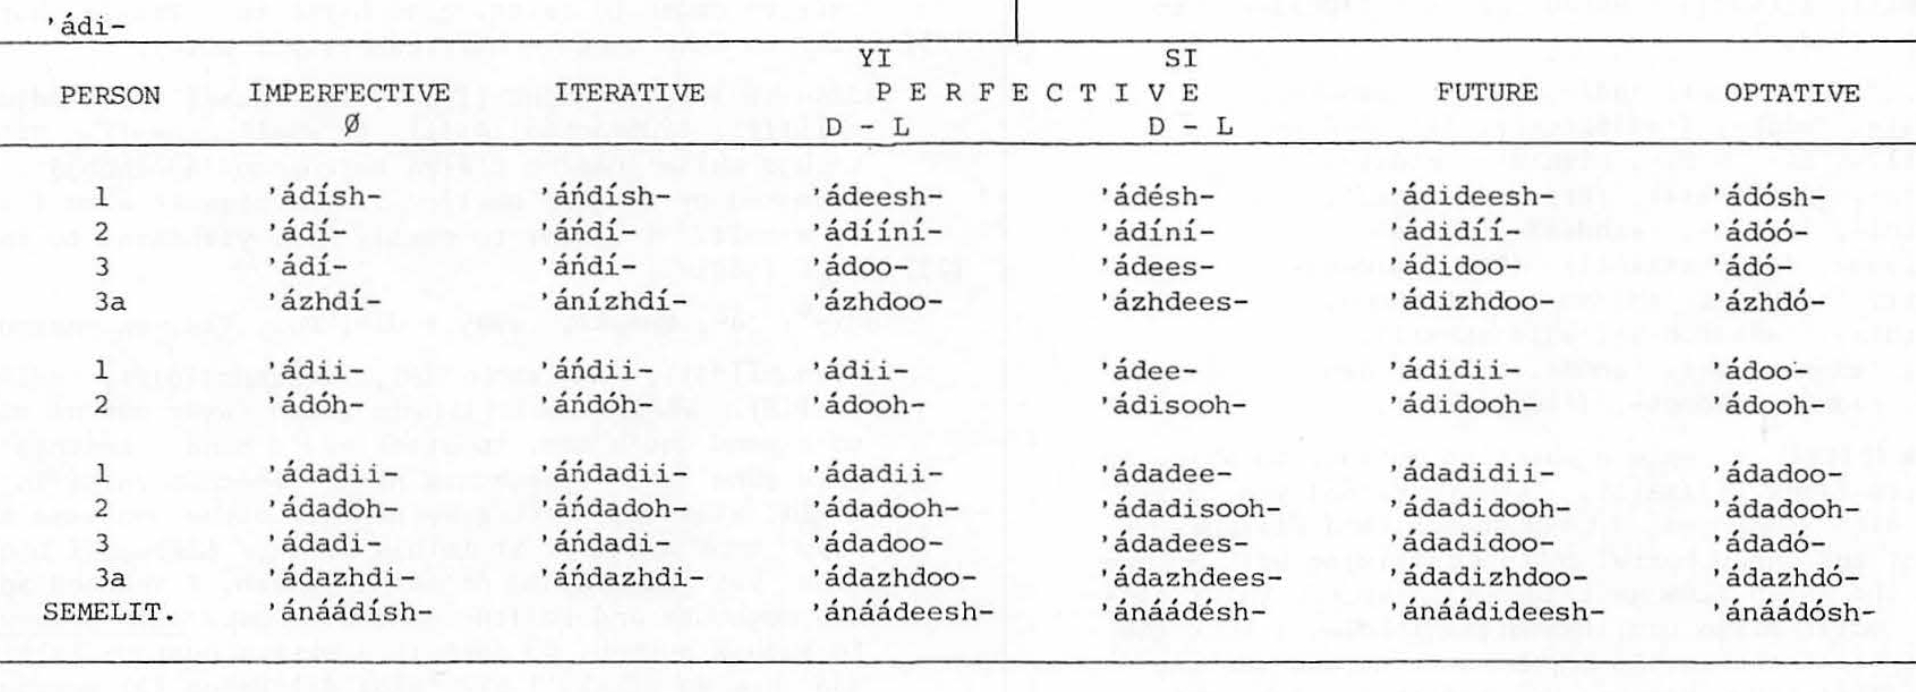
\includegraphics[width=\linewidth]{figures/conjug.jpg}
    \caption{Example of conjugation table for verbs with the prefix string \textit{’ádi-} (\cite[part II:23]{Young:1987uj}).}
    \label{fig:conjug}
\end{figure}

These tables enable users to construct other person/number forms. To form the second-person singular optative of \textit{’ádísk’ąąs}, for instance, one would combine the optative prefix string \textit{’ádóó-} from the table with the stem \textit{k’ąąs}, yielding \textit{’ádóók’ąąs} `you may stretch yourself'. For the Perfective columns, the classifier as well as the conjugation prefixes in Position VII (\textit{si-}, \textit{ni-}, \textit{yi-} or \textit{Ø-}) are necessary to locate the correct form. The perfective form of \textit{’ádisk’ąąs} is \textit{’ádésk’ąąs}, and therefore belongs to the second column of the perfective conjugation, \textit{’ádésh-}, \textit{’ádíní-}, \textit{’adees-} etc. (\textsc{si}-perfective). Phonological processes, such as consonant harmony (changing \textit{’ádésh-} to \textit{’ádés-} before a stem with /s/), must also be applied.

Some entries, like \textit{’ádádiisdzííd} (`I am sipping it'), list their full conjugation paradigm directly if it is not shared by other verbs. The conjugation can be located in an indented part, as shown of the entry of \textit{’ádádiisdzííd} in \figref{fig:adadiisdziid}.

\begin{figure}
    \centering
    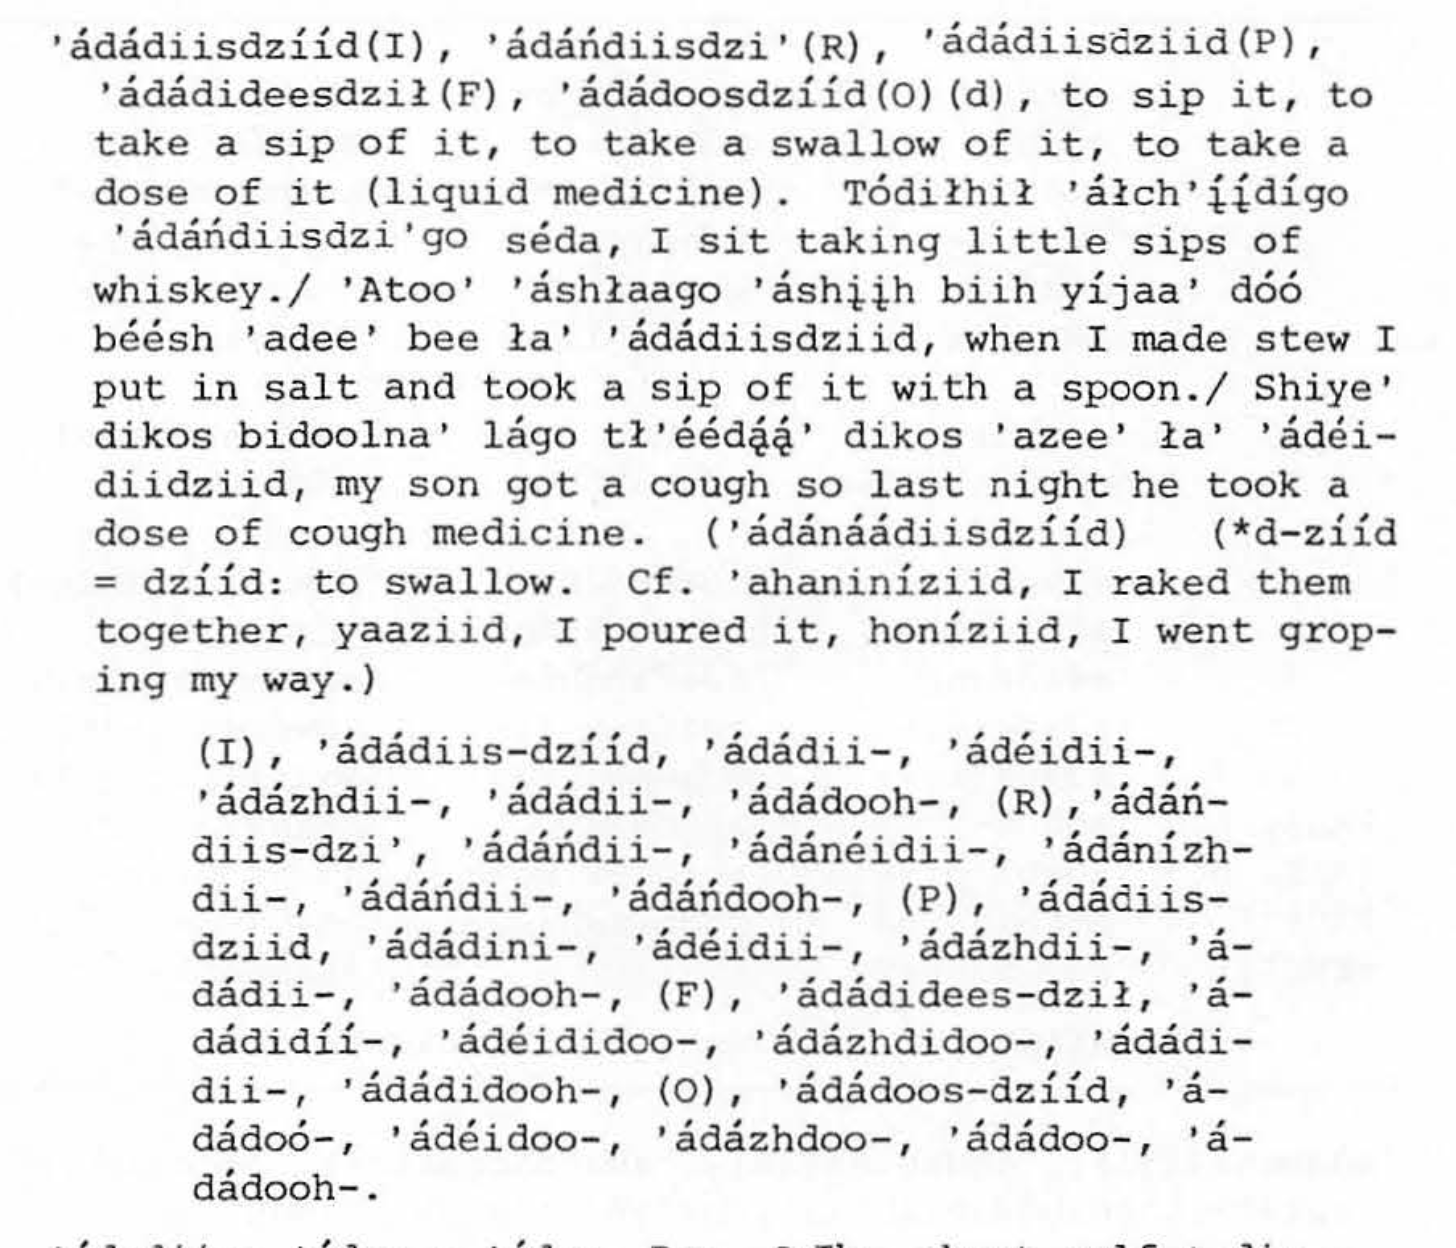
\includegraphics[trim={0 20 0 0},clip,width=\linewidth]{figures/adadiisdziid.png}
    \caption{Example of a verbal entry with its own conjugation in \textit{The Navajo language.} (\cite[7]{Young:1987uj})}
    \label{fig:adadiisdziid}
\end{figure}

The structure of listing verbs in their full form is particularly valuable for working with naturally occurring texts, as it begins with actual word forms. However, for glossing, which requires breaking words into smaller morphological entities, a templatic approach is also necessary.

\subsubsection{Verbal entries in the \textit {Analytical lexicon} (1992)}

The \textit {Analytical lexicon} (\cite{Young:1992bd}) takes a complementary, stem-based approach. Since Navajo verb stems alternate for both inflectional mode and more lexicalized aspectual categories, this organization provides a different analytical perspective. A root entry\footnote{In \citet{Young:1992bd}, the terms ``stem'' and ``root'' are not formally distinguished; both refer to the core lexical morpheme of a verb. However, they employ ``root'' specifically as the dictionary entry that represents the entire set of related inflected and derived stems. This canonical entry is based on the perfective (momentaneous or neuter) stem and is typographically distinguished by capitalization, e.g., ZIID (the root/entry) versus ziid (a specific stem).}, such as ZIID (see \figref{fig:ziid}), shows a complete set of stem alternations across the different modes, but also across multiple aspects (e.g., Momentaneous, Conclusive, Continuative).

\begin{figure}
    \centering
    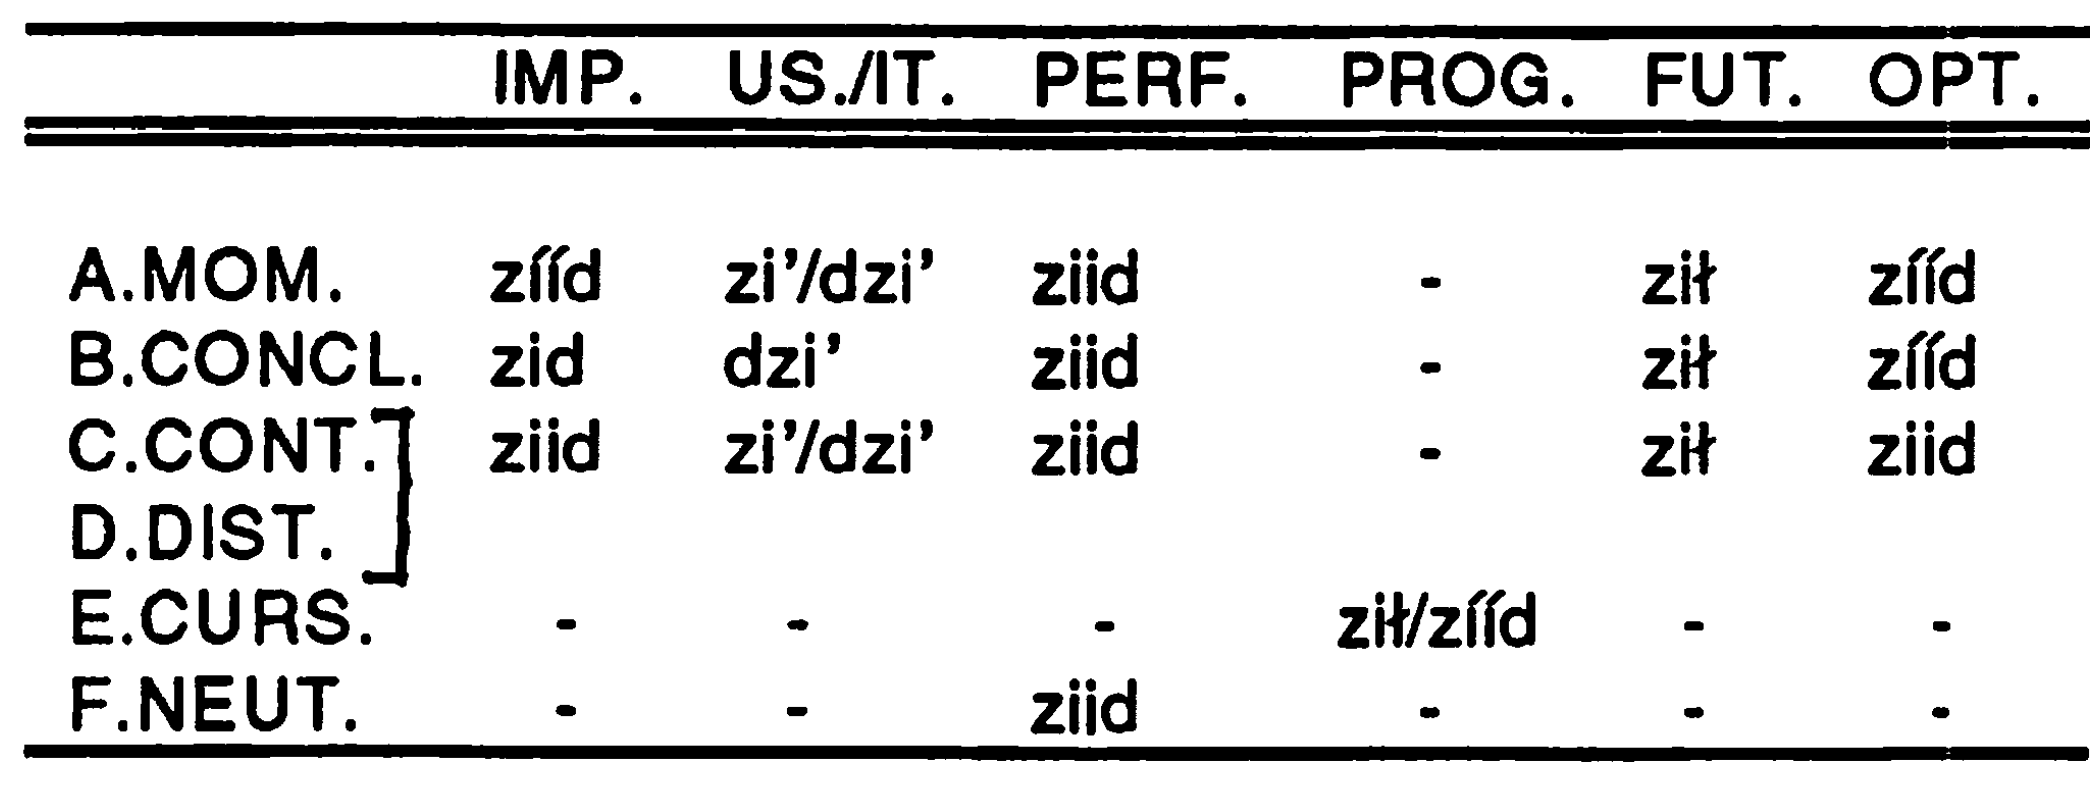
\includegraphics[width=0.7\linewidth]{figures/ziid.png}
    \caption{Stem set of the root ZIID (\cite[749]{Young:1992bd}).}
    \label{fig:ziid}
\end{figure}

Derived verb stems are clustered under one root entry (namely, the stem pertaining to the perfective mode and the momentaneous aspect). Sub-entries specify different aspects, classifiers, and thematic/derivational prefixes, creating distinct verb themes. These themes are cross-referenced to the 1987 dictionary. For example, the verb \textit{’ádádiisdzííd} (\figref{fig:adadiisdziid}) is located under the root ZIID, within the Momentaneous Aspect sub-entry, the D-classifier sub-sub-entry, and the thematic prefix \textit{ádádii-} (see \figref{fig:adadiisdziid-analyt}). Full word forms are reached only after following these analytical steps (Root (ZIID) > Aspect (Momentaneous) > Classifier (D-classifier) > Prefixes (\textit{’ádádii}) > Conjugation prefixes in Position VII (Ø for imperfective and Ø for perfective). However, the entry provides only the imperfective and perfective verb forms. The remaining modes (Iterative, Future, and Optative) are predictable through the conjugation tables in the Appendix or by consulting the corresponding entry in the 1987 dictionary, whose page number (e.g., p. 7) is indicated after the conjugation prefixes (Ø/Ø). This is shown in \figref{fig:adadiisdziid-analyt}.

\begin{figure}
    \centering
    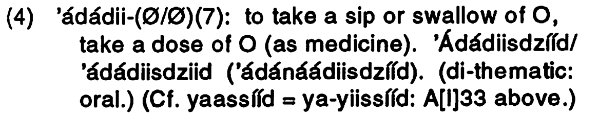
\includegraphics[width=0.7\linewidth]{figures/adadiisdziid-analyt.png}
    \caption{Entry of \textit{ádádiisdzííd} in the \textit{Analytical lexicon} (\cite[750]{Young:1992bd}).}
    \label{fig:adadiisdziid-analyt}
\end{figure}

In contrast, the 1987 volume lists fully inflected forms without analytically separating thematic/derivational prefixes. Consequently, verbs from the same stem but different aspects appear in separate entries. For instance, \textit{bik’éssid} `to pour it over it'; (\figref{fig:bikessid-analyt}) and \textit{’ádádiisdzííd} (\figref{fig:adadiisdziid}) are listed separately in the 1987 dictionary (under ``\textsc{b. conclusive}'' and ``\textsc{a. momentaneous}'' respectively), despite sharing the stem ZIID. In the Analytical Lexicon, they are also listed separately (\figref{fig:bikessid}) but unified under the same stem ZIID which is distinguished by aspect (\textit{’ádádiisdzííd} under Momentaneous, \textit{bik’éssid} under Conclusive).

\begin{figure}
    \centering
    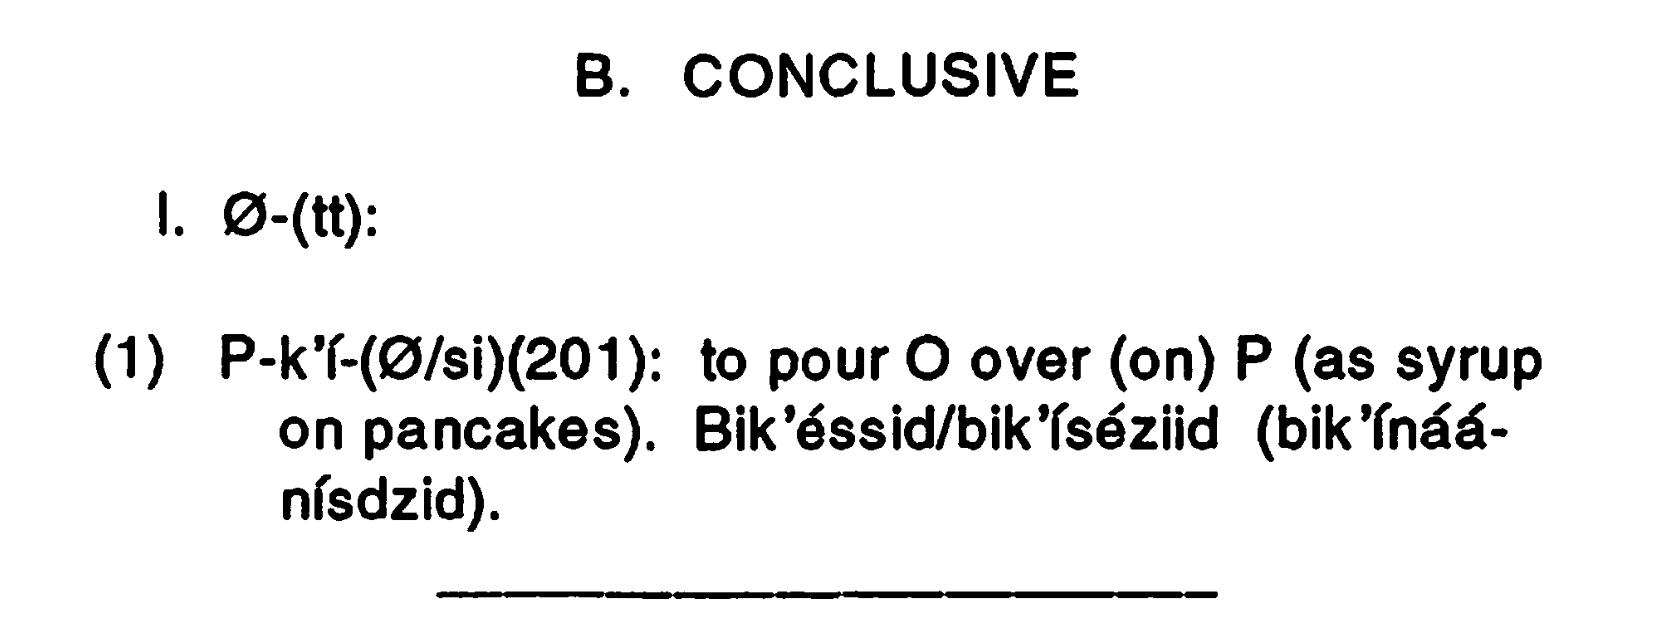
\includegraphics[width=0.7\linewidth]{figures/bikessid-analyt.png}
    \caption{\citet[750]{Young:1992bd} entry of \textit{bik’éssid}.}
    \label{fig:bikessid-analyt}
\end{figure}

\begin{figure}
    \centering
    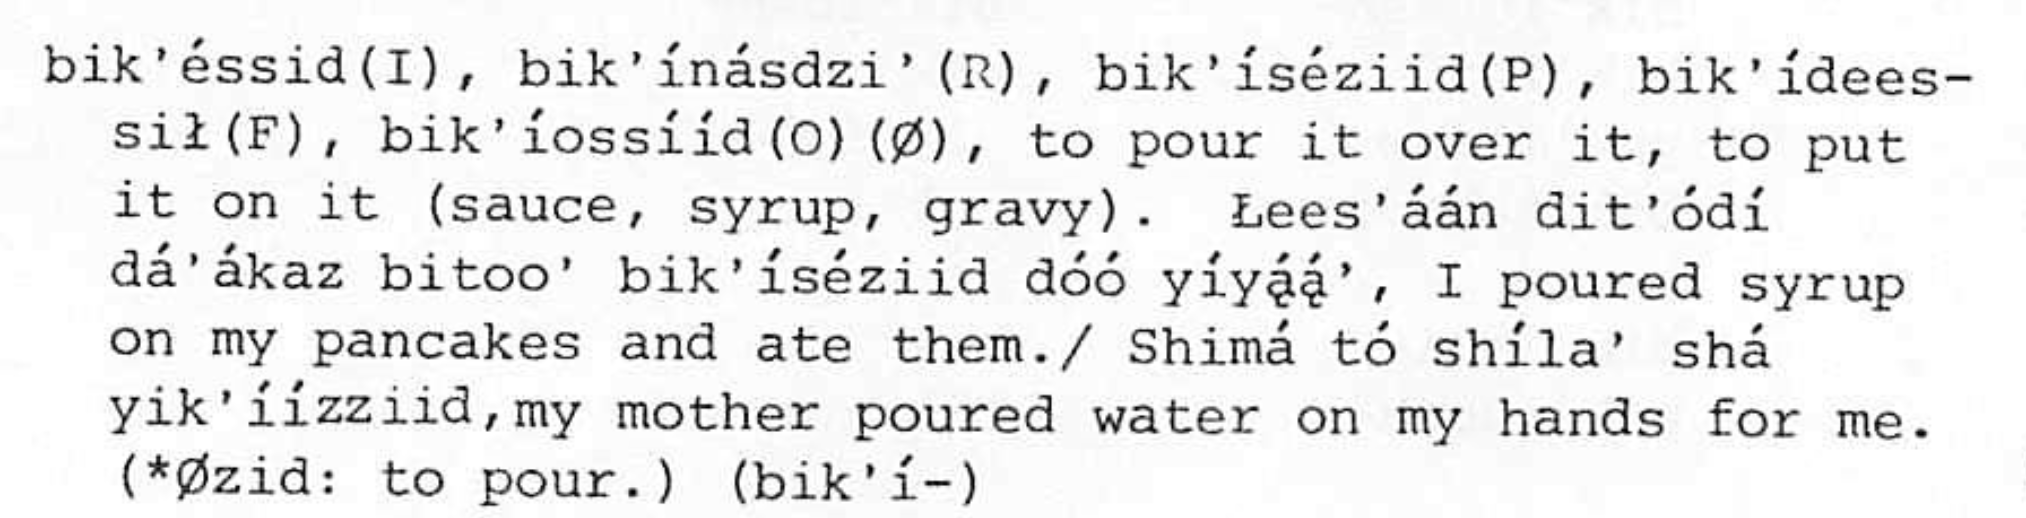
\includegraphics[width=0.7\linewidth]{figures/bikessid.png}
    \caption{\citet[201]{Young:1987uj} entry of \textit{bik’éssid} `to pour it over it'.}
    \label{fig:bikessid}
\end{figure}

The cross-referencing between the two works, where the \textit {Analytical lexicon} provides page numbers to the 1987 dictionary, makes them indispensable companion tools. For this corpus project, both were used extensively. The 1987 volume provided attested word forms and conjugation patterns, while the \textit{Analytical lexicon} supplied crucial information on stems and lexical aspect, which was included in the gloss.

\subsubsection{The bipartite approach (McDonough 1995)}

We have seen that by abandoning the templatic approach to verbs, prefixes are still distinguished from stems, either in a prefix string that is already conjugated (\cite{Young:1987uj}) or a thematic prefix string (\cite{Young:1992bd}). An additional non-templatic analysis is the Bipartite Constituent Model (\cite{McDonough:1995hp}), which is informed by phonological boundaries of surface forms. It proposes that the Navajo verb is built from two core morphological constituents, and a third, outer domain for disjunct clitics. The schema below is adapted from \citet[28]{McDonough:1995hp}:

\begin{center}
    [Disjunct Domain \#  (Agreement) [Inflectional Constit.] [Verb Constit.] ]\textsubscript{Word}
\end{center}

Where:

\begin{itemize}
    \item \textbf{Disjunct Domain:} Clitic-like elements (adverbials, postpositions) attach to the left edge of the core compound. This corresponds to Positions 0-III in the templatic model.
    \item \textbf{Inflectional Constituent:} Contains a portmanteau \textsc{infl} stem (tense/mode{\slash}subject) and qualifier prefixes, with object agreement prefixes added if verbs are transitive. (Positions IV-VIII of the template)
    \item \textbf{Verb Constituent:} Contains the verb stem and classifier prefixes. (Positions IX and X of the template)
\end{itemize}

This model challenges the slot-and-filler template by arguing that phonological evidence points to strong structural boundaries between the two core constituents. Furthermore, grammatical information like tense, mode and subject agreement is fused into single, portmanteau constituents such as the inflectional and verb stem. \citet{McDonough:1995hp} argues for the bipartite model primarily on learnability grounds. She claims the verb structure must be transparent to learners and that morphological information should be recoverable from phonetics and phonology. This morphological and phonological transparency is best communicated when assuming this fundamental distinction between the \textsc{infl} and verb constituent, which aligns with the minimal disyllabic requirement for verbs (see \cite{Speas:1984mo}). The position-class template, in contrast, is an abstract descriptive tool not reflected in lexical patterns or phonological evidence, making it an implausible model for acquisition.

Adopting this learnability perspective, our glossing strategy for the corpus is deliberately surface-oriented. This approach, designed to enhance accessibility for Navajo speakers, is informed both by McDonough's surface-based model and by our adherence to the conventions of the Young and Morgan dictionaries. The rationale for this combined approach is detailed in \sectref{sec:conventions}.

\subsection{Syntax}

The syntax of Navajo does not exhibit many rigid rules or unpredictable behaviors. Navajo is a verb-final language, with agents generally preceding patients; however, the overt expression of both roles in transitive sentences is quite rare. Grammatical relations involving at least one speech act participant (1st or 2nd person) follow a nominative-accusative alignment marked on the verb. In scenarios with only non-speech act participants, object agreement depends on the animacy and topicality of the referents. According to \citet{Willie:2000up}, for third-person referents, entities of higher animacy precede those of lower animacy. Whether higher-ranked entities act on lower-ranked entities or vice versa, i.e., the grammatical roles of agent and patient, is determined by special third-person object agreement on verbs (\textit{yi}- vs. \textit{bi}-, respectively). This is shown in example (\ref{ex:intro2}). Here, `boy' ranks higher than `horse'.

\ea\label{ex:intro2}
    %\textup{Common nouns in A and P roles (\cite[364]{Willie:2000up})}\\
    \ea
    \textit{’Ashkii łį́į́’ yiztał}\\
    \glll \textup{’ashkii} \textup{łį́į́’} \textup{\textbf{yi}-z-tał}\\
	boy horse \textbf{\textsc{3.yi}}-\textsc{3.si.perf}-kick.\textsc{perf}\\
    A P V\\
    \glt `The boy kicked the horse.' %\exsource{overheard conversation}
    \ex
    \textit{’Ashkii łį́į́’ biztał}\\
    \glll \textup{’ashkii} \textup{łį́į́’} \textup{\textbf{bi}-z-tał}\\
    boy horse \textbf{\textsc{3.bi}}-\textsc{3.si.perf}-kick.\textsc{perf}\\
    A P V\\
    \glt `The boy was kicked by the horse.'\exsource{Adapted from \cite[364]{Willie:2000up}}
    \z
\z
    
If the agent and patient rank equally in animacy, the order can be flexible, but topicalized entities always precede those that are focused. For this reason, Navajo is considered a ``Topic-Focus-Verb'' language rather than a ``Subject-Object-Verb'' language.

In addition, Navajo is a pro-drop language. The influential Pronominal Argument Hypothesis (\cite{SandovalJelinek:1989ke}) applied to Navajo (\cite{Speas:1990kf}, \cite{Hale:2006wh}) argues that the verbal agreement prefixes constitute a non-configurational clause, with free nominals as adjuncts. Consequently, the traditional concept of a ``verb phrase'' is not fully applicable to Navajo, as verbs alone can constitute entire clauses. However, \citet{Willie:1995zc} argue for configurationality on the discourse level since the order Topic-Focus-V is consistent. \citet{Hale:2001aq} accounts for configurationality within the verb and posits morphological vP nodes. Beyond the clause, \citet{Hale:1977li} propose phrase structure trees for multiple utterances, showing that while the clausal syntax is flat, there is great complexity within noun phrases, and within verbs. They identify the following phrases: Clause, Noun Phrase, Postpositional Phrase, Enclitic Phrase. 

A noun phrase consists of a noun or pronoun, with additional modifiers that may precede or follow the head noun. Property concepts that modify nouns follow the noun, and since many derive from verbal expressions, the category of ``adjective'' is also not clearly applicable. In noun phrases, possessor nouns precede possessed nouns, and the possessed noun carries a prefix that agrees in person and number with the possessor. A complex noun phrase exhibiting a deverbal noun with multiple modifiers is given in (\ref{ex:intro3}).

\ea\label{ex:intro3}
    %\textup{Complex noun phrase (modified from Tony Tsosie 12.2)}\\
    \textit{Díí chidí naat’a’í ’ayóí ’ádaniłtsxooígíí bitsiits’iin}\\
    \glll \textup{díí} \textup{chidí} \textup{naa-t’a’=í} \textup{’ayóí} \textup{’á-da-ni-ł-tsxoo=ígíí} \textup{bi-tsiits’iin}\\
	this car \textsc{cont}-fly.\textsc{impf}.\textsc{cont}=\textsc{nmlz} very	\textsc{th}-\textsc{distr}-\textsc{th}-\textsc{ł}-be.very.big.\textsc{neu}.\textsc{impf}=\textsc{pres}.\textsc{ref} 3.\textsc{poss}-head\\
    demonstrative noun {deverbal\_noun (possessor)} adverb {deverbal\_adjective} {possessed\_noun}\\
    \glt `These big planes' motors.' \exsource{modified from Text I: \ref{ex:text9-12-2}}
\z

This structure is mirrored in postpositional phrases, where the modified noun follows the postposition, which similarly displays a prefix that agrees in person and number with that noun. Postpositions, however, can also act as adverbs or even be incorporated into the verb, inheriting the agreement prefix.

\ea\label{ex:intro4}
    %\textup{Postpositions (NCHN; TRR1: 36.1)}\\
    \textit{beeldléí yee ’ákászaazgo}\\
    \glll \textup{beeldléí} \textup{y-ee} \textup{’á-ká-s-zaaz=go}\\
    blanket 3.\textsc{yi}.\textsc{poss}-with \textsc{refl}.\textsc{poss}-on-3.\textsc{si}.\textsc{perf}-belt.\textsc{neu}.\textsc{perf}=\textsc{sub}\\
    %blanket {with it} {belted around himself}\\
    noun postposition postposition-verb\\
    \glt `blanket wrapped around his middle.' (lit. `with the blanket it is belted around himself.') \exsource{Text A: \ref{ex:text1-36-1}}
\z

Because the prefixes on possessed nouns and postpositions are identical to object prefixes in verbs, nouns, postpositions and verbs are morphologically connected, which blurs the distinction between different parts of speech. Additionally, enclitics may attach to any of these word classes or phrases. In terms of negation, Navajo employs a preverbal negative marker, often coupled with a second marker at the end of the sentence, creating a bipartite negation structure:

\ea\label{ex:intro5}
    %\textup{Negation (NCHN; CT:2.2)}\\
    \textit{’Éí bízhi’ígíí dóó shash jiníi da}\\
    \gll \textup{’Éí} \textup{bí-zhi’=ígíí} \textup{doo} \textup{shash} \textup{ji-níi} \textup{da}\\
	That	3.\textsc{bi}.\textsc{poss}-name=\textsc{pres.ref} not bear \textsc{anim}-say.\textsc{neu}.\textsc{impf}	not\\
    \glt `One does not mention their name ``bear''.' \exsource{Text F: \ref{ex:text6-2-2}}
\z

\section{Glossing approach in the Navajo Corpus of Historical Narratives}\label{sec:conventions}

Throughout the scholarly tradition of Navajo and Athabaskan languages, linguists have typically avoided exhaustive segmentation, focusing only on categories pertinent to the specific discussion (\cite{Denk:2024aq}; \cite{Hargus:2020wv}). This prioritizes practicality, often simplifying glosses to the word level or omitting morphological detail due to space constraints and audience needs. For instance, the Navajo Conversational Corpus (\cite{Mithun:2009nl}) provides only free translations, and even \citet{Young:1987uj} refrain from full morphemic glossing in narrative examples. As mentioned previously, the central analytical challenge is the morphological structure itself, where lexical, derivational, and inflectional information is spread across verb positions, making a consistent morpheme-based approach inherently difficult.

To address this, \citet{Denk:2025zp} developed a glossing strategy for the Navajo Corpus of Historical Narratives (NCHN) that balances linear analysis with faithfulness to surface structure. The corpus implements this through several annotation tiers:

\begin{itemize}
    \item \textbf{Word:} Presents Navajo words as they appear in the narrative, with minimal corrections for typographical errors.
    \item \textbf{Morpheme:} Displays morphemes in their surface forms (morphs), segmented with hyphens for affixes and equal signs for clitics.
    \item \textbf{Lexical Entry:} Represents the underlying forms of morphemes, with one form chosen as the headword, often based on its first occurrence in the corpus.
    \item \textbf{Lexical Gloss:} Provides grammatical information and English translations following the Leipzig Glossing Rules.
    \item \textbf{Lexical Grammatical Information:} Specifies word-class information for stems and affixes (e.g., verbal stem (v), preverbs (PRVB), postpositions (post)).
    \item \textbf{Word Gloss:} Gives an English gloss for the entire word, capturing its compositional meaning.
    \item \textbf{Free Translation:} Provides a sentence-level English translation, typically retaining the original from the source narratives, unless it has been revised for the sake of clarity; in such cases, this is indicated in square brackets.
\end{itemize}

An example of glossing is given below (the Free Translation tier is omitted as this is a single word):

\begin{table}
    \begin{tabular}{llllll}
        \multicolumn{6}{l}{from NCHN (A Childhood Tale; John C. Claw; 13.26)}\\
        Word: & \multicolumn{5}{l}{ndahaazbą́ą́z}\\
        Morphemes: & n- & da- & haa- & z- & bą́ą́z\\
        Lex. Entries: & ni-\textsubscript{5} & da-\textsubscript{3} & h-\textsubscript{1} & si-\textsubscript{1} & bą́ą́z\\  
        Lex. Gloss: & \textsc{th} & \textsc{distr} & \textsc{ser} & 3.\textsc{si}.\textsc{perf} & roll.\textsc{perf}\\
        Lex. Gr. Info: & v:PRVB & Att. to any cat. & v:QUAL & v:AMS & v\\
        Word Gloss: & \multicolumn{5}{l}{they rolled it one after another up to a point}\\
    \end{tabular}   
\end{table}

As shown, the word \textit{ndahaazbą́ą́z} is linearly segmented and glossed, and abandons distributional or holistic word glosses. Consequently, Young and Morgan's templatic positions became a valuable tool for linearly assigning morphemes. However, we also oriented the linear analysis to the surface structure, similar to McDonough's (\citeyear{McDonough:1995hp}) bipartite approach, and abandoned numerical positions. Instead, we clustered morphs from the \textit{Lexical Gloss} tier into functionally defined categories of the \textit{Lexical Grammatical Information} tier. These categories align with the template but involve different clustering, as shown in \figref{fig:verbtemplate}.

\begin{figure}
    \centering
    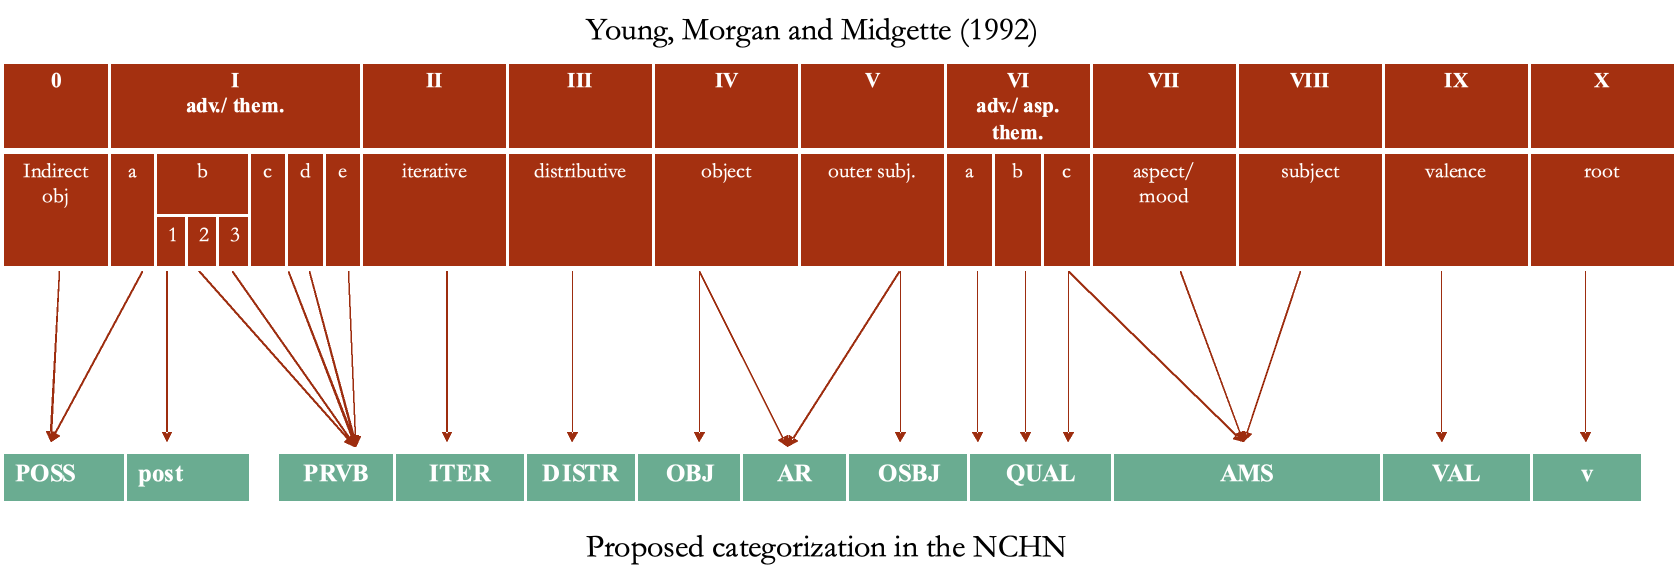
\includegraphics[width=\linewidth]{figures/template.png}
    \caption{Categorization of morpheme positions from \citet{Young:1992bd} in the NCHN (Figure from \cite{Denk:2024aq}). Abbreviations are further explained in the Appendix.}\label{fig:verbtemplate}
\end{figure}

The glossing strategy is governed by three underlying principles:

\begin{enumerate}
    \item \textbf{Surface Faithfulness:} \textit{Do not change the shape of morphs while segmenting.}
    
    Morphemes are segmented in their surface form. For example, \textit{ndahaazbą́ą́z} is segmented as \textit{n-da-haa-z-bą́ą́z}. Variant forms like the seriative \textit{haa-} are registered as allomorphs of a single lexical entry (e.g., h-), with the first corpus instance typically chosen as the headword. In an approach that adopted the Young and Morgan template strictly, this word would be segmented as ni\textsuperscript{I}-da\textsuperscript{III}-hi\textsuperscript{VI}-siV\textsuperscript{II}-Ø\textsuperscript{VIII}-Ø\textsuperscript{IX}-bą́ą́z\textsuperscript{X} (with numbers of positions in superscript).
    \item \textbf{Category Faithfulness:} \textit{Keep number of categories and morphs in a manageable range, and do not merge or split them.}

    This principle streamlines annotation by consolidating morpheme categories to a manageable set, reducing redundancy while ensuring consistent assignment. It overrides exhaustive segmentation where fusion is systematic. For instance, the diverse thematic and adverbial morphemes from positions Ib(2,3)-e in Young and Morgan's template are grouped as a single Preverb (PRVB) category. This grouping of similar categories also applies to postpositions, where freestanding and verb-incorporated forms are glossed identically, as in the following example:\footnote{One difference between the glossed text presented in this volume and the corpus is that incorporated postpositions are still hyphen-segmented here, whereas in the corpus they are treated as stems. Without the hyphen, two morphemes such as \textit {ká} and \textit{s-} would be conflated as \textit{kás-} in the current text, whereas with the hyphen they appear as \textit{ká-s-}. In FLEx, by contrast, the separation is maintained through spaces and multiple tiers of annotation -- a level of detail this volume does not display. Instead of splitting up one word into two words, this approach preserves the integrity of the word as it appears in the original text.}

\begin{table}
    \begin{tabular}{lp{1,1cm}lllp{1,1cm}ll}
        \multicolumn{8}{l}{from NCHN (The Trouble at Round Rock; Mexican Clansman; 36.1)}\\
        beeldléí&\multicolumn{2}{l}{\textbf{yee}}&\multicolumn{5}{l}{\textbf{’áká}szaazgo}\\
        beeldléí&\textbf{y-}&\textbf{ee}&\textbf{’á-}&\textbf{ká}&s-&zaaz&=go\\
        beeldléí&y-\textsubscript{1}&ee&’á-\textsubscript{3}&káá’\textsubscript{1}&si-\textsubscript{1}&zaaz\textsubscript{1}&=go\\
        blanket&3.\textsc{yi}.\textsc{poss}&with&\textsc{refl}.\textsc{poss}&on&3.\textsc{si}.\textsc{perf}&belt.\textsc{neu}.\textsc{perf}&=\textsc{sub}\\
        n&any cat.&\textbf{post}&any cat.&\textbf{post}&v:AMS&v&prt\\
        blanket&with it&&\multicolumn{5}{l}{belted around himself}\\
        \multicolumn{8}{l}{blanket wrapped around his middle}\\
    \end{tabular}   
\end{table}

    Similarly, aspect, mood, and subject markers (from Young and Morgan's positions VIc, VII, and VIII) are fused into a single Aspect-Mood-Subject (AMS) category (aspect, mood, and subject) because they often merge into unsegmentable portmanteau morphs (e.g., \textit{s-} for 3.\textsc{si}.\textsc{perf}). This grouping, acknowledging the fusional nature of this domain as suggested by McDonough's (\citeyear{McDonough:1995hp}) bipartite model, facilitates annotation and retrieval. An example of two consolidated positions is the category of the Areal (AR). These two subject and object uses of the prefix \textit{ha-}/\textit{ho-}/\textit{h-} do not co-occur, and therefore, this prefix has been assigned a single category. Similarly, paradigms that share structural features, like the usitative/imperfective or future/progressive within the AMS category, are glossed as one (imperfective and progressive, respectively).

    \item \textbf{Form-Meaning Exhaustion:} \textit{Segment as much as possible and assign as much meaning as possible to segmented parts.}

    Words are segmented down to single morphs, but not below the surface level. This can lead to what would be a single category in a distributed/holistic approach being annotated in multiple tiers. A clear example is the future paradigm: forms like \textit{díí}- (2\textsc{sg}.\textsc{fut}) are segmented as \textit{d-íí} and glossed as \textsc{fut}-2.\textsc{sg}.\textsc{prog}. This reflects its structural composition from a future marker plus the progressive paradigm as seen in Table 5.

    \begin{table}
        \caption{Future paradigm compared to progressive paradigm (\cite[907,910]{Young:1992bd}). The letter C denotes any thematic consonant preceding the morpheme sequence.}
        \label{tab:placeholder}
        \begin{tabularx}{.6\linewidth}{XXX}
            \lsptoprule
            &\textsc{future}&\textsc{progressive}\\
            \midrule
            1\textsc{sg}&\textit{deesh}-&\textit{Ceesh}-\\
            2\textsc{sg}&\textit{díí}-&\textit{Cíí}-\\
            3&\textit{doo}-&\textit{Coo}-\\
            1\textsc{du}/\textsc{pl}&\textit{dii(d)}-&\textit{Cii(d)}-\\
            2\textsc{du}/\textsc{pl}&\textit{doo(h)}&\textit{Coo(h)}-\\
            \lspbottomrule
        \end{tabularx}
    \end{table}

    This grouping, again, avoids the need for a separate, fully inflected future paradigm (aligning with Category Faithfulness). In addition, a similar principle is used for verb stems, which are glossed for specific sub-aspects (e.g., \textsc{neu}.\textsc{impf}) based on the stem tables in \citet{Young:1992bd}.

\end{enumerate}

In summary, we annotated words according to a linear analysis that oriented itself on the template but included as much grammatical information as possible, resulting in multiple annotation of categories in verbs, without over-exhausting the number of categories. Thus, different from Young and Morgan's analyses of verbs (fully conjugated vs. verb themes), we retained linearity in segmenting the verbs but glossed some the segmented morphs according to categories that might be otherwise considered distributed (such as Continuative, which we glossed for the prefix and the stem). These principles resulted in a practical, user-friendly annotation system that aligns with the template of Young and Morgan while simplifying the relationship between morpheme form and category.

This entire consideration of morpheme glossing and the multiple tiers that we applied to the corpus are essential to understanding the segmentation and glossing in this publication for Open Text Collections, even when more technical tiers like \textit{Lexical Entry} and \textit{Lexical Grammatical Information} are omitted. We acknowledge that the glossing of Navajo and other Dene languages is a controversial issue, not only culturally but technically (\cite{Hargus:2020wv}; \cite{Denk:2024aq}). Nevertheless, we opted for the continuation of the linear approach that we have developed in the corpus because we think that the glossing tier \textit{Lexical Gloss} best captures the categories that a reader is interested in, whether they believe Navajo's categories are templatic or distributed. Readers are encouraged to read the Corpus Guidelines on the webpage of the corpus (\url{https://digitalrepository.unm.edu/navajocorpus/1/}) to get a better understanding of the different glossing conventions.

\section{Provenance}

This publication presents texts from the March 2025 version of the morphologically annotated Navajo Corpus of Historical Narratives (\cite{Denk:2025zp}). The corpus contains Navajo texts that were originally selected, transcribed, and published by Robert W. Young and William Morgan, two foundational figures in Navajo linguistic documentation. The texts come from two collections: \textit{The trouble at Round Rock} (\citeyear{Young:1952cy}) and \textit{Navajo historical selections} (\citeyear{Young:1954jz}), each published by the U.S. Bureau of Indian Affairs. Their works focused on documenting and preserving narratives relevant to Navajo history, culture, and language, as well as introducing accessible Navajo language texts to broader audiences. The Navajo Corpus of Historical Narratives expands on their legacy by providing annotated translations that allow for more detailed linguistic analysis. 
Any additions, changes, or omissions in the free translation are indicated by square brackets in the corpus, and these markings are retained in the ``English translation'' section for each text in this volume.

\subsection{Ethics}

This publication ensures respect for the rights of all contributors and the communities whose narratives and linguistic data are represented. The historical narratives analyzed in this work ultimately originate from Navajo authors from the late 19\textsuperscript{th} and early 20\textsuperscript{th} centuries and have therefore a primary connection to the Navajo community. Through the scholarship of \textit{’Ádahooniłígíí} and Young and Morgan, these texts have been made available to broader audiences. The ethical considerations of that time are not clear.

To ensure compliance with copyright and permissions, due diligence has been conducted regarding the legal status of these materials. Correspondence with relevant administrative bodies, including the Indian Bureau of Education, has indicated that these works are in the public domain, and additional confirmation has been sought from the U.S. Copyright Office to ensure the publication's adherence to copyright regulations. Given these findings, the decision has been made to publish this work as an open-access resource, to ensure accessibility and scholarly integrity.

\subsection{Young and Morgan's historical selections}

The selected narratives from \citet{Young:1952cy,Young:1954jz} offer perspectives on historical events and daily life at the end of the 19th century. Texts from \textit{The trouble at Round Rock} (\citeyear{Young:1952cy}) focus on a specific historical incident, namely a dispute involving Agent Shipley and Black Horse, set against the social and economic backdrop of the Navajo Nation. The narratives from \textit{Navajo historical selections} (\citeyear{Young:1954jz}) cover a broader range of topics, including traditional stories and individual experiences that contribute to a more nuanced understanding of Navajo life and worldview. The narratives chosen for this corpus reflect our intention to represent a broad number of topics that could serve as a basis for studying different narrative styles.

\subsection{Selection criteria}

The selection process focused on ensuring diverse representation across different themes and perspectives within the Navajo community. From \textit{The trouble at Round Rock}, all relevant texts were included to provide a complete view of the central historical incident described. For \textit{Navajo historical selections}, texts were chosen to represent each part of the thematic volume, focusing on narratives that include traditional stories, social commentary, personal anecdotes, and historical insights. This includes different narrative styles, such as first- and third-person perspectives.

\subsection{Selected texts}

A total of 9 texts were selected from the two volumes. Texts \ref{chapter:text01}-\ref{chapter:text03} are from \textit{The trouble at Round Rock}, and Texts \ref{chapter:text04}-\ref{chapter:text09} from \textit{Navajo historical selections}.

\begin{table}
    \caption{The texts in this collection.} \label{tab:texts}
\begin{tabularx}{\textwidth}{llQr}

    \lsptoprule
        \textsc{text} & \textsc{title} & \textsc{author}&\textsc{words}\\
    \midrule

		\ref{chapter:text01}&\textit{The trouble at Round Rock} & Left-Handed Mexican Clansman &2,820\\
        \ref{chapter:text02}&\textit{The trouble at Round Rock} & Howard Gorman &787\\
        \ref{chapter:text03}&\textit{The trouble at Round Rock} & The Nephew of Former Big Man&722\\
        %\midrule
        \ref{chapter:text04}&\textit{The traditional Navajo country} (part I)&no author specified&1,049\\
        \ref{chapter:text05}&\textit{The first mother-in-law} (part I)&Tony Tsosie&640\\
        \ref{chapter:text06}&\textit{A childhood tale} (part II)&John C. Claw&2,036\\
        \ref{chapter:text07}&\textit{Our abuse} (part III)&Dan Phillips&1,268\\
        \ref{chapter:text08}&\textit{The special grazing regulation} (part III)&The Blind Man's Daughter&258\\
        \ref{chapter:text09}&\textit{I flew over Navajo land} (part IV)&Tim Yazzie&1,194\\
    \midrule    
        \textbf{Total}&&&\textbf{10,774}\\
    \lspbottomrule
    \end{tabularx}
\end{table}

\section{Genres, styles and main themes}

The genres within the corpus range from historical accounts and adventure tales to traditional narratives and personal recollections. Narrative styles vary accordingly, with some texts taking on formal, descriptive tones, while others exhibit conversational or introspective qualities. The variation in genres and narrative voices provides a broad spectrum of discursive forms, including dialogue, descriptive passages, and self-reflective commentary. The corpus thus promotes, if limited, a diverse representation of themes from the larger pool of narratives, and is a valuable resource for studying Navajo grammar, stylistics, and narrative construction, as well as for understanding the cultural contexts in which these narratives are embedded. The main themes of the narratives are discussed in \sectref{sec:themes}.

\section{Speakers/narrators}

As listed above, the narrators include both named individuals and anonymous voices. Texts in \textit{The trouble at Round Rock} feature historical figures recounting first-hand experiences, while selections from \textit{Navajo historical selections} highlight a range of storytellers, including John C. Claw and Tony Tsosie, who bring personal history and traditional knowledge to life. In addition, it is worth mentioning that traditional knowledge, even if kept distinct from individual tales, exhibits the diversity of families passing these stories to their offspring and therefore also personal accounts and interpretations. As such, the autorship of traditional stories includes an entire chain of past narrators.

\section{Main themes}\label{sec:themes}

The texts enumerated story above in \tabref{tab:texts}, exhibit the following main themes, portrayed in \tabref{tab:themes}.

\begin{table}[]
    \caption{Distribution of main themes across the narratives}
    \label{tab:themes}
    \begin{tabularx}{.85\textwidth}{Xlllllllll}
        \lsptoprule
        \textsc{main themes}&\ref{chapter:text01}&\ref{chapter:text02}&\ref{chapter:text03}&\ref{chapter:text04}&\ref{chapter:text05}&\ref{chapter:text06}&\ref{chapter:text07}&\ref{chapter:text08}&\ref{chapter:text09}\\
        \midrule
        \textsc{historical events}&\times&\times&\times&&&&\times&\times&\times\\
        \textsc{politics}&\times&\times&\times&&&&\times&\times&\\
        \textsc{individual experience}&\times&&&&&\times&\times&\times&\times\\
        \textsc{adventure}&&&&&&\times&&&\times\\
        \textsc{traditional knowledge}&&&&\times&\times&\times&&&\\
        \lspbottomrule
    \end{tabularx}
\end{table}

The main themes are well distributed across the corpus, focusing on experiences on the individual and collective level. In the following, these themes will be commented on in relation to the texts.

\subsection{Historical events and politics}

\textit{The trouble at Round Rock} versions (Texts \ref{chapter:text01}, \ref{chapter:text02}, \ref{chapter:text03}) focus on historical events and political tensions affecting the Navajo people during the late 19th century. The core of these stories revolves around the conflict between Agent Shipley and Black Horse, which instantiates broader socio-political struggles and the tensions arising from U.S. government encroachment. These narratives not only recount specific incidents but also show the effects of imposed policies on the Navajo way of life and governance. They highlight clan leaders and influential community members who are forced to act due to external pressures, providing a Navajo account on the political resistance.

The \textit{Navajo historical selections} volume offers additional political commentary, notably in \textit{Our abuse} (\textref{chapter:text07}) and \textit{The special grazing regulation} (\textref{chapter:text08}). These narratives focus less on the unfolding of historical events but instead more on government-imposed regulations and their consequences for Navajo lands and livelihoods at the time of narration. Dan Phillips, for instance, describes the hardships and frustrations of the Navajo community as they faced restrictive grazing regulations, which drastically altered traditional livestock practices. These stories account for the ongoing tension between Navajo self-governance and federal oversight, tying back to earlier conflicts like \textit{The trouble at Round Rock}. Finally, Tim Yazzie's account on his flight over the Navajo Nation to deliver aid (\textref{chapter:text09}) relates to the historical ``Blizzard of 1949'' and intersects with the livestock reduction policies.

\subsection{Individual experiences and adventures}

Individual adventures are recounted in many of these narratives and provide personal perspectives on broader historical themes. For instance, \textit{A childhood tale} by John C. Claw (\textref{chapter:text06}) describes formative events and challenges faced by the narrator during his early years and highlights how historical events intersected with personal development. Similarly, \textit{I flew over Navajo land} by Tim Yazzie (\textref{chapter:text09}) offers a more immediate account of adventure and the dangers of being on a plane mission. Yazzie's narrative stands out for its sense of freedom and exploration, as he describes the landscapes and people he encountered from an airplane, providing an almost ethereal view of his homeland. These personal reflections lend an intimate tone to what is also a historical event, namely the severe Blizzard of 1949. Furthermore, the stories \textit{Our abuse} (\textref{chapter:text05}) and \textit{The special grazing regulation} (\textref{chapter:text08}) provide individual insights into the hardships faced during the Livestock Reduction Policies. Lastly, the first version of \textit{The trouble at Round Rock} (\textref{chapter:text01}) can also be regarded as an individual experience, since Left-Handed Mexican Clansman was present during the fight between Black Horse and Agent Shipley.

\subsection{Traditional knowledge}

In \textit{The traditional Navajo country} (\textref{chapter:text04}), the anonymous narrator explores the Navajo connection to their land and emphasizes the cultural and spiritual significance of the geography around them. This piece promotes traditional knowledge, as the narrator details the mountains, plants, and animals with reverence and precision. By narrating the symbolic meaning and traditional uses of different elements in the environment, this text helps understand Navajo cosmology and the land as a source of identity and wisdom.
	
Similarly, \textit{The first mother-in-law} narrative (\textref{chapter:text05}) emphasizes traditional customs, such as family roles, marriage, and respect for elders and deities. These stories are not only informative but also preserve the cultural practices and beliefs that define Navajo social life. Tony Tsosie's perspective sheds light on the dynamics of family relations and their societal expectations. Also, John C. Claw's childhood story (\textref{chapter:text06}) incorporates elements like taboos which can be counted as part of the traditional narrative inventory.

Having established the main themes of the collection, the focus now turns to the primary sources themselves. Part \ref{part:texts}, allows these works to speak for themselves, giving the reader direct access to their voices and stories in full detail.


\renewcommand{\exfont}{\itshape}%text line of examples appears in italics
\let\eachwordone=\normalfont\rmfamily%morpheme segmentation line (2nd line) appears in roman font.

\part{Texts}
\label{part:texts}
    \renewcommand{\thechapter}{\Alph{chapter}}
    \setcounter{chapter}{0}
    \chapter{\textit{The trouble at Round Rock} – Left-Handed Mexican Clansman}\label{chapter:text01}
    \setcounter{equation}{0}
        \tocless\section{Summary \& background}
            This narrative portrays escalating tension between the Navajo leader Black Horse and the Navajo Agent Dana Shipley. Agent Shipley is sent to Round Rock to execute the law passed in 1887 according to which all children needed to attend school. The fight starts with verbal exchanges and intensifies into physical confrontation, until Black Horse challenges the authority. Amid the chaos, notable figures, including Sucker and Chee Dodge, strive to temper Black Horse's aggression and mediate peace. When soldiers arrive, both sides brace for conflict, yet the appearance of a War Chief (Officer) shifts the course, leading Black Horse to lay down his weapon and extend a handshake to signal the end of hostilities.

This version focuses on the immediacy of the conflict as a fierce struggle for identity and collective resistance and is therefore more politically charged than the other versions of the Trouble at Round Rock. Left-Handed Mexican Clansman, a witness to this historical event, presents Black Horse as a heroic figure who battles against the colonial forces with emotional stakes involved in the struggle over education. Concluding with \textit{Íídą́ą́ t’ah chąąmą’ii nishłį́įgo, éí t’éiyá biniiyé ’áadi ’atah nahashłe’} (`At that time, I was just a young punk -- that’s probably why I was just there with the crowd for fun'), the author suggests that his perspective on the event may have evolved since then.
        \tocless\section{English translation}
             My forbears, the old men and women folk, were of the Mexican People Clan. With great hardship they came back from the place called Fort Sumner, packing their goods on their backs, and afterward lived here at Lukachukai. Here they began life anew. Then from their home at a place called Spring in the Clay they started moving over and across yonder mountain. While they were making this move they stopped for the night, and it is said that I was born where they halted.

Let's see, I believe it was in the month of October I was born on a night when a heavy snow had begun to fall. My grandfather, a man by the name of White Mexican Clansman, and another man called The Son of Former Sweathouse, were the only men. They and several womenfolk worked hard on me.

My grandfather had a fine wether goat that he was quite proud of. He killed it there, and the people feasted with great joy. Then on the day following the night of my birth we again started to move. In those days people went about only on horseback or afoot.

On the day following the night on which she gave birth to me, my mother went on foot as far as the people moved that day. And since it had snowed the night before they had to go through the snow. It is remarkable how risky life was in those days. Nowadays when a woman gives birth they take special care of her, telling her not to catch cold. Back at that time it was different.

As time went on I somehow grew up. I do not remember much about it. I do not remember in detail much of what happened before I was about ten years old. When morning would come and I would be sleeping nicely, my grandfather would throw me out of bed.

``Come on! Come on! Why are you lying down? Go run a race. If you're weak the first harmful thing that comes along will run over you. If you are strong you will lie hudled in death only after the dirt is torn and furrowed around you (i.e. you will give up only after a struggle),'' my grandfather used to tell me. The old folks all used to say that.

They probably said this because they knew of the wars that were going on. That is the way my grandfather drove me about and spoke to me. He did not speak in anger. He did not speak harshly. He told it to me in a nice way. So that is the way I spent my days from that time on.

After I had reached the age of eighteen I did various kinds of odd jobs. I had an uncle by the name of Forked House. He was a young man, and he adopted me. He started sending me on chores. I would take care of his horses for him. He had a wagon and a team. He would tell me to haul wood with it, or to work with it.

At the time I was about eighteen years old the person who started the present trading post at Blue Clay Point moved there -- I used to know just when it was. They used to call the Former Old Interpreter (Chee Dodge) Chee (Red) when I first heard of him. Chee was a good friend of a white man from Ugly House (Manuelito, N.M.) known as Big Lump Setting Up (S.E. Aldrich). Finally the two of them built the trading post at the place called Blue Clay Point. It was in the Spring when they moved there. There was an epidemic in progress, and we now refer to it as ``the time when the throat killed many.'' It was at that time, in the spring, that they moved to Blue Clay Point, it was said. That is how it came about that the one who would be called The Interpreter (Chee Dodge) and the one who would be named Big Lump Setting Up came to move there.

They built the trading post and four years later perhaps, I do not recall exactly when, the one I called my uncle told us to haul wood there. They (the traders) probably called for the wood.
There was a boy of the Big Water Clan with whom I always chummed around. We started doing that kind of work. We went about calling each other ``younger brother,'' and we hauled wood to the trading post. We heard reports that there were people going about to get children put into school. It was said that they were then over at Chinle, and we heard that they were coming here sometime soon. We would discuss it when we took the wagon after wood.

``Say, let's go to school,'' I said to my companion.

``All right,'' he said.

And we went about, talking enthusiastically about it. In the evening after we had unloaded another load of wood we started back home in the wagon. When we got back to the hogan we found that my uncle was there. And it turned out that my grandfather, who was called Big Mexican Clansman, was there too. So we told them of our plan. ``They are putting chidlren in school, it is said.'' We told them how we had both said, ``Let's go to school.''

``It's probably all right. It's fine indeed, my children. A party is in its way coming to us. You cannot escape them anyway,'' my uncle and my grandfather said to us.

On the next day we went to the trading post, and my grandfather put his thumbprint on a paper for us. It was reported that the children from Chinle who were being taken to school would get there in two days, and we heard the grownups talking to one another about it.

Of those menfolk who were talking to one another about it, one was called Weela. He lived over behind Round Rock and was one of the leaders at that time. One was called Bead Clan Gambler, and he was a member of the police force. He was a very strong, husky man. He was from Chinle, but he was a member of the police force at Fort Defiance. He had come on ahead with the white man from Fort Defiance called Little Chief (Agent Dana Shipley). It was there that my grandfather spoke and promised us.

``I am putting these two boys in school.'' he said by way of promise.

Since it was reported that it would be another day before the wagon load of children would arrive, we went back home. We spent the night there and then returned on foot.

And we found that the children had arrived. There was some man of the Bitter Water Clan whom people called Pug Nose. He was going around with the party, taking care of the children. He knew a little English, and that was probably why he was told to take care of the children. He was busily running around the children who had been hauled in, chattering in English. He was keeping them together. The children from Blue Clay Point who were to be put in school had not all been brought in as yet. It was said that the wagon with the children would start off in two days. They were to go by way of Lukachukai, Tsaile, and Crystal, and on over to Fort Defiance. That was probably their plan.

But the people who live over beyond yonder mountain in the area of Cove and Red Rock were thinking ugly thoughts about the plan in connection with education. It is just recently that these people became old men, and they have all died. At that time, when they acted as they did, they were young men. They said that if this business of taking children to school got to them they would really do something about it. As we came to find out, they were saying that (the school) would not get a one of their children. A man by the name of Black Horse was the leader of that faction. They had no doubt heard that in a certain number of days a party would come to Blue Clay Point for the purpose of putting children in school. So they began to think of the matter with bitterness.

``Boys, let's go there. Come on!'', they probably said. So they probably set out from there for this purpose (of opposing the placing of children in school). We had not heard of this and knew nothing about it. They met (the school party) at Blue Clay Point. 

Near the trading post there was a house which at that time, we called the Ugly House. The house served the purpose of providing a place to sleep for the people who came to the trading post. Black Horse's party went over there, and they no doubt came with evil thoughts. The people who lived hereabout had heard nothing of their plans but at night they spoke about themselves, revealing their intentions.

The one I referred to as my grandfather, and another uncle of mine called Little Boy, apparently went there at night and heard them telling about it. Among those present were the men known as Black Horse, Limper, Tall Red House Clansman, Old Bead Chant Singer -- who was of the Red House Clan -- and his cousin, a Bitter Water Clansman called Bead Chant's Nephew, and another man with whom I was merely acquainted, and who was a relative of mine by marriage. His name was Yellow Fermentive Chewer. These are the only ones I can remember of those who came from there (on the other side of the mountain). I do not remember who the rest were. They probably planned to go in to see the Agent on the next day. They no doubt told what they thought -- what their opinions were regarding this school business that had started in connection with us. They told these things to the people from here who had gathered. So people began to think along the lines of their planning. ``Now men, is there anyone here who can do it (a chant)? Long ago, people of old had a story of some kind of chant called `Talk One Into the Grave.' Who of you knows it?'' said Black Horse, asking that it be perfomed. 

These people from the other side of the mountain were saying this. This is what that is what I heard. I wasn't at the meeting myself. And I don't know just how this chant goes.

``I do,'' said the one I referred to as Little Boy.

``Two of you are needed for it,'' said Black Horse.

So then my grandfather, the man I spoke of as Big Mexican Clansman, volunteered to join him to carry on the ceremony. South from the trading post there is a ruin which we call in Navajo ``Shattered House.'' Someone burned it long ago. It is said that they were Anasazi. It is black there like ashes. It was there that they carried on the ceremony. I don't know how it was done. That is what took place that night.
As for us, we spent another night at my uncle's hogan. Today we had been placed among children who were to be taken off to school. On the morrow we would start off with them. So for that purpose, in the morning we again started off from the hogan afoot. We left with menfolk, with the one who would thumbprint the papers for us and who would vouch for us. It was my grandfather, Big Mexican Clansman. He stood up for the two of us.

When we got to the store we found that many people had assembled. Many horses were standing about. At that time horses were the only means people had for transportation. Some of us did not know what had been done the night before. Someone by the name of Black Horse had brought a party from the other side of the mountain. That is all that we found out.

We were told that now there would be work here making out papers for more of our children. There were three Navajo policemen there in that connection. One of them turned out to be Bead Clan Gambler, one was Singed Man from Fort Defiance -- he was also known as Son of Former Rag Man. Another was Interpreter's (i.e. Chee Dodge's) brother-in-law, a Red Streak Into Water Clansman. This man was killed recently at St. Michaels at a rodeo. He was killed by a racehorse on the track during the race. At that time he was a policeman. I can't think what his name was -- I merely knew him by sight. He was merely called Interpreter's Father-in-law: He was a policeman back at that time. So there were three policemen. It happened that way. Then we were told that the time had come. We saw the people going inside the trading post, so we just went with the crowd. We two who were going to school stayed together. As for the rest of the children who were going to school, I don't know anything about them.

At the time we had brought the last load of wood; while we were unloading it we noticed two women leading a horse nearby. They were probably on their way home. One of these women had promised her son for school. [His name was Toohnii and she had promised him for school] The woman glanced our way. Her name was Red Buttock Clan Woman. She is still living and her hair is white. As she passed by she said, ``It is said that those boys who are unloading wood over there have been promised for school -- they will go to school too. Golly, why they are big enough to be of use here now'', she said of us. I don't know what she had in mind in so saying. We just laughed about it afterward. But that was right. We had volunteered for school. We were going to get an education. We considered school as good news. That was what I thought. I always told my friend about what I myself was thinking. ``You see, it's something to strive for and covet. Look at Chee's trading post here. Quite some time ago when they moved back from Fort Sumner he had a hard time. He started his life by poking around in the horse manure in a stable. He used to be out there early in the morning with a stick especially made for that purpose. He could be seen sitting out there silhouetted against the sun, with the light shining red through his hair. This is how he came to be called Chee (Red). Then some white people took him in. That is how he got his start in life. That is how his mind began to develop. He got ahead and now here he is in his enviable position. He knows English'', I said. That is what I had an ambition to do at that time. It was for that reason that I volunteered myself for school. And the person who had joined me thought likewise. With this in mind I wanted an education badly then. But it was destined to turn out differently.

The people went into the trading post. It was packed full. Over here on one side the counter ran. Further back in the room was a swinging gate. It was out through there that Chee came. The brother of The One Who Has Eyeglasses (John Lorenzo Hubell) from Ganado, a man called the Bat, was a clerk there. He was over to one side behind the counter. The Bat was a man who could understand Navajo very well. A little later the one called Little Chief (Shipley) came out and stopped beside Chee. Chee was his interpreter as he began to make a speech to the people. Black Horse was standing against the counter over to one side. The people of his band were standing with him. The people who had promised their children for school were named, and we were told many things about the school.

Then Black Horse spoke up and said, ``This business of taking children away from people to put them in school -- when is it going to affect the people from over beyond the mountain?'', [he said].

``It will reach you sometime. Tomorrow these will start out and will be routed right along the mountainside'', said Little Chief (Shipley)

``We'll not give you a one of our children. And we'd just as soon fight over the matter as not'', said Black Horse balking stubbornly.

Speaking this way to each other the Agent and Black Horse exchanged many words.

The one I referred to as Limper was standing near Black Horse with a blanket wrapped around his middle. And those of this band were lined up, one behind the other.

``Come on, you boys. Remember what you said,'' said Black Horse.

The one called Limper was the first to hop in there, and he grabbed the Agent by the collar. Then they all rushed in. Chee jumped over the gate at the back of the room, and chaos followed.
``Outside with him!'' voices were saying.

They started out with him. As they were taking him outside I crawled and squeezed myself out among them. Just then they locked the door from the inside. Two of the boys who were going to go to school were locked in. The one I referred to as River Man, who is now known as Short Hair, and another boy with him. These were the ones who were locked inside. On account of this fact the man I spoke of as Weela took the Agent's side -- it was because one of the boys locked in there was his son.

The mob was carrying the Agent away. Not far from there, there was a drop. There was a wash in the blue clay with a point of land on either side. That is how the trading post got its name. It was a long drop.
``Throw him down there! [Down there, down there!]'' voices were heard saying.

A lot of people were standing alongside the trading post, and I among them. My uncle was standing beside me, and I don't remember who else was standing there. As the people carried the Agent along they beat him with their fists. They were beating him up. But as they carried him further away the one called Bead Clan Gambler went running from here where we were standing.\footnote{The English translation in \citet[27-29]{Young:1952cy} continues here with approximately two pages of narrative describing additional events surrounding the fight, including the most violent scenes. Because no corresponding Navajo text is provided in the original source, these passages have been omitted from the present edition. The translation resumes at the next point where the Navajo original is available.}

Over to one side of Black Horse the people were merely milling around. All of them had their horses standing there nearby. Many more joined him, and among these were some women. These women too had spent the night there with them. They had stayed to cook for the men. One of these women had come from over beyond the mountain. I don't know exactly where she came from.

When this happened Black Horse's henchmen spoke without effect because there were others who were trying to keep order and who said ``No'' to the proposal to attack the soldiers.

I was one of those who came back (on the next day) to where the people were. And I found that the people from beyond the mountain -- those among whom the news had been spread, and who were sent for -- had arrived. They had guns and bows and arrows. These were many people. There were also many of us who had joined in just as spectators.

A man of the Salty Water Clan whose name was Slender Lava had his family there, and his wife cooked all night for the men who were making the trouble. In the morning the women again prepared food for them. Then the people noticed that the soldiers were moving along over there.

``All right now! All right! We'll take them right over there in the flat. All right now! Before they move in! Before they move in! Let's get them!'' said Black Horse dashing about but without effect.

But his boys were really impatient. They were rubbing their guns. Then the one to whom I referred as Slender Lava said, ``No!'' He spoke thus because he knew they lacked the wherewithal to win the fight. A man of the Water's Edge Clan, called Sucker, also said, ``No!'' And of the men from hereabout with whom I came and who I mentioned before, my uncle joined in saying, ``No.''

``Wait. Wait. Speak no more like that, my Elders, my friends,'' people said, opposing them.

Then the person whom I said was known as Sucker was sent to the trading post. The soldiers moved into the trading post. They had pack mules, And there was a line of these animals far into the distance. I don't remember what the number of the soldiers who arrived was said to be. I can't recollect. But when they had moved into the past, Sucker was sent over there. Presently he came back from there on horseback.

``They say to wait, boys. They say to wait,'' she said.

Then Black Horse's boys really became impatient. They sent Sucker back over there again.

``Go over there now and tell them, `No'. Tell them not to give us that kind of talk.

Tell them it's going to be now. We'll tear the building to pieces. What can they do? Go tell them that's our answer,'' said Black Horse.

Sucker galloped over there and told them that, and then he returned at a gallop.

``They tell you to wait. The one who says that is the leader of those solders who arrived and he is a War Chief (Officer). It is not the man you threw out yesterday who is saying that,'' he said as he ran back again on horseback.

Then the men over on this side said, ``It's a fact. You never know. You don't know what they have in mind in saying this -- they might have a better idea for settling it. So don't say anything,'' said those on this side who were acting as go-betweens.

Finally many of us started over there, some on foot and some on horseback. We got to the trading post. The soldiers were there on the inside. There were many pack mules, more than twenty I guess. They had all been inside the wool storage shack, with their packs still on. Across from the wool storage shack a gun had been placed to cover its approaches. So in case Black Horse carried out his threat, the soldiers were ready.

Sucker rode over there to where Black Horse and his band were.

[`Now you can come over',] the War Chief (Army Officer) says, [...] `but come slowly, slowly','' said Sucker. 

That's what he reported to them. Then across and opposite us on the other side of the pace called Blue Clay Point horses were seen to be going, and many people too. There were more than twenty. They could be seen going up there over the crest of the hill. People watched and wondered if they had just decided to go back home. But they moved on over the hill and then turned and started coming in this direction along its base. Over here on this side the soldiers were all prepared and were inside the trading post. The entrance way was large, and on both sides of it soldiers were stationed. Over there on this side the people were impatient to shoot. They were really stroking their weapons. They were rubbing their guns, it is said. They were really foolhardy -- at least that's what the spectators were saying.

The white man called The Bat used to say that he was on the soldier's side ``I too had my gun ready like this,'' he used to say.

People would laugh at him when he told about this. He was a trader.

``If they appear over the hill -- if they're serious in their threat -- if they come close, I'll go out there in the open to meet them,'' said the War Chief (Officer). ``If they are serious about it, and if one of them aims at me with one of those guns you see them holding up out there, all of you fire a volley at him,'' said the officer. That was the plan on the inside.

Then they appeared, coming over the hilltop. They were coming toward us. At this point Sucker rode back and forth telling them to take it easy. That was the one called Sucker. Later, when his voice gave out, he merely gestured about. We were standing by the trading post. There were many of us. We were standing close to a recess in the wall of the building where we could run for protection. When they had drawn near, [...] [he] brought out a chair, [(the one called) The Old Interpreter]. He put it down beside the building, and then went back inside. We were all looking over toward where the horses were approaching. They were holding many guns up, and they were also holding arrows. There were none without weapons. There were many coming, and they were spread out quite wide.

Then the white man came out. It was the War Chief. He was from Fort Wingate and was dressed in a black coat. He took it off and draped it over the chair that had been placed there. Then he unbuttoned his cuffs. He rolled up his sleeves like a person who is going to start washing himself. When he came out he came with his arms up and his hands behind his head. Then Chee Dodge came back out. [While the people were only looking over there], The Old Interpreter came back out. ``He says to come closer,'' said Chee to the horsemen. They drew closer. ``Come closer,'' he again said. So the horsemen drew closer ``Now that's close enough, he says to you, my friends. That's enough, Black Horse. Lay your gun on the ground and go up to him, the officer says, said Chee, referring to Black Horse as some kind of relative like ``older brother.''

Several of them then got quickly down from their horses. They came up one after another. The officer still stood with his hands raised. Black Horse walked up and shook hands with him. I don't remember what he said at that time. It was Black Horse. What the officer said was interpreted. I still remember some of that. ``He says to you, `fAll right, that's fine','' said Chee to Black Horse, interpreting. ``That's enough, enough'', he said to him.

Then those who followed him came up one by one and shook hands with the officer. ``It's enough'', said Black Horse and the officer to each other, as they embraced and patted each other on the shoulder.
That's all I remember. At that point peace was restored, I guess. Those who were behind Black Horse all shook hands with the officer. They did this after laying their weapons on the ground. They came up and did it empty-handed. That's how peace was restored. And there was the sound of people expressing their thankfulness.

``That's enough my boys. Now food will be passed out for you. You can go back home braced by a meal,'' they were told.

With Chee Dodge interpreting, that's how we heard it. So peace was then restored.

I didn't realize the seriousness of it at that time. At that time I was just a ``young punk.'' that's probably the reason. I was just there with the crowd for fun. I had fun with it, just like at something that is carried on for fun.
        \newpage
            \tocless\section{Glossed text}
            \ea\label{ex:text1-1-1}
Shadahastóí ńt’éé’, ’índa dashimá sání ńt’éé’, Naakaii Dine’é danilį́įgo, hojoobá’ígo Hwééldi hoolyéédę́ę́’ nináda’iishjidgo kwii Lók’a’jígai hoolyéegi kéédahat’į́į́ ńt’éé’.\\
\gll sha-da-hastoí	ńt’éé’	’índa	da-shi-má	sání	ńt’éé’	Naakaii	dine’é	da-ni-lį́į=go	hojoobá’í=go	Hwééldi h-oo-l-yéé=dę́ę́’	ni-ná-da-’-ii-sh-jid=go	kwii	Lók’a’jígai	h-oo-l-yée=gi	kéé-da-ha-t-’į́į́ ńt’éé’\\
     1.\textsc{sg}.\textsc{poss}-\textsc{distr}-men	\textsc{pst}	then	\textsc{distr}-1.\textsc{sg}.\textsc{poss}-mother	old	\textsc{pst}	Mexican	people	\textsc{distr}-\textsc{th}-be.\textsc{neu}.\textsc{impf}=\textsc{sub}	difficulty=\textsc{sub}	Fort\_Sumner \textsc{ar}-\textsc{dir}-\textsc{l}-call.\textsc{neu}.\textsc{impf}=from	\textsc{cont}-\textsc{rev}-\textsc{distr}-\textsc{nsp}.\textsc{sbj}-\textsc{ser}-3.\textsc{si}.\textsc{perf}-carry\_on\_one’s\_back.\textsc{cont}.\textsc{perf}=\textsc{sub}	here\_about	Lukachukai	\textsc{ar}-\textsc{dir}-\textsc{l}-call.\textsc{neu}.\textsc{impf}=at.\textsc{sp}	reside-\textsc{distr}-\textsc{ar}-\textsc{d}-do.\textsc{dur}.\textsc{impf} \textsc{pst}\\
\glt `My forbears, the old men and women folk, were of the Mexican People Clan. With great hardship they came back from the place called Fort Sumner, packing their goods on their backs, and afterward lived here at Lukachukai.'
\z

\ea\label{ex:text1-1-2}
Kodóó shį́į́ haakai nahalin silį́į́’.\\
\gll kodóó	shį́į́	h-aa-kai	na-ha-lin	si-lį́į́’\\
     from\_here	probably	\textsc{ar}-3.\textsc{yi}.\textsc{zero}.\textsc{perf}-go.\textsc{pl}.\textsc{perf}	\textsc{cont}-\textsc{ar}-resemble.\textsc{neu}.\textsc{impf}	3.\textsc{si}.\textsc{perf}-be.\textsc{perf}\\
\glt `Here they began life anew.'
\z

\ea\label{ex:text1-1-3}
Dleesh Bii’ Tó hoolyéegi dahooghan ńt’ée’go dah ’adiiná jiní nagháí dził báátis gó’ąą.\\
\gll Dleesh~bii’~{tó}	h-oo-l-yée=gi	da-hooghan	ńt’ée’=go	dah	’a-d-ii-ná	ji-ní	nagháí	dził	b-áátis	gó’ąą\\
     Spring\_in\_the\_Clay	\textsc{ar}-\textsc{dir}-\textsc{l}-call.\textsc{neu}.\textsc{impf}=at.\textsc{sp}	\textsc{distr}-home	\textsc{pst}=\textsc{sub}	off	\textsc{th}-\textsc{inc}-3.\textsc{yi}.\textsc{zero}.\textsc{perf}-move.\textsc{perf}	\textsc{anim}-say.\textsc{neu}.\textsc{impf}	there	mountain	3.\textsc{bi}.\textsc{poss}-over	over\_beyond\\
\glt `Then from their home at a place called Spring in the Clay they started moving over and across yonder mountain.'
\z

\ea\label{ex:text1-1-4}
’Ákǫ́ǫ́ ’oonéełgo dahwiiłkaahgo ’ákwii shi’dizhchį́ jiní.\\
\gll ’ákǫ́ǫ́	’-oo-néeł=go	da-hw-ii-ł-kaah=go	’ákwii	shi-’di-zh-chį́	ji-ní\\
     there	\textsc{nsp}.\textsc{sbj}-3.\textsc{prog}-move.\textsc{prog}=\textsc{sub}	\textsc{distr}-\textsc{anim}-\textsc{th}-\textsc{ł}-night\_passes.\textsc{impf}=\textsc{sub}	there	1.\textsc{sg}-\textsc{agt}.\textsc{pas}-3.\textsc{si}.\textsc{perf}-give\_birth.\textsc{perf}	\textsc{anim}-say.\textsc{neu}.\textsc{impf}\\
\glt `While they were making this move they stopped for the night, and it is said that I was born where they halted.'
\z

\ea\label{ex:text1-2-1}
Ghąąjį’ wolyéego ńdízídígíí daashin t’áá ’éí biyi’ jiní.\\
\gll ghąąjį’	wo-l-yée=go	ńdízíd=ígíí	daashin	t’áá ’éí	bi-yi’	ji-ní\\
     October	\textsc{dir}-\textsc{l}-call.\textsc{neu}.\textsc{impf}=\textsc{sub}	month=\textsc{pres}.\textsc{ref}	maybe	\textsc{pcl} that	3.\textsc{bi}.\textsc{poss}-inside\_of	\textsc{anim}-say.\textsc{neu}.\textsc{impf}\\
\glt `Let’s see, I believe it was in the month of October'
\z

\ea\label{ex:text1-2-2}
Tł’ée’go hááhgóóshį́į́ deezhchxíilgo ts’ídá ’ákóne’ shi’dizhchį́ jiní.\\
\gll tł’ée’=go	hááhgóóshį́į́	di-zh--x-chíil=go	ts’ídá	’ákóne’	shi-’di-zh-chį́	ji-ní\\
     night=\textsc{sub}	hard	\textsc{inc}-3.\textsc{si}.\textsc{perf}-\textsc{ints}-snowstorm\_move.\textsc{perf}=\textsc{sub}	really	there	1.\textsc{sg}-\textsc{agt}.\textsc{pas}-3.\textsc{si}.\textsc{perf}-give\_birth.\textsc{perf}	\textsc{anim}-say.\textsc{neu}.\textsc{impf}\\
\glt `I was born on a night when a heavy snow had begun to fall.'
\z


\largerpage
\ea\label{ex:text1-2-3}
Shichei ńt’éé’ Naakai Dine’é Łigaii wolyéé ńt’éé’ dóó ła’ dó’ Diné Táchéhéni’ Biye’ wolyéé ńt’éé’ ’éí shį́į́ t’éiyá diné nilį́įgo dóó sáanii dó’ díkwíí shį́į́ kwii shaa naanish bííghą́ą́’.\\
\gll shi-chei	ńt’éé’	Naakai	dine’é	łigaii	wo-l-yéé	ńt’éé’	dóó	ła’	dó’	diné	Táchéhéni’	bi-ye’	wo-l-yéé	ńt’éé’	’éí	shį́į́	t’éiyá	diné	ni-lį́į=go	dóó	sáanii	dó’	díkwíí	shį́į́	kwii	sh-aa	naa-nish	b-íí-ghą́ą́’\\
     1.\textsc{sg}.\textsc{poss}-maternal\_grandfather	\textsc{pst}	Mexican	people	white	\textsc{dir}-\textsc{l}-call.\textsc{neu}.\textsc{impf}	\textsc{pst}	and	one	also	person	Former\_Sweathouse	3.\textsc{bi}.\textsc{poss}-son	\textsc{dir}-\textsc{l}-call.\textsc{neu}.\textsc{impf}	\textsc{pst}	that	probably	only	person	\textsc{th}-be.\textsc{neu}.\textsc{impf}=\textsc{sub}	and	women	also	several	probably	here\_about	1.\textsc{sg}.\textsc{poss}-to	\textsc{cont}-work.\textsc{cont}.\textsc{impf}	3.\textsc{bi}-3.\textsc{yi}.\textsc{perf}-kill.\textsc{du}/\textsc{pl}.\textsc{perf}\\
\glt `My grandfather, a man by the name of White Mexican Clansman, and another man called The Son of Former Sweathouse, were the only men. They and several womenfolk worked hard on me.'
\z

\ea\label{ex:text1-3-1}
Shichei tł’ízí cho’ádinii ’ayói da ’át’é halį́į́’ ńt’ée’go ’éí ’ákwii jiisxį́įgo hááhgóóshį́į́ diné bił dahózhǫ́ǫgo da’oolghal jiní.\\
\gll shi-chei	tł’ízí	cho’ádinii	’ayói	da	’á-t’é	ha-lį́į́’	ńt’ée’=go	’éí	’ákwii	j-ii-s-xį́į́=go	hááhgóóshį́į́	diné	b-ił	da-hózhǫ́ǫ=go	da-’-oo-l-ghal	ji-ní\\
     1.\textsc{sg}.\textsc{poss}-maternal\_grandfather	goat	wether	very		\textsc{indef}	\textsc{th}-be.\textsc{neu}.\textsc{impf}	\textsc{ar}-be.\textsc{perf}	\textsc{pst}=\textsc{sub}	that	there	\textsc{anim}-\textsc{th}-3.\textsc{si}.\textsc{perf}-kill.\textsc{anim}.\textsc{sg}.\textsc{conc}.\textsc{perf}=\textsc{sub}	really	person	3.\textsc{bi}.\textsc{poss}-with	\textsc{distr}-good=\textsc{sub}	\textsc{distr}-\textsc{th}-3.\textsc{yi}.\textsc{perf}-\textsc{l}-eat\_flesh.\textsc{perf}	\textsc{anim}-say.\textsc{neu}.\textsc{impf}\\
\glt `My grandfather had a fine wether goat that he was quite proud of. He killed it there, and the people feasted with great joy.'
\z

\ea\label{ex:text1-3-2}
Tł’éédą́ą́’ shi’dizhchį́įgo t’áá ’áko dah náá’dii’ná jiní.\\
\gll tł’éé’=dą́ą́’	shi-’di-zh-chį́į=go	t’áá	’áko	dah	náá-’-d-ii-’-ná	ji-ní\\
     night=\textsc{pst}	1.\textsc{sg}-\textsc{agt}.\textsc{pas}-3.\textsc{si}.\textsc{perf}-give\_birth.\textsc{perf}=\textsc{sub}	\textsc{pcl}	so	up	\textsc{sitr}-away-\textsc{inc}-1.\textsc{du}/\textsc{pl}.\textsc{yi}.\textsc{zero}.\textsc{perf}-\textsc{d}-move.\textsc{perf}	\textsc{anim}-say.\textsc{neu}.\textsc{impf}\\
\glt `Then on the day following the night of my birth we again started to move.'
\z

\ea\label{ex:text1-3-3}
’Íídą́ą́’ łį́į́’ t’éiyá bee nda’aldeehgo.\\
\gll ’íí=dą́ą́’	łį́į́’	t’éiyá	b-ee	n-da-’a-l-deeh=go\\
     there=\textsc{pst}	horse	only	3.\textsc{bi}.\textsc{poss}-with	\textsc{cont}-\textsc{distr}-\textsc{nsp}.\textsc{sbj}-\textsc{l}-move\_through\_air.\textsc{pl}.\textsc{cont}=\textsc{sub}\\
\glt `In those days people went about only on horseback'
\z

\ea\label{ex:text1-3-4}
T’áá ni’ dó’.\\
\gll t’áá~{ni’}	dó’\\
     on\_foot	also\\
\glt `or afoot.'
\z


\ea\label{ex:text1-4-1}
Shimá tł’éédą́ą́’ shijishchį́įgo t’áá ni’ jiníyá jiní níwohjį’ haa shį́į́ nízahgi ni’ínéehgo ’áajį’.\\
\gll shi-má	tł’éé’=dą́ą́’	shi-ji-sh-chį́į=go	t’áá~{ni’}	ji-ní-yá	ji-ní	níwoh=jį’	haa	shį́į́	nízah=gi	ni-’-í-néeh=go	’áa=jį’\\
     1.\textsc{sg}.\textsc{poss}-mother	night=\textsc{pst}	1.\textsc{sg}-\textsc{anim}-3.\textsc{si}.\textsc{perf}-give\_birth.\textsc{perf}=\textsc{sub}	on\_foot	\textsc{anim}-3.\textsc{ni}.\textsc{perf}-go.\textsc{sg}.\textsc{perf}	\textsc{anim}-say.\textsc{neu}.\textsc{impf}	farther=up\_to	what	probably	far=at.\textsc{sp}	\textsc{th}-\textsc{nsp}.\textsc{sbj}-3.\textsc{ni}.\textsc{perf}-move.\textsc{impf}=\textsc{sub}	there=up\_to\\
\glt `On the day following the night on which she gave birth to me, my mother went on foot as far as the people moved that day.'
\z

\ea\label{ex:text1-4-2}
Tł’éédą́ą́’ yidzaazgo yas biyi’ ’íldeé jiní.\\
\gll tł’éé’=dą́ą́’	yi-dzaaz=go	yas	bi-yi’	’-í-l-deé	ji-ní\\
     night=\textsc{pst}	3.\textsc{yi}.\textsc{perf}-snow\_falls.\textsc{perf}=\textsc{sub}	snow	3.\textsc{bi}.\textsc{poss}-inside\_of	\textsc{nsp}.\textsc{sbj}-3.\textsc{ni}.\textsc{perf}-\textsc{l}-move\_through\_air.\textsc{pl}.\textsc{perf}	\textsc{anim}-say.\textsc{neu}.\textsc{impf}\\
\glt `And since it had snowed the night before they had to go through the snow.'
\z

\ea\label{ex:text1-4-3}
Ha’át’íí shį́į́ yówéé ’át’éego diné t’áá bizááká kéédahat’į́į́ ńt’éé’ lá ’íídą́ą́’.\\
\gll ha’át’íí	shį́į́	yówéé	’á-t’ée=go	diné	t’áá~{bizááká}	kéé-da-ha-t-’į́į́ ńt’éé’	lá	’íí=dą́ą́’\\
     what	probably	ridiculous!	so-be.\textsc{neu}.\textsc{impf}=\textsc{sub}	person	at\_the\_risk\_of\_one’s\_life	reside-\textsc{distr}-\textsc{ar}-\textsc{d}-do.\textsc{dur}.\textsc{impf} \textsc{pst}	\textsc{emph}	there=\textsc{pst}\\
\glt `It is remarkable how risky life was in those days.'
\z

\ea\label{ex:text1-4-4}
K’adgo ’éiyá ’ajiłchíihgo hak’az biih wolyeed lágo ha’níigo honídahodéeníih łeh.\\
\gll k’ad=go	’éiyá	’a-ji-ł-chíih=go	hak’az	b-iih	wo-l-yeed	lágo	ha-’-ní=go	ho-ní-da-ho-d-ée-níih	łeh\\
     now=\textsc{sub}	that\_one	\textsc{nsp}.\textsc{obj}-\textsc{anim}-\textsc{ł}-give\_birth.\textsc{usit}=\textsc{sub}	cold	3.\textsc{bi}.\textsc{poss}-into	3.\textsc{opt}-\textsc{l}-run.\textsc{opt}	not	\textsc{ar}-\textsc{d}-say.\textsc{neu}.\textsc{impf}=\textsc{sub}	\textsc{anim}.\textsc{poss}-into-\textsc{distr}-\textsc{ar}-\textsc{th}-3.\textsc{ni}.\textsc{impf}-be\_in\_charge.\textsc{neu}.\textsc{impf}	usually\\
\glt `Nowadays when a woman gives birth they take special care of her, telling her not to catch cold.'
\z

\newpage
\ea\label{ex:text1-4-5}
’Íídą́ą́’ ’éí doo ’ákót’ée da ńt’éé’ lá.\\
\gll ’íí=dą́ą́’	’éí	doo	’ákó-t’é	da	ńt’éé’	lá\\
     there=\textsc{pst}	as\_for	not	so-be.\textsc{neu}.\textsc{impf}	not	\textsc{pst}	\textsc{emph}\\
\glt `Back at that time it was different.'
\z

\ea\label{ex:text1-5-1}
’Áádóó wóshdę́ę́’ haa shį́į́ yit’éego shiyaa hazlį́į́’, ’éí doo ts’ídá hazhó’ó bénáshniih da.\\
\gll ’áádóó	wóshdę́ę́’	haa=shį́į́	yi-t’ée=go	shi-yaa	ha-z-lį́į́’	’éí	doo	ts’ídá	hazhó’ó	b-é-ná-sh-niih	da\\
     and\_then	this\_way	how=probably	3.\textsc{zero}.\textsc{impf}-extend.\textsc{impf}=\textsc{sub}	1.\textsc{sg}.\textsc{poss}-under	\textsc{ar}-3.\textsc{si}.\textsc{perf}-be.\textsc{perf}	that	not	really	carefully	3.\textsc{bi}.\textsc{poss}-against-\textsc{rev}-1.\textsc{sg}.\textsc{zero}.\textsc{impf}-be\_aware\_of.\textsc{dur}.\textsc{impf}	not\\
\glt `As time went on I somehow grew up. I do not remember much about it.'
\z

\ea\label{ex:text1-5-2}
Neeznáá daats’í shinááhai dóó ’índa t’áá kóníghání nahalingo ’énáshniihgo hodideeshzhiizh.\\
\gll neeznáá	daats’í	shi-ná-áá-hai dóó	’índa	t’áá kóníghání na-ha-lin=go {’-é-ná-sh-niih=go} ho-di-d-eesh-zhiizh\\
     ten	   maybe	1.\textsc{sg}.\textsc{poss}-\textsc{rev}-3.\textsc{yi}.\textsc{perf}-winter\_passes.\textsc{perf}	and	then	\textsc{pcl}	for\_a\_short\_time	\textsc{cont}-\textsc{ar}-resemble.\textsc{neu}.\textsc{impf}=\textsc{sub}	\textsc{nsp}.\textsc{poss}-against-\textsc{rev}-1.\textsc{sg}.\textsc{zero}.\textsc{impf}-be\_aware\_of.\textsc{dur}.\textsc{impf}=\textsc{sub}	\textsc{ar}-\textsc{inc}-\textsc{th}-3.\textsc{si}.\textsc{perf}-time\_passes.\textsc{perf}\\
\glt `I do not remember in detail much of what happened before I was about ten years old.'
\z

\ea\label{ex:text1-5-3}
’Áyąą ’ahbínígo nizhónígo ’ashhoshę́ę shichei náshidiyiiłhą́ą́h.\\
\gll ’áyąą	’ahbíní=go	ni-zhóní=go	’a-sh-hosh=ę́ę	shi-chei	ná-shi-di-y-ii-ł-hą́ą́h\\
     no\_wonder	morning=\textsc{sub}	\textsc{th}-beautiful.\textsc{abs}.\textsc{neu}.\textsc{impf}=\textsc{sub}	\textsc{th}-1.\textsc{sg}.\textsc{zero}.\textsc{impf}-sleep.\textsc{neu}.\textsc{impf}=\textsc{pst}.\textsc{ref}	1.\textsc{sg}.\textsc{poss}-maternal\_grandfather	\textsc{iter}-1.\textsc{sg}-\textsc{th}-\textsc{th}-3.\textsc{yi}.\textsc{zero}.\textsc{impf}-\textsc{ł}-move\_abruptly.\textsc{iter}\\
\glt `When morning would come and I would be sleeping nicely, my grandfather would throw me out of bed.'
\z

\ea\label{ex:text1-6-1}
``Nahgóó, nahgóó.\\
\gll nahgóó	nahgóó\\
     aside	aside\\
\glt `Come on! Come on!'
\z

\ea\label{ex:text1-6-2}
Ha’át’íí biniiyé sínítį́?\\
\gll ha’át’íí~{biniiyé}	síní-tį́\\
     why	2.\textsc{sg}.\textsc{si}.\textsc{perf}-lie.\textsc{anim}.\textsc{perf}\\
\glt `Why are you lying down?'
\z

\ea\label{ex:text1-6-3}
Nahgóó dághádílyeed.\\
\gll nahgóó	dá-ghá-d-í-l-yeed\\
     aside	\textsc{th}-through-\textsc{inc}-2.\textsc{sg}.\textsc{zero}.\textsc{impf}-\textsc{l}-run.\textsc{impf}\\
\glt `Go run a race.'
\z

\ea\label{ex:text1-6-4}
Dinigisgo háadi shį́į́ deeteel t’áá ’áłtsé silį́’ígíí nik’i ch’ídoolwoł.\\
\gll di-ni-gis=go	háadi	shį́į́	deeteel	t’áá	’áłtsé	si-lį́’=ígíí	ni-k’i	ch’í-d-oo-l-woł\\
     \textsc{th}-2.\textsc{sg}.\textsc{zero}.\textsc{impf}-crooked.\textsc{neu}.\textsc{impf}=\textsc{sub}	where	probably	male\_antilope	\textsc{pcl}	first	3.\textsc{si}.\textsc{perf}-be.\textsc{perf}=\textsc{pres}.\textsc{ref}	2.\textsc{sg}.\textsc{poss}-on	out-\textsc{fut}-3.\textsc{prog}-\textsc{l}-run.\textsc{fut}\\
\glt `If you're weak the first harmful thing that comes along will run over you.'
\z

\ea\label{ex:text1-6-5}
Honíyóigo ’éí łeezh naanídaasdláadgo ’áadi ’índa shíníljool dooleeł,'' jiníi łeh ńt’éé’ shicheiyę́ę.\\
\gll ho-ní-yói=go	’éí	łeezh	naa-n-í-daa-s-dláad=go	’áa=di	’índa	shíní-l-jool	dooleeł	ji-ní	łeh	ńt’éé’	shi-chei=yę́ę\\
     \textsc{ar}-2.\textsc{sg}.\textsc{ni}.\textsc{impf}-be\_good\_at.\textsc{neu}.\textsc{impf}=\textsc{sub}	that	soil	\textsc{cont}-2.\textsc{sg}.\textsc{poss}-against-\textsc{th}-3.\textsc{si}.\textsc{perf}-tear.\textsc{perf}=\textsc{sub}	there=at.\textsc{gen}	then	2.\textsc{sg}.\textsc{si}.\textsc{perf}-\textsc{l}-lie\_cowering.\textsc{perf}	\textsc{fut}	\textsc{anim}-say.\textsc{neu}.\textsc{impf}	usually	\textsc{pst}	1.\textsc{sg}.\textsc{poss}-maternal\_grandfather=\textsc{pst}.\textsc{ref}\\
\glt `If you are strong you will lie hudled in death only after the dirt is torn and furrowed around you (i.e. you will give up only after a struggle),'' my grandfather used to tell me.'
\z

\newpage
\ea\label{ex:text1-6-6}
’Índa hastóí t’áá ’ałtso ’ákódajiníi łeh ńt’éé’.\\
\gll ’índa	hastóí	t’áá~{’ałtso}	’ákó-da-ji-ní	łeh	ńt’éé’\\
     then	men	all\_of\_them	so-\textsc{distr}-\textsc{anim}-say.\textsc{neu}.\textsc{impf}	usually	\textsc{pst}\\
\glt `The old folks all used to say that.'
\z

\ea\label{ex:text1-7-1}
’Eíshą’ ’ana dahólóonii hoł béédahózingo ’ádajiníí ńt’éé’.\\
\gll ’eí=shą’	’ana	da-hó-lóon=ii	ha-ł	b-éé-da-hó-zin=go	’á-da-ji-níí	ńt’éé’\\
     that=probably	war	\textsc{distr}-\textsc{ar}.\textsc{ni}.\textsc{th}-be.\textsc{neu}.\textsc{impf}=\textsc{pcl}.\textsc{ref}	\textsc{anim}.\textsc{poss}-with	3.\textsc{bi}.\textsc{poss}-against\_around-\textsc{distr}-\textsc{ar}.\textsc{ni}.\textsc{th}-know.\textsc{neu}.\textsc{impf}=\textsc{sub}	so-\textsc{distr}-\textsc{anim}-say.\textsc{neu}.\textsc{impf}	\textsc{pst}\\
\glt `They probably said this because they knew of the wars that were going on.'
\z

\ea\label{ex:text1-7-2}
Shicheiyę́ę ’ákót’éego t’áá nashineeyood dóó t’áá shich’į’ yááłti’.\\
\gll shi-chei=yę́ę	’ákó-t’ée=go	t’áá	na-shi-n-ee-yood	dóó	t’áá	shi-ch’į’	yá-áá-ł-ti’\\
     1.\textsc{sg}.\textsc{poss}-maternal\_grandfather=\textsc{pst}.\textsc{ref}	so-be.\textsc{neu}.\textsc{impf}=\textsc{sub}	\textsc{pcl}	\textsc{cont}-1.\textsc{sg}-\textsc{th}-3.\textsc{si}.\textsc{perf}-drive.\textsc{cont}.\textsc{perf}	and	\textsc{pcl}	1.\textsc{sg}.\textsc{poss}-toward	\textsc{th}-3.\textsc{yi}.\textsc{perf}-\textsc{ł}-speak.\textsc{perf}\\
\glt `That is the way my grandfather drove me about and spoke to me.'
\z

\ea\label{ex:text1-7-3}
Doo hashkéego ’áníi da.\\
\gll doo	ha-sh-kée=go	’á-ní	da\\
     not	\textsc{th}-\textsc{th}-be\_angry.\textsc{neu}.\textsc{impf}=\textsc{sub}	so-say.\textsc{neu}.\textsc{impf}	not\\
\glt `He did not speak in anger.'
\z

\ea\label{ex:text1-7-4}
Doo t’áá na’níle’ee ’áníi da.\\
\gll doo	t’áá	na’níle’=ee	’á-ní	da\\
     not	\textsc{pcl}	harshly=\textsc{pcl}.\textsc{ref}	so-say.\textsc{neu}.\textsc{impf}	not\\
\glt `He did not speak harshly.'
\z

\ea\label{ex:text1-7-5}
Hazhóó’ógo ’áshiłníí ńt’éé’.\\
\gll hazhóó’ó=go	’á-shi-ł-níí	ńt’éé’\\
     good=\textsc{sub}	so-1.\textsc{sg}.\textsc{poss}-with-say.\textsc{neu}.\textsc{impf}	\textsc{pst}\\
\glt `He told it to me in a nice way.'
\z

\ea\label{ex:text1-7-6}
Jó ’éí ’áádę́ę́’ ’ákót’éego shíiníłką́.\\
\gll jó	’éí	’áá=dę́ę́’	’ákó-t’ée=go	sh-í-i-ní-ł-ką́\\
     well	that	there=from	so-be.\textsc{neu}.\textsc{impf}=\textsc{sub}	1.\textsc{sg}.\textsc{poss}-against-\textsc{th}-3.\textsc{ni}.\textsc{perf}-\textsc{ł}-night\_passes.\textsc{perf}\\
\glt `So that is the way I spent my days from that time on.'
\z

\ea\label{ex:text1-8-1}
Tseebííts’áadah shinááhai sélį́į’go, ’áajį’ ’aníísą́ągo, jó kodóó shinaanish naat’i’ t’áá bihoniyázhígi.\\
\gll tseebííts’áadah	shi-ná-áá-hai	sé-lį́į’=go	’áa=jį’	’a-n-íí-są́ą=go	jó	kodóó	shi-naanish	naat’i’	t’áá~{bihoniyázhí=gi}\\
     eighteen	1.\textsc{sg}.\textsc{poss}-\textsc{rev}-3.\textsc{yi}.\textsc{perf}-winter\_passes.\textsc{perf}	1.\textsc{sg}.\textsc{si}.\textsc{perf}-be.\textsc{perf}=\textsc{sub}	there=up\_to	\textsc{th}-\textsc{th}-1.\textsc{sg}.\textsc{yi}.\textsc{perf}-become\_wise.\textsc{neu}.\textsc{impf}=\textsc{sub}	well	from\_here	1.\textsc{sg}.\textsc{poss}-work	referring\_to	odd\_jobs=at.\textsc{sp}\\
\glt `After I had reached the age of eighteen I did various kinds of odd jobs.'
\z

\ea\label{ex:text1-8-2}
Shidá’í ńt’éé’, T’iisyaa Bikiní wolyéé ńt’éé’, tsíłkę́ę́h nilį́įgo, ’éí ’áyaa nikishidiilt’e’.\\
\gll shi-dá’í	ńt’éé’	T’iisyaa~{Bikiní}	wo-l-yéé	ńt’éé’	tsíłkę́ę́h	ni-lį́į=go	’éí	’á-yaa	niki-shi-d-ii-l-t’e’\\
     1.\textsc{sg}.\textsc{poss}-maternal\_uncle	\textsc{pst}	Forked\_House	\textsc{dir}-\textsc{l}-call.\textsc{neu}.\textsc{impf}	\textsc{pst}	young	\textsc{th}-be.\textsc{neu}.\textsc{impf}=\textsc{sub}	that	\textsc{nsp}.\textsc{poss}-under	start-1.\textsc{sg}-\textsc{inc}-3.\textsc{yi}.\textsc{zero}.\textsc{perf}-\textsc{l}-be.\textsc{perf}\\
\glt `I had an uncle by the name of Forked House. He was a young man, and he adopted me.'
\z

\ea\label{ex:text1-8-3}
Nikishidiił’a’.\\
\gll niki-shi-d-ii-ł-’a’\\
     start-1.\textsc{sg}-\textsc{inc}-3.\textsc{yi}.\textsc{zero}.\textsc{perf}-\textsc{ł}-move.\textsc{sro}.\textsc{trnsl}.\textsc{perf}\\
\glt `He started sending me on chores.'
\z

\ea\label{ex:text1-8-4}
Łį́į́’ bá naasłóozgo.\\
\gll łį́į́’	b-á	naa-s-łóoz=go\\
     horse	3.\textsc{bi}.\textsc{poss}-for	\textsc{cont}-1.\textsc{sg}.\textsc{zero}.\textsc{impf}-lead.\textsc{anim}.\textsc{cont}.\textsc{impf}=\textsc{sub}\\
\glt `I would take care of his horses for him.'
\z

\ea\label{ex:text1-8-5}
Bitsinaabąąs hólǫ́ǫgo, bilį́į́’ na’ałbąąsii hólǫ́ǫgo.\\
\gll bi-tsinaabąąs	hó-lǫ́ǫ=go	bi-lį́į́’	na-’a-ł-bąąs=ii	hó-lǫ́ǫ=go\\
     3.\textsc{bi}.\textsc{poss}-wagon	\textsc{ar}.\textsc{ni}.\textsc{th}-be.\textsc{neu}.\textsc{impf}=\textsc{sub}	3.\textsc{bi}.\textsc{poss}-horse	\textsc{cont}-\textsc{nsp}.\textsc{sbj}-\textsc{ł}-roll.\textsc{cont}.\textsc{impf}=\textsc{pcl}.\textsc{ref}	\textsc{ar}.\textsc{ni}.\textsc{th}-be.\textsc{neu}.\textsc{impf}=\textsc{sub}\\
\glt `He had a wagon and a team.'
\z

\ea\label{ex:text1-8-6}
Díí bee chizh nihíyeeh, díí bee nanilnish shiłníigo.\\
\gll díí	b-ee	chizh	ni-h-í-yeeh	díí	b-ee	na-ni-l-nish	sh-ił-ní=go\\
     this	3.\textsc{bi}.\textsc{poss}-with	firewood	\textsc{term}-\textsc{ser}-2.\textsc{sg}.\textsc{zero}.\textsc{impf}-move.\textsc{lpb}.\textsc{impf}	this	3.\textsc{bi}.\textsc{poss}-with	\textsc{cont}-2.\textsc{sg}.\textsc{zero}.\textsc{impf}-\textsc{l}-work.\textsc{cont}.\textsc{impf}	1.\textsc{sg}.\textsc{poss}-with-say.\textsc{neu}.\textsc{impf}=\textsc{sub}\\
\glt `He would tell me to haul wood with it, or to work with it.'
\z

\ea\label{ex:text1-9-1}
Ts’ídá tseebííts’áadah shinááhaigo Bis Dootł’izh Deez’áhí hoolyéegi, k’ad naalyéhé bá hooghan, ninínáanii t’áá shił bééhózin ńt’éé’.\\
\gll ts’ídá	tseebííts’áadah	shi-ná-áá-hai=go	Bis~Dootł’izh~{Deez’áhí}	h-oo-l-yée=gi	k’ad	naalyéhé~bá~{hooghan}	ni-ní-náa=nii	t’áá	sh-ił	b-éé-hó-zin	ńt’éé’\\
     really	eighteen	1.\textsc{sg}.\textsc{poss}-\textsc{rev}-3.\textsc{yi}.\textsc{perf}-winter\_passes.\textsc{perf}=\textsc{sub}	Blue\_Clay\_Point	\textsc{ar}-\textsc{dir}-\textsc{l}-call.\textsc{neu}.\textsc{impf}=at.\textsc{sp}	now	trading\_post	\textsc{term}-3.\textsc{ni}.\textsc{perf}-move.\textsc{perf}=\textsc{pcl}.\textsc{ref}	\textsc{pcl}	1.\textsc{sg}.\textsc{poss}-with	3.\textsc{bi}.\textsc{poss}-against\_around-\textsc{ar}.\textsc{ni}.\textsc{th}-know.\textsc{neu}.\textsc{impf}	\textsc{pst}\\
\glt `At the time I was about eighteen years old the person who started the present trading post at Blue Clay Point moved there -- I used to know just when it was.'
\z

\ea\label{ex:text1-9-2}
Hastiin ’Adiits’a’í yę́ęni’ Chíí’ dabijiníí lágo baa ’ákoniizį́į́’.\\
\gll hastiin	’adiits’a’í	yę́ęni’	Chíí’	da-bi-ji-níí	lágo	b-aa	’áko-n-ii-zį́į́’\\
     man	interpreter	former	Chee	\textsc{distr}-3.\textsc{bi}-\textsc{anim}-say.\textsc{neu}.\textsc{impf}	before	3.\textsc{bi}.\textsc{poss}-to	so-\textsc{th}-3.\textsc{yi}.\textsc{zero}.\textsc{perf}-become\_aware.\textsc{perf}\\
\glt `They used to call the Former Old Interpreter (Chee Dodge) Chee (Red) when I first heard of him.'
\z

\ea\label{ex:text1-9-3}
Kin Hóchxǫ́’í hoolyéédę́ę́’ Bilagáana Dah Shizhóód wolyéé ńt’éé’ ’éí shį́į́ Chíí’ ’ayóigo bich’ooní ńt’éé’ lá.\\
\gll Kin~Hóchxǫ́’í	h-oo-l-yéé=dę́ę́’    Bilagáana~Dah~{Shizhóód}	wo-l-yéé	ńt’éé’	’éí	shį́į́	Chíí’	’ayói=go	bi-ch’oo-ní	ńt’éé’	lá\\
     Ugly\_House	\textsc{ar}-\textsc{dir}-\textsc{l}-call.\textsc{neu}.\textsc{impf}=from	Big\_Lump\_Setting\_Up	\textsc{dir}-\textsc{l}-call.\textsc{neu}.\textsc{impf}	\textsc{pst}	that	probably	Chee	very=\textsc{sub}	3.\textsc{bi}.\textsc{poss}-friend-be\_on\_side.\textsc{neu}.\textsc{impf}	\textsc{pst}	\textsc{emph}\\
\glt `Chee was a good friend of a white man from Ugly House (Manuelito, N.M.) known as Big Lump Setting Up (S.E. Aldrich).'
\z

\ea\label{ex:text1-9-4}
Jó ’éí ’abáágago.\\
\gll jó	’éí	’abáága=go\\
     well	that	finally=\textsc{sub}\\
\glt `Finally.'
\z

\ea\label{ex:text1-9-5}
’Áko ’éí yaa ndilt’éego Bis Dootł’izh Deez’áhí hoolyéegi naalyéhé bá hooghan ’áhoolaa.\\
\gll ’áko	’éí	yaa	n-di-l-t’ée=go	Bis~Dootł’izh~{Deez’áhí}	h-oo-l-yée=gi	naalyéhé~bá~{hooghan}	’á-h-oo-laa\\
     so	that	under	two-\textsc{th}-\textsc{l}-be.\textsc{neu}.\textsc{impf}=\textsc{sub}	Blue\_Clay\_Point	\textsc{ar}-\textsc{dir}-\textsc{l}-call.\textsc{neu}.\textsc{impf}=at.\textsc{sp}	trading\_post	\textsc{th}-\textsc{ar}-3.\textsc{yi}.\textsc{perf}-make.\textsc{mom}3.\textsc{perf}.\textsc{pas}\\
\glt `The two of them built the trading post at the place called Blue Clay Point.'
\z

\ea\label{ex:text1-9-6}
Dąągo ’ákwii ni’níná.\\
\gll dąą=go	’ákwii	ni-’-ní-ná\\
     spring=\textsc{sub}	there	\textsc{term}-\textsc{nsp}.\textsc{sbj}-3.\textsc{ni}.\textsc{perf}-move.\textsc{perf}\\
\glt `It was in the Spring when they moved there.'
\z

\largerpage
\ea\label{ex:text1-9-7}
Naałniih, dinék’ehjígo ``hayaayááh dahóóghánę́ędą́ą́’ '' dabidii’ní k’ad.\\
\gll naa-ł-niih	dinék’ehjí=go	ha-yaayááh	da-h-óó-ghán=ę́ędą́ą́’	da-bi-d-ii-’-ní	k’ad\\
     \textsc{cont}-\textsc{ł}-move.\textsc{cont}.\textsc{impf}	in\_Navajo=\textsc{sub}	\textsc{anim}.\textsc{poss}-throat	\textsc{distr}-\textsc{anim}-3.\textsc{yi}.\textsc{perf}-kill.\textsc{du}/\textsc{pl}.\textsc{perf}=when	\textsc{distr}-3.\textsc{bi}-\textsc{th}-1.\textsc{du}/\textsc{pl}.\textsc{zero}.\textsc{impf}-\textsc{d}-say.\textsc{neu}.\textsc{impf}	now\\
\glt `There was an epidemic in progress, and we now refer to it as ``the time when the throat killed many.'''
\z

\ea\label{ex:text1-9-8}
’Íídą́ą́’ dąągo t’ah ńt’éé’ Bis Dootł’izh Deez’áhí hoolyéegi ni’níná hodoo’niid.\\
\gll ’íí=dą́ą́’	dąą=go	t’ah	ńt’éé’	Bis~Dootł’izh~{Deez’áhí}	h-oo-l-yée=gi	ni-’-ní-ná	ho-d-oo-’-niid\\
     there=\textsc{pst}	spring=\textsc{sub}	still	\textsc{pst}	Blue\_Clay\_Point	\textsc{ar}-\textsc{dir}-\textsc{l}-call.\textsc{neu}.\textsc{impf}=at.\textsc{sp}	\textsc{term}-\textsc{nsp}.\textsc{sbj}-3.\textsc{ni}.\textsc{perf}-move.\textsc{perf}	\textsc{ar}-\textsc{th}-3.\textsc{yi}.\textsc{perf}-\textsc{d}-say.\textsc{perf}\\
\glt `It was at that time, in the spring, that they moved to Blue Clay Point, it was said.'
\z

\ea\label{ex:text1-9-9}
K’adshą’ Hastiin ’Adiits’a’ii yidoolyeeł léi’, Dah Shizhóód yidoolyeeł léi’, kót’éego ’ákǫ́ǫ́ ninínáá lá.\\
\gll k’ad=shą’	hastiin	’adiits’a’ii	yi-d-oo-l-yeeł	léi’	Dah~{Shizhóód}	yi-d-oo-l-yeeł	léi’	kót’ée=go	’ákǫ́ǫ́	ni-ní-náá	lá\\
     now=probably	man	interpreter	\textsc{th}-\textsc{fut}-3.\textsc{prog}-\textsc{l}-call.\textsc{fut}	a\_certain	{Big\_Lump\_Setting\_Up}	\textsc{th}-\textsc{fut}-3.\textsc{prog}-\textsc{l}-call.\textsc{fut}	a\_certain	it\_is\_thus=\textsc{sub}	there	\textsc{term}-3.\textsc{ni}.\textsc{perf}-move.\textsc{perf}	\textsc{emph}\\
\glt `That is how it came about that the one who would be called The Interpreter (Chee Dodge) and the one who would be named Big Lump Setting Up came to move there.'
\z

\ea\label{ex:text1-10-1}
Naalyéhé bá hooghan ’áhoolyaa dóó dį́į́’ daats’í ’éí nááhaigo, ’ákwii doo hazhó’ó bénáshniih da, t’ah ńt’éé’ naalyéhé bá hooghandi chizh nihoheeh nihizhdííniid shidá’í ńt’éé’ dishnínígíí.\\
\gll naalyéhé~bá~{hooghan}	’á-h-oo-l-yaa	dóó	dį́į́’	daats’í	’éí	ná-áá-hai=go	’ákwii	doo	hazhó’ó	b-é-ná-sh-niih	da	t’ah	ńt’éé’	naalyéhé~bá~{hooghan=di}	chizh	ni-h-oh-eeh	nihi-zh-d-íí-niid	shi-dá’í	ńt’éé’	di-sh-ní=nígíí\\
     trading\_post	so-\textsc{ar}-3.\textsc{yi}.\textsc{perf}-\textsc{l}-make.\textsc{mom}3.\textsc{perf}.\textsc{pas}	and	four	maybe	that	\textsc{rev}-3.\textsc{yi}.\textsc{perf}-winter\_passes.\textsc{perf}=\textsc{sub}	there	not	carefully	3.\textsc{bi}.\textsc{poss}-against-\textsc{rev}-1.\textsc{sg}.\textsc{zero}.\textsc{impf}-be\_aware\_of.\textsc{dur}.\textsc{impf}	not	still	\textsc{pst}	trading\_post=at.\textsc{gen}	firewood	\textsc{term}-\textsc{ser}-2.\textsc{du}/\textsc{pl}.\textsc{zero}.\textsc{impf}-move.\textsc{lpb}.\textsc{impf}	1.\textsc{du}/\textsc{pl}-\textsc{anim}-\textsc{th}-3.\textsc{yi}.\textsc{perf}-say.\textsc{perf}	1.\textsc{sg}.\textsc{poss}-maternal\_uncle	\textsc{pst}	\textsc{th}-1.\textsc{sg}.\textsc{zero}.\textsc{impf}-say.\textsc{neu}.\textsc{impf}=\textsc{pres}.\textsc{ref}\\
\glt `They built the trading post and four years later perhaps, I do not recall exactly when, the one I called my uncle told us to haul wood there.'
\z

\ea\label{ex:text1-10-2}
’Áádę́ę́’ shį́į́ chizh ho’doo’niidgo.\\
\gll ’áá=dę́ę́’	shį́į́	chizh	ho-’d-oo-’-niid=go\\
     there=from	probably	firewood	\textsc{ar}-\textsc{agt}.\textsc{pas}-3.\textsc{yi}.\textsc{perf}-\textsc{d}-say.\textsc{perf}=\textsc{sub}\\
\glt `They (the traders) probably called for the wood.'
\z

\ea\label{ex:text1-11-1}
’Ashkii ła’ Tótsohnii nilį́įgo t’áá ’áłahjį’ bił tádísh’aash, ’éí hoł.\\
\gll ’ashkii	ła’	Tótsohnii	ni-lį́į=go	t’áá	’áłah=jį’	b-ił	tá-dí-sh-’aash	’éí	ha-ł\\
     boy	one	Big\_Water\_Clan	\textsc{th}-be.\textsc{neu}.\textsc{impf}=\textsc{sub}	\textsc{pcl}	together=up\_to	3.\textsc{bi}.\textsc{poss}-with	here\_and\_there-\textsc{th}-1.\textsc{sg}.\textsc{zero}.\textsc{impf}-go.\textsc{du}.\textsc{impf}	that	\textsc{anim}.\textsc{poss}-with\\
\glt `There was a boy of the Big Water Clan with whom I always chummed around.'
\z

\ea\label{ex:text1-11-2}
’Aadóó ’aají nihinaanish deezt’i’.\\
\gll ’aadóó	’aa=jí	nihi-naanish	d-eez-t’i’\\
     and\_then	there=in\_the\_manner\_of	1.\textsc{du}/\textsc{pl}.\textsc{poss}-work	\textsc{inc}-3.\textsc{si}.\textsc{perf}-extend.\textsc{perf}\\
\glt `We started doing that kind of work.'
\z

\ea\label{ex:text1-11-3}
Sitsilí ’ahidii’níigo tádiit’aash.\\
\gll si-tsilí	’ahi-d-ii-’-ní=go	tá-d-ii-t-’aash\\
     1.\textsc{sg}.\textsc{poss}-younger\_brother	\textsc{rec}-\textsc{th}-1.\textsc{du}/\textsc{pl}.\textsc{zero}.\textsc{impf}-\textsc{d}-say.\textsc{neu}.\textsc{impf}=\textsc{sub}	here\_and\_there-\textsc{th}-1.\textsc{du}/\textsc{pl}.\textsc{zero}.\textsc{impf}-\textsc{d}-go.\textsc{du}.\textsc{impf}\\
\glt `We went about calling each other ``younger brother,'''
\z

\newpage
\ea\label{ex:text1-11-4}
Naalyéhé bá hooghangi chizh nihiigeeh.\\
\gll naalyéhé~bá~{hooghan=gi}	chizh	ni-h-ii-d-yeeh\\
     trading\_post=at.\textsc{sp}	firewood	\textsc{term}-\textsc{ser}-1.\textsc{du}/\textsc{pl}.\textsc{zero}.\textsc{impf}-\textsc{d}-move.\textsc{lpb}.\textsc{impf}\\
\glt `and we hauled wood to the trading post.'
\z

\ea\label{ex:text1-11-5}
’Áłchíní ’ólta’jį’ ndaha’níiłgo baa na’aldeeh jiní ha’níigo yii’nii’.\\
\gll ’áłchíní	’ólta’=jį’	n-da-ha-’-níił=go	b-aa	na-’a-l-deeh	ji-ní	ha-’-ní=go	yii-’-nii’\\
     children	school=up\_to	\textsc{th}-\textsc{distr}-\textsc{ar}-\textsc{d}-move.\textsc{pl}.\textsc{impf}=\textsc{sub}	3.\textsc{bi}.\textsc{poss}-to	\textsc{cont}-\textsc{nsp}.\textsc{sbj}-\textsc{l}-move\_through\_air.\textsc{pl}.\textsc{cont}	\textsc{anim}-say.\textsc{neu}.\textsc{impf}	\textsc{ar}-\textsc{d}-say.\textsc{neu}.\textsc{impf}=\textsc{sub}	1.\textsc{du}/\textsc{pl}.\textsc{yi}.\textsc{perf}-\textsc{d}-be\_aware\_of.\textsc{perf}\\
\glt `We heard reports that there were people going about to get children put into school.'
\z

\ea\label{ex:text1-11-6}
Ch’ínílį́į́jí baa na’aldeeh jiní.\\
\gll Ch’ínílį́į́=jí	b-aa	na-’a-l-deeh	ji-ní\\
     Chinle=away	3.\textsc{bi}.\textsc{poss}-to	\textsc{cont}-\textsc{nsp}.\textsc{sbj}-\textsc{l}-move\_through\_air.\textsc{pl}.\textsc{cont}	\textsc{anim}-say.\textsc{neu}.\textsc{impf}\\
\glt `It was said that they were then over at Chinle,'
\z

\ea\label{ex:text1-11-7}
Hahgo shį́į́ kwii bił ’ínééh jiní ha’níigo yii’nii’.\\
\gll hahgo	shį́į́	kwii	b-ił	’-í-nééh	ji-ní	ha-’-ní=go	yii-’-nii’\\
     sometime	probably	here\_about	3.\textsc{bi}.\textsc{poss}-with	\textsc{nsp}.\textsc{sbj}-3.\textsc{ni}.\textsc{impf}-move.\textsc{impf}	\textsc{anim}-say.\textsc{neu}.\textsc{impf}	\textsc{ar}-\textsc{d}-say.\textsc{neu}.\textsc{impf}=\textsc{sub}	1.\textsc{du}/\textsc{pl}.\textsc{yi}.\textsc{perf}-\textsc{d}-be\_aware\_of.\textsc{perf}\\
\glt `and we heard that they were coming here sometime soon.'
\z

\ea\label{ex:text1-11-8}
’Áádóó baa yiníit’į́įgo chizh ha’iilbąąs.\\
\gll ’áádóó	b-aa	yiní-ii-t-’į́į=go	chizh	ha-’-ii-l-bąąs\\
     and\_then	3.\textsc{bi}.\textsc{poss}-to	\textsc{th}-1.\textsc{du}/\textsc{pl}.\textsc{zero}.\textsc{impf}-\textsc{d}-do.\textsc{dur}.\textsc{impf}=\textsc{sub}	firewood	\textsc{th}-\textsc{nsp}.\textsc{obj}-1.\textsc{du}/\textsc{pl}.\textsc{zero}.\textsc{impf}-\textsc{l}-roll.\textsc{impf}\\
\glt `We would discuss it when we took the wagon after wood.'
\z

\ea\label{ex:text1-12}
’Ashkihéi ’íídíiltah,'' hodííniid hoł naash’aashyę́ę.\\
\gll ’ashki=héi	’-íí-d-í-i-l-tah	ho-d-íí-niid	ha-ł	naa-sh-’aash=yę́ę\\
     boy=hey!	\textsc{nsp}.\textsc{poss}-against-\textsc{fut}-\textsc{th}-1.\textsc{du}/\textsc{pl}.\textsc{prog}-\textsc{l}-count.\textsc{fut}	\textsc{anim}-\textsc{th}-1.\textsc{sg}.\textsc{yi}.\textsc{perf}-say.\textsc{perf}	\textsc{anim}.\textsc{poss}-with	\textsc{cont}-1.\textsc{sg}.\textsc{zero}.\textsc{impf}-go.\textsc{du}.\textsc{impf}=\textsc{pst}.\textsc{ref}\\
\glt `{``}Say, let's go to school,'' I said to my companion.'
\z

\ea\label{ex:text1-13}
``Hágoshį́į́,'' jidííniid.\\
\gll Hágoshį́į́	ji-d-íí-niid\\
     all\_right	\textsc{anim}-\textsc{th}-3.\textsc{yi}.\textsc{perf}-say.\textsc{perf}\\
\glt `{``}All right,'' he said.'
\z

\ea\label{ex:text1-14-1}
’Aadóó baa yiníit’į́įgo baa nihił hózhǫ́ǫgo tádiit’aash.\\
\gll ’aadóó	b-aa	yiní-ii-t-’į́į=go	b-aa	nih-ił	hó-zhǫ́ǫ=go	tá-d-ii-t-’aash\\
     and\_then	3.\textsc{bi}.\textsc{poss}-to	\textsc{th}-1.\textsc{du}/\textsc{pl}.\textsc{zero}.\textsc{impf}-\textsc{d}-do.\textsc{dur}.\textsc{impf}=\textsc{sub}	3.\textsc{bi}.\textsc{poss}-to	1.\textsc{du}/\textsc{pl}.\textsc{poss}-with	\textsc{ar}.\textsc{ni}.\textsc{th}-beautiful.\textsc{neu}.\textsc{impf}=\textsc{sub}	here\_and\_there-\textsc{th}-1.\textsc{du}/\textsc{pl}.\textsc{zero}.\textsc{impf}-\textsc{d}-go.\textsc{du}.\textsc{impf}\\
\glt `And we went about, talking enthusiastically about it.'
\z

\ea\label{ex:text1-14-2}
’I’íí’ą́ągo chizh bida nááhee’nilgo hooghangóó dah ń’diilbą́ą́z.\\
\gll ’i-’-íí-’ą́ą=go	chizh	bi-da	náá-h-ee-nil=go	hooghan=góó	dah	ń-’-d-ii-l-bą́ą́z\\
     away-\textsc{nsp}.\textsc{sbj}-3.\textsc{yi}.\textsc{perf}-move.\textsc{sro}.\textsc{perf}=\textsc{sub}	firewood	3.\textsc{bi}.\textsc{poss}-including	\textsc{sitr}-\textsc{ser}-1.\textsc{du}/\textsc{pl}.\textsc{si}.\textsc{perf}-move.\textsc{pl}.\textsc{perf}=\textsc{sub}	home=towards	up	\textsc{rev}-\textsc{nsp}.\textsc{sbj}-\textsc{inc}-1.\textsc{du}/\textsc{pl}.\textsc{yi}.\textsc{perf}-\textsc{l}-roll.\textsc{perf}\\
\glt `In the evening after we had unloaded another load of wood we started back home in the wagon.'
\z

\ea\label{ex:text1-14-3}
Hooghandi nániit’áázh ńt’éé’ shidá’íyę́ę sidáá lá.\\
\gll hooghan=di	ná-nii-t-’áázh	ńt’éé’	shi-dá’í=yę́ę	si-dáá	lá\\
     home=at.\textsc{gen}	\textsc{rev}-1.\textsc{du}/\textsc{pl}.\textsc{ni}.\textsc{perf}-\textsc{d}-go.\textsc{du}.\textsc{perf}	\textsc{pst}	1.\textsc{sg}.\textsc{poss}-maternal\_uncle=\textsc{pst}.\textsc{ref}	3.\textsc{si}.\textsc{perf}-sit.\textsc{neu}.\textsc{perf}	\textsc{emph}\\
\glt `When we got back to the hogan we found that my uncle was there.'
\z

\ea\label{ex:text1-14-4}
Shichei Naakaii Dine’étsoh wolyéé ńt’éé’ ’éí dó’ sidáá lá.\\
\gll shi-chei	Naakaii~{Dine’étsoh}	wo-l-yéé	ńt’éé’	’éí	dó’	si-dáá	lá\\
     1.\textsc{sg}.\textsc{poss}-maternal\_grandfather	Big\_Mexican\_Clansman	\textsc{dir}-\textsc{l}-call.\textsc{neu}.\textsc{impf}	\textsc{pst}	that	also	3.\textsc{si}.\textsc{perf}-sit.\textsc{neu}.\textsc{perf}	\textsc{emph}\\
\glt `And it turned out that my grandfather, who was called Big Mexican Clansman, was there too.'
\z

\ea\label{ex:text1-14-5}
’Áko ’ákwe’é bee bił hwiilne’.\\
\gll ’áko	’ákwe’é	b-ee	b-ił	hw-ii-l-ne’\\
     so	right\_there	3.\textsc{bi}.\textsc{poss}-with	3.\textsc{bi}.\textsc{poss}-with	\textsc{th}-1.\textsc{du}/\textsc{pl}.\textsc{yi}.\textsc{perf}-\textsc{l}-tell.\textsc{perf}\\
\glt `So we told them of our plan.'
\z

\ea\label{ex:text1-14-6}
``’Áłchíní ’ólta’jį’ ndaha’nííł jiní.\\
\gll ’áłchíní	’ólta’=jį’	n-da-ha-’-nííł	ji-ní\\
     children	school=up\_to	\textsc{th}-\textsc{distr}-\textsc{ser}-\textsc{d}-move.\textsc{pl}.\textsc{impf}	\textsc{anim}-say.\textsc{neu}.\textsc{impf}\\
\glt `{``}They are putting chidlren in school, it is said.'''
\z

\ea\label{ex:text1-14-7}
T’áá ’áníidlah ’íídíiltah dii’niid ,'' dii’níigo bee hoł hwiilne’.\\
\gll t’áá	’á-níid=lah	’-íí-d-í-i-l-tah	d-ii-’-niid	d-ii-’-ní=go	b-ee	ha-ł	hw-ii-l-ne’\\
     \textsc{pcl}	so-say.\textsc{perf}=once	\textsc{nsp}.\textsc{poss}-against-\textsc{fut}-\textsc{th}-1.\textsc{du}/\textsc{pl}.\textsc{zero}.\textsc{impf}-\textsc{l}-among	\textsc{th}-1.\textsc{du}/\textsc{pl}.\textsc{yi}.\textsc{perf}-\textsc{d}-say.\textsc{perf}	\textsc{th}-1.\textsc{du}/\textsc{pl}.\textsc{zero}.\textsc{impf}-\textsc{d}-say.\textsc{neu}.\textsc{impf}=\textsc{sub}	3.\textsc{bi}.\textsc{poss}-with	\textsc{anim}.\textsc{poss}-with	\textsc{ar}-1.\textsc{du}/\textsc{pl}.\textsc{yi}.\textsc{perf}-\textsc{l}-tell.\textsc{perf}\\
\glt `We told them how we had both said, ``Let's go to school.'''
\z

\ea\label{ex:text1-15-1}
``T’áá shį́į́ ’áko.\\
\gll t’áá	shį́į́	’áko\\
     \textsc{pcl}	probably	so\\
\glt `{``}It's probably all right.'
\z

\newpage
\ea\label{ex:text1-15-2}
Yá’át’ééh lą́ą, sha’áłchíní.\\
\gll yá’át’ééh	lą́ą	sha-’áłchíní\\
     good	\textsc{emph}	1.\textsc{sg}.\textsc{poss}-children\\
\glt `It's fine indeed, my children.'
\z

\ea\label{ex:text1-15-3}
Jó ’aadę́ę́’ nihich’į’ ’oonééł lá.\\
\gll jó	’aa=dę́ę́’	nihi-ch’į’	’-oo-nééł	lá\\
     well	there=from	1.\textsc{du}/\textsc{pl}.\textsc{poss}-toward	\textsc{nsp}.\textsc{sbj}-3.\textsc{prog}-move.\textsc{prog}	\textsc{emph}\\
\glt `A party is in its way coming to us.'
\z

\ea\label{ex:text1-15-4}
Háadish dó’ baa dáádidooh’ash ,'' nihizhdííniid shidá’íyę́ę dóó shicheiyę́ę.\\
\gll háadish	dó’	b-aa	dáá-di-d-ooh-’ash	nihi-zh-d-íí-niid	shi-dá’í=yę́ę	dóó	shi-chei=yę́ę\\
     somewhere	also	3.\textsc{bi}.\textsc{poss}-to	block-\textsc{th}-\textsc{fut}-2.\textsc{du}/\textsc{pl}.\textsc{prog}-go.\textsc{du}.\textsc{fut}	1.\textsc{du}/\textsc{pl}-\textsc{anim}-\textsc{th}-3.\textsc{yi}.\textsc{perf}-say.\textsc{perf}	1.\textsc{sg}.\textsc{poss}-maternal\_uncle=\textsc{pst}.\textsc{ref}	and	1.\textsc{sg}.\textsc{poss}-maternal\_grandfather=\textsc{pst}.\textsc{ref}\\
\glt `You cannot escape them anyway,'' my uncle and my grandfather said to us.'
\z

\ea\label{ex:text1-16-1}
Biiskání naalyéhé bá hooghangóó niikai dóó shicheiyę́ę naaltsoos nihá bizhdeelchid.\\
\gll biiskání	naalyéhé~bá~{hooghan=góó}	nii-kai	dóó	shi-chei=yę́ę	naaltsoos	nih-á	bi-zh-d-ee-l-chid\\
     the\_next\_day	trading\_post=towards	1.\textsc{du}/\textsc{pl}.\textsc{ni}.\textsc{perf}-go.\textsc{pl}.\textsc{perf}	and	1.\textsc{sg}.\textsc{poss}-maternal\_grandfather=\textsc{pst}.\textsc{ref}	paper	1.\textsc{du}/\textsc{pl}.\textsc{poss}-for	3.\textsc{bi}-\textsc{anim}-\textsc{th}-3.\textsc{ni}.\textsc{perf}-\textsc{l}-move\_hand.\textsc{perf}\\
\glt `On the next day we went to the trading post, and my grandfather put his thumbprint on a paper for us.'
\z

\ea\label{ex:text1-16-2}
Naaki yiską́ągo Ch’ínílį́į́dę́ę́’ ’áłchíní ’ólta’góó dadeesht’eezhígíí kwii bił ’íbąąs ha’níigo hastóí nihinááł yee ’ałch’į’ hadaasdzíí’.\\
\gll naaki	yi-s-ką́ą=go	Ch’ínílį́į́=dę́ę́’	’áłchíní	’ólta’=góó	da-d-eesh-t-’eezh=ígíí	kwii	b-ił	’-í-bąąs	ha-’-ní=go	hastóí	nihi-náá-ł	y-ee	’ał-ch’į’	ha-daa-s-dzíí’\\
     two	\textsc{th}-3.\textsc{si}.\textsc{perf}-night\_passes.\textsc{perf}=\textsc{sub}	Chinle=from	children	school=towards	\textsc{distr}-\textsc{inc}-3.\textsc{si}.\textsc{perf}-\textsc{d}-lead.\textsc{du}/\textsc{pl}.\textsc{perf}=\textsc{pres}.\textsc{ref}	here\_about	3.\textsc{bi}.\textsc{poss}-with	\textsc{nsp}.\textsc{sbj}-3.\textsc{ni}.\textsc{impf}-roll.\textsc{cont}.\textsc{impf}	\textsc{ar}-\textsc{d}-say.\textsc{neu}.\textsc{impf}=\textsc{sub}	men	1.\textsc{du}/\textsc{pl}.\textsc{poss}-eyes-with	3.\textsc{yi}.\textsc{poss}-about	\textsc{rec}.\textsc{poss}-toward	\textsc{th}-\textsc{distr}-3.\textsc{si}.\textsc{perf}-say.\textsc{perf}\\
\glt `It was reported that the children from Chinle who were being taken to school would get there in two days, and we heard the grownups talking to one another about it.'
\z

\ea\label{ex:text1-17-1}
Yee ’ałch’į’ hadaasdzíi’ii hastóí ła’ Wéela wolyéé ńt’éé’ Tsénikání yine’jí kéédahat’į́į́ ńt’éé’.\\
\gll y-ee	’ał-ch’į’	ha-daa-s-dzíi’=ii	hastóí	ła’	Wéela	wo-l-yéé	ńt’éé’	Tsénikání	yi-ne’=jí	kéé-da-ha-t-’į́į́ ńt’éé’\\
     3.\textsc{yi}.\textsc{poss}-about	\textsc{rec}.\textsc{poss}-toward	\textsc{th}-\textsc{distr}-3.\textsc{si}.\textsc{perf}-say.\textsc{perf}=\textsc{pcl}.\textsc{ref}	men	one	Weela	\textsc{dir}-\textsc{l}-call.\textsc{neu}.\textsc{impf}	\textsc{pst}	Round\_Rock	3.\textsc{yi}.\textsc{poss}-behind=away	reside-\textsc{distr}-\textsc{ar}-\textsc{d}-do.\textsc{dur}.\textsc{impf} \textsc{pst}\\
\glt `Of those menfolk who were talking to one another about it, one was called Weela. He lived over behind Round Rock'
\z

\ea\label{ex:text1-17-2}
’Íídąą’ ’éí naat’áanii danilį́įgo.\\
\gll ’íí=dąą’	’éí	naat’áanii	da-ni-lį́į=go\\
     then=\textsc{pst}	that	leader	\textsc{distr}-\textsc{th}-be.\textsc{neu}.\textsc{impf}=\textsc{sub}\\
\glt `and was one of the leaders at that time.'
\z

\ea\label{ex:text1-17-3}
Yoo’ó ’Adika’í wolyéé ńt’éé’, ’éí dó’ siláago ’atah nilį́įgo.\\
\gll Yoo’ó~{’adika’í}	wo-l-yéé	ńt’éé’	’éí	dó’	siláago	’a-tah	ni-lį́į=go\\
     Bead\_Clan\_Gambler	\textsc{dir}-\textsc{l}-call.\textsc{neu}.\textsc{impf}	\textsc{pst}	that	also	policeman	\textsc{nsp}.\textsc{poss}-among	\textsc{th}-be.\textsc{neu}.\textsc{impf}=\textsc{sub}\\
\glt `One was called Bead Clan Gambler, and he was a member of the police force.'
\z

\ea\label{ex:text1-17-4}
’Ayóo baa dzólníigo ’óolyéé ńt’éé’.\\
\gll ’ayóo	b-aa	dzólníi=go	’-óo-l-yéé	ńt’éé’\\
     very	3.\textsc{bi}.\textsc{poss}-to	strong=\textsc{sub}	\textsc{nsp}.\textsc{sbj}-\textsc{dir}-\textsc{l}-call.\textsc{neu}.\textsc{impf}	\textsc{pst}\\
\glt `He was a very strong, husky man.'
\z

\newpage
\ea\label{ex:text1-17-5}
Ch’ínílį́į́dóó naagháa ndi Tséhootsooídi siláago ’atah nilį́į́ ńt’éé’.\\
\gll Ch’ínílį́į́=dóó	naa-gháa	ndi	Tséhootsooí=di	siláago	’a-tah	ni-lį́į́	ńt’éé’\\
     Chinle=from	\textsc{cont}-go.\textsc{sg}.\textsc{cont}.\textsc{impf}	but	Fort\_Defiance=at.\textsc{gen}	policeman	\textsc{nsp}.\textsc{poss}-among	\textsc{th}-be.\textsc{neu}.\textsc{impf}	\textsc{pst}\\
\glt `He was from Chinle, but he was a member of the police force at Fort Defiance.'
\z

\ea\label{ex:text1-17-6}
’Éí Tséhootsooídóó Bilagáana Naat’áanii Yázhí wolyéé ńt’éé’ ’alą́ąjį’ yił yíkai lá.\\
\gll ’éí	Tséhootsooí=dóó	bilagáana	Naat’áanii~{Yázhí}	wo-l-yéé	ńt’éé’	’a-lą́ąjį’	y-ił	yí-kai	lá\\
     that	Fort\_Defiance=from	white\_person	Little\_Chief	\textsc{dir}-\textsc{l}-call.\textsc{neu}.\textsc{impf}	\textsc{pst}	\textsc{nsp}.\textsc{poss}-ahead	3.\textsc{yi}.\textsc{poss}-with	3.\textsc{ni}.\textsc{perf}-go.\textsc{pl}.\textsc{perf}	\textsc{emph}\\
\glt `He had come on ahead with the white man from Fort Defiance called Little Chief (Agent Dana Shipley).'
\z

\ea\label{ex:text1-17-7}
’Akwii shichei ńt’éé’ nihee hajoodzíí’.\\
\gll ’akwii	shi-chei	ńt’éé’	nih-ee	ha-j-oo-dzíí’\\
     there	1.\textsc{sg}.\textsc{poss}-maternal\_grandfather	\textsc{pst}	1.\textsc{du}/\textsc{pl}.\textsc{poss}-with	\textsc{th}-\textsc{anim}-3.\textsc{yi}.\textsc{perf}-say.\textsc{perf}\\
\glt `It was there that my grandfather spoke and promised us.'
\z

\ea\label{ex:text1-18}
``Shí díí ’ashiiké naakigo ’ólta’jį’ ninishnííł ,'' jiníigo bee hajoodzíí’.\\
\gll shí	díí	’ashiiké	naaki=go	’ólta’=jį’	ni-nish-nííł	ji-ní=go	b-ee	ha-j-oo-dzíí’\\
     1.\textsc{sg}	this	boys	two=\textsc{sub}	school=up\_to	\textsc{term}-1.\textsc{sg}.\textsc{ni}.\textsc{impf}-move.\textsc{pl}.\textsc{impf}	\textsc{anim}-say.\textsc{neu}.\textsc{impf}=\textsc{sub}	3.\textsc{bi}.\textsc{poss}-with	\textsc{th}-\textsc{anim}-3.\textsc{yi}.\textsc{perf}-say.\textsc{perf}\\
\glt `{``}I am putting these two boys in schcool.'' he said by way of promise.'
\z

\ea\label{ex:text1-19-1}
Yiską́ągo ’índa ’áłchíní bił ’íbąąs ha’níigo t’óó hooghangóó nániikai.\\
\gll yi-s-ką́ą=go	’índa	’áłchíní	b-ił	’-í-bąąs	ha-’-ní=go	t’óó	hooghan=góó	ná-nii-kai\\
     \textsc{th}-3.\textsc{si}.\textsc{perf}-night\_passes.\textsc{perf}=\textsc{sub}	then	children	3.\textsc{bi}.\textsc{poss}-with	\textsc{nsp}.\textsc{sbj}-3.\textsc{ni}.\textsc{impf}-roll.\textsc{cont}.\textsc{impf}	\textsc{ar}-\textsc{d}-say.\textsc{neu}.\textsc{impf}=\textsc{sub}	just	home=towards	\textsc{rev}-1.\textsc{du}/\textsc{pl}.\textsc{ni}.\textsc{perf}-go.\textsc{pl}.\textsc{perf}\\
\glt `Since it was reported that it would be another day before the wagon load of children would arrive, we went back home.'
\z

\ea\label{ex:text1-19-2}
’Áadi danihiiską́ągo ’áádę́ę́’ t’áá ni’ náániikai.\\
\gll ’áa=di	da-nih-ii-s-ką́ą=go	’áá=dę́ę́’	t’áá	ni’	náá-nii-kai\\
     there=at.\textsc{gen}	\textsc{distr}-1.\textsc{du}/\textsc{pl}-\textsc{th}-3.\textsc{si}.\textsc{perf}-night\_passes.\textsc{perf}=\textsc{sub}	there=from	\textsc{pcl}	ground	\textsc{sitr}-1.\textsc{du}/\textsc{pl}.\textsc{ni}.\textsc{perf}-go.\textsc{pl}.\textsc{perf}\\
\glt `We spent the night there and then returned on foot.'
\z

\ea\label{ex:text1-20-1}
Ńt’́éé’ ’áłchíní bił ’aníbą́ą́z lá.\\
\gll ńt’́éé’	’áłchíní	b-ił	’a-ní-bą́ą́z	lá\\
     \textsc{pst}	children	3.\textsc{bi}.\textsc{poss}-with	\textsc{nsp}.\textsc{sbj}-3.\textsc{ni}.\textsc{perf}-roll.\textsc{perf}	\textsc{emph}\\
\glt `And we found that the children had arrived.'
\z

\ea\label{ex:text1-20-2}
Hastiin léi’ Tó Dích’íi’nii nilį́į́ ńt’éé’ Chį́shch’į́į́d dabijiníí ńt’éé’ ’éí ’áłchíní yaa ’áhályą́ągo bił na’aldeeh lá.\\
\gll hastiin	léi’	Tó~{Dích’íi’nii}	ni-lį́į́	ńt’éé’	Chį́shch’į́į́d	da-bi-ji-níí	ńt’éé’	’éí	’áłchíní	y-aa	’á-há-l-yą́ą=go	b-ił	na-’a-l-deeh	lá\\
     man	a\_certain	Bitter\_Water\_Clan	\textsc{th}-be.\textsc{neu}.\textsc{impf}	\textsc{pst}	Pug\_Nose	\textsc{distr}-3.\textsc{bi}-\textsc{anim}-say.\textsc{neu}.\textsc{impf}	\textsc{pst}	that	children	3.\textsc{yi}.\textsc{poss}-to	\textsc{th}-\textsc{anim}-\textsc{l}-be\_aware.\textsc{impf}=\textsc{sub}	3.\textsc{bi}.\textsc{poss}-with	\textsc{cont}-\textsc{nsp}.\textsc{sbj}-\textsc{l}-move\_through\_air.\textsc{pl}.\textsc{cont}	\textsc{emph}\\
\glt `There was some man of the Bitter Water Clan whom people called Pug Nose. He was going around with the party, taking care of the children.'
\z

\ea\label{ex:text1-20-3}
T’áá ’áłch’į́į́dígo Bilagáana bizaad bił bééhózin ńt’éé’.\\
\gll t’áá	’áłch’į́į́dí=go	bilagáana	bi-zaad	b-ił	b-éé-hó-zin	ńt’éé’\\
     \textsc{pcl}	little=\textsc{sub}	white\_person	3.\textsc{bi}.\textsc{poss}-language	3.\textsc{bi}.\textsc{poss}-with	3.\textsc{bi}.\textsc{poss}-against\_around-\textsc{ar}.\textsc{ni}.\textsc{th}-know.\textsc{neu}.\textsc{impf}	\textsc{pst}\\
\glt `He knew a little English,'
\z

\newpage
\ea\label{ex:text1-20-4}
’Éí shį́į́ bąą ’áłchíní baa ’áhólyą́ą dooleeł bi’doo’niid.\\
\gll ’éí	shį́į́	b-ąą	’áłchíní	b-aa	’á-h-ó-l-yą́ą	dooleeł	bi-’d-oo-’-niid\\
     that	probably	3.\textsc{bi}.\textsc{poss}-reason	children	3.\textsc{bi}.\textsc{poss}-to	\textsc{th}-\textsc{ar}-2.\textsc{sg}.\textsc{zero}.\textsc{impf}-\textsc{l}-be\_aware.\textsc{impf}	\textsc{fut}	3.\textsc{bi}-\textsc{agt}.\textsc{pas}-3.\textsc{yi}.\textsc{perf}-\textsc{d}-say.\textsc{perf}\\
\glt `and that was probably why he was told to take care of the children.'
\z

\ea\label{ex:text1-20-5}
Bilagáanak’eh yádíłtihgo ’áłchíní yígínę́ę hááhgóóshį́į́ yináálwoł.\\
\gll bilagáana k’eh	yá-dí-ł-tih=go	’áłchíní	yí-d-yín=ę́ę	hááhgóóshį́į́	yi-ná-áá-l-woł\\
     white\_person manner	\textsc{th}-\textsc{th}-\textsc{ł}-speak.\textsc{rep}.\textsc{impf}=\textsc{sub}	children	3.\textsc{ni}.\textsc{perf}-\textsc{d}-move.\textsc{lpb}.\textsc{perf}=\textsc{pst}.\textsc{ref}	really	3.\textsc{yi}.\textsc{poss}-encircling-3.\textsc{prog}-\textsc{l}-run.\textsc{prog}\\
\glt `He was busily running around the children who had been hauled in, chattering in English.'
\z

\ea\label{ex:text1-20-6}
’Ahaninéí’niłgo yaa naaghá.\\
\gll ’aha ni-né-í-’-nił=go	y-aa	naa-ghá\\
     together \textsc{term}-\textsc{iter}-3.\textsc{yi}-\textsc{d}-move.\textsc{pl}.\textsc{iter}=\textsc{sub}	3.\textsc{yi}.\textsc{poss}-to	\textsc{cont}-go.\textsc{sg}.\textsc{cont}.\textsc{impf}\\
\glt `He was keeping them together.'
\z

\ea\label{ex:text1-20-7}
Bis Dootł’izh Deez’áhí binaagi ’áłchíní ndayiiznilii t’ah doo ’ałtso ndayii’éesh da.\\
\gll Bis~Dootł’izh~{Deez’áhí}	bi-naa=gi	’áłchíní	n-da-yii-z-nil=ii	t’ah	doo	’ałtso	n-da-ii-’éesh	da\\
     Blue\_Clay\_Point	3.\textsc{bi}.\textsc{poss}-around=at.\textsc{sp}	children	\textsc{cont}-\textsc{distr}-\textsc{ser}-3.\textsc{si}.\textsc{perf}-move.\textsc{pl}.\textsc{perf}=\textsc{pcl}.\textsc{ref}	still	not	all	\textsc{cont}-\textsc{distr}-\textsc{ser}-lead.\textsc{du}/\textsc{pl}.\textsc{impf}	not\\
\glt `The children from Blue Clay Point who were to be put in school had not all been brought in as yet.'
\z

\newpage
\ea\label{ex:text1-20-8}
’Áko naaki yiską́ągo ’índa bił dah ’adidoobąs hodoo’niid.\\
\gll ’áko	naaki	yi-s-ką́ą=go	’índa	b-ił	dah	’a-di-d-oo-bąs	ho-d-oo-’-niid\\
     so	two	\textsc{th}-3.\textsc{si}.\textsc{perf}-night\_passes.\textsc{perf}=\textsc{sub}	then	3.\textsc{bi}.\textsc{poss}-with	up	\textsc{th}-\textsc{inc}-\textsc{fut}-3.\textsc{prog}-roll.\textsc{fut}	\textsc{ar}-\textsc{th}-3.\textsc{yi}.\textsc{perf}-\textsc{d}-say.\textsc{perf}\\
\glt `It was said that the wagon with the children would start off in two days.'
\z

\ea\label{ex:text1-20-9}
Nagháí Lók’a’jíkai góne’ dóó Tsééhílį́į́ góne’ dóó Sǫ’ Siláágóó dóó ńléí Tséhootsooíjį’.\\
\gll nagháí	Lók’a’jíkai	góne’	dóó	Tsééhílį́į́	góne’	dóó	Sǫ’~{Siláágóó}	dóó	ńléí	Tséhootsooí=jį’\\
     there	Lukachukai	inside	and	Tsaile	inside	and	Crystal	and	over\_there	Fort\_Defiance=up\_to\\
\glt `They were to go by way of Lukachukai, Tsaile, and Crystal, and on over to Fort Defiance.'
\z

\ea\label{ex:text1-20-10}
Koshį́į́ ’át’éego bee haz’ą́ągo.\\
\gll ko=shį́į́	’á-t’ée=go	b-ee ha-z-’ą́ą=go\\
     here=probably	so-be.\textsc{neu}.\textsc{impf}=\textsc{sub}	3.\textsc{bi}.\textsc{poss}-with \textsc{ar}-3.\textsc{si}.\textsc{perf}-move.\textsc{sro}.\textsc{perf}=\textsc{sub}\\
\glt `That was probably their plan.'
\z


\ea\label{ex:text1-21-1}
Ńt’ée’go nagháí dził bine’jí K’aabizhii dóó Tsé Łichíí’ Dah ’Azkání nahós’a’gi diné kéédahat’ínígíí ’ólta’ wolyéii baa ch’íhwiit’aahgo shį́į́ yik’ee dadiniihgo ntsídaakees lá.\\
\gll ńt’ée’=go	nagháí	dził	bi-ne’=jí	K’aabizhii	dóó	Tsé~Łichíí’~Dah~{’Azkání}	nahós’a’=gi	diné	kéé-da-ha-t-’ín=ígíí	’ólta’	wo-l-yé=ii	b-aa	ch’í-hw-ii-t-’aah=go	shį́į́	yi-k’ee	da-di-niih=go	ntsí-daa-kees	lá\\
     \textsc{pst}=\textsc{sub}	there	mountain	3.\textsc{bi}.\textsc{poss}-behind=away	Cove	and	Red\_Rock	area=at.\textsc{sp}	person	reside-\textsc{distr}-\textsc{ar}-\textsc{d}-do.\textsc{dur}.\textsc{impf}=\textsc{pres}.\textsc{ref}	school	\textsc{dir}-\textsc{l}-call.\textsc{neu}.\textsc{impf}=\textsc{pcl}.\textsc{ref}	3.\textsc{bi}.\textsc{poss}-to	out-\textsc{ar}-\textsc{ser}-\textsc{d}-move.\textsc{sro}.\textsc{impf}=\textsc{sub}	probably	3.\textsc{yi}.\textsc{poss}-on\_account\_of	\textsc{distr}-\textsc{th}-hurt.\textsc{impf}=\textsc{sub}	mind-\textsc{distr}-think.\textsc{impf}	\textsc{emph}\\
\glt `But the people who live over beyond yonder mountain in the area of Cove and Red Rock were thinking ugly thoughts about the plan in connection with education.'
\z

\ea\label{ex:text1-21-2}
’Éí t’áá ’ániidígo hastóí dajizlį́į’go ’ałtso ’ádajidin.\\
\gll ’éí	t’áá	’ániidí=go	hastóí	da-ji-z-lį́į’=go	’ałtso	’á-da-ji-din\\
     that	\textsc{pcl}	recently=\textsc{sub}	men	\textsc{distr}-\textsc{anim}-3.\textsc{si}.\textsc{perf}-become.\textsc{perf}=\textsc{sub}	all	\textsc{th}-\textsc{distr}-\textsc{anim}-vanish.\textsc{neu}.\textsc{impf}\\
\glt `It is just recently that these people became old men, and they have all died.'
\z

\ea\label{ex:text1-21-3}
’Íídą́ą́’ ’ashiiké dajílį́įgo ’ádajíít’įįd.\\
\gll ’íí=dą́ą́’	’ashiiké	da-j-í-lį́į=go	’á-da-j-íí-t-’įįd\\
     then=\textsc{pst}	boys	\textsc{distr}-\textsc{anim}-\textsc{th}-be.\textsc{neu}.\textsc{impf}=\textsc{sub}	so-\textsc{distr}-\textsc{anim}-3.\textsc{yi}.\textsc{perf}-\textsc{d}-do.\textsc{perf}\\
\glt `At that time, when they acted as they did, they were young men.'
\z

\ea\label{ex:text1-21-4}
’Áłchíní ’ólta’góó ’adahat’éésh ha’nínígíí t’áá nihitah ńt’i’í bíni’ biniinaa háágóó ’ániit’ée dooleeł.\\
\gll ’áłchíní	’ólta’=góó	’a-da-ha-t-’éésh	ha-’-ní=nígíí	t’áá	nihi-tah	ń-t’i’=í	b-íni’	bi-niinaa	háá=góó	’á-n-ii-t’ée	dooleeł\\
     children	school=towards	\textsc{th}-\textsc{distr}-\textsc{ar}-\textsc{d}-lead.\textsc{du}/\textsc{pl}.\textsc{impf}	\textsc{ar}-\textsc{d}-say.\textsc{neu}.\textsc{impf}=\textsc{pres}.\textsc{ref}	\textsc{pcl}	1.\textsc{du}/\textsc{pl}.\textsc{poss}-among	3.\textsc{ni}.\textsc{perf}-extend.\textsc{perf}=\textsc{nmlz}	3.\textsc{bi}.\textsc{poss}-mind	3.\textsc{bi}.\textsc{poss}-reason	where=towards	\textsc{th}-\textsc{th}-1.\textsc{du}/\textsc{pl}.\textsc{zero}.\textsc{impf}-be.\textsc{neu}.\textsc{impf}	\textsc{fut}\\
\glt `They said that if this business of taking children to school got to them they would really do something about it.'
\z

\ea\label{ex:text1-21-5}
Niha’áłchíní doo ła’ haa diiltéeł da dajiníigo shį́į́ ’át’éé lá.\\
\gll niha-’áłchíní	doo	ła’	haa	d-ii-l-téeł	da	da-ji-níi=go	shį́į́	’á-t’éé	lá\\
     1.\textsc{du}/\textsc{pl}.\textsc{poss}-children	not	one	what	\textsc{fut}-1.\textsc{du}/\textsc{pl}.\textsc{prog}-\textsc{l}-move.\textsc{ano}.\textsc{fut}	not	\textsc{distr}-\textsc{anim}-say.\textsc{neu}.\textsc{impf}=\textsc{sub}	probably	\textsc{th}-be.\textsc{neu}.\textsc{impf}	\textsc{emph}\\
\glt `As we came to find out, they were saying that (the school) would not get a one of their children.'
\z

\ea\label{ex:text1-21-6}
Bilį́į́’ Łizhinii joolyéé ńt’éé’ ’éí ’áájí ’ákót’éego bee dah ’ajoo’ish ńt’éé.\\
\gll Bilį́į́’~{Łizhinii}	j-oo-l-yéé	ńt’éé’	’éí	’áá=jí	’ákó-t’ée=go	b-ee	dah	’a-j-oo-’ish	ńt’éé\\
     Black\_Horse	\textsc{anim}-\textsc{dir}-\textsc{l}-call.\textsc{neu}.\textsc{impf}	\textsc{pst}	that	then=away	so-be.\textsc{neu}.\textsc{impf}=\textsc{sub}	3.\textsc{bi}.\textsc{poss}-with	up	\textsc{nsp}.\textsc{obj}-\textsc{anim}-3.\textsc{prog}-lead.\textsc{du}/\textsc{pl}.\textsc{prog}	\textsc{pst}\\
\glt `A man by the name of Black Horse was the leader of that faction.'
\z

\ea\label{ex:text1-21-7}
Bis Dootł’izh Deez’áhí hoolyéegi ’ákwíí yiską́ągo biniiyé ’ínééh jiní díí ’áłchíní ’ólta’jį’ ndaha’niłígíí kót’éego shį́į́ dajíínii’.\\
\gll Bis~Dootł’izh~{Deez’áhí}	h-oo-l-yée=gi	’ákwíí	yi-s-ką́ą=go	bi-niiyé	’-í-nééh	ji-ní	díí	’áłchíní	’ólta’=jį’	n-da-ha-’-nił=ígíí	kót’ée=go	shį́į́	da-j-íí-nii’\\
     Blue\_Clay\_Point	\textsc{ar}-\textsc{dir}-\textsc{l}-call.\textsc{neu}.\textsc{impf}=at.\textsc{sp}	there	\textsc{th}-3.\textsc{si}.\textsc{perf}-night\_passes.\textsc{perf}=\textsc{sub}	3.\textsc{bi}.\textsc{poss}-purpose	\textsc{nsp}.\textsc{sbj}-3.\textsc{ni}.\textsc{perf}-move.\textsc{impf}	\textsc{anim}-say.\textsc{neu}.\textsc{impf}	this	children	school=up\_to	\textsc{cont}-\textsc{distr}-\textsc{ar}-\textsc{nsp}.\textsc{sbj}-move.\textsc{pl}.\textsc{iter}=\textsc{pres}.\textsc{ref}	it\_is\_thus=\textsc{sub}	probably	\textsc{distr}-\textsc{anim}-3.\textsc{yi}.\textsc{perf}-be\_aware\_of.\textsc{perf}\\
\glt `They had no doubt heard that in a certain number of days a party would come to Blue Clay Point for the purpose of putting children in school.'
\z

\ea\label{ex:text1-21-8}
’Áko shį́į́ hwii’ ndahodik’ǫǫshgo tsídazhdeezkééz.\\
\gll ’áko	shį́į́	hw-ii’	n-da-ho-di-k’ǫǫsh=go	tsí-da-zh-d-eez-kééz\\
     so	probably	\textsc{anim}.\textsc{poss}-inside\_of	\textsc{cont}-\textsc{distr}-\textsc{ar}-\textsc{th}-be\_bitter.\textsc{cont}.\textsc{impf}=\textsc{sub}	mind-\textsc{distr}-\textsc{anim}-\textsc{inc}-3.\textsc{si}.\textsc{perf}-think.\textsc{perf}\\
\glt `So they began to think of the matter with bitterness.'
\z

\ea\label{ex:text1-22-1}
``’Ashiiké, díkwídiilt’eeł lá.\\
\gll ’ashiiké	díkwí-d-ii-l-t’eeł	lá\\
     boys	several-\textsc{fut}-1.\textsc{du}/\textsc{pl}.\textsc{prog}-\textsc{l}-be.\textsc{fut}	\textsc{emph}\\
\glt `{``}Boys, let’s go there.'
\z

\newpage
\ea\label{ex:text1-22-2}
’Ákǫ́ǫ́ dooleeł ,'' dazhdííniid shį́į́ lá ’áádę́ę́’.\\
\gll ’ákǫ́ǫ́	dooleeł	da-zh-d-íí-niid	shį́į́	lá	’áá=dę́ę́’\\
     there	\textsc{fut}	\textsc{distr}-\textsc{anim}-\textsc{th}-3.\textsc{yi}.\textsc{perf}-say.\textsc{perf}	probably	\textsc{emph}	there=from\\
\glt `Come on!'', they probably said.'
\z

\ea\label{ex:text1-22-3}
’Áko shį́į́ ’áádę́ę́’ biniiyé dashdiikai.\\
\gll ’áko	shį́į́	’áá=dę́ę́’	bi-niiyé	da-sh-d-ii-kai\\
     so	probably	there=from	3.\textsc{bi}.\textsc{poss}-purpose	\textsc{distr}-\textsc{anim}-\textsc{inc}-1.\textsc{du}/\textsc{pl}.\textsc{zero}.\textsc{impf}-go.\textsc{pl}.\textsc{perf}\\
\glt `So they probably set out from there for this purpose (of opposing the placing of children in school).'
\z

\ea\label{ex:text1-22-4}
’Éí nihí doo deii’niih da dóó doo nihił béédahózin da lá.\\
\gll ’éí	nihí	doo	de-ii-’-niih	da	dóó	doo	nih-ił	b-éé-da-hó-zin	da	lá\\
     that	1.\textsc{du}/\textsc{pl}	not	\textsc{distr}-1.\textsc{du}/\textsc{pl}.\textsc{zero}.\textsc{impf}-\textsc{d}-be\_aware\_of.\textsc{dur}.\textsc{impf}	not	and	not	1.\textsc{du}/\textsc{pl}.\textsc{poss}-with	3.\textsc{bi}.\textsc{poss}-against\_around-\textsc{distr}-\textsc{ar}.\textsc{ni}.\textsc{th}-know.\textsc{neu}.\textsc{impf}	not	\textsc{emph}\\
\glt `We had not heard of this and knew nothing about it.'
\z

\ea\label{ex:text1-22-5}
’Éí Bis Dootł’izh Deez’áhígi ’adááh jíkai silį́į́’ lá.\\
\gll ’éí	Bis~Dootł’izh~{Deez’áhí=gi}	’a-dááh	j-í-kai	si-lį́į́’	lá\\
     that	Blue\_Clay\_Point=at.\textsc{sp}	\textsc{nsp}.\textsc{poss}-in\_front	\textsc{anim}-3.\textsc{ni}.\textsc{perf}-go.\textsc{pl}.\textsc{perf}	3.\textsc{si}.\textsc{perf}-be.\textsc{perf}	\textsc{emph}\\
\glt `They met (the school party) at Blue Clay Point'
\z

\ea\label{ex:text1-22-6}
Naalyéhé bá hooghan dóó t’áá ’áhánígi kin ła’ si’ą́.\\
\gll naalyéhé~bá~{hooghan}	dóó	t’áá~{’áhání=gi}	kin	ła’	si-’ą́\\
     trading\_post	and	near=at.\textsc{sp}	house	one	3.\textsc{si}.\textsc{perf}-move.\textsc{sro}.\textsc{perf}\\
\glt `Near the trading post there was a house which'
\z

\newpage
\ea\label{ex:text1-22-7}
’Íídą́ą́’ kin hóchxǫ́’í dahodii’ní.\\
\gll ’íí=dą́ą́’	Kin~{Hóchxǫ́’í}	da-ho-d-ii-’-ní\\
     there=\textsc{pst}	Ugly\_House	\textsc{distr}-\textsc{ar}-\textsc{th}-1.\textsc{du}/\textsc{pl}.\textsc{zero}.\textsc{impf}-\textsc{d}-say.\textsc{neu}.\textsc{impf}\\
\glt `at that time, we called the Ugly House.'
\z

\ea\label{ex:text1-22-8}
Diné naalyéhé bá hooghangi ńdaakahii yii’ ńdanijah biniiyé kin si’ą́.\\
\gll diné	naalyéhé~bá~{hooghan=gi}	ń-daa-kah=ii	y-ii’	ń-da-ni-jah	bi-niiyé	kin	si-’ą́\\
     person	trading\_post=at.\textsc{sp}	\textsc{iter}-\textsc{distr}-go.\textsc{pl}.\textsc{iter}=\textsc{pcl}.\textsc{ref}	3.\textsc{yi}.\textsc{poss}-inside\_of	\textsc{iter}-\textsc{distr}-\textsc{term}-lie\_down.\textsc{iter}	3.\textsc{bi}.\textsc{poss}-purpose	house	3.\textsc{si}.\textsc{perf}-move.\textsc{sro}.\textsc{perf}\\
\glt `The house served the purpose of providing a place to sleep for the people who came to the trading post.'
\z

\ea\label{ex:text1-22-9}
’Áájí shį́į́ jíkai lá.\\
\gll ’áá=jí	shį́į́	j-í-kai	lá\\
     then=away	probably	\textsc{anim}-3.\textsc{ni}.\textsc{perf}-go.\textsc{pl}.\textsc{perf}	\textsc{emph}\\
\glt `Black Horse's party went over there,'
\z

\ea\label{ex:text1-22-10}
Nichǫ́ǫ́’ígo ntsídajikeesgo shį́į́ jíkai lá, ’áko hastóí t’áá kǫ́ǫ́ kéédahat’íinii ’éí doo há deiniih da.\\
\gll ni-chǫ́ǫ́’=í=go	ntsí-da-ji-kees=go	shį́į́	j-í-kai	lá	’áko	hastóí	t’áá	kǫ́ǫ́	kéé-da-ha-t-’íin=ii	’éí	doo	h-á	de-i-niih	da\\
     \textsc{th}-ugly=\textsc{nmlz}=\textsc{sub}	mind-\textsc{distr}-\textsc{anim}-think.\textsc{impf}=\textsc{sub}	probably	\textsc{anim}-3.\textsc{ni}.\textsc{perf}-go.\textsc{pl}.\textsc{perf}	\textsc{emph}	so	men	\textsc{pcl}	through\_here	reside-\textsc{distr}-\textsc{ar}-\textsc{d}-do.\textsc{dur}.\textsc{impf}=\textsc{pcl}.\textsc{ref}	that	not	\textsc{anim}.\textsc{poss}-for	\textsc{distr}-1.\textsc{du}/\textsc{pl}.\textsc{zero}.\textsc{impf}-be\_aware\_of.\textsc{dur}.\textsc{impf}	not\\
\glt `and they no doubt came with evil thoughts. The people who, lived hereabout had heard nothing of their plans'
\z

\ea\label{ex:text1-22-11}
Tł’ée’go shį́į́ ’ákót’éego bee ’ádaa ndahojisne’.\\
\gll tł’ée’=go	shį́į́	’ákó-t’ée=go	b-ee	’ád-aa	n-da-ho-ji-s-ne’\\
     night=\textsc{sub}	probably	so-be.\textsc{neu}.\textsc{impf}=\textsc{sub}	3.\textsc{bi}.\textsc{poss}-with	\textsc{refl}.\textsc{poss}-about	\textsc{cont}-\textsc{distr}-\textsc{ar}-\textsc{anim}-3.\textsc{si}.\textsc{perf}-tell.\textsc{perf}\\
\glt `but at night they spoke about themselves, revealing their intentions.'
\z

\ea\label{ex:text1-23-1}
Shichei ńt’éé’ dishnínígíí dóó náánáłá shidá’ígo, ’Ashkii Yázhí wolyéé ńt’éé’, ’éí shį́į́ tł’ée’go ’áadi jiní’áazhgo ’ákót’éego hanááł yee ’ahił dahalne’.\\
\gll shi-chei	ńt’éé’	di-sh-ní=nígíí	dóó	náánáłá	shi-dá’í=go	’Ashkii~{Yázhí}	wo-l-yéé	ńt’éé’	’éí	shį́į́	tł’ée’=go	’áa=di	ji-ní-’áazh=go	’ákó-t’ée=go	ha-náá-ł	y-ee	’ah-ił	da-ha-l-ne’\\
     1.\textsc{sg}.\textsc{poss}-maternal\_grandfather	\textsc{pst}	\textsc{th}-1.\textsc{sg}.\textsc{zero}.\textsc{impf}-say.\textsc{neu}.\textsc{impf}=\textsc{pres}.\textsc{ref}	and	another\_one	1.\textsc{sg}.\textsc{poss}-maternal\_uncle=\textsc{sub}	Little\_Boy	\textsc{dir}-\textsc{l}-call.\textsc{neu}.\textsc{impf}	\textsc{pst}	that	probably	night=\textsc{sub}	there=at.\textsc{gen}	\textsc{anim}-3.\textsc{ni}.\textsc{perf}-go.\textsc{du}.\textsc{perf}=\textsc{sub}	so-be.\textsc{neu}.\textsc{impf}=\textsc{sub}	\textsc{anim}.\textsc{poss}-eyes-with	3.\textsc{yi}.\textsc{poss}-about	\textsc{rec}.\textsc{poss}-with	\textsc{distr}-\textsc{ar}-\textsc{l}-tell.\textsc{dur}.\textsc{impf}\\
\glt `The one I referred to as my grandfather, and another uncle of mine called Little Boy, apparently went there at night and heard them telling about it.'
\z

\ea\label{ex:text1-23-2}
Bilį́į́’ Łizhinii wolyéé ńt’éé’ Na’niłhodí wolyéé ńt’éé’, Kin Łichíi’nii Nééz wolyéé ńt’éé’ Yoo’ee Hataałí Sání wolyéé ńt’éé’, Kin Łichíi’nii nilį́įgo, dóó bił naa’aash ńt’éé’, Tó Dích’íi’nii nilį́įgo, Yoo’ee Bida’ wolyéé ńt’éé’, ła’ dó’ hastiin ńt’éé’, t’óó bééhasinígo bééhasin ńt’éé’, shá’áyééh ńt’éé’, ’li’di Aałiiłtsooí wolyéé ńt’éé’, k’ad t’áá ’ákódígo áádę́ę́’ yíkaiyę́ę bénáshniih.\\
\gll Bilį́į́’~{Łizhinii}	wo-l-yéé	ńt’éé’	Na’niłhodí	wo-l-yéé	ńt’éé’	Kin~Łichíi’nii~{Nééz}	wo-l-yéé	ńt’éé’	Yoo’ee~Hataałí~{Sání}	wo-l-yéé	ńt’éé’	Kin~{Łichíi’nii}	ni-lį́į=go	dóó	b-ił	naa-’aash	ńt’éé’	Tó~{Dích’íi’nii}	ni-lį́į=go	Yoo’ee~{Bida’}	wo-l-yéé	ńt’éé’	ła’	dó’	hastiin	ńt’éé’	t’óó	b-éé-ha-s-zin=í=go	b-éé-ha-s-zin	ńt’éé’	sh-á-’á-yééh	ńt’éé’	’li’di~{Aałiiłtsooí}	wo-l-yéé	ńt’éé’	k’ad	t’áá	’ákódí=go	áá=dę́ę́’	yí-kai=yę́ę	b-é-ná-sh-niih\\
     Black\_Horse	\textsc{dir}-\textsc{l}-call.\textsc{neu}.\textsc{impf}	\textsc{pst}	Limper	\textsc{dir}-\textsc{l}-call.\textsc{neu}.\textsc{impf}	\textsc{pst}	Tall\_Red\_House\_Clansman	\textsc{dir}-\textsc{l}-call.\textsc{neu}.\textsc{impf}	\textsc{pst}	Old\_Bead\_Chant\_Singer	\textsc{dir}-\textsc{l}-call.\textsc{neu}.\textsc{impf}	\textsc{pst}	Red\_House\_Clan	\textsc{th}-be.\textsc{neu}.\textsc{impf}=\textsc{sub}	and	3.\textsc{bi}.\textsc{poss}-with	\textsc{cont}-go.\textsc{du}.\textsc{impf}	\textsc{pst}	Bitter\_Water\_Clan	\textsc{th}-be.\textsc{neu}.\textsc{impf}=\textsc{sub}	Bead\_Chant's\_Nephew	\textsc{dir}-\textsc{l}-call.\textsc{neu}.\textsc{impf}	\textsc{pst}	one	also	man	\textsc{pst}	just	3.\textsc{bi}.\textsc{poss}-against\_around-\textsc{ar}-1.\textsc{sg}.\textsc{zero}.\textsc{impf}-know.\textsc{neu}.\textsc{impf}=\textsc{nmlz}=\textsc{sub}	3.\textsc{bi}.\textsc{poss}-against\_around-\textsc{ar}-1.\textsc{sg}.\textsc{zero}.\textsc{impf}-know.\textsc{neu}.\textsc{impf}	\textsc{pst}	1.\textsc{sg}.\textsc{poss}-for-\textsc{nsp}.\textsc{sbj}-be\_married.\textsc{neu}.\textsc{impf}	\textsc{pst}	Yellow\_Fermentive\_Chewer	\textsc{dir}-\textsc{l}-call.\textsc{neu}.\textsc{impf}	\textsc{pst}	now	\textsc{pcl}	here=\textsc{sub}	there=from	3.\textsc{ni}.\textsc{perf}-go.\textsc{pl}.\textsc{perf}=\textsc{pst}.\textsc{ref}	3.\textsc{bi}.\textsc{poss}-against-\textsc{rev}-1.\textsc{sg}.\textsc{zero}.\textsc{impf}-be\_aware\_of.\textsc{dur}.\textsc{impf}\\
\glt `Among those present were the men known as Black Horse, Limper, Tall Red House Clansman, Old Bead Chant Singer -- who was of the Red House Clan -- and his cousin, a Bitter Water Clansman called Bead Chant's Nephew, and another man with whom I was merely acquainted, and who was a relative of mine by marriage. His name was Yellow Fermentive Chewer. These are the only ones I can remember of those who came from there (on the other side of the mountain).'
\z

\ea\label{ex:text1-23-3}
Ła’ shį́į́ daaháí ní, hóla.\\
\gll ła’	shį́į́	daa-háí	ní	hóla\\
     one	probably	\textsc{distr}-who	say.\textsc{neu}.\textsc{impf}	I\_don't\_know\\
\glt `I do not remember who the rest were.'
\z

\ea\label{ex:text1-23-4}
Yiską́ągo Naat’áanii bił yah ’adiikah daaníigo shį́į́ ndahaz’ą́.\\
\gll yi-s-ką́ą=go	naat’áanii	b-ił	yah	’a-d-ii-kah	daa-níi=go	shį́į́	n-da-ha-z-’ą́\\
     \textsc{th}-3.\textsc{si}.\textsc{perf}-night\_passes.\textsc{perf}=\textsc{sub}	leader	3.\textsc{bi}.\textsc{poss}-with	into	away-\textsc{fut}-1.\textsc{du}/\textsc{pl}.\textsc{prog}-go.\textsc{pl}.\textsc{fut}	\textsc{distr}-say.\textsc{neu}.\textsc{impf}=\textsc{sub}	probably	\textsc{cont}-\textsc{distr}-\textsc{ar}-3.\textsc{si}.\textsc{perf}-move.\textsc{sro}.\textsc{perf}\\
\glt `They probably planned to go in to see the Agent on the next day.'
\z

\ea\label{ex:text1-23-5}
Nihí kódeiniidzin, kót’éego baa ntsídeiikees díí bee nihaa ní’diildee’ígíí daaníigo shį́į́ hoł ndahasne’ jilą’í baa ’ałah jílį́įgo.\\
\gll nihí	kó-de-i-n-ii-d-zin	kót’ée=go	b-aa	ntsí-de-ii-kees	díí	b-ee	nih-aa	ní-’-d-ii-l-dee’=ígíí	daa-níi=go	shį́į́	ha-ł	n-da-ha-s-ne’	ji-lą’=í	b-aa	’ałah	j-í-lį́į=go\\
     1.\textsc{du}/\textsc{pl}	so-\textsc{distr}-3.\textsc{yi}-\textsc{th}-1.\textsc{du}/\textsc{pl}.\textsc{zero}.\textsc{impf}-\textsc{d}-know.\textsc{neu}.\textsc{impf}	it\_is\_thus=\textsc{sub}	3.\textsc{bi}.\textsc{poss}-to	mind-\textsc{distr}-1.\textsc{du}/\textsc{pl}.\textsc{zero}.\textsc{impf}-think.\textsc{impf}	this	3.\textsc{bi}.\textsc{poss}-with	1.\textsc{du}/\textsc{pl}.\textsc{poss}-to	up-\textsc{th}-\textsc{th}-1.\textsc{du}/\textsc{pl}.\textsc{zero}.\textsc{impf}-\textsc{l}-move\_through\_air.\textsc{pl}.\textsc{perf}=\textsc{pres}.\textsc{ref}	\textsc{distr}-say.\textsc{neu}.\textsc{impf}=\textsc{sub}	probably	\textsc{anim}.\textsc{poss}-with	\textsc{cont}-\textsc{distr}-\textsc{ar}-3.\textsc{si}.\textsc{perf}-tell.\textsc{perf}	\textsc{anim}-be\_many.\textsc{neu}.\textsc{impf}=\textsc{nmlz}	3.\textsc{bi}.\textsc{poss}-to	together	\textsc{anim}-\textsc{th}-be.\textsc{neu}.\textsc{impf}=\textsc{sub}\\
\glt `They no doubt told what they thought -- what their opinions were regarding this school business that had started in connection with us. They told these things to the people from here who had gathered.'
\z

\ea\label{ex:text1-23-6}
’Áko ’éí ’áájí binahat’a’ą́ą bik’ehgo tsídahodeeskéés.\\
\gll ’áko	’éí	’áá=jí	bi-nahat’a’=ą́ą	bi-k’eh=go	tsí-da-ho-d-ees-kéés\\
     so	as\_for	then=away	3.\textsc{bi}.\textsc{poss}-plan=\textsc{pst}.\textsc{ref}	3.\textsc{bi}.\textsc{poss}-manner=\textsc{sub}	mind-\textsc{distr}-\textsc{ar}-\textsc{inc}-3.\textsc{si}.\textsc{perf}-think.\textsc{perf}\\
\glt `So people began to think along the lines of their planning.'
\z

\ea\label{ex:text1-23-7}
Haalá ’áhoodzaa hastóí háí yee’ t’áá haa ’ánóht’é?\\
\gll haalá	’á-h-oo-dzaa	hastóí	háí	yee’	t’áá	haa	’á-n-óh-t’é\\
     how	\textsc{th}-\textsc{ar}-3.\textsc{yi}.\textsc{perf}-do.\textsc{perf}	men	who	may\_as\_well	\textsc{pcl}	what	\textsc{th}-\textsc{th}-2.\textsc{du}/\textsc{pl}.\textsc{zero}.\textsc{impf}-be.\textsc{neu}.\textsc{impf}\\
\glt `{``}Now men, is there anyone here who can do it (a chant)?'
\z

\ea\label{ex:text1-23-8}
’Ałk’idą́ą́’ hastóí ńt’éé’ t’óó hahane’ danilį́, ha’at’íí shį́į́ ’óolyé łee ’íyátééh wolyé jiní háí yee’ bééhonohsin dajiníigo shį́į́ baa ńda’jooskan.\\
\gll ’ałk’idą́ą́’	hastóí	ńt’éé’	t’óó	ha-hane’	da-ni-lį́	ha’at’íí	shį́į́	’-óo-l-yé	Łee~{’Íyátééh}	wo-l-yé	ji-ní	háí	yee’	b-éé-ho-n-oh-zin	da-ji-níi=go	shį́į́	b-aa	ń-da-’-j-oo-s-kan\\
     long\_ago	men	\textsc{pst}	just	\textsc{anim}.\textsc{poss}-story	\textsc{distr}-\textsc{th}-be.\textsc{neu}.\textsc{impf}	what	probably	\textsc{nsp}.\textsc{sbj}-\textsc{dir}-\textsc{l}-call.\textsc{neu}.\textsc{impf}	Talk\_One\_Into\_the\_Grave	\textsc{dir}-\textsc{l}-call.\textsc{neu}.\textsc{impf}	\textsc{anim}-say.\textsc{neu}.\textsc{impf}	who	may\_as\_well	3.\textsc{bi}.\textsc{poss}-against\_around-\textsc{ar}-\textsc{th}-2.\textsc{du}/\textsc{pl}.\textsc{zero}.\textsc{impf}-know.\textsc{neu}.\textsc{impf}	\textsc{distr}-\textsc{anim}-say.\textsc{neu}.\textsc{impf}=\textsc{sub}	probably	3.\textsc{bi}.\textsc{poss}-to	\textsc{th}-\textsc{distr}-\textsc{nsp}.\textsc{obj}-\textsc{anim}-\textsc{dir}-3.\textsc{si}.\textsc{perf}-implore.\textsc{perf}\\
\glt `Long ago, people of old had a story of some kind of chat called `Talk One Into the Grave.' Who of you knows it?'' said Black Horse, asking that it be perfomed.'
\z

\ea\label{ex:text1-23-9}
’Éí shį́į́ dził bine’dę́ę́’ jíkaiyę́ę ’ádajiní.\\
\gll ’éí	shį́į́	dził	bi-ne’=dę́ę́’	j-í-kai=yę́ę	’á-da-ji-ní\\
     that	probably	mountain	3.\textsc{bi}.\textsc{poss}-behind=from	\textsc{anim}-3.\textsc{ni}.\textsc{perf}-go.\textsc{pl}.\textsc{perf}=\textsc{pst}.\textsc{ref}	\textsc{th}-\textsc{distr}-\textsc{anim}-say.\textsc{neu}.\textsc{impf}\\
\glt `These people from the other side of the mountain were saying this.'
\z

\ea\label{ex:text1-23-10}
Díí k’ad t’óó jiní jinínígíí ’éí ’át’é.\\
\gll díí	k’ad	t’óó	ji-ní	ji-ní=nígíí	’éí	’á-t’é\\
     this	now	just	\textsc{anim}-say.\textsc{neu}.\textsc{impf}	\textsc{anim}-say.\textsc{neu}.\textsc{impf}=\textsc{pres}.\textsc{ref}	that	\textsc{th}-be.\textsc{neu}.\textsc{impf}\\
\glt `This is what that is what I heard. I wasn't at the meeting myself.'
\z

\ea\label{ex:text1-23-11}
Ha’át’éegoónee’shą’ naat’i’íí ’óolyéé ńt’éé’.\\
\gll ha’át’íí~{hágoónee’}=shą’	naat’i’=íí	’-óo-l-yéé	ńt’éé’\\
     how\_well=\textsc{intrg}	referring\_to=\textsc{pcl}.\textsc{ref}	\textsc{nsp}.\textsc{sbj}-\textsc{dir}-\textsc{l}-call.\textsc{neu}.\textsc{impf}	\textsc{pst}\\
\glt `And I don't know just how this chant goes.'
\z

\ea\label{ex:text1-24}
``Shí lą́ą,'' jiní jiní ’Ashkii Yázhí joolyé dishnínę́ę.\\
\gll shí	lą́ą	ji-ní	ji-ní	’Ashkii~{Yázhí}	j-oo-l-yé	di-sh-ní=nę́ę\\
     1.\textsc{sg}	\textsc{emph}	\textsc{anim}-say.\textsc{neu}.\textsc{impf}	\textsc{anim}-say.\textsc{neu}.\textsc{impf}	Little\_Boy	\textsc{anim}-\textsc{dir}-\textsc{l}-call.\textsc{neu}.\textsc{impf}	\textsc{th}-1.\textsc{sg}.\textsc{zero}.\textsc{impf}-say.\textsc{neu}.\textsc{impf}=\textsc{pst}.\textsc{ref}\\
\glt `{``}I do,'' said the one I referred to as Little Boy.'
\z

\ea\label{ex:text1-25}
``’Áko lá ndidoołt’eeł ni ,'' jiní Bilį́į́’ Łizhiniiyę́ę.\\
\gll ’áko	lá	n-di-d-oo-ł-t’eeł	ni	ji-ní	Bilį́į́’~{Łizhinii=yę́ę}\\
     so	\textsc{emph}	two-\textsc{th}-\textsc{fut}-2.\textsc{du}/\textsc{pl}.\textsc{prog}-\textsc{ł}-be.\textsc{fut}	surely	\textsc{anim}-say.\textsc{neu}.\textsc{impf}	Black\_Horse=\textsc{pst}.\textsc{ref}\\
\glt `Two of you are needed for it,'' said Black Horse.'
\z

\ea\label{ex:text1-26-1}
’Áko shį́į́ shicheiyę́ę, Naakaii Dine’étsoh wolyé dishnínę́ę bił ’ahizhdii’áázh.\\
\gll ’áko	shį́į́	shi-chei=yę́ę	Naakaii~{Dine’étsoh}	wo-l-yé	di-sh-ní=nę́ę	b-ił	’ahi-zh-d-ii-’áázh\\
     so	probably	1.\textsc{sg}.\textsc{poss}-maternal\_grandfather=\textsc{pst}.\textsc{ref}	Big\_Mexican\_Clansman	\textsc{dir}-\textsc{l}-call.\textsc{neu}.\textsc{impf}	\textsc{th}-1.\textsc{sg}.\textsc{zero}.\textsc{impf}-say.\textsc{neu}.\textsc{impf}=\textsc{pst}.\textsc{ref}	3.\textsc{bi}.\textsc{poss}-with	\textsc{rec}-\textsc{anim}-\textsc{inc}-3.\textsc{yi}.\textsc{zero}.\textsc{perf}-go.\textsc{du}.\textsc{perf}\\
\glt `So then my grandfather, the man I spoke of as Big Mexican Clansman, volunteered to join him'
\z

\ea\label{ex:text1-26-2}
’Éí nahozhdoołaał biniiyé.\\
\gll ’éí	na-ho-zh-d-oo-ł-aał	bi-niiyé\\
     that	\textsc{cont}-\textsc{ar}-\textsc{anim}-\textsc{th}-3.\textsc{prog}-\textsc{ł}-go.\textsc{sg}.\textsc{fut}	3.\textsc{bi}.\textsc{poss}-purpose\\
\glt `to carry on the ceremony.'
\z

\ea\label{ex:text1-26-3}
Naalyéhé bá hooghanídóó shádi’ááh bich’ijígo, dinék’ehjígo Kin Ts’iil dahodii’ni, ha’át’íí shį́į́ ’ałk’idą́ą́’ dahodííłid.\\
\gll naalyéhé~bá~{hooghan=í=dóó}	shádi’ááh	bi-ch’ijí=go	dinék’ehjí=go	Kin~{Ts’iil}	da-ho-d-ii-’-ní	ha’át’íí	shį́į́	’ałk’idą́ą́’	da-ho-d-íí-łid\\
     trading\_post=\textsc{nmlz}=from	south	3.\textsc{bi}.\textsc{poss}-side=\textsc{sub}	in\_Navajo=\textsc{sub}	Shattered\_House	\textsc{distr}-\textsc{ar}-\textsc{th}-1.\textsc{du}/\textsc{pl}.\textsc{zero}.\textsc{impf}-\textsc{d}-say.\textsc{neu}.\textsc{impf}	how	probably	long\_ago	\textsc{distr}-\textsc{ar}-\textsc{th}-3.\textsc{yi}.\textsc{perf}-burn.\textsc{perf}\\
\glt `South from the trading post there is a ruin which we call in Navajo ``Shattered House.'' Someone burned it long ago.'
\z

\newpage
\ea\label{ex:text1-26-4}
’Anaasázi wolyéé ńt’éé’ jiní.\\
\gll ’Anaasázi	wo-l-yéé	ńt’éé’	ji-ní\\
     Anasazi	\textsc{dir}-\textsc{l}-call.\textsc{neu}.\textsc{impf}	\textsc{pst}	\textsc{anim}-say.\textsc{neu}.\textsc{impf}\\
\glt `It waid that they were Anasazi.'
\z

\ea\label{ex:text1-26-5}
Łeeshch’ih nahalingo hadaashjin.\\
\gll łeeshch’ih	na-ha-lin=go	ha-daa-sh-d-zhin\\
     ashes	\textsc{cont}-\textsc{ar}-resemble.\textsc{neu}.\textsc{impf}=\textsc{sub}	\textsc{th}-\textsc{distr}-3.\textsc{si}.\textsc{perf}-\textsc{d}-be\_black.\textsc{neu}.\textsc{perf}\\
\glt `It is black there like ashes.'
\z

\ea\label{ex:text1-26-6}
’Áájį’ shį́į́ łee’íyátééh ha’nínígíí baa njizh’áázh.\\
\gll ’áá=jį’	shį́į́	łee’íyátééh	ha-’-ní=nígíí	b-aa	n-ji-zh-’áázh\\
     there=up\_to	probably	Talk\_One\_Into\_the\_Grave	\textsc{ar}-\textsc{d}-say.\textsc{neu}.\textsc{impf}=\textsc{pres}.\textsc{ref}	3.\textsc{bi}.\textsc{poss}-to	\textsc{cont}-\textsc{anim}-3.\textsc{si}.\textsc{perf}-go.\textsc{du}.\textsc{perf}\\
\glt `It was there that they carried on the ceremony.'
\z

\ea\label{ex:text1-26-7}
Ha’át’éego shį́į́ ’al’į́į́ ńt’éé’ hóla.\\
\gll ha’át’íí=go	shį́į́	’a-l-’į́į́	ńt’éé’	hóla\\
     how=\textsc{sub}	probably	\textsc{nsp}.\textsc{sbj}-\textsc{l}-do.\textsc{dur}.\textsc{impf}	\textsc{pst}	I\_don't\_know\\
\glt `I don't know how it was done.'
\z

\ea\label{ex:text1-26-8}
’Aajį’ shį́į́ kódzaago yiską́.\\
\gll ’aa=jį’	shį́į́	kó-dzaa=go	yi-s-ką́\\
     there=up\_to	probably	so-do.\textsc{perf}=\textsc{sub}	\textsc{th}-3.\textsc{si}.\textsc{perf}-night\_passes.\textsc{perf}\\
\glt `That is what took place that night.'
\z

\ea\label{ex:text1-27-1}
Nihí ’éí shidá’í bighandi náánihiiską́.\\
\gll nihí	’éí	shi-dá’í	bi-ghan=di	náá-nih-ii-s-ką́\\
     1.\textsc{du}/\textsc{pl}	that	1.\textsc{sg}.\textsc{poss}-maternal\_uncle	3.\textsc{bi}.\textsc{poss}-home=at.\textsc{gen}	\textsc{sitr}-1.\textsc{du}/\textsc{pl}-\textsc{th}-3.\textsc{si}.\textsc{perf}-night\_passes.\textsc{perf}\\
\glt `As for us, we spent another night at my uncle's hogan.'
\z

\newpage
\ea\label{ex:text1-27-2}
Díí jį́ ’áłchíní ’ólta’góó bił ’oobąsyę́ę bitah nihi’dee’nííł.\\
\gll díí	jį́	’áłchíní	’ólta’=góó	b-ił	’-oo-bąs=yę́ę	bi-tah	nihi-’d-ee-’-nííł\\
     this	day	children	school=towards	3.\textsc{bi}.\textsc{poss}-with	\textsc{nsp}.\textsc{sbj}-3.\textsc{prog}-roll.\textsc{prog}=\textsc{pst}.\textsc{ref}	3.\textsc{bi}.\textsc{poss}-among	1.\textsc{du}/\textsc{pl}-\textsc{agt}.\textsc{pas}-3.\textsc{ni}.\textsc{impf}-\textsc{d}-move.\textsc{pl}.\textsc{impf}\\
\glt `Today we had been placed among children who were to be taken off to school.'
\z

\ea\label{ex:text1-27-3}
Yiską́ągo ’éí ’atah nihił dah ’adiinééh, kót’éego biniiyé hooghandóó ’ahbínígo t’áá ni’ dah náádiikai.\\
\gll yi-s-ką́ą=go	’éí	’a-tah	nih-ił	dah	’a-d-ii-nééh	kót’ée=go	bi-niiyé	hooghan=dóó	’ahbíní=go	t’áá~{ni’}	dah	náá-d-ii-kai\\
     \textsc{th}-3.\textsc{si}.\textsc{perf}-night\_passes.\textsc{perf}=\textsc{sub}	as\_for	\textsc{nsp}.\textsc{poss}-among	1.\textsc{du}/\textsc{pl}.\textsc{poss}-with	up	\textsc{th}-\textsc{inc}-1.\textsc{du}/\textsc{pl}.\textsc{zero}.\textsc{impf}-move.\textsc{impf}	it\_is\_thus=\textsc{sub}	3.\textsc{bi}.\textsc{poss}-purpose	home=from	morning=\textsc{sub}	on\_foot	up	\textsc{sitr}-\textsc{inc}-1.\textsc{du}/\textsc{pl}.\textsc{yi}.\textsc{zero}.\textsc{perf}-go.\textsc{pl}.\textsc{perf}\\
\glt `On the morrow we would start off with them. So for that purpose, in the morning we again started off from the hogan afoot.'
\z

\ea\label{ex:text1-27-4}
Hastóíyę́ę bił dah diikai.\\
\gll hastóí=yę́ę	b-ił	dah	d-ii-kai\\
     men=\textsc{pst}.\textsc{ref}	3.\textsc{bi}.\textsc{poss}-with	up	\textsc{inc}-1.\textsc{du}/\textsc{pl}.\textsc{yi}.\textsc{zero}.\textsc{perf}-go.\textsc{pl}.\textsc{perf}\\
\glt `We left with menfolk,'
\z

\ea\label{ex:text1-27-5}
Naaltsoos nihá yididoolchiłii, bee ’ééhózin dooleełii’ ’éí shicheiyę́ę Naakaii Dine’étsoh yę́ęni’.\\
\gll naaltsoos	nih-á	yi-di-d-oo-l-chił=ii	b-ee	’-éé-hó-zin	dooleeł=ii’	’éí	shi-chei=yę́ę	Naakaii~{Dine’étsoh}	yę́ęni’\\
     paper	1.\textsc{du}/\textsc{pl}.\textsc{poss}-for	3.\textsc{yi}-\textsc{th}-\textsc{fut}-3.\textsc{prog}-\textsc{l}-move\_hand.\textsc{fut}=\textsc{pcl}.\textsc{ref}	3.\textsc{bi}.\textsc{poss}-with	\textsc{nsp}.\textsc{poss}-against\_around-\textsc{ar}.\textsc{ni}.\textsc{th}-know.\textsc{neu}.\textsc{impf}	\textsc{fut}=and	that	1.\textsc{sg}.\textsc{poss}-maternal\_grandfather=\textsc{pst}.\textsc{ref}	Big\_Mexican\_Clansman	former\\
\glt `with the one who would thumbprint the papers for us and who would vouch for us. It was my grandfather, Big Mexican Clansman.'
\z

\ea\label{ex:text1-27-6}
’Éí nihá yiizį’ díí ndiniilt’éhígíí.\\
\gll ’éí	nih-á	yii-zį’	díí	n-di-n-ii-l-t’éh=ígíí\\
     that	1.\textsc{du}/\textsc{pl}.\textsc{poss}-for	3.\textsc{yi}.\textsc{zero}.\textsc{perf}-stand.\textsc{sg}.\textsc{perf}	this	two-\textsc{th}-\textsc{th}-1.\textsc{du}/\textsc{pl}.\textsc{zero}.\textsc{impf}-\textsc{l}-be.\textsc{neu}.\textsc{impf}=\textsc{pres}.\textsc{ref}\\
\glt `He stood up for the two of us.'
\z

\ea\label{ex:text1-28-1}
Kingi niikai ńt’éé’ diné t’óó ’ahayóí ’áłah silį́į́’ lá.\\
\gll kin=gi	nii-kai	ńt’éé’	diné	t’óó~{’ahayóí}	’áłah	si-lį́į́’	lá\\
     house=at.\textsc{sp}	1.\textsc{du}/\textsc{pl}.\textsc{ni}.\textsc{perf}-go.\textsc{pl}.\textsc{perf}	\textsc{pst}	person	a\_lot\_of	together	3.\textsc{si}.\textsc{perf}-be.\textsc{perf}	\textsc{emph}\\
\glt `When we got to the store we found that many people had assembled.'
\z

\ea\label{ex:text1-28-2}
Łį́į́’ t’óó ’ahayóí naazį́.\\
\gll łį́į́’	t’óó~{’ahayóí}	naa-zį́\\
     horse	a\_lot\_of	\textsc{cont}-stand.\textsc{sg}.\textsc{neu}.\textsc{perf}\\
\glt `Many horses were standing about.'
\z

\ea\label{ex:text1-28-3}
’Íídą́ą́’ łį́į́’ t’éiyá bee nda’aldeeh.\\
\gll ’íí=dą́ą́’	łį́į́’	t’éiyá	b-ee	n-da-’a-l-deeh\\
     there=\textsc{pst}	horse	exclusively	3.\textsc{bi}.\textsc{poss}-with	\textsc{cont}-\textsc{distr}-\textsc{nsp}.\textsc{sbj}-\textsc{l}-move\_through\_air.\textsc{pl}.\textsc{cont}\\
\glt `At that time horses were the only means people had for transportation.'
\z

\ea\label{ex:text1-28-4}
Tł’éédą́ą́’ baa nda’asdee’ii ’éí ła’ doo nihił béédahózin da.\\
\gll tł’éé’=dą́ą́’	b-aa	n-da-’a-s-dee’=ii	’éí	ła’	doo	nih-ił	b-éé-da-hó-zin	da\\
     night=\textsc{pst}	3.\textsc{bi}.\textsc{poss}-to	\textsc{th}-\textsc{distr}-\textsc{nsp}.\textsc{sbj}-3.\textsc{si}.\textsc{perf}-move\_through\_air.\textsc{pl}.\textsc{perf}=\textsc{pcl}.\textsc{ref}	that	one	not	1.\textsc{du}/\textsc{pl}.\textsc{poss}-with	3.\textsc{bi}.\textsc{poss}-against\_around-\textsc{distr}-\textsc{ar}.\textsc{ni}.\textsc{th}-know.\textsc{neu}.\textsc{impf}	not\\
\glt `Some of us did not know what had been done the night before.'
\z

\ea\label{ex:text1-28-5}
Bilį́į́’ Łizhinii wolyéé léi’ t’éiyá nagháí dził bine’dę́ę́’ ’aní’eezh lá.\\
\gll Bilį́į́’~{Łizhinii}	wo-l-yéé	léi’	t’éiyá	nagháí	dził	bi-ne’=dę́ę́’	’a-ní-’eezh	lá\\
     Black\_Horse	\textsc{dir}-\textsc{l}-call.\textsc{neu}.\textsc{impf}	a\_certain	only	there	mountain	3.\textsc{bi}.\textsc{poss}-behind=from	\textsc{nsp}.\textsc{obj}-3.\textsc{ni}.\textsc{perf}-lead.\textsc{du}/\textsc{pl}.\textsc{perf}	\textsc{emph}\\
\glt `Someone by the name of Black Horse had brought a party from the other side of the mountain.'
\z

\ea\label{ex:text1-28-6}
T’óó ’ákót’éhégo nihił béédahoozin.\\
\gll t’óó	’ákó-t’é=hé=go	nih-ił	b-éé-da-h-oo-zin\\
     just	so-be.\textsc{neu}.\textsc{impf}=\textsc{nmlz}=\textsc{sub}	1.\textsc{du}/\textsc{pl}.\textsc{poss}-with	3.\textsc{bi}.\textsc{poss}-against\_around-\textsc{distr}-\textsc{ar}-3.\textsc{yi}.\textsc{perf}-know.\textsc{neu}.\textsc{impf}\\
\glt `That is all that we found out.'
\z

\ea\label{ex:text1-29-1}
K’ad kwe’é naanish dahodooleeł.\\
\gll k’ad	kwe’é	naanish	da-ho-d-oo-leeł\\
     now	here	work	\textsc{distr}-\textsc{ar}-\textsc{fut}-3.\textsc{prog}-become.\textsc{fut}\\
\glt `We were told that now there would be work here'
\z

\ea\label{ex:text1-29-2}
Niha’áłchíní naaltsoos bá ’ánáádadoolniił hodoo’niid.\\
\gll niha-’áłchíní	naaltsoos	b-á	’á-náá-da-d-oo-l-niił	ho-d-oo-’-niid\\
     1.\textsc{du}/\textsc{pl}.\textsc{poss}-children	paper	3.\textsc{bi}.\textsc{poss}-for	\textsc{th}-\textsc{sitr}-\textsc{distr}-\textsc{fut}-3.\textsc{prog}-\textsc{l}-do.\textsc{fut}	\textsc{ar}-\textsc{th}-3.\textsc{yi}.\textsc{perf}-\textsc{d}-say.\textsc{perf}\\
\glt `making out papers for more of our children.'
\z

\ea\label{ex:text1-29-3}
T’áá diné siláago danilínígíí táá’ ’ákwii yiniiyé naakai.\\
\gll t’áá	diné	siláago	da-ni-lín=ígíí	táá’	’ákwii	yi-niiyé	naa-kai\\
     \textsc{pcl}	person	policeman	\textsc{distr}-\textsc{th}-be.\textsc{neu}.\textsc{impf}=\textsc{pres}.\textsc{ref}	three	there	3.\textsc{yi}.\textsc{poss}-purpose	\textsc{cont}-go.\textsc{pl}.\textsc{perf}\\
\glt `There were three Navajo policemen there in that connection.'
\z

\newpage
\ea\label{ex:text1-29-4}
Yoo’ó ’Adika’íyę́ę lá, Tséhootsooídę́ę́’ Hastiin Deez, Hastiin ’Anilí ni’ Biye’ dó’ wolyéé ńt’éé’.\\
\gll Yoo’ó~{’adika’í=yę́ę}	lá	Tséhootsooí=dę́ę́’	Hastiin~{Deez}	Hastiin~’Anilí~ni’~{Biye’}	dó’	wo-l-yéé	ńt’éé’\\
     Bead\_Clan\_Gambler=\textsc{pst}.\textsc{ref}	\textsc{emph}	Fort\_Defiance=from	Singed\_Man	Son\_of\_Former\_Rag\_Man	also	\textsc{dir}-\textsc{l}-call.\textsc{neu}.\textsc{impf}	\textsc{pst}\\
\glt `One of them turned out to be Bead Clan Gambler, one was Singed Man from Fort Defiance -- he was also known as Son of Former Rag Man.'
\z

\ea\label{ex:text1-29-5}
Ła’ ’éí ’Adiits’a’ii yę́ęni’ biyé ńt’éé’.\\
\gll ła’	’éí	’adiits’a’ii	yę́ęni’	bi-yé	ńt’éé’\\
     one	that	interpreter	former	3.\textsc{bi}.\textsc{poss}-brother\_in\_law	\textsc{pst}\\
\glt `Another was Interpreter's (i.e. Chee Dodge's) brother-in-law,'
\z

\ea\label{ex:text1-29-6}
Táchii’nii ńt’éé’, Ts’óhootsogi ’éí t’áá ’áhodííniidgo naa’ahóóhai ńda’adleehgo jáádk’ehgi łį́į́’ ’ałghadeesht’áazhgo łį́į́’ bik’i ch’élwodgo biisxį́.\\
\gll táchii’nii	ńt’éé’	Ts’óhootso=gi	’éí	t’áá	’á-ho-d-íí-niid=go	naa’ahóóhai	ń-da-’a-d-leeh=go	jáádk’eh=gi	łį́į́’	’ał-gha-d-eesh-t-’áazh=go	łį́į́’	bi-k’i	ch’-é-l-wod=go	b-ii-s-xį́\\
     Red\_Streak\_Into\_Water\_Clansman	\textsc{pst}	St\_Michaels=at.\textsc{sp}	that	\textsc{pcl}	so-\textsc{ar}-\textsc{th}-3.\textsc{yi}.\textsc{perf}-say.\textsc{perf}=\textsc{sub}	rodeo	\textsc{iter}-\textsc{distr}-\textsc{nsp}.\textsc{obj}-\textsc{d}-handle\_ropelike\_object.\textsc{distr}.\textsc{iter}=\textsc{sub}	racetrack=at.\textsc{sp}	horse	\textsc{rec}.\textsc{poss}-away\_from-\textsc{th}-3.\textsc{si}.\textsc{perf}-\textsc{d}-go.\textsc{du}.\textsc{perf}=\textsc{sub}	horse	3.\textsc{bi}.\textsc{poss}-on	out-3.\textsc{ni}.\textsc{perf}-\textsc{l}-run.\textsc{sg}.\textsc{perf}=\textsc{sub}	3.\textsc{bi}-\textsc{th}-3.\textsc{si}.\textsc{perf}-kill.\textsc{anim}.\textsc{sg}.\textsc{conc}.\textsc{perf}\\
\glt `a Red Streak Into Water Clansman. This man was killed recently at St. Michaels at a rodeo. He was killed by a racehorse on the track during the race.'
\z

\ea\label{ex:text1-29-7}
’Íídą́ą́’ ’éí siláago nilį́.\\
\gll ’íí=dą́ą́’	’éí	siláago	ni-lį́\\
     there=\textsc{pst}	as\_for	policeman	\textsc{th}-be.\textsc{neu}.\textsc{impf}\\
\glt `At that time he was a policeman.'
\z

\newpage
\ea\label{ex:text1-29-8}
Daánee’shą’ wolyéé ńt’éé’, t’óó bééhasinígo bééhasin ńt’éé’.\\
\gll daá=nee’=shą’	wo-l-yéé	ńt’éé’	t’óó	b-éé-ha-s-zin=í=go	b-éé-ha-s-zin	ńt’éé’\\
     what=we’ll\_see=\textsc{intrg}	\textsc{dir}-\textsc{l}-call.\textsc{neu}.\textsc{impf}	\textsc{pst}	just	3.\textsc{bi}.\textsc{poss}-against\_around-\textsc{ar}-1.\textsc{sg}.\textsc{zero}.\textsc{impf}-know.\textsc{neu}.\textsc{impf}=\textsc{nmlz}=\textsc{sub}	3.\textsc{bi}.\textsc{poss}-against\_around-\textsc{ar}-1.\textsc{sg}.\textsc{zero}.\textsc{impf}-know.\textsc{neu}.\textsc{impf}	\textsc{pst}\\
\glt `I can't think what his name was -- I merely knew him by sight.'
\z

\ea\label{ex:text1-29-9}
T’óó ’Adiits’a’ii Baadaaní t’éiyá bi’di’níí ńt’éé’.\\
\gll t’óó	’Adiits’a’ii~{Baadaaní}	t’éiyá	bi-’-di-’-níí	ńt’éé’\\
     just	Interpreter's\_Father\_in\_law	only	3.\textsc{bi}-\textsc{nsp}.\textsc{sbj}-\textsc{th}-\textsc{d}-say.\textsc{neu}.\textsc{impf}	\textsc{pst}\\
\glt `He was merely called Interpreter's Father-in-law.'
\z

\ea\label{ex:text1-29-10}
Jó ’éí ’íídą́ą́’ siláago nilį́.\\
\gll jó	’éí	’íí=dą́ą́’	siláago	ni-lį́\\
     well	that	there=\textsc{pst}	policeman	\textsc{th}-be.\textsc{neu}.\textsc{impf}\\
\glt `He was a policeman back at that time.'
\z

\ea\label{ex:text1-29-11}
’Áko táá’ lá siláago.\\
\gll ’áko	táá’	lá	siláago\\
     so	three	\textsc{emph}	policeman\\
\glt `So there were three policemen.'
\z

\ea\label{ex:text1-29-12}
Kódzaa jó ’akon.\\
\gll kó-dzaa	jó	’akon\\
     so-do.\textsc{perf}	well	so\\
\glt `It happened that way.'
\z

\ea\label{ex:text1-29-13}
Ńt’éé’go k’ad dooleeł hodoo’niid shą’ lá.\\
\gll ńt’éé’=go	k’ad	dooleeł	ho-d-oo-’-niid=shą’	lá\\
     \textsc{pst}=\textsc{sub}	now	\textsc{fut}	\textsc{ar}-\textsc{th}-3.\textsc{yi}.\textsc{perf}-\textsc{d}-say.\textsc{perf}=\textsc{intrg}	\textsc{emph}\\
\glt `Then we were told that the time had come.'
\z

\ea\label{ex:text1-29-14}
T’óó diné yah ’ahijeeh naalyéhé bá hooghan góne’.\\
\gll t’óó	diné	yah	’a-hi-jeeh	naalyéhé~bá~{hooghan}	góne’\\
     just	person	into	\textsc{th}-\textsc{ser}-run.\textsc{pl}.\textsc{impf}	trading\_post	inside\\
\glt `We saw the people going inside the trading post,'
\z

\ea\label{ex:text1-29-15}
’Atah ’ákóne’ yah ’iikai.\\
\gll ’a-tah	’ákóne’	yah	’-ii-kai\\
     \textsc{nsp}.\textsc{poss}-among	there	into	away-1.\textsc{du}/\textsc{pl}.\textsc{yi}.\textsc{perf}-go.\textsc{pl}.\textsc{perf}\\
\glt `so we just went with the crowd.'
\z

\ea\label{ex:text1-29-16}
Nihí díí ninihi’dee’nil yę́ęni’ t’áá ła’ tádiit’aash.\\
\gll nihí	díí	ni-nihi-’d-ee-’-nil	yę́ęni’	t’áá	ła’	tá-d-ii-t-’aash\\
     1.\textsc{du}/\textsc{pl}	this	stop-1.\textsc{du}/\textsc{pl}-\textsc{agt}.\textsc{pas}-3.\textsc{ni}.\textsc{perf}-\textsc{d}-move.\textsc{pl}.\textsc{perf}	former	\textsc{pcl}	one	here\_and\_there-\textsc{th}-1.\textsc{du}/\textsc{pl}.\textsc{zero}.\textsc{impf}-\textsc{d}-go.\textsc{du}.\textsc{impf}\\
\glt `We two who were going to school stayed together.'
\z

\ea\label{ex:text1-29-17}
Nahgóó nihees’nilii, ’éí doo shił bééhózin da.\\
\gll nahgóó	ni-h-ees-’-nil=ii	’éí	doo	sh-ił	b-éé-hó-zin	da\\
     aside	\textsc{term}-\textsc{ser}-3.\textsc{si}.\textsc{perf}-\textsc{d}-move.\textsc{pl}.\textsc{perf}=\textsc{pcl}.\textsc{ref}	that	not	1.\textsc{sg}.\textsc{poss}-with	3.\textsc{bi}.\textsc{poss}-against\_around-\textsc{ar}.\textsc{ni}.\textsc{th}-know.\textsc{neu}.\textsc{impf}	not\\
\glt `As for the rest of the children who were going to school, I don't know anything about them.'
\z

\ea\label{ex:text1-30-1}
Jó ’ákohgo chizh niniigį́įgo, chizh bidah ’ahii’nííł, ńt’éé’ kóoní ’asdzání naakigo łį́į́’ yoo’ish Nikinát’áazhgo shį́į́.\\
\gll jó	’ákoh=go	chizh	ni-nii-d-yį́į=go	chizh	bi-dah	’a-h-ii-’-nííł	ńt’éé’	kóoní	’asdzání	naaki=go	łį́į́’	y-oo-’ish	niki-ná-á-t-’áazh=go	shį́į́\\
     well	so=\textsc{sub}	firewood	stop-1.\textsc{du}/\textsc{pl}.\textsc{ni}.\textsc{perf}-\textsc{d}-move.\textsc{lpb}.\textsc{perf}=\textsc{sub}	firewood	3.\textsc{bi}.\textsc{poss}-up	\textsc{th}-\textsc{ser}-1.\textsc{du}/\textsc{pl}.\textsc{zero}.\textsc{impf}-\textsc{d}-move.\textsc{pl}.\textsc{impf}	\textsc{pst}	here\_about	woman	two=\textsc{sub}	horse	3.\textsc{yi}-3.\textsc{prog}-lead.\textsc{du}/\textsc{pl}.\textsc{prog}	start-\textsc{rev}-3.\textsc{ni}.\textsc{perf}-\textsc{d}-go.\textsc{du}.\textsc{perf}=\textsc{sub}	probably\\
\glt `At the time we had brought the last load of wood; while we were unloading it we noticed two women leading a horse nearby. They were probably on their way home.'
\z

\ea\label{ex:text1-30-2}
’Ałdó’ shį́į́ biyáazhgo niiníłtį́įgo.\\
\gll ’ałdó’	shį́į́	bi-yáazh=go	ni-i-ní-ł-tį́į=go\\
     also	probably	3.\textsc{bi}.\textsc{poss}-offspring=\textsc{sub}	\textsc{term}-\textsc{semf}-3.\textsc{ni}.\textsc{perf}-\textsc{ł}-lie.\textsc{anim}.\textsc{perf}=\textsc{sub}\\
\glt `One of these women had promised her son for school.'
\z

\ea\label{ex:text1-30-3}
Toohnii wolyéé ńt’éé’, ’éí shį́į́ ’íídą́ą́’ niiníłtį́.\\
\gll toohnii	wo-l-yéé	ńt’éé’	’éí	shį́į́	’íí=dą́ą́’	ni-i-ní-ł-tį́\\
     Toohnii	\textsc{dir}-\textsc{l}-call.\textsc{neu}.\textsc{impf}	\textsc{pst}	that	probably	there=\textsc{pst}	\textsc{term}-\textsc{semf}-3.\textsc{ni}.\textsc{perf}-\textsc{ł}-lie.\textsc{anim}.\textsc{perf}\\
\glt `His name was Toohnii and she had promised him for school.'
\z

\ea\label{ex:text1-30-4}
’Aadę́ę́’ nihik’iníghal ’asdzání, ’Asdzą́ą́ Tł’ááshchí’í’ wolyé, k’ad t’ah naaghá ’éí.\\
\gll ’aa=dę́ę́’	nihi-k’i-ní-ghal	’asdzání	’Asdzą́ą́~{Tł’ááshchí’í’}	wo-l-yé	k’ad	t’ah	naa-ghá	’éí\\
     there=from	1.\textsc{du}/\textsc{pl}.\textsc{poss}-on-3.\textsc{ni}.\textsc{perf}-roll\_eyes.\textsc{perf}	woman	Red\_Buttock\_Clan\_Woman	\textsc{dir}-\textsc{l}-call.\textsc{neu}.\textsc{impf}	now	still	\textsc{cont}-go.\textsc{sg}.\textsc{cont}.\textsc{impf}	that\\
\glt `The woman glanced our way. Her name was Red Buttock Clan Woman. She is still living'
\z

\ea\label{ex:text1-30-5}
Bitsii’ łigai.\\
\gll bi-tsii’	łi-gai\\
     3.\textsc{bi}.\textsc{poss}-hair	\textsc{th}-white.\textsc{neu}.\textsc{impf}\\
\glt `and her hair is white.'
\z

\ea\label{ex:text1-30-6}
Ńt’éé’ ’ání, ``’Eii la’ ’ałdó’ ’ashiiké ’akǫ́ǫ́ chizh niiníyínígíí nii’nil ha’ní, ’ałdó’ ’i’ííníłta’ ha’ní.\\
\gll ńt’éé’	’á-ní	’eii	la’	’ałdó’	’ashiiké	’akǫ́ǫ́	chizh	ni-i-ní-yín=ígíí	n-ii-’-nil	ha-’-ní	’ałdó’	’i-’-ííní-ł-ta’	ha-’-ní\\
     \textsc{pst}	\textsc{th}-say.\textsc{neu}.\textsc{impf}	that	\textsc{emph}	also	boys	there	firewood	\textsc{term}-\textsc{semf}-3.\textsc{ni}.\textsc{perf}-move.\textsc{lpb}.\textsc{perf}=\textsc{pres}.\textsc{ref}	\textsc{term}-3.\textsc{yi}.\textsc{zero}.\textsc{perf}-\textsc{d}-move.\textsc{pl}.\textsc{perf}	\textsc{ar}-\textsc{d}-say.\textsc{neu}.\textsc{impf}	also	away-\textsc{th}-\textsc{dir}-\textsc{ł}-count.\textsc{perf}	\textsc{ar}-\textsc{d}-say.\textsc{neu}.\textsc{impf}\\
\glt `As she passed by she said, ``It is said that those boys who are unloading wood over there have been promised for school -- they will go to school too.'
\z

\newpage
\ea\label{ex:text1-30-7}
Yíh, kad la’ bee da’iináajį’ ’adahashzhiizh yę́ęni’ ,'' nihiłní.\\
\gll yíh	k’ad	la’	b-ee	da-’-ii-náa=jį’	’a-da-ha-sh-zhiizh	yę́ęni’	nih-ił-ní\\
     golly	now	\textsc{emph}	3.\textsc{bi}.\textsc{poss}-with	\textsc{distr}-\textsc{nsp}.\textsc{sbj}-3.\textsc{yi}.\textsc{zero}.\textsc{perf}-move.\textsc{perf}=up\_to	\textsc{th}-\textsc{distr}-\textsc{ar}-3.\textsc{si}.\textsc{perf}-time\_passes.\textsc{perf}	former	1.\textsc{du}/\textsc{pl}.\textsc{poss}-with-say.\textsc{neu}.\textsc{impf}\\
\glt `Golly, why they are big enough to be of use here now'', she said of us.'
\z

\ea\label{ex:text1-30-8}
Ha’át’éegoónee’shą’ nihaa tsídeezkéezgo ’ání.\\
\gll ha’át’íí~{hágoónee’}=shą’	nih-aa	tsí-d-eez-kéez=go	’á-ní\\
     what\_well=\textsc{intrg}	1.\textsc{du}/\textsc{pl}.\textsc{poss}-to	mind-\textsc{th}-3.\textsc{si}.\textsc{perf}-think.\textsc{perf}=\textsc{sub}	\textsc{th}-say.\textsc{neu}.\textsc{impf}\\
\glt `I don't know what she had in mind in so saying.'
\z

\ea\label{ex:text1-30-9}
’Áko kodóó t’óó baa yiidloh nihí.\\
\gll ’áko	kodóó	t’óó	b-aa	yii-dloh	nihí\\
     so	from\_here	just	3.\textsc{bi}.\textsc{poss}-to	1.\textsc{du}/\textsc{pl}.\textsc{prog}-laugh.\textsc{prog}	1.\textsc{du}/\textsc{pl}\\
\glt `We just laughed about it afterward.'
\z

\ea\label{ex:text1-30-10}
T’áá lá ’aaníinii, ni’ádinii’nil lą́ą.\\
\gll t’áá~lá~{’aaníinii}	ni-’ádi-nii-’-nil	lą́ą\\
     it\_is\_the\_truth	stop-\textsc{refl}-1.\textsc{du}/\textsc{pl}.\textsc{ni}.\textsc{perf}-\textsc{d}-move.\textsc{pl}.\textsc{perf}	\textsc{emph}\\
\glt `But that was right. We had volunteered for school.'
\z

\ea\label{ex:text1-30-11}
’Íídíiltah lą́ą.\\
\gll ’-íí-d-í-i-l-tah	lą́ą\\
     \textsc{nsp}.\textsc{obj}-\textsc{dir}-\textsc{fut}-\textsc{th}-1.\textsc{du}/\textsc{pl}.\textsc{prog}-\textsc{l}-count.\textsc{fut}	\textsc{emph}\\
\glt `We were going to get an education.'
\z

\ea\label{ex:text1-30-12}
Jó baa hózhónígi ’át’éego baa hane’ t’óó niiddzį́į́’.\\
\gll jó	b-aa	hó-zhóní=gi	’á-t’ée=go	b-aa	hane’	t’óó	n-ii-d-d-zį́į́’\\
     well	3.\textsc{bi}.\textsc{poss}-to	\textsc{ar}.\textsc{ni}.\textsc{th}-beautiful.\textsc{abs}.\textsc{neu}.\textsc{impf}=at.\textsc{sp}	so-be.\textsc{neu}.\textsc{impf}=\textsc{sub}	3.\textsc{bi}.\textsc{poss}-to	story	just	\textsc{th}-1.\textsc{du}/\textsc{pl}.\textsc{yi}.\textsc{zero}.\textsc{perf}-\textsc{d}-\textsc{d}-become\_aware.\textsc{perf}\\
\glt `We considered school as good news.'
\z

\ea\label{ex:text1-30-13}
Shíínee’ ’ákwíiniizį́į́’.\\
\gll shíí=nee’	’ákwíi-n-ii-zį́į́’\\
     1.\textsc{sg}=well	so-\textsc{th}-1.\textsc{sg}.\textsc{yi}.\textsc{zero}.\textsc{perf}-become\_aware.\textsc{perf}\\
\glt `That was what I thought.'
\z

\ea\label{ex:text1-30-14}
Kojí t’áá ’ádíighahígo shí ntséskeesii, shich’ooní nilíinii ’áajį’ bee bił hashné.\\
\gll ko=jí	t’áá ’ád-íighah=í=go	shí	ntsé-s-kees=ii	shi-ch’oo-ní	ni-líin=ii	’áa=jį’	b-ee	b-ił	ha-sh-né\\
     here=away	\textsc{pcl} \textsc{refl}.\textsc{poss}-proportionate\_to=\textsc{nmlz}=\textsc{sub}	1.\textsc{sg}	mind-1.\textsc{sg}.\textsc{zero}.\textsc{impf}-think.\textsc{impf}=\textsc{pcl}.\textsc{ref}	1.\textsc{sg}.\textsc{poss}-friend-be\_on\_side.\textsc{neu}.\textsc{impf}	\textsc{th}-be.\textsc{neu}.\textsc{impf}=\textsc{pcl}.\textsc{ref}	there=up\_to	3.\textsc{bi}.\textsc{poss}-with	3.\textsc{bi}.\textsc{poss}-with	\textsc{ar}-1.\textsc{sg}.\textsc{zero}.\textsc{impf}-tell.\textsc{dur}.\textsc{impf}\\
\glt `I always told my friend about what I myself was thinking.'
\z

\ea\label{ex:text1-30-15}
Jó ’akon, bidááh háníí lá, sitsilí, ’akóoní Chíí’ binaalyéhé bá hooghan.\\
\gll jó	’akon	bi-dááh	há-níí	lá	si-tsilí	’akóon=í	Chíí’	bi-naalyéhé~bá~{hooghan}\\
     well	so	3.\textsc{bi}.\textsc{poss}-in\_front	\textsc{anim}-desire.\textsc{neu}.\textsc{impf}	\textsc{emph}	1.\textsc{sg}.\textsc{poss}-younger\_brother	there=\textsc{nmlz}	Chee	3.\textsc{bi}.\textsc{poss}-trading\_post\\
\glt `{``}You see, it's something to strive for and covet. Look at Chee's trading post here.'
\z

\ea\label{ex:text1-30-16}
Haa shį́į́ nízahdę́ę́’ Hwééldi hoolyéédę́ę́’ nináda’iis’náádą́ą́’ hojoobá’ígo łį́į́’ bighangóó łį́į́’ bichaan yii’ na’atsigo habíyííłką́ jiní.\\
\gll haa	shį́į́	nízah=dę́ę́’	Hwééldi h-oo-l-yéé=dę́ę́’	ni-ná-da-’-ii-s-’-náá=dą́ą́’	hojoobá’í=go	łį́į́’	bi-ghan=góó	łį́į́’	bi-chaan	y-ii’	na-’a-tsi=go	ha-b-í-yíí-ł-ką́	ji-ní\\
     some	probably	long\_time=from	Fort\_Sumner \textsc{ar}-\textsc{dir}-\textsc{l}-call.\textsc{neu}.\textsc{impf}=from	\textsc{cont}-\textsc{rev}-\textsc{distr}-\textsc{nsp}.\textsc{sbj}-\textsc{ser}-3.\textsc{si}.\textsc{perf}-\textsc{d}-move.\textsc{perf}=\textsc{pst}	difficulty=\textsc{sub}	horse	3.\textsc{bi}.\textsc{poss}-home=towards	horse	3.\textsc{bi}.\textsc{poss}-manure	3.\textsc{yi}.\textsc{poss}-inside\_of	\textsc{cont}-\textsc{th}-poke.\textsc{cont}.\textsc{impf}=\textsc{sub}	\textsc{th}-3.\textsc{bi}.\textsc{poss}-against-3.\textsc{yi}.\textsc{perf}-\textsc{ł}-day\_passes.\textsc{perf}	\textsc{anim}-say.\textsc{neu}.\textsc{impf}\\
\glt `Quite some time ago when they moved back from Fort Sumner he had a hard time. He started his life by poking around in the horse manure in a stable.'
\z

\ea\label{ex:text1-30-17}
T’óó haiłkááhdą́ą́’ łį́į́’ bichaan ch’éhégéedi tsin hasht’eelyaago dah yootį́įł łeh jiní.\\
\gll t’óó	haiłkááh=dą́ą́’	łį́į́’	bi-chaan	ch’é-h-é-géed=i	tsin	hasht’ee-l-yaa=go	dah	y-oo-tį́įł	łeh	ji-ní\\
     just	dawn=\textsc{pst}	horse	3.\textsc{bi}.\textsc{poss}-manure	out-\textsc{ar}-1.\textsc{sg}.\textsc{si}.\textsc{perf}-dig.\textsc{perf}=\textsc{pcl}.\textsc{ref}	stick	ready-\textsc{l}-make.\textsc{mom}3.\textsc{perf}.\textsc{pas}=\textsc{sub}	up	3.\textsc{yi}-3.\textsc{prog}-move.\textsc{sso}.\textsc{prog}	usually	\textsc{anim}-say.\textsc{neu}.\textsc{impf}\\
\glt `He used to be out there early in the morning with a stick especially made for that purpose.'
\z

\ea\label{ex:text1-30-18}
Sháyahjį’ bitsii’ yę́ęni’ bighájíchii’go nahaltsaad łeh jiní.\\
\gll shá yah=jį’	bi-tsii’	yę́ęni’	bi-ghá j-í-chii’=go	na-ha-l-tsaad	łeh	ji-ní\\
     sun into=up\_to	3.\textsc{bi}.\textsc{poss}-hair	former	3.\textsc{bi}.\textsc{poss}-through into\_distance-3.\textsc{ni}.\textsc{perf}-red.\textsc{perf}=\textsc{sub}	\textsc{cont}-\textsc{ser}-\textsc{l}-hop\_around.\textsc{cont}.\textsc{impf}	usually	\textsc{anim}-say.\textsc{neu}.\textsc{impf}\\
\glt `He could be seen sitting out there silhouetted against the sun, with the light shining red through his hair.'
\z

\ea\label{ex:text1-30-19}
Kodóó ’óosye’ jiní Chíí’.\\
\gll kodóó	’-óo-s-ye’	ji-ní	Chíí’\\
     from\_here	\textsc{nsp}.\textsc{sbj}-\textsc{dir}-3.\textsc{si}.\textsc{perf}-call.\textsc{perf}	\textsc{anim}-say.\textsc{neu}.\textsc{impf}	Chee\\
\glt `This is how he came to be called Chee (Red).'
\z

\newpage
\ea\label{ex:text1-30-20}
’Aadóó shį́į́ Bilagáana ńdahidiiłtį́.\\
\gll ’aadóó	shį́į́	bilagáana	ń-da-hi-d-ii-ł-tį́\\
     and\_then	probably	white\_person	\textsc{th}-\textsc{distr}-\textsc{ser}-\textsc{th}-3.\textsc{yi}.\textsc{zero}.\textsc{perf}-\textsc{ł}-lie.\textsc{anim}.\textsc{perf}\\
\glt `Then some white people took him in.'
\z

\ea\label{ex:text1-30-21}
Jó ’éí yee hideeznaad.\\
\gll jó	’éí	y-ee	hi-d-eez-naad\\
     well	that	3.\textsc{yi}.\textsc{poss}-about	\textsc{th}-\textsc{inc}-3.\textsc{si}.\textsc{perf}-live.\textsc{perf}\\
\glt `That is how he got his start in life.'
\z

\ea\label{ex:text1-30-22}
’Áádę́ę́’ binitsékees deezt’i’, be’iina deezt’i’ii k’ad kǫ́ǫ́ t’óó bidááh hání.\\
\gll ’áá=dę́ę́’	bi-nitsékees	d-eez-t’i’	be-’iina	d-eez-t’i’=ii	k’ad	kǫ́ǫ́	t’óó	bi-dááh	há-ní\\
     there=from	3.\textsc{bi}.\textsc{poss}-mind	\textsc{inc}-3.\textsc{si}.\textsc{perf}-extend.\textsc{perf}	3.\textsc{bi}.\textsc{poss}-life	\textsc{th}-3.\textsc{si}.\textsc{perf}-extend.\textsc{perf}=\textsc{pcl}.\textsc{ref}	now	through\_here	just	3.\textsc{bi}.\textsc{poss}-in\_front	\textsc{anim}-desire.\textsc{neu}.\textsc{impf}\\
\glt `That is how his mind began to develop. He got ahead and now here he is in his enviable position.'
\z

\ea\label{ex:text1-30-23}
’Adiits’a’go.\\
\gll ’a-di-i-ts’a’=go\\
     \textsc{nsp}.\textsc{obj}-\textsc{th}-\textsc{th}-hear.\textsc{neu}.\textsc{impf}=\textsc{sub}\\
\glt `He knows English'', I said.'
\z

\ea\label{ex:text1-30-24}
Jó shí ’éí nisingo baa ntséskees ’íídą́ą́’.\\
\gll jó	shí	’éí	ni-s-zin=go	b-aa	ntsé-s-kees	’íí=dą́ą́’\\
     well	1.\textsc{sg}	as\_for	\textsc{th}-1.\textsc{sg}.\textsc{zero}.\textsc{impf}-know.\textsc{neu}.\textsc{impf}=\textsc{sub}	3.\textsc{bi}.\textsc{poss}-to	mind-1.\textsc{sg}.\textsc{zero}.\textsc{impf}-think.\textsc{impf}	there=\textsc{pst}\\
\glt `That is what I had an ambition to do at that time.'
\z

\ea\label{ex:text1-30-25}
’Éí bik’ehgo ’ádee hadeesdzíí’.\\
\gll ’éí	bi-k’eh=go	’ádee	ha-d-ees-dzíi’\\
     that	3.\textsc{bi}.\textsc{poss}-manner=\textsc{sub}	self	\textsc{ar}-\textsc{th}-3.\textsc{si}.\textsc{perf}-say.\textsc{perf}\\
\glt `It was for that reason that I volunteered myself for school.'
\z

\ea\label{ex:text1-30-26}
Diné shidiiyáii dó’ t’áá ’ákót’é.\\
\gll diné	shi-d-ii-yá=ii	dó’	t’áá	’ákó-t’é\\
     person	1.\textsc{sg}-\textsc{th}-1.\textsc{du}/\textsc{pl}.\textsc{zero}.\textsc{impf}-go.\textsc{sg}.\textsc{perf}=\textsc{pcl}.\textsc{ref}	also	\textsc{pcl}	so-be.\textsc{neu}.\textsc{impf}\\
\glt `And the person who had joined me thought likewise.'
\z

\ea\label{ex:text1-30-27}
Jó shí kót’éego nabik’í tséskeesgo ’éí bik’ehgo t’áá ’aaníí ’íídą́ą́’ shił ’adááhóóniid ni’.\\
\gll jó	shí	kó-t’ée=go	na-bi-k’í	tsé-s-kees=go	’éí	bi-k’eh=go	t’áá~{’aaníí}	’íí=dą́ą́’	sh-ił	’a-dáá-h-óó-niid	ni’\\
     well	1.\textsc{sg}	so-be.\textsc{neu}.\textsc{impf}=\textsc{sub}	\textsc{cont}-3.\textsc{bi}.\textsc{poss}-on	mind-3.\textsc{si}.\textsc{perf}-think.\textsc{impf}=\textsc{sub}	that	3.\textsc{bi}.\textsc{poss}-manner=\textsc{sub}	badly	there=\textsc{pst}	1.\textsc{sg}.\textsc{poss}-with	\textsc{nsp}.\textsc{poss}-block-\textsc{ar}-3.\textsc{yi}.\textsc{perf}-say.\textsc{perf}	\textsc{pst}\\
\glt `With this in mind I wanted an education badly then.'
\z

\ea\label{ex:text1-30-28}
Yę́ęni’ k’adshą’ doo ’ákódoonííł da léi’.\\
\gll yę́ęni’	k’ad=shą’	doo	’ákó-d-oo-nííł	da	léi’\\
     former	now=probably	not	so-\textsc{fut}-3.\textsc{prog}-do.\textsc{fut}	not	a\_certain\\
\glt `But it was destined to turn out differently.'
\z

\ea\label{ex:text1-31-1}
Naalyéhé bá hooghan góne’ yah ’o’ooldee’.\\
\gll naalyéhé~bá~{hooghan}	góne’	yah	’o-’-oo-l-dee’\\
     trading\_post	inside	into	away-\textsc{nsp}.\textsc{sbj}-3.\textsc{yi}.\textsc{perf}-\textsc{l}-move\_through\_air.\textsc{pl}.\textsc{perf}\\
\glt `The people went into the trading post.'
\z

\ea\label{ex:text1-31-2}
Ha’déébįįd lá.\\
\gll ha-’-d-éé-bįįd	lá\\
     \textsc{ar}-\textsc{nsp}.\textsc{sbj}-\textsc{th}-3.\textsc{si}.\textsc{perf}-become\_full.\textsc{perf}	\textsc{emph}\\
\glt `It was packed full.'
\z

\ea\label{ex:text1-31-3}
Kojígo bik’i na’iiniihí naanii dah sitą́.\\
\gll ko=jí=go	bik’i~{na’iiniihí}	naanii	dah	si-tą́\\
     here=in\_the\_manner\_of=\textsc{sub}	counter	sideways	up	3.\textsc{si}.\textsc{perf}-be\_placed.\textsc{sso}.\textsc{perf}\\
\glt `Over here on one side the counter ran.'
\z

\ea\label{ex:text1-31-4}
T’ah nah wóniidi ’éí tsin dánídíkǫs.\\
\gll t’ah	nah	wónii=di	’éí	tsin	dá-ní-d-í-kǫs\\
     still	aside	back\_of\_the\_room=at.\textsc{gen}	that	wood	block-\textsc{th}-\textsc{th}-3.\textsc{ni}.\textsc{impf}-move\_through\_air.\textsc{sso}.\textsc{semf}.\textsc{impf}\\
\glt `Further back in the room was a swinging gate.'
\z

\ea\label{ex:text1-31-5}
’Áádę́ę́’ Hastiin ’Adiits’a’iiyę́ę ch’íníyá.\\
\gll ’áá=dę́ę́’	hastiin	’adiits’a’ii=yę́ę	ch’í-ní-yá\\
     there=from	man	interpreter=\textsc{pst}.\textsc{ref}	out-3.\textsc{ni}.\textsc{perf}-go.\textsc{sg}.\textsc{perf}\\
\glt `It was out through there that Chee came.'
\z

\ea\label{ex:text1-31-6}
Nák’ee ’Aznilii wolyéé ńt’éé’, Lók’aah Nteeldóó, bik’isgo naalyéhé yá sidáago, Jaa’ ’Abaní dabijiníí ńt’éé’, ’éí nagháí ’át’ééjí bikáá’ na’iiniihí yine’jí naaghá.\\
\gll Nák’ee~{’Aznilii}	wo-l-yéé	ńt’éé’	Lók’aah~{Nteel=dóó}	bi-k’is=go	naalyéhé	y-á	si-dáa=go	Jaa’~{’Abaní}	da-bi-ji-níí	ńt’éé’	’éí	nagháí	’á-t’éé=jí	bikáá’~{na’iiniihí}	yi-ne’=jí	naa-ghá\\
     The\_One\_Who\_Has\_Eyeglasses	\textsc{dir}-\textsc{l}-call.\textsc{neu}.\textsc{impf}	\textsc{pst}	Ganado=from	3.\textsc{bi}.\textsc{poss}-same\_sex\_sibling=\textsc{sub}	goods	3.\textsc{yi}.\textsc{poss}-for	3.\textsc{si}.\textsc{perf}-sit.\textsc{neu}.\textsc{perf}=\textsc{sub}	The\_Bat	\textsc{distr}-3.\textsc{bi}-\textsc{anim}-say.\textsc{neu}.\textsc{impf}	\textsc{pst}	that	there	\textsc{th}-be.\textsc{neu}.\textsc{impf}=away	counter	3.\textsc{yi}.\textsc{poss}-behind=away	\textsc{cont}-go.\textsc{sg}.\textsc{cont}.\textsc{impf}\\
\glt `The brother of The One Who Has Eyeglasses (John Lorenzo Hubell) from Ganado, a man called the Bat, was a clerk there. He was over to one side behind the counter.'
\z

\ea\label{ex:text1-31-7}
’Ayóo diné yidiits’a’go ’óolyéé ńt’éé’ Jaa’ ’Abaní.\\
\gll ’ayóo	diné	yi-di-i-ts’a’=go	’-óo-l-yéé	ńt’éé’	Jaa’~{’Abaní}\\
     very	Navajo	3.\textsc{yi}-\textsc{th}-\textsc{th}-hear.\textsc{neu}.\textsc{impf}=\textsc{sub}	\textsc{nsp}.\textsc{sbj}-\textsc{dir}-\textsc{l}-call.\textsc{neu}.\textsc{impf}	\textsc{pst}	The\_Bat\\
\glt `The Bat was a man who could understand Navajo very well.'
\z

\newpage
\ea\label{ex:text1-31-8}
Hodíina’go Naat’áanii Yazhí wolyéé léi’ ch’ínáánádzá.\\
\gll hodíina’go	Naat’áanii~{Yazhí}	wo-l-yéé	léi’	ch’í-náá-ná-á-d-zá\\
     after\_a\_while	Little\_Chief	\textsc{dir}-\textsc{l}-call.\textsc{neu}.\textsc{impf}	a\_certain	out-\textsc{sitr}-\textsc{rev}-3.\textsc{ni}.\textsc{perf}-\textsc{d}-go.\textsc{sg}.\textsc{perf}\\
\glt `A little later the one called Little Chief (Shipley) came out'
\z

\ea\label{ex:text1-31-9}
Dóó nahgóó diné yílák’e dadeesnii’.\\
\gll dóó	nahgóó	diné	y-ílák’e	da-d-ees-nii’\\
     and	aside	person	3.\textsc{yi}.\textsc{poss}-area\_of\_hand	\textsc{distr}-\textsc{th}-3.\textsc{si}.\textsc{perf}-act\_with\_hand\_and\_arm.\textsc{perf}\\
\glt `and stopped beside Chee.'
\z

\ea\label{ex:text1-31-10}
Dóó ’Adiits’a’ii Sáníyę́ę yíighahdóó niníyá.\\
\gll dóó	’Adiits’a’ii~{Sání=yę́ę}	y-íighah=dóó	ni-ní-yá\\
     and	Old\_Interpreter=\textsc{pst}.\textsc{ref}	3.\textsc{yi}.\textsc{poss}-beside=from	\textsc{term}-3.\textsc{ni}.\textsc{perf}-go.\textsc{sg}.\textsc{perf}\\
\glt `Chee was his interpreter'
\z

\ea\label{ex:text1-31-11}
’Adiits’a’ii Sáníyę́ę bá ’ata’ halne’go ’aadóó diné yich’į’ ’ayá’niiłti’.\\
\gll ’Adiits’a’ii~{Sání=yę́ę}	b-á	’a-ta’	ha-l-ne’=go	’aadóó	diné	yi-ch’į’	’a-yá-’n-ii-ł-ti’\\
     Old\_Interpreter=\textsc{pst}.\textsc{ref}	3.\textsc{bi}.\textsc{poss}-for	\textsc{nsp}.\textsc{poss}-between	\textsc{ar}-\textsc{l}-tell.\textsc{dur}.\textsc{impf}=\textsc{sub}	and\_then	person	3.\textsc{yi}.\textsc{poss}-toward	away-\textsc{th}-\textsc{inch}-3.\textsc{yi}.\textsc{zero}.\textsc{perf}-\textsc{ł}-speak.\textsc{dur}.\textsc{impf}\\
\glt `as he began to make a speech to the people.'
\z

\ea\label{ex:text1-31-12}
Bilį́į́’ Łizhiniiyę́ę ’éí nahjígo bikáá’ na’iiniihí yąąh sizį́.\\
\gll Bilį́į́’~{Łizhinii=yę́ę}	’éí	nah=jí=go	bikáá’~{na’iiniihí}	y-ąąh	si-zį́\\
     Black\_Horse=\textsc{pst}.\textsc{ref}	that	aside=away=\textsc{sub}	counter	3.\textsc{yi}.\textsc{poss}-alongside	3.\textsc{si}.\textsc{perf}-stand.\textsc{sg}.\textsc{neu}.\textsc{perf}\\
\glt `Black Horse was standing against the counter over to one side.'
\z

\newpage
\ea\label{ex:text1-31-13}
Diné yił naakaiyę́ę t’áá yił naazį́.\\
\gll diné	y-ił	naa-kai=yę́ę	t’áá	y-ił	naa-z-zį́\\
     person	3.\textsc{yi}.\textsc{poss}-with	\textsc{cont}-go.\textsc{pl}.\textsc{perf}=\textsc{pst}.\textsc{ref}	\textsc{pcl}	3.\textsc{yi}.\textsc{poss}-with	\textsc{cont}-3.\textsc{si}.\textsc{perf}-stand.\textsc{sg}.\textsc{neu}.\textsc{perf}\\
\glt `The people of his band were standing with him.'
\z

\ea\label{ex:text1-31-14}
’Áłchíní ndayiiznilii dabi’dééji’ dóó t’áá łą́ą́góó ’ólta’ bee nahazne’.\\
\gll ’áłchíní	n-da-yii-z-nil=ii	da-bi-’d-éé-d-zhi’	dóó	t’áá	łą́ą́=góó	’ólta’	b-ee	na-ha-z-ne’\\
     children	\textsc{th}-\textsc{distr}-\textsc{ser}-3.\textsc{si}.\textsc{perf}-move.\textsc{pl}.\textsc{perf}=\textsc{pcl}.\textsc{ref}	\textsc{distr}-3.\textsc{bi}-\textsc{agt}.\textsc{pas}-3.\textsc{yi}.\textsc{perf}-\textsc{d}-name.\textsc{perf}	and	\textsc{pcl}	many=towards	school	3.\textsc{bi}.\textsc{poss}-with	\textsc{cont}-\textsc{ar}-3.\textsc{si}.\textsc{perf}-tell.\textsc{perf}\\
\glt `The people who had promised their children for school were named, and we were told many things about the school.'
\z

\ea\label{ex:text1-32-1}
T’áá áko Bilį́į́’ Łizhiniiyę́ę ’ání, ``Díí ’áłchíní hats’ą́ą́’ ’ólta’góó ’adahat’éshígíí ’éí hahgo nihí nagháí dził dine’jí kééhwiit’íinii nihik’iit’ééh ?''\\
\gll t’áá	’áko	Bilį́į́’~{Łizhinii=yę́ę}	’á-ní	díí	’áłchíní	ha-ts’ą́ą́’	’ólta’=góó	’a-da-ha-t-’ésh=ígíí	’éí	hahgo	nihí	nagháí	dził	dine’=jí	kéé-hw-ii-t-’íin=ii	nihi-k’ii-t’ééh\\
     \textsc{pcl}	so	Black\_Horse=\textsc{pst}.\textsc{ref}	\textsc{th}-say.\textsc{neu}.\textsc{impf}	this	children	\textsc{anim}.\textsc{poss}-separated	school=towards	\textsc{th}-\textsc{distr}-\textsc{ar}-\textsc{d}-lead.\textsc{du}/\textsc{pl}.\textsc{impf}=\textsc{pres}.\textsc{ref}	that	sometime	1.\textsc{du}/\textsc{pl}	there	mountain	people=away	reside-\textsc{ar}-1.\textsc{du}/\textsc{pl}.\textsc{zero}.\textsc{impf}-\textsc{d}-do.\textsc{dur}.\textsc{impf}=\textsc{pcl}.\textsc{ref}	1.\textsc{du}/\textsc{pl}.\textsc{poss}-on-extend.\textsc{impf}\\
\glt `Then Black Horse spoke up and said, ``This business of taking children away from people to put them in school -- when is it going to affect the people from over beyond the mountain?'','
\z

\newpage
\ea\label{ex:text1-32-2}
dííniid.\\
\gll d-íí-niid\\
     \textsc{th}-3.\textsc{yi}.\textsc{perf}-say.\textsc{perf}\\
\glt `he said.'
\z

\ea\label{ex:text1-33-1}
``T’áá shį́į́ nihik’iidoot’ih hahgo dá.\\
\gll t’áá	shį́į́	nihi-k’ii-d-oo-t’ih	hahgo~{dá}\\
     \textsc{pcl}	probably	2.\textsc{du}/\textsc{pl}.\textsc{poss}-on-\textsc{th}-3.\textsc{prog}-extend.\textsc{fut}	sometime\\
\glt `{``}It will reach you sometime.'
\z

\ea\label{ex:text1-33-2}
Díí k’ad ’éí kojigo dziłtát’ah góne’ niki’níná yiską́ągo,'' ní Naat’áanii Yázhíyę́ę.\\
\gll díí	k’ad	’éí	koji=go	dziłtát’ah	góne’	niki-’-ní-ná	yi-s-ką́ą=go	ní	Naat’áanii~{Yázhí=yę́ę}\\
     this	now	as\_for	in\_this\_direction=\textsc{sub}	mountainside	inside	start-\textsc{nsp}.\textsc{sbj}-3.\textsc{ni}.\textsc{perf}-move.\textsc{perf}	\textsc{th}-3.\textsc{si}.\textsc{perf}-night\_passes.\textsc{perf}=\textsc{sub}	say.\textsc{neu}.\textsc{impf}	Little\_Chief=\textsc{pst}.\textsc{ref}\\
\glt `Tomorrow these will start out and will be routed right along the mountainside'', said Little Chief (Shipley).'
\z

\ea\label{ex:text1-34-1}
``Nihí ’éí niha’áłchíní doo ła’ naa dadiiltéeł da.\\
\gll nihí	’éí	niha-’áłchíní	doo	ła’	n-aa	da-d-ii-l-téeł	da\\
     1.\textsc{du}/\textsc{pl}	as\_for	1.\textsc{du}/\textsc{pl}.\textsc{poss}-children	not	one	2.\textsc{sg}.\textsc{poss}-to	\textsc{distr}-\textsc{fut}-1.\textsc{du}/\textsc{pl}.\textsc{prog}-\textsc{l}-move.\textsc{ano}.\textsc{fut}	not\\
\glt `{``}We'll not give you a one of our children.'
\z

\ea\label{ex:text1-34-2}
Bíni’ biniinaa háágóó ’áda’ahiil’į́į dooleeł,'' níigo Bilį́į́’ Łizhiniiyę́ę yee niiltee’.\\
\gll b-íni’	bi-niinaa	háá=góó	’á-da-’ah-ii-l-’į́į	dooleeł	níi=go	Bilį́į́’~{Łizhinii=yę́ę}	y-ee	n-ii-l-tee’\\
     3.\textsc{bi}.\textsc{poss}-mind	3.\textsc{bi}.\textsc{poss}-reason	where=towards	\textsc{th}-\textsc{distr}-\textsc{rec}-1.\textsc{du}/\textsc{pl}.\textsc{zero}.\textsc{impf}-\textsc{l}-do.\textsc{dur}.\textsc{impf}	\textsc{fut}	say.\textsc{neu}.\textsc{impf}=\textsc{sub}	Black\_Horse=\textsc{pst}.\textsc{ref}	3.\textsc{yi}.\textsc{poss}-about	\textsc{th}-3.\textsc{yi}.\textsc{zero}.\textsc{perf}-\textsc{l}-refuse.\textsc{perf}\\
\glt `And we'd just as soon fight over the matter as not'', said Black Horse balking stubbornly.'
\z

\ea\label{ex:text1-35}
Kó’ahidi’níigo łą́ądi saad ’ałná ninánídéél.\\
\gll kó-’ahi-di-’-níi=go	łą́ą=di	saad	’ał-ná	ni-ná-ní-déél\\
     so-\textsc{rec}-\textsc{th}-\textsc{d}-say.\textsc{neu}.\textsc{impf}=\textsc{sub}	many=at.\textsc{gen}	word	\textsc{rec}.\textsc{poss}-around	stop-\textsc{iter}-3.\textsc{ni}.\textsc{perf}-move\_through\_air.\textsc{sfo}.\textsc{perf}\\
\glt `Speaking this way to each other the Agent and Black Horse exchanged many words.'
\z

\ea\label{ex:text1-36-1}
Na’niłhodí wolyé dishnínę́ę ’éí nah t’áá ’áhání nahalindę́ę́’ beeldléí yee ’ákászaazgo sizį́.\\
\gll Na’niłhodí	wo-l-yé	di-sh-ní=nę́ę	’éí	nah	t’áá~{’áhání}	na-ha-lin=dę́ę́’	beeldléí	y-ee	’á-ká-s-zaaz=go	si-zį́\\
     Limper	\textsc{dir}-\textsc{l}-call.\textsc{neu}.\textsc{impf}	\textsc{th}-1.\textsc{sg}.\textsc{zero}.\textsc{impf}-say.\textsc{neu}.\textsc{impf}=\textsc{pst}.\textsc{ref}	that	aside	near	\textsc{cont}-\textsc{ar}-resemble.\textsc{neu}.\textsc{impf}=from	blanket	3.\textsc{yi}.\textsc{poss}-with	\textsc{refl}.\textsc{poss}-on-3.\textsc{si}.\textsc{perf}-belt.\textsc{neu}.\textsc{perf}=\textsc{sub}	3.\textsc{si}.\textsc{perf}-stand.\textsc{sg}.\textsc{neu}.\textsc{perf}\\
\glt `The one I referred to as Limper was standing near Black Horse with a blanket wrapped around his middle.'
\z

\ea\label{ex:text1-36-2}
’Aadóó bich’ooní danilíinii kojigo ’ałkéé’ nízį́.\\
\gll ’aadóó	bi-ch’oo-ní	da-ni-líin=ii	koji=go	’ał-kéé’	ní-zį́\\
     and\_then	3.\textsc{bi}.\textsc{poss}-friend-be\_on\_side.\textsc{neu}.\textsc{impf}	\textsc{distr}-\textsc{th}-be.\textsc{neu}.\textsc{impf}=\textsc{pcl}.\textsc{ref}	in\_this\_direction=\textsc{sub}	\textsc{rec}.\textsc{poss}-behind	3.\textsc{ni}.\textsc{perf}-stand.\textsc{sg}.\textsc{neu}.\textsc{perf}\\
\glt `And those of this band were lined up, one behind the other.'
\z

\ea\label{ex:text1-37}
``Haalá ’áhoodzaa, shą́ą́’ dohníi ni’,'' dííniid Bilį́į́’ Łizhiniiyę́ę.\\
\gll haalá	’á-h-oo-dzaa, shą́ą́’	d-oh-níi	ni’	d-íí-niid	Bilį́į́’~{Łizhinii=yę́ę}\\
     how	\textsc{th}-\textsc{ar}-3.\textsc{yi}.\textsc{perf}-do.\textsc{perf} remember	\textsc{th}-2.\textsc{du}/\textsc{pl}.\textsc{zero}.\textsc{impf}-say.\textsc{neu}.\textsc{impf}	\textsc{pst}	\textsc{th}-3.\textsc{yi}.\textsc{perf}-say.\textsc{perf}	Black\_Horse=\textsc{pst}.\textsc{ref}\\
\glt `{``}Come on, you boys. Remember what you said,'' said Black Horse.'
\z

\ea\label{ex:text1-38-1}
T’áá ’áko Na’niłhodí wolyéhę́ę ’alą́ąjį’ ’ákóne’ dah yiite’ dóó Naat’áaniiyę́ę yiyaayáahgi yizhjih.\\
\gll t’áá	’áko	Na’niłhodí	wo-l-yé=hę́ę	’a-lą́ąjį’	’ákóne’	dah	yii-te’	dóó	naat’áanii=yę́ę	yi-yaayáah=gi	yi-zh-jih\\
     \textsc{pcl}	so	Limper	\textsc{dir}-\textsc{l}-call.\textsc{neu}.\textsc{impf}=\textsc{pst}.\textsc{ref}	\textsc{th}-ahead	there	up	3.\textsc{yi}.\textsc{zero}.\textsc{perf}-run.\textsc{trnsl}.\textsc{perf}	and	leader=\textsc{pst}.\textsc{ref}	3.\textsc{yi}.\textsc{poss}-throat=at.\textsc{sp}	3.\textsc{yi}-\textsc{anim}-grab.\textsc{semf}.\textsc{perf}\\
\glt `The one called Limper was the first to hop in there, and he grabbed the Agent by the collar.'
\z

\ea\label{ex:text1-38-2}
’Aadóó t’áá ’át’é ’áajį’ dah diijéé’.\\
\gll ’aadóó	t’áá~{’át’é}	’áa=jį’	dah	d-ii-jéé’\\
     and\_then	all	there=up\_to	up	\textsc{inc}-3.\textsc{yi}.\textsc{zero}.\textsc{perf}-run.\textsc{pl}.\textsc{perf}\\
\glt `Then they all rushed in.'
\z

\ea\label{ex:text1-38-3}
Hastiin ’Adiits’a’iiyę́ę ’éí wóniidi tsin dánídíkǫsyę́ę báátis yajiiltáál níwohjigo.\\
\gll Hastiin~’Adiits’a’ii=yę́ę	’éí	wónii=di	tsin	dá-ní-d-í-kǫs=yę́ę	b-áátis	ya-j-ii-l-táál	níwoh=ji=go\\
     Mr.\_Interpreter=\textsc{pst}.\textsc{ref}	that	back\_of\_the\_room=at.\textsc{gen}	wood	block-\textsc{th}-\textsc{th}-3.\textsc{ni}.\textsc{impf}-move\_through\_air.\textsc{sso}.\textsc{semf}.\textsc{impf}=\textsc{pst}.\textsc{ref}	3.\textsc{bi}.\textsc{poss}-over	\textsc{th}-\textsc{anim}-3.\textsc{yi}.\textsc{zero}.\textsc{perf}-\textsc{l}-move\_feet\_quickly.\textsc{perf}	farther=away=\textsc{sub}\\
\glt `Chee jumped over the gate at the back of the room,'
\z

\ea\label{ex:text1-38-4}
’Aadóó doo ’ééhoozin da.\\
\gll ’aadóó	doo	’-éé-h-oo-zin	da\\
     and\_then	not	\textsc{nsp}.\textsc{poss}-against\_around-\textsc{ar}-3.\textsc{yi}.\textsc{zero}.\textsc{perf}-know.\textsc{neu}.\textsc{impf}	not\\
\glt `and chaos followed.'
\z

\ea\label{ex:text1-39}
``Tł’óó’góó, tł’óó’góó,'' t’óó daha’níits’a’.\\
\gll Tł’óó’=góó	tł’óó’=góó	t’óó	da-ha-’-ní yi-ts’a’\\
     outside=towards	outside=towards	just	\textsc{distr}-\textsc{ar}-\textsc{d}-say.\textsc{neu}.\textsc{impf} \textsc{th}-hear.\textsc{neu}.\textsc{impf}\\
\glt `{``}Outside with him!'' voices were saying.'
\z

\ea\label{ex:text1-40-1}
Naat’áaniiyę́ę tł’óó’góó yił ch’íníjéé’.\\
\gll naat’áanii=yę́ę	tł’óó’=góó	y-ił	ch’í-ní-jéé’\\
     leader=\textsc{pst}.\textsc{ref}	outside=towards	3.\textsc{yi}.\textsc{poss}-with	out-3.\textsc{ni}.\textsc{perf}-run.\textsc{pl}.\textsc{perf}\\
\glt `They started out with him.'
\z

\ea\label{ex:text1-40-2}
Kǫ́ǫ́ yił yijahgo t’áá ’atát’ah ch’ínísh’na’.\\
\gll kǫ́ǫ́	y-ił	yi-jah=go	t’áá	’a-tát’ah	ch’í-nísh-’-na’\\
     through\_here	3.\textsc{yi}.\textsc{poss}-with	3.\textsc{prog}-run.\textsc{pl}.\textsc{prog}=\textsc{sub}	\textsc{pcl}	\textsc{th}-among	out-1.\textsc{sg}.\textsc{ni}.\textsc{perf}-\textsc{d}-crawl.\textsc{perf}\\
\glt `As they were taking him outside I crawled and squeezed myself out among them.'
\z

\ea\label{ex:text1-40-3}
T’áá shį́į́ ’áko wóne’dę́ę́’ dáda’deeskaal.\\
\gll t’áá	shį́į́	’áko	wóne’=dę́ę́’	dá-da-’-d-ees-kaal\\
     \textsc{pcl}	probably	so	inside=from	block-\textsc{distr}-\textsc{nsp}.\textsc{obj}-\textsc{th}-3.\textsc{si}.\textsc{perf}-apply\_pressure.\textsc{perf}\\
\glt `Just then they locked the door from the inside.'
\z

\ea\label{ex:text1-40-4}
’Ashiiké naaki ’ólta’jį’ nii’nil ńt’éé’ ’éí ’atah t’áá ’ákóne’ bidá’deelkaal lá.\\
\gll ’ashiiké	naaki	’ólta’=jį’	n-ii-’-nil	ńt’éé’	’éí	’a-tah	t’áá	’ákóne’	bi-dá-’d-ee-l-kaal	lá\\
     boys	two	school=up\_to	\textsc{term}-3.\textsc{yi}.\textsc{zero}.\textsc{perf}-\textsc{d}-move.\textsc{pl}.\textsc{perf}	\textsc{pst}	that	\textsc{nsp}.\textsc{poss}-among	\textsc{pcl}	there	3.\textsc{bi}.\textsc{poss}-block-\textsc{agt}.\textsc{pas}-3.\textsc{ni}.\textsc{perf}-\textsc{l}-apply\_pressure.\textsc{perf}	\textsc{emph}\\
\glt `Two of the boys who were going to go to school were locked in.'
\z

\ea\label{ex:text1-40-5}
Toohnii wolyéé ńt’éé’, ’éí k’ad Kiichil wolyé dishnínígíí, náánáła’ yił ndilt’éego t’áá ’ákóne’é bidá’deelkaal.\\
\gll toohnii	wo-l-yéé	ńt’éé’	’éí	k’ad	Kiichil	wo-l-yé	di-sh-ní=nígíí	náánáła’	y-ił	n-di-l-t’ée=go	t’áá	’ákóne’=é	bi-dá-’d-ee-l-kaal\\
     River\_Man	\textsc{dir}-\textsc{l}-call.\textsc{neu}.\textsc{impf}	\textsc{pst}	that	now	Short\_Hair	\textsc{dir}-\textsc{l}-call.\textsc{neu}.\textsc{impf}	\textsc{th}-1.\textsc{sg}.\textsc{zero}.\textsc{impf}-say.\textsc{neu}.\textsc{impf}=\textsc{pres}.\textsc{ref}	another\_one	3.\textsc{yi}.\textsc{poss}-with	two-\textsc{th}-\textsc{l}-be.\textsc{neu}.\textsc{impf}=\textsc{sub}	\textsc{pcl}	there=\textsc{nmlz}	3.\textsc{bi}.\textsc{poss}-block-\textsc{agt}.\textsc{pas}-3.\textsc{ni}.\textsc{perf}-\textsc{l}-apply\_pressure.\textsc{perf}\\
\glt `The one I referred to as River Man, who is now known as Short Hair, and another boy with him. These were the ones who were locked inside.'
\z

\ea\label{ex:text1-40-6}
’Éí bininaa hastiin Wéela wolyéé ńt’éé’ dishnínígíí Naat’áanii yich’ijí silį́į́’.\\
\gll ’éí	bi-ninaa	hastiin	Wéela	wo-l-yéé	ńt’éé’	di-sh-ní=nígíí	naat’áanii	yi-ch’ijí	si-lį́į́’\\
     that	3.\textsc{bi}.\textsc{poss}-reason	Mr.	Weela	\textsc{dir}-\textsc{l}-call.\textsc{neu}.\textsc{impf}	\textsc{pst}	\textsc{th}-1.\textsc{sg}.\textsc{zero}.\textsc{impf}-say.\textsc{neu}.\textsc{impf}=\textsc{pres}.\textsc{ref}	leader	3.\textsc{yi}.\textsc{poss}-side	3.\textsc{si}.\textsc{perf}-be.\textsc{perf}\\
\glt `On account of this fact the man I spoke of as Weela took the Agent's side --'
\z

\ea\label{ex:text1-40-7}
Biye’ naalyéhé bá hooghan góne’ ’atah bidá’deelkaalgo biniinaa.\\
\gll bi-ye’	naalyéhé~bá~{hooghan}	góne’	’a-tah	bi-dá-’d-ee-l-kaal=go	bi-niinaa\\
     3.\textsc{bi}.\textsc{poss}-son	trading\_post	inside	\textsc{nsp}.\textsc{poss}-among	3.\textsc{bi}.\textsc{poss}-block-\textsc{agt}.\textsc{pas}-3.\textsc{ni}.\textsc{perf}-\textsc{l}-apply\_pressure.\textsc{perf}=\textsc{sub}	3.\textsc{bi}.\textsc{poss}-reason\\
\glt `it was because one of the boys locked in there was his son.'
\z

\ea\label{ex:text1-41-1}
Naat’áaniiyę́ę nagháíjigo diné hoł noodah.\\
\gll naat’áanii=yę́ę	nagháí=ji=go	diné	ho-ł	n-oo-dah\\
     leader=\textsc{pst}.\textsc{ref}	there=away=\textsc{sub}	person	\textsc{anim}.\textsc{poss}-with	\textsc{th}-3.\textsc{prog}-move\_independently.\textsc{prog}\\
\glt `The mob was carrying the Agent away.'
\z

\ea\label{ex:text1-41-2}
T’áá ’áyídí góyaa bidah ’áajigo.\\
\gll t’áá~{’áyídí}	góyaa	bidah	’áa=ji=go\\
     nearby	down	downward	there=away=\textsc{sub}\\
\glt `Not far from there, there was a drop.'
\z

\newpage
\ea\label{ex:text1-41-3}
Bighá nílį́įgo ’ałch’ishdę́ę́’ Bis Dootł’izh Deez’á.\\
\gll bi-ghá	ni-lį́į=go	’ałch’ishdę́ę́’	Bis~Dootł’izh~{Deez’á}\\
     3.\textsc{bi}.\textsc{poss}-highest	\textsc{th}-be.\textsc{neu}.\textsc{impf}=\textsc{sub}	from\_two\_sides	Blue\_Clay\_Point\\
\glt `There was a wash in the blue clay with a point of land on either side.'
\z

\ea\label{ex:text1-41-4}
’Éí bihoolyé.\\
\gll ’éí	bi-h-oo-l-yé\\
     that	3.\textsc{bi}-\textsc{ar}-\textsc{dir}-\textsc{l}-call.\textsc{neu}.\textsc{impf}\\
\glt `That is how the trading post got its name.'
\z

\ea\label{ex:text1-41-5}
T’áá nízaad bidah.\\
\gll t’áá	ní-zaad	bidah\\
     \textsc{pcl}	\textsc{th}-be\_long.\textsc{neu}.\textsc{impf}	downward\\
\glt `It was a long drop.'
\z

\ea\label{ex:text1-42-1}
``Bidah góyaa ’ahołhan.\\
\gll bidah	góyaa	’a-h-o-ł-han\\
     downward	down	away-\textsc{anim}-2.\textsc{du}/\textsc{pl}.\textsc{zero}.\textsc{impf}-\textsc{ł}-throw.\textsc{impf}\\
\glt `{``}Throw him down there!'
\z

\ea\label{ex:text1-42-2}
Bidah góyaa.\\
\gll bidah	góyaa\\
     downward	down\\
\glt `Down there,'
\z

\ea\label{ex:text1-42-3}
Bidah góyaa,'' t’óó daha’níits’a’.\\
\gll bidah	góyaa	t’óó	da-ha-’-ní-i-ts’a’\\
     downward	down	just	\textsc{distr}-\textsc{ar}-\textsc{nsp}.\textsc{sbj}-say.\textsc{neu}.\textsc{impf}-\textsc{th}-hear.\textsc{neu}.\textsc{impf}\\
\glt `down there'' voices were heard saying.'
\z

\ea\label{ex:text1-43-1}
Nagháí kin biniit’aadóó diné lą’í naazį́įgo ’áádóó ’atah sézį́.\\
\gll nagháí	kin	bi-niit’aa=dóó	diné	lą’=í	naa-z-zį́į=go	’áádóó	’a-tah	sé-zį́\\
     there	house	3.\textsc{bi}.\textsc{poss}-to\_a\_barrier=from	person	be\_many.\textsc{neu}.\textsc{impf}=\textsc{nmlz}	\textsc{cont}-3.\textsc{si}.\textsc{perf}-stand.\textsc{sg}.\textsc{neu}.\textsc{perf}=\textsc{sub}	and\_then	\textsc{nsp}.\textsc{poss}-among	1.\textsc{sg}.\textsc{si}.\textsc{perf}-stand.\textsc{sg}.\textsc{neu}.\textsc{perf}\\
\glt `A lot of people were standing alongside the trading post, and I among them.'
\z

\ea\label{ex:text1-43-2}
Shidá’íyę́ę ’éí t’áá shíighahdóó sizį́.\\
\gll shi-dá’í=yę́ę	’éí	t’áá	sh-íighah=dóó	si-zį́\\
     1.\textsc{sg}.\textsc{poss}-maternal\_uncle=\textsc{pst}.\textsc{ref}	that	\textsc{pcl}	1.\textsc{sg}.\textsc{poss}-proportionate\_to=from	3.\textsc{si}.\textsc{perf}-stand.\textsc{sg}.\textsc{neu}.\textsc{perf}\\
\glt `My uncle was standing beside me,'
\z

\ea\label{ex:text1-43-3}
’Áádóó háí shį́į́ t’áá ’éiyá ’ałdó’ ’ákwii naazį́į ni’, ’éí doo bénáshniih da.\\
\gll ’áádóó	háí	shį́į́	t’áá	’éiyá	’ałdó’	’ákwii	naa-z-zį́į	ni’	’éí	doo	b-é-ná-sh-niih	da\\
     and\_then	who	probably	\textsc{pcl}	that\_one	also	there	\textsc{cont}-3.\textsc{si}.\textsc{perf}-stand.\textsc{sg}.\textsc{neu}.\textsc{perf}	\textsc{pst}	that	not	3.\textsc{bi}.\textsc{poss}-against-\textsc{rev}-1.\textsc{sg}.\textsc{zero}.\textsc{impf}-be\_aware\_of.\textsc{dur}.\textsc{impf}	not\\
\glt `and I don't remember who else was standing there.'
\z

\ea\label{ex:text1-43-4}
Nahgóó yił yijahgo hááhgóóshį́į́ diné ’adadziiłts’in.\\
\gll nahgóó	y-ił	yi-jah=go	hááhgóóshį́į́	diné	’a-da-dz-ii-ł-ts’in\\
     aside	3.\textsc{yi}.\textsc{poss}-with	3.\textsc{prog}-run.\textsc{pl}.\textsc{prog}=\textsc{sub}	hard	person	away-\textsc{distr}-\textsc{th}-\textsc{ser}-\textsc{ł}-strike\_with\_the\_fist.\textsc{impf}\\
\glt `As the people carried the Agent along they beat him with their fists.'
\z

\ea\label{ex:text1-43-5}
Naat’áaniiyę́ę ńdeiniłts’in.\\
\gll naat’áanii=yę́ę	ń-de-ini-ł-ts’in\\
     leader=\textsc{pst}.\textsc{ref}	\textsc{iter}-\textsc{distr}-\textsc{th}-\textsc{ł}-strike\_with\_the\_fist.\textsc{impf}\\
\glt `They were beating him up.'
\z

\ea\label{ex:text1-43-6}
Ńléígóó yił yijahgo Yoo’ó ’Adika’í wolyéhę́ę kodóó ch’élwod.\\
\gll ńléí=góó	y-ił	yi-jah=go	Yoo’ó~{’adika’í}	wo-l-yé=hę́ę	kodóó	ch’-é-l-wod\\
     over\_there=towards	3.\textsc{yi}.\textsc{poss}-with	3.\textsc{prog}-run.\textsc{pl}.\textsc{prog}=\textsc{sub}	Bead\_Clan\_Gambler	\textsc{dir}-\textsc{l}-call.\textsc{neu}.\textsc{impf}=\textsc{pst}.\textsc{ref}	from\_here	out-3.\textsc{yi}.\textsc{perf}-\textsc{l}-run.\textsc{sg}.\textsc{perf}\\
\glt `But as they carried him further away the one called Bead Clan Gambler went running from here where we were standing.'
\z

\newpage
\ea\label{ex:text1-44-1}
Nahjí hááhgóóshį́į́ diné t’óó naanáájah.\\
\gll nah=jí	hááhgóóshį́į́	diné	t’óó	naaná-áá-jah\\
     aside=away	really	person	just	to\_and\_fro-3.\textsc{prog}-run.\textsc{pl}.\textsc{prog}\\
\glt `Over to one side of Black Horse the people were merely milling around.'
\z

\ea\label{ex:text1-44-2}
T’áá shį́į́ ’ałtso bilį́į́’ kǫ́ǫ́ naazį́įgo.\\
\gll t’áá	shį́į́	’ałtso	bi-lį́į́’	kǫ́ǫ́	naa-z-zį́į=go\\
     \textsc{pcl}	probably	all	3.\textsc{bi}.\textsc{poss}-horse	through\_here	\textsc{cont}-3.\textsc{si}.\textsc{perf}-stand.\textsc{sg}.\textsc{neu}.\textsc{perf}=\textsc{sub}\\
\glt `All of them had their horses standing there nearby.'
\z

\ea\label{ex:text1-44-3}
T’óó ’idahidiikaii łą́ą́ lá.\\
\gll t’óó	’i-da-hi-d-ii-kaii	łą́ą́	lá\\
     just	away-\textsc{distr}-\textsc{ser}-\textsc{inc}-3.\textsc{yi}.\textsc{zero}.\textsc{perf}-go.\textsc{pl}.\textsc{perf}	many	\textsc{emph}\\
\glt `Many more joined him,'
\z

\ea\label{ex:text1-44-4}
’Asdzání da ła’ da’atah.\\
\gll ’asdzání	da	ła’	da-’a-tah\\
     woman	including	one	\textsc{distr}-\textsc{nsp}.\textsc{poss}-among\\
\glt `and among these were some women.'
\z

\ea\label{ex:text1-44-5}
’Éí shį́į́ t’áá ’ákǫ́ǫ́ ’atah dabiiską́ ’ałdó.\\
\gll ’éí	shį́į́	t’áá	’ákǫ́ǫ́	’a-tah	da-b-ii-s-ką́	’ałdó\\
     that	probably	\textsc{pcl}	there	\textsc{nsp}.\textsc{poss}-among	\textsc{distr}-3.\textsc{bi}-\textsc{th}-3.\textsc{si}.\textsc{perf}-night\_passes.\textsc{perf}	also\\
\glt `These women too had spent the night there with them.'
\z

\ea\label{ex:text1-44-6}
’Éí shį́į́ diné bitsą́ ’áda’jił’į́ biniiyé.\\
\gll ’éí	shį́į́	diné	bi-tsą́	’á-da-’-ji-ł-’į́	bi-niiyé\\
     that	probably	person	3.\textsc{bi}.\textsc{poss}-belly	\textsc{th}-\textsc{distr}-\textsc{th}-\textsc{anim}-\textsc{ł}-do.\textsc{dur}.\textsc{impf}	3.\textsc{bi}.\textsc{poss}-purpose\\
\glt `They had stayed to cook for the men.'
\z

\newpage
\ea\label{ex:text1-44-7}
Bine’dę́ę́’ dó’ ’asdzání ła’ ’atah níyáá lá.\\
\gll bi-ne’=dę́ę́’	dó’	’asdzání	ła’	’a-tah	ní-yáá	lá\\
     3.\textsc{bi}.\textsc{poss}-behind=from	also	woman	one	\textsc{nsp}.\textsc{poss}-among	3.\textsc{ni}.\textsc{perf}-go.\textsc{sg}.\textsc{perf}	\textsc{emph}\\
\glt `One of these women had come from over beyond the mountain.'
\z

\ea\label{ex:text1-44-8}
’Éí hááhdóó shį́į́ t’áá ’éiyá ’asdzání t’áá ’éí ni’.\\
\gll ’éí	hááh=dóó	shį́į́	t’áá	’éiyá	’asdzání	t’áá ’éí	ni’\\
     that	where=from	probably	\textsc{pcl}	that\_one	woman	\textsc{pcl} that	\textsc{pst}\\
\glt `I don’t know exactly where she came from.'
\z

\ea\label{ex:text1-45-1}
Kódzaago t’áá ch’ééh ’ádaaníigo t’áá ’ákwii yaa ’ádahalyą́ nahalinii dooda daani.\\
\gll kó-dzaa=go	t’áá	ch’ééh	’á-daa-níi=go	t’áá	’ákwii	y-aa	’á-da-ha-l-yą́	na-ha-lin=ii	dooda	daa-ni\\
     so-do.\textsc{perf}=\textsc{sub}	\textsc{pcl}	in\_vain	\textsc{th}-\textsc{distr}-say.\textsc{neu}.\textsc{impf}=\textsc{sub}	\textsc{pcl}	there	3.\textsc{yi}.\textsc{poss}-to	\textsc{th}-\textsc{distr}-\textsc{ar}-\textsc{l}-be\_aware.\textsc{impf}	\textsc{cont}-\textsc{ar}-resemble.\textsc{neu}.\textsc{impf}=\textsc{pcl}.\textsc{ref}	no	\textsc{distr}-say.\textsc{neu}.\textsc{impf}\\
\glt `When this happened Black Horse’s henchmen spoke without effect because there were others who were trying to keep order and who said ``No'' to the proposal to attack the soldiers.'
\z

\ea\label{ex:text1-45-2}
’Éí diné shijée’gi kwii náánísdzá ’atah.\\
\gll ’éí	diné	shi-jée’=gi	kwii	náá-nís-d-zá	’a-tah\\
     that	person	3.\textsc{si}.\textsc{perf}-lie\_down.\textsc{perf}=at.\textsc{sp}	here\_about	\textsc{rev}-1.\textsc{sg}.\textsc{ni}.\textsc{perf}-\textsc{d}-go.\textsc{sg}.\textsc{perf}	\textsc{nsp}.\textsc{poss}-among\\
\glt `I was one of those who came back (on the next day) to where the people were.'
\z

\ea\label{ex:text1-45-3}
Ńt’éé’ ’éí diné bine’dę́ę́’ bíkahazt’i’ silį́į’ii, tł’éédą́ą́’ hane’ bitaast’áanii niheeskai lá.\\
\gll ńt’éé’	’éí	diné	bi-ne’=dę́ę́’	b-íka-ha-z-t’i’	si-lį́į’=ii	tł’éé’=dą́ą́’	hane’	bi-taa-s-t-’áan=ii	ni-h-ees-kai	lá\\
     \textsc{pst}	that	person	3.\textsc{bi}.\textsc{poss}-behind=from	3.\textsc{bi}.\textsc{poss}-after-\textsc{ar}-3.\textsc{si}.\textsc{perf}-extend.\textsc{perf}	3.\textsc{si}.\textsc{perf}-become.\textsc{perf}=\textsc{pcl}.\textsc{ref}	night=\textsc{pst}	story	3.\textsc{bi}.\textsc{poss}-among-3.\textsc{si}.\textsc{perf}-\textsc{d}-move.\textsc{sro}.\textsc{perf}=\textsc{pcl}.\textsc{ref}	\textsc{term}-\textsc{ser}-3.\textsc{si}.\textsc{perf}-go.\textsc{pl}.\textsc{perf}	\textsc{emph}\\
\glt `And I found that the people from beyond the mountain -- those among whom the news had been spread, and who were sent for -- had arrived.'
\z

\ea\label{ex:text1-45-4}
Bee’eldǫǫh ’índa k’aa’ da shódaoozt’e’ lá.\\
\gll bee’eldǫǫh	’índa	k’aa’	da	shó-da-oo-z-t’e’	lá\\
     gun	then	arrow	including	obtain-\textsc{distr}-\textsc{th}-3.\textsc{si}.\textsc{perf}-be.\textsc{perf}	\textsc{emph}\\
\glt `They had guns and bows and arrows.'
\z

\ea\label{ex:text1-45-5}
Diné dó’ łą́ą́ lá.\\
\gll diné	dó’	łą́ą́	lá\\
     person	also	many	\textsc{emph}\\
\glt `These were many people.'
\z

\ea\label{ex:text1-45-6}
T’áá kojí t’áá dabinááł nahalingo ’íikaii dó’ łą́ą́ lá.\\
\gll t’áá	ko=jí	t’áá	da-bi-náá-ł	na-ha-lin=go	’-í-ii-kai=i	dó’	łą́ą́	lá\\
     \textsc{pcl}	here=away	\textsc{pcl}	\textsc{distr}-3.\textsc{bi}.\textsc{poss}-eyes-with	\textsc{cont}-\textsc{ar}-resemble.\textsc{neu}.\textsc{impf}=\textsc{sub}	\textsc{nsp}.\textsc{poss}-against-1.\textsc{du}/\textsc{pl}.\textsc{yi}.\textsc{zero}.\textsc{perf}-go.\textsc{pl}.\textsc{perf}=\textsc{pcl}.\textsc{ref}	also	many	\textsc{emph}\\
\glt `There were also many of us who had joined in just as spectators.'
\z

\ea\label{ex:text1-46-1}
Díí diné dahóółchį’ii bá ch’iyáán ’ál’į́įgi hastiin ńt’éé’ Tó Dík’ǫ́zhi ńt’éé’, Tsézhints’óóz wolyéé ńt’éé’, ’éí shį́į́ ha’áłchíní t’áá dah joo’ishgo, ’asdzání ’éí shį́į́ bá ch’iyáán ’ádajił’į́įgo yiską́.\\
\gll díí	diné	da-h-óó-ł-chį’=ii	b-á	ch’iyáán	’á-l-’į́į=gi	hastiin	ńt’éé’	Tó~{Dík’ǫ́zhi}	ńt’éé’	Tsézhints’óóz	wo-l-yéé	ńt’éé’	’éí	shį́į́	ha-’áłchíní	t’áá	dah	j-oo-’ish=go	’asdzání	’éí	shį́į́	b-á	ch’iyáán	’á-da-ji-ł-’į́į=go	yi-s-ką́\\
     this	person	\textsc{distr}-\textsc{ar}-3.\textsc{yi}.\textsc{perf}-\textsc{ł}-become\_ugly.\textsc{neu}.\textsc{perf}=\textsc{pcl}.\textsc{ref}	3.\textsc{bi}.\textsc{poss}-for	food	\textsc{th}-\textsc{l}-do.\textsc{dur}.\textsc{impf}=at.\textsc{sp}	man	\textsc{pst}	Salty\_Water\_Clan	\textsc{pst}	Slender\_Lava	\textsc{dir}-\textsc{l}-call.\textsc{neu}.\textsc{impf}	\textsc{pst}	that	probably	\textsc{anim}.\textsc{poss}-children	\textsc{pcl}	up	\textsc{anim}-3.\textsc{prog}-lead.\textsc{du}/\textsc{pl}.\textsc{prog}=\textsc{sub}	woman	that	probably	3.\textsc{bi}.\textsc{poss}-for	food	\textsc{th}-\textsc{distr}-\textsc{anim}-\textsc{ł}-do.\textsc{dur}.\textsc{impf}=\textsc{sub}	\textsc{th}-3.\textsc{si}.\textsc{perf}-night\_passes.\textsc{perf}\\
\glt `A man of the Salty Water Clan whose name was Slender Lava had his family there, and his wife cooked all night for the men who were making the trouble.'
\z

\ea\label{ex:text1-46-2}
’Ahbínígo shį́į́ bitsą́ ’ánááda’jiidlaa.\\
\gll ’ahbíní=go	shį́į́	bi-tsą́	’á-náá-da-’-j-ii-d-laa\\
     morning=\textsc{sub}	probably	3.\textsc{bi}.\textsc{poss}-belly	\textsc{th}-\textsc{sitr}-\textsc{distr}-\textsc{nsp}.\textsc{obj}-\textsc{anim}-3.\textsc{yi}.\textsc{zero}.\textsc{perf}-\textsc{d}-make.\textsc{mom}3.\textsc{perf}.\textsc{pas}\\
\glt `In the morning the women again prepared food for them.'
\z

\ea\label{ex:text1-46-3}
’Áko ńláhjí siláago yinééł.\\
\gll ’áko	ńláh=jí	siláago	yi-nééł\\
     so	over\_there=in\_the\_manner\_of	soldier	3.\textsc{prog}-move.\textsc{prog}\\
\glt `Then the people noticed that the soldiers were moving along over there.'
\z

\ea\label{ex:text1-47-1}
``K’ad hágoshį́į́.\\
\gll k’ad	hágoshį́į́\\
     now	all\_right\\
\glt `All right now! All right!'
\z

\ea\label{ex:text1-47-2}
T’áá ńléí dzígaigi dooleeł.\\
\gll t’áá	ńléí	dzígai=gi	dooleeł\\
     \textsc{pcl}	over\_there	flatland=at.\textsc{sp}	\textsc{fut}\\
\glt `We’ll take them right over there in the flat.'
\z

\ea\label{ex:text1-47-3}
K’ad hágoshíí.\\
\gll k’ad	hágoshíí\\
     now	all\_right\\
\glt `All right now!'
\z

\ea\label{ex:text1-47-4}
T’ah doo yah ’iinééhdą́ą́’, t’ah doo yah ’iinééhdą́ą́’.\\
\gll t’ah~{doo}	yah	’-ii-nééh=dą́ą́’	t’ah~{doo}	yah	’-ii-nééh=dą́ą́’\\
     before	into	away-\textsc{ser}-move.\textsc{impf}=\textsc{pst}	before	into	away-\textsc{ser}-move.\textsc{impf}=\textsc{pst}\\
\glt `Before they move in! Before they move in!'
\z

\ea\label{ex:text1-47-5}
Ha’át’íishą’ bee ’ádoolnííł,'' níigo Bilį́į́’ Łizhiniiyę́ę ch’ééh kwii naanáálwoł.\\
\gll ha’át’íi=shą’	b-ee	’á-d-oo-l-nííł	níi=go	Bilį́į́’~{Łizhinii=yę́ę}	ch’ééh	kwii	naa-náá-áá-l-woł\\
     what=\textsc{intrg}	3.\textsc{bi}.\textsc{poss}-with	\textsc{th}-\textsc{fut}-3.\textsc{prog}-\textsc{l}-do.\textsc{fut}	say.\textsc{neu}.\textsc{impf}=\textsc{sub}	Black\_Horse=\textsc{pst}.\textsc{ref}	in\_vain	here\_about	\textsc{cont}-\textsc{sitr}-3.\textsc{prog}-\textsc{l}-run.\textsc{prog}\\
\glt `Let's get them!'' said Black Horse dashing about but without effect.'
\z

\ea\label{ex:text1-48-1}
’Áko ’eii be’ashiiké nilíinii hááhgóóshį́į́ hááhinoojah.\\
\gll ’áko	’eii	be-’ashiiké	ni-líin=ii	hááhgóóshį́į́	h-áá-hi-n-oo-jah\\
     so	he	3.\textsc{bi}.\textsc{poss}-boys	\textsc{th}-be.\textsc{neu}.\textsc{impf}=\textsc{pcl}.\textsc{ref}	really	\textsc{th}-\textsc{rev}-\textsc{ser}-\textsc{th}-3.\textsc{prog}-run.\textsc{pl}.\textsc{prog}\\
\glt `But his boys were really impatient.'
\z

\ea\label{ex:text1-48-2}
Bee’eldǫǫhyę́ę yidadilnih.\\
\gll bee’eldǫǫh=yę́ę	yi-da-di-l-nih\\
     gun=\textsc{pst}.\textsc{ref}	3.\textsc{yi}.\textsc{poss}-\textsc{distr}-\textsc{th}-\textsc{l}-act\_with\_hand\_and\_arm.\textsc{prog}\\
\glt `They were rubbing their guns.'
\z

\ea\label{ex:text1-48-3}
’Áko ’éí hastiin Tsézhints’óóz wolyéé ńt’éé’ dishnínígíí dooda ní.\\
\gll ’áko	’éí	hastiin	Tsézhints’óóz	wo-l-yéé	ńt’éé’	di-sh-ní=nígíí	dooda	ní\\
     so	that	man	Slender\_Lava	\textsc{dir}-\textsc{l}-call.\textsc{neu}.\textsc{impf}	\textsc{pst}	\textsc{th}-1.\textsc{sg}.\textsc{zero}.\textsc{impf}-say.\textsc{neu}.\textsc{impf}=\textsc{pres}.\textsc{ref}	no	say.\textsc{neu}.\textsc{impf}\\
\glt `Then the one to whom I referred as Slender Lava said, ``No!'''
\z

\ea\label{ex:text1-48-4}
’Éishą’ t’áá hodóokąąhee ntsékeesgo ’ání.\\
\gll ’éi=shą’	t’áá	ho-d-óo-kąąh=ee	ntsé-kees=go	’á-ní\\
     that=\textsc{intrg}	\textsc{pcl}	\textsc{ar}-\textsc{th}-3.\textsc{opt}-implore.\textsc{opt}=\textsc{pcl}.\textsc{ref}	mind-think.\textsc{impf}=\textsc{sub}	\textsc{th}-say.\textsc{neu}.\textsc{impf}\\
\glt `He spoke thus because he knew they lacked the wherewithal to win the fight.'
\z

\ea\label{ex:text1-48-5}
Hastiin ńt’éé’ ’Ats’ǫǫsí wolyéé ńt’éé’, Tábąąhá nilį́įgo ’óolyéé ńt’éé’, ’éidí ’áłdó’ dooda ní.\\
\gll hastiin	ńt’éé’	’Ats’ǫǫsí	wo-l-yéé	ńt’éé’	Tábąąhá	ni-lį́į=go	’-óo-l-yéé	ńt’éé’	’éidí	’áłdó’	dooda	ní\\
     man	\textsc{pst}	Sucker	\textsc{dir}-\textsc{l}-call.\textsc{neu}.\textsc{impf}	\textsc{pst}	Water's\_Edge\_Clan	\textsc{th}-be.\textsc{neu}.\textsc{impf}=\textsc{sub}	\textsc{nsp}.\textsc{sbj}-\textsc{dir}-\textsc{l}-call.\textsc{neu}.\textsc{impf}	\textsc{pst}	that	also	no	say.\textsc{neu}.\textsc{impf}\\
\glt `A man of the Water's Edge Clan, called Sucker, also said, ``No!'''
\z

\ea\label{ex:text1-48-6}
’Índa shí kodóó dooda ní.\\
\gll ’índa	shí	kodóó	dooda	ní\\
     then	1.\textsc{sg}	from\_here	no	say.\textsc{neu}.\textsc{impf}\\
\glt `And of the men from hereabout with whom I came and who I mentioned before, my uncle joined in saying, ``No.'''
\z

\ea\label{ex:text1-49-1}
``T’aháloo.\\
\gll t’aháloo\\
     wait\\
\glt `{``}Wait.'
\z

\ea\label{ex:text1-49-2}
T’aháloo.\\
\gll t’aháloo\\
     wait\\
\glt `Wait.'
\z

\ea\label{ex:text1-49-3}
T’áadoo ’ádadohníní, shahastóí, ’ałtah ’áásįįłóó,'' ha’níigo kwii bich’ą́ą́h na’aldeeh.\\
\gll t’áadoo	’á-da-d-oh-ní=ní	sha-hastóí	’ałtah~{’áásįįłóó}	ha-’-ní=go	kwii	bi-ch’ą́ą́h	na-’a-l-deeh\\
     not\_anymore	\textsc{th}-\textsc{distr}-\textsc{th}-2.\textsc{du}/\textsc{pl}.\textsc{zero}.\textsc{impf}-say.\textsc{neu}.\textsc{impf}=\textsc{nmlz}	1.\textsc{sg}.\textsc{poss}-men	audience	\textsc{ar}-\textsc{d}-say.\textsc{neu}.\textsc{impf}=\textsc{sub}	here\_about	3.\textsc{bi}.\textsc{poss}-opposed	\textsc{cont}-\textsc{nsp}.\textsc{sbj}-\textsc{l}-move\_through\_air.\textsc{pl}.\textsc{cont}\\
\glt `Speak no more like that, my Elders, my friends,'' people said, opposing them.'
\z

\ea\label{ex:text1-50-1}
’Aadóó ’Ats’ǫǫsí wolyéé ńt’éé’ dishnínígíí kingóó ’eel’a’.\\
\gll ’aadóó	’Ats’ǫǫsí	wo-l-yéé	ńt’éé’	di-sh-ní=nígíí	kin=góó	’-ee-l-’a’\\
     and\_then	Sucker	\textsc{dir}-\textsc{l}-call.\textsc{neu}.\textsc{impf}	\textsc{pst}	\textsc{th}-1.\textsc{sg}.\textsc{zero}.\textsc{impf}-say.\textsc{neu}.\textsc{impf}=\textsc{pres}.\textsc{ref}	house=towards	away-3.\textsc{yi}.\textsc{perf}-\textsc{l}-move.\textsc{sro}.\textsc{trnsl}.\textsc{perf}\\
\glt `Then the person whom I said was known as Sucker was sent to the trading post.'
\z

\ea\label{ex:text1-50-2}
’Áko siláago kin góne’ ’ííná.\\
\gll ’áko	siláago	kin	góne’	’-íí-ná\\
     so	policeman	house	inside	\textsc{nsp}.\textsc{sbj}-3.\textsc{yi}.\textsc{perf}-move.\textsc{perf}\\
\glt `The soldiers moved into the trading post.'
\z

\ea\label{ex:text1-50-3}
Dzaanééz da’íyeeh.\\
\gll dzaanééz	da-’-í-yeeh\\
     mule	\textsc{distr}-\textsc{nsp}.\textsc{obj}-3.\textsc{ni}.\textsc{impf}-move.\textsc{lpb}.\textsc{impf}\\
\glt `They had pack mules,'
\z

\ea\label{ex:text1-50-4}
Ńléí ’ánízáádgóó dzaanééz diníłhéél.\\
\gll ńléí	’á-ni-záád=góó	dzaanééz	di-ní-ł-héél\\
     over\_there	\textsc{th}-3.\textsc{ni}.\textsc{impf}-be\_far.\textsc{neu}.\textsc{impf}=towards	mule	\textsc{th}-3.\textsc{ni}.\textsc{perf}-\textsc{ł}-become\_dark.\textsc{neu}1.\textsc{perf}\\
\glt `And there was a line of these animals far into the distance.'
\z

\ea\label{ex:text1-50-5}
Siláago díkwíí shį́į́ t’áá ’éiyá níná ha’níi ni’.\\
\gll siláago	díkwíí	shį́į́	t’áá ’éiyá	ní-ná	ha-’-níi	ni’\\
     soldier	how\_many	probably	\textsc{pcl} that\_one	3.\textsc{ni}.\textsc{perf}-move.\textsc{perf}	\textsc{ar}-\textsc{d}-say.\textsc{neu}.\textsc{impf}	\textsc{pst}\\
\glt `I don't remember what the number of the soldiers who arrived was said to be.'
\z

\ea\label{ex:text1-50-6}
’Éí doo bénáshniih da.\\
\gll ’éí	doo	b-é-ná-sh-niih	da\\
     that	not	3.\textsc{bi}.\textsc{poss}-against-\textsc{rev}-1.\textsc{sg}.\textsc{zero}.\textsc{impf}-be\_aware\_of.\textsc{dur}.\textsc{impf}	not\\
\glt `I can't recollect.'
\z

\ea\label{ex:text1-50-7}
Kin góne’ ’i’íínáago kodóó ’Ats’ǫǫsíyę́ę ’ákǫ́ǫ́ ’eel’a’.\\
\gll kin	góne’	’i-’-íí-náa=go	kodóó	’Ats’ǫǫsí=yę́ę	’ákǫ́ǫ́	’-ee-l-’a’\\
     house	inside	away-\textsc{nsp}.\textsc{sbj}-3.\textsc{yi}.\textsc{perf}-move.\textsc{perf}=\textsc{sub}	from\_here	Sucker=\textsc{pst}.\textsc{ref}	there	away-3.\textsc{yi}.\textsc{perf}-\textsc{l}-move.\textsc{sro}.\textsc{trnsl}.\textsc{perf}\\
\glt `But when they had moved into the past, Sucker was sent over there.'
\z

\ea\label{ex:text1-50-8}
’Áádę́ę́’ łį́į́’ bił nálwod.\\
\gll ’áá=dę́ę́’	łį́į́’	b-ił	ná-á-l-wod\\
     there=from	horse	3.\textsc{bi}.\textsc{poss}-with	\textsc{rev}-3.\textsc{ni}.\textsc{perf}-\textsc{l}-run.\textsc{sg}.\textsc{perf}\\
\glt `Presently he came back from there on horseback.'
\z

\ea\label{ex:text1-51}
``T’aháloo nihi’di’ní, she’ashiiké, t’aháloo ha’ní ,'' ní.\\
\gll t’aháloo	nihi-’-di-’-ní	she-’ashiiké	t’aháloo	ha-’-ní	ní\\
     wait	1.\textsc{du}/\textsc{pl}-\textsc{nsp}.\textsc{sbj}-\textsc{th}-\textsc{d}-say.\textsc{neu}.\textsc{impf}	1.\textsc{sg}.\textsc{poss}-boys	wait	\textsc{ar}-\textsc{d}-say.\textsc{neu}.\textsc{impf}	say.\textsc{neu}.\textsc{impf}\\
\glt `{``}They say to wait, boys. They say to wait,'' she said.'
\z

\ea\label{ex:text1-52-1}
’Áko Bilį́į́’ Łizhiniiyę́ę be’ashiiké kodóó hááhgóóshį́į́ hááhinoojah.\\
\gll ’áko	Bilį́į́’~{Łizhinii=yę́ę}	be-’ashiiké	kodóó	hááhgóóshį́į́	h-áá-hi-n-oo-jah\\
     so	Black\_Horse=\textsc{pst}.\textsc{ref}	3.\textsc{bi}.\textsc{poss}-boys	from\_here	really	\textsc{th}-\textsc{rev}-\textsc{ser}-\textsc{th}-3.\textsc{prog}-run.\textsc{pl}.\textsc{prog}\\
\glt `Then Black Horse's boys really became impatient.'
\z

\ea\label{ex:text1-52-2}
Kodóó ’ákǫ́ǫ́ ’anáánáál’á’.\\
\gll kodóó	’ákǫ́ǫ́	’a-náán-áá-l-’á’\\
     from\_here	there	\textsc{th}-\textsc{sitr}-3.\textsc{yi}.\textsc{perf}-\textsc{l}-move.\textsc{sro}.\textsc{trnsl}.\textsc{perf}\\
\glt `They sent Sucker back over there again.'
\z

\ea\label{ex:text1-53-1}
``Dooda, t’áadoo ’ádadohníní.\\
\gll dooda	t’áadoo	’á-da-d-oh-ní=ní\\
     no	don’t	\textsc{th}-\textsc{distr}-\textsc{th}-2.\textsc{du}/\textsc{pl}.\textsc{zero}.\textsc{impf}-say.\textsc{neu}.\textsc{impf}=\textsc{nmlz}\\
\glt `{``}Go over there now and tell them, `No'.'
\z

\ea\label{ex:text1-53-2}
K’ad dooleeł daaní.''\\
\gll k’ad	dooleeł	daa-ní\\
     now	\textsc{fut}	\textsc{distr}-say.\textsc{neu}.\textsc{impf}\\
\glt `Tell them not to give us that kind of talk.'
\z

\ea\label{ex:text1-54-1}
`{``}K’ad ńlááh baa nááhólne’.\\
\gll k’ad	ńlááh	b-aa	náá-h-ó-l-ne’\\
     now	over\_there	3.\textsc{bi}.\textsc{poss}-to	\textsc{sitr}-\textsc{ar}-2.\textsc{sg}.\textsc{zero}.\textsc{impf}-\textsc{l}-tell.\textsc{dur}.\textsc{impf}\\
\glt `Tell them it's going to be now.'
\z

\ea\label{ex:text1-54-2}
Níík’e kin dadiitsił.\\
\gll níík’e	kin	da-d-ii-tsił\\
     nonwithstanding	house	\textsc{distr}-\textsc{fut}-1.\textsc{du}/\textsc{pl}.\textsc{prog}-smash.\textsc{pl}.\textsc{fut}\\
\glt `We'll tear the building to pieces.'
\z

\ea\label{ex:text1-54-3}
Ha’át’íishą’ bee ’ádoolnííł.\\
\gll ha’át’íi=shą’	b-ee	’á-d-oo-l-nííł\\
     what=\textsc{intrg}	3.\textsc{bi}.\textsc{poss}-with	\textsc{th}-\textsc{fut}-3.\textsc{prog}-\textsc{l}-do.\textsc{fut}\\
\glt `What can they do?'
\z

\ea\label{ex:text1-54-4}
Daaní náábidí’ní ńlááh.''\\
\gll daa-ní	náá-bi-d-í-’-ní	ńlááh\\
     \textsc{distr}-say.\textsc{neu}.\textsc{impf}	\textsc{sitr}-3.\textsc{bi}-\textsc{th}-2.\textsc{sg}.\textsc{zero}.\textsc{impf}-\textsc{d}-say.\textsc{neu}.\textsc{impf}	over\_there\\
\glt `Go tell them that's our answer,'' said Black Horse.'
\z

\ea\label{ex:text1-55-1}
Náádahozhdi’níigo kodóó ’akǫ́ǫ́ łį́į́’ hoł ’anáánooltą́ą́’.\\
\gll náá-da-ho-zh-di-’-níi=go	kodóó	’akǫ́ǫ́	łį́į́’	ha-ł	’a-náá-n-oo-l-tą́ą́’\\
     \textsc{sitr}-\textsc{distr}-\textsc{anim}-\textsc{anim}-\textsc{th}-\textsc{d}-say.\textsc{neu}.\textsc{impf}=\textsc{sub}	from\_here	there	horse	\textsc{anim}.\textsc{poss}-with	\textsc{th}-\textsc{sitr}-\textsc{th}-3.\textsc{yi}.\textsc{perf}-\textsc{l}-gallop.\textsc{perf}\\
\glt `Sucker galloped over there and told them that,'
\z

\ea\label{ex:text1-55-2}
’Áádę́ę́’ łį́į́’ bił nínááneeltą́ą́’.\\
\gll ’áá=dę́ę́’	łį́į́’	b-ił	ní-náá-n-ee-l-tą́ą́’\\
     there=from	horse	3.\textsc{bi}.\textsc{poss}-with	\textsc{rev}-\textsc{sitr}-\textsc{th}-3.\textsc{ni}.\textsc{perf}-\textsc{l}-gallop.\textsc{perf}\\
\glt `and then he returned at a gallop.'
\z

\ea\label{ex:text1-56-1}
``t’aháloo danihiłní.\\
\gll t’aháloo	da-nih-ił-ní\\
     wait	\textsc{distr}-1.\textsc{du}/\textsc{pl}.\textsc{poss}-with-say.\textsc{neu}.\textsc{impf}\\
\glt `{``}They tell you to wait.'
\z

\ea\label{ex:text1-56-2}
Ńléí siláago nínánígíí binant’a’í nilíinii, hashkééjí naat’ááh nilíinii ’éí ’áníí lá.\\
\gll ńléí	siláago	ní-ná=nígíí	bi-nant’a’í	ni-líin=ii	hashkééjí~{naat’ááh}	ni-líin=ii	’éí	’á-níí	lá\\
     over\_there	policeman	3.\textsc{ni}.\textsc{perf}-move.\textsc{perf}=\textsc{pres}.\textsc{ref}	3.\textsc{bi}.\textsc{poss}-leader	\textsc{th}-be.\textsc{neu}.\textsc{impf}=\textsc{pcl}.\textsc{ref}	war\_leader	\textsc{th}-be.\textsc{neu}.\textsc{impf}=\textsc{pcl}.\textsc{ref}	that	\textsc{th}-say.\textsc{neu}.\textsc{impf}	\textsc{emph}\\
\glt `The one who says that is the leader of those solders who arrived and he is a War Chief (Officer).'
\z

\ea\label{ex:text1-56-3}
Díí ’adą́ą́dą́ą́’ ch’ídahisoołhanyę́ę ’éí doo kót’é níi da ,'' níigo łį́į́’ bił nínáánálwod.\\
\gll díí	’adą́ą́dą́ą́’	ch’í-da-hi-soo-ł-han=yę́ę	’éí	doo	kó-t’é	ní	da	níi=go	łį́į́’	b-ił	ní-náán-á-l-wod\\
     this	yesterday	out-\textsc{distr}-\textsc{th}-2.\textsc{du}/\textsc{pl}.\textsc{si}.\textsc{perf}-\textsc{ł}-throw.\textsc{perf}=\textsc{pst}.\textsc{ref}	that	not	so-be.\textsc{neu}.\textsc{impf}	say.\textsc{neu}.\textsc{impf}	not	say.\textsc{neu}.\textsc{impf}=\textsc{sub}	horse	3.\textsc{bi}.\textsc{poss}-with	\textsc{rev}-\textsc{sitr}-3.\textsc{ni}.\textsc{perf}-\textsc{l}-run.\textsc{sg}.\textsc{perf}\\
\glt `It is not the man you threw out yesterday who is saying that,'' he said as he ran back again on horseback.'
\z

\ea\label{ex:text1-57-1}
’Áko kojí ’éí hastóíyę́ę ’ákódajiní.\\
\gll ’áko	ko=jí	’éí	hastóí=yę́ę	’ákó-da-ji-ní\\
     so	here=away	that	men=\textsc{pst}.\textsc{ref}	so-\textsc{distr}-\textsc{anim}-say.\textsc{neu}.\textsc{impf}\\
\glt `Then the men over on this side said,'
\z

\ea\label{ex:text1-57-2}
``T’áá lá ’aaníí ni.\\
\gll t’áá~lá~{’aaníí}	ni\\
     it\_is\_the\_truth	surely\\
\glt `{``}It's a fact.'
\z

\ea\label{ex:text1-57-3}
Doo bééhózin da.\\
\gll doo	b-éé-hó-zin	da\\
     not	3.\textsc{bi}.\textsc{poss}-against\_around-\textsc{ar}.\textsc{ni}.\textsc{th}-know.\textsc{neu}.\textsc{impf}	not\\
\glt `You never know.'
\z

\newpage
\ea\label{ex:text1-57-4}
Ha’át’éego shį́į́ yaa ntsídaakeesgo ’ádaaní.\\
\gll ha’át’íí=go	shį́į́	y-aa	ntsí-daa-kees=go	’á-daa-ní\\
     how=\textsc{sub}	probably	3.\textsc{yi}.\textsc{poss}-about	mind-\textsc{distr}-think.\textsc{impf}=\textsc{sub}	\textsc{th}-\textsc{distr}-say.\textsc{neu}.\textsc{impf}\\
\glt `You don't know what they have in mind in saying this -- they might have a better idea for settling it.'
\z

\ea\label{ex:text1-57-5}
’Éí bąą t’áadoo ’ádadohníní ,'' daaní kojí ’ata’ naakai danilíinii.\\
\gll ’éí	b-ąą	t’áadoo	’á-da-d-oh-ní=ní	daa-ní	ko=jí	’a-ta’	naa-kai	da-ni-líin=ii\\
     that	3.\textsc{bi}.\textsc{poss}-reason	don’t	\textsc{th}-\textsc{distr}-\textsc{th}-2.\textsc{du}/\textsc{pl}.\textsc{zero}.\textsc{impf}-say.\textsc{neu}.\textsc{impf}=\textsc{nmlz}	\textsc{distr}-say.\textsc{neu}.\textsc{impf}	here=away	\textsc{nsp}.\textsc{poss}-between	\textsc{cont}-go.\textsc{pl}.\textsc{perf}	\textsc{distr}-\textsc{th}-be.\textsc{neu}.\textsc{impf}=\textsc{pcl}.\textsc{ref}\\
\glt `So don't say anything,'' said those on this side who were acting as go-betweens.'
\z

\ea\label{ex:text1-58-1}
Wónáásdóó t’áá niidlą́ ’ákǫ́ǫ́ dah diikai.\\
\gll wónáásdóó	t’áá	nii-d-lą́	’ákǫ́ǫ́	dah	d-ii-kai\\
     finally	\textsc{pcl}	1.\textsc{du}/\textsc{pl}.\textsc{ni}.\textsc{perf}-\textsc{d}-be\_many.\textsc{neu}.\textsc{perf}	there	up	\textsc{inc}-1.\textsc{du}/\textsc{pl}.\textsc{yi}.\textsc{zero}.\textsc{perf}-go.\textsc{pl}.\textsc{perf}\\
\glt `Finally many of us started over there,'
\z

\ea\label{ex:text1-58-2}
Ła’ t’áá ni’ dayíníilyeed.\\
\gll ła’	t’áá~{ni’}	da-yíní-ii-l-yeed\\
     one	on\_foot	\textsc{distr}-\textsc{dir}-1.\textsc{du}/\textsc{pl}.\textsc{zero}.\textsc{impf}-\textsc{l}-run.\textsc{impf}\\
\glt `some on foot'
\z

\ea\label{ex:text1-58-3}
Ła’ ’éí łį́į́’ bił dayíldlóósh.\\
\gll ła’	’éí	łį́į́’	b-ił	da-yí-l-dlóósh\\
     one	as\_for	horse	3.\textsc{bi}.\textsc{poss}-with	\textsc{distr}-3.\textsc{ni}.\textsc{impf}-\textsc{l}-move\_on\_all\_four.\textsc{impf}\\
\glt `and some on horseback.'
\z

\ea\label{ex:text1-58-4}
’Áádi niikai, kindi.\\
\gll ’áá=di	nii-kai	kin=di\\
     there=at.\textsc{gen}	1.\textsc{du}/\textsc{pl}.\textsc{ni}.\textsc{perf}-go.\textsc{pl}.\textsc{perf}	house=at.\textsc{gen}\\
\glt `We got to the trading post.'
\z

\ea\label{ex:text1-58-5}
’Áko shį́į́ ńlááh góne’ shį́į́ siłáago shijéé’.\\
\gll ’áko	shį́į́	ńlááh	góne’	shį́į́	siłáago	shi-jéé’\\
     so	probably	over\_there	inside	probably	policeman	3.\textsc{si}.\textsc{perf}-lie\_down.\textsc{perf}\\
\glt `The soldiers were there on the inside.'
\z

\ea\label{ex:text1-58-6}
’Áko díí dzaanééz da’íłjiidii lą’í, naadin dóó níwohjį’ daats’í lá.\\
\gll ’áko	díí	dzaanééz	da-’-í-ł-jiid=ii	lą’=í	naadin	dóó	níwoh=jį’	daats’í	lá\\
     so	this	mule	\textsc{distr}-\textsc{nsp}.\textsc{obj}-3.\textsc{ni}.\textsc{impf}-\textsc{ł}-carry\_on\_one's\_back.\textsc{impf}=\textsc{pcl}.\textsc{ref}	be\_many.\textsc{neu}.\textsc{impf}=\textsc{nmlz}	twenty	and	farther=up\_to	maybe	\textsc{emph}\\
\glt `There were many pack mules, more than twenty I guess.'
\z

\ea\label{ex:text1-58-7}
’Éí t’éiyá ’aghaa’ bá hooghan góne’ yah ’ee’nil lá, t’óó ’ałtso, t’áá dah da’íyeehgo.\\
\gll ’éí	t’éiyá	’a-ghaa’	b-á	hooghan	góne’	yah	’-ee-’-nil	lá	t’óó	’ałtso	t’áá	dah	da-’-í-yeeh=go\\
     that	only	\textsc{nsp}.\textsc{poss}-wool	3.\textsc{bi}.\textsc{poss}-for	home	inside	into	away-3.\textsc{yi}.\textsc{perf}-\textsc{d}-move.\textsc{pl}.\textsc{perf}	\textsc{emph}	just	all	\textsc{pcl}	up	\textsc{distr}-\textsc{nsp}.\textsc{obj}-3.\textsc{ni}.\textsc{impf}-move.\textsc{lpb}.\textsc{impf}=\textsc{sub}\\
\glt `They had all been inside the wool storage shack, with their packs still on.'
\z

\ea\label{ex:text1-58-8}
Bidinínáádę́ę́’ shį́į́ ’aají shį́į́ ’ałdó’ ła’í niitą́ ’ałdó’.\\
\gll bi-di-nínáá=dę́ę́’	shį́į́	’aa=jí	shį́į́	’ałdó’	ła’=í	n-ii-tą́	’ałdó’\\
     3.\textsc{bi}.\textsc{poss}-\textsc{th}-across=from	probably	there=in\_the\_manner\_of	probably	also	one=\textsc{nmlz}	\textsc{th}-3.\textsc{yi}.\textsc{zero}.\textsc{perf}-be\_placed.\textsc{sso}.\textsc{perf}	also\\
\glt `Across from the wool storage shack a gun had been placed to cover its approaches.'
\z

\ea\label{ex:text1-58-9}
Kodóó ’áhá’níinii t’áá ’aaníigogo, koshį́į́ ’át’é.\\
\gll kodóó	’á-há-’-níi=nii	t’áá~{’aaníi=go=go}	ko=shį́į́	’á-t’é\\
     from\_here	\textsc{th}-\textsc{ar}-\textsc{d}-say.\textsc{neu}.\textsc{impf}=\textsc{pcl}.\textsc{ref}	badly=\textsc{sub}=\textsc{sub}	here=probably	\textsc{th}-be.\textsc{neu}.\textsc{impf}\\
\glt `So in case Black Horse carried out his threat, the soldiers were ready.'
\z

\ea\label{ex:text1-59}
’Aadóó ’ákóó łį́į́’ ’anáánáálwod, Bilį́į́’ Łizhinii dah ’oo’ishyę́ęgóó.\\
\gll ’aadóó	’ákóó	łį́į́’	’a-náán-áá-l-wod	Bilį́į́’~{Łizhinii}	dah	’-oo-’ish=yę́ę=góó\\
     and\_then	there	horse	\textsc{th}-\textsc{sitr}-3.\textsc{yi}.\textsc{perf}-\textsc{l}-run.\textsc{sg}.\textsc{perf}	Black\_Horse	up	\textsc{nsp}.\textsc{obj}-3.\textsc{prog}-lead.\textsc{du}/\textsc{pl}.\textsc{prog}=\textsc{pst}.\textsc{ref}=towards\\
\glt `Sucker rode over there to where Black Horse and his band were.'
\z

\ea\label{ex:text1-60-1}
``K’ad ńlááhdę́ę́’ wóshdę́ę́’.\\
\gll k’ad	ńlááh=dę́ę́’	wóshdę́ę́’\\
     now	over\_there=from	this\_way\\
\glt 'Now you can come over,'
\z

\ea\label{ex:text1-60-2}
Hazhóó’ógo hazhóó’ógo ,'' níí lá Hashkééjí Naat’ááh nilíinii.\\
\gll hazhóó’ó=go	hazhóó’ó=go	níí	lá	hashkééjí~{naat’ááh}	ni-líin=ii\\
     carefully=\textsc{sub}	carefully=\textsc{sub}	say.\textsc{neu}.\textsc{impf}	\textsc{emph}	war\_leader	\textsc{th}-be.\textsc{neu}.\textsc{impf}=\textsc{pcl}.\textsc{ref}\\
\glt the War Chief (Army Officer) says, 'but come slowly, slowly' '' said Sucker.
\z

\ea\label{ex:text1-61-1}
T’áá shį́į́ ’ákót’éego ’áadi baa nááhojoolne’.\\
\gll t’áá	shį́į́	’ákó-t’ée=go	’áa=di	b-aa	náá-ho-j-oo-l-ne’\\
     \textsc{pcl}	probably	so-be.\textsc{neu}.\textsc{impf}=\textsc{sub}	there=at.\textsc{gen}	3.\textsc{bi}.\textsc{poss}-to	\textsc{rev}-\textsc{anim}-\textsc{anim}-3.\textsc{yi}.\textsc{perf}-\textsc{l}-tell.\textsc{perf}\\
\glt `That's what he reported to them.'
\z

\ea\label{ex:text1-61-2}
Ńt’éé’ ńléí nihinaashiijí, wónaaníjí, ńléí Bis Dootł’izh Deez’áhí hoolyé, ’áadi kót’éego łį́į́’ yikah.\\
\gll ńt’éé’	ńléí	nihi-naashii=jí	wónaaní=jí	ńléí	Bis~Dootł’izh~{Deez’áhí}	h-oo-l-yé	’áa=di	kót’ée=go	łį́į́’	yi-kah\\
     \textsc{pst}	over\_there	1.\textsc{du}/\textsc{pl}.\textsc{poss}-opposite=in\_the\_manner\_of	the\_other\_side=away	over\_there	Blue\_Clay\_Point	\textsc{ar}-\textsc{dir}-\textsc{l}-call.\textsc{neu}.\textsc{impf}	there=at.\textsc{gen}	it\_is\_thus=\textsc{sub}	horse	3.\textsc{prog}-go.\textsc{pl}.\textsc{prog}\\
\glt `Then across and opposite us on the other side of the pace called Blue Clay Point horses were seen to be going,'
\z

\ea\label{ex:text1-61-3}
Lą’í lá ’ałdó’ diné.\\
\gll lą’=í	lá	’ałdó’	diné\\
     be\_many.\textsc{neu}.\textsc{impf}=\textsc{nmlz}	\textsc{emph}	also	person\\
\glt `and many people too.'
\z

\ea\label{ex:text1-61-4}
Naadiin dóó níwohjį́’.\\
\gll naadiin	dóó	níwoh=jį́’\\
     twenty	and	farther=up\_to\\
\glt `There were more than twenty.'
\z

\ea\label{ex:text1-61-5}
’Ákwe’é yíilk’idgo ’áadóó báátis.\\
\gll ’ákwe’é	yíilk’id=go	’áadóó	b-áátis\\
     right\_there	hill=\textsc{sub}	and\_then	3.\textsc{bi}.\textsc{poss}-over\\
\glt `They could be seen going up there over the crest of the hill.'
\z

\ea\label{ex:text1-61-6}
T’óó yee’ dó’ nikéé’í’naash łí bine’góó t’óó ’azlį́į́’.\\
\gll t’óó	yee’	dó’	niki-éé-’-í-’-na=ash	łí	bi-ne’=góó	t’óó	’a-z-lį́į́’\\
     just	may\_as\_well	also	start-\textsc{rev}-\textsc{nsp}.\textsc{sbj}-3.\textsc{ni}.\textsc{perf}-\textsc{d}-move.\textsc{perf}=\textsc{intrg}	could\_it\_be\_that	3.\textsc{bi}.\textsc{poss}-behind=towards	just	\textsc{nsp}.\textsc{sbj}-3.\textsc{si}.\textsc{perf}-become.\textsc{perf}\\
\glt `People watched and wondered if they had just decided to go back home.'
\z

\ea\label{ex:text1-61-7}
Ńt’éé’ ńléí kojigo báátis ’íínáá dóó ’aadę́ę́’ biniit’aadę́ę́’ wóshdę́ę’go niki’níná.\\
\gll ńt’éé’	ńléí	koji=go	b-áátis	’-íí-náá	dóó	’aa=dę́ę́’	bi-niit’aa=dę́ę́’	wóshdę́ę’=go	niki-’-ní-ná\\
     \textsc{pst}	over\_there	in\_this\_direction=\textsc{sub}	3.\textsc{bi}.\textsc{poss}-over	\textsc{nsp}.\textsc{sbj}-3.\textsc{yi}.\textsc{perf}-move.\textsc{perf}	and	there=from	3.\textsc{bi}.\textsc{poss}-to\_a\_barrier=from	this\_way=\textsc{sub}	start-\textsc{nsp}.\textsc{sbj}-3.\textsc{ni}.\textsc{perf}-move.\textsc{perf}\\
\glt `But they moved on over the hill and then turned and started coming in this direction along its base.'
\z

\ea\label{ex:text1-61-8}
’Áko shį́į́ kojí hasht’ehodeedzaago ’át’éé lá wóne’dę́ę́’.\\
\gll ’áko	shį́į́	ko=jí	hasht’e-ho-d-ee-dzaa=go	’á-t’éé	lá	wóne’=dę́ę́’\\
     so	probably	here=away	ready-\textsc{ar}-\textsc{th}-3.\textsc{ni}.\textsc{perf}-do.\textsc{perf}=\textsc{sub}	\textsc{th}-be.\textsc{neu}.\textsc{impf}	\textsc{emph}	inside=from\\
\glt `Over here on this side the soldiers were all prepared and were inside the trading post.'
\z

\ea\label{ex:text1-61-9}
Dáádílkał hóteel.\\
\gll dáádílkał	hó-teel\\
     doorway	\textsc{ar}.\textsc{ni}.\textsc{th}-be\_broad.\textsc{neu}.\textsc{impf}\\
\glt `The entrance way was large,'
\z

\ea\label{ex:text1-61-10}
’Ałts’ą́ą́hjí náá’áádóó shį́į́ siláagołtsooí nii’nil.\\
\gll ’ał-ts’ą́ą́h=jí	náá-’áá=dóó	shį́į́	siláago-ł-tsoo=í	n-ii-’-nil\\
     \textsc{rec}.\textsc{poss}-away=side	around-there=from	probably	policeman-\textsc{th}-be\_yellow.\textsc{neu}.\textsc{impf}=\textsc{nmlz}	\textsc{term}-3.\textsc{yi}.\textsc{zero}.\textsc{perf}-\textsc{d}-move.\textsc{pl}.\textsc{perf}\\
\glt `and on both sides of it soldiers were stationed.'
\z

\ea\label{ex:text1-61-11}
’Áko ńlááhjí diné k’ad ni’ da’diłt’óóh jiní.\\
\gll ’áko	ńlááh=jí	diné	k’ad	ni’	da-’-di-ł-t’óóh	ji-ní\\
     so	over\_there=side	person	now	\textsc{pst}	\textsc{distr}-\textsc{th}-\textsc{th}-\textsc{ł}-shoot.\textsc{impf}	\textsc{anim}-say.\textsc{neu}.\textsc{impf}\\
\glt `Over there on this side the people were impatient to shoot.'
\z

\ea\label{ex:text1-61-12}
Hááhgóóshį́į́ bits’iil ni’ yídadilnih jiní.\\
\gll hááhgóóshį́į́	bi-ts’iil	ni’	y-í-da-di-l-nih	ji-ní\\
     really	3.\textsc{bi}.\textsc{poss}-fragments	\textsc{pst}	3.\textsc{yi}.\textsc{poss}-against-\textsc{distr}-\textsc{th}-\textsc{l}-act\_with\_hand\_and\_arm.\textsc{cont}.\textsc{impf}	\textsc{anim}-say.\textsc{neu}.\textsc{impf}\\
\glt `They were really stroking their weapons.'
\z

\ea\label{ex:text1-61-13}
Bee’eldǫǫh yídadilnih jiní.\\
\gll bee’eldǫǫh	y-í-da-di-l-nih	ji-ní\\
     gun	3.\textsc{yi}.\textsc{poss}-against-\textsc{distr}-\textsc{th}-\textsc{l}-act\_with\_hand\_and\_arm.\textsc{cont}.\textsc{impf}	\textsc{anim}-say.\textsc{neu}.\textsc{impf}\\
\glt `They were rubbing their guns, it is said.'
\z

\ea\label{ex:text1-61-14}
Doo lá dó’ shį́į́ doo ’ádahalyą́ą da ńt’éé’ lá.\\
\gll doo	lá	dó’	shį́į́	doo	’á-da-ha-l-yą́ą	da	ńt’éé’	lá\\
     not	\textsc{emph}	also	probably	not	\textsc{th}-\textsc{distr}-\textsc{ar}-\textsc{l}-be\_aware.\textsc{impf}	not	\textsc{pst}	\textsc{emph}\\
\glt `They were really foolhardy --'
\z

\ea\label{ex:text1-61-15}
’Éí dine ’áájí dahóónáałii ’ádajiní.\\
\gll ’éí	dine	’áá=jí	da-h-óó-náa-ł=ii	’á-da-ji-ní\\
     that	people	then=away	\textsc{distr}-\textsc{anim}.\textsc{poss}-3.\textsc{yi}.\textsc{perf}-eyes-with=\textsc{pcl}.\textsc{ref}	\textsc{th}-\textsc{distr}-\textsc{anim}-say.\textsc{neu}.\textsc{impf}\\
\glt `at least that's what the spectators were saying.'
\z

\ea\label{ex:text1-62-1}
Bilagáana Jaa’abaní joolyéhę́ę ’aadę́ę́’ ’anishtah jiníi łeh ni’.\\
\gll bilagáana	Jaa’abaní	j-oo-l-yé=hę́ę	’aa=dę́ę́’	’a-ni-sh-tah	ji-ní	łeh	ni’\\
     white\_person	The\_Bat	\textsc{anim}-\textsc{dir}-\textsc{l}-call.\textsc{neu}.\textsc{impf}=\textsc{pst}.\textsc{ref}	there=from	\textsc{th}-\textsc{th}-1.\textsc{sg}.\textsc{zero}.\textsc{impf}-be\_among.\textsc{neu}.\textsc{impf}	\textsc{anim}-say.\textsc{neu}.\textsc{impf}	usually	\textsc{pst}\\
\glt `The white man called The Bat used to say that he was on the soldier's side'
\z

\newpage
\ea\label{ex:text1-62-2}
``Kodóó shí ’ałdó’ bee’eldǫǫh kódayiileeh,'' jiníi łeh ni’.\\
\gll kodóó	shí	’ałdó’	bee’eldǫǫh	kó-da-yii-leeh	ji-ní	łeh	ni’\\
     from\_here	1.\textsc{sg}	also	gun	so-\textsc{distr}-1.\textsc{du}/\textsc{pl}.\textsc{zero}.\textsc{impf}-make.\textsc{mom}3.\textsc{impf}	\textsc{anim}-say.\textsc{neu}.\textsc{impf}	usually	\textsc{pst}\\
\glt `{``}I too had my gun ready like this,'' he used to say.'
\z

\ea\label{ex:text1-63-1}
’Éí t’áá haa dlo hasingo hojilne’ łeh ńt’éé’.\\
\gll ’éí	t’áá	haa	dlo-ha-ł-zin=go	ho-ji-l-ne’	łeh	ńt’éé’\\
     that	\textsc{pcl}	what	laughter-\textsc{ar}-\textsc{ł}-have\_characteristics.\textsc{neu}.\textsc{impf}=\textsc{sub}	\textsc{anim}-\textsc{anim}-\textsc{l}-tell.\textsc{dur}.\textsc{impf}	usually	\textsc{pst}\\
\glt `People would laugh at him when he told about this.'
\z

\ea\label{ex:text1-63-2}
’Éí naalyéhé ya’ sidáhí jílį́įgo.\\
\gll ’éí	naalyéhé~ya’~{sidáhí}	j-í-lį́į=go\\
     that	trader	\textsc{anim}-\textsc{th}-be.\textsc{neu}.\textsc{impf}=\textsc{sub}\\
\glt `He was a trader.'
\z

\ea\label{ex:text1-64-1}
’Áko, ``Ńlááhdę́ę́’ ha’aznáago t’áá ’aaníí ’ádaaníigogo, kodę́ę́’ ni’nínáago shí ńlááh tł’óó’dóó bá ndeeshááł,'' níí shį́į́ Hashkééjí Naat’ááh.\\
\gll ’áko	ńlááh=dę́ę́’	ha-’a-z-náa=go	t’áá~{’aaníí}	’á-daa-níi=go=go	ko=dę́ę́’	ni-’-ní-náa=go	shí	ńlááh	tł’óó’=dóó	b-á	n-d-eesh-ááł	níí	shį́į́	hashkééjí~{naat’ááh}\\
     so	over\_there=from	\textsc{th}-\textsc{nsp}.\textsc{sbj}-3.\textsc{si}.\textsc{perf}-move.\textsc{perf}=\textsc{sub}	serious	\textsc{th}-\textsc{distr}-say.\textsc{neu}.\textsc{impf}=\textsc{sub}=\textsc{sub}	here=from	stop-\textsc{nsp}.\textsc{sbj}-3.\textsc{ni}.\textsc{perf}-move.\textsc{perf}=\textsc{sub}	1.\textsc{sg}	over\_there	outside=from	3.\textsc{bi}.\textsc{poss}-for	\textsc{th}-\textsc{fut}-1.\textsc{sg}.\textsc{prog}-go.\textsc{sg}.\textsc{fut}	say.\textsc{neu}.\textsc{impf}	probably	war\_leader\\
\glt `{``}If they appear over the hill -- if they're serious in their threat -- if they come close, I'll go out there in the open to meet them,'' said the War Chief (Officer).'
\z

\ea\label{ex:text1-64-2}
T’áá ’aaníí ’ádajiníigo ńléídę́ę́’ k’ad bee’eldǫǫh yaniits’ee’ígíí ts’ídá t’áá shich’į’ yił ’áádę́ę́’ t’áá yił hadoolchid shį́į́, kodóó t’ááłáhádi bee’eldǫǫh bik’i yaiidoohnił.\\
\gll t’áá~{’aaníí}	’á-da-ji-níi=go	ńléí=dę́ę́’	k’ad	bee’eldǫǫh	ya-n-ii-ts’ee’=ígíí	ts’ídá	t’áá	shi-ch’į’	y-ił	’áá=dę́ę́’	t’áá	y-ił	ha-d-oo-l-chid	shį́į́	kodóó	t’ááłáhádi	bee’eldǫǫh	bi-k’i	ya-ii-d-ooh-nił\\
     serious	\textsc{th}-\textsc{distr}-\textsc{anim}-say.\textsc{neu}.\textsc{impf}=\textsc{sub}	over\_there=from	now	gun	\textsc{th}-\textsc{th}-3.\textsc{yi}.\textsc{zero}.\textsc{perf}-lie\_parallel.\textsc{neu}.\textsc{perf}=\textsc{pres}.\textsc{ref}	really	\textsc{pcl}	1.\textsc{sg}.\textsc{poss}-toward	3.\textsc{yi}.\textsc{poss}-with	there=from	\textsc{pcl}	3.\textsc{yi}.\textsc{poss}-with	\textsc{th}-\textsc{th}-3.\textsc{yi}.\textsc{perf}-\textsc{l}-move\_hand.\textsc{perf}	probably	from\_here	one\_time	gun	3.\textsc{bi}.\textsc{poss}-on	\textsc{th}-\textsc{trnsl}-\textsc{fut}-2.\textsc{du}/\textsc{pl}.\textsc{prog}-move.\textsc{pl}.\textsc{fut}\\
\glt `{``}If they are serious about it, and if one of them aims at me with one of those guns you see them holding up out there, all of you fire a volley at him,'' said the officer.'
\z

\ea\label{ex:text1-64-3}
Koshį́į́ ’át’éego bee hoo’a’ wóne’dę́ę́’.\\
\gll ko=shį́į́	’á-t’ée=go	b-ee	h-oo-’a’	wóne’=dę́ę́’\\
     here=probably	so-be.\textsc{neu}.\textsc{impf}=\textsc{sub}	3.\textsc{bi}.\textsc{poss}-with	\textsc{ar}-3.\textsc{yi}.\textsc{zero}.\textsc{perf}-move.\textsc{sro}.\textsc{trnsl}.\textsc{perf}	inside=from\\
\glt `That was the plan on the inside.'
\z

\ea\label{ex:text1-65-1}
’Áko ńlááhdę́ę́’ ha’azna’.\\
\gll ’áko	ńlááh=dę́ę́’	ha-’a-z-na’\\
     so	over\_there=from	\textsc{th}-\textsc{nsp}.\textsc{sbj}-3.\textsc{si}.\textsc{perf}-crawl.\textsc{perf}\\
\glt `Then they appeared, coming over the hilltop.'
\z

\ea\label{ex:text1-65-2}
’Aadę́ę́’ ’oonééł.\\
\gll ’aa=dę́ę́’	’-oo-nééł\\
     there=from	\textsc{nsp}.\textsc{sbj}-3.\textsc{prog}-move.\textsc{prog}\\
\glt `They were coming toward us.'
\z

\ea\label{ex:text1-65-3}
Kwii bita łį́į́’ ’ałnánálwo’.\\
\gll kwii	bi-ta	łį́į́’	’ał-ná-ná-l-wo’\\
     here\_about	3.\textsc{bi}.\textsc{poss}-between	horse	\textsc{rec}.\textsc{poss}-aside-\textsc{rev}-\textsc{l}-run.\textsc{iter}\\
\glt `At this point Sucker rode back and forth'
\z

\ea\label{ex:text1-65-4}
Hazhóó’ógo ha’níigo.\\
\gll hazhóó’ó=go	ha-’-ní=go\\
     carefully=\textsc{sub}	\textsc{ar}-\textsc{d}-say.\textsc{neu}.\textsc{impf}=\textsc{sub}\\
\glt `telling them to take it easy.'
\z

\ea\label{ex:text1-65-5}
’Éí ’Ats’ǫǫsí joolyéé ńt’ée’ii.\\
\gll ’éí	’Ats’ǫǫsí	j-oo-l-yéé	ńt’ée’=ii\\
     that	Sucker	\textsc{anim}-\textsc{dir}-\textsc{l}-call.\textsc{neu}.\textsc{impf}	\textsc{pst}=\textsc{pcl}.\textsc{ref}\\
\glt `That was the one called Sucker.'
\z

\ea\label{ex:text1-65-6}
Wónáásdóó hazhí ’ádaasdįįdgo t’óó naaníjoołchił.\\
\gll wónáásdóó	ha-zhí	’á-daa-s-dįįd=go	t’óó	naaní-j-oo-ł-chił\\
     finally	\textsc{anim}.\textsc{poss}-voice	\textsc{th}-\textsc{distr}-3.\textsc{si}.\textsc{perf}-vanish.\textsc{perf}=\textsc{sub}	just	to\_and\_fro-\textsc{anim}-3.\textsc{prog}-\textsc{ł}-move\_hand.\textsc{prog}\\
\glt `Later, when his voice gave out, he merely gestured about.'
\z

\ea\label{ex:text1-65-7}
Nihí ’éí kodóó kiniit’aadóó nináádasiidzį́.\\
\gll nihí	’éí	kodóó	kiniit’aa=dóó	ni-náá-da-sii-d-zį́\\
     1.\textsc{du}/\textsc{pl}	as\_for	from\_here	along\_the\_houses=from	\textsc{cont}-\textsc{sitr}-\textsc{distr}-1.\textsc{du}/\textsc{pl}.\textsc{si}.\textsc{perf}-\textsc{d}-stand.\textsc{sg}.\textsc{neu}.\textsc{perf}\\
\glt `We were standing by the trading post.'
\z

\ea\label{ex:text1-65-8}
Niidlą’í daniil’á.\\
\gll nii-d-lą’=í	da-nii-l-’á\\
     1.\textsc{du}/\textsc{pl}.\textsc{ni}.\textsc{perf}-\textsc{d}-be\_many.\textsc{neu}.\textsc{impf}=\textsc{nmlz}	\textsc{distr}-1.\textsc{du}/\textsc{pl}.\textsc{ni}.\textsc{impf}-\textsc{l}-extend.\textsc{neu}.\textsc{perf}\\
\glt `There were many of us.'
\z

\ea\label{ex:text1-65-9}
Kodóó t’áá ’áhání nahalingi kin bee nástł’ah.\\
\gll kodóó	t’áá~{’áhání}	na-ha-lin=gi	kin	b-ee	nástł’ah\\
     from\_here	near	\textsc{cont}-\textsc{ar}-resemble.\textsc{neu}.\textsc{impf}=at.\textsc{sp}	house	3.\textsc{bi}.\textsc{poss}-with	cove\\
\glt `We were standing close to a recess in the wall of the building where we could run for protection.'
\z

\ea\label{ex:text1-65-10}
T’áá ’áyídídę́ę́’ ’oonéełgo kodóó bik’i dah ’asdáhí ch’íiní’ą́.\\
\gll t’áá~{’áyídí=dę́ę́’}	’-oo-néeł=go	kodóó	bik’i~dah~{’asdáhí}	ch’í-i-ní-’ą́\\
     nearby=from	\textsc{nsp}.\textsc{sbj}-3.\textsc{prog}-move.\textsc{prog}=\textsc{sub}	from\_here	chair	out-3.\textsc{yi}-3.\textsc{ni}.\textsc{perf}-move.\textsc{sro}.\textsc{perf}\\
\glt `When they had drawn near, he brought out a chair,'
\z

\ea\label{ex:text1-65-11}
’Adiits’a’ii Sání yę́ęni’.\\
\gll ’Adiits’a’ii~{Sání}	yę́ęni’\\
     Old\_Interpreter	former\\
\glt `(the one called) The Old Interpreter.'
\z

\ea\label{ex:text1-65-12}
Kodóó kiniit’aadóó niiní’ą́.\\
\gll kodóó	kiniit’aa=dóó	nii-ní-’ą́\\
     from\_here	along\_the\_houses=from	stop-3.\textsc{ni}.\textsc{perf}-move.\textsc{sro}.\textsc{perf}\\
\glt `He put it down beside the building,'
\z

\ea\label{ex:text1-65-13}
’Áádóó yah ’anáálwod.\\
\gll ’áádóó	yah	’a-ná-áá-l-wod\\
     and\_then	into	away-\textsc{rev}-3.\textsc{yi}.\textsc{perf}-\textsc{l}-run.\textsc{sg}.\textsc{perf}\\
\glt `and then went back inside.'
\z

\ea\label{ex:text1-65-14}
’Áko nihí ńléí łį́į́’ yikahjį’ t’éiyá dadíit’į́į́’.\\
\gll ’áko	nihí	ńléí	łį́į́’	yi-kah=jį’	t’éiyá	da-dí-i-t-’į́į́’\\
     so	1.\textsc{du}/\textsc{pl}	over\_there	horse	3.\textsc{prog}-go.\textsc{pl}.\textsc{prog}=up\_to	only	\textsc{distr}-\textsc{th}-1.\textsc{du}/\textsc{pl}.\textsc{si}.\textsc{impf}-\textsc{d}-look.\textsc{neu}.\textsc{impf}\\
\glt `We were all looking over toward where the horses were approaching.'
\z

\ea\label{ex:text1-65-15}
Hááhgóóshį́į́ kót’éego bee’eldǫǫh deigo yaniits’ee’.\\
\gll hááhgóóshį́į́	kót’ée=go	bee’eldǫǫh	deigo	ya-n-ii-ts’ee’\\
     really	it\_is\_thus=\textsc{sub}	gun	upward	\textsc{th}-\textsc{th}-3.\textsc{yi}.\textsc{zero}.\textsc{perf}-lie\_parallel.\textsc{neu}.\textsc{perf}\\
\glt `They were holding many guns up,'
\z

\ea\label{ex:text1-65-16}
K’aa’ da dah dayíjááh.\\
\gll k’aa’	da	dah	da-y-í-jááh\\
     arrow	including	up	\textsc{distr}-3.\textsc{yi}-3.\textsc{ni}.\textsc{impf}-move.\textsc{pl}.\textsc{impf}\\
\glt `and they were also holding arrows.'
\z

\ea\label{ex:text1-65-17}
T’áadoo ła’ t’áá gééd yigáłí da.\\
\gll t’áadoo	ła’	t’áá~{gééd}	yi-d-gháł=í	da\\
     not\_anymore	one	without	3.\textsc{prog}-\textsc{d}-go.\textsc{sg}.\textsc{prog}=\textsc{nmlz}	not\\
\glt `There were none without weapons.'
\z

\ea\label{ex:text1-65-18}
Lą’í ’oonééł.\\
\gll lą’=í	’-oo-nééł\\
     be\_many.\textsc{neu}.\textsc{impf}=\textsc{nmlz}	\textsc{nsp}.\textsc{sbj}-3.\textsc{prog}-move.\textsc{prog}\\
\glt `There were many coming,'
\z

\ea\label{ex:text1-65-19}
Ńléí ’ákóohgo naaniiigo łį́į́’ bił ńt’i’.\\
\gll ńléí	’ákóoh=go	naaniii=go	łį́į́’	b-ił	ń-t’i’\\
     over\_there	wide=\textsc{sub}	across=\textsc{sub}	horse	3.\textsc{bi}.\textsc{poss}-with	3.\textsc{ni}.\textsc{perf}-extend.\textsc{perf}\\
\glt `and they were spread out quite wide.'
\z

\ea\label{ex:text1-66-1}
’Aadę́ę́’ t’ah ńt’éé’ Bilagáana ch’elwod.\\
\gll ’aa=dę́ę́’	t’ah	ńt’éé’	bilagáana	ch’-é-l-wod\\
     there=from	still	\textsc{pst}	white\_person	out-3.\textsc{ni}.\textsc{perf}-\textsc{l}-run.\textsc{sg}.\textsc{perf}\\
\glt `Then the white man came out.'
\z

\ea\label{ex:text1-66-2}
’Éí shį́į́ Hashkééjí Naat’ááh nilíinii.\\
\gll ’éí	shį́į́	hashkééjí~{naat’ááh}	ni-líin=ii\\
     that	probably	war\_leader	\textsc{th}-be.\textsc{neu}.\textsc{impf}=\textsc{pcl}.\textsc{ref}\\
\glt `It was the War Chief.'
\z

\ea\label{ex:text1-66-3}
’Éí Shash Bitoo hoolyéédę́ę́’ lá.\\
\gll ’éí	Shash~{Bitoo}	h-oo-l-yéé=dę́ę́’	lá\\
     that	Fort\_Wingate	\textsc{ar}-\textsc{dir}-\textsc{l}-call.\textsc{neu}.\textsc{impf}=from	\textsc{emph}\\
\glt `He was from Fort Wingate'
\z

\ea\label{ex:text1-66-4}
’Éetsoh łizhin léi’ yii’ sitį́.\\
\gll ’éetsoh	łizhin	léi’	y-ii’	si-tį́\\
     coat	black	a\_certain	3.\textsc{yi}.\textsc{poss}-inside\_of	3.\textsc{si}.\textsc{perf}-lie.\textsc{anim}.\textsc{perf}\\
\glt `and was dressed in a black coat.'
\z

\ea\label{ex:text1-66-5}
Haidiiltsooz dóó ’éí bik’i dah ’asdáhí niit’ánę́ę yik’íisti’.\\
\gll ha-i-d-ii-l-tsooz	dóó	’éí	bik’i~dah~{’asdáhí}	n-ii-t-’án=ę́ę	yi-k’í-is-ti’\\
     \textsc{th}-3.\textsc{yi}-\textsc{th}-3.\textsc{yi}.\textsc{zero}.\textsc{perf}-\textsc{l}-move.\textsc{ffo}.\textsc{perf}	and	that	chair	\textsc{th}-3.\textsc{yi}.\textsc{zero}.\textsc{perf}-\textsc{d}-move.\textsc{sro}.\textsc{perf}=\textsc{pst}.\textsc{ref}	3.\textsc{yi}.\textsc{poss}-on-3.\textsc{si}.\textsc{perf}-extend.\textsc{sfo}.\textsc{perf}\\
\glt `He took it off and draped it over the chair that had been placed there.'
\z

\ea\label{ex:text1-66-6}
Bigąąziz bílátsį́įgi bił dah naaznilígíí yiyííbį́į́’.\\
\gll bi-gąąziz	bí-látsį́į=gi	b-ił	dah	naa-z-nil=ígíí	yi-y-íí-bį́į́’\\
     3.\textsc{bi}.\textsc{poss}-sleeve	3.\textsc{bi}.\textsc{poss}-wrist=at.\textsc{sp}	3.\textsc{bi}.\textsc{poss}-with	up	\textsc{cont}-3.\textsc{si}.\textsc{perf}-lie.\textsc{pl}.\textsc{perf}=\textsc{pres}.\textsc{ref}	3.\textsc{yi}-\textsc{th}-3.\textsc{yi}.\textsc{perf}-detach.\textsc{perf}\\
\glt `Then he unbuttoned his cuffs.'
\z

\ea\label{ex:text1-66-7}
Tá’ádiz’niigiz nahalingo bigąąziz t’áá’ ndeizhyiizh.\\
\gll tá-’ádi-z-’n-ii-giz	na-ha-lin=go	bi-gąąziz	t’áá	n-de-i-zh-yiizh\\
     water-\textsc{refl}-\textsc{anim}-\textsc{inch}-3.\textsc{yi}.\textsc{zero}.\textsc{perf}-wash.\textsc{perf}	\textsc{cont}-\textsc{ar}-resemble.\textsc{neu}.\textsc{impf}=\textsc{sub}	3.\textsc{bi}.\textsc{poss}-sleeve	\textsc{pcl}	stop-\textsc{distr}-3.\textsc{yi}-3.\textsc{si}.\textsc{perf}-crumple.\textsc{perf}\\
\glt `He rolled up his sleeves like a person who is going to start washing himself.'
\z

\ea\label{ex:text1-66-8}
Ńlááhdę́ę́’ t’óó ch’élwodgóó ’éí yadidiilchid t’áá ’ałch’ishjí.\\
\gll ńlááh=dę́ę́’	t’óó	ch’-é-l-wod=góó	’éí	ya-di-d-ii-l-chid	t’áá	’ałch’ish=jí\\
     over\_there=from	just	out-3.\textsc{yi}.\textsc{perf}-\textsc{l}-run.\textsc{sg}.\textsc{perf}=towards	that	\textsc{th}-\textsc{th}-\textsc{inc}-3.\textsc{yi}.\textsc{zero}.\textsc{perf}-\textsc{l}-move\_hand.\textsc{perf}	\textsc{pcl}	two\_sides=in\_the\_manner\_of\\
\glt `When he came out he came with his arms up and his hands behind his head.'
\z

\ea\label{ex:text1-66-9}
Kodi niiwodgo t’ah t’áá ’ákót’é.\\
\gll ko=di	n-ii-wod=go	t’ah	t’áá	’ákó-t’é\\
     here=at.\textsc{gen}	\textsc{th}-3.\textsc{yi}.\textsc{zero}.\textsc{perf}-run.\textsc{sg}.\textsc{perf}=\textsc{sub}	still	\textsc{pcl}	so-be.\textsc{neu}.\textsc{impf}\\
\glt `Then Chee Dodge came back out.'
\z

\ea\label{ex:text1-66-10}
Ńléidi diné t’éiyá yiníł’į́įgo.\\
\gll ńléi=di	diné	t’éiyá	yi-ní-ł-’į́į=go\\
     over\_there=at.\textsc{gen}	person	only	3.\textsc{yi}-\textsc{th}-\textsc{ł}-do.\textsc{dur}.\textsc{impf}=\textsc{sub}\\
\glt `While the people were only looking over there.'
\z

\ea\label{ex:text1-66-11}
’Ákohgo ’aadę́ę́’ ’Adiits’a’ii Sáníyę́ę ch’ínáánádzá.\\
\gll ’ákoh=go	’aa=dę́ę́’	’Adiits’a’ii~{Sání=yę́ę}	ch’í-náá-ná-á-d-zá\\
     so=\textsc{sub}	there=from	Old\_Interpreter=\textsc{pst}.\textsc{ref}	out-\textsc{sitr}-\textsc{rev}-3.\textsc{ni}.\textsc{perf}-\textsc{d}-go.\textsc{sg}.\textsc{perf}\\
\glt `The Old Interpreter came back out.'
\z

\ea\label{ex:text1-66-12}
``Wóshdę́ę́’ nihi’di’ní ,'' ní ’akon.\\
\gll wóshdę́ę́’	nihi-’-di-’-ní	ní	’akon\\
     this\_way	2.\textsc{du}/\textsc{pl}-\textsc{nsp}.\textsc{sbj}-\textsc{th}-\textsc{d}-say.\textsc{neu}.\textsc{impf}	say.\textsc{neu}.\textsc{impf}	so\\
\glt `{``}He says to come closer,'' said Chee to the horsemen.'
\z

\ea\label{ex:text1-66-13}
’Aadóó ’aadę́ę́’ łį́į́’ niikai.\\
\gll ’aadóó	’aa=dę́ę́’	łį́į́’	n-ii-kai\\
     and\_then	there=from	horse	\textsc{term}-3.\textsc{yi}.\textsc{zero}.\textsc{perf}-go.\textsc{pl}.\textsc{perf}\\
\glt `They drew closer.'
\z

\ea\label{ex:text1-66-14}
T’ah wóshch’ishídi ,'' náádóó’niid.\\
\gll t’ah	wóshch’ishídi	náá-d-óó-’-niid\\
     still	closer\_this\_way	\textsc{sitr}-\textsc{th}-3.\textsc{yi}.\textsc{perf}-\textsc{d}-say.\textsc{perf}\\
\glt `{``}Come closer,'' he again said.'
\z

\ea\label{ex:text1-66-15}
’Áko wóshdę́ę́’ łį́į́’ náás náádeeskai.\\
\gll ’áko	wóshdę́ę́’	łį́į́’	náás	náá-d-ees-kai\\
     so	this\_way	horse	forward	\textsc{sitr}-\textsc{inc}-3.\textsc{si}.\textsc{perf}-go.\textsc{pl}.\textsc{perf}\\
\glt `So the horsemen drew closer'
\z

\ea\label{ex:text1-66-16}
K’ad t’áá ’akwii nihijiní, ’ałtah ’áásįįłóó.\\
\gll k’ad	t’áá	’akwii	nihi-ji-ní	’ałtah~{’áásįįłóó}\\
     now	\textsc{pcl}	there	1.\textsc{du}/\textsc{pl}-\textsc{anim}-say.\textsc{neu}.\textsc{impf}	audience\\
\glt `{``}Now that's close enough, he says to you, my friends.'
\z

\ea\label{ex:text1-66-17}
Bilį́į́’ Łizhinii k’adí.\\
\gll Bilį́į́’~{Łizhinii}	k’adí\\
     Black\_Horse	that's\_enough!\\
\glt `That's enough, Black Horse.'
\z

\ea\label{ex:text1-66-18}
’Eii bee’eldǫǫhígíí ni’ ninítįįhgo kodi shaa nínááh, niłní díí naat’áanii( shínaaí daats’í t’áá ’éiyá yiłníi ni’).\\
\gll ’eii	bee’eldǫǫh=ígíí	ni’	ni-ní-tįįh=go	ko=di	sh-aa	nín-ááh	n-ił-ní	díí	naat’áanii	sh-ínaaí	daats’í	t’áá ’éiyá	y-ił-níi	ni’\\
     that	gun=\textsc{pres}.\textsc{ref}	ground	\textsc{term}-2.\textsc{sg}.\textsc{ni}.\textsc{impf}-move.\textsc{sso}.\textsc{impf}=\textsc{sub}	here=at.\textsc{gen}	1.\textsc{sg}.\textsc{poss}-to	2.\textsc{sg}.\textsc{ni}.\textsc{impf}-go.\textsc{sg}.\textsc{impf}	2.\textsc{sg}.\textsc{poss}-with-say.\textsc{neu}.\textsc{impf}	this	leader	1.\textsc{sg}.\textsc{poss}-older\_brother	maybe	\textsc{pcl} that\_one	3.\textsc{yi}.\textsc{poss}-with-say.\textsc{neu}.\textsc{impf}	\textsc{pst}\\
\glt `Lay your gun on the ground and go up to him, the officer says, said Chee, referring to Black Horse as some kind of relative like ``older brother.'''
\z

\ea\label{ex:text1-67-1}
T’áadoo ts’ídá hodíína’í ’aadę́ę́’ díkwíí shį́į́ łį́į́’ yik’ináájéé’.\\
\gll t’áadoo	ts’ídá	ho-d-íí-na’=í	’aa=dę́ę́’	díkwíí	shį́į́	łį́į́’	yi-k’i-ná-áá-jéé’\\
     without	really	\textsc{ar}-\textsc{th}-3.\textsc{yi}.\textsc{perf}-last.\textsc{perf}=\textsc{nmlz}	there=from	several	probably	horse	3.\textsc{yi}.\textsc{poss}-straight\_out-\textsc{rev}-3.\textsc{yi}.\textsc{perf}-run.\textsc{pl}.\textsc{perf}\\
\glt `Several of them then got quickly down from their horses.'
\z

\ea\label{ex:text1-67-2}
’Áádóó t’áá ’ałkéé’ hidikááh.\\
\gll ’áádóó	t’áá	’ał-kéé’	hi-di-kááh\\
     and\_then	\textsc{pcl}	\textsc{rec}.\textsc{poss}-behind	\textsc{ser}-\textsc{inc}-go.\textsc{pl}.\textsc{impf}\\
\glt `They came up one after another.'
\z

\ea\label{ex:text1-67-3}
’Áko ńlááhdę́ę́’ siláago binant’a’íyę́ę t’ah dah doolnihgo sizį́.\\
\gll ’áko	ńlááh=dę́ę́’	siláago	bi-nant’a’í=yę́ę	t’ah	dah	d-oo-l-nih=go	si-zį́\\
     so	over\_there=from	policeman	3.\textsc{bi}.\textsc{poss}-leader=\textsc{pst}.\textsc{ref}	still	up	\textsc{th}-3.\textsc{prog}-\textsc{l}-act\_with\_hand\_and\_arm.\textsc{prog}=\textsc{sub}	3.\textsc{si}.\textsc{perf}-stand.\textsc{sg}.\textsc{neu}.\textsc{perf}\\
\glt `The officer still stood with his hands raised.'
\z

\ea\label{ex:text1-67-4}
T’áá yílák’e doolnii’ Kwe’é haadzíi’gi doo bénáshniih da.\\
\gll t’áá	y-ílák’e	d-oo-l-nii’	kwe’é	h-aa-dzíi’=gi	doo	b-é-ná-sh-niih	da\\
     \textsc{pcl}	3.\textsc{yi}.\textsc{poss}-area\_of\_hand	\textsc{th}-3.\textsc{yi}.\textsc{perf}-\textsc{l}-act\_with\_hand\_and\_arm.\textsc{perf}	here	\textsc{th}-3.\textsc{yi}.\textsc{perf}-say.\textsc{perf}=at.\textsc{sp}	not	3.\textsc{bi}.\textsc{poss}-against-\textsc{rev}-1.\textsc{sg}.\textsc{zero}.\textsc{impf}-be\_aware\_of.\textsc{dur}.\textsc{impf}	not\\
\glt `Black Horse walked up and shook hands with him. I don't remember what he said at that time.'
\z

\ea\label{ex:text1-67-5}
Jó ’éí Bilį́į́’ Łizhinii ’át’į́.\\
\gll jó	’éí	Bilį́į́’~{Łizhinii}	’á-t’į́\\
     well	that	Black\_Horse	\textsc{th}-be.\textsc{anim}.\textsc{neu}.\textsc{impf}\\
\glt `It was Black Horse.'
\z

\ea\label{ex:text1-67-6}
Kodóó naat’áanii bizaad bee ha’oodzíí’.\\
\gll kodóó	naat’áanii	bi-zaad	b-ee	ha-’-oo-dzíí’\\
     from\_here	leader	3.\textsc{bi}.\textsc{poss}-language	3.\textsc{bi}.\textsc{poss}-with	\textsc{th}-\textsc{nsp}.\textsc{sbj}-3.\textsc{yi}.\textsc{perf}-say.\textsc{perf}\\
\glt `What the officer said was interpreted.'
\z

\ea\label{ex:text1-67-7}
’Éí t’éiyá ła’ t’ah bénáshniih.\\
\gll ’éí	t’éiyá	ła’	t’ah	b-é-ná-sh-niih\\
     that	only	one	still	3.\textsc{bi}.\textsc{poss}-against-\textsc{rev}-1.\textsc{sg}.\textsc{zero}.\textsc{impf}-be\_aware\_of.\textsc{dur}.\textsc{impf}\\
\glt `I still remember some of that.'
\z

\ea\label{ex:text1-67-8}
``Lą́’ąą, k’adí lą́ą sik’is nijiní ,'' bi’doo’niid Bilį́į́’ Łizhinii yę́ęni’.\\
\gll lą́’ąą	k’adí	lą́ą	si-k’is	ni-ji-ní	bi-’d-oo-’-niid	Bilį́į́’~{Łizhinii}	yę́ęni’\\
     now	that's\_enough!	\textsc{emph}	1.\textsc{sg}.\textsc{poss}-same\_sex\_sibling	2.\textsc{sg}-\textsc{anim}-say.\textsc{neu}.\textsc{impf}	3.\textsc{bi}-\textsc{agt}.\textsc{pas}-3.\textsc{yi}.\textsc{perf}-\textsc{d}-say.\textsc{perf}	Black\_Horse	former\\
\glt `{``}He says to you, `All right, that's fine','' said Chee to Black Horse, interpreting.'
\z

\ea\label{ex:text1-67-9}
``K’adí!\\
\gll k’adí\\
     that's\_enough!\\
\glt `{``}That's enough,'
\z

\ea\label{ex:text1-67-10}
K’adí!,''\\
\gll k’adí\\
     that's\_enough!\\
\glt `enough'','
\z

\ea\label{ex:text1-67-11}
bi’doo’niid.\\
\gll bi-’d-oo-’-niid\\
     3.\textsc{bi}-\textsc{agt}.\textsc{pas}-3.\textsc{yi}.\textsc{perf}-\textsc{d}-say.\textsc{perf}\\
\glt `he said to him'
\z

\ea\label{ex:text1-68-1}
’Áádóó ’aadę́ę́’ t’áálá’í nítínígo hidikáahgo naat’áaniiyę́ę yílák’e dahideesnii’.\\
\gll ’áádóó	’aa=dę́ę́’	t’áálá’í	ní-tín=í=go	hi-di-káah=go	naat’áanii=yę́ę	y-ílák’e	da-hi-d-ees-nii’\\
     and\_then	there=from	one	3.\textsc{ni}.\textsc{perf}-lie.\textsc{anim}.\textsc{perf}=\textsc{nmlz}=\textsc{sub}	\textsc{ser}-\textsc{th}-go.\textsc{pl}.\textsc{impf}=\textsc{sub}	leader=\textsc{pst}.\textsc{ref}	3.\textsc{yi}.\textsc{poss}-area\_of\_hand	\textsc{distr}-\textsc{rec}-\textsc{th}-3.\textsc{si}.\textsc{perf}-act\_with\_hand\_and\_arm.\textsc{perf}\\
\glt `Then those who followed him came up one by one and shook hands with the officer.'
\z

\ea\label{ex:text1-68-2}
``K’adí lą́ą ,'' áhidoo’niidii’ ’ałch’ishdę́ę́’ ’ałgąąghah hadeeshchidii’ ná’ahineezkaad.\\
\gll k’adí	lą́ą	’á-ahi-d-oo-’-niid=ii’	’ałch’ishdę́ę́’	’ał-gąąghah	ha-d-eesh-chid=ii’	ná-’ahi-n-eez-kaad\\
     that's\_enough!	\textsc{emph}	\textsc{th}-\textsc{rec}-\textsc{th}-3.\textsc{yi}.\textsc{perf}-\textsc{d}-say.\textsc{perf}=and	from\_two\_sides	\textsc{rec}.\textsc{poss}-shoulder	\textsc{th}-\textsc{th}-3.\textsc{si}.\textsc{perf}-move\_hand.\textsc{perf}=and	\textsc{rep}-\textsc{rec}-\textsc{th}-3.\textsc{si}.\textsc{perf}-pat.\textsc{perf}\\
\glt `{``}It's enough'', said Black Horse and the officer to each other, as they embraced and patted each other on the shoulder.'
\z

\ea\label{ex:text1-69-1}
’Éí t’áá ’ákót’éhégo bénáshniih.\\
\gll ’éí	t’áá	’ákó-t’é=hé=go	b-é-ná-sh-niih\\
     that	\textsc{pcl}	so-be.\textsc{neu}.\textsc{impf}=\textsc{nmlz}=\textsc{sub}	3.\textsc{bi}.\textsc{poss}-against-\textsc{rev}-1.\textsc{sg}.\textsc{zero}.\textsc{impf}-be\_aware\_of.\textsc{dur}.\textsc{impf}\\
\glt `That's all I remember.'
\z

\ea\label{ex:text1-69-2}
’Aajį’ ``wéena'' ná’ásdlį́į́’ sha’shin, jó ’akon.\\
\gll ’aa=jį’	wéena	ná-’á-s-d-lį́į́’	sha’shin	jó	’akon\\
     there=up\_to	all\_right	\textsc{rev}-\textsc{th}-3.\textsc{si}.\textsc{perf}-\textsc{d}-become.\textsc{perf}	maybe	well	so\\
\glt `At that point peace was restored, I guess.'
\z

\ea\label{ex:text1-69-3}
Bikéédę́ę́’ danilíinii t’áá ’ałtso yílák’e dadeesnii’ Bideeni’ yę́ęni’ ’éí t’áá ńléidi ni’ ndeiznilgo ’ádaat’į́.\\
\gll bi-kéé=dę́ę́’	da-ni-líin=ii	t’áá~{’ałtso}	y-ílák’e	da-d-ees-nii’	bi-deeni’	yę́ęni’	’éí	t’áá	ńléi=di	ni’	n-de-i-z-nil=go	’á-daa-t-’į́\\
     3.\textsc{bi}.\textsc{poss}-behind=from	\textsc{distr}-\textsc{th}-be.\textsc{neu}.\textsc{impf}=\textsc{pcl}.\textsc{ref}	all\_of\_them	3.\textsc{yi}.\textsc{poss}-area\_of\_hand	\textsc{distr}-\textsc{th}-3.\textsc{si}.\textsc{perf}-act\_with\_hand\_and\_arm.\textsc{perf}	3.\textsc{bi}.\textsc{poss}-weapon	former	that	\textsc{pcl}	over\_there=at.\textsc{gen}	\textsc{pst}	stop-\textsc{distr}-3.\textsc{yi}-3.\textsc{si}.\textsc{perf}-move.\textsc{pl}.\textsc{perf}=\textsc{sub}	\textsc{th}-\textsc{distr}-\textsc{d}-do.\textsc{dur}.\textsc{impf}\\
\glt `Those who were behind Black Horse all shook hands with the officer. They did this after laying their weapons on the ground.'
\z

\ea\label{ex:text1-69-4}
’Áko t’áá lázháán ’ádaat’į́.\\
\gll ’áko	t’áá	lázháán	’á-daa-t-’į́\\
     so	\textsc{pcl}	empty\_handed	\textsc{th}-\textsc{distr}-\textsc{d}-do.\textsc{dur}.\textsc{impf}\\
\glt `They came up and did it empty-handed.'
\z

\ea\label{ex:text1-69-5}
Jó kojį’ kót’éego k’énáhásdlį́į́’ jó ’akon.\\
\gll jó	ko=jį’	kót’ée=go	k’é-ná-há-s-d-lį́į́’	jó	’akon\\
     well	here=up\_to	it\_is\_thus=\textsc{sub}	peace-\textsc{rev}-\textsc{ar}-3.\textsc{si}.\textsc{perf}-\textsc{d}-become.\textsc{perf}	well	so\\
\glt `That's how peace was restored.'
\z

\ea\label{ex:text1-69-6}
’Aadóó hááhgóóshį́į́ t’óó ahéhee’ deits’a’.\\
\gll ’aadóó	hááhgóóshį́į́	t’óó	ahéhee’	de-i-ts’a’\\
     and\_then	really	just	thanks	\textsc{distr}-\textsc{th}-hear.\textsc{neu}.\textsc{impf}\\
\glt `And there was the sound of people expressing their thankfulness.'
\z

\ea\label{ex:text1-70-1}
``K’adí lą́ą she’ashiiké.\\
\gll k’adí	lą́ą	she-’ashiiké\\
     that's\_enough!	\textsc{emph}	1.\textsc{sg}.\textsc{poss}-boys\\
\glt `{``}That's enough my boys.'
\z

\ea\label{ex:text1-70-2}
K’ad ch’iyáán nihá ch’ídoo’nił.\\
\gll k’ad	ch’iyáán	nih-á	ch’í-d-oo-’-nił\\
     now	food	1.\textsc{du}/\textsc{pl}.\textsc{poss}-for	out-\textsc{fut}-3.\textsc{prog}-\textsc{d}-move.\textsc{pl}.\textsc{fut}\\
\glt `Now food will be passed out for you.'
\z

\ea\label{ex:text1-70-3}
Da’doosį́įłgo bikini nikééhidoohkah ,'' dabi’doo’niid.\\
\gll da-’-d-oo-sį́įł=go	bi-kiin=i	nikéé-hi-d-ooh-kah	da-bi-’-d-oo-’-niid\\
     \textsc{distr}-\textsc{nsp}.\textsc{obj}-\textsc{fut}-2.\textsc{du}/\textsc{pl}.\textsc{prog}-eat.\textsc{fut}=\textsc{sub}	3.\textsc{bi}-sustain.\textsc{neu}.\textsc{impf}=\textsc{pcl}.\textsc{ref}	back\_to\_surface-\textsc{ser}-\textsc{fut}-2.\textsc{du}/\textsc{pl}.\textsc{prog}-go.\textsc{pl}.\textsc{fut}	\textsc{distr}-3.\textsc{bi}-\textsc{nsp}.\textsc{sbj}-\textsc{th}-3.\textsc{yi}.\textsc{perf}-\textsc{d}-say.\textsc{perf}\\
\glt `You can go back home braced by a meal,'' they were told.'
\z

\ea\label{ex:text1-71-1}
’Éí ’Adiits’a’ii Sáníyę́ę ’ákót’éego ’ata’ hojilne’go há dasidiits’ą́ą́’.\\
\gll ’éí	’Adiits’a’ii~{Sání=yę́ę}	’ákó-t’ée=go	’a-ta’	ho-ji-l-ne’=go	h-á	da-si-d-ii-ts’ą́ą́’\\
     that	Old\_Interpreter=\textsc{pst}.\textsc{ref}	so-be.\textsc{neu}.\textsc{impf}=\textsc{sub}	\textsc{nsp}.\textsc{poss}-between	\textsc{ar}-\textsc{anim}-\textsc{l}-tell.\textsc{dur}.\textsc{impf}=\textsc{sub}	\textsc{anim}.\textsc{poss}-for	\textsc{distr}-\textsc{th}-\textsc{th}-1.\textsc{du}/\textsc{pl}.\textsc{yi}.\textsc{zero}.\textsc{perf}-hear.\textsc{perf}\\
\glt `With Chee Dodge interpreting, that's how we heard it.'
\z

\ea\label{ex:text1-71-2}
Jó kojį’ k’énáhásdlį́į́’.\\
\gll jó	ko=jį’	k’é-ná-há-s-d-lį́į́’\\
     well	here=up\_to	peace-\textsc{rev}-\textsc{ar}-3.\textsc{si}.\textsc{perf}-\textsc{d}-become.\textsc{perf}\\
\glt `So peace was then restored.'
\z

\ea\label{ex:text1-72-1}
’Áko doo dó’ ndi ha’át’éego da baa ntséskees da shí ’íídą́ą́’.\\
\gll ’áko	doo	dó’	ndi	ha’át’íí=go	da	b-aa	ntsé-s-kees	da	shí	’íí=dą́ą́’\\
     so	not	also	but	how=\textsc{sub}	including	3.\textsc{bi}.\textsc{poss}-to	mind-1.\textsc{sg}.\textsc{zero}.\textsc{impf}-think.\textsc{impf}	including	1.\textsc{sg}	there=\textsc{pst}\\
\glt `I didn't realize the seriousness of it at that time.'
\z

\ea\label{ex:text1-72-2}
’Íídą́ą́ t’ah chąąmą’ii nishłį́įgo, ’éí t’éiyá biniiyé ’áadi ’atah nahashłe’.\\
\gll ’íí=dą́ą́	t’ah	chąąmą’ii	ni-sh-łį́į=go	’éí	t’éiyá	bi-niiyé	’áa=di	’a-tah	na-ha-sh-łe’\\
     then=\textsc{pst}	still	young\_punk	\textsc{th}-1.\textsc{sg}.\textsc{zero}.\textsc{impf}-be.\textsc{neu}.\textsc{impf}=\textsc{sub}	that	only	3.\textsc{bi}.\textsc{poss}-purpose	there=at.\textsc{gen}	\textsc{nsp}.\textsc{poss}-among	\textsc{cont}-\textsc{ar}-1.\textsc{sg}.\textsc{zero}.\textsc{impf}-be.\textsc{cont}.\textsc{impf}\\
\glt `At that time I was just a ``young punk.'' that's probably the reason. I was just there with the crowd for fun.'
\z

\ea\label{ex:text1-72-3}
Ha’át’éegi da honeeni baa na’aldeehígíí nahalingo baa shił honeeni.\\
\gll ha’át’éegi	da	ho-n-ee-ni	b-aa	na-’a-l-deeh=ígíí	na-ha-lin=go	b-aa	sh-ił	ho-n-ee-ni\\
     where		\textsc{indef}	\textsc{ar}-\textsc{th}-3.\textsc{ni}.\textsc{impf}-fun.\textsc{neu}.\textsc{impf}	3.\textsc{bi}.\textsc{poss}-to	\textsc{cont}-\textsc{nsp}.\textsc{sbj}-\textsc{l}-move\_through\_air.\textsc{pl}.\textsc{cont}=\textsc{pres}.\textsc{ref}	\textsc{cont}-\textsc{ar}-resemble.\textsc{neu}.\textsc{impf}=\textsc{sub}	3.\textsc{bi}.\textsc{poss}-to	1.\textsc{sg}.\textsc{poss}-with	\textsc{ar}-\textsc{th}-3.\textsc{ni}.\textsc{impf}-fun.\textsc{neu}.\textsc{impf}\\
\glt `I had fun with it, just like at something that is carried on for fun.'
\z

        \newpage
    \chapter{\textit{The trouble at Round Rock} – Howard Gorman}\label{chapter:text02}
    \setcounter{equation}{0}
        \tocless\section{Summary \& Background}
            This version of \textit{The Trouble at Round Rock}, told by Howard Gorman, provides a different perspective on the historical clash involving Black Horse. Gorman begins by recalling the cultural tradition of elders instructing youth and frames the story as both a historical account and a moral lesson. In this version, Gorman tells the story as reported by his grandfather (``Man Who Lassoes"), who calls Black Horse ``Butcher Squeezed Together In the Middle". Here, Black Horse is depicted as more boastful and antagonistic than in Left-Handed Mexican Clansman's telling. Gorman's grandfather confronts Black Horse directly and condemns his reckless actions and discouraging unnecessary conflict.

Unlike the earlier version, which portrays Black Horse's actions in a more collaborative resistance against the Agent, Gorman's account casts Black Horse as a figure of bravado who retreats when challenged. The narrative also shows how futile it is to cause disturbances, as other leaders are mentioned who gained nothing but hardship from similar conflicts. Through his grandfather's words \textit{T’áá t’óó ’ák’ijį’ dahojooł’chįįd. Jó ’akon, doo nijichxǫ’ da she’awéé’} (`They merely brought hardship upon themselves. So, don't sulk, my baby.'), Gorman conveys a moral message whereby restraint and peace should be favored over impulsive rebellion.

        \tocless\section{English translation}
             Long ago the old men used to tell about various things. They would tell the young men about different things by way of instruction. They would spend two or three days going about to different homes (telling stories). They would say, ``This is the way we used to live, the way we used to go about, the way we used to gain our livelihood,'' instructing the youths. And on the women's side, they in turn talked to young ladies.

In this connection my grandmother would get me up very early in the morning to make a long run, telling me that I would that way become a strong, husky man.

Once when I was herding sheep I came back to the hogan to find my grandfather, one called Man Who Lassoes, sitting there. He used to spend most of his time in the area around Adobe Sticks Up. The old man called Man Who Lassoes was quite a character.

He was still there when I returned. So a sheep was immediately caught for him and butchered. Then the fattest ribs were put in the fire (to roast) for him. But for me -- only the entrails were roasted for me. So I made a fuss about that and started to make trouble.
``How come he gets the choice meat when he does none of the herding? I'm the one who should have the ribs to eat. He's the one who ought to be eating the entrails,'' I made a fuss saying.

Then I sulked around and didn't eat at all. And after he had really eaten his fill he went off to one side and lay down on his back.

After sundown, when it became really dark, I went back inside to the place where I would sleep. But my grandmother got me back up.

``Sit here, my son. Your grandfather is going to tell us about something. Listen to him carefully," she told me.

``Not too awfully long ago, over there at Red Rock, the Agent was thrown out. And a man by the name of Black Horse caused the trouble. This same man used to go by the name of Butcher Squeezed Together In the Middle,'' said my grandfather as he began his story. He told it as though it were something that had just occurred. Here's how this story went:

``I was resting in the shade at Lizard Spring when a horseman came up. He said, `Do you know what? Over there at Red Rock they've tossed out the Agent. The man called Black Horse, or Butcher Squeezed Together In the Middle, is causing the trouble. That's what he announced to me,' said my grandfather.

``My horse was grazing nearby, so I caught and saddled him. Then I put my double barreled gun into its saddle scabbard and strapped on my pistol. I also strapped on my small pistol. I also tied on the rear a package containing an ample supply of ammunition. Then I went down into the Flat Rock Valley.

``I met up with a number of husky men and asked them if any would like to go with me. I told them that a man known as Black Horse was causing trouble over there, but they all refused. I kept on going nevertheless. Suddenly I came upon a man of the Red Streak Into Water Clan called Little Policeman [from Chinle]. He was a strong, husky young fellow (he is now an old man),'' said my grandfather.

``'I hear that the man called Black Horse is causing trouble. Maybe you'd like to join up with me and go over there. I hear they've tossed out the Agent. It's because I got word of it that I'm going', I told him,'' said my grandfather.

``'Why not? Sure, I'll join you. We'll go,''' he said as he strapped on his gun. Then we started out together.

``We went down into the Canyon De Chelly and came up out of there at a place called Sparse Group Of Pines Extends Up Out. From there we went to Lukachukai and up onto the mountain. Then we went onward to the rim of the mountain to where the trail descended into Cove. At that time it was only a horse trail, There, at that time, there was a fence of boughs with a pole gate through which passed a trail," said grandfather.

``[He] dismounted to open the gate, [the one called Little Policeman]. There was danger lurking on every side. It was potentially a perilous area. Just as he got down from his horse and took hold of a pole to remove it, a cottontail jumped up right at his feet. Little Policeman was so taken back that he nearly fell over right there.

``We resumed our journey and came to a high point that overlooked the surrounding country, and out there in front of us there were people engaged in training maneuvers. They were Navajos. They would come dashing out lying close beside their horses in such a way that there appeared to be no riders. And their maneuvers took many other forms. On the high points they had lookouts stationed, but somehow we passed through without being sighted. that's probably because they were on lookout. Somehow we crossed their lookout points without them seeing us,'' [he said.]

``We went on until we came to Black Horse's hogan. There was quite a gathering there. When we arrived we heard Black Horse talking inside a large hogan, telling how they would do and how they would win.

``Then he was informed of our coming. `Who the devil comes without saying a word? Tell them to come in,' he said. So we went in.

{``}`You who are called Black Horse -- you who go by the name of Butcher Squeezed Together In The Middle -- you think you're famous, the way people tell about you. Come on and see if you can swallow me head first,' I said to him,'' said my grandfather [Man Who Lassoes].

{``}`Oh, oh you've got me,' said Black Horse.''

``And then all the people who were gathered there, and to whom he had been talking, roared out at him, saying, ``We knew that's what you would say. We knew it all the time. You went ahead, even though you're a coward. When even a fellow Navajo spoke to you, you said, `You've got me!'{''}


``And then I really told Black Horse off, but good," said my grandfather.

``This trouble that you're making is uncalled for. Over toward Tuba City a fellow known as Pollen caused trouble and got nothing for it. Over by Aneth a man called He Who Has Supernatural Power caused trouble. And over toward Beautiful Mountain a man by the name of Bizhoshi made a commotion. None of them gained a thing. They merely brought hardship upon themselves. So don't sulk, my baby. It's uncalled for, and it is bad behavior. You will gain nothing by it,'' my grandfather said to me. He told me this story and gave me instructions on top of it. I now remember this well.

        \tocless\section{Glossed text}
            \ea\label{ex:text2-1-1}
’Ałk’idą́ą́’ hastóí ńléí t’áadoo le’égóó ndahalne’ łeh ńt’éé’.\\
\gll ’ałk’idą́ą́’	hastóí	ńléí	t’áadoo~{le’é=góó}	n-da-ha-l-ne’	łeh	ńt’éé’\\
     long\_ago	men	over\_there	things=towards	\textsc{cont}-\textsc{distr}-\textsc{ar}-\textsc{l}-tell.\textsc{dur}.\textsc{impf}	usually	\textsc{pst}\\
\glt `Long ago the old men used to tell about various things.'
\z

\ea\label{ex:text2-1-2}
Tsíłkéí da t’áadoo le’égóó yił ndahalne’go t’áá ’éí yee ndeinitin łeh ńt’éé’, dahooghangóó naaki, táa’ da ńdabiilkáádę́ę́’ ndahashzhiizh.\\
\gll tsíłkéí	da	t’áadoo~{le’é=góó}	y-ił	n-da-ha-l-ne’=go	t’áá ’éí	y-ee	n-de-i-ni-tin	łeh	ńt’éé’	da-hooghan=góó	naaki	táa’	da	ń-da-bi-i-l-káá=dę́ę́’	n-da-ha-sh-zhiizh\\
     young\_men	including	things=towards	3.\textsc{yi}.\textsc{poss}-with	\textsc{cont}-\textsc{distr}-\textsc{ar}-\textsc{l}-tell.\textsc{dur}.\textsc{impf}=\textsc{sub}	\textsc{pcl} that	3.\textsc{yi}.\textsc{poss}-with	\textsc{cont}-\textsc{distr}-3.\textsc{yi}-\textsc{th}-move.\textsc{sso}.\textsc{cont}.\textsc{imp}	usually	\textsc{pst}	\textsc{distr}-home=towards	two	three	including	\textsc{iter}-\textsc{distr}-3.\textsc{bi}-\textsc{th}-\textsc{l}-night\_passes.\textsc{iter}=from	stop-\textsc{distr}-\textsc{ar}-3.\textsc{si}.\textsc{perf}-time\_passes.\textsc{perf}\\
\glt `They would tell the young men about different things by way of instruction. They would spend two or three days going about to different homes (telling stories).'
\z

\ea\label{ex:text2-1-3}
``Kót’éego kéédahwiit’į́į́ ńt’éé’; dóó kót’éego da’iiná ,'' jó daaníigo tsíłkéí ndeinitin łeh ńt’éé’.\\
\gll kót’ée=go	kéé-da-hw-ii-t-’į́į́	ńt’éé’	dóó	kót’ée=go	da-’-ii-ná	jó	daa-níi=go	tsíłkéí	n-de-i-ni-tin	łeh	ńt’éé’\\
     it\_is\_thus=\textsc{sub}	reside-\textsc{distr}-\textsc{ar}-1.\textsc{du}/\textsc{pl}.\textsc{zero}.\textsc{impf}-\textsc{d}-do.\textsc{dur}.\textsc{impf}	\textsc{pst}	and	it\_is\_thus=\textsc{sub}	\textsc{distr}-\textsc{nsp}.\textsc{obj}-1.\textsc{du}/\textsc{pl}.\textsc{yi}.\textsc{perf}-move.\textsc{perf}	well	\textsc{distr}-say.\textsc{neu}.\textsc{impf}=\textsc{sub}	young\_men	\textsc{cont}-\textsc{distr}-3.\textsc{yi}-\textsc{th}-move.\textsc{sso}.\textsc{cont}.\textsc{imp}	usually	\textsc{pst}\\
\glt `They would say, ``This is the way we used to live, the way we used to go about, the way we used to gain our livelihood,'' instructing the youths.'
\z

\ea\label{ex:text2-1-4}
’Índa ’asdzáníjí da ’ałdó’ ch’ikéí yich’į’ yádaałti’ łeh ńt’éé’.\\
\gll ’índa	’asdzání=jí	da	’ałdó’	ch’ikéí	yi-ch’į’	yá-daa-ł-ti’	łeh	ńt’éé’\\
     then	woman=side	including	also	young\_women	3.\textsc{yi}.\textsc{poss}-toward	\textsc{th}-\textsc{distr}-\textsc{ł}-speak.\textsc{dur}.\textsc{impf}	usually	\textsc{pst}\\
\glt `And on the women's side, they in turn talked to young ladies.'
\z

\ea\label{ex:text2-2}
’Ákohgo shimá sání ńt’éé’ ts’ídá t’áá ’íiyisíí diné hayóii ńlį́į dooleeł shiłníigo ’ahbíínídą́ą’ da nááshidiiłt’eehgo dághánídíshwo’ łeh ńt’éé’.\\
\gll ’ákoh=go	shi-má~{sání}	ńt’éé’	ts’ídá	t’áá	’íiyisíí	diné	hayóii	n-í-lį́į	dooleeł	sh-ił-níi=go	’ahbííní=dą́ą’	da	náá-shi-d-ii-ł-t’eeh=go	dá-ghá-ní-dí-sh-wo’	łeh	ńt’éé’\\
     so=\textsc{sub}	1.\textsc{sg}.\textsc{poss}-grandmother	deceased	really	\textsc{pcl}	really	person	energetic	\textsc{th}-2.\textsc{sg}.\textsc{zero}.\textsc{impf}-be.\textsc{neu}.\textsc{impf}	\textsc{fut}	1.\textsc{sg}.\textsc{poss}-with-say.\textsc{neu}.\textsc{impf}=\textsc{sub}	morning=\textsc{pst}	including	\textsc{iter}-1.\textsc{sg}-\textsc{inc}-3.\textsc{yi}.\textsc{zero}.\textsc{impf}-\textsc{ł}-move\_through\_air.\textsc{anim}.\textsc{iter}=\textsc{sub}	\textsc{th}-through-\textsc{iter}-\textsc{inc}-1.\textsc{sg}.\textsc{zero}.\textsc{impf}-run.\textsc{iter}	usually	\textsc{pst}\\
\glt `In this connection my grandmother would get me up very early in the morning to make a long run, telling me that I would that way become a strong, husky man.'
\z

\ea\label{ex:text2-3-1}
Łah na’nishkaadgo hooghangi nánísdzáá ńt’éé’, shicheii Hastiin ’Adilohii wolyéé ńt’éé’ hooghangi sidáá lágo nánísdzá.\\
\gll łah	na-’-ni-sh-kaad=go	hooghan=gi	ná-nís-d-záá	ńt’éé’	shi-cheii	Hastiin~{’Adilohii}	wo-l-yéé	ńt’éé’	hooghan=gi	si-dáá	lágo	ná-nís-d-zá\\
     once	\textsc{cont}-\textsc{th}-\textsc{th}-1.\textsc{sg}.\textsc{zero}.\textsc{impf}-herd.\textsc{cont}.\textsc{impf}=\textsc{sub}	home=at.\textsc{sp}	\textsc{rev}-1.\textsc{sg}.\textsc{ni}.\textsc{perf}-\textsc{d}-go.\textsc{sg}.\textsc{perf}	\textsc{pst}	1.\textsc{sg}.\textsc{poss}-maternal\_grandfather	Man\_Who\_Lassoes	\textsc{dir}-\textsc{l}-call.\textsc{neu}.\textsc{impf}	\textsc{pst}	home=at.\textsc{sp}	3.\textsc{si}.\textsc{perf}-sit.\textsc{neu}.\textsc{perf}	before	\textsc{rev}-1.\textsc{sg}.\textsc{ni}.\textsc{perf}-\textsc{d}-go.\textsc{sg}.\textsc{perf}\\
\glt `Once when I was herding sheep I came back to the hogan to find my grandfather, one called Man Who Lassoes, sitting there.'
\z

\ea\label{ex:text2-3-2}
T’áá ’eiidí Bis ’lí’áhí nahós’a’gi tádíghááh ńt’éé’.\\
\gll t’áá	’eiidí	Bis~{’lí’áhí}	nahós’a’=gi	tá-dí-ghááh	ńt’éé’\\
     \textsc{pcl}	there	Adobe\_Sticks\_Up	area=at.\textsc{sp}	here\_and\_there-\textsc{th}-go.\textsc{sg}.\textsc{impf}	\textsc{pst}\\
\glt `He used to spend most of his time in the area around Adobe Sticks Up.'
\z

\ea\label{ex:text2-3-3}
Hastóí ’ayóí ’át’éii ’óolyéé ńt’éé’ Hastiin ’Adilohiiyę́ę.\\
\gll hastóí	’ayóí	’á-t’é=ii	’-óo-l-yéé	ńt’éé’	Hastiin~{’Adilohii=yę́ę}\\
     men	very	\textsc{th}-be.\textsc{neu}.\textsc{impf}=\textsc{pcl}.\textsc{ref}	\textsc{nsp}.\textsc{sbj}-\textsc{dir}-\textsc{l}-call.\textsc{neu}.\textsc{impf}	\textsc{pst}	Man\_Who\_Lassoes=\textsc{pst}.\textsc{ref}\\
\glt `The old man called Man Who Lassoes was quite a character.'
\z

\ea\label{ex:text2-4-1}
T’ah ńt’éé’ sidáá lágo nánísdzá.\\
\gll t’ah	ńt’éé’	si-dáá	lágo	ná-nís-d-zá\\
     still	\textsc{pst}	3.\textsc{si}.\textsc{perf}-sit.\textsc{neu}.\textsc{perf}	before	\textsc{rev}-1.\textsc{sg}.\textsc{ni}.\textsc{perf}-\textsc{d}-go.\textsc{sg}.\textsc{perf}\\
\glt `He was still there when I returned.'
\z

\ea\label{ex:text2-4-2}
T’áá ’áko dibé ła’ bá bił niidéél.\\
\gll t’áá	’áko	dibé	ła’	b-á	b-ił n-ii-déél\\
     \textsc{pcl}	so	sheep	one	3.\textsc{bi}.\textsc{poss}-for	3.\textsc{bi}.\textsc{poss}-with \textsc{th}-3.\textsc{yi}.\textsc{zero}.\textsc{perf}-move\_through\_air.\textsc{sfo}.\textsc{perf}\\
\glt `So a sheep was immediately caught for him'
\z

\ea\label{ex:text2-4-3}
Dóó dibé ła’ bá seesyį́.\\
\gll dóó	dibé	ła’	b-á	s-ees-yį́\\
     and	sheep	one	3.\textsc{bi}.\textsc{poss}-for	\textsc{th}-3.\textsc{si}.\textsc{perf}-kill.\textsc{anim}.\textsc{sg}.\textsc{conc}.\textsc{perf}\\
\glt `and butchered.'
\z

\newpage
\ea\label{ex:text2-4-4}
’Áádóó ’átsą́ą́’ ńléí ts’ídá neesk’ah léi’ bá didoot’ą́.\\
\gll ’áádóó	’á-tsą́ą́’	ńléí	ts’ídá	n-ees-k’ah	léi’	b-á	di-d-oo-t-’ą́\\
     and\_then	\textsc{nsp}.\textsc{poss}-ribs	over\_there	really	\textsc{th}-3.\textsc{si}.\textsc{perf}-fatten.\textsc{perf}	a\_certain	3.\textsc{bi}.\textsc{poss}-for	\textsc{th}-\textsc{th}-3.\textsc{yi}.\textsc{perf}-\textsc{d}-move.\textsc{sro}.\textsc{perf}\\
\glt `Then the fattest ribs were put in the fire (to roast) for him.'
\z

\ea\label{ex:text2-4-5}
Shí t’éiyá ńléí ’ach’íí’ da ’ádaat’éhígíí shá niheezt’é.\\
\gll shí	t’éiyá	ńléí	’a-ch’íí’	da	’á-daa-t’é=hígíí	sh-á	ni-h-eez-t’é\\
     1.\textsc{sg}	only	over\_there	\textsc{nsp}.\textsc{poss}-entrails		\textsc{indef}	\textsc{th}-\textsc{distr}-be.\textsc{neu}.\textsc{impf}=\textsc{pres}.\textsc{ref}	1.\textsc{sg}.\textsc{poss}-for	\textsc{term}-\textsc{ser}-3.\textsc{si}.\textsc{perf}-cook.\textsc{perf}\\
\glt `But for me -- only the entrails were roasted for me.'
\z

\ea\label{ex:text2-4-6}
’Áko ’ákwii saad hoséłį́į́’, dóó t’áá bíyó ńdiichxǫ’.\\
\gll ’áko	’ákwii	saad	ho-sé-łį́į́’	dóó	t’áá~{bíyó}	ń-d-ii-chxǫ’\\
     so	there	word	\textsc{ar}-1.\textsc{sg}.\textsc{si}.\textsc{perf}-cause.\textsc{perf}	and	somewhat	\textsc{iter}-\textsc{th}-1.\textsc{sg}.\textsc{yi}.\textsc{zero}.\textsc{perf}-mess\_up.\textsc{perf}\\
\glt `So I made a fuss about that and started to make trouble.'
\z

\ea\label{ex:text2-5-1}
``Ha’át’éegoshą’ doo nazh’niłkaadgóó ts’ídá ’atsį’ ’agháadi ’át’éii há yit’ees dooleeł?\\
\gll ha’át’ée=go=shą’	doo	na-zh-’-ni-ł-kaad=góó	ts’ídá	’a-tsį’	’agháa=di	’á-t’é=ii	h-á	yi-t’ees	dooleeł\\
     how=\textsc{sub}=\textsc{intrg}	not	\textsc{cont}-\textsc{anim}-\textsc{th}-\textsc{th}-\textsc{ł}-herd.\textsc{cont}.\textsc{impf}=if	really	\textsc{nsp}.\textsc{poss}-meat	most=at.\textsc{gen}	\textsc{th}-be.\textsc{neu}.\textsc{impf}=\textsc{pcl}.\textsc{ref}	\textsc{anim}.\textsc{poss}-for	3.\textsc{zero}.\textsc{impf}-cook.\textsc{imp}	\textsc{fut}\\
\glt `{``}How come he gets the choice meat when he does none of the herding?'
\z

\ea\label{ex:text2-5-2}
Shígo la’ ’átsą́ą́’ yishghał dooleeł yę́ęni’.\\
\gll shí=go	la’	’á-tsą́ą́’	yish-ghał	dooleeł	yę́ęni’\\
     1.\textsc{sg}=\textsc{sub}	\textsc{emph}	\textsc{nsp}.\textsc{poss}-ribs	1.\textsc{sg}.\textsc{zero}.\textsc{impf}-eat\_flesh.\textsc{impf}	\textsc{fut}	former\\
\glt `I'm the one who should have the ribs to eat.'
\z

\ea\label{ex:text2-5-3}
Hógo ’ach’íí jiyą́ą dooleeł yę́ęni’ ,'' dishníigo saad hoséłį́į́’ ’akon.\\
\gll hó=go	’a-ch’íí	ji-yą́ą	dooleeł	yę́ęni’	di-sh-níi=go	saad	ho-sé-łį́į́’	’akon\\
     \textsc{anim}=\textsc{sub}	\textsc{nsp}.\textsc{poss}-entrails	\textsc{anim}-eat.\textsc{impf}	\textsc{fut}	former	\textsc{th}-1.\textsc{sg}.\textsc{zero}.\textsc{impf}-say.\textsc{neu}.\textsc{impf}=\textsc{sub}	word	\textsc{ar}-1.\textsc{sg}.\textsc{si}.\textsc{perf}-cause.\textsc{perf}	so\\
\glt `He's the one who ought to be eating the entrails,'' I made a fuss saying.'
\z

\ea\label{ex:text2-6-1}
’Áko naashchxǫ’go biniinaa t’áadoo ’ííyą́ą’ da.\\
\gll ’áko	naa-sh-chxǫ’=go	bi-niinaa	t’áadoo	’-íí-yą́ą’	da\\
     so	\textsc{cont}-1.\textsc{sg}.\textsc{zero}.\textsc{impf}-mess\_up.\textsc{cont}.\textsc{impf}=\textsc{sub}	3.\textsc{bi}.\textsc{poss}-reason	not\_anymore	\textsc{nsp}.\textsc{sbj}-1.\textsc{sg}.\textsc{yi}.\textsc{perf}-eat.\textsc{perf}	not\\
\glt `Then I sulked around and didn't eat at all.'
\z

\ea\label{ex:text2-6-2}
Bí t’éiyá hááhgóóshį́į́ ’oolghalii’ nahgóó tséde sitį́.\\
\gll bí	t’éiyá	hááhgóóshį́į́	’-oo-l-ghal=ii’	nahgóó	tséde	si-tį́\\
     3	only	really	\textsc{nsp}.\textsc{sbj}-3.\textsc{yi}.\textsc{perf}-\textsc{l}-eat\_flesh.\textsc{perf}=and	aside	on\_the\_back	3.\textsc{si}.\textsc{perf}-lie.\textsc{anim}.\textsc{perf}\\
\glt `And after he had really eaten his fill he went off to one side and lay down on his back.'
\z

\largerpage
\ea\label{ex:text2-7}
’Áko ’i’íí’ą́ągo hózhǫ́ yiłhéelgo yah ’ánáásdzá, dóó ’iideeshhosh nisingo nétį́į́ ńt’éé’ shimá sáníyę́ę náshizhdiiłt’e’.\\
\gll ’áko	’i-’-íí-’ą́ą=go	hó-zhǫ́	yi-ł-héel=go	yah	’á-ná-áás-d-zá	dóó	’ii-d-eesh-hosh	ni-s-zin=go	n-é-tį́į́	ńt’éé’	shi-má~{sání=yę́ę}	ná-shi-zh-d-ii-ł-t’e’\\
     so	away-\textsc{nsp}.\textsc{sbj}-3.\textsc{yi}.\textsc{perf}-move.\textsc{sro}.\textsc{perf}=\textsc{sub}	\textsc{ar}.\textsc{ni}.\textsc{th}-beautiful.\textsc{neu}.\textsc{impf}	3.\textsc{yi}.\textsc{perf}-\textsc{ł}-become\_dark.\textsc{perf}=\textsc{sub}	into	\textsc{th}-\textsc{rev}-1.\textsc{sg}.\textsc{yi}.\textsc{perf}-\textsc{d}-go.\textsc{sg}.\textsc{perf}	and	away-\textsc{fut}-1.\textsc{sg}.\textsc{prog}-sleep.\textsc{fut}	\textsc{th}-1.\textsc{sg}.\textsc{zero}.\textsc{impf}-know.\textsc{neu}.\textsc{impf}=\textsc{sub}	\textsc{term}-1.\textsc{sg}.\textsc{si}.\textsc{perf}-lie.\textsc{anim}.\textsc{perf}	\textsc{pst}	1.\textsc{sg}.\textsc{poss}-grandmother=\textsc{pst}.\textsc{ref}	\textsc{rev}-1.\textsc{sg}-\textsc{anim}-\textsc{th}-3.\textsc{yi}.\textsc{zero}.\textsc{perf}-\textsc{ł}-toss.\textsc{anim}.\textsc{perf}\\
\glt `After sundown, when it became really dark, I went back inside to the place where I would sleep. But my grandmother got me back up.'
\z

\ea\label{ex:text2-8-1}
``Kodóó ńdaah, shiyáázh.\\
\gll kodóó	ń-daah	shi-yáázh\\
     from\_here	2.\textsc{sg}.\textsc{zero}.\textsc{impf}-sit.\textsc{impf}	1.\textsc{sg}.\textsc{poss}-offspring\\
\glt `{``}Sit here, my son.'
\z

\ea\label{ex:text2-8-2}
Nicheii t’áadoo le’égóó nihił nahodoolnih.\\
\gll ni-cheii	t’áadoo~{le’é=góó}	nih-ił	na-ho-d-oo-l-nih\\
     2.\textsc{sg}.\textsc{poss}-maternal\_grandfather	things=towards	1.\textsc{du}/\textsc{pl}.\textsc{poss}-with	\textsc{cont}-\textsc{ar}-\textsc{fut}-3.\textsc{prog}-\textsc{l}-tell.\textsc{fut}\\
\glt `Your grandfater is going to tell us about something.'
\z

\ea\label{ex:text2-8-3}
Hazhó’ó yísíníłts’ą́ą́́ ,'' shizhdííniid.\\
\gll hazhó’ó	yí-síní-ł-ts’ą́ą́’	shi-zh-d-íí-niid\\
     carefully	\textsc{th}-2.\textsc{sg}.\textsc{si}.\textsc{perf}-\textsc{ł}-hear.\textsc{perf}	1.\textsc{sg}-\textsc{anim}-\textsc{th}-3.\textsc{yi}.\textsc{perf}-say.\textsc{perf}\\
\glt `Listen to him carefully,'' she told me.'
\z

\ea\label{ex:text2-9-1}
``Ńléí Tsé Łichíí Dah ’Azkání hoolyéedi ’ałk’íídídą́ą́’ naat’áanii ch’íheelghan.\\
\gll ńléi	Tsé~Łichíí~Dah~{’Azkání}	h-oo-l-yée=di	’ałk’íídídą́ą́’	naat’áanii	ch’í-h-ee-l-ghan\\
     over\_there	Red\_Rock	\textsc{ar}-\textsc{dir}-\textsc{l}-call.\textsc{neu}.\textsc{impf}=at.\textsc{gen}	long\_ago	leader	out-\textsc{th}-3.\textsc{yi}.\textsc{perf}-\textsc{l}-throw.\textsc{perf}\\
\glt `{``}Not too awfully long ago, over there at Red Rock, the Agent was thrown out.'
\z

\ea\label{ex:text2-9-2}
’Áádóó diné ła’ Bilį́į́’ Łizhinii wolyéé ńt’éé’, ’éí dó’ naazhchxǫ’.\\
\gll ’áádóó	diné	ła’	Bilį́į́’~{łizhinii}	wo-l-yéé	ńt’éé’	’éí	dó’	naa-zh-chxǫ’\\
     and\_then	person	one	Black\_Horse	\textsc{dir}-\textsc{l}-call.\textsc{neu}.\textsc{impf}	\textsc{pst}	that	also	\textsc{cont}-3.\textsc{si}.\textsc{perf}-mess\_up.\textsc{perf}\\
\glt `And a man by the name of Black Horse caused the trouble.'
\z

\ea\label{ex:text2-9-3}
T’áá ’éí Ná’áł’ahí Ni’dódlohí wolyéé ńt’éé’ ’ałdó ,'' níigo Hastiin hahoolne’.\\
\gll t’áá ’éí	Ná’áł’ahí~{Ni’dódlohí}	wo-l-yéé	ńt’éé’	’ałdó	níi=go	hastiin	ha-h-oo-l-ne’\\
     \textsc{pcl} that	Butcher\_Squeezed\_Together\_In\_The\_Middle	\textsc{dir}-\textsc{l}-call.\textsc{neu}.\textsc{impf}	\textsc{pst}	also	say.\textsc{neu}.\textsc{impf}=\textsc{sub}	man	\textsc{th}-\textsc{ar}-3.\textsc{yi}.\textsc{perf}-\textsc{l}-tell.\textsc{perf}\\
\glt `This same man used to go by the name of Butcher Squeezed Together In the Middle,'' said my grandfather as he began his story.'
\z

\ea\label{ex:text2-9-4}
’Ániidí ’áhóót’į́į́d nahalingo yaa halne’.\\
\gll ’ániidí	’á-h-óó-t-’į́į́d	na-ha-lin=go	y-aa	ha-l-ne’\\
     recently	\textsc{th}-\textsc{ar}-3.\textsc{yi}.\textsc{perf}-\textsc{d}-do.\textsc{perf}	\textsc{cont}-\textsc{ar}-resemble.\textsc{neu}.\textsc{impf}=\textsc{sub}	3.\textsc{yi}.\textsc{poss}-to	\textsc{ar}-\textsc{l}-tell.\textsc{dur}.\textsc{impf}\\
\glt `He told it as though it were something that had just occurred.'
\z

\ea\label{ex:text2-9-5}
Kót’éego hayííłt’i’:\\
\gll kót’ée=go	ha-yíí-ł-t’i’\\
     it\_is\_thus=\textsc{sub}	\textsc{th}-3.\textsc{yi}.\textsc{perf}-\textsc{ł}-extend.\textsc{perf}\\
\glt `Here's how this story went:'
\z

\ea\label{ex:text2-10-1}
``Na’ashǫ́’ii To’í hoolyéegi chaha’oh sétį́į́ ńt’éé’ diné ła’ łį́į́’ bił yílwod.\\
\gll Na’ashǫ́’ii~{To’í}	h-oo-l-yée=gi	chaha’oh	sé-tį́į́	ńt’éé’	diné	ła’	łį́į́’	b-ił	yí-l-wod\\
     Lizard\_Spring	\textsc{ar}-\textsc{dir}-\textsc{l}-call.\textsc{neu}.\textsc{impf}=at.\textsc{sp}	shade	1.\textsc{sg}.\textsc{si}.\textsc{perf}-lie.\textsc{anim}.\textsc{perf}	\textsc{pst}	person	one	horse	3.\textsc{bi}.\textsc{poss}-with	3.\textsc{ni}.\textsc{perf}-\textsc{l}-run.\textsc{sg}.\textsc{perf}\\
\glt `{``}I was resting in the shade at Lizard Spring when a horseman came up.'
\z

\ea\label{ex:text2-10-2}
``Haa lá ’áhánééh, ńláahdi Tsé Łichíí’ Dah ’Azkání hoolyéedi naat’áanii ch’ídayiisxan.\\
\gll haa	lá	’á-há-nééh	ńláah=di	Tsé~Łichíí’~Dah~{’Azkání}	h-oo-l-yée=di	naat’áanii	ch’í-da-y-ii-s-xan\\
     what	\textsc{emph}	\textsc{th}-\textsc{ar}-make.\textsc{impf}	over\_there=at.\textsc{gen}	Red\_Rock	\textsc{ar}-\textsc{dir}-\textsc{l}-call.\textsc{neu}.\textsc{impf}=at.\textsc{gen}	leader	out-\textsc{distr}-3.\textsc{yi}-\textsc{th}-3.\textsc{si}.\textsc{perf}-throw.\textsc{perf}\\
\glt `He said, `Do you know what? Over there at Red Rock they've tossed out the Agent.'
\z

\newpage
\ea\label{ex:text2-10-3}
Bilį́į́’ Łizhinii wolyéii, Ná’áł’ahí Ni’dódlohí wolyéii, naachxǫ’, kót’éego shił ch’íhoot’ą́ ,'' ní.\\
\gll Bilį́į́’~{łizhinii}	wo-l-yé=ii	Ná’áł’ahí~{Ni’dódlohí}	wo-l-yé=ii	naa-chxǫ’	kót’ée=go	sh-ił	ch’í-h-oo-t-’ą́	ní\\
     Black\_Horse	\textsc{dir}-\textsc{l}-call.\textsc{neu}.\textsc{impf}=\textsc{pcl}.\textsc{ref}	Butcher\_Squeezed\_Together\_In\_The\_Middle	\textsc{dir}-\textsc{l}-call.\textsc{neu}.\textsc{impf}=\textsc{pcl}.\textsc{ref}	\textsc{cont}-mess\_up.\textsc{cont}.\textsc{impf}	it\_is\_thus=\textsc{sub}	1.\textsc{sg}.\textsc{poss}-with	out-\textsc{ar}-3.\textsc{yi}.\textsc{perf}-\textsc{d}-move.\textsc{sro}.\textsc{perf}	say.\textsc{neu}.\textsc{impf}\\
\glt `The man called Black Horse, or Butcher Squeezed Together In the Middle, is causing the trouble.' That's what he announced to me,'' said my grandfather.'
\z

\ea\label{ex:text2-11-1}
``Łį́į́’ nahgóó na’ałchozh ńt’éé’ néiiłtsoodii’ bik’i dah ’asénil.\\
\gll łį́į́’	nahgóó	na-’a-ł-chozh	ńt’éé’	né-i-i-ł-tsood=ii’	bi-k’i	dah	’a-sé-nil\\
     horse	nearby	\textsc{cont}-\textsc{th}-\textsc{ł}-graze.\textsc{cont}.\textsc{impf}	\textsc{pst}	\textsc{rep}-3.\textsc{yi}-\textsc{th}-\textsc{ł}-catch.\textsc{perf}=and	3.\textsc{bi}.\textsc{poss}-on	up	\textsc{nsp}.\textsc{obj}-1.\textsc{sg}.\textsc{si}.\textsc{perf}-move.\textsc{pl}.\textsc{perf}\\
\glt `{``}My horse was grazing nearby, so I caught and saddled him.'
\z

\ea\label{ex:text2-11-2}
Dóó bee’eldǫǫh ’ahąąh da ní’áa łehígíí ’ádąąh dah sistą́.\\
\gll dóó	bee’eldǫǫh	’ah-ąąh	da	ní-’áa	łeh=ígíí	’ád-ąąh	dah	sis-tą́\\
     and	gun	\textsc{rec}-alongside	including	3.\textsc{ni}.\textsc{perf}-extend.\textsc{neu}.\textsc{perf}	usually=\textsc{pres}.\textsc{ref}	\textsc{refl}.\textsc{poss}-alongside	up	1.\textsc{sg}.\textsc{si}.\textsc{perf}-be\_placed.\textsc{sso}.\textsc{perf}\\
\glt `Then I put my double barreled gun into its saddle scabbard and strapped on my pistol.'
\z

\ea\label{ex:text2-11-3}
Bee’eldǫǫh yázhí dó’ ła’ ’ádąąh dah sistą́.\\
\gll bee’eldǫǫh	yázh=í	dó’	ła’	’ád-ąąh	dah	sis-tą́\\
     gun	small.\textsc{neu}=\textsc{nmlz}	also	one	\textsc{refl}.\textsc{poss}-alongside	up	1.\textsc{sg}.\textsc{si}.\textsc{perf}-be\_placed.\textsc{sso}.\textsc{perf}\\
\glt `I also strapped on my small pistol.'
\z

\ea\label{ex:text2-11-4}
Bee’eldǫǫh bik’a’ dó’ t’óó ’ahayóí hééł ’íishłaago shikéé’ bíséłtł’ǫ́.\\
\gll bee’eldǫǫh	bi-k’a’	dó’	t’óó~{’ahayóí}	hééł	’-íish-łaa=go	shi-kéé’	b-í-sé-ł-tł’ǫ́\\
     gun	3.\textsc{bi}.\textsc{poss}-bullet	also	a\_lot\_of	package	\textsc{th}-1.\textsc{sg}.\textsc{yi}.\textsc{perf}-make.\textsc{mom}3.\textsc{perf}=\textsc{sub}	1.\textsc{sg}.\textsc{poss}-behind	3.\textsc{bi}.\textsc{poss}-against-1.\textsc{sg}.\textsc{si}.\textsc{perf}-\textsc{ł}-tie.\textsc{perf}\\
\glt `I also tied on the rear a package containing an ample supply of ammunition.'
\z

\ea\label{ex:text2-11-5}
’Aadóó ńléí Tsé Sitłé’é góyaa níyá .''\\
\gll ’aadóó	ńléí	Tsé~Sitłé’é~{góyaa}	ní-yá\\
     and\_then	over\_there	Flat\_Rock\_Valley	1.\textsc{sg}.\textsc{ni}.\textsc{perf}-go.\textsc{sg}.\textsc{perf}\\
\glt `Then I went down into the Flat Rock Valley.'
\z

\ea\label{ex:text2-12-1}
``Diné baa dadzólníinii ła’ ’ałyóí bidiishááh.\\
\gll diné	b-aa	da-dzó-l-níi=nii	ła’	’a-ł-yóí	bi-d-iish-ááh\\
     person	3.\textsc{bi}.\textsc{poss}-to	\textsc{distr}-\textsc{th}-\textsc{l}-have\_confidence.\textsc{neu}.\textsc{impf}=\textsc{pcl}.\textsc{ref}	few	\textsc{th}-\textsc{ł}-be\_many.\textsc{neu}.\textsc{impf}	3.\textsc{bi}-\textsc{th}-1.\textsc{sg}.\textsc{yi}.\textsc{zero}.\textsc{impf}-go.\textsc{sg}.\textsc{impf}\\
\glt `{``}I met up with a number of husky men'
\z

\ea\label{ex:text2-12-2}
Hááníyee’ ła’ shidoohááh.\\
\gll hááníyee’	ła’	shi-d-ooh-ááh\\
     someone	one	1.\textsc{sg}-\textsc{th}-2.\textsc{du}/\textsc{pl}.\textsc{yi}.\textsc{zero}.\textsc{impf}-go.\textsc{sg}.\textsc{impf}\\
\glt `and asked them if any would like to go with me.'
\z

\ea\label{ex:text2-12-3}
Ńléidi Hastiin Bilį́į́’ Łizhinii wolyéii naachxǫ’ lá dishníigo diné bitah yisháałgo diné t’áá ’ałtso ni’ hodiiz’ą́.\\
\gll ńléi=di	hastiin	Bilį́į́’~{łizhinii}	wo-l-yé=ii	naa-chxǫ’	lá	di-sh-níi=go	diné	bi-tah	yish-áał=go	diné	t’áá~{’ałtso}	ni’	ho-d-ii-z-’ą́\\
     over\_there=at.\textsc{gen}	man	Black\_Horse	\textsc{dir}-\textsc{l}-call.\textsc{neu}.\textsc{impf}=\textsc{pcl}.\textsc{ref}	\textsc{cont}-mess\_up.\textsc{cont}.\textsc{impf}	\textsc{emph}	\textsc{th}-1.\textsc{sg}.\textsc{zero}.\textsc{impf}-say.\textsc{neu}.\textsc{impf}=\textsc{sub}	person	3.\textsc{bi}.\textsc{poss}-among	1.\textsc{sg}.\textsc{zero}.\textsc{impf}-go.\textsc{sg}.\textsc{prog}=\textsc{sub}	person	all\_of\_them	cancel	\textsc{ar}-\textsc{inc}-\textsc{ser}-3.\textsc{si}.\textsc{perf}-move.\textsc{sro}.\textsc{perf}\\
\glt `I told them that a man known as Black Horse was causing trouble over there, but they all refused.'
\z

\ea\label{ex:text2-12-4}
T’áá ’áko ndi ts’ídá t’áá yisháłí yishááł.\\
\gll t’áá	’áko	ndi	ts’ídá	t’áá	yish-áł=í	yish-ááł\\
     \textsc{pcl}	so	but	really	\textsc{pcl}	1.\textsc{sg}.\textsc{prog}-go.\textsc{sg}.\textsc{prog}=\textsc{nmlz}	1.\textsc{sg}.\textsc{prog}-go.\textsc{sg}.\textsc{prog}\\
\glt `I kept on going nevertheless.'
\z

\ea\label{ex:text2-12-5}
T’ah ńt’éé’ Ch’ínílį́į́dóó Siláago ’Áłts’íísí dabijinínígíí, Táchii’nii nilínígíí (k’ad ’éí bi’niitih) t’ah ńt’éé’ ’ayóí ’át’é tsíłkéítsoh nilį́įgo, baa dzólníigo bił ’ałk’ínísht’áázh ,'' jiní.\\
\gll t’ah	ńt’éé’	Ch’ínílį́į́=dóó	Siláago~{’Áłts’íísí}	da-bi-ji-ní=nígíí	Táchii’nii	ni-lín=ígíí	k’ad	’éí	bi-’n-ii-tih	t’ah	ńt’éé’	’ayóí	’á-t’é	tsíłkéí=tsoh	ni-lį́į=go	b-aa	dzólníi=go	b-ił	’ał-k’í-nísh-t-’áázh	ji-ní\\
     still	\textsc{pst}	Chinle=from	Little\_Policeman	\textsc{distr}-3.\textsc{bi}-\textsc{anim}-say.\textsc{neu}.\textsc{impf}=\textsc{pres}.\textsc{ref}	Red\_Streak\_Into\_Water\_Clansman	\textsc{th}-be.\textsc{neu}.\textsc{impf}=\textsc{pres}.\textsc{ref}	now	that	3.\textsc{bi}.\textsc{poss}-\textsc{inch}-3.\textsc{yi}.\textsc{zero}.\textsc{perf}-get\_old.\textsc{perf}	still	\textsc{pst}	very	\textsc{th}-be.\textsc{neu}.\textsc{impf}	young\_man=big	\textsc{th}-be.\textsc{neu}.\textsc{impf}=\textsc{sub}	3.\textsc{bi}.\textsc{poss}-to	strong=\textsc{sub}	3.\textsc{bi}.\textsc{poss}-with	\textsc{rec}.\textsc{poss}-onto-1.\textsc{sg}.\textsc{ni}.\textsc{perf}-\textsc{d}-go.\textsc{du}.\textsc{perf}	\textsc{anim}-say.\textsc{neu}.\textsc{impf}\\
\glt `Suddenly I came upon a man of the Red Streak Into Water Clan called Little Policeman from Chinle. He was a strong, husky young fellow (he is now an old man),'' said my grandfather.'
\z

\ea\label{ex:text2-13-1}
``Hastiin Bilį́į́’ Łizhinii wolyéii naachxǫ’ jiní.\\
\gll hastiin	Bilį́į́’~{łizhinii}	wo-l-yé=ii	naa-chxǫ’	ji-ní\\
     man	Black\_Horse	\textsc{dir}-\textsc{l}-call.\textsc{neu}.\textsc{impf}=\textsc{pcl}.\textsc{ref}	\textsc{cont}-mess\_up.\textsc{cont}.\textsc{impf}	\textsc{anim}-say.\textsc{neu}.\textsc{impf}\\
\glt `{``}I hear that the man called Black Horse is causing trouble.'
\z

\ea\label{ex:text2-13-2}
Shidiinááh daats’í ’ákǫ́ǫ́?\\
\gll shi-d-iin-ááh	daats’í	’ákǫ́ǫ́\\
     1.\textsc{sg}-\textsc{th}-2.\textsc{sg}.\textsc{yi}.\textsc{zero}.\textsc{impf}-go.\textsc{sg}.\textsc{impf}	maybe	there\\
\glt `Maybe you'd like to join up with me and go over there.'
\z

\newpage
\ea\label{ex:text2-13-3}
Naat’áanii ch’ídayiisxan jiní.\\
\gll naat’áanii	ch’í-da-y-ii-s-xan	ji-ní\\
     leader	out-\textsc{distr}-3.\textsc{yi}-\textsc{th}-3.\textsc{si}.\textsc{perf}-throw.\textsc{perf}	\textsc{anim}-say.\textsc{neu}.\textsc{impf}\\
\glt `I hear they've tossed out the Agent.'
\z

\ea\label{ex:text2-13-4}
Kót’éego hane’ shaa yít’ą́ągo ’éí biniiyé yishááł.\\
\gll kót’ée=go	hane’	sh-aa	yí-t-’ą́ą=go	’éí	bi-niiyé	yish-ááł\\
     it\_is\_thus=\textsc{sub}	story	1.\textsc{sg}.\textsc{poss}-to	3.\textsc{ni}.\textsc{perf}-\textsc{d}-move.\textsc{sro}.\textsc{perf}=\textsc{sub}	that	3.\textsc{bi}.\textsc{poss}-purpose	1.\textsc{sg}.\textsc{zero}.\textsc{impf}-go.\textsc{sg}.\textsc{prog}\\
\glt `It's because I got word of it that I'm going,'
\z

\ea\label{ex:text2-13-5}
Kót’éego bich’į’ haasdzíí’ ,'' ní ’akon.\\
\gll kót’ée=go	bi-ch’į’	h-aas-dzíí’	ní	’akon\\
     it\_is\_thus=\textsc{sub}	3.\textsc{bi}.\textsc{poss}-toward	\textsc{th}-1.\textsc{sg}.\textsc{yi}.\textsc{perf}-say.\textsc{perf}	say.\textsc{neu}.\textsc{impf}	so\\
\glt `I told him,'' said my grandfather'
\z

\ea\label{ex:text2-14-1}
``Haashą’ yit’é.\\
\gll haa=shą’	yi-t’é\\
     why=\textsc{intrg}	3.\textsc{zero}.\textsc{impf}-be.\textsc{neu}.\textsc{impf}\\
\glt `{``}`Why not?'
\z

\ea\label{ex:text2-14-2}
Nidideeshááł lą́ą.\\
\gll ni-di-d-eesh-ááł	lą́ą\\
     2.\textsc{sg}.\textsc{poss}-\textsc{th}-\textsc{fut}-1.\textsc{sg}.\textsc{prog}-go.\textsc{sg}.\textsc{fut}	\textsc{emph}\\
\glt `Sure, I'll join you.'
\z

\ea\label{ex:text2-14-3}
Yiit’ash lá dooleeł ni’ ,'' níigo bee’eldǫǫh ’ádąąh dah yistą́ą́ dóó bił dah dii’áázh, jiní.\\
\gll yii-t-’ash	lá	dooleeł	ni’	níi=go	bee’eldǫǫh	’ád-ąąh	dah	yi-s-tą́ą́	dóó	b-ił	dah	d-ii-’áázh	ji-ní\\
     1.\textsc{du}/\textsc{pl}.\textsc{prog}-\textsc{d}-go.\textsc{du}.\textsc{prog}	\textsc{emph}	\textsc{fut}	\textsc{pst}	say.\textsc{neu}.\textsc{impf}=\textsc{sub}	gun	\textsc{refl}.\textsc{poss}-alongside	up	3.\textsc{yi}-3.\textsc{si}.\textsc{perf}-move.\textsc{sso}.\textsc{perf}	and	3.\textsc{bi}.\textsc{poss}-with	up	\textsc{th}-1.\textsc{du}/\textsc{pl}.\textsc{yi}.\textsc{perf}-go.\textsc{du}.\textsc{perf}	\textsc{anim}-say.\textsc{neu}.\textsc{impf}\\
\glt `We'll go.' he said as he strapped on his gun. Then we started out together.'
\z

\ea\label{ex:text2-15-1}
``Tséyi’ góne’ haa’í shį́į́ Ńdíshchíí’ Haneez’á hoolyé, ’ákwe’é t’éiyá hahazt’i’go ’ákódeh bił hashé’áázh ,'' jiní.\\
\gll Tséyi’	góne’	haa’í	shį́į́	Ńdíshchíí’~{Haneez’á}	h-oo-l-yé	’ákwe’é	t’éiyá	ha-ha-z-t’i’=go	’ákódeh	b-ił	ha-shé-’áázh	ji-ní\\
     Canyon\_De\_Chelly	inside	where	probably	Sparse\_Group\_Of\_Pines\_Extends\_Up\_Out	\textsc{ar}-\textsc{dir}-\textsc{l}-call.\textsc{neu}.\textsc{impf}	right\_there	only	\textsc{th}-\textsc{ar}-3.\textsc{si}.\textsc{perf}-extend.\textsc{perf}=\textsc{sub}	up\_there	3.\textsc{bi}.\textsc{poss}-with	\textsc{th}-1.\textsc{sg}.\textsc{si}.\textsc{perf}-go.\textsc{du}.\textsc{perf}	\textsc{anim}-say.\textsc{neu}.\textsc{impf}\\
\glt `{``}We went down into the Canyon De Chelly and came up out of there at a place called Sparse Group Of Pines Extends Up Out.'
\z

\ea\label{ex:text2-15-2}
``Dóó ńléí Lók’a’jígai góne’ dóó ńléí níwohjį’ dził bighą́ą́’ hashiit’áázh ,'' jiní.\\
\gll dóó	ńléí	Lók’a’jígai	góne’	dóó	ńléí	níwoh=jį’	dził	bi-ghą́ą́’	ha-shii-t-’áázh	ji-ní\\
     and	over\_there	Lukachukai	inside	and	over\_there	farther=up\_to	mountain	3.\textsc{bi}.\textsc{poss}-back	\textsc{th}-1.\textsc{du}/\textsc{pl}.\textsc{si}.\textsc{perf}-\textsc{d}-go.\textsc{du}.\textsc{perf}	\textsc{anim}-say.\textsc{neu}.\textsc{impf}\\
\glt `From there we went to Lukachukai and up onto the mountain.'
\z

\ea\label{ex:text2-15-3}
``K’aabizhii bik’ijį’ bidah ’adeetiin, ’áajį’ hashiit’áázh ,'' jiní.\\
\gll K’aabizhii	bi-k’i=jį’	bidah	’adeetiin	’áa=jį’	ha-shii-t-’áázh	ji-ní\\
     Cove	3.\textsc{bi}.\textsc{poss}-on=up\_to	downward	trail\_juncture	there=up\_to	\textsc{th}-1.\textsc{du}/\textsc{pl}.\textsc{si}.\textsc{perf}-\textsc{d}-go.\textsc{du}.\textsc{perf}	\textsc{anim}-say.\textsc{neu}.\textsc{impf}\\
\glt `Then we went onward to the rim of the mountain to where the trail descended into Cove.'
\z

\ea\label{ex:text2-15-4}
``Łį́į́’ t’éiyá bee ha’atiin ’íídą́ą́’.\\
\gll łį́į́’	t’éiyá	b-ee	ha’atiin	’íí=dą́ą́’\\
     horse	only	3.\textsc{bi}.\textsc{poss}-with	trail\_leading\_up	there=\textsc{pst}\\
\glt `At that time it was only a horse trail,'
\z

\ea\label{ex:text2-15-5}
’Ákwii ’íídą́ą́’ eii ’iłígíí bee ’iná’ázt’i’go tsin dáńdí’niłgo bighá’átiin léi’gi niit’áázh ,'' jiní.\\
\gll ’ákwii	’íí=dą́ą́’	’eii	’ił=ígíí	b-ee	’i-ná-’á-z-t’i’=go	tsin	dá-ń-d-í-’-nił=go	bighá’átiin	léi’=gi	nii-t-’áázh	ji-ní\\
     there	there=\textsc{pst}	that	brush=\textsc{pres}.\textsc{ref}	3.\textsc{bi}.\textsc{poss}-with	away-\textsc{rev}-\textsc{nsp}.\textsc{sbj}-3.\textsc{si}.\textsc{perf}-extend.\textsc{perf}=\textsc{sub}	wood	block-\textsc{iter}-\textsc{th}-3.\textsc{ni}.\textsc{impf}-\textsc{d}-move.\textsc{pl}.\textsc{iter}=\textsc{sub}	trail\_leading\_through	a\_certain=at.\textsc{sp}	1.\textsc{du}/\textsc{pl}.\textsc{ni}.\textsc{perf}-\textsc{d}-go.\textsc{du}.\textsc{perf}	\textsc{anim}-say.\textsc{neu}.\textsc{impf}\\
\glt `There, at that time, there was a fence of boughs with a pole gate through which passed a trail,'' said grandfather.'
\z

\ea\label{ex:text2-16-1}
``Ąą ’ázhdoolííł biniiyé bidajíí’á jiní.\\
\gll ąą	’á-zh-d-oo-lííł	bi-niiyé	bi-da-j-íí-yá	ji-ní\\
     open	\textsc{th}-\textsc{anim}-\textsc{fut}-3.\textsc{prog}-make.\textsc{fut}	3.\textsc{bi}.\textsc{poss}-purpose	3.\textsc{bi}.\textsc{poss}-\textsc{th}-\textsc{anim}-3.\textsc{yi}.\textsc{perf}-go.\textsc{sg}.\textsc{perf}	\textsc{anim}-say.\textsc{neu}.\textsc{impf}\\
\glt `{``}He dismounted to open the gate,'
\z

\ea\label{ex:text2-16-2}
Siláago ’Áłts’íísí ho’di’nínígíí.\\
\gll Siláago~{’Áłts’íísí}	ho-’-di-’-ní=nígíí\\
     Little\_Policeman	\textsc{anim}-\textsc{nsp}.\textsc{sbj}-\textsc{th}-\textsc{d}-say.\textsc{neu}.\textsc{impf}=\textsc{pres}.\textsc{ref}\\
\glt `the one called Little Policeman'
\z

\ea\label{ex:text2-16-3}
’Áko díí t’áá ’ałtsodę́ę́’ na’oolni jiní.\\
\gll ’áko	díí	t’áá~{’ałtso=dę́ę́’}	na-’-oo-l-ni	ji-ní\\
     so	this	all\_of\_them=from	\textsc{cont}-\textsc{nsp}.\textsc{obj}-\textsc{dir}-\textsc{l}-suspect.\textsc{neu}.\textsc{impf}	\textsc{anim}-say.\textsc{neu}.\textsc{impf}\\
\glt `There was danger lurking on every side.'
\z

\ea\label{ex:text2-16-4}
T’áá da’níłch’ishídę́ę́’ ’ayahoolni jiní.\\
\gll t’áá	da’níłch’ishí=dę́ę́’	’a-ya-h-oo-l-ni	ji-ní\\
     \textsc{pcl}	everywhere=from	\textsc{th}-\textsc{th}-\textsc{ar}-\textsc{th}-\textsc{l}-suspect.\textsc{neu}.\textsc{impf}	\textsc{anim}-say.\textsc{neu}.\textsc{impf}\\
\glt `It was potentially a perilous area.'
\z

\ea\label{ex:text2-16-5}
Tsin dáádiníniłígíí ’ąązhdeenííł biniiyé łį́į́’ bik’i bidajííyáá dóó ts’ídá tsin ła’ dziiłtsoodgo hayaadóó gałbáhí haalwod jiní.\\
\gll Tsin~{dáádiníniłígíí}	’-ąą-zh-d-ee-nííł	bi-niiyé	łį́į́’	bi-k’i	bi-da-j-íí-yáá	dóó	ts’ídá	tsin	ła’	dz-ii-ł-tsood=go	ha-yaa=dóó	gałbáhí	h-aa-l-wod	ji-ní\\
     pole	\textsc{nsp}.\textsc{poss}-open-\textsc{anim}-\textsc{fut}-3.\textsc{ni}.\textsc{impf}-move.\textsc{pl}.\textsc{impf}	3.\textsc{bi}.\textsc{poss}-purpose	horse	3.\textsc{bi}.\textsc{poss}-on	3.\textsc{bi}.\textsc{poss}-down-\textsc{anim}-3.\textsc{yi}.\textsc{perf}-go.\textsc{sg}.\textsc{perf}	and	really	wood	one	\textsc{anim}-3.\textsc{yi}.\textsc{zero}.\textsc{perf}-\textsc{ł}-catch.\textsc{perf}=\textsc{sub}	\textsc{anim}.\textsc{poss}-under=from	cottontail\_rabbit	\textsc{th}-3.\textsc{yi}.\textsc{perf}-\textsc{l}-run.\textsc{sg}.\textsc{perf}	\textsc{anim}-say.\textsc{neu}.\textsc{impf}\\
\glt `Just as he got down form his horse and took hold of a pole to remove it, a cottontail jumped up right at his feet.'
\z

\ea\label{ex:text2-16-6}
Siláago ’Áłts’íísí ho’di’nínę́ę́ t’óó báhádzidgo tsídoolyizgo k’asdą́ą́’ t’áá ’áajį’ naa’íígo’ .''\\
\gll Siláago~{’Áłts’íísí}	ho-’-di-’-ní=nę́ę́	t’óó	b-á-há-dzid=go	tsí-d-oo-l-yiz=go	k’asdą́ą́’	t’áá	’áa=jį’	naa-’-íí-go’\\
     Little\_Policeman	\textsc{anim}-\textsc{nsp}.\textsc{sbj}-\textsc{th}-\textsc{d}-say.\textsc{neu}.\textsc{impf}=\textsc{pst}.\textsc{ref}	just	3.\textsc{bi}.\textsc{poss}-against\_around-\textsc{ar}-fear.\textsc{neu}.\textsc{impf}=\textsc{sub}	\textsc{th}-\textsc{th}-3.\textsc{yi}.\textsc{perf}-\textsc{l}-turn.\textsc{perf}=\textsc{sub}	almost	\textsc{pcl}	there=up\_to	over-away-3.\textsc{yi}.\textsc{perf}-move\_forcefully.\textsc{perf}\\
\glt `Little Policeman was so taken back that he nearly fell over right there.'
\z

\ea\label{ex:text2-17-1}
``’Aadóó níwohjį’ ńléí dah náádiit’áazhgo háádóó shį́į́ ts’ídá ’alánáhóó’áá léi’dóó hashiit’áazhgo ńléí nihidáahdi hááhgóóshį́į́ t’óó ’ayóigo deezlá baa na’aldeeh jiní.\\
\gll ’aadóó	níwoh=jį’	ńléí	dah	náá-d-ii-t-’áazh=go	háá=dóó	shį́į́	ts’ídá	’a-láná-h-óó-’áá	léi’=dóó	ha-shii-t-’áazh=go	ńléí	nihi-dáah=di	hááhgóóshį́į́	t’óó~{’ayói=go}	d-eez-lá	b-aa	na-’a-l-deeh	ji-ní\\
     and\_then	farther=up\_to	over\_there	up	\textsc{sitr}-\textsc{inc}-3.\textsc{yi}.\textsc{zero}.\textsc{perf}-\textsc{d}-go.\textsc{du}.\textsc{perf}=\textsc{sub}	where=from	probably	really	\textsc{nsp}.\textsc{poss}-higher\_up-\textsc{ar}-3.\textsc{yi}.\textsc{perf}-extend.\textsc{neu}.\textsc{perf}	a\_certain=from	\textsc{ar}-1.\textsc{du}/\textsc{pl}.\textsc{si}.\textsc{perf}-\textsc{d}-go.\textsc{du}.\textsc{perf}=\textsc{sub}	over\_there	1.\textsc{du}/\textsc{pl}.\textsc{poss}-in\_front=at.\textsc{gen}	diligently	a\_lot\_of=\textsc{sub}	\textsc{th}-3.\textsc{si}.\textsc{perf}-lie.\textsc{sfo}.\textsc{neu}.\textsc{perf}	3.\textsc{bi}.\textsc{poss}-to	\textsc{cont}-\textsc{nsp}.\textsc{sbj}-\textsc{l}-move\_through\_air.\textsc{pl}.\textsc{cont}	\textsc{anim}-say.\textsc{neu}.\textsc{impf}\\
\glt `{``}We resumed our journey and came to a high point that overlooked the surrounding country, and out there in front of us there were people engaged in training maneuvers.'
\z

\ea\label{ex:text2-17-2}
Diné ’ádaat’į́ jiní.\\
\gll diné	’á-daa-t-’į́	ji-ní\\
     Navajo	\textsc{th}-\textsc{distr}-\textsc{d}-do.\textsc{dur}.\textsc{impf}	\textsc{anim}-say.\textsc{neu}.\textsc{impf}\\
\glt `They were Navajos.'
\z

\ea\label{ex:text2-17-3}
Łį́į́’ doo yik’i dah sidáhí da nahalingo łį́į́’ yooshk’iizh dah naaztį́įgo łį́į́’ bił ch’éédaalwo’ jiní.\\
\gll łį́į́’	doo	yik’i~dah~{sidáhí}	da	na-ha-lin=go	łį́į́’	y-ooshk’iizh	dah	naa-z-tį́į=go	łį́į́’	b-ił	ch’-éé-daa-l-wo’	ji-ní\\
     horse	not	rider	not	\textsc{cont}-\textsc{ar}-resemble.\textsc{neu}.\textsc{impf}=\textsc{sub}	horse	3.\textsc{yi}.\textsc{poss}-side	up	\textsc{cont}-3.\textsc{si}.\textsc{perf}-lie.\textsc{anim}.\textsc{perf}=\textsc{sub}	horse	3.\textsc{bi}.\textsc{poss}-with	out-\textsc{rep}-\textsc{distr}-\textsc{l}-run.\textsc{iter}	\textsc{anim}-say.\textsc{neu}.\textsc{impf}\\
\glt `They would come dashing out lying close beside their horses in such a way that there appeared to be no riders.'
\z

\ea\label{ex:text2-17-4}
’Aadóó háí shį́į́ ’íiyisíí ’át’éego deezlá baa na’aldeeh jiní.\\
\gll ’aadóó	háí	shį́į́	’íiyisíí	’á-t’ée=go	d-eez-lá	b-aa	na-’a-l-deeh	ji-ní\\
     and\_then	who	probably	really	so-be.\textsc{neu}.\textsc{impf}=\textsc{sub}	\textsc{th}-3.\textsc{si}.\textsc{perf}-lie.\textsc{sfo}.\textsc{neu}.\textsc{perf}	3.\textsc{bi}.\textsc{poss}-to	\textsc{cont}-\textsc{nsp}.\textsc{sbj}-\textsc{l}-move\_through\_air.\textsc{pl}.\textsc{cont}	\textsc{anim}-say.\textsc{neu}.\textsc{impf}\\
\glt `And their maneuvers took many other forms.'
\z

\ea\label{ex:text2-17-5}
’Áko ńléí ’aghá ńdahaz’áágóó ła’ łį́į́’ bił dah naazį́ jiní.\\
\gll ’áko	ńléí	’a-ghá	ń-da-ha-z-’áá=góó	ła’	łį́į́’	b-ił	dah	naa-zį́	ji-ní\\
     so	over\_there	\textsc{nsp}.\textsc{poss}-highest	up-\textsc{distr}-\textsc{ar}-3.\textsc{si}.\textsc{perf}-extend.\textsc{neu}.\textsc{perf}=towards	one	horse	3.\textsc{bi}.\textsc{poss}-with	up	\textsc{cont}-stand.\textsc{sg}.\textsc{neu}.\textsc{perf}	\textsc{anim}-say.\textsc{neu}.\textsc{impf}\\
\glt `On the high points they had lookouts stationed, but somehow we passed through without being sighted.'
\z

\newpage
\ea\label{ex:text2-17-6}
’Éí shį́į́ hada’dées’į́į́’ yiniiyé.\\
\gll ’éí	shį́į́	ha-da-’-dée-s-’į́į́’	yi-niiyé\\
     that	probably	\textsc{th}-\textsc{distr}-\textsc{nsp}.\textsc{obj}-\textsc{th}-3.\textsc{si}.\textsc{impf}-look.\textsc{neu}.\textsc{impf}	3.\textsc{yi}.\textsc{poss}-purpose\\
\glt `that's probably because they were on lookout'
\z

\ea\label{ex:text2-17-7}
’Áko ha’át’éego shį́į́ t’áadoo hadanihizhdees’į́’í hoł ch’íniit’áázh,'' jiní.\\
\gll ’áko	ha’át’íí=go	shį́į́	t’áadoo	ha-da-nihi-zh-d-ees-’į́’=í	ha-ł	ch’í-nii-t-’áázh	ji-ní\\
     so	how=\textsc{sub}	probably	without	\textsc{th}-\textsc{distr}-1.\textsc{du}/\textsc{pl}-\textsc{anim}-\textsc{th}-3.\textsc{si}.\textsc{impf}-look.\textsc{neu}.\textsc{impf}=\textsc{nmlz}	\textsc{anim}.\textsc{poss}-with	out-1.\textsc{du}/\textsc{pl}.\textsc{ni}.\textsc{perf}-\textsc{d}-go.\textsc{du}.\textsc{perf}	\textsc{anim}-say.\textsc{neu}.\textsc{impf}\\
\glt `Somehow we crossed their lookout points without them seeing us,'' he said.'
\z

\ea\label{ex:text2-18-1}
`` ’Aadóó ńléí Hastiin Bilį́į́’ Łizhinii bighan léi’gi niit’áázh jiní.\\
\gll ’aadóó	ńléí	hastiin	Bilį́į́’~{łizhinii}	bi-ghan	léi’=gi	nii-t-’áázh	ji-ní\\
     and\_then	over\_there	Mr.	Black\_Horse	3.\textsc{bi}.\textsc{poss}-home	a\_certain=at.\textsc{sp}	1.\textsc{du}/\textsc{pl}.\textsc{ni}.\textsc{perf}-\textsc{d}-go.\textsc{du}.\textsc{perf}	\textsc{anim}-say.\textsc{neu}.\textsc{impf}\\
\glt `{``}We went on until we came to Black Horse's hogan.'
\z

\ea\label{ex:text2-18-2}
T’óó ’ahayóí baa ’áłah ’ílį́į́ lá jiní.\\
\gll t’óó~{’ahayóí}	b-aa	’áłah	’-í-lį́į́	lá	ji-ní\\
     a\_lot\_of	3.\textsc{bi}.\textsc{poss}-to	together	\textsc{nsp}.\textsc{sbj}-3.\textsc{ni}.\textsc{perf}-be.\textsc{neu}.\textsc{impf}	\textsc{emph}	\textsc{anim}-say.\textsc{neu}.\textsc{impf}\\
\glt `There was quite a gathering there.'
\z

\ea\label{ex:text2-18-3}
’Ákwii niit’áazhgo hooghan nitsaa si’ą́ą́ léi’ góne’ Bilį́į́’ Łizhinii hááhgóóshį́į́, ``Ííshją́ą́ kót’ée dooleeł.\\
\gll ’ákwii	nii-t-’áazh=go	hooghan	ni-tsaa	si-’ą́ą́	léi’	góne’	Bilį́į́’~{łizhinii}	hááhgóóshį́į́	’ííshją́ą́	kót’ée	dooleeł\\
     there	1.\textsc{du}/\textsc{pl}.\textsc{ni}.\textsc{perf}-\textsc{d}-go.\textsc{du}.\textsc{perf}=\textsc{sub}	home	\textsc{th}-be\_big.\textsc{neu}.\textsc{perf}	3.\textsc{si}.\textsc{perf}-move.\textsc{sro}.\textsc{perf}	a\_certain	inside	Black\_Horse	diligently	surely	it\_is\_thus	\textsc{fut}\\
\glt `When we arrived we heard Black Horse talking inside a large hogan,'
\z

\ea\label{ex:text2-18-4}
Kót’éego ’ak’eh dadidiileeł ,`` níigo yáłti’ yiits’a’ ,'' jiní.\\
\gll kót’ée=go	’a-k’eh	da-di-d-ii-leeł	níi=go	yá-ł-ti’	y-ii-ts’a’	ji-ní\\
     it\_is\_thus=\textsc{sub}	\textsc{nsp}.\textsc{poss}-manner	\textsc{distr}-\textsc{th}-\textsc{fut}-1.\textsc{du}/\textsc{pl}.\textsc{prog}-become.\textsc{fut}	say.\textsc{neu}.\textsc{impf}=\textsc{sub}	\textsc{th}-\textsc{ł}-speak.\textsc{dur}.\textsc{impf}	\textsc{th}-1.\textsc{du}/\textsc{pl}.\textsc{zero}.\textsc{impf}-hear.\textsc{neu}.\textsc{impf}	\textsc{anim}-say.\textsc{neu}.\textsc{impf}\\
\glt `telling how they would do and how they would win.'
\z

\ea\label{ex:text2-19-1}
`` ’Aadóó shį́į́ díí niit’ázhígíí bee bił hóone’.\\
\gll ’aadóó	shį́į́	díí	nii-t-’ázh=ígíí	b-ee	b-ił	h-óo-ne’\\
     and\_then	probably	this	1.\textsc{du}/\textsc{pl}.\textsc{ni}.\textsc{perf}-\textsc{d}-go.\textsc{du}.\textsc{perf}=\textsc{pres}.\textsc{ref}	3.\textsc{bi}.\textsc{poss}-with	3.\textsc{bi}.\textsc{poss}-with	\textsc{ar}-3.\textsc{yi}.\textsc{perf}-tell.\textsc{perf}\\
\glt `{``}Then he was informed of our coming.'
\z

\ea\label{ex:text2-19-2}
`Ha’át’íí yee’ doo yáłti’ shį́į́ nihaa ní’ázhéii.\\
\gll ha’át’íí~{yee’}	doo	yá-ł-ti’	shį́į́	nih-aa	ní-’ázh=éii\\
     who	not	\textsc{th}-\textsc{ł}-speak.\textsc{dur}.\textsc{impf}	probably	1.\textsc{du}/\textsc{pl}.\textsc{poss}-to	3.\textsc{ni}.\textsc{perf}-go.\textsc{du}.\textsc{perf}=oh!\\
\glt `Who the devil comes without saying a word?'
\z

\ea\label{ex:text2-19-3}
Wóshdę́ę́’ hágo bidohní kóne’é,'' ní jiní.\\
\gll wóshdę́ę́’	hágo	bi-d-oh-ní	kóne’é	ní	ji-ní\\
     this\_way	come\_in	3.\textsc{bi}-\textsc{th}-2.\textsc{du}/\textsc{pl}.\textsc{zero}.\textsc{impf}-say.\textsc{neu}.\textsc{impf}	here\_inside	say.\textsc{neu}.\textsc{impf}	\textsc{anim}-say.\textsc{neu}.\textsc{impf}\\
\glt `Tell them to come in,'' he said.'
\z

\ea\label{ex:text2-19-4}
T’áá ’áko wóne’é yah ’iit’áázh ,'' jiní.\\
\gll t’áá~{’áko}	wóne’é	yah	’-ii-t-’áázh	ji-ní\\
     all\_right	inside	into	away-1.\textsc{du}/\textsc{pl}.\textsc{yi}.\textsc{perf}-\textsc{d}-go.\textsc{du}.\textsc{perf}	\textsc{anim}-say.\textsc{neu}.\textsc{impf}\\
\glt `So we went in.'
\z

\ea\label{ex:text2-20-1}
``Bilį́į́’ Łizhinii yinílyéii, Ná’áł’ahí Ni’dódlohí ni’di’níinii, ’ayóo ’át’éego naa hane’.\\
\gll Bilį́į́’~{łizhinii}	yin-í-l-yé=ii	Ná’áł’ahí~{Ni’dódlohí}	ni-’-di-’-níi=nii	’ayóo	’á-t’ée=go	n-aa	hane’\\
     Black\_Horse	\textsc{dir}-2.\textsc{sg}.\textsc{zero}.\textsc{impf}-\textsc{l}-call.\textsc{neu}.\textsc{impf}=\textsc{pcl}.\textsc{ref}	Butcher\_Squeezed\_Together\_In\_The\_Middle	2.\textsc{sg}-\textsc{nsp}.\textsc{sbj}-\textsc{th}-\textsc{d}-say.\textsc{neu}.\textsc{impf}=\textsc{pcl}.\textsc{ref}	very	so-be.\textsc{neu}.\textsc{impf}=\textsc{sub}	2.\textsc{sg}.\textsc{poss}-about	story\\
\glt `{`}You who are called Black Horse -- you who go by the name of Butcher Squeezed Together In The Middle -- you think you're famous, the way people tell about you.'
\z

\ea\label{ex:text2-20-2}
Hágo, ’aadę́ę́’ sitsii’ ha’yaago ’ashíłneeh,'' bidííniid.''\\
\gll hágo	’aa=dę́ę́’	si-tsii’	ha-’-yaa=go	’a-sh-í-ł-neeh	bi-d-íí-niid\\
     come\_in	there=from	1.\textsc{sg}.\textsc{poss}-head	\textsc{ar}-\textsc{nsp}.\textsc{poss}-down=\textsc{sub}	away-1.\textsc{sg}.\textsc{zero}.\textsc{impf}-2.\textsc{sg}.\textsc{zero}.\textsc{impf}-\textsc{ł}-swallow.\textsc{impf}	3.\textsc{bi}-\textsc{th}-1.\textsc{sg}.\textsc{yi}.\textsc{perf}-say.\textsc{perf}\\
\glt `Come on and see if you can swallow me head first,' I said to him,''
\z

\ea\label{ex:text2-20-3}
(’Éíshį́į́ Hastiin ’Adilohiiyę́ę ’ání.)\\
\gll ’éí=shį́į́	Hastiin~{’Adilohii=yę́ę}	’á-ní\\
     that=probably	Man\_Who\_Lassoes=\textsc{pst}.\textsc{ref}	\textsc{th}-say.\textsc{neu}.\textsc{impf}\\
\glt said my grandfather Man Who Lassoes.'
\z

\ea\label{ex:text2-21}
``Haháa, nánésyiz la’,'' ní jiní Bilį́į́’ Łizhiniiyę́ę.\\
\gll Haháa	ná-n-és-yiz	la’	ní	ji-ní	Bilį́į́’~{łizhinii=yę́ę}\\
     oh!	\textsc{rev}-\textsc{term}-1.\textsc{sg}.\textsc{si}.\textsc{perf}-turn.\textsc{perf}	\textsc{emph}	say.\textsc{neu}.\textsc{impf}	\textsc{anim}-say.\textsc{neu}.\textsc{impf}	Black\_Horse=\textsc{pst}.\textsc{ref}\\
\glt `{``}`Oh, oh you've got me,' said Black Horse.'''
\z

\ea\label{ex:text2-22-1}
`{``} ’Aadóó diné ’áłah nilį́įgo yich’į’ yáłti’yę́ę ts’ídá t’áá ’át’é bił hahodííłdláád jiní.\\
\gll ’aadóó	diné	’áłah	ni-lį́į=go	yi-ch’į’	yá-ł-ti’=yę́ę	ts’ídá	t’áá~{’át’é}	b-ił	ha-ho-d-íí-ł-dláád	ji-ní\\
     and\_then	person	together	\textsc{th}-be.\textsc{neu}.\textsc{impf}=\textsc{sub}	3.\textsc{yi}.\textsc{poss}-toward	\textsc{th}-\textsc{ł}-speak.\textsc{dur}.\textsc{impf}=\textsc{pst}.\textsc{ref}	really	all	3.\textsc{bi}.\textsc{poss}-with	\textsc{th}-\textsc{ar}-\textsc{th}-3.\textsc{yi}.\textsc{perf}-\textsc{ł}-tear.\textsc{perf}	\textsc{anim}-say.\textsc{neu}.\textsc{impf}\\
\glt `And then all the people who were gathered there, and to whom he had been talking, roared out at him, saying,'
\z

\ea\label{ex:text2-22-2}
``Áko didííniił lá danidii’ní ni.\\
\gll ’áko	di-d-íí-niił	lá	da-ni-d-ii-’-ní	ni\\
     so	\textsc{th}-\textsc{fut}-2.\textsc{sg}.\textsc{prog}-say.\textsc{fut}	\textsc{emph}	\textsc{distr}-2.\textsc{sg}-\textsc{th}-1.\textsc{du}/\textsc{pl}.\textsc{zero}.\textsc{impf}-\textsc{d}-say.\textsc{neu}.\textsc{impf}	surely\\
\glt `{``}We knew that's what you would say.'
\z

\ea\label{ex:text2-22-3}
T’áá lá ’íídą́ą́’ néédasiilkáa’ ni.\\
\gll t’áá	lá	’íí=dą́ą́’	n-éé-da-sii-l-káa’	ni\\
     \textsc{pcl}	\textsc{emph}	there=\textsc{pst}	2.\textsc{sg}.\textsc{poss}-against\_around-\textsc{distr}-1.\textsc{du}/\textsc{pl}.\textsc{si}.\textsc{perf}-\textsc{l}-track.\textsc{perf}	surely\\
\glt `We knew it all the time.'
\z

\ea\label{ex:text2-22-4}
Náníldzid ndi lá ’ánít’į́ ni.\\
\gll ná-ní-l-dzid	ndi	lá	’á-ní-t-’į́	ni\\
     \textsc{th}-2.\textsc{sg}.\textsc{ni}.\textsc{impf}-\textsc{l}-fear.\textsc{neu}.\textsc{impf}	but	it\_turns\_out	\textsc{th}-2.\textsc{sg}.\textsc{ni}.\textsc{impf}-\textsc{d}-do.\textsc{dur}.\textsc{impf}	surely\\
\glt `You went ahead, even though you're a coward.'
\z

\ea\label{ex:text2-22-5}
Jó ’akon t’áá diné ła’ nich’į’ haadzíi’go nánésyiz diní,'' dabiłní jiní diné ’ałah ’ayiilaayę́ę .''\\
\gll jó	’akon	t’áá	diné	ła’	ni-ch’į’	h-aa-dzíi’=go	ná-n-és-yiz	di-n-ní	da-b-ił-ní	ji-ní	diné	’ałah	’a-yii-laa=yę́ę\\
     well	so	\textsc{pcl}	Navajo	one	2.\textsc{sg}.\textsc{poss}-toward	\textsc{th}-3.\textsc{yi}.\textsc{perf}-say.\textsc{perf}=\textsc{sub}	up-\textsc{term}-1.\textsc{sg}.\textsc{si}.\textsc{perf}-turn.\textsc{perf}	\textsc{th}-2.\textsc{sg}.\textsc{zero}.\textsc{impf}-say.\textsc{neu}.\textsc{impf}	\textsc{distr}-3.\textsc{bi}.\textsc{poss}-with-say.\textsc{neu}.\textsc{impf}	\textsc{anim}-say.\textsc{neu}.\textsc{impf}	person	together	\textsc{th}-3.\textsc{yi}.\textsc{zero}.\textsc{perf}-make.\textsc{mom}3.\textsc{perf}.\textsc{pas}=\textsc{pst}.\textsc{ref}\\
\glt `When even a fellow Navajo spoke to you, you said, 'You've got me!'{''}'
\z

\ea\label{ex:text2-23}
``’Aadóó Bilį́į́’ Łizhiniiyę́ę ts’ídá t’áá shí nisinígi ’áhodííniid ,'' jiní shicheiiyę́ę.\\
\gll ’aadóó	Bilį́į́’~{łizhinii=yę́ę}	ts’ídá	t’áá	shí	ni-s-zin=ígi	’á-ho-d-íí-niid	ji-ní	shi-cheii=yę́ę\\
     and\_then	Black\_Horse=\textsc{pst}.\textsc{ref}	really	\textsc{pcl}	1.\textsc{sg}	\textsc{th}-1.\textsc{sg}.\textsc{zero}.\textsc{impf}-know.\textsc{neu}.\textsc{impf}=\textsc{pres}.\textsc{ref}	\textsc{th}-\textsc{anim}-\textsc{th}-1.\textsc{sg}.\textsc{yi}.\textsc{perf}-say.\textsc{perf}	\textsc{anim}-say.\textsc{neu}.\textsc{impf}	1.\textsc{sg}.\textsc{poss}-maternal\_grandfather=\textsc{pst}.\textsc{ref}\\
\glt `{``}And then I really told Black Horse off, but good,'' said my grandfather.'
\z

\ea\label{ex:text2-24-1}
``’Áko díí na’achxǫ’ígíí ts’ídá doo ’ál’į́į da.\\
\gll ’áko	díí	na-’a-chxǫ’=ígíí	ts’ídá	doo	’á-l-’į́į	da\\
     so	this	\textsc{cont}-\textsc{th}-mess\_up.\textsc{cont}.\textsc{impf}=\textsc{pres}.\textsc{ref}	really	not	\textsc{th}-\textsc{l}-do.\textsc{dur}.\textsc{impf}	not\\
\glt `{``}`This trouble that you're making is uncalled for.'
\z

\ea\label{ex:text2-24-2}
Kojí ńléí Tó Naneesdizí hoolyéedi Tádídínii joolyéé ńt’éé’ t’áadoo biniiyéhégóó nijizhchxǫ’.\\
\gll ko=jí	ńléí	Tó~{Naneesdizí}	h-oo-l-yée=di	Tádídínii	j-oo-l-yéé	ńt’éé’	t’áadoo	bi-niiyé=hé=góó	ni-ji-zh-chxǫ’\\
     here=away	over\_there	Tuba\_City	\textsc{ar}-\textsc{dir}-\textsc{l}-call.\textsc{neu}.\textsc{impf}=at.\textsc{gen}	Pollen	\textsc{anim}-\textsc{dir}-\textsc{l}-call.\textsc{neu}.\textsc{impf}	\textsc{pst}	nothing	3.\textsc{bi}.\textsc{poss}-purpose=\textsc{nmlz}=towards	\textsc{cont}-\textsc{anim}-3.\textsc{si}.\textsc{perf}-mess\_up.\textsc{perf}\\
\glt `Over toward Tuba City a fellow known as Pollen caused trouble and got nothing for it.'
\z

\ea\label{ex:text2-24-3}
’Índa nagháíí T’áá Bíích’į́į́dii hoolyééjí Ba’álílii wolyéé ńt’éé’ naazhchxǫ’.\\
\gll ’índa	nagháíí	T’áá~{Bíích’į́į́dii}	h-oo-l-yéé=jí	Ba’álílii	wo-l-yéé	ńt’éé’	naa-zh-chxǫ’\\
     then	there	Aneth	\textsc{ar}-\textsc{dir}-\textsc{l}-call.\textsc{neu}.\textsc{impf}=in\_the\_manner\_of	He\_Who\_Has\_Supernatural\_Powers	\textsc{dir}-\textsc{l}-call.\textsc{neu}.\textsc{impf}	\textsc{pst}	\textsc{cont}-3.\textsc{si}.\textsc{perf}-mess\_up.\textsc{perf}\\
\glt `Over by Aneth a man called He Who Has Supernatural Power caused trouble.'
\z

\ea\label{ex:text2-24-4}
’Índa Dziłk’i Hózhóniijí Hastiin Bizhoshí wolyéé ńt’éé’ naazhchxǫ’.\\
\gll ’índa	Dziłk’i~{Hózhónii=jí}	hastiin	Bizhoshí	wo-l-yéé	ńt’éé’	naa-zh-chxǫ’\\
     then	Beautiful\_Mountain=in\_the\_manner\_of	man	Bizhoshi	\textsc{dir}-\textsc{l}-call.\textsc{neu}.\textsc{impf}	\textsc{pst}	\textsc{cont}-3.\textsc{si}.\textsc{perf}-mess\_up.\textsc{perf}\\
\glt `And over toward Beatuiful Mountain a man by the name of Bizhoshi made a commotion.'
\z

\ea\label{ex:text2-24-5}
Díí ts’ídá t’áadoo ńdaasdlį́’í da.\\
\gll díí	ts’ídá	t’áadoo	ń-daa-s-d-lį́’=í	da\\
     this	really	nothing	\textsc{rev}-\textsc{distr}-3.\textsc{si}.\textsc{perf}-\textsc{d}-become.\textsc{perf}=\textsc{nmlz}	not\\
\glt `None of them gained a thing.'
\z

\ea\label{ex:text2-24-6}
T’áá t’óó ’ák’ijį’ dahojoołchįįd.\\
\gll t’áá	t’óó	’á-k’i=jį’	da-ho-j-oo-ł-chįįd\\
     \textsc{pcl}	just	\textsc{refl}.\textsc{poss}-onto=up\_to	\textsc{distr}-\textsc{ar}-\textsc{anim}-3.\textsc{yi}.\textsc{perf}-\textsc{ł}-become\_ugly.\textsc{perf}\\
\glt `They merely brought hardship upon themselves.'{'}
\z

\ea\label{ex:text2-24-7}
Jó ’akon, doo nijichxǫ’ da, she’awéé’.\\
\gll jó	’akon	doo	ni-ji-chxǫ’	da	she-’awéé’\\
     well	so	not	\textsc{cont}-\textsc{anim}-mess\_up.\textsc{cont}.\textsc{impf}	not	1.\textsc{sg}.\textsc{poss}-baby\\
\glt `{`}So don't sulk, my baby.'
\z

\ea\label{ex:text2-24-8}
Ts’ídá doo ’ál’į́į da.\\
\gll ts’ídá	doo	’á-l-’į́į	da\\
     really	not	\textsc{th}-\textsc{l}-do.\textsc{dur}.\textsc{impf}	not\\
\glt `It's uncalled for, and it is bad behavior.'
\z

\ea\label{ex:text2-24-9}
Dóó ts’ídá t’áadoo bee ńdidííléłí da,'' shiłníigo shicheii ńt’éé shił nahasne’, dóó t’áá yiláahjį’ shich’į’ yááłti’.\\
\gll dóó	ts’ídá	t’áadoo	b-ee	ń-di-d-íí-léł=í	da	sh-ił-ní=go	shi-cheii	ńt’éé	sh-ił	na-ha-s-ne’	dóó	t’áá	yi-láah=jį’	shi-ch’į’	yá-áá-ł-ti’\\
     and	really	not\_anymore	3.\textsc{bi}.\textsc{poss}-with	\textsc{rev}-\textsc{th}-\textsc{fut}-2.\textsc{sg}.\textsc{prog}-become.\textsc{fut}=\textsc{nmlz}	not	1.\textsc{sg}.\textsc{poss}-with-say.\textsc{neu}.\textsc{impf}=\textsc{sub}	1.\textsc{sg}.\textsc{poss}-maternal\_grandfather	\textsc{pst}	1.\textsc{sg}.\textsc{poss}-with	\textsc{cont}-\textsc{ar}-3.\textsc{si}.\textsc{perf}-tell.\textsc{perf}	and	\textsc{pcl}	3.\textsc{yi}.\textsc{poss}-beyond=up\_to	1.\textsc{sg}.\textsc{poss}-toward	\textsc{th}-3.\textsc{yi}.\textsc{perf}-\textsc{ł}-speak.\textsc{dur}.\textsc{impf}\\
\glt `You will gain nothing by it,'' my grandfather said to me. He told me this story and gave me instructions on top of it.'
\z

\ea\label{ex:text2-24-10}
Díí k’ad ts’ídá nizhónígo bénáshniih.\\
\gll díí	k’ad	ts’ídá	ni-zhóní=go	b-é-ná-sh-niih\\
     this	now	really	\textsc{th}-beautiful.\textsc{abs}.\textsc{neu}.\textsc{impf}=\textsc{sub}	3.\textsc{bi}.\textsc{poss}-against-\textsc{rev}-1.\textsc{sg}.\textsc{zero}.\textsc{impf}-be\_aware\_of.\textsc{dur}.\textsc{impf}\\
\glt `I now remember this well.'
\z

        \newpage
    \chapter{\textit{The trouble at Round Rock} – The Nephew of Former Big
Man}\label{chapter:text03}
    \setcounter{equation}{0}
        \tocless\section{Summary \& Background}
            This version of \textit{The Trouble at Round Rock} is narrated by the Nephew of Former Big Man as another indirect witness to the fight. This account centers the divisive opinions among the community regarding the conflict over schooling Navajo children. Unlike Left-Handed Mexican Clansman's version, which focuses on the assertive opposition led by Black Horse, this story highlights the other figures -- such as Limper, Slow One, and Weela -- who resisted the government orders, and spotlights Nephew of Former Big Man's sister as a peacemaker who helps restore calm when tensions nearly erupt into violence. The narrator takes however the side of the agencies, as he portrays the policeman Bead Clan Gambler as a hero who defended the agent from the mob by sheltering him in a storage room. 
	
The Nephew of Former Big Man expresses pride for being acknowledged as an advocate for the schooling system and also regrets not having attended school. According to him, formal schooling as essential for a good future. Through his perspective, he encourages young people to appreciate the opportunities now available. 
        \tocless\section{English translation}
             In the Fort Sumner Treaty we were told to place our children in school. So when we got back policemen were sent from Fort Defiance down toward Round Rock to carry out this provision. To get all of the children they went from hogan to hogan. The leader of one of the parties was a man named Charlie. Others in this party were one called Bobbed Hair, one by the name of Bead Clan Gambler, one called Slender Curly Hair another called Slender Silver Maker, and the one who was known as The Interpreter (Chee Dodge), as well as several others. After we volunteered some men, they would travel down there.

For a long time the men and womenfolk had held back their children. So on the dates set for bringing the children to Round Rock, very few were brought in. When the children were taken there a man with the name of Black Horse said, ``No,'' and stood against the children being taken away to school. There was a man by the name of Limper, who may still be hunched with old age (still alive). There was one called Slow One, and there were Canyon De Chelly Man, Tall Bitter Water Clansman, Ugly Knife, Sucker, Weela, and Gray Haired Man. All of these said, ``No,'' and stood against the proposal. And then many young men joined with them. All of these men are now perhaps dead.

Here at this meeting to get children together for school the man known as Black Horse stubbornly balked on it. ``What the devil, you can jerk our children away from us if you want to. If you want trouble over this matter go to it,'' he shouted. Several others who were of like mind were behind him. In fact, they had probably conspired with him.

The one called Little Chief (Shipley) came also. He was the Agent. But when a hot argument got under way in the meeting, the Navajos threw the Agent out. Then things really happened. The man called Bead Clan Gambler got the Agent back from those who had laid hands on him. This Bead Clan Gambler was a husky man. As the mob made away with the Agent he dashed in among them and grabbed the Agent up under one arm (like a football). When the mobsters would have jumped him he straight-armed them and bowled them over backward, and running hard he beat them to a flour storage room. When he had gotten the Agent in there he piled things against the door from within, and the mob was frustrated. The Interpreter (Chee Dodge) also took refuge in the flour storage room. It was said that they stayed inside for several days without going outside. And while they were in there they dirtied the flour.

The news of this trouble spread all about, even up into the Monument Valley. ``They're not going to take our children away, that's all there is to it.'' People were ready to fight.

Some said that no soldiers had come to the scene of the trouble. Some said that bear hunters had been brought to the rescue, but the truth is that it wasn't these. That was just a tale. Soldiers came from Fort Defiance. They were sent from there, and those who came moved up on top of Row of Willows (near Wheatfields). At that time there was a beautiful meadow there. There was not a single wash at that time. There they were encamped. When they moved again they went to the burned trading post at Black Rock Spring (near Tsailee). After camping there for two days they moved on. They moved down to Bue Clay Point (near Round Rock).

This was not the only time a school party went out. They went out many times. Summer and winter they would go about telling the people to place their children in school.

When the soldiers who were sent for arrived to fight, my older sister, who was the wife of Weela, acted as a peacemaker. Here she acted as a go-between to restore the peace. One man took credit for restoring peace. He was a man called White Man. I heard him saying that he was the one who restored the peace. [...] ``You are a liar. You just made that story up. It was my sister who restored the peace. I know it. I am sure of it,''[ I told him].́ So that is how Black Horse made trouble by holding back the children.

Now school is a wonderful thing. They had no reason for keeping us out of school, I'm convinced of that. School is not a thing of no value. It is something to be longed for and sought after. Had I gone to school I wonder how I would be today. By school we mean an endless learning. It's a means for accomplishment without end.

People who have children, and who put them in school, are right in so doing. I think they are indeed lucky children. I was one of those who spoke in favor of schools in days gone by. Not long ago a paper was brought up before us in a meeting. They said, ``Here's a list of the men who asked for education, and here's one of the men. These men knew the advantages of schooling.'' They said this, mentioning my part in it. When they mentioned me in this connection I almost wept. I was right when I took a stand. Had I gone to school I often wonder how good a leader I might have become.

Long ago our forbears went after one another with weapons over this question of schooling. On account of differences over education they threw out an Agent. It nearly brought tragedy. When people were about to come to blows my sister restored the peace. These things happened just about the time when my mind had become mature enough to reason and remember. So, I know whereof I speak. And to many things which ocurred I was a witness, while in others I took an active part. So the people nearly came to blows over schools. But now education is, without doubt, the right thing. So go on children. Go to school. Study hard. In the future you will profit by it.
           \tocless\section{Glossed text}
            \ea\label{ex:text3-1-1}
Hwéeldi hoolyéédę́ę́’ niha’áłchíní ’ólta’jį’ ’adahidoonił daho’doo’niidgo dah ńdahizhdii’nánę́ę t’áá ’ákódoonííł biniiyé Tséhootsooí dóó ńléí Bis Dootł’izh Deez’áhí hoolyéhé góyaa biniiyé ńda’dildah ńt’éé’.\\
\gll Hwééldi	h-oo-l-yéé=dę́ę́’	niha-’áłchíní	’ólta’=jį’	’a-da-hi-d-oo-nił	da-ho-’-d-oo-’-niid=go	dah	ń-da-hi-zh-d-ii-’-ná=nę́ę	t’áá	’ákó-d-oo-nííł	bi-niiyé	Tséhootsooí	dóó	ńléí	Bis~Dootł’izh~{Deez’áhí}	hoo-l-yé=hé	góyaa	bi-niiyé	ń-da-’-di-l-dah	ńt’éé’\\
     Fort\_Sumner	\textsc{ar}-\textsc{dir}-\textsc{l}-call.\textsc{neu}.\textsc{impf}=from	1.\textsc{du}/\textsc{pl}.\textsc{poss}-children	school=up\_to	\textsc{th}-\textsc{distr}-\textsc{ser}-\textsc{fut}-3.\textsc{prog}-move.\textsc{pl}.\textsc{fut}	\textsc{distr}-\textsc{ar}-\textsc{nsp}.\textsc{sbj}-\textsc{th}-3.\textsc{prog}-\textsc{d}-say.\textsc{perf}=\textsc{sub}	up	up-\textsc{distr}-\textsc{ser}-\textsc{anim}-\textsc{inc}-3.\textsc{yi}.\textsc{zero}.\textsc{perf}-\textsc{d}-move.\textsc{perf}=\textsc{pst}.\textsc{ref}	\textsc{pcl}	so-\textsc{fut}-3.\textsc{prog}-do.\textsc{fut}	3.\textsc{bi}.\textsc{poss}-purpose	Fort\_Defiance	and	over\_there	Blue\_Clay\_Point	\textsc{ar}.\textsc{ni}.\textsc{th}-\textsc{l}-call.\textsc{neu}.\textsc{impf}=\textsc{nmlz}	down	3.\textsc{bi}.\textsc{poss}-purpose	\textsc{iter}-\textsc{distr}-\textsc{nsp}.\textsc{sbj}-\textsc{th}-\textsc{l}-move\_independently.\textsc{iter}	\textsc{pst}\\
\glt `In the Fort Sumner Treaty we were told to place our children in school. So when we got back policemen were sent from Fort Defiance down toward Round Rock to carry out this provision.'
\z

\ea\label{ex:text3-1-2}
’Áłchíní t’áá ’ałtso shóidoot’eeł ha’níigo t’áá dahooghanígi biniiyé ńda’dildah ńt’éé’.\\
\gll ’áłchíní	t’áá~{’ałtso}	shó-i-d-oo-t’eeł	ha-’-ní=go	t’áá	da-hooghan=í=gi	bi-niiyé	ń-da-’-di-l-dah	ńt’éé’\\
     children	all\_of\_them	obtain-\textsc{th}-\textsc{fut}-3.\textsc{prog}-be.\textsc{fut}	\textsc{ar}-\textsc{d}-say.\textsc{neu}.\textsc{impf}=\textsc{sub}	\textsc{pcl}	\textsc{distr}-home=\textsc{nmlz}=at.\textsc{sp}	3.\textsc{bi}.\textsc{poss}-purpose	\textsc{iter}-\textsc{distr}-\textsc{nsp}.\textsc{sbj}-\textsc{th}-\textsc{l}-move\_independently.\textsc{iter}	\textsc{pst}\\
\glt `To get all of the children they went from hogan to hogan.'
\z

\ea\label{ex:text3-1-3}
Hastóí ła’ Cháala wolyéé ńt’éé’ ’éí yiniiyé na’a’eesh.\\
\gll hastóí	ła’	Cháala	wo-l-yéé	ńt’éé’	’éí	yi-niiyé	na-’a-’eesh\\
     men	one	Charlie	\textsc{dir}-\textsc{l}-call.\textsc{neu}.\textsc{impf}	\textsc{pst}	that	3.\textsc{yi}.\textsc{poss}-purpose	\textsc{cont}-\textsc{th}-lead.\textsc{du}/\textsc{pl}.\textsc{cont}\\
\glt `The leader of one of the parties was a man named Charlie.'
\z

\ea\label{ex:text3-1-4}
Ła’ Tsii’ Agodiiyę́ę lá, Yoo’ó ’Adika’íyę́ę lá, ’índa Tsiishch’ilii Ts’ósíyę́ę, Béésh Łigaii ’Ííł’íní ’Áłts’óózíyę́ę, ’índa Hastiin ’Adiits’a’íyę́ę, ’áádóó haa shį́į́ néelą́ą́’ hastóí ńt’éé’ ’éí dó’ bíi’nilgo ’áádę́ę́’ yiniiyé ńdíkah ńt’éé’.\\
\gll ła’	Tsii’~{Agodii=yę́ę}	lá	Yoo’ó~{’adika’í=yę́ę}	lá	’índa	Tsiishch’ilii~{Ts’ósí=yę́ę}	Béésh~Łigaii~’Ííł’íní~{’Áłts’óózí=yę́ę}	’índa	hastiin	’adiits’a’í=yę́ę	’áádóó	haa~shį́į́~{néelą́ą́’}	hastóí	ńt’éé’	’éí	dó’	bíi’nilgo	’áá=dę́ę́’	yi-niiyé	ń-dí-kah	ńt’éé’\\
     one	Bobbed\_Hair=\textsc{pst}.\textsc{ref}	\textsc{emph}	Bead\_Clan\_Gambler=\textsc{pst}.\textsc{ref}	\textsc{emph}	then	Slender\_Curly\_Hair=\textsc{pst}.\textsc{ref}	Slender\_Silver\_Maker=\textsc{pst}.\textsc{ref}	then	Mr.	interpreter=\textsc{pst}.\textsc{ref}	and\_then	I\_wonder\_how\_many	men	\textsc{pst}	that	also	added\_to\_it	there=from	3.\textsc{yi}.\textsc{poss}-purpose	\textsc{iter}-\textsc{inc}-go.\textsc{pl}.\textsc{iter}	\textsc{pst}\\
\glt `Others in this party were one called Bobbed Hair, one by the name of Bead Clan Gambler, one called Slender Curly Hair another called Slender Silver Maker, and the one who was known as The Interpreter (Chee Dodge), as well as several others.'
\z

\ea\label{ex:text3-1-5}
’Áádóó hastóí haa shį́į́ néelą́ą́’ ’íi’nilgo ’aadę́ę́’ kóyaa ní’díldah ńt’éé’.\\
\gll ’áádóó	hastóí	haa~shį́į́~{néelą́ą́’}	’-í-ii-’-nil=go	’aa=dę́ę́’	kóyaa	ní-’-dí-l-dah	ńt’éé’\\
     and\_then	men	I\_wonder\_how\_many	\textsc{nsp}.\textsc{poss}-against-1.\textsc{du}/\textsc{pl}.\textsc{yi}.\textsc{zero}.\textsc{perf}-\textsc{d}-move.\textsc{pl}.\textsc{perf}=\textsc{sub}	there=from	down\_there	\textsc{iter}-\textsc{nsp}.\textsc{sbj}-\textsc{inc}-\textsc{l}-move\_independently.\textsc{iter}	\textsc{pst}\\
\glt `After we volunteered some men, they would travel down there.'
\z

\ea\label{ex:text3-2-1}
Sáaniiyę́ę dóó hastóíyę́ę ’éí ’aadę́ę́’ ha’áłchíní baa dajíchį’go hoolzhiizh.\\
\gll sáanii=yę́ę	dóó	hastóí=yę́ę	’éí	’aa=dę́ę́’	ha-’áłchíní	b-aa	da-j-í-chį’=go	h-oo-l-zhiizh\\
     women=\textsc{pst}.\textsc{ref}	and	men=\textsc{pst}.\textsc{ref}	that	there=from	\textsc{anim}.\textsc{poss}-children	3.\textsc{bi}.\textsc{poss}-to	\textsc{distr}-\textsc{anim}-\textsc{th}-be\_stingy.\textsc{neu}.\textsc{impf}=\textsc{sub}	\textsc{ar}-3.\textsc{yi}.\textsc{perf}-\textsc{l}-time\_passes.\textsc{perf}\\
\glt `For a long time the men and womenfolk had held back their children.'
\z

\ea\label{ex:text3-2-2}
’Áko ndi t’áá tídzí’ahí da nagháí Bis Dootł’izh Deez’áhí hoolyé ’ákwii há’áłchíní ła’ ndajiizh’eezh nihoot’ą́ągo.\\
\gll ’áko	ndi	t’áá~tídzí’ahí~{da}	nagháí	Bis~Dootł’izh~{Deez’áhí}	h-oo-l-yé	’ákwii	há-’áłchíní	ła’	n-da-j-ii-zh-’eezh	ni-h-oo-t-’ą́ą=go\\
     so	but	barely\_making\_it	there	Blue\_Clay\_Point	\textsc{ar}-\textsc{dir}-\textsc{l}-call.\textsc{neu}.\textsc{impf}	there	\textsc{anim}.\textsc{poss}-children	few	\textsc{th}-\textsc{distr}-\textsc{anim}-\textsc{ser}-3.\textsc{si}.\textsc{perf}-lead.\textsc{du}/\textsc{pl}.\textsc{perf}	stop-\textsc{ar}-3.\textsc{yi}.\textsc{perf}-\textsc{d}-move.\textsc{sro}.\textsc{perf}=\textsc{sub}\\
\glt `So on the dates set for bringing the children to Round Rock, very few were brought in.'
\z

\ea\label{ex:text3-2-3}
’Ákwe’é ’áłchíní ndahaasht’eezhgo diné ła’ Bilį́į́’ Łizhinii wolyéé ńt’éé’ ’ákwii dooda níigo yich’ą́ą́h ńdiidzá.\\
\gll ’ákwe’é	’áłchíní	n-da-haa-sh-t-’eezh=go	diné	ła’	Bilį́į́’~{łizhinii}	wo-l-yéé	ńt’éé’	’ákwii	dooda	níi=go	yi-ch’ą́ą́h	ń-d-ii-d-zá\\
     right\_there	children	\textsc{th}-\textsc{distr}-\textsc{ser}-3.\textsc{si}.\textsc{perf}-\textsc{d}-lead.\textsc{du}/\textsc{pl}.\textsc{perf}=\textsc{sub}	person	one	Black\_Horse	\textsc{dir}-\textsc{l}-call.\textsc{neu}.\textsc{impf}	\textsc{pst}	there	no	say.\textsc{neu}.\textsc{impf}=\textsc{sub}	3.\textsc{yi}.\textsc{poss}-opposed	up-\textsc{inc}-3.\textsc{yi}.\textsc{zero}.\textsc{perf}-\textsc{d}-go.\textsc{sg}.\textsc{perf}\\
\glt `When the children were taken there a man with the name of Black Horse said, ``No,'' and stood against the children being taken away to school.'
\z

\ea\label{ex:text3-2-4}
Ła’ dó’ Na’niłhodí wolyé, ’éí daats’í t’ah są́ yik’ee yishjool, dóó ła’ Doohahii wolyéé ńt’éé’, Tséyi’niiyę́ę da, Tó Dích’íi’nii Néézyę́ę, Béésh Chxǫ́’í wolyéé ńt’éé’ ’éí da, ’Ats’ǫǫsíyę́ę da, Wéelayę́ę da, Hastiin Tsiiba’íyę́ę da, ’éí t’áá ’ájíłtso dooda dajiníigo bich’ą́ą́h nízhdiikai.\\
\gll ła’	dó’	Na’niłhodí	wo-l-yé	’éí	daats’í	t’ah	są́	yi-k’ee	yish-jool	dóó	ła’	Doohahii	wo-l-yéé	ńt’éé’	Tséyi’nii=yę́ę	da	Tó~Dích’íi’nii~{Nééz=yę́ę}	Béésh~{Chxǫ́’í}	wo-l-yéé	ńt’éé’	’éí	da	’Ats’ǫǫsí=yę́ę	da	Wéela=yę́ę	da	Hastiin~{Tsiiba’í=yę́ę}	da	’éí	t’áá~{’ájíłtso}	dooda	da-ji-níi=go	bi-ch’ą́ą́h	ní-zh-d-ii-kai\\
     one	also	Limper	\textsc{dir}-\textsc{l}-call.\textsc{neu}.\textsc{impf}	that	maybe	still	old\_age	3.\textsc{yi}.\textsc{poss}-on\_account\_of	3.\textsc{si}.\textsc{perf}-lie\_cowering.\textsc{perf}	and	one	Slow\_One	\textsc{dir}-\textsc{l}-call.\textsc{neu}.\textsc{impf}	\textsc{pst}	Canyon\_De\_Chelly\_Man=\textsc{pst}.\textsc{ref}	including	Tall\_Bitter\_Water\_Clansman=\textsc{pst}.\textsc{ref}	Ugly\_Knife	\textsc{dir}-\textsc{l}-call.\textsc{neu}.\textsc{impf}	\textsc{pst}	that	including	Sucker=\textsc{pst}.\textsc{ref}	including	Weela=\textsc{pst}.\textsc{ref}	including	Gray\_Hair\_Man=\textsc{pst}.\textsc{ref}	not	that	all.\textsc{nsp}	no	\textsc{distr}-\textsc{anim}-say.\textsc{neu}.\textsc{impf}=\textsc{sub}	3.\textsc{bi}.\textsc{poss}-opposed	up-\textsc{anim}-\textsc{inc}-3.\textsc{yi}.\textsc{zero}.\textsc{perf}-go.\textsc{pl}.\textsc{perf}\\
\glt `There was a man by the name of Limper, who may still be hunched with old age (still alive). There was one called Slow One, and there were Canyon De Chelly Man, Tall Bitter Water Clansman, Ugly Knife, Sucker, Weela, and Gray Haired Man. All of these said, ``No,'' and stood against the proposal.'
\z

\ea\label{ex:text3-2-5}
’Aadóó haa shį́į́ néelą́ą́’ tsíłkéí bíi’nil, ’akon.\\
\gll ’aadóó	haa~shį́į́~{néelą́ą́’}	tsíłkéí	b-í-i-’-nil	’akon\\
     and\_then	I\_wonder\_how\_many	young\_men	3.\textsc{bi}-against-3.\textsc{yi}.\textsc{zero}.\textsc{perf}-\textsc{d}-move.\textsc{pl}.\textsc{perf}	so\\
\glt `And then many young men joined with them.'
\z

\ea\label{ex:text3-2-6}
Díí hastóíyę́ę ’éí k’ad ’ałtso ’ádajídin sha’shin.\\
\gll díí	hastóí=yę́ę	’éí	k’ad	’ałtso	’á-da-j-í-din	sha’shin\\
     this	men=\textsc{pst}.\textsc{ref}	that	now	all	\textsc{th}-\textsc{distr}-\textsc{anim}-\textsc{th}-vanish.\textsc{neu}.\textsc{impf}	maybe\\
\glt `All of these men are now perhaps dead.'
\z

\ea\label{ex:text3-3-1}
Kwe’é ’áłchíní ’ółta’jį’ ndahidoo’nił biniiyé ’áłah ’azlį́’ę́ęgi Bilį́į́’ Łizhinii wolyéé ńt’éé’, ’éí ``Dooda, dooda ,'' níigo ’áłah ’ílį́įgo yee niiltee’.\\
\gll kwe’é	’áłchíní	’ółta’=jį’	n-da-hi-d-oo-’-nił	bi-niiyé	’áłah~{’azlį́’=ę́ę=gi}	Bilį́į́’~{łizhinii}	wo-l-yéé	ńt’éé’	’éí	dooda	dooda	níi=go	’áłah ’-í-lį́į=go	y-ee	n-ii-l-tee’\\
     here	children	school=up\_to	\textsc{th}-\textsc{distr}-\textsc{ser}-\textsc{fut}-3.\textsc{prog}-\textsc{d}-move.\textsc{pl}.\textsc{fut}	3.\textsc{bi}.\textsc{poss}-purpose	meeting=\textsc{pst}.\textsc{ref}=at.\textsc{sp}	Black\_Horse	\textsc{dir}-\textsc{l}-call.\textsc{neu}.\textsc{impf}	\textsc{pst}	that	no	no	say.\textsc{neu}.\textsc{impf}=\textsc{sub}	together \textsc{nsp}.\textsc{sbj}-\textsc{th}-be.\textsc{neu}.\textsc{impf}=\textsc{sub}	3.\textsc{yi}.\textsc{poss}-about	\textsc{th}-3.\textsc{yi}.\textsc{zero}.\textsc{perf}-\textsc{l}-refuse.\textsc{perf}\\
\glt `Here at this meeting to get children together for school the man known as Black Horse stubbornly balked on it.'
\z

\ea\label{ex:text3-3-2}
``Haashą’ yit’é, niha’áłchíní hágo nihigha dahołtł’iid.\\
\gll Haashą’~{yit’é}	niha-’áłchíní	hágo	nihi-gha-da-h-o-ł -tł’iid\\
     what\_the\_devil	1.\textsc{du}/\textsc{pl}.\textsc{poss}-children	come\_in	1.\textsc{du}/\textsc{pl}.\textsc{poss}-away\_from-\textsc{distr}-\textsc{ser}-2.\textsc{du}/\textsc{pl}.\textsc{zero}.\textsc{impf}-\textsc{ł} -move\_rapidly\_through\_air.\textsc{pl}.\textsc{impf}\\
\glt `{``}What the devil, you can jerk our children away from us if you want to.'
%   -tł’iid\\
%      -move\_rapidly\_through\_air.\textsc{pl}.\textsc{impf}\\
\z

\ea\label{ex:text3-3-3}
Bíni’ biniinaa háágóó ’áhoot’ée dooleeł ,'' níigo ’ákwii hááhgóó shį́į́ ’íits’a’.\\
\gll b-íni’	bi-niinaa	háá=góó	’á-hoo-t’ée	dooleeł	níi=go	’ákwii	hááhgóóshį́į́	’í-i-ts’a’\\
     3.\textsc{bi}.\textsc{poss}-mind	3.\textsc{bi}.\textsc{poss}-reason	where=towards	\textsc{th}-\textsc{ar}.\textsc{ni}.\textsc{th}-be.\textsc{neu}.\textsc{impf}	\textsc{fut}	say.\textsc{neu}.\textsc{impf}=\textsc{sub}	there	diligently	\textsc{th}-\textsc{th}-hear.\textsc{neu}.\textsc{impf}\\
\glt `If you want trouble over this matter go to it,'' he shouted.'
\z

\ea\label{ex:text3-3-4}
Díkwilt’é shį́į́ ’ákódaaníigo yee ’ałkéé’ deezt’i’.\\
\gll díkwi-l-t’é shį́į́	’ákó-daa-níi=go	y-ee	’ał-kéé’	d-eez-t’i’\\
     several-\textsc{l}-be.\textsc{neu}.\textsc{impf} probably	so-\textsc{distr}-say.\textsc{neu}.\textsc{impf}=\textsc{sub}	3.\textsc{yi}.\textsc{poss}-about	\textsc{rec}.\textsc{poss}-behind	\textsc{inc}-3.\textsc{si}.\textsc{perf}-extend.\textsc{perf}\\
\glt `Several others who were of like mind were behind him.'
\z

\ea\label{ex:text3-3-5}
’Éí shį́į́ yee ’ahida’asnii’go.\\
\gll ’éí	shį́į́	y-ee	’ahi-da-’a-s-nii’=go\\
     that	probably	3.\textsc{yi}.\textsc{poss}-about	\textsc{rec}-\textsc{distr}-\textsc{th}-3.\textsc{si}.\textsc{perf}-be\_aware\_of.\textsc{perf}=\textsc{sub}\\
\glt `In fact, they had probably conspired with him.'
\z

\ea\label{ex:text3-4-1}
Naat’áanii Yázhí wolyéé ńt’éé’ ’éí níyáá lá.\\
\gll Naat’áanii~{Yázhí}	wo-l-yéé	ńt’éé’	’éí	ní-yáá	lá\\
     Little\_Chief	\textsc{dir}-\textsc{l}-call.\textsc{neu}.\textsc{impf}	\textsc{pst}	that	3.\textsc{ni}.\textsc{perf}-go.\textsc{sg}.\textsc{perf}	\textsc{emph}\\
\glt `The one called Little Chief (Shipley) came also.'
\z

\ea\label{ex:text3-4-2}
’Éí ’aní’eezh lá.\\
\gll ’éí	’a-ní-’eezh	lá\\
     that	\textsc{nsp}.\textsc{obj}-3.\textsc{ni}.\textsc{perf}-lead.\textsc{du}/\textsc{pl}.\textsc{perf}	\textsc{emph}\\
\glt `He was the Agent.'
\z

\ea\label{ex:text3-4-3}
’Éí ’akwii saad hazlį́į’go Naat’áanii Yázhíyę́ę diné ch’ídabiisxan.\\
\gll ’éí	’akwii	saad	ha-z-lį́į’=go	Naat’áanii~{Yázhí=yę́ę}	diné	ch’í-da-b-ii-s-xan\\
     that	there	word	\textsc{ar}-3.\textsc{si}.\textsc{perf}-be.\textsc{perf}=\textsc{sub}	Little\_Chief=\textsc{pst}.\textsc{ref}	Navajo	out-\textsc{distr}-3.\textsc{bi}-\textsc{th}-3.\textsc{si}.\textsc{perf}-throw.\textsc{perf}\\
\glt `But when a hot argument got under way in the meeting, the Navajos threw the Agent out.'
\z

\ea\label{ex:text3-4-4}
’Aadóó hááhgóó shį́į́ ’áhóót’įįd.\\
\gll ’aadóó	hááhgóóshį́į́	’á-h-óó-t-’įįd\\
     and\_then	really	\textsc{th}-\textsc{ar}-3.\textsc{yi}.\textsc{perf}-\textsc{d}-do.\textsc{perf}\\
\glt `Then things really happened.'
\z

\ea\label{ex:text3-4-5}
Diné ła’ Yoo’ó ’Adika’í wolyéé ńt’éé’ Naat’áanii diné yigha néíltį́.\\
\gll diné	ła’	Yoo’ó~{’adika’í}	wo-l-yéé	ńt’éé’	naat’áanii	diné	yi-gha-né-í-l-tį́\\
     person	one	Bead\_Clan\_Gambler	\textsc{dir}-\textsc{l}-call.\textsc{neu}.\textsc{impf}	\textsc{pst}	leader	person	3.\textsc{yi}.\textsc{poss}-away\_from-\textsc{rev}-3.\textsc{ni}.\textsc{perf}-\textsc{l}-move.\textsc{anim}.\textsc{perf}\\
\glt `The man called Bead Clan Gambler got the Agent back from those who had laid hands on him.'
\z

\ea\label{ex:text3-4-6}
Diné ’ayóo baa dzólníinii ’óolyéé ńt’éé’ Yoo’ó ’Adika’í.\\
\gll diné	’ayóo	b-aa	dzólníi=nii	’-óo-l-yéé	ńt’éé’	Yoo’ó~{’adika’í}\\
     person	very	3.\textsc{bi}.\textsc{poss}-to	strong=\textsc{pcl}.\textsc{ref}	\textsc{nsp}.\textsc{sbj}-\textsc{dir}-\textsc{l}-call.\textsc{neu}.\textsc{impf}	\textsc{pst}	Bead\_Clan\_Gambler\\
\glt `This Bead Clan Gambler was a husky man.'
\z

\ea\label{ex:text3-4-7}
Naat’áaniiyę́ę nahgóó diné bił nooyéełgo ’ákóne’ ’eelwodgo Naat’áaniiyę́ę bich’áháyah ’ayííłtł’iidgo ’ak’áán bá hooghan góne’ yił ’aadiilwod.\\
\gll naat’áanii=yę́ę	nahgóó	diné	b-ił	n-oo-yéeł=go	’ákóne’	’-ee-l-wod=go	naat’áanii=yę́ę	bi-ch’áháyah	’a-y-íí-ł-tł’iid=go	’a-k’áán	b-á	hooghan	góne’	y-ił	~{’-aa-d-ii-l-wod}\\
     leader=\textsc{pst}.\textsc{ref}	aside	person	3.\textsc{bi}.\textsc{poss}-with	\textsc{term}-3.\textsc{prog}-move.\textsc{lpb}.\textsc{prog}=\textsc{sub}	there	away-3.\textsc{ni}.\textsc{perf}-\textsc{l}-run.\textsc{sg}.\textsc{perf}=\textsc{sub}	leader=\textsc{pst}.\textsc{ref}	3.\textsc{bi}.\textsc{poss}-under\_arm	\textsc{th}-3.\textsc{yi}-3.\textsc{yi}.\textsc{perf}-\textsc{ł}-move\_rapidly\_through\_air.\textsc{pl}.\textsc{impf}=\textsc{sub}	\textsc{nsp}.\textsc{poss}-flour	3.\textsc{bi}.\textsc{poss}-for	home	inside	3.\textsc{yi}.\textsc{poss}-with	\textsc{nsp}.\textsc{poss}-off-\textsc{th}-3.\textsc{yi}.\textsc{zero}.\textsc{perf}-\textsc{l}-run.\textsc{sg}.\textsc{perf}\\
\glt `As the mob made away with the Agent he dashed in among them and grabbed the Agent up under one arm (like a football). When the mobsters would have jumped him he straight-armed them and bowled them over backward, and running hard he beat them to a flour storage room.'
\z

\ea\label{ex:text3-4-8}
’Aajį’ Naat’áanii ’agha náltį́įgo wóne’édę́ę’go dáádílkał yich’ą́ą́h da’aztł’ingo ch’ééh ’ádajííł’įįd.\\
\gll ’aa=jį’	naat’áanii	’a-gha-ná-l-tį́į=go	wóne’=é=dę́ę’=go	dáádílkał	yi-ch’ą́ą́h	da-’a-z-tł’in=go	ch’éé-h’á-da-j-íí-ł-’įįd\\
     there=up\_to	leader	\textsc{nsp}.\textsc{poss}-away\_from-\textsc{rev}-\textsc{l}-move.\textsc{anim}.\textsc{perf}=\textsc{sub}	inside=\textsc{nmlz}=from=\textsc{sub}	door	3.\textsc{yi}.\textsc{poss}-opposed	\textsc{th}-\textsc{nsp}.\textsc{obj}-3.\textsc{si}.\textsc{perf}-pile.\textsc{perf}=\textsc{sub}	in\_vain-\textsc{th}-\textsc{distr}-\textsc{anim}-3.\textsc{yi}.\textsc{perf}-\textsc{ł}-do.\textsc{perf}\\
\glt `When he had gotten the Agent in there he piled things against the door from within, and the mob was frustrated.'
\z

\ea\label{ex:text3-4-9}
Hastiin ’Adiits’a’íyę́ę da ’atah ’ákóne’ yah ’azhnííchą́ą́’.\\
\gll hastiin	’adiits’a’í=yę́ę	da	’a-tah	’ákóne’	yah	’a-zh-n-íí-chą́ą́’\\
     Mr.	interpreter=\textsc{pst}.\textsc{ref}	including	\textsc{nsp}.\textsc{poss}-among	there	into	\textsc{th}-\textsc{anim}-\textsc{th}-3.\textsc{yi}.\textsc{perf}-run.\textsc{perf}\\
\glt `The Interpreter (Chee Dodge) also took refuge in the flour storage room.'
\z

\ea\label{ex:text3-4-10}
T’áadoo tł’óó’góó ndajikaaí díkwíí shį́į́ yiską́ hodoo’niid.\\
\gll t’áadoo	tł’óó’=góó	n-da-ji-kai=í	díkwíí	shį́į́	yi-s-ką́	ho-d-oo-’-niid\\
     without	outside=towards	\textsc{cont}-\textsc{distr}-\textsc{anim}-go.\textsc{pl}.\textsc{cont}.\textsc{impf}=\textsc{nmlz}	several	probably	\textsc{th}-3.\textsc{si}.\textsc{perf}-night\_pass.\textsc{perf}	\textsc{ar}-\textsc{th}-3.\textsc{yi}.\textsc{perf}-\textsc{d}-say.\textsc{perf}\\
\glt `It was said that they stayed inside for several days without going outside.'
\z

\ea\label{ex:text3-4-11}
’Áko shį́į́ wóne’é ’ak’áányę́ę bik’i ndajizhchąą’ lá jiní.\\
\gll ’áko	shį́į́	wóne’é	’a-k’áán=yę́ę	bi-k’i	n-da-ji-zh-chąą’	lá	ji-ní\\
     so	probably	inside	\textsc{nsp}.\textsc{poss}-flour=\textsc{pst}.\textsc{ref}	3.\textsc{bi}.\textsc{poss}-on	stop-\textsc{distr}-\textsc{anim}-3.\textsc{si}.\textsc{perf}-defecate.\textsc{perf}	\textsc{emph}	\textsc{anim}-say.\textsc{neu}.\textsc{impf}\\
\glt `And while they were in there they dirtied the flour.'
\z

\ea\label{ex:text3-5-1}
Díí hóóchį’gíí ’éí t’áá níłtéél ńt’éé’ ńléí Tsé Bii’ Ndzisgai hoolyé bíhoneel’ą́ągo bee ’ahii’ naaná’ooldah.\\
\gll díí	h-óó-chį’=gíí	’éí	t’áá ní-ł-téél ńt’éé’	ńléí	Tsé~Bii’~{Ndzisgai}	h-oo-l-yé	bíhoneel’ą́ągo	b-ee	’ah-ii’	naaná-’-oo-l-dah\\
     this	\textsc{ar}-3.\textsc{yi}.\textsc{perf}-become\_ugly.\textsc{neu}.\textsc{perf}=\textsc{pres}.\textsc{ref}	that	\textsc{pcl} \textsc{th}-\textsc{ł}-be\_broad.\textsc{comp}.\textsc{impf} \textsc{pst}	over\_there	Monument\_Valley	\textsc{ar}-\textsc{dir}-\textsc{l}-call.\textsc{neu}.\textsc{impf}	as\_far\_as	3.\textsc{bi}.\textsc{poss}-with	\textsc{rec}.\textsc{poss}-inside\_of	to\_and\_fro-\textsc{nsp}.\textsc{sbj}-3.\textsc{prog}-\textsc{l}-move\_independently.\textsc{prog}\\
\glt `The news of this trouble spread all about, even up into the Monument Valley.'
\z

\ea\label{ex:text3-5-2}
Dooshą’ ’áłchíní nihigha dajii’nííł lá.\\
\gll doo=shą’	’áłchíní	nihi-gha-	da-j-ii-’-nííł	lá\\
     not=\textsc{intrg}	children	1.\textsc{du}/\textsc{pl}.\textsc{poss}-away\_from-	\textsc{distr}-\textsc{anim}-\textsc{ser}-\textsc{d}-move.\textsc{pl}.\textsc{impf}	\textsc{emph}\\
\glt `{``}They're not going to take our children away, that's all there is to it.'''
\z

\ea\label{ex:text3-5-3}
Háni’ hoł ’ałk’iidiijah ha’níigo bee ’ahii’ naaná’ooldah.\\
\gll h-áni’	ha-ł	’ał-k’i-i-d-ii-jah	ha-’-ní=go	b-ee	’ah-ii’	naaná-’-oo-l-dah\\
     \textsc{anim}.\textsc{poss}-mind	\textsc{anim}.\textsc{poss}-with	\textsc{rec}.\textsc{poss}-on-\textsc{trnsl}-\textsc{fut}-1.\textsc{du}/\textsc{pl}.\textsc{prog}-run.\textsc{pl}.\textsc{fut}	\textsc{ar}-\textsc{d}-say.\textsc{neu}.\textsc{impf}=\textsc{sub}	3.\textsc{bi}.\textsc{poss}-with	\textsc{rec}.\textsc{poss}-inside\_of	to\_and\_fro-\textsc{nsp}.\textsc{sbj}-3.\textsc{prog}-\textsc{l}-move\_independently.\textsc{prog}\\
\glt `People were ready to fight.'
\z

\newpage
\ea\label{ex:text3-6-1}
Ła’ ’ádajiníigo siláago doo ’ákwii nínáa da dajiní.\\
\gll ła’	’á-da-ji-níi=go	siláago	doo	’ákwii	ní-náa	da	da-ji-ní\\
     one	\textsc{th}-\textsc{distr}-\textsc{anim}-say.\textsc{neu}.\textsc{impf}=\textsc{sub}	soldier	not	there	3.\textsc{ni}.\textsc{perf}-move.\textsc{perf}	not	\textsc{distr}-\textsc{anim}-say.\textsc{neu}.\textsc{impf}\\
\glt `Some said that no soldiers had come to the scene of the trouble.'
\z

\ea\label{ex:text3-6-2}
Shash hadaalzheehígíí yéékeedgo ’éí ’ákwii níná dajiní.\\
\gll shash	ha-daa-l-zheeh=ígíí	y-éé-keed=go	’éí	’ákwii	ní-ná	da-ji-ní\\
     bear	\textsc{th}-\textsc{distr}-\textsc{l}-hunt.\textsc{dur}.\textsc{impf}=\textsc{pres}.\textsc{ref}	\textsc{dir}-3.\textsc{yi}.\textsc{perf}-ask\_for.\textsc{perf}=\textsc{sub}	that	there	3.\textsc{ni}.\textsc{perf}-move.\textsc{perf}	\textsc{distr}-\textsc{anim}-say.\textsc{neu}.\textsc{impf}\\
\glt `Some said that bear hunters had been brought to the rescue,'
\z

\ea\label{ex:text3-6-3}
Doo shį́į́ ’éí nínáa da.\\
\gll doo	shį́į́	’éí	ní-náa	da\\
     not	probably	that	3.\textsc{ni}.\textsc{perf}-move.\textsc{perf}	not\\
\glt `but the truth is that it wasn't these.'
\z

\ea\label{ex:text3-6-4}
T’áá ’áhoodzaagóó ’ádajiní.\\
\gll t’áá	’á-h-oo-dzaa=góó	’á-da-ji-ní\\
     \textsc{pcl}	\textsc{th}-\textsc{ar}-3.\textsc{yi}.\textsc{perf}-do.\textsc{perf}=however	\textsc{th}-\textsc{distr}-\textsc{anim}-say.\textsc{neu}.\textsc{impf}\\
\glt `That was just a tale.'
\z

\ea\label{ex:text3-6-5}
Tséhootsooídę́ę́’ siláago níná.\\
\gll Tséhootsooí=dę́ę́’	siláago	ní-ná\\
     Fort\_Defiance=from	policeman	3.\textsc{ni}.\textsc{perf}-move.\textsc{perf}\\
\glt `Soldiers came from Fort Defiance.'
\z

\ea\label{ex:text3-6-6}
’Áádę́ę́’ yéékeedgo ’aadę́ę́’ deeznání nagháí K’ai’ Dees’nilí bikáá’góó niníná.\\
\gll ’áá=dę́ę́’	y-éé-keed=go	’aa=dę́ę́’	d-eez-ná=ní	nagháí	K’ai’~{Dees’nilí}	bi-káá’=góó	ni-ní-ná\\
     there=from	\textsc{dir}-3.\textsc{yi}.\textsc{perf}-ask\_for.\textsc{perf}=\textsc{sub}	there=from	\textsc{inc}-3.\textsc{si}.\textsc{perf}-move.\textsc{perf}=\textsc{nmlz}	there	Row\_Of\_Willows	3.\textsc{bi}.\textsc{poss}-on\_top=towards	stop-3.\textsc{ni}.\textsc{perf}-move.\textsc{perf}\\
\glt `They were sent from there, and those who came moved up on top of Row of Willows (near Wheatfields).'
\z

\ea\label{ex:text3-6-7}
’Íídą́ą́’ ’ákwii kót’éego hootso.\\
\gll ’íí=dą́ą́’	’ákwii	kót’ée=go	hootso\\
     there=\textsc{pst}	there	it\_is\_thus=\textsc{sub}	meadow\\
\glt `At that time there was a beautiful meadow there.'
\z

\ea\label{ex:text3-6-8}
Ła’í ndi doo bikooh da ’íídą́ą́’.\\
\gll ła’=í	ndi	doo	bikooh	da	’íí=dą́ą́’\\
     one=\textsc{nmlz}	but	not	canyon	not	there=\textsc{pst}\\
\glt `There was not a single wash at that time.'
\z

\ea\label{ex:text3-6-9}
Kǫ́ǫ́ niníná.\\
\gll kǫ́ǫ́	ni-ní-ná\\
     through\_here	stop-3.\textsc{ni}.\textsc{perf}-move.\textsc{perf}\\
\glt `There they were encamped.'
\z

\ea\label{ex:text3-6-10}
Dah náádii’nání Tsézhin Bii’ Tóhígi kin díílidígi naalyéhé bá hooghango kwii ninááná’ná.\\
\gll dah	náá-d-ii-’-ná=ní	Tsézhin~Bii’~{Tóhígi}	kin	d-íí-lid=ígi	naalyéhé~bá~{hooghan=go}	kwii	ni-náán-á-’-ná\\
     off	\textsc{sitr}-\textsc{th}-3.\textsc{yi}.\textsc{zero}.\textsc{perf}-\textsc{d}-move.\textsc{perf}=\textsc{nmlz}	Black\_Rock\_Spring	house	\textsc{th}-3.\textsc{yi}.\textsc{perf}-burn.\textsc{perf}.\textsc{pas}=\textsc{pres}.\textsc{ref}	trading\_post=\textsc{sub}	here\_about	stop-\textsc{sitr}-3.\textsc{ni}.\textsc{perf}-\textsc{d}-move.\textsc{perf}\\
\glt `When they moved again they went to the burned trading post at Black Rock Spring (near Tsailee).'
\z

\ea\label{ex:text3-6-11}
Naaki dabiiską́ągo ’aadóó dah náádii’ná.\\
\gll naaki	da-b-ii-s-ką́ą=go	’aadóó	dah	náá-d-ii-’-ná\\
     two	\textsc{distr}-3.\textsc{bi}-\textsc{th}-3.\textsc{si}.\textsc{perf}-night\_passes.\textsc{perf}=\textsc{sub}	and\_then	up	\textsc{sitr}-\textsc{inc}-3.\textsc{yi}.\textsc{zero}.\textsc{perf}-\textsc{d}-move.\textsc{perf}\\
\glt `After camping there for two days they moved on.'
\z

\ea\label{ex:text3-6-12}
’Éí Bis Dootł’izh Deez’áhí góyaa.\\
\gll ’éí	Bis~Dootł’izh~{Deez’áhí}	góyaa\\
     that	Blue\_Clay\_Point	down\\
\glt `They moved down to Bue Clay Point (near Round Rock).'
\z

\newpage
\ea\label{ex:text3-7-1}
T’ááłáhádi biniiyé ’íldee’ii yísh.\\
\gll t’ááłáhádi	bi-niiyé	’-í-l-dee’=ii=yísh\\
     one\_time	3.\textsc{bi}.\textsc{poss}-purpose	\textsc{nsp}.\textsc{sbj}-3.\textsc{ni}.\textsc{perf}-\textsc{l}-move\_through\_air.\textsc{pl}.\textsc{perf}=\textsc{pcl}.\textsc{ref}=\textsc{intrg}\\
\glt `This was not the only time a school party went out.'
\z

\ea\label{ex:text3-7-2}
Jó haa shį́į́ néelą́ą’di biniiyé na’asdee’.\\
\gll jó	haa~shį́į́~{néelą́ą’=di}	bi-niiyé	na-’a-s-dee’\\
     well	I\_wonder\_how\_many=at.\textsc{gen}	3.\textsc{bi}.\textsc{poss}-purpose	\textsc{cont}-\textsc{nsp}.\textsc{sbj}-3.\textsc{si}.\textsc{perf}-move\_through\_air.\textsc{pl}.\textsc{perf}\\
\glt `They went out many times.'
\z

\ea\label{ex:text3-7-3}
’Áłchíní ’ólta’jį’ ndahohnííł ha’níigo biniiyé na’aldeehgo nináháhááh dóó nináháshį́į́h ńt’éé’.\\
\gll ’áłchíní	’ólta’=jį’	n-da-h-oh-nííł	ha-’-ní=go	bi-niiyé	na-’a-l-deeh=go	ni-ná-há-hááh	dóó	ni-ná-há-shį́į́h	ńt’éé’\\
     children	school=up\_to	stop-\textsc{distr}-\textsc{ser}-2.\textsc{du}/\textsc{pl}.\textsc{zero}.\textsc{impf}-move.\textsc{pl}.\textsc{impf}	\textsc{ar}-\textsc{d}-say.\textsc{neu}.\textsc{impf}=\textsc{sub}	3.\textsc{bi}.\textsc{poss}-purpose	\textsc{cont}-\textsc{nsp}.\textsc{sbj}-\textsc{l}-move\_through\_air.\textsc{pl}.\textsc{cont}=\textsc{sub}	stop-\textsc{rev}-\textsc{ser}-winter\_passes.\textsc{impf}	and	\textsc{term}-\textsc{rev}-\textsc{ser}-summer\_passes.\textsc{impf}	\textsc{pst}\\
\glt `summer and winter they would go about telling the people to place their children in school.'
\z

\ea\label{ex:text3-8-1}
Diné ’ałk’iidoojah biniiyé siláago yéékeedyę́ę kwii shádí ńt’éé’ hastiin ła’ Wéela dabijiníigo ’éí be’esdzáán ńt’éé’ k’é néíst’įįd.\\
\gll diné	’ał-k’i-i-d-oo-jah	bi-niiyé	siláago	y-éé-keed=yę́ę	kwii	sh-ádí	ńt’éé’	hastiin	ła’	Wéela	da-bi-ji-níi=go	’éí	be-’esdzáán	ńt’éé’	k’é	né-í-s-t-’įįd\\
     person	\textsc{rec}.\textsc{poss}-onto-\textsc{trnsl}-\textsc{fut}-3.\textsc{prog}-run.\textsc{pl}.\textsc{fut}	3.\textsc{bi}.\textsc{poss}-purpose	policeman	\textsc{dir}-3.\textsc{yi}.\textsc{perf}-ask\_for.\textsc{perf}=\textsc{pst}.\textsc{ref}	here\_about	1.\textsc{sg}.\textsc{poss}-older\_sister	\textsc{pst}	man	one	Weela	\textsc{distr}-3.\textsc{bi}-\textsc{anim}-say.\textsc{neu}.\textsc{impf}=\textsc{sub}	that	3.\textsc{bi}.\textsc{poss}-wife	\textsc{pst}	peace	\textsc{rev}-3.\textsc{yi}-3.\textsc{si}.\textsc{perf}-\textsc{d}-do.\textsc{perf}\\
\glt `When the soldiers who were sent for arrived to fight, my older sister, who was the wife of Weela, acted as a peacemaker.'
\z

\ea\label{ex:text3-8-2}
’Éí kwe’é diné yita’ ’ííyáago k’é náhásdlį́į́’.\\
\gll ’éí	kwe’é	diné	yi-ta’	’-íí-yáa=go	k’é	ná-há-s-d-lį́į́’\\
     she	here	person	3.\textsc{yi}.\textsc{poss}-between	\textsc{nsp}.\textsc{sbj}-3.\textsc{yi}.\textsc{perf}-go.\textsc{sg}.\textsc{perf}=\textsc{sub}	peace	\textsc{rev}-\textsc{ar}-3.\textsc{si}.\textsc{perf}-\textsc{d}-become.\textsc{perf}\\
\glt `Here she acted as a go-between to restore the peace'
\z

\ea\label{ex:text3-8-3}
’Éí diné ła’ ’ák’izhdiit’ą́.\\
\gll ’éí	diné	ła’	’á-k’i-zh-d-ii-t-’ą́\\
     that	person	one	\textsc{refl}.\textsc{poss}-on-\textsc{anim}-\textsc{th}-3.\textsc{yi}.\textsc{zero}.\textsc{perf}-\textsc{d}-move.\textsc{sro}.\textsc{perf}\\
\glt `One man took credit for restoring peace.'
\z

\ea\label{ex:text3-8-4}
Hastiin Bilagáana dahojiníí ńt’éé’, ``Shí shik’ehgo k’é náhásdlį́į́’ ,'' jiníigo hojilne’ t’ah ńt’éé’.\\
\gll hastiin	bilagáana	da-ho-ji-níí	ńt’éé’	shí	shi-k’eh=go	k’é	ná-há-s-d-lį́į́’	ji-ní=go	ho-ji-l-ne’	t’ah	ńt’éé’\\
     man	white\_person	\textsc{distr}-\textsc{ar}-\textsc{anim}-say.\textsc{neu}.\textsc{impf}	\textsc{pst}	1.\textsc{sg}	1.\textsc{sg}.\textsc{poss}-manner=\textsc{sub}	peace	\textsc{rev}-\textsc{ar}-3.\textsc{si}.\textsc{perf}-\textsc{d}-become.\textsc{perf}	\textsc{anim}-say.\textsc{neu}.\textsc{impf}=\textsc{sub}	\textsc{ar}-\textsc{anim}-\textsc{l}-tell.\textsc{dur}.\textsc{impf}	still	\textsc{pst}\\
\glt `He was a man called White Man. I heard him saying that he was the one who restored the peace.'
\z

\ea\label{ex:text3-8-5}
``Niyooch’ííd, t’óó ’ádíní.\\
\gll ni-yooch’ííd	t’óó~{’ádíní}\\
     2.\textsc{sg}.\textsc{poss}-liar	you\_must\_be\_kidding!\\
\glt `{``}You are a liar. You just made that story up.'
\z

\ea\label{ex:text3-8-6}
Shí shádí ńt’éé’ ’éí k’é néíst’įįd.\\
\gll shí	sh-ádí	ńt’éé’	’éí	k’é	né-í-s-t-’įįd\\
     1.\textsc{sg}	1.\textsc{sg}.\textsc{poss}-older\_sister	\textsc{pst}	she	peace	\textsc{rev}-3.\textsc{yi}-3.\textsc{si}.\textsc{perf}-\textsc{d}-do.\textsc{perf}\\
\glt `It was my sister who restored the peace.'
\z

\newpage
\ea\label{ex:text3-8-7}
Shił bééhózin, shił bééhózin ,'' hodííniid.\\
\gll sh-ił	b-éé-hó-zin	sh-ił	b-éé-hó-zin	ho-d-íí-niid\\
     1.\textsc{sg}.\textsc{poss}-with	3.\textsc{bi}.\textsc{poss}-against\_around-\textsc{ar}.\textsc{ni}.\textsc{th}-know.\textsc{neu}.\textsc{impf}	1.\textsc{sg}.\textsc{poss}-with	3.\textsc{bi}.\textsc{poss}-against\_around-\textsc{ar}.\textsc{ni}.\textsc{th}-know.\textsc{neu}.\textsc{impf}	\textsc{anim}-\textsc{th}-1.\textsc{sg}.\textsc{yi}.\textsc{perf}-say.\textsc{perf}\\
\glt `I know it. I am sure of it,'' I told him.'
\z

\ea\label{ex:text3-8-8}
Díí k’ad kót’éego Bilį́į́’ Łizhiniiyę́ę ’áłchíní yaa nichį’go yiniinaa naazhchxǫ’, ’akon.\\
\gll díí	k’ad	kót’ée=go	Bilį́į́’~{łizhinii=yę́ę}	’áłchíní	y-aa	ni-chį’=go	yi-niinaa	naa-zh-chxǫ’	’akon\\
     this	now	it\_is\_thus=\textsc{sub}	Black\_Horse=\textsc{pst}.\textsc{ref}	children	3.\textsc{yi}.\textsc{poss}-about	\textsc{th}-be\_stingy.\textsc{neu}.\textsc{impf}=\textsc{sub}	3.\textsc{yi}.\textsc{poss}-reason	\textsc{cont}-3.\textsc{si}.\textsc{perf}-mess\_up.\textsc{perf}	so\\
\glt `So that is how Black Horse made trouble by holding back the children.'
\z

\ea\label{ex:text3-9-1}
K’adshą’ díí ’ólta’ ha’nínígíí ts’ídá t’áá ’ákónéehee ńt’éé’ lá.\\
\gll k’ad=shą’	díí	’ólta’	ha-’-ní=nígíí	ts’ídá	t’áá~{’ákónéehee}	ńt’éé’	lá\\
     now=probably	this	school	\textsc{ar}-\textsc{d}-say.\textsc{neu}.\textsc{impf}=\textsc{pres}.\textsc{ref}	really	the\_right\_thing\_to\_do	\textsc{pst}	\textsc{emph}\\
\glt `Now school is a wonderful thing.'
\z

\ea\label{ex:text3-9-2}
T’áadoo biniiyéhégóó ’ólta’ nihąąh dajiz’įįd lá, jó shí ’éí ’ákwíinisin.\\
\gll t’áadoo	bi-niiyé=hé=góó	’ólta’	nih-ąąh	da-ji-z-’įįd	lá	jó	shí	’éí	’ákwí-i-ni-s-zin\\
     not\_anymore	3.\textsc{bi}.\textsc{poss}-purpose=\textsc{nmlz}=not	school	1.\textsc{du}/\textsc{pl}.\textsc{poss}-alongside	\textsc{distr}-\textsc{anim}-3.\textsc{si}.\textsc{perf}-take\_possession.\textsc{perf}	\textsc{emph}	well	1.\textsc{sg}	that	so-3.\textsc{yi}-\textsc{th}-1.\textsc{sg}.\textsc{zero}.\textsc{impf}-know.\textsc{neu}.\textsc{impf}\\
\glt `They had no reason for keeping us out of school, I'm convinced of that.'
\z

\ea\label{ex:text3-9-3}
’Ólta’ wolyéii doo yiilkóoh da lá, jó ’akon.\\
\gll ’ólta’	wo-l-yé=ii	doo	yii-l-kóoh	da	lá	jó	’akon\\
     school	\textsc{dir}-\textsc{l}-call.\textsc{neu}.\textsc{impf}=\textsc{pcl}.\textsc{ref}	not	1.\textsc{du}/\textsc{pl}.\textsc{yi}.\textsc{zero}.\textsc{impf}-\textsc{l}-say\_nasty\_things.\textsc{impf}	not	\textsc{emph}	well	so\\
\glt `School is not a thing of no value.'
\z

\ea\label{ex:text3-9-4}
Bidááháníinii ’óolyéé lá.\\
\gll bi-dáá-há-níi=nii	’-óo-l-yéé	lá\\
     3.\textsc{bi}.\textsc{poss}-block-\textsc{ar}-desire.\textsc{neu}.\textsc{impf}=\textsc{pcl}.\textsc{ref}	\textsc{nsp}.\textsc{sbj}-\textsc{dir}-\textsc{l}-call.\textsc{neu}.\textsc{impf}	\textsc{emph}\\
\glt `It is something to be longed for and sought after.'
\z

\ea\label{ex:text3-9-5}
’Ííłta’go dashą’ k’ad haa nisht’ée dooleeł ńt’éé’ nisin k’ad.\\
\gll ’-íí-ł-ta’=go	da=shą’	k’ad	haa	ni-sh-t’ée	dooleeł	ńt’éé’	ni-s-zin	k’ad\\
     \textsc{nsp}.\textsc{obj}-1.\textsc{sg}.\textsc{yi}.\textsc{perf}-\textsc{ł}-count.\textsc{perf}=\textsc{sub}		\textsc{indef}=\textsc{intrg}	now	what	\textsc{th}-1.\textsc{sg}.\textsc{zero}.\textsc{impf}-be.\textsc{neu}.\textsc{impf}	\textsc{fut}	\textsc{pst}	\textsc{th}-1.\textsc{sg}.\textsc{zero}.\textsc{impf}-know.\textsc{neu}.\textsc{impf}	now\\
\glt `Had I gone to school I wonder how I would be today.'
\z

\ea\label{ex:text3-9-6}
Na’nitin haa shį́į́ níłnéezii ’óolyéé lá ’ólta’.\\
\gll na-’-ni-tin	haa shį́į́	ní-ł-néez=ii	’-óo-l-yéé	lá	’ólta’\\
     \textsc{cont}-\textsc{nsp}.\textsc{obj}-\textsc{th}-move.\textsc{sso}.\textsc{cont}.\textsc{imp}	how probably	\textsc{th}-\textsc{ł}-be\_tall.\textsc{neu}.\textsc{impf}=\textsc{pcl}.\textsc{ref}	\textsc{nsp}.\textsc{sbj}-\textsc{dir}-\textsc{l}-call.\textsc{neu}.\textsc{impf}	\textsc{emph}	school\\
\glt `By school we mean an endless learning.'
\z

\ea\label{ex:text3-9-7}
Ha’át’íi da bee ’atíhát’į́ nilíinii haa shį́į́ níłnéezii ’óolyéé lá.\\
\gll ha’át’íi	da	b-ee	’atí-há-t-’į́	ni-líin=ii	haa shį́į́	ní-ł-néez=ii	’-óo-l-yéé	lá\\
     what	\textsc{indef}	3.\textsc{bi}.\textsc{poss}-with	suffering-\textsc{ar}-\textsc{d}-do.\textsc{dur}.\textsc{impf}	\textsc{th}-be.\textsc{neu}.\textsc{impf}=\textsc{pcl}.\textsc{ref}	how probably	\textsc{th}-\textsc{ł}-be\_tall.\textsc{neu}.\textsc{impf}=\textsc{pcl}.\textsc{ref}	\textsc{nsp}.\textsc{sbj}-\textsc{dir}-\textsc{l}-call.\textsc{neu}.\textsc{impf}	\textsc{emph}\\
\glt `It's a means for accomplishment without end.'
\z

\ea\label{ex:text3-10-1}
Ba’áłchíní dahólóonii ts’ídá t’áá ’ákónéehee ’ólta’jį’ ndayiinííł lá.\\
\gll ba-’áłchíní	da-hó-lóon=ii	ts’ídá	t’áá~{’ákónéehee}	’ólta’=jį’	n-da-y-ii-nííł	lá\\
     3.\textsc{bi}.\textsc{poss}-children	\textsc{distr}-\textsc{ar}.\textsc{ni}.\textsc{th}-be.\textsc{neu}.\textsc{impf}=\textsc{pcl}.\textsc{ref}	really	the\_right\_thing\_to\_do	school=up\_to	\textsc{cont}-\textsc{distr}-3.\textsc{yi}-\textsc{ser}-move.\textsc{pl}.\textsc{impf}	\textsc{emph}\\
\glt `People who have children, and who put them in school, are right in so doing.'
\z

\ea\label{ex:text3-10-2}
Dabízhánee’ t’óó nisin shí, ’ákon.\\
\gll da-b-ízhánee’	t’óó	ni-s-zin	shí	’ákon\\
     \textsc{distr}-3.\textsc{bi}.\textsc{poss}-lucky	just	\textsc{th}-1.\textsc{sg}.\textsc{zero}.\textsc{impf}-know.\textsc{neu}.\textsc{impf}	1.\textsc{sg}	so\\
\glt `I think they are indeed lucky children.'
\z

\ea\label{ex:text3-10-3}
Díí ’ólta’ wolyéhígíí t’ah nahdę́ę́’ ’atah baa nísíst’įįd ni’.\\
\gll díí	’ólta’	wo-l-yé=hígíí	t’ah	nah=dę́ę́’	’a-tah	b-aa	ní-sís-t-’įįd	ni’\\
     this	school	\textsc{dir}-\textsc{l}-call.\textsc{neu}.\textsc{impf}=\textsc{pres}.\textsc{ref}	still	aside=from	\textsc{nsp}.\textsc{poss}-among	3.\textsc{bi}.\textsc{poss}-to	\textsc{rep}-1.\textsc{sg}.\textsc{si}.\textsc{perf}-\textsc{d}-consider.\textsc{perf}	\textsc{pst}\\
\glt `I was one of those who spoke in favor of schools in days gone by.'
\z

\ea\label{ex:text3-10-4}
T’ah ńt’éé’ hádą́ą́’ lá t’áá ’éiyá naaltsoos bee nihich’į’ haat’ą́.\\
\gll t’ah	ńt’éé’	há=dą́ą́’	lá	t’áá ’éiyá	naaltsoos	b-ee	nihi-ch’į’	h-aa-t-’ą́\\
     still	\textsc{pst}	where=\textsc{pst}	\textsc{emph}	\textsc{pcl} that\_one	paper	3.\textsc{bi}.\textsc{poss}-with	1.\textsc{du}/\textsc{pl}.\textsc{poss}-toward	\textsc{ar}-3.\textsc{yi}.\textsc{zero}.\textsc{perf}-\textsc{d}-move.\textsc{sro}.\textsc{perf}\\
\glt `Not long ago a paper was brought up before us in a meeting.'
\z

\ea\label{ex:text3-10-5}
``Nagháí hastiin nahgóó dah sidáhígíí díí ’ólta’ ’atah yaa yiníst’įįd lá.\\
\gll nagháí	hastiin	nahgóó	dah	si-dá=hígíí	díí	’ólta’	’a-tah	y-aa	yiní-s-t-’įįd	lá\\
     there	man	aside	up	3.\textsc{si}.\textsc{perf}-sit.\textsc{neu}.\textsc{perf}=\textsc{pres}.\textsc{ref}	this	school	\textsc{nsp}.\textsc{poss}-among	3.\textsc{yi}.\textsc{poss}-about	\textsc{th}-3.\textsc{si}.\textsc{perf}-\textsc{d}-consider.\textsc{perf}	\textsc{emph}\\
\glt `They said, ``Here's a list of the men who asked for education, and here's one of the men.'
\z

\ea\label{ex:text3-10-6}
’Éí ts’ídá t’áá ’ákónéehee ’át’éi ’óolyé ’ólta’ daaníigo nihá yaa nídaast’įįd ,'' shi’di’níigo kót’éego sizaad ’atah ch’ét’ą́.\\
\gll ’éí	ts’ídá	t’áá~{’ákónéehee}	’á-t’é=i	’-óo-l-yé	’ólta’	daa-níi=go	nih-á	y-aa	ní-daa-s-t-’įįd	shi-’-di-’-níi=go	kót’ée=go	si-zaad	’a-tah	ch’-é-t-’ą́\\
     that	really	the\_right\_thing\_to\_do	\textsc{th}-be.\textsc{neu}.\textsc{impf}=\textsc{pcl}.\textsc{ref}	\textsc{nsp}.\textsc{sbj}-\textsc{dir}-\textsc{l}-call.\textsc{neu}.\textsc{impf}	school	\textsc{distr}-say.\textsc{neu}.\textsc{impf}=\textsc{sub}	1.\textsc{du}/\textsc{pl}.\textsc{poss}-for	3.\textsc{yi}.\textsc{poss}-about	\textsc{rep}-\textsc{distr}-3.\textsc{si}.\textsc{perf}-\textsc{d}-consider.\textsc{perf}	1.\textsc{sg}-\textsc{nsp}.\textsc{sbj}-\textsc{th}-\textsc{d}-say.\textsc{neu}.\textsc{impf}=\textsc{sub}	it\_is\_thus=\textsc{sub}	1.\textsc{sg}.\textsc{poss}-language	\textsc{nsp}.\textsc{poss}-among	out-3.\textsc{ni}.\textsc{perf}-\textsc{d}-move.\textsc{sro}.\textsc{perf}\\
\glt `These men knew the advantages of schooling.'' They said this, mentioning my part in it.'
\z

\ea\label{ex:text3-10-7}
’Éí kót’éego sizaad ’atah ch’ét’ą́ągo k’asdą́ą́’ bee ’ádaa ’atídinéshdlį́į́’, ’akon.\\
\gll ’éí	kót’ée=go	si-zaad	’a-tah	ch’-é-t-’ą́ą=go	k’asdą́ą́’	b-ee	’ád-aa	’atí-di-n-ésh-d-lį́į́’	’akon\\
     that	it\_is\_thus=\textsc{sub}	1.\textsc{sg}.\textsc{poss}-language	\textsc{nsp}.\textsc{poss}-among	out-3.\textsc{ni}.\textsc{perf}-\textsc{d}-move.\textsc{sro}.\textsc{perf}=\textsc{sub}	almost	3.\textsc{bi}.\textsc{poss}-with	\textsc{refl}.\textsc{poss}-about	suffering-\textsc{th}-\textsc{th}-1.\textsc{sg}.\textsc{si}.\textsc{perf}-\textsc{d}-be.\textsc{perf}	so\\
\glt `When they mentioned me in this connection I almost wept.'
\z

\ea\label{ex:text3-10-8}
T’áá la’ ’ákónéehee ’atah baa nísíst’įįd lá nisin.\\
\gll t’áá	la’	’ákó-néeh=ee	’a-tah	b-aa	ní-sís-t-’įįd	lá	ni-s-zin\\
     \textsc{pcl}	\textsc{emph}	so-make.\textsc{impf}=\textsc{pcl}.\textsc{ref}	\textsc{nsp}.\textsc{poss}-among	3.\textsc{bi}.\textsc{poss}-to	\textsc{rep}-1.\textsc{sg}.\textsc{si}.\textsc{perf}-\textsc{d}-consider.\textsc{perf}	\textsc{emph}	\textsc{th}-1.\textsc{sg}.\textsc{zero}.\textsc{impf}-know.\textsc{neu}.\textsc{impf}\\
\glt `I was right when I took a stand.'
\z

\ea\label{ex:text3-10-9}
Shina’nitin dashą’ haa níłnééz dooleeł ńt’éé’ naaltsoosígíí bíhooł’ą́ą’go k’ad t’óó nisingo baa ntséskees łeh ’akon.\\
\gll shi-na-’-ni-tin	da=shą’	haa	ní-ł-nééz	dooleeł	ńt’éé’	naaltsoos=ígíí	b-í-h-oo-ł-’ą́ą’=go	k’ad	t’óó	ni-s-zin=go	b-aa	ntsé-s-kees	łeh	’akon\\
     1.\textsc{sg}.\textsc{poss}-\textsc{cont}-\textsc{nsp}.\textsc{obj}-\textsc{th}-move.\textsc{sso}.\textsc{cont}.\textsc{imp}	\textsc{indef}=\textsc{intrg}	what	\textsc{th}-\textsc{ł}-be\_tall.\textsc{neu}.\textsc{impf}	\textsc{fut}	\textsc{pst}	paper=\textsc{pres}.\textsc{ref}	3.\textsc{bi}.\textsc{poss}-against-\textsc{ar}-1.\textsc{sg}.\textsc{yi}.\textsc{zero}.\textsc{perf}-\textsc{ł}-learn.\textsc{perf}=\textsc{sub}	now	just	\textsc{th}-1.\textsc{sg}.\textsc{zero}.\textsc{impf}-know.\textsc{neu}.\textsc{impf}=\textsc{sub}	3.\textsc{bi}.\textsc{poss}-to	mind-1.\textsc{sg}.\textsc{zero}.\textsc{impf}-think.\textsc{impf}	usually	so\\
\glt `Had I gone to school I often wonder how good a leader I might have become.'
\z

\ea\label{ex:text3-11-1}
Díí ’ólta’ biniinaa ’ałk’idą́ą́’ nihadahastóí ńt’éé’ deení ’ahinidayiihya’.\\
\gll díí	’ólta’	bi-niinaa	’ałk’idą́ą́’	niha-da-hastóí	ńt’éé’	deení	’ahi-ni-da-yii-h-ya’\\
     this	school	3.\textsc{bi}.\textsc{poss}-reason	long\_ago	1.\textsc{du}/\textsc{pl}.\textsc{poss}-\textsc{distr}-men	\textsc{pst}	weapon	\textsc{rec}.\textsc{poss}-\textsc{cont}-\textsc{distr}-\textsc{ser}-3.\textsc{si}.\textsc{perf}-handle\_ropelike\_object.\textsc{perf}.\textsc{cont}\\
\glt `Long ago our forbears went after one antoher with weapons over this question of schooling.'
\z

\ea\label{ex:text3-11-2}
Biniinaa Naat’áanii ch’éheelghan.\\
\gll bi-niinaa	naat’áanii	ch’é-h-ee-l-ghan\\
     3.\textsc{bi}.\textsc{poss}-reason	leader	out-\textsc{ser}-3.\textsc{ni}.\textsc{perf}-\textsc{l}-throw.\textsc{perf}\\
\glt `On account of differences over education they threw out an Agent.'
\z

\ea\label{ex:text3-11-3}
Biniinaa k’asdą́ą́’ ’ayóí ’áhóót’įįd.\\
\gll bi-niinaa	k’asdą́ą́’	’ayóí	’á-h-óó-t-’įįd\\
     3.\textsc{bi}.\textsc{poss}-reason	almost	very	\textsc{th}-\textsc{ar}-3.\textsc{yi}.\textsc{perf}-\textsc{d}-do.\textsc{perf}\\
\glt `It nearly brought tragedy.'
\z

\ea\label{ex:text3-11-4}
Diné t’áá k’adę́ę ’ałk’iijeehgo kwii shádí ńt’éé’ k’é néíst’įįd.\\
\gll diné	t’áá	k’adę́ę	’ał-k’i-i-jeeh=go	kwii	sh-ádí	ńt’éé’	k’é	né-í-s-t-’įįd\\
     person	\textsc{pcl}	on\_the\_verge	\textsc{rec}.\textsc{poss}-on-3.\textsc{yi}.\textsc{zero}.\textsc{impf}-run.\textsc{pl}.\textsc{impf}=\textsc{sub}	here\_about	1.\textsc{sg}.\textsc{poss}-older\_sister	\textsc{pst}	peace	\textsc{rev}-3.\textsc{yi}-3.\textsc{si}.\textsc{perf}-\textsc{d}-do.\textsc{perf}\\
\glt `When people were about to come to blows my sister restored the peace.'
\z

\ea\label{ex:text3-11-5}
Ts’ídá shíni’ hadanéést’e’go ’áhóót’įįd.\\
\gll ts’ídá	sh-íni’	ha-da-n-éés-t’e’=go	’á-h-óó-t-’įįd\\
     really	1.\textsc{sg}.\textsc{poss}-mind	\textsc{th}-\textsc{th}-\textsc{th}-3.\textsc{si}.\textsc{perf}-become.\textsc{perf}=\textsc{sub}	\textsc{th}-\textsc{ar}-3.\textsc{yi}.\textsc{perf}-\textsc{d}-do.\textsc{perf}\\
\glt `These things happened just about the time when my mind had become mature enough to reason and remember.'
\z

\ea\label{ex:text3-11-6}
’Éí bąą shił bééhózin.\\
\gll ’éí	b-ąą	sh-ił	b-éé-hó-zin\\
     that	3.\textsc{bi}.\textsc{poss}-reason	1.\textsc{sg}.\textsc{poss}-with	3.\textsc{bi}.\textsc{poss}-against\_around-\textsc{ar}.\textsc{ni}.\textsc{th}-know.\textsc{neu}.\textsc{impf}\\
\glt `so I know whereof I speak.'
\z

\ea\label{ex:text3-11-7}
’Aadóó haa shį́į́ néelą́ą́’góó shinááł ’ádahóót’įįd.\\
\gll ’aadóó	haa~shį́į́~{néelą́ą́’=góó}	shi-náá-ł	’á-da-h-óó-t-’įįd\\
     and\_then	I\_wonder\_how\_many=towards	1.\textsc{sg}.\textsc{poss}-eyes-with	\textsc{th}-\textsc{distr}-\textsc{ar}-3.\textsc{yi}.\textsc{perf}-\textsc{d}-do.\textsc{perf}\\
\glt `And to many things which occured I was a witness,'
\z

\ea\label{ex:text3-11-8}
Łahgóó t’áá da’nishtah.\\
\gll łah=góó	t’áá	da-’-ni-sh-tah\\
     once=towards	\textsc{pcl}	\textsc{distr}-\textsc{nsp}.\textsc{obj}-\textsc{th}-1.\textsc{sg}.\textsc{zero}.\textsc{impf}-be\_among.\textsc{neu}.\textsc{impf}\\
\glt `while in others I took an active part.'
\z

\ea\label{ex:text3-11-9}
Kót’éego ’ólta’ biniinaa k’asdą́ą́’ diné ’ałk’iijéé’ ’akon.\\
\gll kót’ée=go	’ólta’	bi-niinaa	k’asdą́ą́’	diné	’ał-k’i-ii-jéé’	’akon\\
     it\_is\_thus=\textsc{sub}	school	3.\textsc{bi}.\textsc{poss}-reason	almost	person	\textsc{rec}.\textsc{poss}-on-3.\textsc{yi}.\textsc{zero}.\textsc{perf}-run.\textsc{pl}.\textsc{perf}	so\\
\glt `So the people nearly came to blows over schools.'
\z

\ea\label{ex:text3-11-10}
K’adshą’ ts’ídá t’áá ’ákónéehee ńt’éé’ léi’ ’akon.\\
\gll k’ad=shą’	ts’ídá	t’áá~{’ákónéehee}	ńt’éé’	léi’	’akon\\
     now=probably	really	the\_right\_thing\_to\_do	\textsc{pst}	a\_certain	so\\
\glt `But now education is, without doubt, the right thing.'
\z

\ea\label{ex:text3-11-11}
’Éí bąą nihílááh, ’áłchíní yázhí, da’íínółta’.\\
\gll ’éí	b-ąą	nihí-lááh	’áłchíní	yázh=í	da-’-íín-ó-ł-ta’\\
     that	3.\textsc{bi}.\textsc{poss}-reason	2.\textsc{du}/\textsc{pl}.\textsc{poss}-beyond	children	small.\textsc{neu}=\textsc{nmlz}	\textsc{distr}-\textsc{nsp}.\textsc{obj}-\textsc{dir}-2.\textsc{du}/\textsc{pl}.\textsc{zero}.\textsc{impf}-\textsc{ł}-count.\textsc{neu}.\textsc{impf}\\
\glt `So go on children. Go to school.'
\z

\newpage
\ea\label{ex:text3-11-12}
Yéigo ’ídahooł’aah.\\
\gll yéigo	’-í-da-h-ooh-ł-’aah\\
     diligently	\textsc{d}-against-\textsc{distr}-\textsc{ar}-2.\textsc{du}/\textsc{pl}.\textsc{yi}.\textsc{zero}.\textsc{impf}-\textsc{ł}-learn.\textsc{impf}\\
\glt `Study hard.'
\z

\ea\label{ex:text3-11-13}
Náásgóó hodeeshzhiizhgóó bee dahinohnáa dooleeł.\\
\gll náás=góó	ho-d-eesh-zhiizh=góó	b-ee	da-hi-n-oh-náa	dooleeł\\
     forward=towards	\textsc{ar}-\textsc{inc}-3.\textsc{si}.\textsc{perf}-time\_passes.\textsc{perf}=towards	3.\textsc{bi}.\textsc{poss}-with	\textsc{distr}-\textsc{th}-\textsc{th}-2.\textsc{du}/\textsc{pl}.\textsc{zero}.\textsc{impf}-live.\textsc{neu}.\textsc{impf}	\textsc{fut}\\
\glt `In the future you will profit by it.'
\z

        \newpage
    \chapter{\textit{The traditional Navajo country} — No author specified}\label{chapter:text04}
    \setcounter{equation}{0}
        \tocless\section{Summary \& Background}
            \citet{Young:1954jz} include a collection of ``accounts given by old men to establish the area of the Navajo occupancy -- the Navajo domain'' under the title \textit{Traditional Navajo Country} (p. 10). The first account in this collection, which is presented here, is told by a Navajo medicine man, who recounts a story passed down by his grandfather, known as Man With A Moustache. Importantly, the text is fragmentary: \citet[13--14]{Young:1954jz} include an additional section in English that does not appear in the Navajo version. The narrative presented here includes only the translated portion of the original Navajo.

The narrative begins with the First People dwelling in the Underworld, where the mountains Sierra Blanca Peak (\textit{Sisnaajiní}), Mount Taylor (\textit{Tsoodził}), San Francisco Peak (\textit{Dook’o’oosłííd}) La Plata Mountain (\textit{Dibéntsaa}), Huerfano (\textit{Dził Ná’oodi\-łii}) and Gobernador Knob (\textit{Ch’óol’į́’í}) existed. Their story of emergence is marked by a disruption caused by Coyote, who captures the offspring of the Water Monster, instigating a series of events that force the people to seek escape as water rises in the Underworld. As they struggle, supernatural beings Sun and Moon aid them, and Locust eventually helps them find their way to the Earth's surface through La Plata Mountain. In their emergence, they bring with them elements essential to their survival, including seeds, plants, and knowledge of the Sacred Mountains, which define their new homeland. As the People establish themselves in this new world, First Man and First Woman position the four Sacred Mountains (\textit{Sisnaajiní, Tsoodził, Dook’o’ooslííd, Dibéntsaa}) in the cardinal directions. The storyteller emphasizes that these Sacred Mountains represent the heart of the Navajo world as both physical boundaries and spiritual anchors.

        \tocless\section{English translation}
             I am a medicine man. I am going to tell the story I got long ago from a man called Man With A Moustache, who was my grandfather. It was twenty-seven years ago that he died of old age, at the age of a hundred and two years; I shall now begin to tell you his story, the one which he himself told to me. It is said that long ago in the Underworld, there existed the mountains known as Sierra Blanca Peak, Mount Taylor, San Francisco Peak, La Plata, Huerfano, and Gobernador Knob. And people were in existence living there. It was then that Coyote did something. Somewhere a river was flowing, it is said. The offspring of Grabs Things in Deep Water (a Water Monster) was floating about when Coyote approached it and tried to get it. He lassoed it with a sunbeam and pulled it ashore. For that reason, things began to go badly for The People. All the birds that fly flocked together for no apparent reason. Something black kept rising up and receding. Cold came from the south, the west, and the north, it is said. The People wondered what it was. They looked and found it to be water.

It was then that First Man and First Woman picked up Sierra Blanca Peak. They picked up Mount Taylor, San Francisco Peak, La Plata Mountain, Huerfano, and Gobernador Knob. They gathered up all the seeds of plants. In a certain place, there was a mountain, and all the creatures climbed to its summit. Then the mountain began to absorb the water and dissolve itself into mud with them on it. At this point, they became desperate and planted a tree to ascend by—a fir tree, they say—but it only grew to the present height of such trees. They were in desperation, and while they were in the treetop, two people (men) of some kind arrived there nearby. ``Who can they be? Someone go and tell them what the situation is,'' someone said. At that point, they were informed, and they came over. ``Could it be that you might do something?'' they were asked. ``That's the way to talk,'' they said, and room was made for them. One of them started off to one side (out of sight). His companion was asked, ``Who is that?'' ``He is my maternal uncle. He is the Sun,'' he replied. He came back in as soon as he felt sure that they had named him. When that one came back in, the other one started away. Then this one was asked, ``Who is that?'' ``He is the Moon. He is my maternal uncle,'' he said. That is why The People do not speak each others' names in each others' presence. Here is where the precedent was established.

This is about the only way, he said, as he stuck his big reed flute into the ground. His companion had a pine tree flute. Before long, there appeared a white speck where the flute extended against the sky. Then they got into it, got into it, got into it -- moved. The Turkey was last. His tail stuck into the foam, so the white tip is the foam, they say. The People climbed up to one of the sky ledges, and there all those who could dig tried in vain. ``It's next to impossible, my grandchildren. There are layers of rock,'' said Gopher. (That is why he doesn't dig straight down; instead, he merely digs a little way down in the top layer of soil and thereafter makes his hole horizontally.) Then the Locust went over, and he got through. He climbed up out on La Plata Mountain at the place called Where They Emerged. They found a lake of water standing there, it is said, impounded by Gray Mountain and Tobacco Mountain. There was a great expanse of water in the midst of which Locust appeared as a black speck. There was something called Those With a White Spot On The Nose (a monster). These could be seen floating leisurely in the four directions. They appeared as black marks. The one on the south was blue; the one on the west was yellow; the one on the north was white, and the one on the east was black. Each of them was holding up an obsidian knife, which was their weapon.

It was then the black thing from the east rushed at him. ``Don't Blink! Don't Blink! Look out!'' said the Wind to him, said the Child of the Wind to him, whispering into his ear. That was one of our Holy Ones who used to tell us things. At this point, the Monster made a pass at him with the weapon. Then the one from the south rushed at him and did the same. Then they initiated him from the four directions (as the Ye'ii initiate little children so the latter will not go blind). ``There are many people from down below. We were living in plenty in the Underworld, but the water was rising on us, and that is why we came up,'' it was said. ``We are to live here,'' The People say. It is thus that it has come about. ``So all of this water should be allowed to flow away,'' said the Locust. ``No,'' he was told. ``No,'' he said, it is said. ``Then I also refuse (to go back down into the Underworld),'' said Locust. This (dialogue) took place four times.

Then he (Locust) pulled out something fletched with tail feathers. There was a passage through his chest[. T]hrough which to pass these [(]feathered[)] objects. [(]He ran the two objects across his mouth[)] and then through the passage in his chest, sticking one in from one side and one in from the other and then crossing his arms to pull them out in opposite directions. ``All right, let's see if you can do what I did. If you can do what I did, then we will let the water stand,'' said Locust. This is what happened. (He used to blink his eyes until the Wind told him not to do so, and that is why Locust does not blink even today.) Then the black things said, ``No,'' that they could not do what he had done. So it was that he won the water.

Mountain Sheep was notified, and with a sheep's horn, he dug the way out for the water. He dug through Tobacco Mountain (Grand Canyon Mountain), and the instrument with which he dug still stands over there where the mountains run together. That's the Sheep's Horn, my grandfather said. It happened like this, it is told. Then Badger came and made the hole from the Underworld larger, and the people emerged through there. Badger really got himself covered with mud, and that is how his belly became black. But the water from the Underworld was still rising behind them, and presently from the hole, there stuck the horn of Grabs Things In Deep Water.

``What's the matter? Why are we being treated in this way?'' The People said. ``While we were living down there in the Underworld, that one called Coyote really got into a lot of trouble and mischief. Could it be because he has the baby of Grabs Things In Deep Water?'' they said. They searched him, and there it lay in his armpit. It fell out, and when this happened, they knew. They suggested throwing it back, but Coyote protested. ``No. What will we have to live by? I did it so we would have this (as a god) to live by,'' Coyote said. There, between the horns of Grabs Things In Deep Water, there was swirling black foam. A kind of Hard Goods called ``perfect'' was placed between the horns. In exchange for that, the lapping water receded, and some of the foam was gathered by The People.

``If this one is thrown back into the water, then what will we live by?'' they said. Grabs Things In Deep Water, the one who had stuck his head up, went back down, and his baby came up above to become the thunder and lightning. That's what we live with when it rains. It is thus, it is said. This earth was just a soft mass, it is said. The wind was notified, and for four days it blew. But the earth hardened and packed only slightly. Some foxtail grass was planted. Those of the squirrel family, such as the Fox Squirrel, brought the seeds of plants and nuts up from below as food. A tree was planted, and it held firm by the roots. First Man took the mountains he had picked up. A song was heard, and he put Sierra Blanca Peak in its proper location over in the east. ``Let this mountain be placed far away; let it lie far away so our thoughts will be long,'' he said.

He set Sierra Blanca Peak in its position, and it was of White Shell. Then Mount Taylor was set in its position, and it was of Turquoise. These two mountains were put in their positions, and both \textit{Haashch'ééłti’í} and \textit{Haashch'éóghan} (two supernatural beings or divinities) took their place in them. Then San Francisco Peak was set in position. It was placed in the west and was of Abalone. \textit{Haashch'ééłti'í} and \textit{Haashch'éóghaan} took their places in it. La Plata Mountain was set up in the north. It was adorned with Jet, and \textit{Haashch'ééłti'í} and \textit{Haashch'éóghaan} took their place in it. There it happened again, it is said. So, in the form of these Sacred Mountains, was our Mother made for us. Sierra Blanca Peak is our Mother. Among the white people, the missionaries speak like that.

This mountain, called Sierra Blanca Peak, is our missionary (i.e., our religion). In accord with it, we live. In the midst of these four Sacred Mountains that were placed, there we live. With that, we who are The People are the heart of the world. These Sacred Mountains that were placed for us are the boundaries of our domain. They are our boundaries. I am a medicine man, so I have some of the soil from these Sacred Mountains. These were established with White Shell, Sheep, Domestic Animals, Maidens, and Youths. In accord with that do we live. Those of The People who possess livestock possess it by virtue of the power derived from the soil of the Sacred Mountains. And we who are medicine men -- this is our way. We have the Mountain Prayers and the Mountain Songs. [Now it is like this.]
           \tocless\section{Glossed text}
            \ea\label{ex:text4-1-1}
’Azee’ííł’íní nishłį́.\\
\gll ’azee’ííł’íní	ni-sh-łį́\\
     medicine\_man	\textsc{th}-1.\textsc{sg}.\textsc{zero}.\textsc{impf}-be.\textsc{neu}.\textsc{impf}\\
\glt `I am a medicine man.'
\z

\ea\label{ex:text4-1-2}
’Ákohgo ’ałk’idą́ą́’ shichei ńt’éé’ bahane’ii Dághaa’i wolyéé ńt’éé’ ’éí shichei ńt’éé’, ’éí bahane’.\\
\gll ’ákoh=go	’ałk’idą́ą́’	shi-chei	ńt’éé’	ba-hane’=ii	Dághaa’i	wo-l-yéé	ńt’éé’	’éí	shi-chei	ńt’éé’	’éí	ba-hane’\\
     so=\textsc{sub}	long\_ago	1.\textsc{sg}.\textsc{poss}-maternal\_grandfather	\textsc{pst}	3.\textsc{bi}.\textsc{poss}-story=\textsc{pcl}.\textsc{ref}	Man\_With\_A\_Mustache	\textsc{dir}-\textsc{l}-call.\textsc{neu}.\textsc{impf}	\textsc{pst}	that	1.\textsc{sg}.\textsc{poss}-maternal\_grandfather	\textsc{pst}	he	3.\textsc{bi}.\textsc{poss}-story\\
\glt `I am going to tell the story I got long ago from a man called Man With A Moustache, who was my grandfather.'
\z

\ea\label{ex:text4-1-3}
Naadiin tsosts’id nááhaiídą́ą́’ są́ biisxį́.\\
\gll naadiin	tsosts’id	ná-áá-hai=í=dą́ą́’	są́	b-ii-s-xį́\\
     twenty	seven	\textsc{rev}-3.\textsc{yi}.\textsc{perf}-winter\_passes.\textsc{perf}=\textsc{nmlz}=\textsc{pst}	old\_age	3.\textsc{bi}-\textsc{th}-3.\textsc{si}.\textsc{perf}-kill.\textsc{anim}.\textsc{sg}.\textsc{conc}.\textsc{perf}\\
\glt `It was twenty-seven years ago that he died of old age,'
\z

\ea\label{ex:text4-1-4}
Neeznádiin dóó ba’aan naaki binááhaigo są́ biisxį́.\\
\gll neeznádiin	dóó~{ba’aan}	naaki	bi-náá-áá-hai=go	są́	b-ii-s-xį́\\
     hundred	and	two	3.\textsc{bi}.\textsc{poss}-\textsc{rev}-3.\textsc{yi}.\textsc{perf}-winter\_passes.\textsc{perf}=\textsc{sub}	old\_age	3.\textsc{bi}-\textsc{th}-3.\textsc{si}.\textsc{perf}-kill.\textsc{anim}.\textsc{sg}.\textsc{conc}.\textsc{perf}\\
\glt `at the age of a hundred and two years.'
\z

\ea\label{ex:text4-1-5}
’Éí bahane’ígíí ’éí k’ad bee nihił ’aho’niishne’.\\
\gll ’éí	ba-hane’=ígíí	’éí	k’ad	b-ee	nih-ił	’a-ho-’n-iish-ne’\\
     that	3.\textsc{bi}.\textsc{poss}-story=\textsc{pres}.\textsc{ref}	as\_for	now	3.\textsc{bi}.\textsc{poss}-with	1.\textsc{du}/\textsc{pl}.\textsc{poss}-with	away-\textsc{ar}-\textsc{inch}-1.\textsc{sg}.\textsc{yi}.\textsc{zero}.\textsc{impf}-tell.\textsc{dur}.\textsc{impf}\\
\glt `I shall now begin to tell you his story,'
\z

\ea\label{ex:text4-1-6}
Yee shił hoolne’ ’éiidí.\\
\gll y-ee	sh-ił	h-oo-l-ne’	’éiidí\\
     3.\textsc{yi}.\textsc{poss}-about	1.\textsc{sg}.\textsc{poss}-with	\textsc{ar}-3.\textsc{yi}.\textsc{perf}-\textsc{l}-tell.\textsc{perf}	there\\
\glt `the one which he himself told to me.'
\z

\ea\label{ex:text4-2-1}
’Ałk’idą́ą́’ jiní, ńléí ni’ bitł’áahdi ’áadi Sisnaajiní si’ą́ jiní, Soodził si’ą́ jiní, Dooko’oosłííd si’ą́ jiní, ’índa Dibéntsaa si’ą́ jiní.\\
\gll ’ałk’idą́ą́’	ji-ní	ńléí	ni’	bi-tł’áah=di	’áa=di	Sisnaajiní	si-’ą́	ji-ní	Soodził	si-’ą́	ji-ní	Dooko’oosłííd	si-’ą́	ji-ní	’índa	Dibéntsaa	si-’ą́	ji-ní\\
     long\_ago	\textsc{anim}-say.\textsc{neu}.\textsc{impf}	over\_there	\textsc{pst}	3.\textsc{bi}.\textsc{poss}-bottom=at.\textsc{gen}	there=at.\textsc{gen}	Sierra\_Blanca\_Peak	3.\textsc{si}.\textsc{perf}-move.\textsc{sro}.\textsc{perf}	\textsc{anim}-say.\textsc{neu}.\textsc{impf}	Mount\_Taylor	3.\textsc{si}.\textsc{perf}-move.\textsc{sro}.\textsc{perf}	\textsc{anim}-say.\textsc{neu}.\textsc{impf}	San\_Francisco\_Peak	3.\textsc{si}.\textsc{perf}-move.\textsc{sro}.\textsc{perf}	\textsc{anim}-say.\textsc{neu}.\textsc{impf}	then	La\_Plata	3.\textsc{si}.\textsc{perf}-move.\textsc{sro}.\textsc{perf}	\textsc{anim}-say.\textsc{neu}.\textsc{impf}\\
\glt `It is said that, long ago in the Underworld, there existed the mountains known as Sierra Blanca Peak, Mount Taylor, San Francisco Peak, La Plata,'
\z

\ea\label{ex:text4-2-2}
Dził Ná’oodiłii si’ą́ jiní, Ch’óol’į́’í si’ą́ jiní.\\
\gll Dził~{ná’oodiłii}	si-’ą́	ji-ní	Ch’óol’į́’í	si-’ą́	ji-ní\\
     Huerfano	3.\textsc{si}.\textsc{perf}-move.\textsc{sro}.\textsc{perf}	\textsc{anim}-say.\textsc{neu}.\textsc{impf}	Gobernador\_Knob	3.\textsc{si}.\textsc{perf}-move.\textsc{sro}.\textsc{perf}	\textsc{anim}-say.\textsc{neu}.\textsc{impf}\\
\glt `Huerfano and Gobernador Knob.'
\z

\ea\label{ex:text4-2-3}
’Ákohgo shį́į́ kééhojit’į́ jiní.\\
\gll ’ákoh=go	shį́į́	kéé-ho-ji-t-’į́	ji-ní\\
     so=\textsc{sub}	probably	reside-\textsc{ar}-\textsc{anim}-\textsc{d}-do.\textsc{dur}.\textsc{impf}	\textsc{anim}-say.\textsc{neu}.\textsc{impf}\\
\glt `And people were in existence, living there.'
\z

\ea\label{ex:text4-2-4}
Ńt’éé mą’ii ’éí ’ádzaa ha’át’éegi shį́į́ tooh nílį́ jiní.\\
\gll ńt’éé	mą’ii	’éí	’á-dzaa	ha’át’éegi	shį́į́	tooh	ní-lį́	ji-ní\\
     \textsc{pst}	coyote	as\_for	\textsc{th}-do.\textsc{perf}	where	probably	river	3.\textsc{ni}.\textsc{perf}-flow\_in\_stream.\textsc{neu}.\textsc{perf}	\textsc{anim}-say.\textsc{neu}.\textsc{impf}\\
\glt `It was then that Coyote did something. Somewhere a river was flowing, it is said.'
\z

\ea\label{ex:text4-2-5}
Tééhoołtsódii biyázhí dah naa’eełgo yaa níyá, yaa nahaadáago shį́į́.\\
\gll Tééhoołtsódii	bi-yázh=í	dah	naa-’eeł=go	y-aa	ní-yá	y-aa	na-haa-d-áa=go	shį́į́\\
     Grabs\_Things\_In\_Deep\_Water	3.\textsc{bi}.\textsc{poss}-offspring=\textsc{nmlz}	up	\textsc{cont}-float.\textsc{cont}.\textsc{impf}=\textsc{sub}	3.\textsc{yi}.\textsc{poss}-to	3.\textsc{ni}.\textsc{perf}-go.\textsc{sg}.\textsc{perf}	3.\textsc{yi}.\textsc{poss}-about	\textsc{cont}-\textsc{ser}-\textsc{d}-go.\textsc{sg}.\textsc{cont}.\textsc{impf}=\textsc{sub}	probably\\
\glt `The offspring of Grabs Things in Deep Water (a Water Monster) was floating about when Coyote approached it and tried to get it.'
\z

\ea\label{ex:text4-2-6}
’Aadę́ę́’ shį́į́ tsíts’áizlo’ jiní, shá bitł’óól bee.\\
\gll ’aa=dę́ę́’	shį́į́	tsíts’á-i-z-lo’	ji-ní	shá	bi-tł’óól	b-ee\\
     there=from	probably	away\_from\_water-3.\textsc{yi}-3.\textsc{si}.\textsc{perf}-loop.\textsc{perf}	\textsc{anim}-say.\textsc{neu}.\textsc{impf}	sun	3.\textsc{bi}.\textsc{poss}-cord	3.\textsc{bi}.\textsc{poss}-with\\
\glt `He lassoed it with a sunbeam and pulled it ashore.'
\z

\ea\label{ex:text4-2-7}
’Éí shį́į́ biniinaa hach’įł náhodidiigeez, jó ’akon.\\
\gll ’éí	shį́į́	bi-niinaa	ha-ch’į’	ná-ho-di-d-ii-geez	jó	’akon\\
     that	probably	3.\textsc{bi}.\textsc{poss}-reason	\textsc{anim}.\textsc{poss}-toward	\textsc{rev}-\textsc{ar}-\textsc{th}-\textsc{th}-3.\textsc{yi}.\textsc{zero}.\textsc{perf}-become\_twisted.\textsc{trnsl}.\textsc{perf}	well	so\\
\glt `For that reason things began to go badly for The People.'
\z

\ea\label{ex:text4-2-8}
Ha’át’íí shį́į́ tsídii naat’agii ’áłah yileeł doo bééhózin da jiní.\\
\gll ha’át’íí~{shį́į́}	tsídii	naa-t’ag=ii	’áłah	yi-leeł	doo	b-éé-hó-zin	da	ji-ní\\
     something	bird	\textsc{cont}-fly.\textsc{cont}.\textsc{impf}=\textsc{pcl}.\textsc{ref}	together	3.\textsc{prog}-become.\textsc{prog}	not	3.\textsc{bi}.\textsc{poss}-against\_around-\textsc{ar}.\textsc{ni}.\textsc{th}-know.\textsc{neu}.\textsc{impf}	not	\textsc{anim}-say.\textsc{neu}.\textsc{impf}\\
\glt `All the birds that fly flocked together for no apparent reason.'
\z

\ea\label{ex:text4-2-9}
Ha’a’aahdéé’ ha’át’íí shį́į́ diłhiłgo yáániisééh jiní.\\
\gll ha’a’aah=dę́ę́’	ha’át’íí~{shį́į́}	di-ł-hił=go	yá-ná-n-ii-ł-yééh	ji-ní\\
     east=from	something	\textsc{th}-\textsc{ł}-become\_dark.\textsc{neu}.\textsc{impf}=\textsc{sub}	\textsc{th}-up-\textsc{th}-3.\textsc{prog}-\textsc{ł}-grow.\textsc{prog}	\textsc{anim}-say.\textsc{neu}.\textsc{impf}\\
\glt `Something black kept rising up and receding.'
\z

\ea\label{ex:text4-2-10}
Shádi’ááhdę́ę́’, ’e’e’aahdę́ę́’ dóó náhookǫsdę́ę́’, níłk’aaz jiní.\\
\gll shádi’ááh=dę́ę́’	’e’e’aah=dę́ę́’	dóó	náhookǫs=dę́ę́’	n-í-ł-k’aaz	ji-ní\\
     south=from	west=from	and	north=from	\textsc{term}-3.\textsc{ni}.\textsc{perf}-\textsc{ł}-be\_cold.\textsc{perf}	\textsc{anim}-say.\textsc{neu}.\textsc{impf}\\
\glt `Cold came from the south, the west and the north, it is said.'
\z

\ea\label{ex:text4-2-11}
Ha’át’íí lá ’át’éé lá hodoo’niid.\\
\gll ha’át’íí	lá	’á-t’éé	lá	ho-d-oo-’-niid\\
     how	\textsc{emph}	\textsc{th}-be.\textsc{neu}.\textsc{impf}	\textsc{emph}	\textsc{ar}-\textsc{th}-3.\textsc{yi}.\textsc{perf}-\textsc{d}-say.\textsc{perf}\\
\glt `The People wondered what it was.'
\z

\ea\label{ex:text4-2-12}
Néél’į́į́’ ńt’éé’ tó ’át’éé lá jiní.\\
\gll n-éé-l-’į́į́’	ńt’éé’	tó	’á-t’éé	lá	ji-ní\\
     \textsc{th}-3.\textsc{yi}.\textsc{perf}-\textsc{l}-look.\textsc{perf}	\textsc{pst}	water	\textsc{th}-be.\textsc{neu}.\textsc{impf}	\textsc{emph}	\textsc{anim}-say.\textsc{neu}.\textsc{impf}\\
\glt `They looked, and found it to be water.'
\z

\ea\label{ex:text4-2-13}
’Ákohgo shį́į́ ’Átsé Hastiin, ’Átsé Asdzą́ą́ Sisnaajiní néidiilá, ńdiijaa’ jiní.\\
\gll ’ákoh=go	shį́į́	’Átsé~{Hastiin}	’Átsé~{Asdzą́ą́}	Sisnaajiní	né-i-d-ii-lá	ń-d-ii-jaa’	ji-ní\\
     so=\textsc{sub}	probably	First\_Man	First\_Woman	Sierra\_Blanca\_Peak	up-3.\textsc{yi}-\textsc{inc}-3.\textsc{yi}.\textsc{zero}.\textsc{perf}-move.\textsc{sfo}.\textsc{perf}	up-\textsc{inc}-3.\textsc{yi}.\textsc{zero}.\textsc{perf}-move.\textsc{pl}.\textsc{perf}	\textsc{anim}-say.\textsc{neu}.\textsc{impf}\\
\glt `It was then that First Man and First Woman picked up Sierra Blanca Peak.'
\z

\ea\label{ex:text4-2-14}
Soodził ńdiijaa’, Dook’o’oosłííd ńdiijaa’, ’índa Dibéntsaa ńdiijaa’, Dził ná’oodiłii ńdiijaa’, Ch’óol’į́’í ’éí ńdiijaa’.\\
\gll Soodził	ń-d-ii-jaa’	Dook’o’oosłííd	ń-d-ii-jaa’	’índa	Dibéntsaa	ń-d-ii-jaa’	Dził~{ná’oodiłii}	ń-d-ii-jaa’	Ch’óol’į́’í	’éí	ń-d-ii-jaa’\\
     Mount\_Taylor	up-\textsc{inc}-3.\textsc{yi}.\textsc{zero}.\textsc{perf}-move.\textsc{pl}.\textsc{perf}	San\_Francisco\_Peak	up-\textsc{inc}-3.\textsc{yi}.\textsc{zero}.\textsc{perf}-move.\textsc{pl}.\textsc{perf}	then	La\_Plata	up-\textsc{inc}-3.\textsc{yi}.\textsc{zero}.\textsc{perf}-move.\textsc{pl}.\textsc{perf}	Huerfano	up-\textsc{inc}-3.\textsc{yi}.\textsc{zero}.\textsc{perf}-move.\textsc{pl}.\textsc{perf}	Gobernador\_Knob	that	up-\textsc{inc}-3.\textsc{yi}.\textsc{zero}.\textsc{perf}-move.\textsc{pl}.\textsc{perf}\\
\glt `They picked up Mount Taylor, San Francisco Peak, La Plata Mountain, Huerfano, and Gobernador Knob.'
\z

\ea\label{ex:text4-2-15}
’Aadóó ch’il bináá’ ’ádaat’éii t’áá shį́į́ ’áłtso ’ályaa.\\
\gll ’aadóó	ch’il	bi-náá’	’á-daa-t’é=ii	t’áá	shį́į́	’áłtso	’á-l-yaa\\
     and\_then	plant	3.\textsc{bi}.\textsc{poss}-seed	\textsc{th}-\textsc{distr}-be.\textsc{neu}.\textsc{impf}=\textsc{pcl}.\textsc{ref}	\textsc{pcl}	probably	all	\textsc{th}-\textsc{l}-make.\textsc{mom}3.\textsc{perf}.\textsc{pas}\\
\glt `They gathered up all the seeds of plants.'
\z

\ea\label{ex:text4-2-16}
Ha’át’éegi shį́į́ dził dah si’ą́ jiní, bikáa’jį’ kojį’ shį́į́ naat’i’í ’ałtso haazdéél.\\
\gll ha’át’éegi	shį́į́	dził	dah	si-’ą́	ji-ní	bi-káa’=jį’	ko=jį’	shį́į́	naa-t’i’=í	’ałtso	haa-z-déél\\
     where	probably	mountain	up	3.\textsc{si}.\textsc{perf}-move.\textsc{sro}.\textsc{perf}	\textsc{anim}-say.\textsc{neu}.\textsc{impf}	3.\textsc{bi}.\textsc{poss}-on\_top=up\_to	here=up\_to	probably	\textsc{cont}-extend.\textsc{perf}=\textsc{nmlz}	all	\textsc{ser}-3.\textsc{si}.\textsc{perf}-move\_through\_air.\textsc{sfo}.\textsc{perf}\\
\glt `In a certain place there was a mountain, and all the creatures climbed to its summit.'
\z

\ea\label{ex:text4-2-17}
’Ákohgo shį́į́ dziłę́ę hoł ńdíníyę́sh silį́į́’.\\
\gll ’ákoh=go	shį́į́	dził=ę́ę	ha-ł	ń-dí-ní-yę́sh	si-lį́į́’\\
     so=\textsc{sub}	probably	mountain=\textsc{pst}.\textsc{ref}	\textsc{anim}.\textsc{poss}-with	\textsc{th}-\textsc{th}-\textsc{th}-flow\_slowly.\textsc{impf}	3.\textsc{si}.\textsc{perf}-be.\textsc{perf}\\
\glt `Then the mountain began to absorb the water and dissolve itself into mud with them on it.'
\z

\ea\label{ex:text4-2-18}
’Aadóó nisi’íldee’ jiní.\\
\gll ’aadóó	ni-si-’-í-l-dee’	ji-ní\\
     and\_then	stop-\textsc{th}-\textsc{th}-3.\textsc{ni}.\textsc{perf}-\textsc{l}-move\_through\_air.\textsc{pl}.\textsc{perf}	\textsc{anim}-say.\textsc{neu}.\textsc{impf}\\
\glt `At this point they became desperate'
\z

\ea\label{ex:text4-2-19}
Tsin shį́į́ ’éí k’éédazh’didlééh díí dego ha’doonéełii biniiyé, ch’ó jiní, t’áá ’ei ’ádaníłtsoójį’ ndahinisé jiní.\\
\gll tsin	shį́į́	’éí	k’é-é-da-zh-’-di-d-lééh	díí	dego	ha-’-d-oo-néeł=ii	bi-niiyé	ch’ó	ji-ní	t’áá	’ei	’á-da-ní-ł-tsoó=jį’	n-da-hi-ni-ł-yé	ji-ní\\
     wood	probably	that	plant-\textsc{iter}-\textsc{distr}-\textsc{anim}-\textsc{nsp}.\textsc{obj}-\textsc{th}-\textsc{d}-move.\textsc{sfo}.\textsc{iter}	this	upward	\textsc{anim}.\textsc{poss}-\textsc{nsp}.\textsc{sbj}-\textsc{fut}-3.\textsc{prog}-move.\textsc{fut}=\textsc{pcl}.\textsc{ref}	3.\textsc{bi}.\textsc{poss}-purpose	spruce	\textsc{anim}-say.\textsc{neu}.\textsc{impf}	\textsc{pcl}	that	\textsc{th}-\textsc{distr}-\textsc{th}-\textsc{ł}-be\_big.\textsc{neu}.\textsc{impf}=up\_to	stop-\textsc{distr}-\textsc{ser}-\textsc{term}-\textsc{ł}-grow.\textsc{impf}	\textsc{anim}-say.\textsc{neu}.\textsc{impf}\\
\glt `and planted a tree to ascend by -- a fir tree, they say -- but it only grew to the present height of such trees.'
\z

\ea\label{ex:text4-2-20}
’Ákohgo shį́į́ nisi’íldee’.\\
\gll ’ákoh=go	shį́į́	ni-si-’-í-l-dee’\\
     so=\textsc{sub}	probably	stop-\textsc{th}-\textsc{th}-3.\textsc{ni}.\textsc{perf}-\textsc{l}-move\_through\_air.\textsc{pl}.\textsc{perf}\\
\glt `They were in desperation,'
\z

\ea\label{ex:text4-2-21}
’Aadóó shį́į́ bighą́ą’di ha’át’íí shį́į́ diné shį́į́ naakigo ní’áázh jiní nagháí ’át’éegi.\\
\gll ’aadóó	shį́į́	bi-ghą́ą’=di	ha’át’íí~{shį́į́}	diné	shį́į́	naaki=go	n-í-’áázh	ji-ní	nagháí	’á-t’ée=gi\\
     and\_then	probably	3.\textsc{bi}.\textsc{poss}-top=at.\textsc{gen}	something	person	probably	two=\textsc{sub}	\textsc{term}-3.\textsc{ni}.\textsc{perf}-go.\textsc{du}.\textsc{perf}	\textsc{anim}-say.\textsc{neu}.\textsc{impf}	there	\textsc{th}-be.\textsc{neu}.\textsc{impf}=at.\textsc{sp}\\
\glt `and while they were in the treetop two people (men) of some kind arrived there nearby.'
\z

\newpage
\ea\label{ex:text4-2-22}
Ha’át’íí lá ’át’į́į́ lá, haa’íshą’ bi’nołnííh hodoo’niid.\\
\gll ha’át’íí	lá	’á-t-’į́į́	lá	haa’í=shą’	bi-’-no-ł-nííh	ho-d-oo-’-niid\\
     what	\textsc{emph}	\textsc{th}-\textsc{d}-do.\textsc{dur}.\textsc{impf}	\textsc{emph}	where=\textsc{intrg}	3.\textsc{bi}.\textsc{poss}-\textsc{nsp}.\textsc{obj}-2.\textsc{du}/\textsc{pl}.\textsc{ni}.\textsc{impf}-\textsc{ł}-be\_aware\_of.\textsc{impf}	\textsc{ar}-\textsc{th}-3.\textsc{yi}.\textsc{perf}-\textsc{d}-say.\textsc{perf}\\
\glt `{``}Who can they be? Someone go and tell them what the situation is,'' someone said.'
\z

\ea\label{ex:text4-2-23}
’Aajį’ shį́į́ bi’ílnii’, ’aadóó shį́į́ kwii ní’áázh.\\
\gll ’aa=jį’	shį́į́	bi-’-í-l-nii’	’aadóó	shį́į́	kwii	n-í-’áázh\\
     there=up\_to	probably	3.\textsc{bi}.\textsc{poss}-\textsc{nsp}.\textsc{sbj}-3.\textsc{ni}.\textsc{perf}-\textsc{l}-be\_aware\_of.\textsc{perf}	and\_then	probably	here\_about	\textsc{term}-3.\textsc{ni}.\textsc{perf}-go.\textsc{du}.\textsc{perf}\\
\glt `At that point they were informed and they came over.'
\z

\ea\label{ex:text4-2-24}
Haada dó’ ’ánóht’éé yíshłí shahastóí bi’doo’niid.\\
\gll haa=da	dó’	’á-n-óh-t’éé	yíshłí	sha-hastóí	bi-’d-oo-’-niid\\
     what=\textsc{indef}	also	\textsc{th}-\textsc{th}-2.\textsc{du}/\textsc{pl}.\textsc{zero}.\textsc{impf}-be.\textsc{neu}.\textsc{impf}	could\_it\_be\_that	1.\textsc{sg}.\textsc{poss}-men	3.\textsc{bi}-\textsc{agt}.\textsc{pas}-3.\textsc{yi}.\textsc{perf}-\textsc{d}-say.\textsc{perf}\\
\glt `{``}Could it be that you might do something?'' they were asked.'
\z

\ea\label{ex:text4-2-25}
’Áko lá ’áhojiniih łeh ní jiní.\\
\gll ’áko	lá	’á-ho-ji-niih	łeh	ní	ji-ní\\
     so	\textsc{emph}	so-\textsc{ar}-\textsc{anim}-say.\textsc{impf}	usually	say.\textsc{neu}.\textsc{impf}	\textsc{anim}-say.\textsc{neu}.\textsc{impf}\\
\glt `{``} That's the way to talk,'' they said,'
\z

\ea\label{ex:text4-2-26}
Nahjí shį́į́ bá hoo’a’.\\
\gll nah=jí	shį́į́	b-á	h-oo-’a’\\
     aside=away	probably	3.\textsc{bi}.\textsc{poss}-for	\textsc{ar}-3.\textsc{yi}.\textsc{zero}.\textsc{perf}-move.\textsc{sro}.\textsc{trnsl}.\textsc{perf}\\
\glt `and room was made for them.'
\z

\ea\label{ex:text4-3-1}
Ła’ dah diiyá jiní nahgóó.\\
\gll ła’	dah	d-ii-yá	ji-ní	nahgóó\\
     one	up	\textsc{inc}-3.\textsc{yi}.\textsc{zero}.\textsc{perf}-go.\textsc{sg}.\textsc{perf}	\textsc{anim}-say.\textsc{neu}.\textsc{impf}	aside\\
\glt `One of them started off to one side (out of sight),'
\z

\ea\label{ex:text4-3-2}
’Éí ha’át’íí ’át’é bi’doo’niid.\\
\gll ’éí	ha’át’íí	’á-t’é	bi-’d-oo-’-niid\\
     that	what	\textsc{th}-be.\textsc{neu}.\textsc{impf}	3.\textsc{bi}-\textsc{agt}.\textsc{pas}-3.\textsc{yi}.\textsc{perf}-\textsc{d}-say.\textsc{perf}\\
\glt `and his companion was asked, ``Who is that?{''}'
\z

\ea\label{ex:text4-3-3}
Shidá’í ’át’é, jóhonaa’áí ’át’é ní jiní.\\
\gll shi-dá’í	’á-t’é	Jóhonaa’áí	’á-t’é	ní	ji-ní\\
     1.\textsc{sg}.\textsc{poss}-maternal\_uncle	\textsc{th}-be.\textsc{neu}.\textsc{impf}	Sun	\textsc{th}-be.\textsc{neu}.\textsc{impf}	say.\textsc{neu}.\textsc{impf}	\textsc{anim}-say.\textsc{neu}.\textsc{impf}\\
\glt `{``}He is my maternal uncle. He is the Sun,'' he replied.'
\z

\ea\label{ex:text4-3-4}
’Aadę́ę́’ yah ’anáádzá jiní.\\
\gll ’aa=dę́ę́’	yah	’a-ná-áá-d-zá	ji-ní\\
     there=from	into	away-\textsc{rev}-3.\textsc{yi}.\textsc{perf}-\textsc{d}-go.\textsc{sg}.\textsc{perf}	\textsc{anim}-say.\textsc{neu}.\textsc{impf}\\
\glt `He came back in'
\z

\ea\label{ex:text4-3-5}
Ts’ídá k’ad shijíizhi’ sha’shin nízingo shį́į́.\\
\gll ts’ídá	k’ad	shi-j-yíní-íí-zhi’	sha’shin	ní-zin=go	shį́į́\\
     really	now	1.\textsc{sg}-\textsc{anim}-\textsc{dir}-3.\textsc{yi}.\textsc{perf}-name.\textsc{perf}	maybe	\textsc{th}-know.\textsc{neu}.\textsc{impf}=\textsc{sub}	probably\\
\glt `as soon as he felt sure that they had named him.'
\z

\ea\label{ex:text4-3-6}
Ła’ yah ’anáádzáago ła’ dah náádiidzá jiní.\\
\gll ła’	yah	’a-ná-áá-d-záa=go	ła’	dah	náá-d-ii-d-zá	ji-ní\\
     one	into	away-\textsc{rev}-3.\textsc{yi}.\textsc{perf}-\textsc{d}-go.\textsc{sg}.\textsc{perf}=\textsc{sub}	one	off	\textsc{rev}-\textsc{inc}-3.\textsc{yi}.\textsc{zero}.\textsc{perf}-\textsc{d}-go.\textsc{sg}.\textsc{perf}	\textsc{anim}-say.\textsc{neu}.\textsc{impf}\\
\glt `When that one came back in, the other one started away.'
\z

\ea\label{ex:text4-3-7}
’Áko ła’ ’éí ha’át’íí ’át’é náábi’doo’niid.\\
\gll ’áko	ła’	’éí	ha’át’íí	’á-t’é	náá-bi-’d-oo-’-niid\\
     so	one	that	what	\textsc{th}-be.\textsc{neu}.\textsc{impf}	\textsc{sitr}-3.\textsc{bi}-\textsc{agt}.\textsc{pas}-3.\textsc{yi}.\textsc{perf}-\textsc{d}-say.\textsc{perf}\\
\glt `Then this one was asked, ``Who is that?'''
\z

\newpage
\ea\label{ex:text4-3-8}
Tł’éhonaa’áí ’át’é, shidá’í ’át’é, ní jiní.\\
\gll tł’éhonaa’áí	’á-t’é	shi-dá’í	’á-t’é	ní	ji-ní\\
     moon	\textsc{th}-be.\textsc{neu}.\textsc{impf}	1.\textsc{sg}.\textsc{poss}-maternal\_uncle	\textsc{th}-be.\textsc{neu}.\textsc{impf}	say.\textsc{neu}.\textsc{impf}	\textsc{anim}-say.\textsc{neu}.\textsc{impf}\\
\glt `{``}He is the Moon. He is my maternal uncle,'' he said.'
\z

\ea\label{ex:text4-3-9}
’Éí bik’ehgo diné doo ’ahójíi da ’ałnááł.\\
\gll ’éí	bi-k’eh=go	diné	doo	’ah-ó-d-zhíi	da	’ał-náá-ł\\
     that	3.\textsc{bi}.\textsc{poss}-manner=\textsc{sub}	person	not	\textsc{rec}.\textsc{poss}-\textsc{dir}-\textsc{d}-name.\textsc{impf}	not	\textsc{rec}.\textsc{poss}-eyes-with\\
\glt `That is why The People do not speak each others' names in each others' presence.'
\z

\ea\label{ex:text4-3-10}
’Éí kwe’é kódzaa jiní.\\
\gll ’éí	kwe’é	kó-dzaa	ji-ní\\
     that	here	so-do.\textsc{perf}	\textsc{anim}-say.\textsc{neu}.\textsc{impf}\\
\glt `Here is where the precedent was established.'
\z

\ea\label{ex:text4-3-11}
Díí shį́į́ t’éí haa ’át’é ní jiní, lók’aatsoh bidilnéhę́ę ’éí ’eetsih.\\
\gll díí	shį́į́	t’éí	haa	’á-t’é	ní	ji-ní	lók’aa=tsoh	bi-di-l-né=hę́ę	’éí	’-ee-tsih\\
     this	probably	only	what	\textsc{th}-be.\textsc{neu}.\textsc{impf}	say.\textsc{neu}.\textsc{impf}	\textsc{anim}-say.\textsc{neu}.\textsc{impf}	reed=big	3.\textsc{bi}-\textsc{th}-\textsc{l}-play.\textsc{cont}.\textsc{impf}=\textsc{pst}.\textsc{ref}	that	\textsc{nsp}.\textsc{obj}-3.\textsc{ni}.\textsc{impf}-move\_sticklike\_object.\textsc{conc}.\textsc{impf}\\
\glt `{``}This is about the only way,'' he said, as he stuck his big reed flute into the ground.'
\z

\ea\label{ex:text4-3-12}
Ła’ ’éí ńdíshchíí’ bidilné lá jiní.\\
\gll ła’	’éí	ńdíshchíí’	bi-di-l-né	lá	ji-ní\\
     one	that	pine	3.\textsc{bi}.\textsc{poss}-\textsc{th}-\textsc{l}-play.\textsc{cont}.\textsc{impf}	\textsc{emph}	\textsc{anim}-say.\textsc{neu}.\textsc{impf}\\
\glt `His companion had a pinetree flute.'
\z

\newpage
\ea\label{ex:text4-3-13}
’Éí ’índa t’áadoo hodíina’í yá bíídéelką́ą’di bik’idziigai jiní.\\
\gll ’éí	’índa	t’áadoo	hodíina’=í	yá	b-íí-d-ée-l-ką́ą’=di	bi-k’i-dz-ii-gai	ji-ní\\
     that	then	not\_anymore	after\_a\_while=\textsc{nmlz}	sky	3.\textsc{bi}-against-\textsc{th}-\textsc{th}-\textsc{l}-night\_passes.\textsc{perf}=at.\textsc{gen}	3.\textsc{bi}.\textsc{poss}-on-\textsc{th}-3.\textsc{yi}.\textsc{zero}.\textsc{impf}-white.\textsc{neu}.\textsc{impf}	\textsc{anim}-say.\textsc{neu}.\textsc{impf}\\
\glt `Before long there appeared a white speck where the flute extended against the sky.'
\z

\ea\label{ex:text4-3-14}
’Aadóó bii’iinééh, bii’iinééh, bii’iinééh, naat’i’í nihonílįįdjį’.\\
\gll ’aadóó	b-ii’-’ii-nééh	b-ii’-’ii-nééh	b-ii’-’ii-nééh	naa-t’i’=í	ni-ho-ní-lįįd=jį’\\
     and\_then	3.\textsc{bi}-inside\_of-away-move.\textsc{impf}	3.\textsc{bi}-inside\_of-away-move.\textsc{impf}	3.\textsc{bi}-inside\_of-away-move.\textsc{impf}	\textsc{cont}-extend.\textsc{perf}=\textsc{nmlz}	\textsc{th}-\textsc{ar}-3.\textsc{ni}.\textsc{perf}-be.\textsc{perf}=up\_to\\
\glt `Then they got into it, got into it, got into it.'
\z

\ea\label{ex:text4-3-15}
’Ałtso yiih yíná ’akon.\\
\gll ’ałtso	y-iih	yí-ná	’akon\\
     all	3.\textsc{yi}.\textsc{poss}-into	3.\textsc{ni}.\textsc{perf}-move.\textsc{perf}	so\\
\glt `Everyone moved.'
\z

\ea\label{ex:text4-3-16}
Tązhii hwee nihoneel’á.\\
\gll tązhii	hw-ee	ni-ho-n-ee-l-’á\\
     turkey	\textsc{anim}.\textsc{poss}-with	stop-\textsc{ar}-\textsc{term}-3.\textsc{ni}.\textsc{perf}-\textsc{l}-extend.\textsc{neu}.\textsc{perf}\\
\glt `The Turkey was last.'
\z

\ea\label{ex:text4-3-17}
Táláwosh hatsee’ biih yí’á.\\
\gll táláwosh	ha-tsee’	b-iih	yí-’á\\
     foam	\textsc{anim}.\textsc{poss}-tail	3.\textsc{bi}.\textsc{poss}-into	3.\textsc{ni}.\textsc{perf}-extend.\textsc{neu}.\textsc{perf}\\
\glt `His tail stuck into the foam,'
\z

\ea\label{ex:text4-3-18}
’Áko ’éí k’idzígai yígíí táláwosh ’át’é dajiní.\\
\gll ’áko	’éí	k’i-dzígai=ígíí	táláwosh	’á-t’é	da-ji-ní\\
     so	that	on-flatland=\textsc{pres}.\textsc{ref}	foam	\textsc{th}-be.\textsc{neu}.\textsc{impf}	\textsc{distr}-\textsc{anim}-say.\textsc{neu}.\textsc{impf}\\
\glt `so the white tip is the foam, they say.'
\z

\ea\label{ex:text4-3-19}
’Éí shį́į́ ńléidi yátát’ahjį’ ’aaji’ diné haazdéél ’akon.\\
\gll ’éí	shį́į́	ńléi=di	yátát’ah=jį’	’aa=jį’	diné	haa-z-déél	’akon\\
     that	probably	over\_there=at.\textsc{gen}	sky\_ledge=up\_to	there=up\_to	person	\textsc{ser}-3.\textsc{si}.\textsc{perf}-move\_through\_air.\textsc{sfo}.\textsc{perf}	so\\
\glt `The People climbed up to one of the sky ledges,'
\z

\ea\label{ex:text4-3-20}
’Aadóó shį́į́ ’éí nda’jigeedii shį́į́ ch’ééh ’ádajit’į́.\\
\gll ’aadóó	shį́į́	’éí	n-da-’-ji-geed=ii	shį́į́	ch’ééh	’á-da-ji-t-’į́\\
     and\_then	probably	that	\textsc{cont}-\textsc{distr}-\textsc{nsp}.\textsc{obj}-\textsc{anim}-dig.\textsc{impf}=\textsc{pcl}.\textsc{ref}	probably	in\_vain	\textsc{th}-\textsc{distr}-\textsc{anim}-\textsc{d}-do.\textsc{dur}.\textsc{impf}\\
\glt `and there all those who could dig tried in vain. ``It's next to impossible, my grandchildren.'
\z

\ea\label{ex:text4-3-21}
Na’azisí, ’akon, doo ’asohodoobéezh da shitsóóké tsé’éłkáá’ lá ní jiní.\\
\gll Na’azisí	’akon	doo	’a-so-ho-d-oo-béezh	da	shi-tsóóké	tsé’éłkáá’	lá	ní	ji-ní\\
     Gopher	so	not	\textsc{nsp}.\textsc{poss}-hardship-\textsc{ar}-\textsc{th}-3.\textsc{yi}.\textsc{perf}-become\_bearable.\textsc{perf}	not	1.\textsc{sg}.\textsc{poss}-grandchildren	layers\_of\_rock	\textsc{emph}	say.\textsc{neu}.\textsc{impf}	\textsc{anim}-say.\textsc{neu}.\textsc{impf}\\
\glt `There are layers of rock,'' said Gopher.'
\z

\ea\label{ex:text4-3-22}
’Éí bąą ’éí doo yaago ’azhdigéed da t’óó t’áá ni’ bitát’ah njígeed kót’é jiní ’akon.\\
\gll ’éí	b-ąą	’éí	doo	yaa=go	’a-zh-di-géed	da	t’óó	t’áá~{ni’}	bi-tát’ah	n-j-í-geed	kó-t’é	ji-ní	’akon\\
     that	3.\textsc{bi}.\textsc{poss}-reason	that	not	down=\textsc{sub}	\textsc{nsp}.\textsc{obj}-\textsc{anim}-\textsc{inc}-dig.\textsc{perf}	not	just	on\_foot	3.\textsc{bi}.\textsc{poss}-ledge	\textsc{term}-\textsc{anim}-3.\textsc{ni}.\textsc{impf}-dig.\textsc{impf}	so-be.\textsc{neu}.\textsc{impf}	\textsc{anim}-say.\textsc{neu}.\textsc{impf}	so\\
\glt `(That is why he doesn't dig straight down; instead he merely digs a little way down in the top layer of soil, and thereafter makes his hole horizontally.)'
\z

\newpage
\ea\label{ex:text4-3-23}
’Aadóó shį́į́ wííneeshch’į́įdii ’anáánáádzá ’akon.\\
\gll ’aadóó	shį́į́	wííneeshch’į́įdii	’a-náán-áá-d-zá	’akon\\
     and\_then	probably	locust	away-\textsc{sitr}-3.\textsc{yi}.\textsc{perf}-\textsc{d}-go.\textsc{sg}.\textsc{perf}	so\\
\glt `Then the Locust went over.'
\z

\ea\label{ex:text4-3-24}
’Éí shį́į́ haayáá lá jiní.\\
\gll ’éí	shį́į́	ha-a-yáá	lá	ji-ní\\
     that	probably	\textsc{th}-3.\textsc{yi}.\textsc{zero}.\textsc{perf}-go.\textsc{sg}.\textsc{perf}	\textsc{emph}	\textsc{anim}-say.\textsc{neu}.\textsc{impf}\\
\glt `And he got through.'
\z

\ea\label{ex:text4-4-1}
Hajíínáí hoolyéejį’ Dibéntsaa jó ’ákwii hajííná, ’akon.\\
\gll ha-j-íí-ná=í	h-oo-l-yée=jį’	Dibéntsaa	jó	’ákwii	ha-j-íí-ná	’akon\\
     \textsc{th}-\textsc{anim}-3.\textsc{yi}.\textsc{perf}-move.\textsc{perf}=\textsc{nmlz}	\textsc{ar}-\textsc{dir}-\textsc{l}-call.\textsc{neu}.\textsc{impf}=up\_to	La\_Plata	well	there	\textsc{th}-\textsc{anim}-3.\textsc{yi}.\textsc{perf}-move.\textsc{perf}	so\\
\glt `He climbed up out on La Plata Mountain at the place called ``Where They Emerged.'''
\z

\ea\label{ex:text4-4-2}
Tó siyį́į́ lá jiní díí t’óó ’ahayóigo.\\
\gll tó-si-yį́į́	lá	ji-ní	díí	t’óó~{’ahayói=go}\\
     water-3.\textsc{si}.\textsc{perf}-lie.\textsc{lpb}.\textsc{neu}.\textsc{perf}	\textsc{emph}	\textsc{anim}-say.\textsc{neu}.\textsc{impf}	this	a\_lot\_of=\textsc{sub}\\
\glt `They found a lake of water standing there, it is said.'
\z

\ea\label{ex:text4-4-3}
Nát’ohdziil, Dziłibáíí ’éí shį́į́ bee dah siyį́, ’akon.\\
\gll Nát’ohdziil	Dziłibáíí	’éí	shį́į́	b-ee	dah	si-yį́	’akon\\
     Tobacco\_Mountain	Gray\_Mountain	that	probably	3.\textsc{bi}.\textsc{poss}-with	up	3.\textsc{si}.\textsc{perf}-lie.\textsc{lpb}.\textsc{neu}.\textsc{perf}	so\\
\glt `Impounded by Gray Mountain and Tobacco Mountain.'
\z

\ea\label{ex:text4-4-4}
T’óó ’ahayóigo shį́į́ ’át’éego tó yíl’áago ńléi tá’ałníi’gi shį́į́ dah jiijį́į́’ jiní.\\
\gll t’óó~{’ahayói=go}	shį́į́	’á-t’ée=go	tó	yí-l-’áa=go	ńléí	tá-’ałníi’=gi	shį́į́	dah	j-ii-d-zhį́į́’	ji-ní\\
     a\_lot\_of=\textsc{sub}	probably	so-be.\textsc{neu}.\textsc{impf}=\textsc{sub}	water	3.\textsc{ni}.\textsc{perf}-\textsc{l}-extend.\textsc{neu}.\textsc{perf}=\textsc{sub}	over\_there	water-middle=at.\textsc{sp}	probably	up	\textsc{anim}-3.\textsc{yi}.\textsc{zero}.\textsc{perf}-\textsc{d}-blacken.\textsc{perf}	\textsc{anim}-say.\textsc{neu}.\textsc{impf}\\
\glt `There was a great expanse of water, in the midst of which Locust appeared as a black speck.'
\z

\ea\label{ex:text4-4-5}
Ha’át’íí shį́į́ chį́į́shtah yiiłgaii wolyéego dį́į́góó diłhiłgo dah na’ałkǫ’ jiní.\\
\gll ha’át’íí~{shį́į́}	chį́į́sh-tah-yii-ł-gai=i	wo-l-yée=go	dį́į́=góó	di-ł-hił=go	dah	na-’a-ł-kǫ’	ji-ní\\
     something	nose-among-3.\textsc{yi}.\textsc{zero}.\textsc{impf}-\textsc{ł}-white.\textsc{neu}.\textsc{impf}=\textsc{pcl}.\textsc{ref}	\textsc{dir}-\textsc{l}-call.\textsc{neu}.\textsc{impf}=\textsc{sub}	four=towards	\textsc{th}-\textsc{ł}-become\_dark.\textsc{neu}.\textsc{impf}=\textsc{sub}	up	\textsc{cont}-\textsc{nsp}.\textsc{sbj}-\textsc{ł}-become\_smooth.\textsc{perf}	\textsc{anim}-say.\textsc{neu}.\textsc{impf}\\
\glt `There was some thing called Those With a White Spot On The Nose (a monster). These could be seen floating leisurely in the four directions. They appeared as black marks.'
\z

\ea\label{ex:text4-4-6}
Shádi’ááhjí dootł’izh jiní, ’e’e’aají łitso jiní, kojígo łigai jiní náhookǫsjí.\\
\gll shádi’ááh=jí	d-oo-tł’izh	ji-ní	’e’e’aah=jí	łi-tso	ji-ní	ko=jí=go	łi-gai	ji-ní	náhookǫs=jí\\
     south=in\_the\_direction\_of	\textsc{th}-3.\textsc{prog}-be\_turquoise.\textsc{neu}.\textsc{impf}	\textsc{anim}-say.\textsc{neu}.\textsc{impf}	west=in\_the\_direction\_of	\textsc{th}-be\_yellow.\textsc{neu}.\textsc{impf}	\textsc{anim}-say.\textsc{neu}.\textsc{impf}	here=in\_the\_manner\_of=\textsc{sub}	\textsc{th}-white.\textsc{neu}.\textsc{impf}	\textsc{anim}-say.\textsc{neu}.\textsc{impf}	north=in\_the\_direction\_of\\
\glt `The one on the south was blue; the one on the west was yellow; the one on the north was white.'
\z

\ea\label{ex:text4-4-7}
Tsénił n’dizéí wolyéii dah dayí’aah jiní, yee hoł ndadziiłne’go shį́į́.\\
\gll tsénił	n-’-di-zéí	wo-l-yé=ii	dah	da-yí-’aah	ji-ní	y-ee	ha-ł	n-da-dz-ii-ł-ne’=go	shį́į́\\
     axe	\textsc{cont}-\textsc{nsp}.\textsc{sbj}-\textsc{th}-be\_crumbly.\textsc{neu}.\textsc{impf}	\textsc{dir}-\textsc{l}-call.\textsc{neu}.\textsc{impf}=\textsc{pcl}.\textsc{ref}	up	\textsc{distr}-3.\textsc{ni}.\textsc{impf}-move.\textsc{sro}.\textsc{impf}	\textsc{anim}-say.\textsc{neu}.\textsc{impf}	3.\textsc{yi}.\textsc{poss}-about	\textsc{anim}.\textsc{poss}-with	\textsc{cont}-\textsc{distr}-\textsc{anim}-\textsc{ser}-\textsc{ł}-move\_abruptly\_compact\_object.\textsc{impf}=\textsc{sub}	probably\\
\glt `And the one on the east was black. Each of them was holding up an obsidian knife, which was their weapon.'
\z

\ea\label{ex:text4-4-8}
’Akwe’é shį́į́ ’índa hach’į’ ńdiilwod jiní ha’a’aahdę́ę́’yę́ę diłhiłyę́ę ’akon.\\
\gll ’ákwe’é	shį́į́	’índa	ha-ch’į’	ń-d-ii-l-wod	ji-ní	ha’a’aah=dę́ę́’=yę́ę	di-ł-hił=yę́ę	’akon\\
     right\_there	probably	then	\textsc{ar}-toward	up-\textsc{inc}-3.\textsc{yi}.\textsc{zero}.\textsc{perf}-\textsc{l}-run.\textsc{sg}.\textsc{perf}	\textsc{anim}-say.\textsc{neu}.\textsc{impf}	east=from=\textsc{pst}.\textsc{ref}	\textsc{th}-\textsc{ł}-become\_dark.\textsc{neu}.\textsc{impf}=\textsc{pst}.\textsc{ref}	so\\
\glt `It was then the black thing from the east rushed at him.'
\z

\ea\label{ex:text4-4-9}
Nóólk’oł, nóólk’oł ’akóó hałní jiní.\\
\gll n-óó-l-k’oł	n-óó-l-k’oł	’akóó	ha-ł-ní	ji-ní\\
     \textsc{th}-2.\textsc{sg}.\textsc{opt}-\textsc{l}-undulate.\textsc{opt}	\textsc{th}-2.\textsc{sg}.\textsc{opt}-\textsc{l}-undulate.\textsc{opt}	there	\textsc{anim}.\textsc{poss}-with-say.\textsc{neu}.\textsc{impf}	\textsc{anim}-say.\textsc{neu}.\textsc{impf}\\
\glt `{``}Don't Blink! Don't Blink! Look out!'''
\z

\ea\label{ex:text4-4-10}
Kodę́ę́’ níłch’i’ ’áháłní jiní, hajaat’ahdę́ę́’ níłch’i’ biyázhí.\\
\gll ko=dę́ę́’	níłch’i’	’á-há-ł-ní	ji-ní	ha-jaa-t’ah=dę́ę́’	níłch’i’	bi-yázh=í\\
     here=from	wind	so-\textsc{ar}-\textsc{ł}-say.\textsc{neu}.\textsc{impf}	\textsc{anim}-say.\textsc{neu}.\textsc{impf}	\textsc{anim}.\textsc{poss}-ear-inner\_fold=from	wind	3.\textsc{bi}.\textsc{poss}-offspring=\textsc{nmlz}\\
\glt `said the Wind to him, said the Child of the Wind to him, whispering into his ear.'
\z

\ea\label{ex:text4-4-11}
’Éí nihidiyingo ’éí nihił halne’ ńt’éé’ jiní.\\
\gll ’éí	nihi-di-yin=go	’éí	nih-ił	ha-l-ne’	ńt’éé’	ji-ní\\
     that	2.\textsc{du}/\textsc{pl}.\textsc{poss}-\textsc{th}-holy.\textsc{neu}.\textsc{impf}=\textsc{sub}	that	1.\textsc{du}/\textsc{pl}.\textsc{poss}-with	\textsc{ar}-\textsc{l}-tell.\textsc{dur}.\textsc{impf}	\textsc{pst}	\textsc{anim}-say.\textsc{neu}.\textsc{impf}\\
\glt `That was one of our Holy Ones, who used to tell us things.'
\z

\ea\label{ex:text4-4-12}
Kojį’ hááhgóó shį́į́ t’óó tsénił hwiinééł’áá’ jiní.\\
\gll ko=jį’	hááhgóó~{shį́į́}	t’óó	tsénił	hw-ii’-n-éé-ł-’áá’	ji-ní\\
     here=up\_to	fiercely	just	axe	\textsc{anim}.\textsc{poss}-inside\_of-\textsc{th}-3.\textsc{yi}.\textsc{perf}-\textsc{ł}-deceive.\textsc{mom}2.\textsc{perf}	\textsc{anim}-say.\textsc{neu}.\textsc{impf}\\
\glt `At this point the Monster made a pass at him with the weapon.'
\z

\ea\label{ex:text4-4-13}
Nááná shádi’ááhdę́’ę́ę hach’į’ nínáádiilwod, t’áá ’ákónááhoodlaa, ’áko dį́į́dę́ę́’ hóósį́į́’ ’akon.\\
\gll nááná	shádi’ááh=dę́’=ę́ę	ha-ch’į’	ní-náá-d-ii-l-wod	t’áá	’ákó-náá-h-oo-d-laa	’áko	dį́į́=dę́ę́’	h-óó-ł-yį́į́’	’akon\\
     again	south=from=\textsc{pst}.\textsc{ref}	\textsc{ar}-toward	up-\textsc{rev}-\textsc{inc}-3.\textsc{yi}.\textsc{zero}.\textsc{perf}-\textsc{l}-run.\textsc{sg}.\textsc{perf}	\textsc{pcl}	so-\textsc{sitr}-\textsc{ar}-3.\textsc{yi}.\textsc{perf}-\textsc{d}-make.\textsc{mom}3.\textsc{perf}.\textsc{pas}	so	four=from	\textsc{anim}-3.\textsc{yi}.\textsc{perf}-\textsc{ł}-holy.\textsc{perf}	so\\
\glt `Then the one from the south rushed at him and did the same.'
\z

\ea\label{ex:text4-4-14}
’Áko lą́ą kodę́ę́’ díí wóyahdę́ę́’ diné t’óó ’ahayóí.\\
\gll ’áko	lą́ą	ko=dę́ę́’	díí	wóyah=dę́ę́’	diné	t’óó~{’ahayóí}\\
     so	\textsc{emph}	here=from	this	down\_below=from	person	a\_lot\_of\\
\glt `Then they initiated him from the four directions (as the Ye'ii initiate little children so the latter will not go blind.) ``There are many people from down below.'
\z

\ea\label{ex:text4-4-15}
Doo ts’ídá bídinígóó díí ni’ bitł’áahdi kééhwiit’į́į́ ńt’éé, tó nihídeeskaigo ’éí bik’ee ’ádeit’į́.\\
\gll doo	ts’ídá	bí-di-ní=góó	díí	ni’	bi-tł’áah=di	kéé-hw-ii-t-’į́į́	ńt’éé	tó	nih-í-d-ees-kai=go	’éí	bi-k’ee	’á-de-i-t-’į́\\
     not	really	3.\textsc{bi}-\textsc{th}-say.\textsc{neu}.\textsc{impf}=towards	this	ground	3.\textsc{bi}.\textsc{poss}-bottom=at.\textsc{gen}	reside-\textsc{ar}-1.\textsc{du}/\textsc{pl}.\textsc{zero}.\textsc{impf}-\textsc{d}-do.\textsc{dur}.\textsc{impf}	\textsc{pst}	water	1.\textsc{du}/\textsc{pl}.\textsc{poss}-against-\textsc{inc}-3.\textsc{si}.\textsc{perf}-go.\textsc{pl}.\textsc{perf}=\textsc{sub}	that	3.\textsc{bi}.\textsc{poss}-manner	\textsc{th}-\textsc{distr}-1.\textsc{du}/\textsc{pl}.\textsc{zero}.\textsc{impf}-\textsc{d}-do.\textsc{dur}.\textsc{impf}\\
\glt `We were living in plenty in the Underworld, but the water was rising on us, and that is why we came up.'
\z

\newpage
\ea\label{ex:text4-4-16}
’Áko kodi kééhwiit’į́į dooleeł hodoo’niid, ha’ní, diné ’ádaaní.\\
\gll ’áko	ko=di	kéé-hw-ii-t-’į́į	dooleeł	ho-d-oo-’-niid	ha-’-ní	diné	’á-daa-ní\\
     so	here=at.\textsc{gen}	reside-\textsc{ar}-1.\textsc{du}/\textsc{pl}.\textsc{zero}.\textsc{impf}-\textsc{d}-do.\textsc{dur}.\textsc{impf}	\textsc{fut}	\textsc{ar}-\textsc{th}-3.\textsc{yi}.\textsc{perf}-\textsc{d}-say.\textsc{perf}	\textsc{ar}-\textsc{d}-say.\textsc{neu}.\textsc{impf}	person	\textsc{th}-\textsc{distr}-say.\textsc{neu}.\textsc{impf}\\
\glt `It was said that we are to live here, The People say.'
\z

\ea\label{ex:text4-4-17}
Kódzaa ’akon.\\
\gll kó-dzaa	’akon\\
     so-do.\textsc{perf}	so\\
\glt `It is thus that it has come about.'
\z

\ea\label{ex:text4-4-18}
’Áko díí tó kóyaa ’adoogoh ’ałtso jiní jiní wííneeshch’į́įdii.\\
\gll ’áko	díí	tó	kóyaa	’a-d-oo-goh	’ałtso	ji-ní	ji-ní	wííneeshch’į́įdii\\
     so	this	water	down\_there	away-\textsc{fut}-3.\textsc{prog}-move\_forcefully.\textsc{fut}	all	\textsc{anim}-say.\textsc{neu}.\textsc{impf}	\textsc{anim}-say.\textsc{neu}.\textsc{impf}	locust\\
\glt `So all of this water should be allowed to flow away,'' said the Locust.'
\z

\ea\label{ex:text4-4-19}
Dooda hodoo’niid jiní, dooda ní jiní, ’Áko lá shí lá ’ałdó’ dooda ni ní jiní wííneeshch’į́įdii.\\
\gll dooda	ho-d-oo-’-niid	ji-ní	dooda	ní	ji-ní	’áko	lá	shí	lá	’ałdó’	dooda	ni	ní	ji-ní	wííneeshch’į́įdii\\
     no	\textsc{ar}-\textsc{th}-3.\textsc{yi}.\textsc{perf}-\textsc{d}-say.\textsc{perf}	\textsc{anim}-say.\textsc{neu}.\textsc{impf}	no	say.\textsc{neu}.\textsc{impf}	\textsc{anim}-say.\textsc{neu}.\textsc{impf}	so	\textsc{emph}	1.\textsc{sg}	\textsc{emph}	also	no	surely	say.\textsc{neu}.\textsc{impf}	\textsc{anim}-say.\textsc{neu}.\textsc{impf}	locust\\
\glt `{``}No,'' he was told. ``No,'' he said, it is said. Then I also refuse (to go back down into the Underworld),'' said Locust.'
\z

\ea\label{ex:text4-4-20}
’Áko díí dį́įdi ’azlį́į́’ ’akon.\\
\gll ’áko	díí	dį́į=di	’a-z-lį́į́’	’akon\\
     so	this	four=at.\textsc{gen}	\textsc{nsp}.\textsc{sbj}-3.\textsc{si}.\textsc{perf}-become.\textsc{perf}	so\\
\glt `This (dialogue) took place four times.'
\z

\newpage
\ea\label{ex:text4-4-21}
’Áádóó ’atsee’ bee yist’áán hayíílá jiní.\\
\gll ’áádóó	’a-tsee’	b-ee	yist’áán	ha-y-íí-lá	ji-ní\\
     and\_then	\textsc{nsp}.\textsc{poss}-tail	3.\textsc{bi}.\textsc{poss}-with	feathered	\textsc{th}-3.\textsc{yi}-3.\textsc{yi}.\textsc{perf}-move.\textsc{sfo}.\textsc{perf}	\textsc{anim}-say.\textsc{neu}.\textsc{impf}\\
\glt `Then he (Locust) pulled out something fletched with tail feathers.'
\z

\ea\label{ex:text4-4-22}
’Áko shį́į́ bijéí góne’ shį́į́ bighá hooką́ą’go.\\
\gll ’áko	shį́į́	bi-jéí	góne’	shį́į́	bi-ghá	h-oo-ką́ą=go\\
     so	probably	3.\textsc{bi}.\textsc{poss}-heart	inside	probably	3.\textsc{bi}.\textsc{poss}-through	\textsc{th}-3.\textsc{yi}.\textsc{perf}-move.\textsc{oc}.\textsc{perf}=\textsc{sub}\\
\glt `There was a passage through his chest.'
\z

\ea\label{ex:text4-4-23}
Bijéí góne’ shį́į́ bigháidoozǫ́ǫ́s biniiyé.\\
\gll bi-jéí	góne’	shį́į́	bi-ghá-i-d-oo-zǫ́ǫ́s	bi-niiyé\\
     3.\textsc{bi}.\textsc{poss}-heart	inside	probably	3.\textsc{bi}.\textsc{poss}-through-3.\textsc{yi}-\textsc{fut}-3.\textsc{prog}-pull\_gently.\textsc{fut}	3.\textsc{bi}.\textsc{poss}-purpose\\
\glt `Through which to pass these (feathered) objects.'
\z

\ea\label{ex:text4-4-24}
Bizábąąh yideezláago ’ałnáháyíízǫ́ǫ́z jiní.\\
\gll bi-zábąąh	yi-d-eez-láa=go	’ał-ná-há-y-íí-zǫ́ǫ́z	ji-ní\\
     3.\textsc{bi}.\textsc{poss}-lips	3.\textsc{yi}-\textsc{th}-3.\textsc{si}.\textsc{perf}-move.\textsc{sfo}.\textsc{perf}=\textsc{sub}	\textsc{rec}.\textsc{poss}-encircling-\textsc{th}-3.\textsc{yi}-3.\textsc{yi}.\textsc{perf}-pull\_gently.\textsc{perf}	\textsc{anim}-say.\textsc{neu}.\textsc{impf}\\
\glt `(And then through the passage in his chest) he ran the two objects across his mouth, sticking one in from one side and one in from the other, and then crossing his arms to pull them out in opposite directions.'
\z

\ea\label{ex:text4-4-25}
Hágoshį́į́ shéé’ídlééh, shéé’inidlaago jó ’áko bíni’ tó siyį́į doo ní jiní wííneeshch’į́įdii.\\
\gll hágoshį́į́	sh-éé-’-í-d-lééh	sh-éé-’-ini-d-laa=go	jó	’áko	b-íni’	tó	si-yį́į	doo	ní	ji-ní	wííneeshch’į́įdii\\
     all\_right	1.\textsc{sg}.\textsc{poss}-\textsc{rev}-\textsc{nsp}.\textsc{obj}-2.\textsc{sg}.\textsc{zero}.\textsc{impf}-\textsc{d}-make.\textsc{mom}3.\textsc{impf}	1.\textsc{sg}.\textsc{poss}-\textsc{rev}-\textsc{nsp}.\textsc{obj}-2.\textsc{sg}.\textsc{yi}.\textsc{perf}-\textsc{d}-make.\textsc{mom}3.\textsc{perf}.\textsc{pas}=\textsc{sub}	well	so	3.\textsc{bi}.\textsc{poss}-mind	water	3.\textsc{si}.\textsc{perf}-lie.\textsc{lpb}.\textsc{neu}.\textsc{perf}	not	say.\textsc{neu}.\textsc{impf}	\textsc{anim}-say.\textsc{neu}.\textsc{impf}	locust\\
\glt `{``}All right, let's see if you can do what I did. If you can do what I did, then we will let the water stand,'' said Locust.'
\z

\ea\label{ex:text4-4-26}
’Ákódzaa jiní.\\
\gll ’ákó-ó-dzaa	ji-ní\\
     so-3.\textsc{yi}.\textsc{perf}-do.\textsc{perf}	\textsc{anim}-say.\textsc{neu}.\textsc{impf}\\
\glt `This is what happened.'
\z

\ea\label{ex:text4-4-27}
’Áko ’áajį’ shį́į́ jinilk’ołgo nihoolzhiizh wííneeshch’į́įdii ’éí t’áá ká nóólk’oł ho’doo’niidę́ę.\\
\gll ’áko	’áa=jį’	shį́į́	ji-ni-l-k’oł=go	ni-h-oo-l-zhiizh	wííneeshch’į́įdii	’éí	t’áá~{ká}	n-óó-l-k’oł	ho-’d-oo-’-niid=ę́ę\\
     so	there=up\_to	probably	\textsc{anim}-\textsc{th}-\textsc{l}-undulate.\textsc{rep}.\textsc{impf}=\textsc{sub}	stop-\textsc{ar}-3.\textsc{ni}.\textsc{perf}-\textsc{l}-time\_passes.\textsc{perf}	locust	that	you\_better\_not	\textsc{th}-2.\textsc{sg}.\textsc{opt}-\textsc{l}-undulate.\textsc{opt}	\textsc{anim}-\textsc{agt}.\textsc{pas}-3.\textsc{yi}.\textsc{perf}-\textsc{d}-say.\textsc{perf}=\textsc{pst}.\textsc{ref}\\
\glt `He used to blink his eyes until the Wind told him not to do so, and that is why Locust does not blink even today.'
\z

\ea\label{ex:text4-4-28}
’Ákohgo shį́į́ ’índída dooda jidííniid, ’áko kwii tó haozbą́ jiní.\\
\gll ’ákoh=go	shį́į́	’índída	dooda	ji-d-íí-niid	’áko	kwii	tó	h-a-o-z-bą́	ji-ní\\
     so=\textsc{sub}	probably	only\_then	no	\textsc{anim}-\textsc{th}-3.\textsc{yi}.\textsc{perf}-say.\textsc{perf}	so	here\_about	water	\textsc{anim}.\textsc{poss}-to-\textsc{dir}-3.\textsc{si}.\textsc{perf}-win.\textsc{perf}	\textsc{anim}-say.\textsc{neu}.\textsc{impf}\\
\glt `Then the black things said ``No,'' that they could not do what he had done. So it was that he won the water.'
\z

\ea\label{ex:text4-5-1}
Dénásí wolyéii bi’ílnii’, dibédee’ shį́į́ ’índa ’akóyaa tó bee ’eeldláád.\\
\gll Dénásí	wo-l-yé=ii	bi-’-í-l-nii’	dibédee’	shį́į́	’índa	’a-kóyaa	tó	b-ee	’-ee-l-dláád\\
     Mountain\_Sheep	\textsc{dir}-\textsc{l}-call.\textsc{neu}.\textsc{impf}=\textsc{pcl}.\textsc{ref}	3.\textsc{bi}.\textsc{poss}-\textsc{nsp}.\textsc{sbj}-3.\textsc{ni}.\textsc{perf}-\textsc{l}-be\_aware\_of.\textsc{perf}	sheephorn	probably	then	\textsc{nsp}.\textsc{poss}-down\_there	water	3.\textsc{bi}.\textsc{poss}-with	away-3.\textsc{yi}.\textsc{perf}-\textsc{l}-tear.\textsc{perf}\\
\glt `Mountain Sheep was notified, and with a sheep's horn he dug the way out for the water.'
\z

\ea\label{ex:text4-5-2}
Nát’ohdziilę́ę dééldláád bee ’eeldládę́ę ńléí k’ad dził ’ałch’į’ náá’áhígi ’íí’á.\\
\gll Nát’ohdziil=ę́ę	d-éé-l-dláád	b-ee	’-ee-l-dlád=ę́ę	ńléí	k’ad	dził	’ał-ch’į’	ná-áá-’á=hí=gi	’-íí-’á\\
     Tobacco\_Mountain=\textsc{pst}.\textsc{ref}	\textsc{th}-3.\textsc{si}.\textsc{perf}-\textsc{l}-tear.\textsc{perf}	3.\textsc{bi}.\textsc{poss}-with	away-3.\textsc{ni}.\textsc{perf}-\textsc{l}-tear.\textsc{perf}=\textsc{pst}.\textsc{ref}	over\_there	now	mountain	\textsc{rec}.\textsc{poss}-toward	aside-3.\textsc{yi}.\textsc{perf}-extend.\textsc{neu}.\textsc{perf}=\textsc{nmlz}=at.\textsc{sp}	away-3.\textsc{yi}.\textsc{perf}-extend.\textsc{neu}.\textsc{perf}\\
\glt `He dug through Tobacco Mountain (Grand Canyon Mountain), and the instrument with which he dug still stands over there where the mountains run together.'
\z

\ea\label{ex:text4-5-3}
’Éí dibédee’ ’át’é ni shichei ’ání.\\
\gll ’éí	dibédee’	’á-t’é	ni	shi-chei	’á-ní\\
     that	sheephorn	\textsc{th}-be.\textsc{neu}.\textsc{impf}	surely	1.\textsc{sg}.\textsc{poss}-maternal\_grandfather	\textsc{th}-say.\textsc{neu}.\textsc{impf}\\
\glt `{``}That's the Sheep's Horn,'' my grandfather said.'
\z

\ea\label{ex:text4-5-4}
’Áko kót’é jiní.\\
\gll ’áko	kó-t’é	ji-ní\\
     so	so-be.\textsc{neu}.\textsc{impf}	\textsc{anim}-say.\textsc{neu}.\textsc{impf}\\
\glt `It happened like this, it is told.'
\z

\ea\label{ex:text4-5-5}
’Ákohgo shį́į́ ’índa kodę́ę́’ nahashch’id ’éí shį́į́ ’índa hótsaa ’áhoolaa.\\
\gll ’ákoh=go	shį́į́	’índa	ko=dę́ę́’	Nahashch’id	’éí	shį́į́	’índa	hó-tsaa	’á-h-oo-laa\\
     so=\textsc{sub}	probably	then	here=from	Badger	that	probably	then	\textsc{ar}.\textsc{ni}.\textsc{th}-be\_big.\textsc{neu}.\textsc{perf}	\textsc{th}-\textsc{ar}-3.\textsc{yi}.\textsc{perf}-make.\textsc{mom}3.\textsc{perf}.\textsc{pas}\\
\glt `Then Badger came and made the hole from the Underworld larger,'
\z

\ea\label{ex:text4-5-6}
’Ákohgo shį́į́ ’índa kodę́ę́’ ha’haazná.\\
\gll ’ákoh=go	shį́į́	’índa	ko=dę́ę́’	ha-’-haa-z-ná\\
     so=\textsc{sub}	probably	then	here=from	\textsc{th}-\textsc{nsp}.\textsc{sbj}-\textsc{ser}-3.\textsc{si}.\textsc{perf}-move.\textsc{perf}\\
\glt `and the people emerged through there.'
\z

\ea\label{ex:text4-5-7}
Hááhgóó shį́į́ díí t’óó ’ahayóígo hashtł’ish béédzis’na’ lá jiní.\\
\gll hááhgóó~{shį́į́}	díí	t’óó~{’ahayóí=go}	hashtł’ish	b-ná-dzi-s-’-na’	lá	ji-ní\\
     really	this	a\_lot\_of=\textsc{sub}	mud	3.\textsc{bi}.\textsc{poss}-around-\textsc{anim}-3.\textsc{si}.\textsc{perf}-\textsc{d}-crawl.\textsc{perf}	\textsc{emph}	\textsc{anim}-say.\textsc{neu}.\textsc{impf}\\
\glt `Badger really got himself covered with mud,'
\z

\ea\label{ex:text4-5-8}
’Éí bee hatéél hodiłhił.\\
\gll ’éí	b-ee	ha-téél	ho-di-ł-hił\\
     that	3.\textsc{bi}.\textsc{poss}-with	\textsc{anim}.\textsc{poss}-belly	\textsc{ar}-\textsc{inc}-\textsc{ł}-become\_dark.\textsc{neu}.\textsc{impf}\\
\glt `and that is how his belly became black.'
\z

\ea\label{ex:text4-6-1}
’Ákohgo tó t’áá hakéé’ hanáánéés’ąąd jiní.\\
\gll ’ákoh=go	tó	t’áá	ha-kéé’	ha-náá-n-éés-’ąąd	ji-ní\\
     so=\textsc{sub}	water	\textsc{pcl}	\textsc{anim}.\textsc{poss}-behind	\textsc{th}-\textsc{sitr}-\textsc{term}-3.\textsc{si}.\textsc{perf}-reach\_a\_limit.\textsc{perf}	\textsc{anim}-say.\textsc{neu}.\textsc{impf}\\
\glt `But the water from the Underworld was still rising behind them,'
\z

\ea\label{ex:text4-6-2}
Ńt’éé’ kodę́ę́’ tééhoołtsódii bidee’ haazhjil.\\
\gll ńt’éé’	ko=dę́ę́’	Tééhoołtsódii	bi-dee’	haa-zh-jil\\
     \textsc{pst}	here=from	Grabs\_Things\_In\_Deep\_Water	3.\textsc{bi}.\textsc{poss}-horn	\textsc{ser}-3.\textsc{si}.\textsc{perf}-move\_slender\_pointed\_object.\textsc{perf}\\
\glt `and presently from the hole there stuck the horn of Grabs Things In Deep Water.'
\z

\ea\label{ex:text4-6-3}
Haalá ’áhánééh, ha’át’íí lá biniinaa ’ánihi’dil’į́į́ lá, haalá ’áhoodzaa hodoo’niid.\\
\gll haalá	’á-há-nééh	ha’át’íí	lá	bi-niinaa	’á-nihi-’di-l-’į́į́	lá	haalá	’á-h-oo-dzaa	ho-d-oo-’-niid\\
     how	\textsc{th}-\textsc{ar}-make.\textsc{impf}	how	\textsc{emph}	3.\textsc{bi}.\textsc{poss}-reason	\textsc{th}-1.\textsc{du}/\textsc{pl}-\textsc{agt}.\textsc{pas}-\textsc{l}-do.\textsc{dur}.\textsc{impf}	\textsc{emph}	how	\textsc{th}-\textsc{ar}-3.\textsc{yi}.\textsc{perf}-do.\textsc{perf}	\textsc{ar}-\textsc{th}-3.\textsc{yi}.\textsc{perf}-\textsc{d}-say.\textsc{perf}\\
\glt `What's the matter. Why are we being treated in this way?'' The People said.'
\z

\ea\label{ex:text4-6-4}
Ńléí ni’ bitł’áahdi kééhwiit’ínę́ędą́ą’ la’ mą’ii wolyéii ts’ídá t’áá bíighahági ’áát’įįd.\\
\gll ńléí	ni’	bi-tł’áah=di	kéé-hw-ii-t-’ín=ę́ę=dą́ą’	la’	mą’ii	wo-l-yé=ii	ts’ídá	t’áá	b-íighah=á=gi	’á-áá-t-’įįd\\
     over\_there	ground	3.\textsc{bi}.\textsc{poss}-bottom=at.\textsc{gen}	reside-\textsc{ar}-1.\textsc{du}/\textsc{pl}.\textsc{zero}.\textsc{impf}-\textsc{d}-do.\textsc{dur}.\textsc{impf}=\textsc{pst}.\textsc{ref}=\textsc{pst}	\textsc{emph}	coyote	\textsc{dir}-\textsc{l}-call.\textsc{neu}.\textsc{impf}=\textsc{pcl}.\textsc{ref}	really	\textsc{pcl}	3.\textsc{bi}.\textsc{poss}-proportionate\_to=\textsc{nmlz}=at.\textsc{sp}	\textsc{th}-3.\textsc{yi}.\textsc{perf}-\textsc{d}-do.\textsc{perf}\\
\glt `While we were living down there in the Underworld, that one called Coyote really got into a lot of trouble and mischief.'
\z

\ea\label{ex:text4-6-5}
Tééhoołtsódii biyázhí dó’ néidiiláá yíshłí, kódzaa jiní.\\
\gll Tééhoołtsódii	bi-yázh=í	dó’	né-i-d-ii-láá	yíshłí	kó-dzaa	ji-ní\\
     Grabs\_Things\_In\_Deep\_Water	3.\textsc{bi}.\textsc{poss}-offspring=\textsc{nmlz}	also	up-3.\textsc{yi}-\textsc{inc}-3.\textsc{yi}.\textsc{zero}.\textsc{perf}-move.\textsc{sfo}.\textsc{perf}	could\_it\_be\_that	so-do.\textsc{perf}	\textsc{anim}-say.\textsc{neu}.\textsc{impf}\\
\glt `Could it be because he has the baby of Grabs Things In Deep Water?'' they said.'
\z

\ea\label{ex:text4-6-6}
’Aadi shį́į́ ’índa mą’ii bąąh nda’jishch’id ńt’éé’ bich’áayah sitį́į́ lá jiní, ’áko ’áádę́ę́’ háátłizh.\\
\gll ’aa=di	shį́į́	’índa	mą’ii	b-ąąh	n-da-’-ji-sh-ch’id	ńt’éé’	bi-ch’áayah	si-tį́į́	lá	ji-ní	’áko	’áá=dę́ę́’	há-áá-tłizh\\
     there=at.\textsc{gen}	probably	then	coyote	3.\textsc{bi}.\textsc{poss}-alongside	\textsc{cont}-\textsc{distr}-\textsc{nsp}.\textsc{obj}-\textsc{anim}-3.\textsc{si}.\textsc{perf}-scratch.\textsc{cont}.\textsc{perf}	\textsc{pst}	3.\textsc{bi}.\textsc{poss}-armpit	3.\textsc{si}.\textsc{perf}-lie.\textsc{anim}.\textsc{perf}	\textsc{emph}	\textsc{anim}-say.\textsc{neu}.\textsc{impf}	so	there=from	\textsc{th}-3.\textsc{yi}.\textsc{perf}-move\_through\_air.\textsc{anim}.\textsc{sg}.\textsc{perf}\\
\glt `They searched him, and there it lay in his armpit. It fell out,'
\z

\ea\label{ex:text4-6-7}
Kódzaago shį́į́ bééhoozin.\\
\gll kó-dzaa=go	shį́į́	b-éé-h-oo-zin\\
     so-do.\textsc{perf}=\textsc{sub}	probably	3.\textsc{bi}.\textsc{poss}-against\_around-\textsc{ar}-3.\textsc{yi}.\textsc{zero}.\textsc{perf}-know.\textsc{trnsl}.\textsc{perf}\\
\glt `and when this happened they knew.'
\z

\ea\label{ex:text4-6-8}
Taah ńdooldił hodoo’niid ńt’éé’ dooda ní jiní.\\
\gll taah	ń-d-oo-l-dił	ho-d-oo-’-niid	ńt’éé’	dooda	ní	ji-ní\\
     into\_the\_water	\textsc{rev}-\textsc{fut}-3.\textsc{prog}-\textsc{l}-move\_through\_air.\textsc{sfo}.\textsc{fut}	\textsc{ar}-\textsc{th}-3.\textsc{yi}.\textsc{perf}-\textsc{d}-say.\textsc{perf}	\textsc{pst}	no	say.\textsc{neu}.\textsc{impf}	\textsc{anim}-say.\textsc{neu}.\textsc{impf}\\
\glt `They suggested throwing it back, but Coyote protested.'
\z

\ea\label{ex:text4-6-9}
Ha’át’íísh bik’ehgo kééhwiit’į́į dooleeł.\\
\gll ha’át’íí=sh	bi-k’eh=go	kéé-hw-ii-t-’į́į	dooleeł\\
     what=\textsc{intrg}	3.\textsc{bi}.\textsc{poss}-manner=\textsc{sub}	reside-\textsc{ar}-1.\textsc{du}/\textsc{pl}.\textsc{zero}.\textsc{impf}-\textsc{d}-do.\textsc{dur}.\textsc{impf}	\textsc{fut}\\
\glt `{``}No, what will we have to live by?'
\z

\ea\label{ex:text4-6-10}
Jó bik’ehgo kééhwiit’į́į dooleeł ’éí biniiyé ’ásht’į́ ní jiní, ’éí mą’ii ’ání jiní.\\
\gll jó	bi-k’eh=go	kéé-hw-ii-t-’į́į	dooleeł	’éí	bi-niiyé	’á-sh-t-’į́	ní	ji-ní	’éí	mą’ii	’á-ní	ji-ní\\
     well	3.\textsc{bi}.\textsc{poss}-manner=\textsc{sub}	reside-\textsc{ar}-1.\textsc{du}/\textsc{pl}.\textsc{zero}.\textsc{impf}-\textsc{d}-do.\textsc{dur}.\textsc{impf}	\textsc{fut}	that	3.\textsc{bi}.\textsc{poss}-purpose	\textsc{th}-1.\textsc{sg}.\textsc{zero}.\textsc{impf}-\textsc{d}-do.\textsc{dur}.\textsc{impf}	say.\textsc{neu}.\textsc{impf}	\textsc{anim}-say.\textsc{neu}.\textsc{impf}	that	coyote	\textsc{th}-say.\textsc{neu}.\textsc{impf}	\textsc{anim}-say.\textsc{neu}.\textsc{impf}\\
\glt `I did it so we would have this (as a god) to live by,'' Coyote said.'
\z

\ea\label{ex:text4-7-1}
Ńléí Tééhoołtsódii bideeta’jį’ táláwosh naanáádááł jiní, táláwosh diłhił.\\
\gll ńléí	Tééhoołtsódii	bi-dee-ta’=jį’	táláwosh	naaná-áá-d-ááł	ji-ní	táláwosh	di-ł-hił\\
     over\_there	Grabs\_Things\_In\_Deep\_Water	3.\textsc{bi}.\textsc{poss}-horn-between=up\_to	foam	to\_and\_fro-3.\textsc{prog}-\textsc{d}-go.\textsc{sg}.\textsc{prog}	\textsc{anim}-say.\textsc{neu}.\textsc{impf}	foam	\textsc{th}-\textsc{ł}-become\_dark.\textsc{neu}.\textsc{impf}\\
\glt `There between the horns of Grabs Things In Deep Water there was swirling black foam.'
\z

\ea\label{ex:text4-7-2}
Hadaat’ééh wolyé ntł’iz …..\\
\gll ha-daa-t’ééh	wo-l-yé	ntł’iz\\
     \textsc{th}-\textsc{distr}-be.\textsc{neu}.\textsc{impf}	\textsc{dir}-\textsc{l}-call.\textsc{neu}.\textsc{impf}	hard\_goods\\
\glt `A kind of Hard Goods called ``perfect'''
\z

\ea\label{ex:text4-7-3}
’éí bideeta’gi dah yist’ą́.\\
\gll ’éí	bi-dee-ta’=gi	dah	yis-t-’ą́\\
     that	3.\textsc{bi}.\textsc{poss}-horn-between=at.\textsc{sp}	up	3.\textsc{si}.\textsc{perf}-\textsc{d}-move.\textsc{sro}.\textsc{perf}\\
\glt `was placed between the horns.'
\z

\ea\label{ex:text4-7-4}
’Éí bideená tóyę́ę ’anáálk’ol dóó táláwoshyę́ę ’ályaa ’akon.\\
\gll ’éí	bi-deená	tó=yę́ę	’a-ná-áá-l-k’ol	dóó	táláwosh=yę́ę	’á-l-yaa	’akon\\
     that	3.\textsc{bi}.\textsc{poss}-in\_exchange\_for	water=\textsc{pst}.\textsc{ref}	away-\textsc{rev}-3.\textsc{yi}.\textsc{perf}-\textsc{l}-undulate.\textsc{perf}	and	foam=\textsc{pst}.\textsc{ref}	\textsc{th}-\textsc{l}-make.\textsc{mom}3.\textsc{perf}.\textsc{pas}	so\\
\glt `In exchange for that the lapping water receded, and some of the foam was gathered by The People.'
\z

\ea\label{ex:text4-7-5}
Jó díí taah nááldéelgo ha’át’íish bik’ehgo kééhwiit’į́į doo.\\
\gll jó	díí	taah	ná-áá-l-déel=go	ha’át’íi=sh	bi-k’eh=go	kéé-hw-ii-t-’į́į	doo\\
     well	this	into\_the\_water	\textsc{rev}-3.\textsc{yi}.\textsc{perf}-\textsc{l}-move\_through\_air.\textsc{sfo}.\textsc{perf}=\textsc{sub}	what=\textsc{intrg}	3.\textsc{bi}.\textsc{poss}-manner=\textsc{sub}	reside-\textsc{ar}-1.\textsc{du}/\textsc{pl}.\textsc{zero}.\textsc{impf}-\textsc{d}-do.\textsc{dur}.\textsc{impf}	\textsc{fut}\\
\glt `{``}If this one is thrown back into the water, then what will we live by?'' they said.'
\z

\ea\label{ex:text4-7-6}
Jó hóyahjí tééhoołtsódii hazlį́į’go kodę́ę́’ haneesne’yę́ę ’éí Tééhoołtsódii biyázhíyę́ę dego silį́į’go ’éí ’ii’ni’ silį́į́’.\\
\gll jó	hóyah=jí	Tééhoołtsódii	ha-z-lį́į’=go	ko=dę́ę́’	ha-n-ees-ne’=yę́ę	’éí	Tééhoołtsódii	bi-yázh=í=yę́ę	dego	si-lį́į’=go	’éí	’ii’ni’	si-lį́į́’\\
     well	down\_below=in\_the\_direction\_of	Grabs\_Things\_In\_Deep\_Water	\textsc{ar}-3.\textsc{si}.\textsc{perf}-be.\textsc{perf}=\textsc{sub}	here=from	\textsc{th}-\textsc{term}-3.\textsc{si}.\textsc{perf}-move\_abruptly\_compact\_object.\textsc{perf}=\textsc{pst}.\textsc{ref}	that	Grabs\_Things\_In\_Deep\_Water	3.\textsc{bi}.\textsc{poss}-offspring=\textsc{nmlz}=\textsc{pst}.\textsc{ref}	upward	3.\textsc{si}.\textsc{perf}-become.\textsc{perf}=\textsc{sub}	that	thunder	3.\textsc{si}.\textsc{perf}-be.\textsc{perf}\\
\glt `Grabs Things In Deep Water, the one who had stuck his head up, went back down, and his baby came up above, to become the thunder and lightning.'
\z

\ea\label{ex:text4-7-7}
Jó ’éí bee hinii’ná nahałtingo.\\
\gll jó	’éí	b-ee	hi-nii-’-ná	na-ha-ł-tin=go\\
     well	that	3.\textsc{bi}.\textsc{poss}-with	\textsc{th}-1.\textsc{du}/\textsc{pl}.\textsc{ni}.\textsc{impf}-\textsc{d}-live.\textsc{neu}.\textsc{impf}	downward-\textsc{ar}-\textsc{ł}-rain.\textsc{dur}.\textsc{impf}=\textsc{sub}\\
\glt `That's what we live with when it rains.'
\z

\ea\label{ex:text4-7-8}
’Áko kót’é jiní.\\
\gll ’áko	kó-t’é	ji-ní\\
     so	so-be.\textsc{neu}.\textsc{impf}	\textsc{anim}-say.\textsc{neu}.\textsc{impf}\\
\glt `It is thus, it is said.'
\z

\ea\label{ex:text4-8-1}
Nahasdzánę́ę díí kót’éego dah naat’ood jiní.\\
\gll nah-asdzán=ę́ę	díí	kót’ée=go	dah	naa-t’ood	ji-ní\\
     1.\textsc{du}/\textsc{pl}.\textsc{poss}-woman=\textsc{pst}.\textsc{ref}	this	it\_is\_thus=\textsc{sub}	up	\textsc{cont}-be\_flexible.\textsc{cont}.\textsc{impf}	\textsc{anim}-say.\textsc{neu}.\textsc{impf}\\
\glt `This earth was just a soft mass, it is said.'
\z

\ea\label{ex:text4-8-2}
Níłch’i bi’ílnii’go ts’ídá dį́’íjį́ hááyol jiní.\\
\gll níłch’i	bi-’-í-l-nii’=go	ts’ídá	dį́’=í jį́	ha-áá-yol	ji-ní\\
     wind	3.\textsc{bi}.\textsc{poss}-\textsc{nsp}.\textsc{sbj}-3.\textsc{ni}.\textsc{perf}-\textsc{l}-be\_aware\_of.\textsc{perf}=\textsc{sub}	really	four=\textsc{nmlz}	day \textsc{anim}.\textsc{poss}-3.\textsc{yi}.\textsc{perf}-blow.\textsc{perf}	\textsc{anim}-say.\textsc{neu}.\textsc{impf}\\
\glt `The wind was notified, and for four days it blew'
\z

\ea\label{ex:text4-8-3}
T’įįhdígo honíítł’in jiní.\\
\gll t’įįhdígo	ho-n-íí-tł’in	ji-ní\\
     a\_little\_bit	\textsc{ar}-\textsc{th}-3.\textsc{yi}.\textsc{perf}-pile.\textsc{perf}	\textsc{anim}-say.\textsc{neu}.\textsc{impf}\\
\glt `But the earth hardened and packed only slightly.'
\z

\ea\label{ex:text4-8-4}
’Ákohgo shį́į́ ’índa tł’oh nástasí k’idoolyá jiní.\\
\gll ’ákoh=go	shį́į́	’índa	tł’oh~{nástasí}	k’i-d-oo-l-yá	ji-ní\\
     so=\textsc{sub}	probably	then	bent\_grass	straight\_out-\textsc{th}-3.\textsc{yi}.\textsc{perf}-\textsc{l}-move.\textsc{sfo}.\textsc{perf}	\textsc{anim}-say.\textsc{neu}.\textsc{impf}\\
\glt `some foxtail grass was planted.'
\z

\ea\label{ex:text4-8-5}
’Eidí hazéí, tsidit’inii ’ádajít’éii ch’il bináá’, neesch’íí’ ’ádaat’éi jó ’ei hadajiizlá ’akon.\\
\gll ’eidí	hazéí	tsidit’inii	’á-da-j-í-t’é=ii	ch’il	bi-náá’	neesch’íí’	’á-daa-t’é=i	jó	’ei	ha-da-j-ii-z-lá	’akon\\
     that	squirrel	fox	\textsc{th}-\textsc{distr}-\textsc{anim}-3.\textsc{ni}.\textsc{impf}-be.\textsc{neu}.\textsc{impf}=\textsc{pcl}.\textsc{ref}	plant	3.\textsc{bi}.\textsc{poss}-seed	nuts	\textsc{th}-\textsc{distr}-be.\textsc{neu}.\textsc{impf}=\textsc{pcl}.\textsc{ref}	well	that	\textsc{th}-\textsc{distr}-\textsc{anim}-\textsc{ser}-3.\textsc{si}.\textsc{perf}-move.\textsc{sfo}.\textsc{perf}	so\\
\glt `Those of the squirrel family, such as the Fox Squirrel, brought the seeds of plants and nuts up from below,'
\z

\ea\label{ex:text4-8-6}
’Éí dajíyą́, ’akon.\\
\gll ’éí	da-jí-yą́	’akon\\
     that	\textsc{distr}-\textsc{anim}-eat.\textsc{dur}.\textsc{impf}	so\\
\glt `as food.'
\z

\ea\label{ex:text4-8-7}
Tsin k’idoolyá ’éí tséhétł’óól bee hóółdził jiní.\\
\gll tsin	k’i-d-oo-l-yá	’éí	tséhétł’óól	b-ee	ho-ni-ł-dził	ji-ní\\
     wood	straight\_out-\textsc{th}-3.\textsc{yi}.\textsc{perf}-\textsc{l}-move.\textsc{sfo}.\textsc{perf}	that roots	3.\textsc{bi}.\textsc{poss}-with	\textsc{ar}-\textsc{th}-\textsc{ł}-become\_strong.\textsc{dur}.\textsc{impf}	\textsc{anim}-say.\textsc{neu}.\textsc{impf}\\
\glt `A tree was planted, and it held firm by the roots.'
\z

\ea\label{ex:text4-9-1}
’Áłtsé Hastiin dził néidiiláhą́ą sin diists’ą́ą́’ jiní ’aajį’.\\
\gll ’Áłtsé~{Hastiin}	dził	né-i-d-ii-lá=hą́ą	sin	d-ii-s-ts’ą́ą́’	ji-ní	’aa=jį’\\
     First\_Man	mountain	up-3.\textsc{yi}-\textsc{inc}-3.\textsc{yi}.\textsc{zero}.\textsc{perf}-move.\textsc{sfo}.\textsc{perf}=\textsc{pst}.\textsc{ref}	song	\textsc{th}-\textsc{th}-3.\textsc{si}.\textsc{perf}-hear.\textsc{perf}	\textsc{anim}-say.\textsc{neu}.\textsc{impf}	there=up\_to\\
\glt `First Man took the mountains he had picked up, a song was heard,'
\z

\ea\label{ex:text4-9-2}
’Ákohgo shį́į́ Sisnaajiní niit’ą́ jiní kójí díí ha’a’aahjí, ’akon.\\
\gll ’ákoh=go	shį́į́	Sisnaajiní	n-ii-t-’ą́	ji-ní	kójí	díí	ha’a’aah=jí	’akon\\
     so=\textsc{sub}	probably	Sierra\_Blanca\_Peak	\textsc{term}-3.\textsc{yi}.\textsc{zero}.\textsc{perf}-\textsc{d}-move.\textsc{sro}.\textsc{perf}	\textsc{anim}-say.\textsc{neu}.\textsc{impf}	in\_this\_direction	this	east=in\_the\_direction\_of	so\\
\glt `and he put Sierra Blanca Peak in its proper location, over in the east.'
\z

\ea\label{ex:text4-9-3}
Nízaadi nidoot’ááł, bíni’ nízaadi si’ą́ą́ dooleeł, ’áko nihinitsékees nineez dooleeł hodoo’niid.\\
\gll ní-zaad=i	ni-d-oo-t-’ááł	b-íni’	ní-zaad=i	si-’ą́ą́	dooleeł	’áko	nihi-nitsékees	ni-neez	dooleeł	ho-d-oo-’-niid\\
     \textsc{th}-be\_long.\textsc{neu}.\textsc{impf}=\textsc{pcl}.\textsc{ref}	\textsc{term}-\textsc{fut}-3.\textsc{prog}-\textsc{d}-move.\textsc{sro}.\textsc{fut}	3.\textsc{bi}.\textsc{poss}-mind	\textsc{th}-be\_long.\textsc{neu}.\textsc{impf}=\textsc{pcl}.\textsc{ref}	3.\textsc{si}.\textsc{perf}-lie.\textsc{sro}.\textsc{perf}	\textsc{fut}	so	1.\textsc{du}/\textsc{pl}.\textsc{poss}-mind	\textsc{th}-be\_tall.\textsc{neu}.\textsc{impf}	\textsc{fut}	\textsc{ar}-\textsc{th}-3.\textsc{yi}.\textsc{perf}-\textsc{d}-say.\textsc{perf}\\
\glt `{``}Let this mountain be placed far away; let it lie far away, so our thoughts will be long,'' he said.'
\z

\ea\label{ex:text4-9-4}
Sisnaajiní niit’ą́, yoołgaii bee niit’ą́, ’akon.\\
\gll Sisnaajiní	n-ii-t-’ą́	yoołgai=i	b-ee	n-ii-t-’ą́	’akon\\
     Sierra\_Blanca\_Peak	\textsc{term}-3.\textsc{yi}.\textsc{zero}.\textsc{perf}-\textsc{d}-move.\textsc{sro}.\textsc{perf}	white\_shell=\textsc{pcl}.\textsc{ref}	3.\textsc{bi}.\textsc{poss}-with	\textsc{term}-3.\textsc{yi}.\textsc{zero}.\textsc{perf}-\textsc{d}-move.\textsc{sro}.\textsc{perf}	so\\
\glt `He set Sierra Blanca Peak in its position, and it was of White Shell.'
\z

\ea\label{ex:text4-9-5}
Tsoodził nináánát’ą́, dootł’izhii bee niit’ą́.\\
\gll tsoodził	ni-nááná-á-t-’ą́	dootł’izh=ii	b-ee	n-ii-t-’ą́\\
     Mount\_Taylor	stop-\textsc{sitr}-3.\textsc{ni}.\textsc{perf}-\textsc{d}-move.\textsc{sro}.\textsc{perf}	turquoise=\textsc{pcl}.\textsc{ref}	3.\textsc{bi}.\textsc{poss}-with	\textsc{term}-3.\textsc{yi}.\textsc{zero}.\textsc{perf}-\textsc{d}-move.\textsc{sro}.\textsc{perf}\\
\glt `Then Mount Taylor was set in its position, and it was of Turquoise.'
\z

\ea\label{ex:text4-9-6}
Díí dził naaki nii’nil, t’áá ’áłah t’áá ’ał’ąą haashch’ééłti’í, haashch’éóghaan yił yii’ yiizį’ jiní.\\
\gll díí	dził	naaki	n-ii-’-nil	t’áá	’áłah	t’áá~{’ał’ąą}	Haashch’ééłti’í	Haashch’éóghaan	y-ił	y-ii’	yii-zį’	ji-ní\\
     this	mountain	two	\textsc{term}-3.\textsc{yi}.\textsc{zero}.\textsc{perf}-\textsc{d}-move.\textsc{pl}.\textsc{perf}	\textsc{pcl}	together	apart	Talking\_God	Haashch’éóghaan	3.\textsc{yi}.\textsc{poss}-with	3.\textsc{yi}.\textsc{poss}-inside\_of	3.\textsc{yi}.\textsc{zero}.\textsc{perf}-stand.\textsc{sg}.\textsc{perf}	\textsc{anim}-say.\textsc{neu}.\textsc{impf}\\
\glt `These two mountains were put in their positions, and both Haashch'ééłti’í and Haashch'éóghan (two supernatural beings or divinities) took their place in them.'
\z

\ea\label{ex:text4-9-7}
Dook’o’oosłííd nináánát’ą́, jó ’akon.\\
\gll Dook’o’oosłííd	ni-nááná-á-t-’ą́	jó	’akon\\
     San\_Francisco\_Peak	stop-\textsc{sitr}-3.\textsc{ni}.\textsc{perf}-\textsc{d}-move.\textsc{sro}.\textsc{perf}	well	so\\
\glt `Then San Francisco Peak was set in position.'
\z

\ea\label{ex:text4-9-8}
’E’e’aahjí diichiłí bee niit’ą́.\\
\gll ’e’e’aah=jí	diichiłí	b-ee	n-ii-t-’ą́\\
     west=in\_the\_direction\_of	abalone	3.\textsc{bi}.\textsc{poss}-with	\textsc{term}-3.\textsc{yi}.\textsc{zero}.\textsc{perf}-\textsc{d}-move.\textsc{sro}.\textsc{perf}\\
\glt `It was placed in the west, and was of Abalone.'
\z

\ea\label{ex:text4-9-9}
Haashch’ééłti’í, haashch’éóghaan yił yii’ yiizį’.\\
\gll Haashch’ééłti’í	Haashch’éóghaan	y-ił	y-ii’	yii-zį’\\
     Talking\_God	Haashch’éóghaan	3.\textsc{yi}.\textsc{poss}-with	3.\textsc{yi}.\textsc{poss}-inside\_of	3.\textsc{yi}.\textsc{zero}.\textsc{perf}-stand.\textsc{sg}.\textsc{perf}\\
\glt `Haashch'ééłti'í and Haashch'éóghaan took their places in it.'
\z

\ea\label{ex:text4-10-1}
Dibéntsaa nináánát’ą́ náhookǫsjí.\\
\gll Dibéntsaa	ni-nááná-á-t-’ą́	náhookǫs=jí\\
     La\_Plata	stop-\textsc{sitr}-3.\textsc{ni}.\textsc{perf}-\textsc{d}-move.\textsc{sro}.\textsc{perf}	north=in\_the\_direction\_of\\
\glt `La Plata Mountain was set up in the north.'
\z

\ea\label{ex:text4-10-2}
Bááshzhinii bee hadilyaa.\\
\gll bááshzhinii	b-ee	ha-di-l-yaa\\
     jet	3.\textsc{bi}.\textsc{poss}-with	\textsc{th}-\textsc{th}-\textsc{l}-make.\textsc{mom}3.\textsc{perf}.\textsc{pas}\\
\glt `It was adorned with Jet,'
\z

\ea\label{ex:text4-10-3}
Haashch’ééłti’í, haashch’éóghaan yił yii’ yiizį’.\\
\gll Haashch’ééłti’í	Haashch’éóghaan	y-ił	y-ii’	yii-zį’\\
     Talking\_God	Haashch’éóghaan	3.\textsc{yi}.\textsc{poss}-with	3.\textsc{yi}.\textsc{poss}-inside\_of	3.\textsc{yi}.\textsc{zero}.\textsc{perf}-stand.\textsc{sg}.\textsc{perf}\\
\glt `and Haashch'ééłti'í and Haashch'éóghaan took their place in it.'
\z

\ea\label{ex:text4-10-4}
’Aajį’ kónáánádzaa jiní.\\
\gll ’aa=jį’	kó-nááná-áá-dzaa	ji-ní\\
     there=up\_to	so-\textsc{sitr}-3.\textsc{yi}.\textsc{perf}-do.\textsc{perf}	\textsc{anim}-say.\textsc{neu}.\textsc{impf}\\
\glt `There it happened again, it is said.'
\z

\ea\label{ex:text4-11-1}
’Áko díidí nihimá nihá ’ályaa.\\
\gll ’áko	díidí	nihi-má	nih-á	’á-l-yaa\\
     so	this\_one	1.\textsc{du}/\textsc{pl}.\textsc{poss}-mother	1.\textsc{du}/\textsc{pl}.\textsc{poss}-for	\textsc{th}-\textsc{l}-make.\textsc{mom}3.\textsc{perf}.\textsc{pas}\\
\glt `So in the form of these Sacred Mountains was our Mother made for us.'
\z

\ea\label{ex:text4-11-2}
’Áko Sisnaajiní nihimá ’át’é.\\
\gll ’áko	Sisnaajiní	nihi-má	’á-t’é\\
     so	Sierra\_Blanca\_Peak	1.\textsc{du}/\textsc{pl}.\textsc{poss}-mother	\textsc{th}-be.\textsc{neu}.\textsc{impf}\\
\glt `Sierra Blanca Peak is our Mother.'
\z

\ea\label{ex:text4-11-3}
Jó Bilagáanají ’éé’ neishoodii níi łeh, ’akon.\\
\gll jó	bilagáana=jí	’éé’~{neishoodii}	ní	łeh	’akon\\
     well	white\_person=in\_the\_manner\_of	missionary	say.\textsc{neu}.\textsc{impf}	usually	so\\
\glt `Among the white people the missionaries speak like that.'
\z

\newpage
\ea\label{ex:text4-11-4}
Jó díí Sisnaajiní wolyéii nihi ’éé’ neishoodii ’át’é.\\
\gll jó	díí	Sisnaajiní	wo-l-yé=ii	nihi-	’éé’~{neishoodii}	’á-t’é\\
     well	this	Sierra\_Blanca\_Peak	\textsc{dir}-\textsc{l}-call.\textsc{neu}.\textsc{impf}=\textsc{pcl}.\textsc{ref}	1.\textsc{du}/\textsc{pl}.\textsc{poss}-	missionary	\textsc{th}-be.\textsc{neu}.\textsc{impf}\\
\glt `This mountain called Sierra Blanca Peak is our missionary (i.e. our religion).'
\z

\ea\label{ex:text4-11-5}
’Áko ’éí bik’ehgo kééhwiit’į́.\\
\gll ’áko	’éí	bi-k’eh=go	kéé-hw-ii-t-’į́\\
     so	that	3.\textsc{bi}.\textsc{poss}-manner=\textsc{sub}	reside-\textsc{ar}-1.\textsc{du}/\textsc{pl}.\textsc{zero}.\textsc{impf}-\textsc{d}-do.\textsc{dur}.\textsc{impf}\\
\glt `In accord with it we live.'
\z

\ea\label{ex:text4-11-6}
’Áko díí dį́į́góó niit’ą́.\\
\gll ’áko	díí	dį́į́=góó	n-ii-t-’ą́\\
     so	this	four=towards	\textsc{term}-3.\textsc{yi}.\textsc{zero}.\textsc{perf}-\textsc{d}-move.\textsc{sro}.\textsc{perf}\\
\glt `In the midst of these four Sacred Mountains that were placed,'
\z

\ea\label{ex:text4-11-7}
’Éí ’ałníi’gi kééhwiit’į́.\\
\gll ’éí	’ałníi’=gi	kéé-hw-ii-t-’į́\\
     that	middle=at.\textsc{sp}	reside-\textsc{ar}-1.\textsc{du}/\textsc{pl}.\textsc{zero}.\textsc{impf}-\textsc{d}-do.\textsc{dur}.\textsc{impf}\\
\glt `there we live.'
\z

\ea\label{ex:text4-11-8}
’Éí bee diné niidlíinii nahasdzáán bijéi niidlį́.\\
\gll ’éí	b-ee	diné	n-ii-d-líin=ii	nahasdzáán	bi-jéi	n-ii-d-lį́\\
     that	3.\textsc{bi}.\textsc{poss}-with	person	\textsc{th}-1.\textsc{du}/\textsc{pl}.\textsc{zero}.\textsc{impf}-\textsc{d}-be.\textsc{neu}.\textsc{impf}=\textsc{pcl}.\textsc{ref}	world	3.\textsc{bi}.\textsc{poss}-heart	\textsc{th}-1.\textsc{du}/\textsc{pl}.\textsc{zero}.\textsc{impf}-\textsc{d}-be.\textsc{neu}.\textsc{impf}\\
\glt `With that, we who are The People are the heart of the world.'
\z

\ea\label{ex:text4-12-1}
’Áko díí dził nihá nii’nilígíí ’éí nihihoodzo.\\
\gll ’áko	díí	dził	nih-á	n-ii-’-nil=ígíí	’éí	nihi-hoodzo\\
     so	this	mountain	1.\textsc{du}/\textsc{pl}.\textsc{poss}-for	\textsc{term}-3.\textsc{yi}.\textsc{zero}.\textsc{perf}-\textsc{d}-move.\textsc{pl}.\textsc{perf}=\textsc{pres}.\textsc{ref}	that	1.\textsc{du}/\textsc{pl}.\textsc{poss}-boundary\_line\\
\glt `These Sacred Mountains that were placed for us are the boundaries of our domain.'
\z

\ea\label{ex:text4-12-2}
Dziłígíí bee nihináhásdzo ’át’é.\\
\gll dził=ígíí	b-ee	nihi-náhásdzo	’á-t’é\\
     mountain=\textsc{pres}.\textsc{ref}	3.\textsc{bi}.\textsc{poss}-with	1.\textsc{du}/\textsc{pl}.\textsc{poss}-reservation	\textsc{th}-be.\textsc{neu}.\textsc{impf}\\
\glt `They are our boundaries'
\z

\ea\label{ex:text4-13-1}
Díí k’ad ’azee’ííł’íní nishłį́ shí.\\
\gll díí	k’ad	’azee’ííł’íní	ni-sh-łį́	shí\\
     this	now	medicine\_man	\textsc{th}-1.\textsc{sg}.\textsc{zero}.\textsc{impf}-be.\textsc{neu}.\textsc{impf}	1.\textsc{sg}\\
\glt `I am a medicine man,'
\z

\ea\label{ex:text4-13-2}
’Áko dził łeezh dah yishłééł.\\
\gll ’áko	dził	łeezh	dah	yish-łééł\\
     so	mountain	soil	up	1.\textsc{sg}.\textsc{prog}-move.\textsc{sfo}.\textsc{prog}\\
\glt `so I have some of the soil from these Sacred Mountains'
\z

\ea\label{ex:text4-13-3}
Díí yoołgaii bił niilyá, dibé bił niilyá, łį́į́’ bił niilyá, ch’ikéí bił niilyá, tséłkéí bił niilyá.\\
\gll díí	yoołgai=i	b-ił	n-ii-l-yá	dibé	b-ił	n-ii-l-yá	łį́į́’	b-ił	n-ii-l-yá	ch’ikéí	b-ił	n-ii-l-yá	tséłkéí	b-ił	n-ii-l-yá\\
     this	white\_shell=\textsc{pcl}.\textsc{ref}	3.\textsc{bi}.\textsc{poss}-with	stop-3.\textsc{ni}.\textsc{perf}-\textsc{l}-move.\textsc{sfo}.\textsc{perf}	sheep	3.\textsc{bi}.\textsc{poss}-with	stop-3.\textsc{ni}.\textsc{perf}-\textsc{l}-move.\textsc{sfo}.\textsc{perf}	stock	3.\textsc{bi}.\textsc{poss}-with	stop-3.\textsc{ni}.\textsc{perf}-\textsc{l}-move.\textsc{sfo}.\textsc{perf}	young\_women	3.\textsc{bi}.\textsc{poss}-with	stop-3.\textsc{ni}.\textsc{perf}-\textsc{l}-move.\textsc{sfo}.\textsc{perf}	young\_men	3.\textsc{bi}.\textsc{poss}-with	stop-3.\textsc{ni}.\textsc{perf}-\textsc{l}-move.\textsc{sfo}.\textsc{perf}\\
\glt `These were established with White Shell, Sheep, Domestic Animals, Maidens and Youths.'
\z

\newpage
\ea\label{ex:text4-13-4}
’Éí bik’ehgo kééhwiit’į́.\\
\gll ’éí	bi-k’eh=go	kéé-hw-ii-t-’į́\\
     that	3.\textsc{bi}.\textsc{poss}-manner=\textsc{sub}	reside-\textsc{ar}-1.\textsc{du}/\textsc{pl}.\textsc{zero}.\textsc{impf}-\textsc{d}-do.\textsc{dur}.\textsc{impf}\\
\glt `In accord with that do we live.'
\z

\ea\label{ex:text4-13-5}
Diné bilį́į́’ dahólónígíí ’éí yá dah dayílé.\\
\gll diné	bi-lį́į́’	da-hó-lón=ígíí	’éí	y-á	dah	da-yí-lé\\
     person	3.\textsc{bi}.\textsc{poss}-stock	\textsc{distr}-\textsc{ar}.\textsc{ni}.\textsc{th}-be.\textsc{neu}.\textsc{impf}=\textsc{pres}.\textsc{ref}	that	3.\textsc{yi}.\textsc{poss}-for	up	\textsc{distr}-3.\textsc{ni}.\textsc{impf}-move.\textsc{sfo}.\textsc{impf}\\
\glt `Those of The People who possess livestock possess it by virtue of the power derived from the soil of the Sacred Mountains.'
\z

\ea\label{ex:text4-13-6}
Díí ’azee’ííł’íní daniidlínígíí kót’é ’akon.\\
\gll díí	’azee’ííł’íní	da-n-ii-d-lín=ígíí	kó-t’é	’akon\\
     this	medicine\_man	\textsc{distr}-\textsc{th}-1.\textsc{du}/\textsc{pl}.\textsc{zero}.\textsc{impf}-\textsc{d}-be.\textsc{neu}.\textsc{impf}=\textsc{pres}.\textsc{ref}	so-be.\textsc{neu}.\textsc{impf}	so\\
\glt `And we who are medicine men, this is our way.'
\z

\ea\label{ex:text4-13-7}
Dził bisodizin ndeiijaah ’índa dził biyiin ndeiijaah.\\
\gll dził	bi-sodizin	n-de-ii-jaah	’índa	dził	bi-yiin	n-de-ii-jaah\\
     mountain	3.\textsc{bi}.\textsc{poss}-prayer	\textsc{cont}-\textsc{distr}-1.\textsc{du}/\textsc{pl}.\textsc{zero}.\textsc{impf}-move.\textsc{pl}.\textsc{cont}.\textsc{impf}	then	mountain	3.\textsc{bi}.\textsc{poss}-song	\textsc{cont}-\textsc{distr}-1.\textsc{du}/\textsc{pl}.\textsc{zero}.\textsc{impf}-move.\textsc{pl}.\textsc{cont}.\textsc{impf}\\
\glt `We have the Mountain Prayers and the Mountain Songs.'
\z

\ea\label{ex:text4-13-8}
K’ad kót’é.\\
\gll k’ad	kó-t’é\\
     now	so-be.\textsc{neu}.\textsc{impf}\\
\glt `Now it is like this.'
\z

        \newpage
    \chapter{\textit{The first mother-in-law} – Tony Tsosie}\label{chapter:text05}
    \setcounter{equation}{0}
        \tocless\section{Summary \& Background}
            In The First Mother-in-law, Tony Tsosie narrates a tale set at Gobernador Knob, where First Man, First Woman, White Shell Woman, and Changing Woman were gathered. At dawn, First Man notices a small cloud hovering over the peak. Each morning, he observes the cloud descending until it obscures the mountain completely. After four days of this mysterious occurrence, First Woman urges him to investigate. When First Man arrives at Gobernador Knob, he hears a noise repeated four times, and finds a baby. Just then, Talking God appears from the east, and claims the child. First Man and Talking God debate who will raise the child until Talking God relents. First Man takes the child back to First Woman, and the baby matures quickly to a young woman and is able to perform errands within four days.

One day, while gathering wood, the young woman is held down by an unseen force. Turning around, she discovers it is the Sun, adorned with turquoise earrings, who instructs her to ask her parents to build a separate brush shelter. That night, she sleeps in the shelter and is visited by the Sun, who lies beside her under a robe. Sun tells the woman to show the robe to her parents for proof of his visitation. 

The story provides several cultural elements, such as the centering of the number four in rep̨eated acts. It also explains the origin for the mother-in-law tradition: Sons-in-law provide merely a gift to their mother-in-laws, but cannot see them, and as such, the mother-in-law is called ``the one whom one does not see.''
        \tocless\section{English translation}
             There are stories which tell of the events which took place long ago on this earth of ours. They say that this story took place at Gobernador Knob.

Those called First Man and First Woman, and White Shell Woman and Changing Woman had come together and they were sitting. Just as dawn was breaking First Man went outdoors to urinate; he glanced over at the peak of Gobernador Knob, and saw a little cloud hanging there, it is said. When he went back inside he said, ``I wonder why it is that there is a little cloud hanging over there on the summit of Gobernador Knob?'' he said, it is said. ``Why, it's true. I wonder why it is?'' exclaimed First Woman while she ran outside too.

The sun set again. And then with the first streak of dawn it was that way again. When First Man got up he saw that it was that way again. But this time the cloud hung a little lower down on the peak. When he went back inside he again mentioned it. And the Woman again ran out. ``It sure is. I wonder why it is?'' she said again. And it was that way all day.

When dawn came First Man got up. He again looked at Gobernador Peak and the dark cloud was still farther down. Only the base of the mountain was visible. ``What can it be over there at Gobernador Knob?'' It is said that right now there is only a visible section underneath the dark clouds that are covering it,'' he said. ``Let me see,'' again said the Woman. ``It sure is,'' she again said. And it was that way again all day.

And then at the first streak of dawn he got up and again looked at Gobernador Knob. And he found that it had become invisible. This made the fourth time. This being the fourth time, First Woman said to him, ``Go see what you can find out. Investigate it. Why does it do that?'' she said to him.

So he set out for there. When he arrived there he found that visibility was poor. One could not see even along the edge of it. He went some distance, and then decided to turn back. Just as he turned to start back he heard something. But he looked around without seeing anything. He started off again, but again there was a noise. And it happened that way four times. He stopped in his tracks and a corn fly chirped. Then he went back to where the noise came from, and found a baby lying there, it is said. And at that moment he heard Talking God speak over toward the east. ``Woo, woo,'' he said. After he had spoken four times he appeared right there. ``I've come for this baby,'' said Talking God. ``I also came for her,'' First Man told him. For a long time they argued about this matter. ``I will surely grow by means of it. It will be like this in the future,'' they said to each other. ``I will raise her with the pollen from the plants and with beautiful flowers,'' said Talking God. ``So will I. I have everything with which to raise her. I will raise her with the pollen from plants, and with berries,'' said First Man. They argued that way for a long time, and finally the one called Talking God stepped aside. And then he went back into the dawn, it is said.

Then First Man picked up the baby and started toward First Woman with it. With care the baby grew up quickly. Before the fourth day following that on which she was picked up, she could be sent on errands. She could bring fire wood on her back. On the fourth day she again went after wood and Sun came down upon her. On the fourth day she again went after wood and Sun came down upon her. She was trying to get up with the load of wood on her back, but something was holding it down. Something kept holding it down and she could not lift it up. After the fourth try she said, ``What is holding my wood down?'' As she said this she turned her head around and there was Sun covered with (turquoise) earrings. So she knew that it must have been Sun who was holding down her wood. ``Your father and mother know the purpose of my actions. Tell them to build a brush shelter a little way from the hogan,'' Sun said as he went back.

So she picked up the firewood, and when she got back home she told her mother and father. So the brush shelter was made for her. She sat down alone there to spent the night. There was nothing whatsoever inside the shelter. There was not even bedding there. When she became sleepy she just lay down on the ground. She slept for quite a while. At midnight she found that someone was lying beside her. It was the same one who had come to her when she had gone for wood. Right there they slept together. They spent the night beneath a robe.

``Your mother and father will not believe, perhaps. So, give them this robe as proof (so that they believe). The custom of building a separate home in connection with those who marry will go on into the future. It will be the custom,'' said Sun as he went back up. That is the story they tell about the origin of the name ``the one whom one does not see'' (mother-in-law). (Because Sun did not look up on the girl's mother, but merely sent a gift. The groom still gives the mother-in-law a gift at marriage, but doesn't look at her.)
           \tocless\section{Glossed text}
            \ea\label{ex:text5-1-1}
Ałk’idą́ą́’ díí nahasdzáán nihił dah si’ánígíí bikáa’gi ’ádahóót’įįd ha’níigo baa dahane’.\\
\gll ałk’idą́ą́’	díí	nahasdzáán	nih-ił	dah	si-’án=ígíí	bi-káa’=gi	’á-da-h-óó-t-’įįd	ha-’-ní=go	b-aa	da-hane’\\
     long\_ago	this	world	1.\textsc{du}/\textsc{pl}.\textsc{poss}-with	up	3.\textsc{si}.\textsc{perf}-move.\textsc{sro}.\textsc{perf}=\textsc{pres}.\textsc{ref}	3.\textsc{bi}.\textsc{poss}-on\_top=at.\textsc{sp}	\textsc{th}-\textsc{distr}-\textsc{ar}-3.\textsc{yi}.\textsc{perf}-\textsc{d}-do.\textsc{perf}	\textsc{ar}-\textsc{d}-say.\textsc{neu}.\textsc{impf}=\textsc{sub}	3.\textsc{bi}.\textsc{poss}-to	\textsc{distr}-story\\
\glt `There are stories which tell of the events which took place long ago on this earth of ours.'
\z

\ea\label{ex:text5-1-2}
Ch’óol’į́’í hoolyéegi ’áhóót’įįd daaní.\\
\gll Ch’óol’į́’í	h-oo-l-yée=gi	’á-h-óó-t-’įįd	daa-ní\\
     Gobernador\_Knob	\textsc{ar}-\textsc{dir}-\textsc{l}-call.\textsc{neu}.\textsc{impf}=at.\textsc{sp}	\textsc{th}-\textsc{ar}-3.\textsc{yi}.\textsc{perf}-\textsc{d}-do.\textsc{perf}	\textsc{distr}-say.\textsc{neu}.\textsc{impf}\\
\glt `They say that this story took place at Gobernador Knob.'
\z

\ea\label{ex:text5-2-1}
’Áłtsé Hastiin dóó ’Áłtsé ’Asdzą́ą́ wolyéii, ’índa Yoołgaii ’Asdzą́ą́ dóó ’Asdzą́ą́ Nádleehé ’ahíjiikaigo nidzíiztą́ jiní.\\
\gll ’Áłtsé~{Hastiin}	dóó	’Áłtsé~{’Asdzą́ą́}	wo-l-yé=ii	’índa	Yoołgaii~{’Asdzą́ą́}	dóó	’Asdzą́ą́~{Nádleehé}	’ah-í-j-ii-kai=go	ni-dz-íi-z-tą́	ji-ní\\
     First\_Man	and	First\_Woman	\textsc{dir}-\textsc{l}-call.\textsc{neu}.\textsc{impf}=\textsc{pcl}.\textsc{ref}	then	Shell\_Woman	and	Changing\_Woman	\textsc{rec}.\textsc{poss}-against-\textsc{anim}-3.\textsc{yi}.\textsc{zero}.\textsc{perf}-go.\textsc{pl}.\textsc{perf}=\textsc{sub}	\textsc{cont}-\textsc{anim}-\textsc{th}-3.\textsc{si}.\textsc{perf}-sit.\textsc{anim}.\textsc{pl}.\textsc{perf}	\textsc{anim}-say.\textsc{neu}.\textsc{impf}\\
\glt `Those called First Man and First Woman, and White Shell Woman and Changing Woman had come together and they were sitting.'
\z

\ea\label{ex:text5-2-2}
Ńléídę́ę́’ hayííłką́ągo ’Áłtsé Hastiin ’azhdoolish biniiyé ch’ízhníyáago Ch’óol’į́’í si’ą́ąjį’ ’ajííghal ńt’éé’ bílátahgi t’áá ’áłtsíísígo k’os bił dah shoogish jiní.\\
\gll ńléí=dę́ę́’	ha-y-íí-ł-ką́ą=go	’Áłtsé~{Hastiin}	’a-zh-d-oo-lish	bi-niiyé	ch’í-zh-ní-yáa=go	Ch’óol’į́’í	si-’ą́ą=jį’	’a-j-íí-ghal	ńt’éé’	bí-látah=gi	t’áá	’á-ł-ts’íísí=go	k’os	b-ił	dah	sh-oo-gish	ji-ní\\
     over\_there=from	\textsc{ar}-\textsc{th}-3.\textsc{yi}.\textsc{perf}-\textsc{ł}-night\_passes.\textsc{perf}=\textsc{sub}	First\_Man	away-\textsc{anim}-\textsc{fut}-3.\textsc{prog}-urinate.\textsc{fut}	3.\textsc{bi}.\textsc{poss}-purpose	out-\textsc{anim}-3.\textsc{ni}.\textsc{perf}-go.\textsc{sg}.\textsc{perf}=\textsc{sub}	Gobernador\_Knob	3.\textsc{si}.\textsc{perf}-move.\textsc{sro}.\textsc{perf}=up\_to	away-\textsc{anim}-3.\textsc{yi}.\textsc{perf}-roll\_eyes.\textsc{perf}	\textsc{pst}	3.\textsc{bi}.\textsc{poss}-peak=at.\textsc{sp}	\textsc{pcl}	\textsc{th}-\textsc{ł}-be\_small.\textsc{neu}.\textsc{impf}=\textsc{sub}	cloud	3.\textsc{bi}.\textsc{poss}-with	up	\textsc{th}-3.\textsc{prog}-hang\_in\_the\_air.\textsc{prog}	\textsc{anim}-say.\textsc{neu}.\textsc{impf}\\
\glt `Just as dawn was breaking First Man went outdoors to urinate; he glanced over at the peak of Gobernador Knob, and saw a little cloud hanging there, it is said.'
\z

\ea\label{ex:text5-2-3}
Yah ’anídzoodzáago, ``Ńléí la’ ha’át’éego Ch’óol’į́’í bílátahgi k’os bił dah shoogish?''\\
\gll yah	’a-ní-dz-oo-d-záa=go	ńléi	la’	ha’át’íí=go	Ch’óol’į́’í	bí-látah=gi	k’os	b-ił	dah	sh-oo-gish\\
     into	away-\textsc{rev}-\textsc{anim}-3.\textsc{yi}.\textsc{perf}-\textsc{d}-go.\textsc{sg}.\textsc{perf}=\textsc{sub}	over\_there	\textsc{emph}	how=\textsc{sub}	Gobernador\_Knob	3.\textsc{bi}.\textsc{poss}-peak=at.\textsc{sp}	cloud	3.\textsc{bi}.\textsc{poss}-with	up	\textsc{th}-3.\textsc{prog}-hang\_in\_the\_air.\textsc{prog}\\
\glt `When he went back inside he said, ``I wonder why it is that there is a little cloud hanging over there on the summit of Gobernador Knob?'''
\z

\ea\label{ex:text5-2-4}
jiní jiní.\\
\gll ji-ní	ji-ní\\
     \textsc{anim}-say.\textsc{neu}.\textsc{impf}	\textsc{anim}-say.\textsc{neu}.\textsc{impf}\\
\glt `he said, it is said'
\z

\ea\label{ex:text5-2-5}
``T’áá la’ ’aaníí shoo.\\
\gll t’áá~la’~{’aaníí}	shoo\\
     it\_is\_the\_truth	look!\\
\glt `“Why, it's true.'
\z

\ea\label{ex:text5-2-6}
Ha’át’éego lá ’át’éé lá ?''\\
\gll ha’át’íí=go	lá	’á-t’éé	lá\\
     how=\textsc{sub}	\textsc{emph}	\textsc{th}-be.\textsc{neu}.\textsc{impf}	\textsc{emph}\\
\glt `I wonder why it is?'''
\z

\ea\label{ex:text5-2-7}
ní jiní ’Áłtsé ’Asdzą́ą́ ’ałdó’ ch’élwodgo.\\
\gll ní	ji-ní	’Áłtsé~{’Asdzą́ą́}	’ałdó’	ch’-é-l-wod=go\\
     say.\textsc{neu}.\textsc{impf}	\textsc{anim}-say.\textsc{neu}.\textsc{impf}	First\_Woman	also	out-3.\textsc{ni}.\textsc{perf}-\textsc{l}-run.\textsc{sg}.\textsc{perf}=\textsc{sub}\\
\glt `exclaimed First Woman while she ran outside too'
\z

\ea\label{ex:text5-3-1}
’Aadóó ’anáá’oot’ą́.\\
\gll ’aadóó	’a-náá-’-oo-t-’ą́\\
     and\_then	\textsc{th}-\textsc{sitr}-\textsc{nsp}.\textsc{sbj}-3.\textsc{yi}.\textsc{perf}-\textsc{d}-move.\textsc{sro}.\textsc{perf}\\
\glt `The sun set again.'
\z

\newpage
\ea\label{ex:text5-3-2}
Níléídę́ę́’ naaniiníłką́ągo t’ah ńt’éé’ t’áá ’ákónáánát’é jiní.\\
\gll níléí=dę́ę́’	naanii-ní-ł-ką́ą=go	t’ah	ńt’éé’	t’áá	’ákó-nááná-t’é	ji-ní\\
     over\_there=from	across-3.\textsc{ni}.\textsc{perf}-\textsc{ł}-night\_passes.\textsc{perf}=\textsc{sub}	still	\textsc{pst}	\textsc{pcl}	so-\textsc{sitr}-be.\textsc{neu}.\textsc{impf}	\textsc{anim}-say.\textsc{neu}.\textsc{impf}\\
\glt `And then with the first streak of dawn it was that way again.'
\z

\ea\label{ex:text5-3-3}
’Éí shį́į́ ’Áłtsé Hastiin ch’ínáádzídzáago t’áá ’ákót’éego Ch’óoł’į́’í bił ’anáájoogal.\\
\gll ’éí	shį́į́	’Áłtsé~{Hastiin}	ch’í-náá-dz-í-d-záa=go	t’áá	’ákó-t’ée=go	Ch’óol’į́’í	b-ił	’a-náá-j-oo-d-ghal\\
     that	probably	First\_Man	out-\textsc{sitr}-\textsc{anim}-3.\textsc{ni}.\textsc{perf}-\textsc{d}-go.\textsc{sg}.\textsc{perf}=\textsc{sub}	\textsc{pcl}	so-be.\textsc{neu}.\textsc{impf}=\textsc{sub}	Gobernador\_Knob	3.\textsc{bi}.\textsc{poss}-with	\textsc{th}-\textsc{sitr}-\textsc{anim}-3.\textsc{yi}.\textsc{perf}-\textsc{d}-roll\_eyes.\textsc{perf}\\
\glt `When First Man got up he saw that it was that way again.'
\z

\ea\label{ex:text5-3-4}
K’ad ’índa bílátahyę́ę̨ t’ah wóyááhágo k’os bił dah nááshoogish jiní.\\
\gll k’ad	’índa	bí-látah=yę́ę	t’ah	wóyááh=á=go	k’os	b-ił	dah	náá-sh-oo-gish	ji-ní\\
     now	then	3.\textsc{bi}.\textsc{poss}-peak=\textsc{pst}.\textsc{ref}	still	down\_below=\textsc{nmlz}=\textsc{sub}	cloud	3.\textsc{bi}.\textsc{poss}-with	up	\textsc{sitr}-\textsc{th}-3.\textsc{prog}-hang\_in\_the\_air.\textsc{prog}	\textsc{anim}-say.\textsc{neu}.\textsc{impf}\\
\glt `But this time the cloud hung a little lower down on the peak.'
\z

\ea\label{ex:text5-3-5}
’Aadę́ę́’ yah ’anínáádzoodzáago baa nááhojoolne’.\\
\gll ’aa=dę́ę́’	yah	’a-ní-náá-dz-oo-d-záa=go	b-aa	náá-ho-j-oo-l-ne’\\
     there=from	into	\textsc{th}-\textsc{rev}-\textsc{sitr}-\textsc{anim}-3.\textsc{yi}.\textsc{perf}-\textsc{d}-go.\textsc{sg}.\textsc{perf}=\textsc{sub}	3.\textsc{bi}.\textsc{poss}-to	\textsc{sitr}-\textsc{ar}-\textsc{anim}-3.\textsc{yi}.\textsc{perf}-\textsc{l}-tell.\textsc{perf}\\
\glt `When he went back inside he again mentioned it.'
\z

\ea\label{ex:text5-3-6}
’Aadóó ’Asdzánę́ę ch’ínáájílwod.\\
\gll ’aadóó	’asdzán=ę́ę	ch’í-náá-j-í-l-wod\\
     and\_then	woman=\textsc{pst}.\textsc{ref}	out-\textsc{sitr}-\textsc{anim}-3.\textsc{ni}.\textsc{perf}-\textsc{l}-run.\textsc{sg}.\textsc{perf}\\
\glt `And the Woman again ran out.'
\z

\newpage
\ea\label{ex:text5-3-7}
``Shoo t’áá la’ ’aaníí.\\
\gll Shoo	t’áá~la’~’aaníí\\
     look!	it\_is\_the\_truth\\
\glt `“It sure is.'
\z

\ea\label{ex:text5-3-8}
Haa lá yit’éego ’át’éé lá ?''\\
\gll haa	lá	yi-t’ée=go	’á-t’éé	lá\\
     why	\textsc{emph}	3.\textsc{zero}.\textsc{impf}-be.\textsc{neu}.\textsc{impf}=\textsc{sub}	\textsc{th}-be.\textsc{neu}.\textsc{impf}	\textsc{emph}\\
\glt `I wonder why it is?'''
\z

\ea\label{ex:text5-3-9}
náázhdoo’niid jiní.\\
\gll náá-zh-d-oo-’-niid	ji-ní\\
     \textsc{sitr}-\textsc{anim}-\textsc{th}-3.\textsc{yi}.\textsc{perf}-\textsc{d}-say.\textsc{perf}	\textsc{anim}-say.\textsc{neu}.\textsc{impf}\\
\glt `she said again.'
\z

\ea\label{ex:text5-3-10}
’Aadóó ’índa ’éí t’áá ’ákót’éego ’anáá’oot’ą́.\\
\gll ’aadóó	’índa	’éí	t’áá	’ákó-t’ée=go	’a-náá-’-oo-t-’ą́\\
     and\_then	then	that	\textsc{pcl}	so-be.\textsc{neu}.\textsc{impf}=\textsc{sub}	\textsc{th}-\textsc{sitr}-\textsc{nsp}.\textsc{sbj}-3.\textsc{yi}.\textsc{perf}-\textsc{d}-move.\textsc{sro}.\textsc{perf}\\
\glt `And it was that way all day.'
\z

\ea\label{ex:text5-4-1}
’Ałtsé Hastiin wolyéii hayííłką́ago ch’ínáádzídzá.\\
\gll ’Áłtsé~{Hastiin}	wo-l-yé=ii	ha-y-íí-ł-ką́ą=go	ch’í-náá-dz-í-d-zá\\
     First\_Man	\textsc{dir}-\textsc{l}-call.\textsc{neu}.\textsc{impf}=\textsc{pcl}.\textsc{ref}	\textsc{ar}-\textsc{th}-3.\textsc{yi}.\textsc{perf}-\textsc{ł}-night\_passes.\textsc{perf}=\textsc{sub}	out-\textsc{rev}-\textsc{anim}-3.\textsc{ni}.\textsc{perf}-\textsc{d}-go.\textsc{sg}.\textsc{perf}\\
\glt `When dawn came First Man got up.'
\z

\ea\label{ex:text5-4-2}
Ch’óol’į́’íjį’ ’anáájoogal ńt’éé ’índa ńléí t’ah wóyahgo k’os diłhił neel’ą́.\\
\gll Ch’óol’į́’í=jį’	’a-náá-j-oo-d-ghal	ńt’éé	’índa	ńléí	t’ah	wóyah=go	k’os	di-ł-hił	n-ee-l-’ą́\\
     Gobernador\_Knob=up\_to	\textsc{th}-\textsc{sitr}-\textsc{anim}-3.\textsc{yi}.\textsc{perf}-\textsc{d}-roll\_eyes.\textsc{perf}	\textsc{pst}	then	over\_there	still	down\_below=\textsc{sub}	cloud	\textsc{th}-\textsc{ł}-become\_dark.\textsc{neu}.\textsc{impf}	\textsc{th}-3.\textsc{ni}.\textsc{impf}-\textsc{l}-reach.\textsc{neu}.\textsc{impf}\\
\glt `He again looked at Gobernador Peak and the dark cloud was still farther down.'
\z

\ea\label{ex:text5-4-3}
Bikétsíín nahalingi t’éiyá honít’i’.\\
\gll bi-kétsíín	na-ha-lin=gi	t’éiyá	ho-ní-t’i’\\
     3.\textsc{bi}.\textsc{poss}-footbase	\textsc{cont}-\textsc{ar}-resemble.\textsc{neu}.\textsc{impf}=at.\textsc{sp}	only	\textsc{ar}-3.\textsc{ni}.\textsc{perf}-extend.\textsc{neu}.\textsc{perf}\\
\glt `Only the base of the mountain was visible.'
\z

\ea\label{ex:text5-4-4}
``Haa lá yit’éego ’át’é ńléí Ch’óol’į́’í?\\
\gll haa	lá	yi-t’ée=go	’á-t’é	ńléí	Ch’óol’į́’í\\
     what	\textsc{emph}	3.\textsc{zero}.\textsc{impf}-be.\textsc{neu}.\textsc{impf}=\textsc{sub}	\textsc{th}-be.\textsc{neu}.\textsc{impf}	over\_there	Gobernador\_Knob\\
\glt `{``}What can it be over there at Gobernador Knob?'''
\z

\ea\label{ex:text5-4-5}
K’ad la’ bitł’áahdi t’éiyá honít’i’go k’os diłhił bił shizhóód ,'' jiní jiní.\\
\gll k’ad	la’	bi-tł’áah=di	t’éiyá	ho-ní-t’i’=go	k’os	di-ł-hił	b-ił	shi-zhóód	ji-ní	ji-ní\\
     now	\textsc{emph}	3.\textsc{bi}.\textsc{poss}-bottom=at.\textsc{gen}	only	\textsc{ar}-3.\textsc{ni}.\textsc{perf}-extend.\textsc{neu}.\textsc{perf}=\textsc{sub}	cloud	\textsc{th}-\textsc{ł}-become\_dark.\textsc{neu}.\textsc{impf}	3.\textsc{bi}.\textsc{poss}-with	3.\textsc{si}.\textsc{perf}-sit.\textsc{neu}.\textsc{perf}	\textsc{anim}-say.\textsc{neu}.\textsc{impf}	\textsc{anim}-say.\textsc{neu}.\textsc{impf}\\
\glt `It is said that right now there is only a visible section underneath the dark clouds that are covering it,'' he said.'
\z

\ea\label{ex:text5-4-6}
``Haa’ísh do’ .''\\
\gll haa’í=sh	do’\\
     where=\textsc{intrg}	also\\
\glt `“Let me see,'''
\z

\ea\label{ex:text5-4-7}
náázhdoo’niid ’Asdzą́ą́ jílíinii.\\
\gll náá-zh-d-oo-’-niid	’Asdzą́ą́	j-í-líin=ii\\
     \textsc{sitr}-\textsc{anim}-\textsc{th}-3.\textsc{yi}.\textsc{perf}-\textsc{d}-say.\textsc{perf}	The\_Woman	\textsc{anim}-\textsc{th}-be.\textsc{neu}.\textsc{impf}=\textsc{pcl}.\textsc{ref}\\
\glt `again said the Woman.'
\z

\newpage
\ea\label{ex:text5-4-8}
``Shoo t’áá la’ ’aaníí,'' náázhdoo’niid.\\
\gll Shoo	t’áá~la’~{’aaníí}	náá-zh-d-oo-’-niid\\
     look!	it\_is\_the\_truth	\textsc{sitr}-\textsc{anim}-\textsc{th}-3.\textsc{yi}.\textsc{perf}-\textsc{d}-say.\textsc{perf}\\
\glt `“It sure is,'' she again said.'
\z

\ea\label{ex:text5-4-9}
’Áko t’óó ’ákónáánát’éego ’anáá’oot’ą́.\\
\gll ’áko	t’óó	’ákó-nááná-t’ée=go	’a-náá-’-oo-t-’ą́\\
     so	just	so-\textsc{sitr}-be.\textsc{neu}.\textsc{impf}=\textsc{sub}	\textsc{th}-\textsc{sitr}-\textsc{nsp}.\textsc{sbj}-3.\textsc{yi}.\textsc{perf}-\textsc{d}-move.\textsc{sro}.\textsc{perf}\\
\glt `And it was that way again all day.'
\z

\ea\label{ex:text5-5-1}
Aadóó ’abínígo t’óó naaniiníłkánigo ch’ínáájídzá, t’áá bił Ch’óol’į́’íjį’ ’anáájoogal.\\
\gll ’aadóó	’abíní=go	t’óó	naanii-ní-ł-kán=i=go	ch’í-náá-j-í-d-zá	t’áá~{bił}	Ch’óol’į́’í=jį’	’a-náá-j-oo-d-ghal\\
     and\_then	morning=\textsc{sub}	just	across-3.\textsc{ni}.\textsc{perf}-\textsc{ł}-night\_passes.\textsc{perf}=\textsc{pcl}.\textsc{ref}=\textsc{sub}	out-\textsc{sitr}-\textsc{anim}-3.\textsc{ni}.\textsc{perf}-\textsc{d}-go.\textsc{sg}.\textsc{perf}	simultaneously	Gobernador\_Knob=up\_to	\textsc{th}-\textsc{sitr}-\textsc{anim}-3.\textsc{yi}.\textsc{perf}-\textsc{d}-roll\_eyes.\textsc{perf}\\
\glt `And then at the first streak of dawn he got up and again looked at Gobernador Knob.'
\z

\ea\label{ex:text5-5-2}
Ńt’éé’ ’índa doo yit’į́i da silį́į́’ lá.\\
\gll ńt’éé’	’índa	doo	yi-t-’į́i	da	si-lį́į́’	lá\\
     \textsc{pst}	then	not	3.\textsc{yi}.\textsc{perf}-\textsc{d}-look.\textsc{curs}.\textsc{neu}.\textsc{perf}	not	3.\textsc{si}.\textsc{perf}-be.\textsc{perf}	\textsc{emph}\\
\glt `And he found that it had become invisible.'
\z

\ea\label{ex:text5-5-3}
Koji’ ts’ídá dį́įdi ’azlį́į́’.\\
\gll koji’	ts’ídá	dį́į=di	’a-z-lį́į́’\\
     to\_there	really	four=at.\textsc{gen}	\textsc{nsp}.\textsc{sbj}-3.\textsc{si}.\textsc{perf}-become.\textsc{perf}\\
\glt `This made the fourth time.'
\z

\newpage
\ea\label{ex:text5-5-4}
Kwii dį́įdi ’aleeh góne’ ’índa ’Áłtsé ’Asdzą́ą́ wolyéii ``Haa’í shą’ ’ákǫ́ǫ́ dínááh.\\
\gll kwii	dį́į=di	’a-leeh	góne’	’índa	’Áłtsé~{’Asdzą́ą́}	wo-l-yé=ii	haa’í=shą’	’ákǫ́ǫ́	d-ín-ááh\\
     here\_about	four=at.\textsc{gen}	\textsc{nsp}.\textsc{sbj}-become.\textsc{impf}	inside	then	First\_Woman	\textsc{dir}-\textsc{l}-call.\textsc{neu}.\textsc{impf}=\textsc{pcl}.\textsc{ref}	where=\textsc{intrg}	there	\textsc{inc}-2.\textsc{sg}.\textsc{zero}.\textsc{impf}-go.\textsc{sg}.\textsc{impf}\\
\glt `This being the fourth time, First Woman said to him, “Go see what you can find out.'
\z

\ea\label{ex:text5-5-5}
Baa nanítá.\\
\gll b-aa	na-n-í-tá\\
     3.\textsc{bi}.\textsc{poss}-to	\textsc{cont}-\textsc{th}-2.\textsc{sg}.\textsc{zero}.\textsc{impf}-search.\textsc{cont}.\textsc{impf}\\
\glt `Investigate it.'
\z

\ea\label{ex:text5-5-6}
Ha’át’éego lá ’át’į́į́ lá ?''\\
\gll ha’át’íí=go	lá	’á-t-’į́į́	lá\\
     how=\textsc{sub}	\textsc{emph}	\textsc{th}-\textsc{d}-do.\textsc{dur}.\textsc{impf}	\textsc{emph}\\
\glt `Why does it do that?'''
\z

\ea\label{ex:text5-5-7}
hodííniid.\\
\gll ho-d-íí-niid\\
     \textsc{anim}-\textsc{th}-3.\textsc{yi}.\textsc{perf}-say.\textsc{perf}\\
\glt `she said to him.'
\z

\ea\label{ex:text5-6-1}
Aadóó ’ákǫ́ǫ́ dashdiiyá.\\
\gll ’aadóó	’ákǫ́ǫ́	da-sh-d-ii-yá\\
     and\_then	there	\textsc{th}-\textsc{anim}-\textsc{th}-3.\textsc{yi}.\textsc{zero}.\textsc{perf}-go.\textsc{sg}.\textsc{perf}\\
\glt `So he set out for there.'
\z

\ea\label{ex:text5-6-2}
’Áadi jiníyáá ńt’éé’ t’áá ’íiyisíí doo hot’į́į da lá jiní.\\
\gll ’áa=di	ji-ní-yáá	ńt’éé’	t’áá	’íiyisíí	doo	h-oo-t-’į́į	da	lá	ji-ní\\
     there=at.\textsc{gen}	\textsc{anim}-3.\textsc{ni}.\textsc{perf}-go.\textsc{sg}.\textsc{perf}	\textsc{pst}	\textsc{pcl}	really	not	\textsc{ar}-3.\textsc{yi}.\textsc{perf}-\textsc{d}-look.\textsc{curs}.\textsc{neu}.\textsc{perf}	not	\textsc{emph}	\textsc{anim}-say.\textsc{neu}.\textsc{impf}\\
\glt `When he arrived there he found that visibility was poor.'
\z

\newpage
\ea\label{ex:text5-6-3}
T’áá bibąąh nahalingi ndi doo hoot’į́į da.\\
\gll t’áá	bi-bąąh	na-ha-lin=gi	ndi	doo	h-oo-t-’į́į	da\\
     \textsc{pcl}	3.\textsc{bi}.\textsc{poss}-edge	\textsc{cont}-\textsc{ar}-resemble.\textsc{neu}.\textsc{impf}=at.\textsc{sp}	but	not	\textsc{ar}-3.\textsc{yi}.\textsc{perf}-\textsc{d}-look.\textsc{curs}.\textsc{neu}.\textsc{perf}	not\\
\glt `One could not see even along the edge of it.'
\z

\ea\label{ex:text5-6-4}
Haa shį́į́ nízahjį’ nizhníyáago t’óó nát’ą́ą́’ dah nízhdiidzá.\\
\gll haa=shį́į́	nízah=jį’	ni-zh-ní-yáa=go	t’óó	nát’ą́ą́’	dah	ní-zh-d-ii-d-zá\\
     how=probably	far=up\_to	stop-\textsc{anim}-3.\textsc{ni}.\textsc{perf}-go.\textsc{sg}.\textsc{perf}=\textsc{sub}	just	back	up	\textsc{rev}-\textsc{anim}-\textsc{inc}-3.\textsc{yi}.\textsc{zero}.\textsc{perf}-\textsc{d}-go.\textsc{sg}.\textsc{perf}\\
\glt `He went some distance, and then decided to turn back.'
\z

\ea\label{ex:text5-6-5}
Ts’ídá nát’ą́ą́ dah nízhdiidzáago ha’át’íí shį́į́ ’ádííniid yiists’ą́ą́’ jiní.\\
\gll ts’ídá	nát’ą́ą́’	dah	ní-zh-d-ii-d-záa=go	ha’át’íí~{shį́į́}	’á-d-íí-niid	yii-s-ts’ą́ą́’	ji-ní\\
     really	back	up	\textsc{rev}-\textsc{anim}-\textsc{inc}-3.\textsc{yi}.\textsc{zero}.\textsc{perf}-\textsc{d}-go.\textsc{sg}.\textsc{perf}=\textsc{sub}	something	\textsc{th}-\textsc{th}-3.\textsc{yi}.\textsc{perf}-say.\textsc{perf}	\textsc{th}-3.\textsc{si}.\textsc{perf}-hear.\textsc{perf}	\textsc{anim}-say.\textsc{neu}.\textsc{impf}\\
\glt `Just as he turned to start back he heard something.'
\z

\ea\label{ex:text5-6-6}
Ndi t’áá ch’ééh ndzizghal.\\
\gll ndi	t’áá	ch’ééh	n-dzi-z-ghal\\
     but	\textsc{pcl}	in\_vain	\textsc{cont}-\textsc{anim}-3.\textsc{si}.\textsc{perf}-roll\_eyes.\textsc{perf}\\
\glt `But he looked around without seeing anything.'
\z

\ea\label{ex:text5-6-7}
Dah náázdiidzáá ńt’éé’ t’áá ’ákónáánéists’ą́ą́’ jiní.\\
\gll dah	náá-z-d-ii-d-záá	ńt’éé’	t’áá	’ákó-nááné-i-s-ts’ą́ą́’	ji-ní\\
     up	\textsc{sitr}-\textsc{anim}-\textsc{inc}-3.\textsc{yi}.\textsc{zero}.\textsc{perf}-\textsc{d}-go.\textsc{sg}.\textsc{perf}	\textsc{pst}	\textsc{pcl}	so-\textsc{sitr}-\textsc{th}-3.\textsc{si}.\textsc{perf}-hear.\textsc{perf}	\textsc{anim}-say.\textsc{neu}.\textsc{impf}\\
\glt `He started off again, but again there was a noise.'
\z

\ea\label{ex:text5-6-8}
T’áá ’ákót’éego ts’ídá dį́įdi ’azlį́į́’.\\
\gll t’áá	’ákó-t’ée=go	ts’ídá	dį́į=di	’a-z-lį́į́’\\
     \textsc{pcl}	so-be.\textsc{neu}.\textsc{impf}=\textsc{sub}	really	four=at.\textsc{gen}	\textsc{nsp}.\textsc{sbj}-3.\textsc{si}.\textsc{perf}-become.\textsc{perf}\\
\glt `And it happened that way four times.'
\z

\ea\label{ex:text5-6-9}
T’áá ’ákǫ́ǫ́ jiizį’ ńt’éé ’aniłt’ánii ’ádííniid jiní.\\
\gll t’áá	’ákǫ́ǫ́	j-ii-zį’	ńt’éé	’aniłt’ánii	’á-d-íí-niid	ji-ní\\
     \textsc{pcl}	there	\textsc{anim}-3.\textsc{yi}.\textsc{zero}.\textsc{perf}-stand.\textsc{sg}.\textsc{perf}	\textsc{pst}	ripener	\textsc{th}-\textsc{th}-3.\textsc{yi}.\textsc{perf}-say.\textsc{perf}	\textsc{anim}-say.\textsc{neu}.\textsc{impf}\\
\glt `He stopped in his tracks and a corn fly chirped.'
\z

\ea\label{ex:text5-6-10}
’Aadóó nát’ą́ą́ ’áajį’ dah nízhdiidzáá ńt’éé’ kǫ́ǫ́ ’awéé’ léi’ sitį́ jiní.\\
\gll ’aadóó	nát’ą́ą́’	’áa=jį’	dah	ní-zh-d-ii-d-záá	ńt’éé’	kǫ́ǫ́	’awéé’	léi’	si-tį́	ji-ní\\
     and\_then	back	there=up\_to	up	\textsc{rev}-\textsc{anim}-\textsc{inc}-3.\textsc{yi}.\textsc{zero}.\textsc{perf}-\textsc{d}-go.\textsc{sg}.\textsc{perf}	\textsc{pst}	through\_here	baby	a\_certain	3.\textsc{si}.\textsc{perf}-lie.\textsc{anim}.\textsc{perf}	\textsc{anim}-say.\textsc{neu}.\textsc{impf}\\
\glt `Then he went back to where the noise came from, and found a baby lying there, it is said.'
\z

\ea\label{ex:text5-6-11}
Ts’ídá t’áá biłgo ha’a’aahjígo Haashch’ééti’í ’ádííniid yiists’ą́ą́’ jiní.\\
\gll ts’ídá	t’áá~{bił=go}	ha’a’aah=jí=go	Haashch’ééłti’í	’á-d-íí-niid	yii-s-ts’ą́ą́’	ji-ní\\
     really	simultaneously=\textsc{sub}	east=in\_the\_manner\_of=\textsc{sub}	Talking\_God	\textsc{th}-\textsc{th}-3.\textsc{yi}.\textsc{perf}-say.\textsc{perf}	\textsc{th}-3.\textsc{si}.\textsc{perf}-hear.\textsc{perf}	\textsc{anim}-say.\textsc{neu}.\textsc{impf}\\
\glt `And at that moment he heard Talking God speak over toward the east.'
\z

\ea\label{ex:text5-6-12}
``Wóo wóoh'' ní, jó ’akon.\\
\gll wóo~{wóoh}	ní	jó	’akon\\
     woo\_woo	say.\textsc{neu}.\textsc{impf}	well	so\\
\glt `“Woo, woo,'' he said.'
\z

\ea\label{ex:text5-6-13}
Dį́įdi ’ádííniidgo ’aadę́ę́’ kojį’ nikéswod.\\
\gll dį́į=di	’á-d-íí-niid=go	’aa=dę́ę́’	ko=jį’	niké-s-wod\\
     four=at.\textsc{gen}	\textsc{th}-\textsc{th}-3.\textsc{yi}.\textsc{perf}-say.\textsc{perf}=\textsc{sub}	there=from	here=up\_to	back\_to\_surface-3.\textsc{si}.\textsc{perf}-run.\textsc{sg}.\textsc{perf}\\
\glt `After he had spoken four times he appeared right there.'
\z

\ea\label{ex:text5-6-14}
``Díí ’awéé’ shí háníyá ,'' ní jiní.\\
\gll díí	’awéé’	shí	h-á-ní-yá	ní	ji-ní\\
     this	baby	1.\textsc{sg}	\textsc{anim}.\textsc{poss}-for-1.\textsc{sg}.\textsc{ni}.\textsc{perf}-go.\textsc{sg}.\textsc{perf}	say.\textsc{neu}.\textsc{impf}	\textsc{anim}-say.\textsc{neu}.\textsc{impf}\\
\glt `“I've come for this baby,'' said Talking God.'
\z

\ea\label{ex:text5-6-15}
``Shí lá ’ałdó’ ’éí háníyá ni ,'' bijiní jiní.\\
\gll shí	lá	’ałdó’	’éí	h-á-ní-yá	ni	bi-ji-ní	ji-ní\\
     1.\textsc{sg}	\textsc{emph}	also	as\_for	\textsc{anim}.\textsc{poss}-for-1.\textsc{sg}.\textsc{ni}.\textsc{perf}-go.\textsc{sg}.\textsc{perf}	surely	3.\textsc{bi}-\textsc{anim}-say.\textsc{neu}.\textsc{impf}	\textsc{anim}-say.\textsc{neu}.\textsc{impf}\\
\glt `“I also came for her,'' First Man told him.'
\z

\ea\label{ex:text5-6-16}
Kwe’é ’ałghazh’dit’áahgo t’áá hodíína’.\\
\gll kwe’é	’ał-gha-zh-’-di-t-’áah=go	t’áá	ho-d-íí-na’\\
     here	\textsc{rec}.\textsc{poss}-away\_from-\textsc{anim}-\textsc{nsp}.\textsc{obj}-\textsc{th}-\textsc{d}-move.\textsc{sro}.\textsc{con}.\textsc{impf}=\textsc{sub}	\textsc{pcl}	\textsc{ar}-\textsc{th}-3.\textsc{yi}.\textsc{perf}-last.\textsc{perf}\\
\glt `For a long time they argued about this matter.'
\z

\ea\label{ex:text5-6-17}
``Shí lá díigi ’át’éego bee dínéeséeł ni.\\
\gll shí	lá	díi=gi	’á-t’ée=go	b-ee	dí-n-ées-yéeł	ni\\
     1.\textsc{sg}	\textsc{emph}	this=at.\textsc{sp}	so-be.\textsc{neu}.\textsc{impf}=\textsc{sub}	3.\textsc{bi}.\textsc{poss}-with	\textsc{fut}-\textsc{th}-1.\textsc{sg}.\textsc{prog}-grow.\textsc{fut}	surely\\
\glt `{``}I will surely grow by means of it.'
\z

\ea\label{ex:text5-6-18}
’Índa yoołkááłgóó kót’ée dooleeł,'' ’ahizhdoo’niid.\\
\gll ’índa	y-oo-ł-kááł=góó	kót’ée	dooleeł	’ahi-zh-d-oo-’-niid\\
     then	\textsc{th}-3.\textsc{prog}-\textsc{ł}-night\_passes.\textsc{prog}=towards	it\_is\_thus	\textsc{fut}	\textsc{rec}-\textsc{anim}-\textsc{th}-3.\textsc{yi}.\textsc{perf}-\textsc{d}-say.\textsc{perf}\\
\glt `It will be like this in the future'', they said to each other.'
\z

\ea\label{ex:text5-6-19}
``Shí lá nanise’ bihádídíín bee dínéeséeł ni.\\
\gll shí	lá	nanise’	bi-hádídíín	b-ee	dí-n-ées-yéeł	ni\\
     1.\textsc{sg}	\textsc{emph}	plant	3.\textsc{bi}.\textsc{poss}-pollen	3.\textsc{bi}.\textsc{poss}-with	\textsc{fut}-\textsc{th}-1.\textsc{sg}.\textsc{prog}-grow.\textsc{fut}	surely\\
\glt `{``}I will raise her with the pollen from the plants'
\z

\ea\label{ex:text5-6-20}
’Índa ch’ilátah hózhóón ’ádaat’éii da,'' jiní jiní Haashch’ééłti’í.\\
\gll ’índa	ch’ilátah	hó-zhóón	’á-daa-t’é=ii	da	ji-ní	ji-ní	Haashch’ééłti’í\\
     then	flower	\textsc{ar}.\textsc{ni}.\textsc{th}-beautiful.\textsc{neu}.\textsc{impf}	\textsc{th}-\textsc{distr}-be.\textsc{neu}.\textsc{impf}=\textsc{pcl}.\textsc{ref}	including	\textsc{anim}-say.\textsc{neu}.\textsc{impf}	\textsc{anim}-say.\textsc{neu}.\textsc{impf}	Talking\_God\\
\glt `and with beautiful flowers,'' said Talking God.'
\z

\ea\label{ex:text5-6-21}
``Shí lá ’ałdó’ t’áá ’akót’ée dooleeł ni.''\\
\gll shí	lá	’ałdó’	t’áá	’ákó-t’ée	dooleeł	ni\\
     1.\textsc{sg}	\textsc{emph}	also	\textsc{pcl}	so-be.\textsc{neu}.\textsc{impf}	\textsc{fut}	surely\\
\glt `{``}So will l.'
\z

\ea\label{ex:text5-6-22}
Bee dínéeséełii t’áá ’ałtso hólǫ́.\\
\gll b-ee	dí-n-ées-yéeł=ii	t’áá~{’ałtso}	hó-lǫ́\\
     3.\textsc{bi}.\textsc{poss}-with	\textsc{fut}-\textsc{th}-1.\textsc{sg}.\textsc{prog}-grow.\textsc{fut}=\textsc{pcl}.\textsc{ref}	all\_of\_them	\textsc{ar}.\textsc{ni}.\textsc{th}-be.\textsc{neu}.\textsc{impf}\\
\glt `I have everything with which to raise her.'
\z

\ea\label{ex:text5-6-23}
Ch’il bihádídíín, ’índa ’ostse’ ’ádaat’éii da bee dínéesééł,'' jiní jiní ’Áłtsé Hastiin.\\
\gll ch’il	bi-hádídíín	’índa	’ostse’	’á-daa-t’é=ii	da	b-ee	dí-n-ées-yééł	ji-ní	ji-ní	’Áłtsé~{Hastiin}\\
     plant	3.\textsc{bi}.\textsc{poss}-pollen	then	tumble\_mustard	\textsc{th}-\textsc{distr}-be.\textsc{neu}.\textsc{impf}=\textsc{pcl}.\textsc{ref}	not	3.\textsc{bi}.\textsc{poss}-with	\textsc{fut}-\textsc{th}-1.\textsc{sg}.\textsc{prog}-grow.\textsc{fut}	\textsc{anim}-say.\textsc{neu}.\textsc{impf}	\textsc{anim}-say.\textsc{neu}.\textsc{impf}	First\_Man\\
\glt `I will raise her with the pollen from plants, and with berries,'' said First Man.'
\z

\newpage
\ea\label{ex:text5-6-24}
Kót’éego ’ałghazh’dit’áahgo hodíína’.\\
\gll kót’ée=go	’ał-gha-zh-’-di-t-’áah=go	ho-d-íí-na’\\
     it\_is\_thus=\textsc{sub}	\textsc{rec}.\textsc{poss}-away\_from-\textsc{anim}-\textsc{nsp}.\textsc{obj}-\textsc{th}-\textsc{d}-move.\textsc{sro}.\textsc{con}.\textsc{impf}=\textsc{sub}	\textsc{ar}-\textsc{th}-3.\textsc{yi}.\textsc{perf}-last.\textsc{perf}\\
\glt `They argued that way for a long time,'
\z

\ea\label{ex:text5-6-25}
’Ako ’índa Haashch’ééłti’í ho’di’nínę́ę ’ak’ee’ąą hajííyá silį́į́’ ’Áko t’óó yikáihjí dah náhozhdiidlįįd jiní, ’akon.\\
\gll ’ako	’índa	Haashch’ééłti’í	ho-’-di-’-ní=nę́ę	’a-k’ee-’ąą	ha-j-íí-yá	si-lį́į́’	’áko	t’óó	yikáih=jí	dah	ná-ho-zh-d-ii-d-lįįd	ji-ní	’akon\\
     so	then	Talking\_God	\textsc{anim}-\textsc{nsp}.\textsc{sbj}-\textsc{th}-\textsc{d}-say.\textsc{neu}.\textsc{impf}=\textsc{pst}.\textsc{ref}	\textsc{nsp}.\textsc{poss}-manner-beyond	\textsc{th}-\textsc{anim}-3.\textsc{yi}.\textsc{perf}-go.\textsc{sg}.\textsc{perf}	3.\textsc{si}.\textsc{perf}-be.\textsc{perf}	so	just	dawn=away	off	\textsc{rev}-\textsc{ar}-\textsc{anim}-\textsc{th}-3.\textsc{yi}.\textsc{zero}.\textsc{perf}-\textsc{d}-become.\textsc{perf}	\textsc{anim}-say.\textsc{neu}.\textsc{impf}	so\\
\glt `and finally the one called Talking God stepped aside. And then he went back into the dawn, it is said.'
\z

\ea\label{ex:text5-7-1}
’Aadóó shį́į́ ’éí ’awéé’ dah nízhdiiłtį́ ’Ałtsé ’Asdzáán bich’į’.\\
\gll ’aadóó	shį́į́	’éí	’awéé’	dah	ní-zh-d-ii-ł-tį́	’Ałtsé~{’Asdzáán}	bi-ch’į’\\
     and\_then	probably	that	baby	up	\textsc{rev}-\textsc{anim}-\textsc{th}-3.\textsc{yi}.\textsc{zero}.\textsc{perf}-\textsc{ł}-move.\textsc{anim}.\textsc{perf}	First\_Woman	3.\textsc{bi}.\textsc{poss}-toward\\
\glt `Then First Man picked up the baby and started toward First Woman with it.'
\z

\ea\label{ex:text5-7-2}
’Aadóó baa ’áháyą́ągo t’áadoo hodíína’í neeyą́ jiní.\\
\gll ’aadóó	b-aa	’á-há-yą́ą=go	t’áadoo	ho-d-íí-na’=í	n-ee-yą́	ji-ní\\
     and\_then	3.\textsc{bi}.\textsc{poss}-to	\textsc{th}-\textsc{ar}-be\_aware.\textsc{impf}=\textsc{sub}	not\_anymore	\textsc{ar}-\textsc{th}-3.\textsc{yi}.\textsc{perf}-last.\textsc{perf}=\textsc{nmlz}	\textsc{term}-3.\textsc{ni}.\textsc{perf}-grow.\textsc{perf}	\textsc{anim}-say.\textsc{neu}.\textsc{impf}\\
\glt `With care the baby grew up quickly.'
\z

\ea\label{ex:text5-7-3}
Názhníłtį́į́dóó dį́į́’ yiłkaah t’áá bich’į’ góne’ t’áadoo le’égóó naal’a’ silį́į́’.\\
\gll ná-zh-ní-ł-tį́į́=dóó	dį́į́’	yi-ł-kaah	t’áá	bi-ch’į’	góne’	t’áadoo~{le’é=góó}	naa-l-’a’	si-lį́į́’\\
     \textsc{rev}-\textsc{anim}-3.\textsc{ni}.\textsc{perf}-\textsc{ł}-move.\textsc{anim}.\textsc{perf}=from	four	\textsc{th}-\textsc{ł}-night\_passes.\textsc{impf}	\textsc{pcl}	3.\textsc{bi}.\textsc{poss}-toward	inside	things=towards	\textsc{cont}-\textsc{l}-command.\textsc{impf}.\textsc{cont}	3.\textsc{si}.\textsc{perf}-be.\textsc{perf}\\
\glt `Before the fourth day following that on which she was picked up, she could be sent on errands.'
\z

\ea\label{ex:text5-7-4}
Chizh da nináyiiłjiidgo yaa naaghá.\\
\gll chizh	da	ni-ná-y-ii-ł-jiid=go	y-aa	naa-ghá\\
     firewood	\textsc{indef}	stop-\textsc{rep}-\textsc{ser}-3.\textsc{yi}.\textsc{zero}.\textsc{impf}-\textsc{ł}-carry\_on\_one's\_back.\textsc{impf}=\textsc{sub}	3.\textsc{yi}.\textsc{poss}-about	\textsc{cont}-go.\textsc{sg}.\textsc{cont}.\textsc{impf}\\
\glt `She could bring fire wood on her back.'
\z

\ea\label{ex:text5-7-5}
’Aadóó dį́į́’ yiłkaah góne’ chizh hanáánádáá ńt’éé’ Jóhonaa’áí bik’ihoole’ lá jiní.\\
\gll ’aadóó	dį́į́’	yi-ł-kaah	góne’	chizh	ha-nááná-d-áá	ńt’éé’	Jóhonaa’áí	bi-k’i-h-oo-le’	lá	ji-ní\\
     and\_then	four	\textsc{th}-\textsc{ł}-night\_passes.\textsc{impf}	inside	firewood	\textsc{th}-\textsc{sitr}-\textsc{d}-go.\textsc{sg}.\textsc{cont}.\textsc{impf}	\textsc{pst}	Sun	3.\textsc{bi}.\textsc{poss}-on-\textsc{ar}-3.\textsc{yi}.\textsc{zero}.\textsc{perf}-be.\textsc{trnsl}.\textsc{perf}	\textsc{emph}	\textsc{anim}-say.\textsc{neu}.\textsc{impf}\\
\glt `On the fourth day she again went after wood and Sun came down upon her.'
\z

\ea\label{ex:text5-7-6}
Chizh nízhdiiłjiid ńt’éé’ ha’át’íí shį́į́ hane’déé hats’ą́ą́ yaa kóyiilaa.\\
\gll chizh	ní-zh-d-ii-ł-jiid	ńt’éé’	ha’át’íí~{shį́į́}	ha-ne’=dę́ę́’	ha-ts’ą́ą́	yaa	kó-yii-laa\\
     firewood	upward-\textsc{anim}-\textsc{inc}-3.\textsc{yi}.\textsc{zero}.\textsc{impf}-\textsc{ł}-carry\_on\_one's\_back.\textsc{impf}	\textsc{pst}	something	\textsc{ar}-behind=from	\textsc{anim}.\textsc{poss}-away	down	so-3.\textsc{yi}.\textsc{zero}.\textsc{perf}-make.\textsc{mom}3.\textsc{perf}.\textsc{pas}\\
\glt `On the fourth day she again went after wood and Sun came down upon her. She was trying to get up with the load of wood on her back, but something was holding it down.'
\z

\ea\label{ex:text5-7-7}
Hats’ą́ą́’ yaa kónáyiil’įįhgo ch’ééh chizh nízhdiiłjiid jiní.\\
\gll ha-ts’ą́ą́’	yaa	kó-ná-yii-l-’įįh=go	ch’ééh	chizh	ní-zh-d-ii-ł-jiid	ji-ní\\
     \textsc{anim}.\textsc{poss}-separated	down	so-\textsc{iter}-3.\textsc{yi}.\textsc{zero}.\textsc{impf}-\textsc{l}-do.\textsc{iter}=\textsc{sub}	in\_vain	firewood	\textsc{rep}-\textsc{anim}-\textsc{inc}-3.\textsc{yi}.\textsc{zero}.\textsc{impf}-\textsc{ł}-carry\_on\_one's\_back.\textsc{impf}	\textsc{anim}-say.\textsc{neu}.\textsc{impf}\\
\glt `Something kept holding it down and she could not lift it up.'
\z

\ea\label{ex:text5-7-8}
Dį́įdi náá’ásdlį́į’go ``Ha’át’íi yee chizh sits’ą́ą́’ yaa yótą’?\\
\gll dį́į=di	náá-’á-s-d-lį́į’=go	ha’át’íi	y-ee	chizh	si-ts’ą́ą́’	yaa	yó-tą’\\
     four=at.\textsc{gen}	\textsc{sitr}-\textsc{th}-3.\textsc{si}.\textsc{perf}-\textsc{d}-be.\textsc{perf}=\textsc{sub}	what	3.\textsc{yi}.\textsc{poss}-about	firewood	1.\textsc{sg}.\textsc{poss}-separated	down	\textsc{dir}-hold.\textsc{neu}.\textsc{impf}\\
\glt `After the fourth try she said, “What is holding my wood down?'''
\z

\ea\label{ex:text5-7-9}
jiníigo t’ą́ąjigo hajííghal ńt’éé’ hane’dę́ę́’ t’óó ’ayóogo jaatł’óół dah yinooł’oł jiní Jóhónaa’áí.\\
\gll ji-ní=go	t’ą́ą=ji=go	ha-j-íí-ghal	ńt’éé’	ha-ne’=dę́ę́’	t’óó	’ayóo=go	jaa-tł’óół	dah	yi-n-oo-ł-’oł	ji-ní	Jóhónaa’áí\\
     \textsc{anim}-say.\textsc{neu}.\textsc{impf}=\textsc{sub}	backwards=in\_the\_manner\_of=\textsc{sub}	\textsc{th}-\textsc{anim}-3.\textsc{yi}.\textsc{perf}-roll\_eyes.\textsc{perf}	\textsc{pst}	\textsc{ar}-behind=from	just	very=\textsc{sub}	ear-cord	up	3.\textsc{yi}-\textsc{th}-3.\textsc{prog}-\textsc{ł}-float.\textsc{prog}	\textsc{anim}-say.\textsc{neu}.\textsc{impf}	Sun\\
\glt `As she said this she turned her head around and there was Sun covered with (turquoise) earrings.'
\z

\ea\label{ex:text5-7-10}
K’ad shą’ ’éí chizh hats’ą́ą́’ yaa kónáyiił’įįh lá.\\
\gll k’ad=shą’	’éí	chizh	ha-ts’ą́ą́’	yaa	kó-ná-yii-ł-’įįh	lá\\
     now=\textsc{intrg}	that	firewood	\textsc{anim}.\textsc{poss}-separated	down	so-\textsc{iter}-3.\textsc{yi}.\textsc{zero}.\textsc{impf}-\textsc{ł}-do.\textsc{iter}	\textsc{emph}\\
\glt `So she knew that it must have been Sun who was holding down her wood.'
\z

\ea\label{ex:text5-7-11}
``Díí k’ad biniiyé ’ásht’ínígíí nimá dóó nizhé’é bił bééhózin.\\
\gll díí	k’ad	bi-niiyé	’á-sh-t-’ín=ígíí	ni-má	dóó	ni-zhé’é	b-ił	b-éé-hó-zin\\
     this	now	3.\textsc{bi}.\textsc{poss}-purpose	\textsc{th}-1.\textsc{sg}.\textsc{zero}.\textsc{impf}-\textsc{d}-do.\textsc{dur}.\textsc{impf}=\textsc{pres}.\textsc{ref}	2.\textsc{sg}.\textsc{poss}-mother	and	2.\textsc{sg}.\textsc{poss}-father	3.\textsc{bi}.\textsc{poss}-with	3.\textsc{bi}.\textsc{poss}-against\_around-\textsc{ar}.\textsc{ni}.\textsc{th}-know.\textsc{neu}.\textsc{impf}\\
\glt `“Your father and mother know the purpose of my actions.'
\z

\ea\label{ex:text5-7-12}
’Áko ’éí bąą hooghanídóó t’ah nagháí ’ákohdi ’ił nídadoołt’ih ,'' hodííniidgo dah náhodiidle’ jiní Jóhonaa’áí.\\
\gll ’áko	’éí	b-ąą	hooghan=í=dóó	t’ah	nagháí	’ákoh=di	’ił	ní-da-d-oo-ł-t’ih	ho-d-íí-niid=go	dah	ná-ho-d-ii-d-le’	ji-ní	Jóhonaa’áí\\
     so	that	3.\textsc{bi}.\textsc{poss}-beyond	home=\textsc{nmlz}=from	still	there	so=at.\textsc{gen}	brush	encircling-\textsc{distr}-\textsc{fut}-3.\textsc{prog}-\textsc{ł}-extend.\textsc{fut}	\textsc{anim}-\textsc{th}-3.\textsc{yi}.\textsc{perf}-say.\textsc{perf}=\textsc{sub}	up	\textsc{rev}-\textsc{ar}-\textsc{inc}-3.\textsc{yi}.\textsc{zero}.\textsc{perf}-\textsc{d}-be.\textsc{trnsl}.\textsc{perf}	\textsc{anim}-say.\textsc{neu}.\textsc{impf}	Sun\\
\glt `Tell them to build a brush shelter a little way from the hogan'', Sun said as he went back.'
\z

\ea\label{ex:text5-8-1}
’Aadóó t’áá ’áko chizh dah nízhdiiłjid.\\
\gll ’aadóó	t’áá	’áko	chizh	dah	ní-zh-d-ii-ł-jid\\
     and\_then	\textsc{pcl}	so	firewood	up	up-\textsc{anim}-\textsc{inc}-3.\textsc{yi}.\textsc{zero}.\textsc{perf}-\textsc{ł}-carry\_on\_one's\_back.\textsc{perf}\\
\glt `So she picked up the firewood,'
\z

\newpage
\ea\label{ex:text5-8-2}
Hooghandi nídzídzáago hamá dóó hazhé’é bił hojoolne’.\\
\gll hooghan=di	ní-dz-í-d-záa=go	ha-má	dóó	ha-zhé’é	b-ił	ho-j-oo-l-ne’\\
     home=at.\textsc{gen}	\textsc{rev}-\textsc{anim}-3.\textsc{ni}.\textsc{perf}-\textsc{d}-go.\textsc{sg}.\textsc{perf}=\textsc{sub}	\textsc{anim}.\textsc{poss}-mother	and	\textsc{ar}-father	3.\textsc{bi}.\textsc{poss}-with	\textsc{ar}-\textsc{anim}-3.\textsc{yi}.\textsc{perf}-\textsc{l}-tell.\textsc{perf}\\
\glt `and when she got back home she told her mother and father.'
\z

\ea\label{ex:text5-8-3}
’Áko ’éí ’ił názt’i’ dooleeł ha’nínę́ę t’áá há ’ákólyaa jiní.\\
\gll ’áko	’éí	’ił	ná-z-t’i’	dooleeł	ha-’-ní=nę́ę	t’áá	h-á	’ákó-l-yaa	ji-ní\\
     so	that	brush	encircling-3.\textsc{si}.\textsc{perf}-extend.\textsc{perf}	\textsc{fut}	\textsc{ar}-\textsc{d}-say.\textsc{neu}.\textsc{impf}=\textsc{pst}.\textsc{ref}	\textsc{pcl}	\textsc{anim}.\textsc{poss}-for	so-\textsc{l}-make.\textsc{mom}3.\textsc{perf}.\textsc{pas}	\textsc{anim}-say.\textsc{neu}.\textsc{impf}\\
\glt `So the brush shelter was made for her.'
\z

\ea\label{ex:text5-8-4}
’Áadi hwiidoołkááł biniiyé ’áadi t’áá sáhí dzizdá.\\
\gll ’áa=di	hw-ii-d-oo-ł-kááł	bi-niiyé	’áa=di	t’áá~{sáhí}	dzi-z-dá\\
     there=at.\textsc{gen}	\textsc{ar}-\textsc{th}-\textsc{fut}-3.\textsc{prog}-\textsc{ł}-night\_passes.\textsc{fut}	3.\textsc{bi}.\textsc{poss}-purpose	there=at.\textsc{gen}	alone	\textsc{anim}-3.\textsc{si}.\textsc{perf}-sit.\textsc{neu}.\textsc{perf}\\
\glt `She sat down alone there to spent the night.'
\z

\ea\label{ex:text5-8-5}
Ha’át’íhíi da ndi doo ła’ wóne’ siláa da.\\
\gll ha’át’í=híi	da	ndi	doo	ła’	wóne’	si-láa	da\\
     what=\textsc{nmlz}	\textsc{indef}	but	not	one	inside	3.\textsc{si}.\textsc{perf}-lie.\textsc{sfo}.\textsc{neu}.\textsc{perf}	not\\
\glt `There was nothing whatsoever inside the shelter.'
\z

\ea\label{ex:text5-8-6}
Bikáá’ jidínóotéełii ndi ’ádingo.\\
\gll bi-káá’	ji-dí-n-óo-téeł=ii	ndi	’á-din=go\\
     3.\textsc{bi}.\textsc{poss}-on\_top	\textsc{anim}-\textsc{fut}-\textsc{th}-3.\textsc{prog}-lie\_down.\textsc{ano}.\textsc{fut}=\textsc{pcl}.\textsc{ref}	but	\textsc{th}-vanish.\textsc{neu}.\textsc{impf}=\textsc{sub}\\
\glt `There was not even bedding there.'
\z

\ea\label{ex:text5-8-7}
’Aadóó bił jiniiz’į́į’go t’áá łeeshtahgóó jineeztį́ jiní.\\
\gll ’aadóó	bił	ji-n-ii-zį́į’=go	t’áá	łeesh-tah=góó	ji-n-eez-tį́	ji-ní\\
     and\_then	sleep	\textsc{anim}-\textsc{th}-3.\textsc{yi}.\textsc{zero}.\textsc{perf}-become\_aware.\textsc{perf}=\textsc{sub}	\textsc{pcl}	soil-among=towards	\textsc{anim}-\textsc{term}-3.\textsc{si}.\textsc{perf}-lie.\textsc{anim}.\textsc{perf}	\textsc{anim}-say.\textsc{neu}.\textsc{impf}\\
\glt `When she became sleepy she just lay down on the ground.'
\z

\ea\label{ex:text5-8-8}
’Ajiiłhaazh lá jiní haa shį́į́ nízahjį’.\\
\gll ’a-j-ii-ł-haazh	lá	ji-ní	haa=shį́į́	nízah=jį’\\
     \textsc{th}-\textsc{anim}-3.\textsc{yi}.\textsc{zero}.\textsc{perf}-\textsc{ł}-sleep.\textsc{perf}	\textsc{emph}	\textsc{anim}-say.\textsc{neu}.\textsc{impf}	how=probably	far=up\_to\\
\glt `She slept for quite a while.'
\z

\ea\label{ex:text5-8-9}
’Ako tł’é’ííłnį́į’go t’ah ńt’éé’ ła’ hwíighahgóó jineeztį́ jiní.\\
\gll ’ako	tł’é’ííłnį́į’go	t’ah	ńt’éé’	ła’	hw-íighah=góó	ji-n-eez-tį́	ji-ní\\
     so	at\_midnight	still	\textsc{pst}	one	\textsc{anim}.\textsc{poss}-proportionate\_to=towards	\textsc{anim}-\textsc{term}-3.\textsc{si}.\textsc{perf}-lie.\textsc{anim}.\textsc{perf}	\textsc{anim}-say.\textsc{neu}.\textsc{impf}\\
\glt `At midnight she found that someone was lying beside her.'
\z

\ea\label{ex:text5-8-10}
Ńláahdi chizh hajigháhą́ądą́ą́’ haa níyáhą́ą t’áá ’éí ’át’į́į́ lá jiní.\\
\gll ńláah=di	chizh	ha-ji-gháh=ą́ą=dą́ą́’	haa	ní-yá=hą́ą	t’áá ’éí	’á-t-’į́į́	lá	ji-ní\\
     over\_there=at.\textsc{gen}	firewood	\textsc{th}-\textsc{anim}-go.\textsc{sg}.\textsc{impf}=\textsc{pst}.\textsc{ref}=\textsc{pst}	what	3.\textsc{ni}.\textsc{perf}-go.\textsc{sg}.\textsc{perf}=\textsc{pst}.\textsc{ref}	\textsc{pcl} that	\textsc{th}-\textsc{d}-do.\textsc{dur}.\textsc{impf}	\textsc{emph}	\textsc{anim}-say.\textsc{neu}.\textsc{impf}\\
\glt `It was the same one who had come to her when she had gone for wood.'
\z

\ea\label{ex:text5-8-11}
’Ákwe’é ’ałt’ajoot’áázh.\\
\gll ’ákwe’é	’ał-t’a-j-oo-t-’áázh\\
     right\_there	\textsc{rec}.\textsc{poss}-under\_cover-\textsc{anim}-3.\textsc{yi}.\textsc{perf}-\textsc{d}-go.\textsc{du}.\textsc{perf}\\
\glt `Right there they slept together.'
\z

\ea\label{ex:text5-8-12}
Ch’idí wolyéii t’éiyá hak’i dah siłtsoozgo yiską́ą́ lá jiní.\\
\gll ch’idí	wo-l-yé=ii	t’éiyá	ha-k’i	dah	si-ł-tsooz=go	yi-s-ką́ą́	lá	ji-ní\\
     robe	\textsc{dir}-\textsc{l}-call.\textsc{neu}.\textsc{impf}=\textsc{pcl}.\textsc{ref}	only	\textsc{anim}.\textsc{poss}-on	up	3.\textsc{si}.\textsc{perf}-\textsc{ł}-lie.\textsc{ffo}.\textsc{perf}=\textsc{sub}	\textsc{th}-3.\textsc{si}.\textsc{perf}-night\_passes.\textsc{perf}	\textsc{emph}	\textsc{anim}-say.\textsc{neu}.\textsc{impf}\\
\glt `They spent the night beneath a robe.'
\z

\ea\label{ex:text5-9-1}
``Nizhé’é dóó nimá doo ’oodlą́ą da dooleeł shą’shin.\\
\gll ni-zhé’é	dóó	ni-má	doo	’-oo-d-lą́ą	da	dooleeł	shą’shin\\
     2.\textsc{sg}.\textsc{poss}-father	and	2.\textsc{sg}.\textsc{poss}-mother	not	\textsc{nsp}.\textsc{obj}-\textsc{dir}-\textsc{d}-believe.\textsc{neu}.\textsc{impf}	not	\textsc{fut}	maybe\\
\glt `“Your mother and father will not believe, perhaps.'
\z

\ea\label{ex:text5-9-2}
’Éí bąą díí ch’idí wolyéhígíí bílák’eejį’ kódíílííł.\\
\gll ’éí	b-ąą	díí	ch’idí	wo-l-yé=hígíí	b-ílák’ee=jį’	kó-d-íí-lííł\\
     that	3.\textsc{bi}.\textsc{poss}-reason	this	robe	\textsc{dir}-\textsc{l}-call.\textsc{neu}.\textsc{impf}=\textsc{pres}.\textsc{ref}	3.\textsc{bi}.\textsc{poss}-area\_of\_hand=up\_to	so-\textsc{fut}-2.\textsc{sg}.\textsc{prog}-make.\textsc{fut}\\
\glt `So, give them this robe'
\z

\ea\label{ex:text5-9-3}
Yee ’iidoodląął biniiyé.\\
\gll y-ee	’-ii-d-oo-dląął	bi-niiyé\\
     3.\textsc{yi}.\textsc{poss}-about	\textsc{nsp}.\textsc{sbj}-\textsc{dir}-\textsc{fut}-3.\textsc{prog}-believe.\textsc{fut}	3.\textsc{bi}.\textsc{poss}-purpose\\
\glt `as proof (so that they believe)'
\z

\ea\label{ex:text5-9-4}
’Índa díí k’ad ni’ąą nahalindi ’ayéhé bá hooghan ’ályaaígíí ’éí kodóó náás yidiiską́ą́góó, ’índa hool’áágóó t’áá ’ákót’éego bik’ehgóó ’áhoot’ée dooleeł.\\
\gll ’índa	díí	k’ad	ni’ąą	na-ha-lin=di	’a-yéh=é	b-á	hooghan	’á-l-yaa=ígíí	’éí	kodóó	náás	yidiiską́ą́=góó	’índa	hool’áágóó	t’áá	’ákó-t’ée=go	bi-k’eh=góó	’á-hoo-t’ée	dooleeł\\
     then	this	now	neighboring	\textsc{cont}-\textsc{ar}-resemble.\textsc{neu}.\textsc{impf}=at.\textsc{gen}	\textsc{nsp}.\textsc{sbj}-move.\textsc{lpb}.\textsc{usit}=\textsc{nmlz}	3.\textsc{bi}.\textsc{poss}-for	home	\textsc{th}-\textsc{l}-make.\textsc{mom}3.\textsc{perf}.\textsc{pas}=\textsc{pres}.\textsc{ref}	that	from\_here	forward	late\_at\_night=towards	then	forever	\textsc{pcl}	so-be.\textsc{neu}.\textsc{impf}=\textsc{sub}	3.\textsc{bi}.\textsc{poss}-manner=towards	\textsc{th}-\textsc{ar}.\textsc{ni}.\textsc{th}-be.\textsc{neu}.\textsc{impf}	\textsc{fut}\\
\glt `The custom of building a separate home in connection with those who marry will go on into the future.'
\z

\ea\label{ex:text5-9-5}
Bik’ehgo ’ooldah dooleeł ,'' dííniidgo Jóhonaa’áí dah náhodiidle’.\\
\gll bi-k’eh=go	’-oo-l-dah	dooleeł	d-íí-niid=go	Jóhonaa’áí	dah	ná-ho-d-ii-d-le’\\
     3.\textsc{bi}.\textsc{poss}-manner=\textsc{sub}	\textsc{nsp}.\textsc{sbj}-3.\textsc{prog}-\textsc{l}-move\_independently.\textsc{prog}	\textsc{fut}	\textsc{th}-3.\textsc{yi}.\textsc{perf}-say.\textsc{perf}=\textsc{sub}	Sun	up	\textsc{rev}-\textsc{ar}-\textsc{inc}-3.\textsc{yi}.\textsc{zero}.\textsc{perf}-\textsc{d}-be.\textsc{trnsl}.\textsc{perf}\\
\glt `It will be the custom,'' said Sun as he went back up.'
\z

\ea\label{ex:text5-9-6}
K’ad ’éí kót’éego doo joo’íinii hazlį́į’go baa dahojilne’.\\
\gll k’ad	’éí	kót’ée=go	doo	j-oo-’íin=ii	ha-z-lį́į’=go	b-aa	da-ho-ji-l-ne’\\
     now	that	it\_is\_thus=\textsc{sub}	not	\textsc{anim}-3.\textsc{yi}.\textsc{perf}-look.\textsc{curs}.\textsc{neu}.\textsc{perf}=\textsc{pcl}.\textsc{ref}	\textsc{ar}-3.\textsc{si}.\textsc{perf}-be.\textsc{perf}=\textsc{sub}	3.\textsc{bi}.\textsc{poss}-to	\textsc{distr}-\textsc{ar}-\textsc{anim}-\textsc{l}-tell.\textsc{dur}.\textsc{impf}\\
\glt `That is the story they tell about the origin of the name ``the one whom one does not see'' (mother-in-law).'
\z

        \newpage
    \chapter{\textit{A childhood tale} — John C. Claw}\label{chapter:text06}
    \setcounter{equation}{0}
        \tocless\section{Summary \& Background}
            This narrative by John C. Claw recounts several childhood experiences. The first narrative recounts the experience of herding sheep with his cousin on Lukachukai Mountain. Claw describes how his cousin taught him the taboo about avoiding the word ``bear'' to prevent encounters, though Claw mischievously disregarded this advice, leading to a startling bear encounter that they both narrowly escaped. The narrator also tells how in the valley, they entertained themselves by riding rams and teasing a billy goat, who once chased them all the way home. Claw also recalls a community-wide rumor of a catastrophic flood that prompted people to flee to higher ground, though his family remained skeptical. Finally, he describes a close encounter with coyotes, where his loyal dog Gogo protected him from attack. Reflecting on these adventures, he emphasizes the value of family teachings and the need for Navajo children to learn traditional knowledge from their elders.
        \tocless\section{English translation}
             I have a little story to tell -- a childhood story and one which I tell to the children. When I was little, perhaps eight years old, I used to herd sheep up on top of Lukachukai Mountain with a cousin. My cousin was just a little bit older than I was -- he was perhaps nine years old at that time. That was about how big we were when we herded sheep by ourselves.

At that time up there on the mountain there were those that live in mountains, bears as they are called. But one does not mention their name ``bear''. People who live over there toward the mountains never say ``bear''. [...]\footnote{The English translation in \citet[51]{Young:1954jz} adds the following sentence: ``But at the time when we were small and used to herd our sheep up there we did not know things like this.'' This does not match any Navajo counterpart.} Only my cousin had a smattering of such information, and he used to teach me what he knew. ``There are certain things here in the mountains. There is something called `bear,' but one never refers to it by that name. People do not say `bear', so never say that word,'' He would say as he taught me. He was older than I was so he had learned some things. ``Bear is called by other names,'' he would say, instructing me. ``In the summertime it is called `bushy-tail'.'' Then in the morning when we would take out the sheep, he would again remind me of this lesson.

We would take the sheep out, and we would herd them in a real wilderness area. These areas were dense with pine, spruce, aspen and oak. Water flowed out from the canyons, and little lakes lay in the flats beyond. It was very beautiful up there on the mountain at that time. We had a large herd of sheep. When they spread out into the brush we would just let them go and follow them. My cousin would tell me to go a certain direction, and we would then separate. When the sheep would be on the side of the mountain, I'd skirt them from above. And when I would go up there, I'd remember what he had told me about not mentioning the word `bear'. I used to go around wondering why under the sun a person should not say the word `bear', so one day I decided to have some fun with my cousin by running down toward him as he walked along below me. So I dashed toward him. ``Here comes a bear, cousin. Look out, look out! A bear! A bear!'' I said, as I went zooming by him. After I had passed beyond him I turned around and came back to him.

I came back to where he was, and he was certainly angry. ``What do you mean by dashing around and saying that? Don't you remember that I told you that you are not say that under any circumstance? There could be some of them right here nearby. Don't you remember? That's why I told you that. I told you that they have a different name,'' he said as he scolded me.

Then we started to follow the sheep again. We trailed them for quite a while when suddenly, from within a nearby oak clump, there came the sound of dogs barking loudly. What is it that the dogs can be heard barking at? I wondered what the dogs were barking at so I ran over there. My cousin followed me. I got over to where the dog was barking, and there I saw a bear standing. I stopped right there and looked at him. He was really angry. He stood growling. He was picking up things that were scattered on the ground about him, such as sticks and stones, and threw them at the dogs. He used sticks to strike among them. The dogs ran around him barking fiercely. I got that glimpse of him and then I dashed away. My cousin too lost no time in running away. I stopped at a place far removed from the scene. It was only after I stopped that my cousin caught up with me. Then we started off again, and went over to where the sheep were walking in order to get in ahead of them and cut them off. We headed them off toward the flat. We herded them back down to the open country. We stayed down there and herded the sheep until noon. That is how I saw my first bear. I saw another one on the following day, but at a distance, and walking on the mountainside. It turns out that must be a bear.

In the fall of that same year we moved from the mountain back down into the valley to herd down there. We had the rams in the herd, and they used to really fight with one another. When the rams would attack and butt each other we would each get astride a ram and then urge them to attack. We would sit on them, and when their heads came crashing together we would really die laughing. Some times we would fall off, and we would really laugh then too. That is how we used to have fun with the rams. Sometimes the rams would get far apart and my cousin would step in between them and then jump aside as their heads came together. The sheep would be grazing nearby, and we would spend the whole day playing with the rams.

Once we had billy goats in the herd. That took place down on the plain too, not in the mountains. We had one billy goat in the herd that was just a little bit mean. If a person would bother him, like pinching him or walking behind him, he would get mad. We always herded sheep with a burro, sitting one behind the other. But when one would be riding the burro the billy goat would merely look up if one teased him. He wouldn't do anything under these circumstances even if one got very close to him. But the minute you dismounted in front of him, he came for you. That is how we used to herd sheep when this dangerous billy goat was present.

One time we got to wondering what he might do to us. He was grazing at a distance, and we went up to him on the burro. When we got there I dismounted right in front of him. I went up behind him, and he wheeled around to face me. Then he started trotting toward me, so I ran over behind the burro. Then my cousin, with whom I was herding sheep, jumped off the burro too. He approached the goat that was chasing me and it ran toward him. The goat went for him, but just before it could hit him he jumped outside and the goat went on past him. The goat went a little distance, turned around and came for us again. The faithful burro that we rode was now behind the billy goat. So we ran in the direction opposite the burro, and the goat trotted along behind us. He was driving us away from the burro. We kept right on running ahead of him, with him trotting along behind us. We were running in the direction of home, which lay about three miles away. We got to a little hill near home, on which there were some outcroppings of rock. There we crawled into a little niche in the rock. The goat came right up to the opening, as we lay there in the space beneath the rock. He took his spite out on the rock, butting it, and bit at our feet, He did every thing he could think of, in an effort to get us out, while we just lay there kicking at him. My cousin told me not to bother him, to just keep quiet and lie still, so we just lay still. The goat tired in his efforts to get us so he calmed down too, and just stood there watching us.

After a long time the goat went away. The sun had just gone down, and as soon as the goat went away we crawled back out of the hole. We could see him going along homeward. So we followed him back home. Fortunately all the sheep had returned, as well as the burro. We went about the task of milking goats for our supper. My cousin did the milking, while usually held the goat's head for him. That was my job. While we were doing our milking this old goat that had chased us all over the place got mad at us again. He suddenly came for us from a place close by. I saw him coming, but before I could turn he butted me in the hip and knocked me down. My legs went up in the air and one of my moccasins fell off and went flying. I leapt to my feet and started to run with only one moccasin on. My cousin nearly died laughing at what happened there.

When we were children we used to do all of these things. It would have been otherwise had our mothers been there to watch over us and tell us what we shouldn't do. We were just little boys alone, wandering around behind the sheep. We just did any mischievous thing we felt like doing. My mother and father lived far away on the farm.

These things that I have told are things that happened when I was six or seven years old. When I was perhaps eight years old the people in the whole area hoaxed one another. There was a tale that there was going to be a terrible flood in which the waters would carry everything before them, and a lot of the people believed it. So they moved up onto the mountain. From this day on it was about thirty-two years ago that it happened in the summer. It was said that the first word of this had come from up north. The rumor was carried everywhere. In one day it spread all over the country. ``The flood is going to be terrible. The ocean is overflowing. It will lie over us. The waters will come rolling over us. Go up to those high hills! Act quickly! Get up on those high places, for this is the greatest amount of water that ever lopped. There's no way of stopping the rise of this flood water. Hurry! Take all the livestock you can'', people said as this terrible story went around. I remember this event. We were living in the valley and I was still herding with my cousin when this story went around. At this time we were down at Many Farms with our sheep, and word was brought to my father and mother. They didn't believe it. ``This cannot be true. They're just talking and pulling our leg. How can the ocean go uphill? I don't believe that,'' said my father when the word was brought to him.

But all of our neighbors and relatives believed it, so there was really some movement. They started moving. They begged each other to go, saying, ``It's true. It's true. What's going to hold back the water? If it covers us over we'll certainly all die,'' the people said as they hastily got ready to move.

Everybody was moving in a different direction. Some moved over against Lukachukai Mountain. And some moved over to Black Mountain. This moving lasted for about three days. But the story had not affected us. Both my father and my mother had refused to believe it. We just kept on herding the sheep. People said the water was coming. When my cousin and I laid down to sleep at night we would wonder what the night might hold. We lived in a tent, for we stayed where the sheep were. But morning came and nothing had happened. So we spent another day herding and there was no water in sight. There were merely some black clouds in the distance. Perhaps there was rain here and there. Water wasn't expected throughout the following day. But no water came. That's what happened once. The people were victims of a flood hoax and all moved away. The old folks know about this. Those who moved away know about it. Every once in a while they make fun of one another about it. It's just a funny story. When they moved over to the mountains they went in wagons. They took their wagons just as close to the mountains as they possibly could. They made their wagons fast to pine trees and then continued on up the mountainside carrying their belongings on their backs. They fastened them to oak trees. To keep the water from carrying off their wagons people loaded them with rocks. They did this, thinking that they would still have their wagons when the flood receded. This event affected a large area but now people merely tell of it as a funny story.

One time the elder brother of this cousin I've been telling about and I were herding sheep alone and he told me, ``Cousin, I'm going to herd by myself today. You just stay here and keep an eye on the camp. You watch our things,'' he said. I said all right, so he set off with the sheep by himself. He made me stay at home to watch the place. My only companion was a dog, and we just stayed in a tent.

All of a sudden, about noon, some coyotes attacked me. At that time there was a great many coyotes. There were coyotes everywhere. From behind the tent a coyote sprang on me. The dog that I had there was a big white one with black ears. I was watching the place with a dog named Gogo when the coyote sprang on me from behind the tent. Just as he attacked me Gogo sprang to the rescue and drove him off me. I was frightened to death. I started running and the dog right after me. From the distance I kept my eye on our things. And then another coyote attacked me from another side. Just as this one jumped on me the dog came to my rescue, and drove that one off too. That is how the dog protected me. Now as I think about it, it is a good thing to have a dog. A dog can save one's life. I still remember my dog. I don't forget him, because he protected me. A dog will save a person when he is alone without protection. I found that out.

It was about a year after that a lot of people died. The white people say that it was in 1918. It was at that time that people died from an epidemic of influenza. In some places whole families died. In other places just a few survived. I had a hard time during that period. I used to have some brothers and sisters. There were nine of us. I was the ninth. Eight of us died. I just barely pulled through. I had a hard time during the flu epidemic. At that time there were no doctors nearby. Probably the only hospital then was the one at Fort Defiance, and possible the one at Ganado. Just very recently some hospitals were built, but we do not have enough of them. As a result, when people got sick they really suffered everywhere. Back then that was how I suffered among others. I have told the things that happened when I was a boy. I'm telling it to you children. Some of you children have mothers and fathers who are living. Some of your mothers are not living. But even so, don't forget your parents. I am saying so. Sometimes a child gets into mischief and doesn't mind his mother. Even so, he gets wiser and wiser. His mind grows and strengthens, and when he is told to do something he knows what to do. As time goes on, a child develops his thinking from his mother and father. That's the Navajo way. That's the way children grow up. His grandparents are like teachers to him. He asks them how The People used to live, and they tell him. It is akin to the textbooks of the white people. It is said that, in the past, the people really made it a point to teach one another. But today we are lax and do not teach our children much. Some of us neglect our children. We somewhat don't think for our children. It's well doable for us to teach our children those things. Even though your children are taught for you in school, we should not lose sight of our teaching. I am now telling these stories of mine to your children. Thes stories that you heard are those that I remember happening when I was a child. So then it's good that one recalls those stories, those things that happened. That's how you have memories. That's how you strengthen your mind.
           \tocless\section{Glossed text}
            \ea\label{ex:text6-1-1}
Kwe’é yee’ shahane’ t’áá ’áłts’íísígo hólǫ́.\\
\gll kwe’é	yee’	sha-hane’	t’áá	’á-ł-ts’íísí=go	hó-lǫ́\\
     here	really	1.\textsc{sg}.\textsc{poss}-story	\textsc{pcl}	\textsc{th}-\textsc{ł}-be\_small.\textsc{neu}.\textsc{impf}=\textsc{sub}	\textsc{ar}.\textsc{ni}.\textsc{th}-be.\textsc{neu}.\textsc{impf}\\
\glt `I have a little story to tell --'
\z

\ea\label{ex:text6-1-2}
’Éí díí ’áłchíní ’ídlį́į́dą́ą́’ hane’ígíí ’át’é.\\
\gll ’éí	díí	’áłchíní	’-í-d-lį́į́=dą́ą́’	hane’=ígíí	’á-t’é\\
     that	this	children	\textsc{nsp}.\textsc{sbj}-\textsc{th}-\textsc{d}-be.\textsc{neu}.\textsc{impf}=\textsc{pst}	story=\textsc{pres}.\textsc{ref}	\textsc{th}-be.\textsc{neu}.\textsc{impf}\\
\glt `a childhood story'
\z

\ea\label{ex:text6-1-3}
’Áłchíní danilínígíí ’éí bee bił hashne’ díidí.\\
\gll ’áłchíní	da-ni-lín=ígíí	’éí	b-ee	b-ił	ha-sh-ne’	díidí\\
     children	\textsc{distr}-\textsc{th}-be.\textsc{neu}.\textsc{impf}=\textsc{pres}.\textsc{ref}	that	3.\textsc{bi}.\textsc{poss}-with	3.\textsc{bi}.\textsc{poss}-with	\textsc{ar}-1.\textsc{sg}.\textsc{zero}.\textsc{impf}-tell.\textsc{dur}.\textsc{impf}	this\_one\\
\glt `and one which I tell to the children.'
\z

\ea\label{ex:text6-1-4}
’Ánísts’ísígo tseebíí daats’í shinááhaigo ńléí dziłghą́ą’di, Lók’ai’jígai bighą́ą’di ła’ shił naa’aash jílį́įgo, ’éí t’éiyá hoł ndinisht’éego na’niilkaad ńt’éé’.\\
\gll ’á-ní-s-ts’ísí=go	tseebíí	daats’í	shi-ná-áá-hai=go	ńléí	dziłghą́ą’=di	Lók’ai’jígai	bi-ghą́ą’=di	ła’	sh-ił	naa-’aash	j-í-lį́į=go	’éí	t’éiyá	ha-ł	n-di-ni-sh-t’ée=go	na-’-n-ii-l-kaad	ńt’éé’\\
     \textsc{th}-\textsc{th}-1.\textsc{sg}.\textsc{zero}.\textsc{impf}-be\_small.\textsc{neu}.\textsc{impf}=\textsc{sub}	eight	maybe	1.\textsc{sg}.\textsc{poss}-\textsc{rev}-3.\textsc{yi}.\textsc{perf}-winter\_passes.\textsc{perf}=\textsc{sub}	over\_there	mountaintop=at.\textsc{gen}	Lukachukai	3.\textsc{bi}.\textsc{poss}-top=at.\textsc{gen}	one	1.\textsc{sg}.\textsc{poss}-with	\textsc{cont}-go.\textsc{du}.\textsc{impf}	\textsc{anim}-\textsc{th}-be.\textsc{neu}.\textsc{impf}=\textsc{sub}	that	only	\textsc{anim}.\textsc{poss}-with	two-\textsc{th}-\textsc{th}-1.\textsc{sg}.\textsc{zero}.\textsc{impf}-be.\textsc{neu}.\textsc{impf}=\textsc{sub}	\textsc{cont}-\textsc{th}-\textsc{th}-1.\textsc{du}/\textsc{pl}.\textsc{zero}.\textsc{impf}-\textsc{l}-herd.\textsc{cont}.\textsc{impf}	\textsc{pst}\\
\glt `When I was little, perhaps eight years old, I used to herd sheep up on top of Lukachukai Mountain with a cousin.'
\z

\ea\label{ex:text6-1-5}
Díí shił naa’aash jílínígíí ’éí t’áá shitísígo ’ázhníłtso.\\
\gll díí	sh-ił	naa-’aash	j-í-lín=ígíí	’éí	t’áá	shi-tís=í=go	’á-zh-ní-ł-tso\\
     this	1.\textsc{sg}.\textsc{poss}-with	\textsc{cont}-go.\textsc{du}.\textsc{impf}	\textsc{anim}-\textsc{th}-be.\textsc{neu}.\textsc{impf}=\textsc{pres}.\textsc{ref}	that	\textsc{pcl}	1.\textsc{sg}.\textsc{poss}-over=\textsc{nmlz}=\textsc{sub}	\textsc{th}-\textsc{anim}-\textsc{th}-\textsc{ł}-be\_big.\textsc{neu}.\textsc{impf}\\
\glt `My cousin was just a little bit older than I was --'
\z

\ea\label{ex:text6-1-6}
Náhást’éi daats’í honááhai ’íídą́ą́’.\\
\gll náhást’éi	daats’í	ho-ná-áá-hai	’íí=dą́ą́’\\
     nine	maybe	\textsc{anim}.\textsc{poss}-\textsc{rev}-3.\textsc{yi}.\textsc{perf}-winter\_passes.\textsc{perf}	there=\textsc{pst}\\
\glt `he was perhaps nine years old at that time.'
\z

\ea\label{ex:text6-1-7}
’Ákwe’é naniilze’go dziłdi t’áá sáhí na’niilkaad.\\
\gll ’ákwe’é	na-n-ii-l-ye’=go	dził=di	t’áá~{sáhí}	na-’-n-ii-l-kaad\\
     right\_there	\textsc{cont}-\textsc{th}-1.\textsc{du}/\textsc{pl}.\textsc{zero}.\textsc{impf}-\textsc{l}-grow.\textsc{cont}.\textsc{impf}=\textsc{sub}	mountain=at.\textsc{gen}	alone	\textsc{cont}-\textsc{th}-\textsc{th}-1.\textsc{du}/\textsc{pl}.\textsc{zero}.\textsc{impf}-\textsc{l}-herd.\textsc{cont}.\textsc{impf}\\
\glt `That was about how big we were when we herded sheep by ourselves.'
\z

\ea\label{ex:text6-2-1}
’Áko díí shį́įgo ’ei dziłgóó ndaakaiígíí shash wolyéhígíí dziłdi dahólǫ́ ’íídą́ą́’.\\
\gll ’áko	díí	shį́į=go	’ei	dził=góó	n-daa-kai=ígíí	shash	wo-l-yé=hígíí	dził=di	da-hó-lǫ́	’íí=dą́ą́’\\
     so	this	summer=\textsc{sub}	that	mountain=towards	\textsc{th}-\textsc{distr}-go.\textsc{pl}.\textsc{cont}.\textsc{impf}=\textsc{pres}.\textsc{ref}	bear	\textsc{dir}-\textsc{l}-call.\textsc{neu}.\textsc{impf}=\textsc{pres}.\textsc{ref}	mountain=at.\textsc{gen}	\textsc{distr}-\textsc{ar}.\textsc{ni}.\textsc{th}-be.\textsc{neu}.\textsc{impf}	there=\textsc{pst}\\
\glt `At that time up there on the mountain there were those that live in mountains, bears as they are called.'
\z

\ea\label{ex:text6-2-2}
’Éí bízhi’ígíí doo shash jiníi da, jó ’ákót’éego ’éí ’aájí dziłjí diné kéédahat’ínígíí doo shash daaníi da.\\
\gll ’éí	bí-zhi’=ígíí	doo	shash	ji-ní	da	jó	’ákó-t’ée=go	’éí	’aá=jí	dził=jí	diné	kéé-da-ha-t-’ín=ígíí	doo	shash	daa-níi	da\\
     that	3.\textsc{bi}.\textsc{poss}-name=\textsc{pres}.\textsc{ref}	not	bear	\textsc{anim}-say.\textsc{neu}.\textsc{impf}	not	well	so-be.\textsc{neu}.\textsc{impf}=\textsc{sub}	that	there=away	mountain=in\_the\_direction\_of	person	reside-\textsc{distr}-\textsc{ar}-\textsc{d}-do.\textsc{dur}.\textsc{impf}=\textsc{pres}.\textsc{ref}	not	bear	\textsc{distr}-say.\textsc{neu}.\textsc{impf}	not\\
\glt `But one does not mention their name ``bear.'' People who live over there toward the mountains never say “bear.{''}'
\z

\newpage
\ea\label{ex:text6-2-3}
Shił naa’aash jílínígíí shį́į́ t’éiyá łahgóó t’áá hoł béédahózin.\\
\gll sh-ił	naa-’aash	j-í-lín=ígíí	shį́į́	t’éiyá	łah=góó	t’áá	ha-ł	b-éé-da-hó-zin\\
     1.\textsc{sg}.\textsc{poss}-with	\textsc{cont}-go.\textsc{du}.\textsc{impf}	\textsc{anim}-3.\textsc{ni}.\textsc{impf}-be.\textsc{neu}.\textsc{impf}=\textsc{pres}.\textsc{ref}	probably	only	once=towards	\textsc{pcl}	\textsc{anim}.\textsc{poss}-with	3.\textsc{bi}.\textsc{poss}-against\_around-\textsc{distr}-\textsc{ar}.\textsc{ni}.\textsc{th}-know.\textsc{neu}.\textsc{impf}\\
\glt `Only my cousin had a smattering of such information,'
\z

\ea\label{ex:text6-2-4}
’Áko ńléí t’áá hoł béédahózinígóó bee nashizhnitin łeh.\\
\gll ’áko	ńléí	t’áá	ha-ł	b-éé-da-hó-zin=í=góó	b-ee	na-shi-zh-ni-tin	łeh\\
     so	over\_there	\textsc{pcl}	\textsc{anim}.\textsc{poss}-with	3.\textsc{bi}.\textsc{poss}-against\_around-\textsc{distr}-\textsc{ar}.\textsc{ni}.\textsc{th}-know.\textsc{neu}.\textsc{impf}=\textsc{nmlz}=towards	3.\textsc{bi}.\textsc{poss}-with	\textsc{cont}-1.\textsc{sg}-\textsc{anim}-\textsc{th}-move.\textsc{sso}.\textsc{cont}.\textsc{imp}	usually\\
\glt `and he used to teach me what he knew.'
\z

\ea\label{ex:text6-2-5}
Díí kǫ́ǫ́ dziłgóó t’áadoo le’é dahólǫ́, shash wolyéego ’éí hólǫ́, ’éí doo józhíi da.\\
\gll díí	kǫ́ǫ́	dził=góó	t’áadoo~{le’é}	da-hó-lǫ́	shash	wo-l-yée=go	’éí	hó-lǫ́	’éí	doo	j-ó-zhíi	da\\
     this	through\_here	mountain=towards	things	\textsc{distr}-\textsc{ar}.\textsc{ni}.\textsc{th}-be.\textsc{neu}.\textsc{impf}	bear	\textsc{dir}-\textsc{l}-call.\textsc{neu}.\textsc{impf}=\textsc{sub}	that	\textsc{ar}.\textsc{ni}.\textsc{th}-be.\textsc{neu}.\textsc{impf}	that	not	\textsc{anim}-\textsc{dir}-name.\textsc{impf}	not\\
\glt `‘There are certain things here in the mountains. There is something called ``bear,'' but one never refers to it by that name.'
\z

\ea\label{ex:text6-2-6}
Doo shash jiníi da.\\
\gll doo	shash	ji-ní	da\\
     not	bear	\textsc{anim}-say.\textsc{neu}.\textsc{impf}	not\\
\glt `People do not say `bear,'{'}
\z

\ea\label{ex:text6-2-7}
Ts’ídá doo ’áhá’níi da.\\
\gll ts’ídá	doo	’á-há-’-níi	da\\
     really	not	\textsc{th}-\textsc{ar}-\textsc{d}-say.\textsc{neu}.\textsc{impf}	not\\
\glt `so never say that word,'
\z

\newpage
\ea\label{ex:text6-2-8}
’Éidíígíí t’áá ká ’ákódóóne’ jiníigo nashizhnitin.\\
\gll ’éidíígíí	t’áá~{ká}	’ákó-d-óó-ne’	ji-ní=go	na-shi-zh-ni-tin\\
     like\_that	you\_better\_not	so-\textsc{th}-2.\textsc{sg}.\textsc{opt}-tell.\textsc{dur}.\textsc{opt}	\textsc{anim}-say.\textsc{neu}.\textsc{impf}=\textsc{sub}	\textsc{cont}-1.\textsc{sg}-\textsc{anim}-\textsc{th}-move.\textsc{sso}.\textsc{cont}.\textsc{imp}\\
\glt `He would say as he taught me.'
\z

\ea\label{ex:text6-2-9}
Hó t’áá hojíyą́ągo hó t’áadoo le’é t’áá baa ’áhozhnízin.\\
\gll hó	t’áá	ho-j-í-yą́ą=go	hó	t’áadoo~{le’é}	t’áá	b-aa	’áho-zh-n-í-zin\\
     \textsc{anim}	\textsc{pcl}	\textsc{ar}-\textsc{anim}-3.\textsc{ni}.\textsc{impf}-be\_wise.\textsc{neu}.\textsc{impf}=\textsc{sub}	\textsc{anim}	things	\textsc{pcl}	3.\textsc{bi}.\textsc{poss}-to	so-\textsc{anim}-\textsc{th}-3.\textsc{ni}.\textsc{impf}-know.\textsc{neu}.\textsc{impf}\\
\glt `He was older than I was so he had learned some things.'
\z

\ea\label{ex:text6-2-10}
Díí shashígíí ’éí t’áá łahgo ’át’éego wójí.\\
\gll díí	shash=ígíí	’éí	t’áá	łahgo	’á-t’ée=go	wó-d-zhí\\
     this	bear=\textsc{pres}.\textsc{ref}	that	\textsc{pcl}	otherwise	so-be.\textsc{neu}.\textsc{impf}=\textsc{sub}	\textsc{dir}-\textsc{d}-name.\textsc{impf}\\
\glt `“Bear is called by other names,'''
\z

\ea\label{ex:text6-2-11}
Shį́įgo ’éí tseet’ohí wolyéego wójí, shijiníigo kót’éego nashizhnitin.\\
\gll shį́į=go	’éí	tseet’ohí	wo-l-yée=go	wó-d-zhí	shi-ji-níi=go	kót’ée=go	na-shi-zh-ni-tin\\
     summer=\textsc{sub}	that	bushy\_tail	\textsc{dir}-\textsc{l}-call.\textsc{neu}.\textsc{impf}=\textsc{sub}	\textsc{dir}-\textsc{d}-name.\textsc{impf}	1.\textsc{sg}-\textsc{anim}-say.\textsc{neu}.\textsc{impf}=\textsc{sub}	it\_is\_thus=\textsc{sub}	\textsc{cont}-1.\textsc{sg}-\textsc{anim}-\textsc{th}-move.\textsc{sso}.\textsc{cont}.\textsc{imp}\\
\glt `he would say, instructing me. ``In the summer time it is called `bushy-tail.'{''}'
\z

\ea\label{ex:text6-2-12}
’Áko ’abínígo dah náádí’níilkaadgo ninááshizhneestą́ą́’.\\
\gll ’áko	’abíní=go	dah	náá-dí-’-n-íi-l-kaad=go	ni-náá-shi-zh-n-ees-tą́ą́’\\
     so	morning=\textsc{sub}	off	\textsc{sitr}-\textsc{inc}-\textsc{th}-\textsc{th}-1.\textsc{du}/\textsc{pl}.\textsc{zero}.\textsc{impf}-\textsc{l}-herd.\textsc{cont}.\textsc{impf}=\textsc{sub}	\textsc{cont}-\textsc{sitr}-1.\textsc{sg}-\textsc{anim}-\textsc{th}-3.\textsc{si}.\textsc{perf}-teach.\textsc{cont}.\textsc{perf}\\
\glt `Then in the morning when we would take out the sheep he would again remind me of this lesson.'
\z

\ea\label{ex:text6-3-1}
’Áadóó dah ’adíníilkaad.\\
\gll ’áadóó	dah	’a-dí-n-íi-l-kaad\\
     and\_then	off	\textsc{th}-\textsc{inc}-\textsc{th}-1.\textsc{du}/\textsc{pl}.\textsc{zero}.\textsc{impf}-\textsc{l}-herd.\textsc{cont}.\textsc{impf}\\
\glt `We would take the sheep out,'
\z

\ea\label{ex:text6-3-2}
Ńléí ’ayóí ’át’éego dahodíłch’il léi’góó na’neelkaad.\\
\gll ńléí	’ayóí	’á-t’ée=go	da-ho-d-í-ł-ch’il	léi’=góó	na-’-n-ee-l-kaad\\
     over\_there	very	so-be.\textsc{neu}.\textsc{impf}=\textsc{sub}	\textsc{distr}-\textsc{ar}-\textsc{th}-3.\textsc{ni}.\textsc{perf}-\textsc{ł}-dense.\textsc{neu}.\textsc{perf}	a\_certain=towards	\textsc{cont}-\textsc{nsp}.\textsc{sbj}-\textsc{th}-1.\textsc{du}/\textsc{pl}.\textsc{si}.\textsc{perf}-\textsc{l}-herd.\textsc{perf}\\
\glt `and we would herd them in a real wilderness area.'
\z

\ea\label{ex:text6-3-3}
Nídíshchíí’, ch’ó da, t’iisbáí, ’índa chéch’il da bee dahodíłch’il.\\
\gll nídíshchíí’	ch’ó	da	t’iisbáí	’índa	chéch’il	da	b-ee	da-ho-d-í-ł-ch’il\\
     pine	spruce	including	aspen	then	oak	including	3.\textsc{bi}.\textsc{poss}-with	\textsc{distr}-\textsc{ar}-\textsc{th}-3.\textsc{ni}.\textsc{perf}-\textsc{ł}-dense.\textsc{neu}.\textsc{perf}\\
\glt `These areas were dense with pine, spruce, aspen and oak.'
\z

\ea\label{ex:text6-3-4}
Ch’ídaasdzisdę́ę́’ tó ch’ídaazlį́, ńléí dah ńdadzilgaigóó ’éí łahgóó be’ek’id naazyį́.\\
\gll ch’ídaasdzis=dę́ę́’	tó	ch’í-daa-z-lį́	ńléí	dah	ń-da-dzi-l-gai=góó	’éí	łah=góó	be’ek’id	naa-z-yį́\\
     canyons\_that\_lead\_outward=from	water	out-\textsc{distr}-3.\textsc{si}.\textsc{perf}-flow\_in\_stream.\textsc{neu}.\textsc{perf}	over\_there	off	\textsc{th}-\textsc{distr}-\textsc{th}-\textsc{l}-white.\textsc{neu}.\textsc{impf}=towards	that	once=towards	lake	\textsc{cont}-3.\textsc{si}.\textsc{perf}-lie.\textsc{lpb}.\textsc{neu}.\textsc{perf}\\
\glt `Water flowed out from the canyons, and little lakes lay in the flats beyond.'
\z

\ea\label{ex:text6-3-5}
Kót’éego dahózhónígo nahaz’ą́ą́ ńt’éé’ lá ’íídą́ą́ díí dziłghą́ą’di.\\
\gll kót’ée=go	da-hó-zhóní=go	na-ha-z-’ą́ą́	ńt’éé’	lá	’íí=dą́ą́	díí	dziłghą́ą’=di\\
     it\_is\_thus=\textsc{sub}	\textsc{distr}-\textsc{ar}.\textsc{ni}.\textsc{th}-beautiful.\textsc{abs}.\textsc{neu}.\textsc{impf}=\textsc{sub}	\textsc{cont}-\textsc{ar}-3.\textsc{si}.\textsc{perf}-move.\textsc{sro}.\textsc{perf}	\textsc{pst}	\textsc{emph}	then=\textsc{pst}	this	mountaintop=at.\textsc{gen}\\
\glt `It was very beautiful up there on the mountain at that time.'
\z

\ea\label{ex:text6-3-6}
Dibé lą’í da naniilkaad.\\
\gll dibé	lą’=í	da	na-n-ii-l-kaad\\
     sheep	be\_many.\textsc{neu}.\textsc{impf}=\textsc{nmlz}	\textsc{indef}	\textsc{cont}-\textsc{th}-1.\textsc{du}/\textsc{pl}.\textsc{zero}.\textsc{impf}-\textsc{l}-herd.\textsc{cont}.\textsc{impf}\\
\glt `We had a large herd of sheep.'
\z

\ea\label{ex:text6-3-7}
’Áko ńléi hodíłch’il góne’ nihits’ą́ą́’ ’eekaigo ’áadi hóteelgo ńdookaigo t’óó bikéé’ tádiit’aash.\\
\gll ’áko	ńléí	ho-d-í-ł-ch’il	góne’	nihi-ts’ą́ą́’	’-ee-kai=go	’áa=di	hó-teel=go	ń-d-oo-kai=go	t’óó	bi-kéé’	tá-d-ii-t-’aash\\
     so	over\_there	\textsc{ar}-\textsc{th}-3.\textsc{ni}.\textsc{perf}-\textsc{ł}-dense.\textsc{neu}.\textsc{perf}	inside	1.\textsc{du}/\textsc{pl}.\textsc{poss}-away	away-3.\textsc{ni}.\textsc{perf}-go.\textsc{pl}.\textsc{perf}=\textsc{sub}	there=at.\textsc{gen}	\textsc{ar}.\textsc{ni}.\textsc{th}-be\_broad.\textsc{neu}.\textsc{impf}=\textsc{sub}	up-\textsc{th}-3.\textsc{yi}.\textsc{zero}.\textsc{perf}-go.\textsc{pl}.\textsc{perf}=\textsc{sub}	just	3.\textsc{bi}.\textsc{poss}-behind	here\_and\_there-\textsc{th}-1.\textsc{du}/\textsc{pl}.\textsc{zero}.\textsc{impf}-\textsc{d}-go.\textsc{du}.\textsc{impf}\\
\glt `When they spread out into the brush we would just let them go and follow them.'
\z

\ea\label{ex:text6-3-8}
’Áádóó ’ałts’á shiit’áázh, łahjí ’aninááh shijinígo.\\
\gll ’áádóó	’ał-ts’á	shii-t-’áázh	łah=jí	’a-ni-n-ááh	shi-ji-ní=go\\
     and\_then	\textsc{rec}.\textsc{poss}-separated	1.\textsc{du}/\textsc{pl}.\textsc{si}.\textsc{perf}-\textsc{d}-go.\textsc{du}.\textsc{perf}	other=side	\textsc{th}-\textsc{term}-2.\textsc{sg}.\textsc{zero}.\textsc{impf}-go.\textsc{sg}.\textsc{impf}	1.\textsc{sg}-\textsc{anim}-say.\textsc{neu}.\textsc{impf}=\textsc{sub}\\
\glt `My cousin would tell me to go a certain direction, and we would then separate.'
\z

\largerpage
\ea\label{ex:text6-3-9}
Binániidgi dibé yikahgo shí ńléí yódahjígo ’ííyá.\\
\gll bi-nániid=gi	dibé	yi-kah=go	shí	ńléí	yódah=jí=go	’-íí-yá\\
     3.\textsc{bi}.\textsc{poss}-slope=at.\textsc{sp}	sheep	3.\textsc{prog}-go.\textsc{pl}.\textsc{prog}=\textsc{sub}	1.\textsc{sg}	over\_there	up\_high=in\_the\_manner\_of=\textsc{sub}	away-1.\textsc{sg}.\textsc{yi}.\textsc{perf}-go.\textsc{sg}.\textsc{perf}\\
\glt `When the sheep would be on the side of the mountain, I'd skirt them from above.'
\z

\ea\label{ex:text6-3-10}
’Áko ’áadi naasháago shash doo józhíi da shijiníigo nashizhnitinę́ę bénááshnii’.\\
\gll ’áko	’áa=di	naa-sh-áa=go	shash	doo	j-ó-zhíi	da	shi-ji-níi=go	na-shi-zh-ni-tin=ę́ę	b-é-ná-áásh-nii’\\
     so	there=at.\textsc{gen}	\textsc{cont}-1.\textsc{sg}.\textsc{zero}.\textsc{impf}-go.\textsc{sg}.\textsc{cont}.\textsc{impf}=\textsc{sub}	bear	not	\textsc{anim}-\textsc{dir}-name.\textsc{impf}	not	1.\textsc{sg}-\textsc{anim}-say.\textsc{neu}.\textsc{impf}=\textsc{sub}	\textsc{cont}-1.\textsc{sg}-\textsc{anim}-\textsc{th}-move.\textsc{sso}.\textsc{cont}.\textsc{imp}=\textsc{pst}.\textsc{ref}	3.\textsc{bi}.\textsc{poss}-against-\textsc{rev}-1.\textsc{sg}.\textsc{yi}.\textsc{perf}-be\_aware\_of.\textsc{perf}\\
\glt `And when I would go up there, I'd remember what he had told me about not mentioning the word `bear.'{'}
\z

\ea\label{ex:text6-3-11}
Ha’át’éego lá shash doo jiníi da lá nisingo tádíshááh ’áadi.\\
\gll ha’át’íí=go	lá	shash	doo	ji-ní	da	lá	ni-s-zin=go	tá-dí-sh-ááh	’áa=di\\
     how=\textsc{sub}	\textsc{emph}	bear	not	\textsc{anim}-say.\textsc{neu}.\textsc{impf}	not	\textsc{emph}	\textsc{th}-1.\textsc{sg}.\textsc{zero}.\textsc{impf}-know.\textsc{neu}.\textsc{impf}=\textsc{sub}	here\_and\_there-\textsc{th}-1.\textsc{sg}.\textsc{zero}.\textsc{impf}-go.\textsc{sg}.\textsc{impf}	there=at.\textsc{gen}\\
\glt `I used to go around wondering why under the sun a person should not say the word `bear,'{'}
\z

\ea\label{ex:text6-3-12}
’Áádóó hak’ijį’ bidah ńdideeshwoł niizį́į́’, hó ’éí ńléí shiyaají joogáałgo.\\
\gll ’áádóó	ha-k’i=jį’	bidah	ń-di-d-eesh-woł	n-ii-zį́į́’	hó	’éí	ńléí	shi-yaa=jí	j-oo-gáał=go\\
     and\_then	\textsc{anim}.\textsc{poss}-on=up\_to	downward	up-\textsc{th}-\textsc{fut}-1.\textsc{sg}.\textsc{prog}-run.\textsc{fut}	\textsc{th}-1.\textsc{sg}.\textsc{yi}.\textsc{zero}.\textsc{perf}-become\_aware.\textsc{perf}	\textsc{anim}	that	over\_there	1.\textsc{sg}.\textsc{poss}-under=in\_the\_manner\_of	\textsc{anim}-3.\textsc{prog}-go.\textsc{sg}.\textsc{prog}=\textsc{sub}\\
\glt `so one day I decided to have some fun with my cousin by running down toward him as he walked along below me.'
\z

\ea\label{ex:text6-3-13}
’Aadóó bidah góyaa hach’į’go ńdiishwod, ``Aadę́ę́’ shash léi’ yilwoł, shił naa’aash.\\
\gll ’aadóó	bidah	góyaa	ha-ch’į’=go	ń-d-iish-wod	’aa=dę́ę́’	shash	léi’	yi-l-woł	sh-ił	naa-’aash\\
     and\_then	downward	down	\textsc{ar}-toward=\textsc{sub}	up-\textsc{th}-1.\textsc{sg}.\textsc{yi}.\textsc{zero}.\textsc{perf}-run.\textsc{sg}.\textsc{perf}	there=from	bear	a\_certain	3.\textsc{prog}-\textsc{l}-run.\textsc{prog}	1.\textsc{sg}.\textsc{poss}-with	\textsc{cont}-go.\textsc{du}.\textsc{impf}\\
\glt `So I dashed toward him. ``Here comes a bear, cousin.'
\z

\ea\label{ex:text6-3-14}
’Akóó, ’akóó shash léi’ yilwoł.\\
\gll ’akóó	’akóó	shash	léi’	yi-l-woł\\
     there	there	bear	a\_certain	3.\textsc{prog}-\textsc{l}-run.\textsc{prog}\\
\glt `Look out, look out!'
\z

\ea\label{ex:text6-3-15}
Shash, shash, ’ákóó shash ,'' dishníigo haa nishwod dóó t’óó hwíighah ch’íníshwod.\\
\gll shash	shash	’ákóó	shash	di-sh-níi=go	haa	nish-wod	dóó	t’óó	hw-íighah	ch’í-nísh-wod\\
     bear	bear	there	bear	\textsc{th}-1.\textsc{sg}.\textsc{zero}.\textsc{impf}-say.\textsc{neu}.\textsc{impf}=\textsc{sub}	what	1.\textsc{sg}.\textsc{ni}.\textsc{perf}-run.\textsc{sg}.\textsc{perf}	and	just	\textsc{anim}.\textsc{poss}-proportionate\_to	out-1.\textsc{sg}.\textsc{ni}.\textsc{perf}-run.\textsc{sg}.\textsc{perf}\\
\glt `A bear! A bear!'' I said, as I went zooming by him.'
\z

\ea\label{ex:text6-3-16}
Ńléí haláahdi ’índa naanísíswod.\\
\gll ńléí	ha-láah=di	’índa	naa-ní-sís-wod\\
     over\_there	\textsc{anim}.\textsc{poss}-beyond=at.\textsc{gen}	then	\textsc{cont}-\textsc{rev}-1.\textsc{sg}.\textsc{si}.\textsc{perf}-run.\textsc{sg}.\textsc{perf}\\
\glt `After I had passed beyond him'
\z

\ea\label{ex:text6-3-17}
’Áko ’índa ’áádę́ę́’ haa nánísdzá.\\
\gll ’áko	’índa	’áá=dę́ę́’	h-aa	ná-nís-d-zá\\
     so	then	there=from	\textsc{anim}.\textsc{poss}-to	\textsc{rev}-1.\textsc{sg}.\textsc{ni}.\textsc{perf}-\textsc{d}-go.\textsc{sg}.\textsc{perf}\\
\glt `I turned around and came back to him.'
\z

\ea\label{ex:text6-4-1}
Haa nánísdzáá ńt’éé’ hááhgóó shį́į́ doo hoł hózhǫ́ǫ da.\\
\gll h-aa	ná-nís-d-záá	ńt’éé’	hááhgóó~{shį́į́}	doo	ha-ł	hó-zhǫ́ǫ	da\\
     \textsc{anim}.\textsc{poss}-to	\textsc{rev}-1.\textsc{sg}.\textsc{ni}.\textsc{perf}-\textsc{d}-go.\textsc{sg}.\textsc{perf}	\textsc{pst}	really	not	\textsc{anim}.\textsc{poss}-with	\textsc{ar}.\textsc{ni}.\textsc{th}-beautiful.\textsc{neu}.\textsc{impf}	not\\
\glt `I came back to where he was, and he was certainly angry.'
\z

\newpage
\ea\label{ex:text6-4-2}
``Ha’át’íí lá diníigo naanáníítééł.\\
\gll ha’át’íí	lá	di-n-níi=go	naaná-n-íí-tééł\\
     how	\textsc{emph}	\textsc{th}-2.\textsc{sg}.\textsc{zero}.\textsc{impf}-say.\textsc{neu}.\textsc{impf}=\textsc{sub}	to\_and\_fro-\textsc{th}-2.\textsc{sg}.\textsc{prog}-dash.\textsc{prog}\\
\glt `“What do you mean by dashing around and saying that?'
\z

\ea\label{ex:text6-4-3}
Shą́ą́’ doo ’ájíníi da ndishní.\\
\gll shą́ą́’	doo	’á-jí-níi	da	n-di-sh-ní\\
     remember	not	\textsc{th}-\textsc{anim}-say.\textsc{neu}.\textsc{impf}	not	2.\textsc{sg}-\textsc{th}-1.\textsc{sg}.\textsc{zero}.\textsc{impf}-say.\textsc{neu}.\textsc{impf}\\
\glt `Don't you remember that I told you that you are not say that'
\z

\ea\label{ex:text6-4-4}
Doo ’áhá’níi da ts’ídá doo ’ájíníi da ndishní.\\
\gll doo	’á-há-’-níi	da	ts’ídá	doo	’á-jí-níi	da	n-di-sh-ní\\
     not	\textsc{th}-\textsc{ar}-\textsc{d}-say.\textsc{neu}.\textsc{impf}	not	really	not	\textsc{th}-\textsc{anim}-say.\textsc{neu}.\textsc{impf}	not	2.\textsc{sg}-\textsc{th}-1.\textsc{sg}.\textsc{zero}.\textsc{impf}-say.\textsc{neu}.\textsc{impf}\\
\glt `under any circumstance?'
\z

\ea\label{ex:text6-4-5}
’Akǫ́ǫ́ t’áá ’áyídígóó ndaakaigo ’át’é.\\
\gll ’akǫ́ǫ́	t’áá~{’áyídí=góó}	n-daa-kai=go	’á-t’é\\
     there	nearby=towards	\textsc{cont}-\textsc{distr}-go.\textsc{pl}.\textsc{perf}=\textsc{sub}	\textsc{th}-be.\textsc{neu}.\textsc{impf}\\
\glt `There could be some of them right here nearby.'
\z

\ea\label{ex:text6-4-6}
’Éí bąą doo józhíi da shą́ą́’ ndishní.\\
\gll ’éí	b-ąą	doo	j-ó-zhíi	da shą́ą́’	n-di-sh-ní\\
     that	3.\textsc{bi}.\textsc{poss}-reason	not	\textsc{anim}-\textsc{dir}-name.\textsc{impf}	not remember	2.\textsc{sg}-\textsc{th}-1.\textsc{sg}.\textsc{zero}.\textsc{impf}-say.\textsc{neu}.\textsc{impf}\\
\glt `Don't you remember? That's why I told you that.'
\z

\ea\label{ex:text6-4-7}
Łahgo ’át’éego wójí shą́ą́ ndishníigo bee nił hashne’ ,'' jiníigo t’áá bíyó shich’ahojííshkeed.\\
\gll łahgo	’á-t’ée=go	wó-d-zhí shą́ą́’	n-di-sh-níi=go	b-ee	n-ił	ha-sh-ne’	ji-ní=go	t’áá~{bíyó}	shi-ch’a-ho-j-íí-sh-keed\\
     otherwise	so-be.\textsc{neu}.\textsc{impf}=\textsc{sub}	\textsc{dir}-\textsc{d}-name.\textsc{impf} remember	\textsc{th}-\textsc{th}-1.\textsc{sg}.\textsc{zero}.\textsc{impf}-say.\textsc{neu}.\textsc{impf}=\textsc{sub}	3.\textsc{bi}.\textsc{poss}-with	2.\textsc{sg}.\textsc{poss}-with	\textsc{ar}-1.\textsc{sg}.\textsc{zero}.\textsc{impf}-tell.\textsc{dur}.\textsc{impf}	\textsc{anim}-say.\textsc{neu}.\textsc{impf}=\textsc{sub}	somewhat	1.\textsc{sg}.\textsc{poss}-\textsc{th}-\textsc{ar}-\textsc{anim}-3.\textsc{yi}.\textsc{perf}-\textsc{th}-scold.\textsc{perf}\\
\glt `I told you that they have a different name,'' he said as he scolded me.'
\z

\ea\label{ex:text6-5-1}
’Aadóó dibé bikéé’ dah náádiit’áázh.\\
\gll ’aadóó	dibé	bi-kéé’	dah	náá-d-ii-t-’áázh\\
     and\_then	sheep	3.\textsc{bi}.\textsc{poss}-behind	off	\textsc{sitr}-\textsc{th}-1.\textsc{du}/\textsc{pl}.\textsc{yi}.\textsc{zero}.\textsc{perf}-\textsc{d}-go.\textsc{du}.\textsc{perf}\\
\glt `Then we started to follow the sheep again.'
\z

\ea\label{ex:text6-5-2}
Dibé bikéé’ neit’aashgo nááhodoo’na’go t’ah ńt’éé’ nagháí chéch’il yáázhtahgi łééchąą’í hááhgóó shį́į́ ndahał’in yiits’a’.\\
\gll dibé	bi-kéé’	ne-ii-t-’aash=go	náá-ho-d-oo-’-na’=go	t’ah	ńt’éé’	nagháí	chéch’il	yáázhtah=gi	łééchąą’í	hááhgóó~{shį́į́}	n-da-ha-ł-’in	yii-ts’a’\\
     sheep	3.\textsc{bi}.\textsc{poss}-behind	\textsc{cont}-1.\textsc{du}/\textsc{pl}.\textsc{zero}.\textsc{impf}-\textsc{d}-go.\textsc{du}.\textsc{impf}=\textsc{sub}	\textsc{sitr}-\textsc{ar}-\textsc{th}-3.\textsc{yi}.\textsc{perf}-\textsc{d}-last.\textsc{perf}=\textsc{sub}	still	\textsc{pst}	there	oak	clump=at.\textsc{sp}	dog	fiercely	\textsc{cont}-\textsc{distr}-\textsc{ar}-\textsc{ł}-bark.\textsc{cont}.\textsc{impf}	\textsc{th}-hear.\textsc{neu}.\textsc{impf}\\
\glt `We trailed them for quite a while when suddenly, from within a nearby oak clump, there came the sound of dogs barking loudly.'
\z

\ea\label{ex:text6-5-3}
Ha’át’íí lá łééchąą’í ndeił’in yiits’a’.\\
\gll ha’át’íí	lá	łééchąą’í	n-de-i-ł-’in	yii-ts’a’\\
     how	\textsc{emph}	dog	\textsc{cont}-\textsc{distr}-3.\textsc{yi}-\textsc{ł}-bark.\textsc{cont}.\textsc{impf}	\textsc{th}-hear.\textsc{neu}.\textsc{impf}\\
\glt `What is it that the dogs can be heard barking at?'
\z

\ea\label{ex:text6-5-4}
Ha’át’íí lá łééchąą’í ndeił’in lá nisingo ’áádóó ’ákǫ́ǫ́ ńdiishwod.\\
\gll ha’át’íí	lá	łééchąą’í	n-de-i-ł-’in	lá	ni-s-zin=go	’áádóó	’ákǫ́ǫ́	ń-d-iish-wod\\
     how	\textsc{emph}	dog	\textsc{cont}-\textsc{distr}-3.\textsc{yi}-\textsc{ł}-bark.\textsc{cont}.\textsc{impf}	\textsc{emph}	\textsc{th}-1.\textsc{sg}.\textsc{zero}.\textsc{impf}-know.\textsc{neu}.\textsc{impf}=\textsc{sub}	and\_then	there	up-\textsc{th}-1.\textsc{sg}.\textsc{yi}.\textsc{zero}.\textsc{perf}-run.\textsc{sg}.\textsc{perf}\\
\glt `I wondered what the dogs were barking at so I ran over there.'
\z

\ea\label{ex:text6-5-5}
Shił naa’aash dó’ t’áá shikéé’ joolwoł.\\
\gll sh-ił	naa-’aash	dó’	t’áá	shi-kéé’	j-oo-l-woł\\
     1.\textsc{sg}.\textsc{poss}-with	\textsc{cont}-go.\textsc{du}.\textsc{impf}	also	\textsc{pcl}	1.\textsc{sg}.\textsc{poss}-behind	\textsc{anim}-3.\textsc{prog}-\textsc{l}-run.\textsc{prog}\\
\glt `My cousin followed me.'
\z

\ea\label{ex:text6-5-6}
Łééchąą’í ndahał’inę́ęjį’ yishwoł ńt’éé kǫ́ǫ́ shash sizį́įgo yiiłtsą́.\\
\gll łééchąą’í	n-da-ha-ł-’in=ę́ę=jį’	yish-woł	ńt’éé	kǫ́ǫ́	shash	si-zį́į=go	y-ii-ł-tsą́\\
     dog	\textsc{cont}-\textsc{distr}-\textsc{ar}-\textsc{ł}-bark.\textsc{cont}.\textsc{impf}=\textsc{pst}.\textsc{ref}=up\_to	1.\textsc{sg}.\textsc{prog}-run.\textsc{prog}	\textsc{pst}	through\_here	bear	3.\textsc{si}.\textsc{perf}-stand.\textsc{sg}.\textsc{neu}.\textsc{perf}=\textsc{sub}	3.\textsc{yi}-1.\textsc{sg}.\textsc{yi}.\textsc{zero}.\textsc{perf}-\textsc{ł}-glimpse.\textsc{perf}\\
\glt `I got over to where the dog was barking, and there I saw a bear standing.'
\z

\ea\label{ex:text6-5-7}
T’áá ’áádóó ninishtłago t’áá ’áádóó nísh’į́.\\
\gll t’áá	’áádóó	ni-nish-tła=go	t’áá	’áádóó	ní-sh-’į́\\
     \textsc{pcl}	and\_then	\textsc{term}-1.\textsc{sg}.\textsc{ni}.\textsc{perf}-stop.\textsc{perf}=\textsc{sub}	\textsc{pcl}	and\_then	\textsc{th}-1.\textsc{sg}.\textsc{zero}.\textsc{impf}-look.\textsc{dur}.\textsc{impf}\\
\glt `I stopped right there and looked at him.'
\z

\ea\label{ex:text6-5-8}
Hááhgóó shį́į́ báháchį’.\\
\gll hááhgóó~{shį́į́}	b-á-há-chį’\\
     really	3.\textsc{bi}.\textsc{poss}-for-\textsc{th}-become\_angry.\textsc{impf}\\
\glt `He was really angry.'
\z

\ea\label{ex:text6-5-9}
Biyi’ hodi’níigo sizį́.\\
\gll bi-yi’	ho-di-’-níi=go	si-zį́\\
     3.\textsc{bi}.\textsc{poss}-inside\_of	\textsc{ar}-\textsc{th}-\textsc{d}-thunder.\textsc{dur}.\textsc{impf}=\textsc{sub}	3.\textsc{si}.\textsc{perf}-stand.\textsc{sg}.\textsc{neu}.\textsc{perf}\\
\glt `He stood growling.'
\z

\ea\label{ex:text6-5-10}
T’áadoo le’é ńléí tsin da ’akǫ́ǫ́ ndadeeztąądígíí, tsé da náyiiláahgo yee ’adziiłne’.\\
\gll t’áadoo~{le’é}	ńléí	tsin	da	’akǫ́ǫ́	n-da-d-eez-tąąd=ígíí	tsé	da	ná-y-ii-láah=go	y-ee	’a-dz-ii-ł-ne’\\
     things	over\_there	wood	including	there	\textsc{cont}-\textsc{distr}-\textsc{th}-3.\textsc{si}.\textsc{perf}-scattered.\textsc{neu}.\textsc{perf}=\textsc{pres}.\textsc{ref}	stone	including	up-3.\textsc{yi}-\textsc{ser}-gather.\textsc{impf}=\textsc{sub}	3.\textsc{yi}.\textsc{poss}-about	away-\textsc{th}-\textsc{ser}-\textsc{ł}-move\_abruptly\_compact\_object.\textsc{impf}\\
\glt `He was picking up things that were scattered on the ground about him, such as sticks and stones,'
\z

\ea\label{ex:text6-5-11}
Łééchąą’íyę́ę yee yitaa ’ałne’.\\
\gll łééchąą’í=yę́ę	y-ee	yi-taa	’a-ł-ne’\\
     dog=\textsc{pst}.\textsc{ref}	3.\textsc{yi}.\textsc{poss}-with	3.\textsc{yi}.\textsc{poss}-among	\textsc{nsp}.\textsc{obj}-\textsc{ł}-move\_abruptly\_compact\_object.\textsc{impf}\\
\glt `and threw them at the dogs.'
\z

\ea\label{ex:text6-5-12}
Tsin da yee yitaa’ałhaał.\\
\gll tsin	da	y-ee	yi-taa-’a-ł-haał\\
     wood	\textsc{indef}	3.\textsc{yi}.\textsc{poss}-with	3.\textsc{yi}.\textsc{poss}-among-\textsc{th}-\textsc{ł}-move\_abruptly\_sticklicke\_or\_animate\_object.\textsc{impf}\\
\glt `He used sticks to strike among them'
\z

\ea\label{ex:text6-5-13}
’Áko hááhgóó shį́į́ łééchąą’í ndahał’ingo binánoodah.\\
\gll ’áko	hááhgóó~{shį́į́}	łééchąą’í	n-da-ha-ł-’in=go	bi-ná-n-oo-dah\\
     so	fiercely	dog	\textsc{cont}-\textsc{distr}-\textsc{ar}-\textsc{ł}-bark.\textsc{cont}.\textsc{impf}=\textsc{sub}	3.\textsc{bi}.\textsc{poss}-encircling-\textsc{th}-3.\textsc{prog}-move\_independently.\textsc{prog}\\
\glt `The dogs ran around him barking fiercely.'
\z

\ea\label{ex:text6-5-14}
T’óó ’ákót’éego bik’í níghal dóó yaashtáál.\\
\gll t’óó	’ákó-t’ée=go	bi-k’í	ní-ghal	dóó	ya-ash-táál\\
     just	so-be.\textsc{neu}.\textsc{impf}=\textsc{sub}	3.\textsc{bi}.\textsc{poss}-on	1.\textsc{sg}.\textsc{ni}.\textsc{perf}-roll\_eyes.\textsc{perf}	and	\textsc{th}-1.\textsc{sg}.\textsc{yi}.\textsc{zero}.\textsc{perf}-move\_feet\_quickly.\textsc{perf}\\
\glt `I got that glimpse of him and then I dashed away.'
\z

\ea\label{ex:text6-5-15}
Shił naa’aash dó’ t’áá shikéé’ yajiiltáál.\\
\gll sh-ił	naa-’aash	dó’	t’áá	shi-kéé’	ya-j-ii-l-táál\\
     1.\textsc{sg}.\textsc{poss}-with	\textsc{cont}-go.\textsc{du}.\textsc{impf}	also	\textsc{pcl}	1.\textsc{sg}.\textsc{poss}-behind	\textsc{th}-\textsc{anim}-3.\textsc{yi}.\textsc{zero}.\textsc{perf}-\textsc{l}-move\_feet\_quickly.\textsc{perf}\\
\glt `My cousin too lost no time in running away.'
\z

\ea\label{ex:text6-5-16}
Ńléí doo deeghánídi ’índa ninishtła.\\
\gll ńléí	doo~{deeghání=di}	’índa	ni-nish-tła\\
     over\_there	far=at.\textsc{gen}	then	\textsc{term}-1.\textsc{sg}.\textsc{ni}.\textsc{perf}-stop.\textsc{perf}\\
\glt `I stopped at a place far removed from the scene.'
\z

\ea\label{ex:text6-5-17}
Ninishtłago ’índa ’áadi shíjílwod.\\
\gll ni-nish-tła=go	’índa	’áa=di	shí-j-í-l-wod\\
     \textsc{term}-1.\textsc{sg}.\textsc{ni}.\textsc{perf}-stop.\textsc{perf}=\textsc{sub}	then	there=at.\textsc{gen}	1.\textsc{sg}-\textsc{anim}-3.\textsc{ni}.\textsc{perf}-\textsc{l}-run.\textsc{sg}.\textsc{perf}\\
\glt `It was only after I stopped that my cousin caught up with me.'
\z

\ea\label{ex:text6-5-18}
’Áadóó dah náádiit’ázhí ’éí ńléí dibé yikahą́ą bidááhjí ’iit’áázh.\\
\gll ’áadóó	dah	náá-d-ii-t-’ázh=í	’éí	ńléí	dibé	yi-kah=ą́ą	bi-dááh=jí	’-ii-t-’áázh\\
     and\_then	off	\textsc{sitr}-\textsc{th}-1.\textsc{du}/\textsc{pl}.\textsc{yi}.\textsc{zero}.\textsc{perf}-\textsc{d}-go.\textsc{du}.\textsc{perf}=\textsc{nmlz}	that	over\_there	sheep	3.\textsc{prog}-go.\textsc{pl}.\textsc{prog}=\textsc{pst}.\textsc{ref}	3.\textsc{bi}.\textsc{poss}-in\_front=in\_the\_direction\_of	away-1.\textsc{du}/\textsc{pl}.\textsc{yi}.\textsc{perf}-\textsc{d}-go.\textsc{du}.\textsc{perf}\\
\glt `Then we started off again, and went over to where the sheep were walking in order to get in ahead of them and cut them off.'
\z

\ea\label{ex:text6-5-19}
’Áádóó ’índa ńléí dzígaijigo dibé béé’niilnii’.\\
\gll ’áádóó	’índa	ńléí	dzígai=ji=go	dibé	b-éé-’-nii-l-nii’\\
     and\_then	then	over\_there	flatland=away=\textsc{sub}	sheep	3.\textsc{bi}.\textsc{poss}-against\_around-\textsc{nsp}.\textsc{obj}-1.\textsc{du}/\textsc{pl}.\textsc{ni}.\textsc{perf}-\textsc{l}-act\_with\_hand\_and\_arm.\textsc{perf}\\
\glt `We headed them off toward the flat.'
\z

\newpage
\ea\label{ex:text6-5-20}
’Éí ńléí dah ńdzílgai léi’jį’ ch’ééní’niilkaad.\\
\gll ’éí	ńléí	dah	ńdzílgai	léi’=jį’	ch’-éé-ní-’-nii-l-kaad\\
     that	over\_there	up	open\_country	a\_certain=up\_to	out-against\_around-\textsc{rev}-\textsc{th}-1.\textsc{du}/\textsc{pl}.\textsc{ni}.\textsc{perf}-\textsc{l}-herd.\textsc{perf}\\
\glt `We herded them back down to the open country.'
\z

\ea\label{ex:text6-5-21}
’Éí t’áá ’ákwii na’aniilkaadgo ’ałní’ní’ą́.\\
\gll ’éí	t’áá	’ákwii	na-’a-n-ii-l-kaad=go	’ałní-’-ní-’ą́\\
     that	\textsc{pcl}	there	\textsc{cont}-\textsc{th}-\textsc{th}-1.\textsc{du}/\textsc{pl}.\textsc{zero}.\textsc{impf}-\textsc{l}-herd.\textsc{cont}.\textsc{impf}=\textsc{sub}	half-\textsc{nsp}.\textsc{sbj}-3.\textsc{ni}.\textsc{perf}-move.\textsc{sro}.\textsc{perf}\\
\glt `We stayed down there and herded the sheep until noon.'
\z

\ea\label{ex:text6-5-22}
’Íídą́ą́’ ’ákót’éego ts’ídá ’áłtsé shash yiiłtsą́ą ni’.\\
\gll ’íí=dą́ą́’	’ákó-t’ée=go	ts’ídá	’áłtsé	shash	yii-ł-tsą́ą	ni’\\
     there=\textsc{pst}	so-be.\textsc{neu}.\textsc{impf}=\textsc{sub}	really	first	bear	1.\textsc{sg}.\textsc{yi}.\textsc{zero}.\textsc{perf}-\textsc{ł}-glimpse.\textsc{perf}	\textsc{pst}\\
\glt `That is how I saw my first bear.'
\z

\ea\label{ex:text6-5-23}
Biiskání ła’ náánéiłtsą́ą ndi ’éí ńléí ’ákohdi t’áá nízaadi binániigi yigáał náánéiłtsą́.\\
\gll biiskání	ła’	nááné-i-ł-tsą́ą	ndi	’éí	ńléí	’ákoh=di	t’áá	ni-zaad=i	bi-nánii=gi	yi-gáał	nááné-i-ł-tsą́\\
     the\_next\_day	one	\textsc{sitr}-1.\textsc{sg}.\textsc{yi}.\textsc{zero}.\textsc{perf}-\textsc{ł}-glimpse.\textsc{perf}	but	that	over\_there	so=at.\textsc{gen}	\textsc{pcl}	3.\textsc{ni}.\textsc{impf}-be\_long.\textsc{neu}.\textsc{impf}=\textsc{pcl}.\textsc{ref}	3.\textsc{bi}.\textsc{poss}-slope=at.\textsc{sp}	3.\textsc{yi}-go.\textsc{sg}.\textsc{prog}	\textsc{sitr}-1.\textsc{sg}.\textsc{yi}.\textsc{zero}.\textsc{perf}-\textsc{ł}-glimpse.\textsc{perf}\\
\glt `I saw another one on the following day, but at a distance, and walking on the mountainside.'
\z

\ea\label{ex:text6-5-24}
’Ei ga’ ’óolyéé lá shash t’óó nisin.\\
\gll ’ei	ga’	’-óo-l-yéé	lá	shash	t’óó	ni-s-zin\\
     that	\textsc{foc}	\textsc{nsp}.\textsc{sbj}-\textsc{dir}-\textsc{l}-call.\textsc{neu}.\textsc{impf}	\textsc{emph}	bear	just	\textsc{th}-1.\textsc{sg}.\textsc{zero}.\textsc{impf}-know.\textsc{neu}.\textsc{impf}\\
\glt `It turns out that must be a bear.'
\z

\ea\label{ex:text6-6-1}
Náánáłah ’éiyá t’áá ’éidí bi’aak’eedi, ’éi doo dziłghą́ą’di da, ’éí t’áá ńléí téehdi, ’áadi ninánii’náago nináá’niilkaad ńt’éé’.\\
\gll náánáłah	’éiyá	t’áá	’éidí	bi-’aak’eed=i	’éi	doo	dziłghą́ą’=di	da	’éí	t’áá	ńléí	téeh=di	’áa=di	ni-ná-nii-’-náa=go	ni-náá-’-nii-l-kaad	ńt’éé’\\
     elsewhere	that\_one	\textsc{pcl}	that	3.\textsc{bi}.\textsc{poss}-fall=\textsc{pcl}.\textsc{ref}	that	not	mountaintop=at.\textsc{gen}	not	that	\textsc{pcl}	over\_there	valley=at.\textsc{gen}	there=at.\textsc{gen}	stop-\textsc{rev}-1.\textsc{du}/\textsc{pl}.\textsc{ni}.\textsc{perf}-\textsc{d}-move.\textsc{perf}=\textsc{sub}	\textsc{cont}-\textsc{sitr}-\textsc{th}-1.\textsc{du}/\textsc{pl}.\textsc{ni}.\textsc{perf}-\textsc{l}-herd.\textsc{perf}	\textsc{pst}\\
\glt `In the fall of that same year we moved from the mountain back down into the valley to herd down there.'
\z

\ea\label{ex:text6-6-2}
Deenásts’aa’ ’atah ndaakaigo bił na’aniilkaad.\\
\gll deenásts’aa’	’a-tah	n-daa-kai=go	b-ił	na-’a-n-ii-l-kaad\\
     ram	\textsc{nsp}.\textsc{poss}-among	\textsc{cont}-\textsc{distr}-go.\textsc{pl}.\textsc{cont}.\textsc{impf}=\textsc{sub}	3.\textsc{bi}.\textsc{poss}-with	\textsc{cont}-\textsc{th}-\textsc{th}-1.\textsc{du}/\textsc{pl}.\textsc{zero}.\textsc{impf}-\textsc{l}-herd.\textsc{cont}.\textsc{impf}\\
\glt `We had the rams in the herd, and they used to really fight with one another.'
\z

\ea\label{ex:text6-6-3}
’Áko ńléí ła’ ’ałk’i náánéilwo’go, da’ahógeehgo ’ałts’ą́ą́hjí bik’i dah nániikeehgo ’ałch’į’ nihił nínáhidí’níilchéeh łeh.\\
\gll ’áko	ńléí	ła’	’ał-k’i	náá-né-i-l-wo’=go	da-’ah-ó-geeh=go	’ał-ts’ą́ą́h=jí	bi-k’i	dah	ná-n-ii-keeh=go	’ał-ch’į’	nih-ił	ní-ná-hi-dí-’-n-íi-l-chéeh	łeh\\
     so	over\_there	one	\textsc{rec}.\textsc{poss}-onto	\textsc{rev}-\textsc{iter}-1.\textsc{du}/\textsc{pl}.\textsc{zero}.\textsc{impf}-\textsc{l}-run.\textsc{iter}=\textsc{sub}	\textsc{distr}-\textsc{rec}.\textsc{poss}-\textsc{dir}-move\_forcefully.\textsc{impf}=\textsc{sub}	\textsc{rec}.\textsc{poss}-away=side	3.\textsc{bi}.\textsc{poss}-on	up	\textsc{rev}-\textsc{th}-1.\textsc{du}/\textsc{pl}.\textsc{zero}.\textsc{impf}-sit.\textsc{anim}.\textsc{du}.\textsc{iter}=\textsc{sub}	\textsc{rec}.\textsc{poss}-toward	1.\textsc{du}/\textsc{pl}.\textsc{poss}-with	\textsc{rev}-\textsc{iter}-\textsc{rec}-\textsc{inc}-\textsc{th}-\textsc{th}-1.\textsc{du}/\textsc{pl}.\textsc{zero}.\textsc{impf}-\textsc{l}-run.\textsc{iter}	usually\\
\glt `When the rams would attack and butt each other we would each get astride a ram and then urge them to attack.'
\z

\ea\label{ex:text6-6-4}
Bik’i dah siikéego bitsiits’iin yee ná’ahiigohgo hááhgóó shį́į́ baa dlo nihighą́ą łeh ni’.\\
\gll bi-k’i	dah	sii-kée=go	bi-tsiits’iin	y-ee	ná-’ah-ii-goh=go	hááhgóó~{shį́į́}	b-aa	dlo	nihi-ghą́ą	łeh	ni’\\
     3.\textsc{bi}.\textsc{poss}-on	on	1.\textsc{du}/\textsc{pl}.\textsc{si}.\textsc{perf}-sit.\textsc{anim}.\textsc{du}.\textsc{neu}.\textsc{perf}=\textsc{sub}	3.\textsc{bi}.\textsc{poss}-head	3.\textsc{yi}.\textsc{poss}-with	\textsc{iter}-\textsc{rec}.\textsc{poss}-3.\textsc{yi}.\textsc{zero}.\textsc{impf}-move\_forcefully.\textsc{iter}=\textsc{sub}	really	3.\textsc{bi}.\textsc{poss}-to	laughter	1.\textsc{du}/\textsc{pl}-kill.\textsc{du}/\textsc{pl}.\textsc{iter}	usually	\textsc{pst}\\
\glt `We would sit on them, and when their heads came crashing together we would really die laughing.'
\z

\ea\label{ex:text6-6-5}
Łahda bidah ’anániidahgo hááhgóó shį́į́ baa dlo nihighą́ą łeh.\\
\gll łahda	bidah	’a-ná-n-ii-dah=go	hááhgóó~{shį́į́}	b-aa	dlo	nihi-ghą́ą	łeh\\
     sometimes	downward	\textsc{th}-\textsc{iter}-\textsc{th}-1.\textsc{du}/\textsc{pl}.\textsc{zero}.\textsc{impf}-move\_independently.\textsc{iter}=\textsc{sub}	really	3.\textsc{bi}.\textsc{poss}-to	laughter	1.\textsc{du}/\textsc{pl}-kill.\textsc{du}/\textsc{pl}.\textsc{iter}	usually\\
\glt `Some times we would fall off, and we would really laugh then too.'
\z

\ea\label{ex:text6-6-6}
Kót’éego deenásts’aa’ bee nei’née łeh ni’.\\
\gll kót’ée=go	deenásts’aa’	b-ee	ne-i-’-née	łeh	ni’\\
     it\_is\_thus=\textsc{sub}	ram	3.\textsc{bi}.\textsc{poss}-with	\textsc{cont}-1.\textsc{du}/\textsc{pl}.\textsc{zero}.\textsc{impf}-\textsc{d}-play.\textsc{cont}.\textsc{impf}	usually	\textsc{pst}\\
\glt `That is how we used to have fun with the rams.'
\z

\ea\label{ex:text6-6-7}
Łahda ńléí doo deeghánídę́ę́’ deenásts’aa’ ’ałts’ą́ą́’ ninát’ashgo ’aadę́ę́’ ’ałch’į’ náádiilwo’go bita’ góne’ ’aníjílwo’go t’áá ’ahánídę́ę́’ ’ahinoolchéełgo ’índa níláahjį’ ch’ééjiilyeedgo kót’éego da baa neit’aash łeh ńt’éé’.\\
\gll łahda	ńléí	doo~{deeghání=dę́ę́’}	deenásts’aa’	’ał-ts’ą́ą́’	ni-ná-t-’ash=go	’aa=dę́ę́’	’ał-ch’į’	náá-d-ii-l-wo’=go	bi-ta’	góne’	’a-ní-jí-l-wo’=go	t’áá~{’áhání=dę́ę́’}	’ahi-n-oo-l-chéeł=go	’índa	níláah=jį’	ch’-éé-j-ii-l-yeed=go	kót’ée=go	da	b-aa	ne-i-t-’aash	łeh	ńt’éé’\\
     sometimes	over\_there	far=from	ram	\textsc{rec}.\textsc{poss}-separated	stop-\textsc{iter}-\textsc{d}-go.\textsc{du}.\textsc{iter}=\textsc{sub}	there=from	\textsc{rec}.\textsc{poss}-toward	\textsc{sitr}-\textsc{th}-3.\textsc{yi}.\textsc{zero}.\textsc{impf}-\textsc{l}-run.\textsc{iter}=\textsc{sub}	3.\textsc{bi}.\textsc{poss}-between	inside	\textsc{th}-\textsc{iter}-\textsc{anim}-\textsc{l}-run.\textsc{iter}=\textsc{sub}	near=from	\textsc{rec}-\textsc{th}-3.\textsc{prog}-\textsc{l}-run.\textsc{prog}=\textsc{sub}	then	over\_there=up\_to	out-\textsc{rev}-\textsc{anim}-3.\textsc{yi}.\textsc{zero}.\textsc{impf}-\textsc{l}-run.\textsc{impf}=\textsc{sub}	it\_is\_thus=\textsc{sub}	\textsc{indef}	3.\textsc{bi}.\textsc{poss}-to	\textsc{cont}-1.\textsc{du}/\textsc{pl}.\textsc{zero}.\textsc{impf}-\textsc{d}-go.\textsc{du}.\textsc{impf}	usually	\textsc{pst}\\
\glt `Sometimes the rams would get far apart and my cousin would step in between them and then jump aside as their heads came together.'
\z

\ea\label{ex:text6-6-8}
Dibé t’óó nihiná náákahgo shábíighah deenásts’aa’ bee nei’née łeh ni’.\\
\gll dibé	t’óó	nihi-ná	náá-kah=go	sh-á-b-íighah	deenásts’aa’	b-ee	ne-i-’-née	łeh	ni’\\
     sheep	just	1.\textsc{du}/\textsc{pl}.\textsc{poss}-around	\textsc{iter}-go.\textsc{pl}.\textsc{iter}=\textsc{sub}	1.\textsc{sg}.\textsc{poss}-for-3.\textsc{bi}.\textsc{poss}-beside	ram	3.\textsc{bi}.\textsc{poss}-with	\textsc{cont}-1.\textsc{du}/\textsc{pl}.\textsc{zero}.\textsc{impf}-\textsc{d}-play.\textsc{cont}.\textsc{impf}	usually	\textsc{pst}\\
\glt `The sheep would be grazing nearby, and we would spend the whole day playing with the rams.'
\z

\ea\label{ex:text6-7-1}
Tł’ízí chǫǫh dó’ ’atahgo bił na’niilkaad ńt’éé’ łah.\\
\gll tł’ízí~{chǫǫh}	dó’	’a-tah=go	b-ił	na-’-n-ii-l-kaad	ńt’éé’	łah\\
     billy\_goat	also	\textsc{nsp}.\textsc{poss}-among=\textsc{sub}	3.\textsc{bi}.\textsc{poss}-with	\textsc{cont}-\textsc{th}-\textsc{th}-1.\textsc{du}/\textsc{pl}.\textsc{zero}.\textsc{impf}-\textsc{l}-herd.\textsc{cont}.\textsc{impf}	\textsc{pst}	once\\
\glt `Once we had billy goats in the herd.'
\z

\ea\label{ex:text6-7-2}
’Éí ’ałdó’ t’áá ńléí halgaidi.\\
\gll ’éí	’ałdó’	t’áá	ńléí	halgai=di\\
     that	also	\textsc{pcl}	over\_there	plain=at.\textsc{gen}\\
\glt `That took place down on the plain too,'
\z

\ea\label{ex:text6-7-3}
Doo dziłdi da.\\
\gll doo	dził=di	da\\
     not	mountain=at.\textsc{gen}	not\\
\glt `not in the mountains.'
\z

\newpage
\ea\label{ex:text6-7-4}
Tł’ízí ką’ ła’ t’áá bíyó hashkéego bił na’niilkaad ńt’éé’.\\
\gll tł’ízí~{ką’}	ła’	t’áá~{bíyó}	ha-sh-kée=go	b-ił	na-’-n-ii-l-kaad	ńt’éé’\\
     billy\_goat	one	somewhat	\textsc{th}-\textsc{th}-be\_angry.\textsc{neu}.\textsc{impf}=\textsc{sub}	3.\textsc{bi}.\textsc{poss}-with	\textsc{cont}-\textsc{th}-\textsc{th}-1.\textsc{du}/\textsc{pl}.\textsc{zero}.\textsc{impf}-\textsc{l}-herd.\textsc{cont}.\textsc{impf}	\textsc{pst}\\
\glt `We had one billy goat in the herd that was just a little bit mean.'
\z

\ea\label{ex:text6-7-5}
’Áko ńléí ha’át’éegi da baa níjít’įįhgo, bí’dzíts’ihgo, bikéé’jígo jidigháahgo da hach’į’ báháchįįh.\\
\gll ’áko	ńléí	ha’át’éegi	da	b-aa	ní-jí-t-’įįh=go	b-í-’-dzí-ts’ih=go	bi-kéé’=jí=go	ji-di-gháah=go	da	ha-ch’į’	b-á-há-chįįh\\
     so	over\_there	where	\textsc{indef}	3.\textsc{bi}.\textsc{poss}-to	\textsc{iter}-\textsc{anim}-\textsc{d}-do.\textsc{iter}=\textsc{sub}	3.\textsc{bi}.\textsc{poss}-against-\textsc{th}-\textsc{anim}-pinch.\textsc{semf}.\textsc{impf}=\textsc{sub}	3.\textsc{bi}.\textsc{poss}-behind=in\_the\_manner\_of=\textsc{sub}	\textsc{anim}-\textsc{inc}-go.\textsc{sg}.\textsc{impf}=\textsc{sub}	including	\textsc{ar}-toward	3.\textsc{bi}.\textsc{poss}-for-\textsc{ar}-become\_ugly.\textsc{usit}\\
\glt `If a person would bother him, like pinching him or walking behind him, he would get mad.'
\z

\ea\label{ex:text6-7-6}
’Áko díí t’áá ’áłahjį’ télii bee na’niilkaad ’ałkéé’ dah siikéego.\\
\gll ’áko	díí	t’áá	’áłah=jį’	télii	b-ee	na-’-n-ii-l-kaad	’ał-kéé’	dah	sii-kée=go\\
     so	this	\textsc{pcl}	together=up\_to	burro	3.\textsc{bi}.\textsc{poss}-with	\textsc{cont}-\textsc{th}-\textsc{th}-1.\textsc{du}/\textsc{pl}.\textsc{zero}.\textsc{impf}-\textsc{l}-herd.\textsc{cont}.\textsc{impf}	\textsc{rec}.\textsc{poss}-behind	on	1.\textsc{du}/\textsc{pl}.\textsc{si}.\textsc{perf}-sit.\textsc{anim}.\textsc{du}.\textsc{neu}.\textsc{perf}=\textsc{sub}\\
\glt `We always herded sheep with a burro, sitting one behind the other.'
\z

\ea\label{ex:text6-7-7}
’Éí bikáá’dóó baa níjít’į́įgo ’éí ’áłtąą t’óó náhoníl’įįh łeh.\\
\gll ’éí	bi-káá’=dóó	b-aa	ní-jí-t-’į́į=go	’éí	’áłtąą	t’óó	ná-ho-ní-l-’įįh	łeh\\
     that	3.\textsc{bi}.\textsc{poss}-on\_top=from	3.\textsc{bi}.\textsc{poss}-to	up-\textsc{anim}-\textsc{d}-do.\textsc{dur}.\textsc{impf}=\textsc{sub}	that	after\_all	just	\textsc{iter}-\textsc{anim}-\textsc{th}-\textsc{l}-do.\textsc{iter}	usually\\
\glt `But when one would be riding the burro the billy goat would merely look up if one teased him.'
\z

\newpage
\ea\label{ex:text6-7-8}
’Ákót’éego dó t’éiyá t’áá ’áháníjį’ bit’áahjį’ na’adá.\\
\gll ’ákó-t’ée=go	dó	t’éiyá	t’áá~{’áhání=jį’}	bi-t’áah=jį’	na-’a-d-á\\
     so-be.\textsc{neu}.\textsc{impf}=\textsc{sub}	also	only	near=up\_to	3.\textsc{bi}.\textsc{poss}-close=up\_to	\textsc{cont}-\textsc{nsp}.\textsc{sbj}-\textsc{d}-go.\textsc{sg}.\textsc{cont}.\textsc{impf}\\
\glt `He wouldn't do anything under these circumstances even if one got very close to him.'
\z

\ea\label{ex:text6-7-9}
Bich’į’ bidajigháahgo ’éí t’áá ’áko hach’į’ nídiilwo’.\\
\gll bi-ch’į’	bi-da-ji-gháah=go	’éí	t’áá	’áko	ha-ch’į’	ní-d-ii-l-wo’\\
     3.\textsc{bi}.\textsc{poss}-toward	3.\textsc{bi}.\textsc{poss}-down-\textsc{anim}-go.\textsc{sg}.\textsc{impf}=\textsc{sub}	that	\textsc{pcl}	so	\textsc{ar}-toward	\textsc{iter}-\textsc{inc}-3.\textsc{yi}.\textsc{zero}.\textsc{impf}-\textsc{l}-run.\textsc{iter}\\
\glt `But the minute you dismounted in front of him, he came for you.'
\z

\ea\label{ex:text6-7-10}
’Áko ’ákót’éego tł’ízí ką’ doo baa náhát’į́į́góó bił na’aniilkaad łah ńt’éé’.\\
\gll ’áko	’ákó-t’ée=go	tł’ízí~{ką’}	doo	b-aa	ná-há-t-’į́į́=góó	b-ił	na-’a-n-ii-l-kaad	łah	ńt’éé’\\
     so	so-be.\textsc{neu}.\textsc{impf}=\textsc{sub}	billy\_goat	not	3.\textsc{bi}.\textsc{poss}-to	up-\textsc{anim}-\textsc{d}-do.\textsc{dur}.\textsc{impf}=towards	3.\textsc{bi}.\textsc{poss}-with	\textsc{cont}-\textsc{th}-\textsc{th}-1.\textsc{du}/\textsc{pl}.\textsc{zero}.\textsc{impf}-\textsc{l}-herd.\textsc{cont}.\textsc{impf}	once	\textsc{pst}\\
\glt `That is how we used to herd sheep when this dangerous billy goat was present.'
\z

\ea\label{ex:text6-8-1}
Aadóó łah ’ííshją́ą́’ shį́į́ daa nihizhdoolííł dii’níigo ńléí ’ákohdi naagháago, na’ałchozhgo ’ákǫ́ǫ́ bich’į’ télii nihił yílwod.\\
\gll ’aadóó	łah	’ííshją́ą́’	shį́į́	daa	nihi-zh-d-oo-lííł	d-ii-’-ní=go	ńléí	’ákoh=di	naa-gháa=go	na-’a-ł-chozh=go	’ákǫ́ǫ́	bi-ch’į’	télii	nih-ił	yí-l-wod\\
     and\_then	once	don’t\_forget	probably	what	1.\textsc{du}/\textsc{pl}-\textsc{anim}-\textsc{fut}-3.\textsc{prog}-make.\textsc{fut}	\textsc{th}-1.\textsc{du}/\textsc{pl}.\textsc{zero}.\textsc{impf}-\textsc{d}-say.\textsc{neu}.\textsc{impf}=\textsc{sub}	over\_there	so=at.\textsc{gen}	\textsc{cont}-go.\textsc{sg}.\textsc{cont}.\textsc{impf}=\textsc{sub}	\textsc{cont}-\textsc{th}-\textsc{ł}-graze.\textsc{cont}.\textsc{impf}=\textsc{sub}	there	3.\textsc{bi}.\textsc{poss}-toward	burro	1.\textsc{du}/\textsc{pl}.\textsc{poss}-with	3.\textsc{ni}.\textsc{perf}-\textsc{l}-run.\textsc{sg}.\textsc{perf}\\
\glt `One time we got to wondering what he might do to us. He was grazing at a distance, and we went up to him on the burro.'
\z

\ea\label{ex:text6-8-2}
’Áádóó shí bich’į’ bidéíyá.\\
\gll ’áádóó	shí	bi-ch’į’	bidé-í-yá\\
     and\_then	1.\textsc{sg}	3.\textsc{bi}.\textsc{poss}-toward	downward-1.\textsc{sg}.\textsc{yi}.\textsc{perf}-go.\textsc{sg}.\textsc{perf}\\
\glt `When we got there I dismounted right in front of him.'
\z

\ea\label{ex:text6-8-3}
Kojígo bitł’aayahjígo déyáá ńt’éé’ shich’į’ náhaastah.\\
\gll ko=jí=go	bi-tł’aa-yah=jí=go	d-é-yáá	ńt’éé’	shi-ch’į’	ná-haa-s-tah\\
     here=in\_the\_manner\_of=\textsc{sub}	3.\textsc{bi}.\textsc{poss}-rump-under=in\_the\_manner\_of=\textsc{sub}	\textsc{inc}-1.\textsc{sg}.\textsc{si}.\textsc{perf}-go.\textsc{sg}.\textsc{perf}	\textsc{pst}	1.\textsc{sg}.\textsc{poss}-toward	\textsc{rev}-\textsc{ser}-3.\textsc{si}.\textsc{perf}-spring.\textsc{perf}\\
\glt `I went up behind him, and he wheeled around to face me.'
\z

\ea\label{ex:text6-8-4}
Dóó ’aadę́ę́’ shich’į’ nikeeldloozh.\\
\gll dóó	’aa=dę́ę́’	shi-ch’į’	nik-ee-l-dloozh\\
     and	there=from	1.\textsc{sg}.\textsc{poss}-toward	start-3.\textsc{ni}.\textsc{perf}-\textsc{l}-move\_on\_all\_four.\textsc{perf}\\
\glt `Then he started trotting toward me,'
\z

\ea\label{ex:text6-8-5}
’Aadóó dah diishwod dóó télii bine’jígo ’eeshwod.\\
\gll ’aadóó	dah	d-iish-wod	dóó	télii	bi-ne’=jí=go	’-eesh-wod\\
     and\_then	off	\textsc{inc}-1.\textsc{sg}.\textsc{yi}.\textsc{zero}.\textsc{perf}-run.\textsc{sg}.\textsc{perf}	and	burro	3.\textsc{bi}.\textsc{poss}-behind=in\_the\_manner\_of=\textsc{sub}	away-1.\textsc{sg}.\textsc{yi}.\textsc{perf}-run.\textsc{sg}.\textsc{perf}\\
\glt `so I ran over behind the burro.'
\z

\ea\label{ex:text6-8-6}
Shił naa’aash hoł na’nishkaadę́ę dó’ bidah yajiiltáál.\\
\gll sh-ił	naa-’aash	ha-ł	na-’-ni-sh-kaad=ę́ę	dó’	bidah	ya-j-ii-l-táál\\
     1.\textsc{sg}.\textsc{poss}-with	\textsc{cont}-go.\textsc{du}.\textsc{impf}	\textsc{anim}.\textsc{poss}-with	\textsc{cont}-\textsc{th}-\textsc{th}-1.\textsc{sg}.\textsc{zero}.\textsc{impf}-herd.\textsc{cont}.\textsc{impf}=\textsc{pst}.\textsc{ref}	also	downward	\textsc{th}-\textsc{anim}-3.\textsc{yi}.\textsc{zero}.\textsc{perf}-\textsc{l}-move\_feet\_quickly.\textsc{perf}\\
\glt `Then my cousin, with whom I was herding sheep, jumped off the burro too.'
\z

\ea\label{ex:text6-8-7}
Tł’ízí ką’ náshidíníiłchą́’ą́ą bich’į’ nikizhníyáá ńt’éé’ ’aadę́ę́’ hach’į’ nínáádiilwod.\\
\gll tł’ízí~{ką’}	ná-shi-dí-n-íi-ł-chą́’=ą́ą	bi-ch’į’	niki-zh-ní-yáá	ńt’éé’	’aa=dę́ę́’	ha-ch’į’	ní-náá-d-ii-l-wod\\
     billy\_goat	around-1.\textsc{sg}-\textsc{inc}-\textsc{th}-3.\textsc{yi}.\textsc{perf}-\textsc{ł}-run.\textsc{perf}=\textsc{pst}.\textsc{ref}	3.\textsc{bi}.\textsc{poss}-toward	start-\textsc{anim}-3.\textsc{ni}.\textsc{perf}-go.\textsc{sg}.\textsc{perf}	\textsc{pst}	there=from	\textsc{ar}-toward	up-\textsc{rev}-\textsc{inc}-3.\textsc{yi}.\textsc{zero}.\textsc{perf}-\textsc{l}-run.\textsc{sg}.\textsc{perf}\\
\glt `He approached the goat that was chasing me and it ran toward him.'
\z

\ea\label{ex:text6-8-8}
Hach’į’ dah diilwodgo t’áá ’íiyisíí t’áá ła’ hoolaago bidinínáajigo ’ádee’iijoolghaalgo t’óó hwííghahgóó ch’élwod.\\
\gll ha-ch’į’	dah	d-ii-l-wod=go	t’áá	’íiyisíí	t’áá	ła’	h-oo-laa=go	bi-dinínáa=ji=go	’ádee’ii-j-oo-l-ghaal=go	t’óó	hw-ííghah=góó	ch’-é-l-wod\\
     \textsc{ar}-toward	off	\textsc{th}-3.\textsc{yi}.\textsc{zero}.\textsc{perf}-\textsc{l}-run.\textsc{sg}.\textsc{perf}=\textsc{sub}	\textsc{pcl}	really	\textsc{pcl}	one	\textsc{ar}-3.\textsc{yi}.\textsc{perf}-make.\textsc{mom}3.\textsc{perf}.\textsc{pas}=\textsc{sub}	3.\textsc{bi}.\textsc{poss}-in\_the\_opposite\_direction=in\_the\_direction\_of=\textsc{sub}	selfaway-into\_distance-3.\textsc{yi}.\textsc{perf}-\textsc{l}-move\_in\_heavy\_manner.\textsc{perf}=\textsc{sub}	just	\textsc{anim}.\textsc{poss}-beside=towards	out-3.\textsc{yi}.\textsc{perf}-\textsc{l}-run.\textsc{sg}.\textsc{perf}\\
\glt `The goat went for him, but just before it could hit him he jumped outside and the goat went on past him.'
\z

\ea\label{ex:text6-8-9}
Nagháí ’ákohdi naanáswodgo ’áádę́ę́’ nihich’į’ nikináánádzá.\\
\gll nagháí	’ákoh=di	naaná-s-wod=go	’áá=dę́ę́’	nihi-ch’į’	niki-nááná-d-zá\\
     there	so=at.\textsc{gen}	to\_and\_fro-3.\textsc{si}.\textsc{perf}-run.\textsc{sg}.\textsc{perf}=\textsc{sub}	there=from	1.\textsc{du}/\textsc{pl}.\textsc{poss}-toward	start-\textsc{sitr}-\textsc{d}-go.\textsc{sg}.\textsc{perf}\\
\glt `The goat went a little distance, turned around and came for us again.'
\z

\ea\label{ex:text6-8-10}
Télii ba’ííníidlíigo nanihiyéhę́ę ’éí níwohjígo bine’jígo sizį́.\\
\gll télii	b-a’-ííní-ii-d-líi=go	na-nihi-yé=hę́ę	’éí	níwoh=jí=go	bi-ne’=jí=go	si-zį́\\
     burro	3.\textsc{bi}.\textsc{poss}-toaway-\textsc{dir}-1.\textsc{du}/\textsc{pl}.\textsc{zero}.\textsc{impf}-\textsc{d}-rely.\textsc{neu}1.\textsc{impf}=\textsc{sub}	\textsc{cont}-1.\textsc{du}/\textsc{pl}-move.\textsc{lpb}.\textsc{cont}.\textsc{impf}=\textsc{pst}.\textsc{ref}	that	farther=in\_the\_direction\_of=\textsc{sub}	3.\textsc{bi}.\textsc{poss}-behind=in\_the\_manner\_of=\textsc{sub}	3.\textsc{si}.\textsc{perf}-stand.\textsc{sg}.\textsc{neu}.\textsc{perf}\\
\glt `The faithful burro that we rode was now behind the billy goat.'
\z

\ea\label{ex:text6-8-11}
’Aadóó t’óó bits’ą́ąjigo ’ahaa dah diit’áázh.\\
\gll ’aadóó	t’óó	bi-ts’ą́ą=ji=go	’ah-aa	dah	d-ii-t-’áázh\\
     and\_then	just	3.\textsc{bi}.\textsc{poss}-away=in\_the\_direction\_of=\textsc{sub}	\textsc{rec}.\textsc{poss}-off	off	\textsc{th}-1.\textsc{du}/\textsc{pl}.\textsc{yi}.\textsc{zero}.\textsc{perf}-\textsc{d}-go.\textsc{du}.\textsc{perf}\\
\glt `So we ran in the direction opposite the burro,'
\z

\ea\label{ex:text6-8-12}
’Aadóó nihikéé’ nikeeldloozh.\\
\gll ’aadóó	nihi-kéé’	nik-ee-l-dloozh\\
     and\_then	1.\textsc{du}/\textsc{pl}.\textsc{poss}-behind	start-3.\textsc{ni}.\textsc{perf}-\textsc{l}-move\_on\_all\_four.\textsc{perf}\\
\glt `and the goat trotted along behind us.'
\z

\ea\label{ex:text6-8-13}
Téliiyę́ę yits’ą́ąjigo nihidínéeshchą́ą́’.\\
\gll télii=yę́ę	yi-ts’ą́ą=ji=go	nihi-dí-n-éesh-chą́ą́’\\
     burro=\textsc{pst}.\textsc{ref}	3.\textsc{yi}.\textsc{poss}-away=in\_the\_manner\_of=\textsc{sub}	1.\textsc{du}/\textsc{pl}-\textsc{inc}-\textsc{th}-3.\textsc{si}.\textsc{perf}-run.\textsc{perf}\\
\glt `He was driving us away from the burro.'
\z

\ea\label{ex:text6-8-14}
Ts’ídá t’ááłáhági ’át’éego bilą́ąjį’ ’ahaa yiit’ash nihikéé’ yildloshgo.\\
\gll ts’ídá	t’ááłáh=á=gi ’á-t’ée=go	bi-lą́ąjį’	’ah-aa	yii-t-’ash	nihi-kéé’	yi-l-dlosh=go\\
     really	just\_one=\textsc{nmlz}=at.\textsc{sp} \textsc{th}-be.\textsc{neu}.\textsc{impf}=\textsc{sub}	3.\textsc{bi}.\textsc{poss}-ahead	\textsc{rec}.\textsc{poss}-off	1.\textsc{du}/\textsc{pl}.\textsc{prog}-\textsc{d}-go.\textsc{du}.\textsc{prog}	1.\textsc{du}/\textsc{pl}.\textsc{poss}-behind	3.\textsc{prog}-\textsc{l}-move\_on\_all\_four.\textsc{prog}=\textsc{sub}\\
\glt `We kept right on running ahead of him, with him trotting along behind us.'
\z

\ea\label{ex:text6-8-15}
Táadi tsin sitą́ądi daats’í nihighango ’áajigo nániichééł.\\
\gll táa=di	tsin~{sitą́ą=di}	daats’í	nihi-ghan=go	’áa=ji=go	ná-n-ii-chééł\\
     three=at.\textsc{gen}	mile=at.\textsc{gen}	maybe	1.\textsc{du}/\textsc{pl}.\textsc{poss}-home=\textsc{sub}	there=away=\textsc{sub}	\textsc{rev}-\textsc{th}-1.\textsc{du}/\textsc{pl}.\textsc{prog}-run.\textsc{prog}\\
\glt `We were running in the direction of home, which lay about three miles away.'
\z

\ea\label{ex:text6-8-16}
Hooghan t’áá ’áhání hadziihgo nagháí ’át’éegi t’áá ’áłts’íísígo tsé bił dah yisk’idgo, ’ákwii tsé hadaazt’i’go ’éí bíhi’niilchą́ą́’.\\
\gll hooghan	t’áá~{’áhání}	ha-dziih=go	nagháí	’á-t’ée=gi	t’áá	’á-ł-ts’íísí=go	tsé	b-ił	dah	yis-k’id=go	’ákwii	tsé	ha-daa-z-t’i’=go	’éí	b-í-hi’-n-ii-l-chą́ą́’\\
     home	near	\textsc{ar}-remain.\textsc{impf}=\textsc{sub}	there	\textsc{th}-be.\textsc{neu}.\textsc{impf}=at.\textsc{sp}	\textsc{pcl}	\textsc{th}-\textsc{ł}-be\_small.\textsc{neu}.\textsc{impf}=\textsc{sub}	stone	3.\textsc{bi}.\textsc{poss}-with	up	3.\textsc{si}.\textsc{perf}-be\_humped.\textsc{neu}.\textsc{perf}=\textsc{sub}	there	stone	\textsc{th}-\textsc{distr}-3.\textsc{si}.\textsc{perf}-extend.\textsc{perf}=\textsc{sub}	that	3.\textsc{bi}.\textsc{poss}-against-\textsc{rec}-\textsc{th}-1.\textsc{du}/\textsc{pl}.\textsc{yi}.\textsc{perf}-\textsc{l}-run.\textsc{perf}\\
\glt `We got to a little hill near home, on which there were some outcroppings of rock.'
\z

\ea\label{ex:text6-8-17}
’Ákwii t’áá ’áhoołts’íísígo tsétł’ááh léi’ góne’ ’ii’na’.\\
\gll ’ákwii	t’áá	’á-h-oo-ł-ts’íísí=go	tsétł’ááh	léi’	góne’	’-ii-’-na’\\
     there	\textsc{pcl}	\textsc{th}-\textsc{ar}-\textsc{th}-\textsc{ł}-be\_small.\textsc{neu}.\textsc{impf}=\textsc{sub}	stonebottom	a\_certain	inside	away-1.\textsc{du}/\textsc{pl}.\textsc{yi}.\textsc{perf}-\textsc{d}-crawl.\textsc{perf}\\
\glt `There we crawled into a little niche in the rock.'
\z

\ea\label{ex:text6-8-18}
’Áajį’ tł’ízí ką’ nihidaníyá.\\
\gll ’áa=jį’	tł’ízí~{ką’}	nihi-da-ní-yá\\
     there=up\_to	billy\_goat	1.\textsc{du}/\textsc{pl}.\textsc{poss}-down-3.\textsc{ni}.\textsc{perf}-go.\textsc{sg}.\textsc{perf}\\
\glt `The goat came right up to the opening,'
\z

\ea\label{ex:text6-8-19}
Tséyaa góne’ shiitéezhgo.\\
\gll tsé-yaa	góne’	shii-téezh=go\\
     stone-under	inside	1.\textsc{du}/\textsc{pl}.\textsc{si}.\textsc{perf}-lie.\textsc{anim}.\textsc{pl}.\textsc{neu}.\textsc{perf}=\textsc{sub}\\
\glt `as we lay there in the space beneath the rock.'
\z

\ea\label{ex:text6-8-20}
Hááhgóó shį́į́ ch’ééh tsé néinigoh.\\
\gll hááhgóóshį́į́	ch’ééh	tsé	né-i-ni-goh\\
     hard	in\_vain	stone	\textsc{rep}-3.\textsc{yi}-\textsc{th}-move\_forcefully.\textsc{iter}\\
\glt `He took his spite out on the rock, butting it,'
\z

\newpage
\ea\label{ex:text6-8-21}
Wónáásdóó hááhgóó shį́į́ nihikee’ yółháásh.\\
\gll wónáásdóó	hááhgóóshį́į́	nihi-kee’	y-ó-ł-háásh\\
     finally	really	1.\textsc{du}/\textsc{pl}.\textsc{poss}-foot	3.\textsc{yi}-\textsc{dir}-\textsc{ł}-bite.\textsc{impf}\\
\glt `and bit at our feet,'
\z

\ea\label{ex:text6-8-22}
Hááhgóó shį́į́ bíighahí ’ánihooł’įįłgo nihidáádinízį́.\\
\gll hááhgóó~{shį́į́}	bíighahí	’á-nih-oo-ł-’įįł=go	nihi-dáá-di-ní-zį́\\
     really	all\_sorts\_of\_things	\textsc{th}-1.\textsc{du}/\textsc{pl}-3.\textsc{prog}-\textsc{ł}-do.\textsc{prog}=\textsc{sub}	1.\textsc{du}/\textsc{pl}.\textsc{poss}-block-\textsc{th}-3.\textsc{ni}.\textsc{perf}-stand.\textsc{sg}.\textsc{neu}.\textsc{perf}\\
\glt `He did every thing he could think of, in an effort to get us out, while we just lay there kicking at him.'
\z

\ea\label{ex:text6-8-23}
Nihí ’éi kodóó t’óó ’áhodínílzéé’, t’áadoo nahí’nání sínítį́ shijiníigo t’áadoo nahii’nání shiitéézh.\\
\gll nihí	’éi	kodóó	t’óó	’á-ho-d-íní-l-zéé’	t’áadoo	na-h-í-’-ná=ní	síní-tį́	shi-ji-níi=go	t’áadoo	na-h-ii-’-ná=ní	shii-téézh\\
     1.\textsc{du}/\textsc{pl}	as\_for	from\_here	just	\textsc{th}-\textsc{ar}-\textsc{th}-2.\textsc{sg}.\textsc{si}.\textsc{perf}-\textsc{l}-be\_still.\textsc{neu}.\textsc{perf}	don’t	\textsc{cont}-\textsc{th}-2.\textsc{sg}.\textsc{zero}.\textsc{impf}-\textsc{d}-move.\textsc{perf}=\textsc{nmlz}	2.\textsc{sg}.\textsc{si}.\textsc{perf}-lie.\textsc{anim}.\textsc{perf}	1.\textsc{sg}-\textsc{anim}-say.\textsc{neu}.\textsc{impf}=\textsc{sub}	not\_anymore	\textsc{cont}-\textsc{th}-1.\textsc{du}/\textsc{pl}.\textsc{zero}.\textsc{impf}-\textsc{d}-shake.\textsc{cont}.\textsc{impf}=\textsc{nmlz}	1.\textsc{du}/\textsc{pl}.\textsc{si}.\textsc{perf}-lie.\textsc{anim}.\textsc{pl}.\textsc{neu}.\textsc{perf}\\
\glt `My cousin told me not to bother him, to just keep quiet and lie still, so we just lay still.'
\z

\ea\label{ex:text6-8-24}
Ch’éé ’ánihííł’įįdgo bí-dó’ t’óó ’áhodiilzee’.\\
\gll ch’éé	’á-nih-íí-ł-’įįd=go	bídó’	t’óó	’á-ho-d-ii-l-zee’\\
     in\_vain	\textsc{th}-1.\textsc{du}/\textsc{pl}-3.\textsc{yi}.\textsc{perf}-\textsc{ł}-do.\textsc{perf}=\textsc{sub}	3-also	just	\textsc{th}-\textsc{ar}-\textsc{th}-3.\textsc{yi}.\textsc{zero}.\textsc{perf}-\textsc{l}-be\_still.\textsc{trnsl}.\textsc{perf}\\
\glt `The goat tired in his efforts to get us so he calmed down too,'
\z

\newpage
\ea\label{ex:text6-8-25}
T’óó nihésį́.\\
\gll t’óó	nih-é-s-zį́\\
     just	1.\textsc{du}/\textsc{pl}.\textsc{poss}-against-3.\textsc{si}.\textsc{perf}-stand.\textsc{sg}.\textsc{neu}.\textsc{perf}\\
\glt `and just stood there watching us.'
\z

\ea\label{ex:text6-9-1}
Daashį́į́ nízah nihoolzhiizhgo níwohjį’ dah diiyá.\\
\gll daa=shį́į́	nízah	ni-h-oo-l-zhiizh=go	níwoh=jį’	dah	d-ii-yá\\
     what=probably	far	stop-\textsc{ar}-3.\textsc{ni}.\textsc{perf}-\textsc{l}-time\_passes.\textsc{perf}=\textsc{sub}	farther=up\_to	off	\textsc{inc}-3.\textsc{yi}.\textsc{zero}.\textsc{perf}-go.\textsc{sg}.\textsc{perf}\\
\glt `After a long time the goat went away.'
\z

\ea\label{ex:text6-9-2}
’Áko ńléí góyaa ’i’íí’ą́.\\
\gll ’áko	ńléí	góyaa	’i-’-íí-’ą́\\
     so	over\_there	down	away-\textsc{nsp}.\textsc{sbj}-3.\textsc{yi}.\textsc{perf}-move.\textsc{sro}.\textsc{perf}\\
\glt `The sun had just gone down,'
\z

\ea\label{ex:text6-9-3}
Tł’ízí chǫǫhyę́ę ’ííyáago ’índa tsétł’ááhdę́ę́’ háásii’na’.\\
\gll tł’ízí~{chǫǫh=yę́ę}	’-íí-yáa=go	’índa	tsé-tł’ááh=dę́ę́’	h-áá-sii-’-na’\\
     billy\_goat=\textsc{pst}.\textsc{ref}	away-3.\textsc{yi}.\textsc{perf}-go.\textsc{sg}.\textsc{perf}=\textsc{sub}	then	stone-bottom=from	\textsc{th}-\textsc{rev}-1.\textsc{du}/\textsc{pl}.\textsc{si}.\textsc{perf}-\textsc{d}-crawl.\textsc{perf}\\
\glt `and as soon as the goat went away we crawled back out of the hole.'
\z

\ea\label{ex:text6-9-4}
T’óó níil’į́įgo hooghan yich’į’go náádááł.\\
\gll t’óó	ní-ii-l-’į́į=go	hooghan	yi-ch’į’=go	náá-áá-d-ááł\\
     just	\textsc{th}-1.\textsc{du}/\textsc{pl}.\textsc{zero}.\textsc{impf}-\textsc{l}-look.\textsc{dur}.\textsc{impf}=\textsc{sub}	home	3.\textsc{yi}.\textsc{poss}-toward=\textsc{sub}	\textsc{rev}-3.\textsc{prog}-\textsc{d}-go.\textsc{sg}.\textsc{prog}\\
\glt `We could see him going along homeward.'
\z

\ea\label{ex:text6-9-5}
’Aadóó ńléí hooghandi bikéé’ ná’ahininiilchą́ą́’.\\
\gll ’aadóó	ńléí	hooghan=di	bi-kéé’	ná-’ahi-ni-nii-l-chą́ą́’\\
     and\_then	over\_there	home=at.\textsc{gen}	3.\textsc{bi}.\textsc{poss}-behind	\textsc{rev}-\textsc{rec}-\textsc{term}-1.\textsc{du}/\textsc{pl}.\textsc{ni}.\textsc{perf}-\textsc{l}-run.\textsc{perf}\\
\glt `So we followed him back home.'
\z

\newpage
\ea\label{ex:text6-9-6}
Ńt’éé’ t’áá shǫǫ dibéhę́ę t’áá ’ałtso nákai lá ’ałdó’.\\
\gll ńt’éé’	t’áá~{shǫǫ}	dibé=hę́ę	t’áá~{’ałtso}	ná-áá-kai	lá	’ałdó’\\
     \textsc{pst}	fortunately	sheep=\textsc{pst}.\textsc{ref}	all\_of\_them	\textsc{rev}-3.\textsc{yi}.\textsc{perf}-go.\textsc{pl}.\textsc{perf}	\textsc{emph}	also\\
\glt `Fortunately all the sheep had returned,'
\z

\ea\label{ex:text6-9-7}
Téliiyę́ę da.\\
\gll télii=yę́ę	da\\
     burro=\textsc{pst}.\textsc{ref}	including\\
\glt `as well as the burro.'
\z

\ea\label{ex:text6-9-8}
’Aadóó ’átsą́ ’ídi’diilnííł biniiyé ’ii’nihgo baa nídiit’áázh.\\
\gll ’aadóó	’á-tsą́ ’ídi-’-d-ii-l-nííł	bi-niiyé	’-ii-’-nih=go	b-aa	ní-d-ii-t-’áázh\\
     and\_then	\textsc{nsp}.\textsc{poss}-belly \textsc{refl}.\textsc{poss}-\textsc{nsp}.\textsc{obj}-\textsc{fut}-1.\textsc{du}/\textsc{pl}.\textsc{prog}-\textsc{l}-do.\textsc{fut}	3.\textsc{bi}.\textsc{poss}-purpose	\textsc{nsp}.\textsc{obj}-1.\textsc{du}/\textsc{pl}.\textsc{yi}.\textsc{zero}.\textsc{impf}-\textsc{d}-act\_with\_hand\_and\_arm.\textsc{semf}.\textsc{impf}=\textsc{sub}	3.\textsc{bi}.\textsc{poss}-to	upward-\textsc{inc}-1.\textsc{du}/\textsc{pl}.\textsc{yi}.\textsc{zero}.\textsc{perf}-\textsc{d}-go.\textsc{du}.\textsc{perf}\\
\glt `We went about the task of milking goats for our supper.'
\z

\ea\label{ex:text6-9-9}
Shił naa’aash ’éí ní’jii’nih.\\
\gll sh-ił	naa-’aash	’éí	ní-’-j-ii-’-nih\\
     1.\textsc{sg}.\textsc{poss}-with	\textsc{cont}-go.\textsc{du}.\textsc{impf}	that	\textsc{iter}-\textsc{th}-\textsc{anim}-3.\textsc{yi}.\textsc{zero}.\textsc{impf}-\textsc{d}-act\_with\_hand\_and\_arm.\textsc{semf}.\textsc{impf}\\
\glt `My cousin did the milking,'
\z

\ea\label{ex:text6-9-10}
Shí ’éí t’óó há ’atsii’ yíníshtą’ łeh.\\
\gll shí	’éí	t’óó	h-á	’a-tsii’	yíní-sh-tą’	łeh\\
     1.\textsc{sg}	as\_for	just	\textsc{anim}.\textsc{poss}-for	\textsc{nsp}.\textsc{poss}-head	\textsc{dir}-1.\textsc{sg}.\textsc{zero}.\textsc{impf}-hold.\textsc{neu}.\textsc{impf}	usually\\
\glt `while usually held the goat's head for him.'
\z

\newpage
\ea\label{ex:text6-9-11}
’Ákwe’é t’éiyá bee choosh’į́į łeh.\\
\gll ’ákwe’é	t’éiyá	b-ee	ch-oo-sh-’į́į	łeh\\
     right\_there	only	3.\textsc{bi}.\textsc{poss}-with	useful-\textsc{th}-1.\textsc{sg}.\textsc{zero}.\textsc{impf}-do.\textsc{dur}.\textsc{impf}	usually\\
\glt `That was my job.'
\z

\ea\label{ex:text6-9-12}
’Áko ’ákwe’é ’iinihgo baa neit’aash ńt’éé’ díí tł’ízí chǫǫh nanihineeshchą́’ą́ą t’áá ’éí nihich’į’ bánááhóóchįįd.\\
\gll ’áko	’ákwe’é	’-ii-nih=go	b-aa	ne-i-t-’aash	ńt’éé’	díí	tł’ízí~{chǫǫh}	na-nihi-n-eesh-chą́’=ą́ą	t’áá ’éí	nihi-ch’į’	b-á-náá-h-óó-chįįd\\
     so	right\_there	\textsc{th}-1.\textsc{du}/\textsc{pl}.\textsc{yi}.\textsc{zero}.\textsc{impf}-act\_with\_hand\_and\_arm.\textsc{cont}.\textsc{impf}=\textsc{sub}	3.\textsc{bi}.\textsc{poss}-to	\textsc{cont}-1.\textsc{du}/\textsc{pl}.\textsc{zero}.\textsc{impf}-\textsc{d}-go.\textsc{du}.\textsc{impf}	\textsc{pst}	this	billy\_goat	\textsc{cont}-1.\textsc{du}/\textsc{pl}-\textsc{th}-3.\textsc{si}.\textsc{perf}-run.\textsc{perf}=\textsc{pst}.\textsc{ref}	\textsc{pcl} that	1.\textsc{du}/\textsc{pl}.\textsc{poss}-toward	3.\textsc{bi}.\textsc{poss}-for-\textsc{sitr}-\textsc{ar}-3.\textsc{yi}.\textsc{perf}-become\_ugly.\textsc{perf}\\
\glt `While we were doing our milking this old goat that had chased us all over the place got mad at us again.'
\z

\ea\label{ex:text6-9-13}
T’áadoo hooyání t’áá ’áhánídę́ę’ nihich’į’ ch’elwod.\\
\gll t’áadoo~{hooyání}	t’áá~{’áhání=dę́ę’}	nihi-ch’į’	ch’-é-l-wod\\
     suddenly	near=from	1.\textsc{du}/\textsc{pl}.\textsc{poss}-toward	out-3.\textsc{ni}.\textsc{perf}-\textsc{l}-run.\textsc{sg}.\textsc{perf}\\
\glt `He suddenly came for us from a place close by.'
\z

\ea\label{ex:text6-9-14}
T’áá yiiłtsą́ą ndi t’áadoo disyésí díí shik’ai’ góne’ yizgoh dóó naa’ashídzíígo’.\\
\gll t’áá	yii-ł-tsą́ą	ndi	t’áadoo	di-s-yés=í	díí	shi-k’ai’	góne’	yi-z-goh	dóó	naa-’a-sh-í-dz-íí-go’\\
     \textsc{pcl}	1.\textsc{sg}.\textsc{yi}.\textsc{zero}.\textsc{perf}-\textsc{ł}-glimpse.\textsc{perf}	but	without	\textsc{th}-1.\textsc{sg}.\textsc{zero}.\textsc{impf}-turn.\textsc{impf}=\textsc{nmlz}	this	1.\textsc{sg}.\textsc{poss}-hip	inside	\textsc{semf}-3.\textsc{si}.\textsc{perf}-move\_forcefully.\textsc{semf}.\textsc{perf}	and	over-away-1.\textsc{sg}.\textsc{poss}-against-\textsc{anim}-3.\textsc{yi}.\textsc{perf}-move\_forcefully.\textsc{perf}\\
\glt `I saw him coming, but before I could turn he butted me in the hip and knocked me down.'
\z

\ea\label{ex:text6-9-15}
Shijáád yáániidee’go kélchí shikee’ ńt’éé’ shaa diilts’idgo ńléí dego yanáaltáál.\\
\gll shi-jáád	yá-ná-n-ii-dee’=go	kélchí	shi-kee’	ńt’éé’	sh-aa	d-ii-l-ts’id=go	ńléí	dego	ya-ná-a-l-táál\\
     1.\textsc{sg}.\textsc{poss}-leg	\textsc{th}-up-\textsc{th}-3.\textsc{yi}.\textsc{zero}.\textsc{perf}-move\_through\_air.\textsc{pl}.\textsc{perf}=\textsc{sub}	moccasin	1.\textsc{sg}.\textsc{poss}-foot	\textsc{pst}	1.\textsc{sg}.\textsc{poss}-off	\textsc{th}-3.\textsc{yi}.\textsc{zero}.\textsc{perf}-\textsc{l}-move\_through\_air.\textsc{sro}.\textsc{perf}=\textsc{sub}	over\_there	upward	\textsc{th}-up-3.\textsc{yi}.\textsc{zero}.\textsc{perf}-\textsc{l}-move\_feet\_quickly.\textsc{perf}\\
\glt `My legs went up in the air and one of my moccasins fell off and went flying.'
\z

\ea\label{ex:text6-9-16}
’Aadóó náhidiishtah dóó yaashtáál kélchíhę́ę t’áá łáhájí bii’ sé’eezgo.\\
\gll ’aadóó	ná-hi-d-iish-tah	dóó	ya-ash-táál	kélchí=hę́ę	t’áá~{łáh=á=jí}	b-ii’	sé-’eez=go\\
     and\_then	up-\textsc{th}-\textsc{th}-1.\textsc{sg}.\textsc{yi}.\textsc{zero}.\textsc{perf}-spring.\textsc{perf}	and	\textsc{th}-1.\textsc{sg}.\textsc{yi}.\textsc{zero}.\textsc{perf}-move\_feet\_quickly.\textsc{perf}	moccasin=\textsc{pst}.\textsc{ref}	just\_one=\textsc{nmlz}=in\_the\_manner\_of	3.\textsc{bi}.\textsc{poss}-inside\_of	1.\textsc{sg}.\textsc{si}.\textsc{perf}-act\_with\_the\_foot.\textsc{neu}.\textsc{perf}=\textsc{sub}\\
\glt `I leapt to my feet and started to run with only one moccasin on.'
\z

\ea\label{ex:text6-9-17}
’Ákwii ’ákóhóót’įįdgo shił naa’aash k’asdą́ą́’ shaa ’ajoodlo’ ni’.\\
\gll ’ákwii	’ákó-h-óó-t-’įįd=go	sh-ił	naa-’aash	k’asdą́ą́’	sh-aa	’a-j-oo-dlo’	ni’\\
     there	so-\textsc{ar}-3.\textsc{yi}.\textsc{perf}-\textsc{d}-do.\textsc{perf}=\textsc{sub}	1.\textsc{sg}.\textsc{poss}-with	\textsc{cont}-go.\textsc{du}.\textsc{impf}	almost	1.\textsc{sg}.\textsc{poss}-to	away-\textsc{anim}-3.\textsc{yi}.\textsc{perf}-laugh.\textsc{perf}	\textsc{pst}\\
\glt `My cousin nearly died laughing at what happened there.'
\z

\ea\label{ex:text6-10-1}
Díidí ’áłchíní jílį́įdą́ą́’ ’ákót’éego t’áadoo le’é hamá níwe hałníigo t’áá hak’i déez’į́į’go ’éí shį́į́ łahgo ’át’éé ńt’éé’.\\
\gll díidí	’áłchíní	j-í-lį́į=dą́ą́’	’ákó-t’ée=go	t’áadoo~{le’é}	ha-má	níwe	ha-ł-níi=go	t’áá	ha-k’i	d-ée-z-’į́į’=go	’éí	shį́į́	łahgo	’á-t’éé	ńt’éé’\\
     this\_one	children	\textsc{anim}-\textsc{th}-be.\textsc{neu}.\textsc{impf}=\textsc{pst}	so-be.\textsc{neu}.\textsc{impf}=\textsc{sub}	things	\textsc{anim}.\textsc{poss}-mother	stay\_away	\textsc{anim}.\textsc{poss}-with-say.\textsc{neu}.\textsc{impf}=\textsc{sub}	\textsc{pcl}	\textsc{anim}.\textsc{poss}-on	\textsc{inc}-\textsc{th}-3.\textsc{si}.\textsc{impf}-look.\textsc{neu}.\textsc{impf}=\textsc{sub}	that	probably	otherwise	\textsc{th}-be.\textsc{neu}.\textsc{impf}	\textsc{pst}\\
\glt `When we were children we used to do all of these things. It would have been otherwise had our mothers been there to watch over us and tell us what we shouldn't do.'
\z

\ea\label{ex:text6-10-2}
Díí ’éí t’áá sáhá ’ashiiké yázhí niidlį́įgo dibé bikéé’ tádiit’aash łeh ńt’éé’.\\
\gll díí	’éí	t’áá~{sáhá}	’ashiiké	yázh=í	n-ii-d-lį́į=go	dibé	bi-kéé’	tá-d-ii-t-’aash	łeh	ńt’éé’\\
     this	that	alone	boys	small.\textsc{neu}=\textsc{nmlz}	\textsc{th}-1.\textsc{du}/\textsc{pl}.\textsc{zero}.\textsc{impf}-\textsc{d}-be.\textsc{neu}.\textsc{impf}=\textsc{sub}	sheep	3.\textsc{bi}.\textsc{poss}-behind	here\_and\_there-\textsc{th}-1.\textsc{du}/\textsc{pl}.\textsc{zero}.\textsc{impf}-\textsc{d}-go.\textsc{du}.\textsc{impf}	usually	\textsc{pst}\\
\glt `We were just little boys alone, wandering around behind the sheep.'
\z

\ea\label{ex:text6-10-3}
’Áko t’áá nihí niidzinígi ’át’éego doo hashkał baa neit’aash łeh.\\
\gll ’áko	t’áá	nihí	n-ii-d-zin=ígi	’á-t’ée=go	doo~{hashkał}	b-aa	ne-i-t-’aash	łeh\\
     so	\textsc{pcl}	1.\textsc{du}/\textsc{pl}	\textsc{th}-1.\textsc{du}/\textsc{pl}.\textsc{zero}.\textsc{impf}-\textsc{d}-know.\textsc{neu}.\textsc{impf}=\textsc{pres}.\textsc{ref}	so-be.\textsc{neu}.\textsc{impf}=\textsc{sub}	mischievious	3.\textsc{bi}.\textsc{poss}-to	\textsc{cont}-1.\textsc{du}/\textsc{pl}.\textsc{zero}.\textsc{impf}-\textsc{d}-go.\textsc{du}.\textsc{impf}	usually\\
\glt `We just did any mischievous thing we felt like doing.'
\z

\ea\label{ex:text6-10-4}
T’áá nízaadi ’éí dáda’ak’ehgo ’áadi shimá, shizhé’é da dabighan.\\
\gll t’áá	ni-zaad=i	’éí	dáda’ak’eh=go	’áa=di	shi-má	shi-zhé’é	da	da-bi-ghan\\
     \textsc{pcl}	\textsc{th}-be\_long.\textsc{neu}.\textsc{impf}=\textsc{pcl}.\textsc{ref}	that	farms=\textsc{sub}	there=at.\textsc{gen}	1.\textsc{sg}.\textsc{poss}-mother	1.\textsc{sg}.\textsc{poss}-father	including	\textsc{distr}-3.\textsc{bi}.\textsc{poss}-home\\
\glt `My mother and father lived far away on the farm.'
\z

\ea\label{ex:text6-11-1}
Díí bee nihił nahosisne’ígíí ’éiyá hastą́ą́ shinááhaigo, ’índa tsosts’id shinááhaigo ’ákwe’é nanise’ę́ędą́ą́’ ’ádahóót’įįdii t’áá bénáshniihígi bee nihił nahosisne’.\\
\gll díí	b-ee	nih-ił	na-ho-sis-ne’=ígíí	’éiyá	hastą́ą́	shi-ná-áá-hai=go	’índa	tsosts’id	shi-ná-áá-hai=go	’ákwe’é	na-ni-s-ł-ye’=ę́ę=dą́ą́’	’á-da-h-óó-t-’įįd=ii	t’áá	b-é-ná-sh-niih=í=gi	b-ee	nih-ił	na-ho-sis-ne’\\
     this	3.\textsc{bi}.\textsc{poss}-with	1.\textsc{du}/\textsc{pl}.\textsc{poss}-with	\textsc{cont}-\textsc{ar}-1.\textsc{sg}.\textsc{si}.\textsc{perf}-tell.\textsc{perf}=\textsc{pres}.\textsc{ref}	that\_one	six	1.\textsc{sg}.\textsc{poss}-\textsc{rev}-3.\textsc{yi}.\textsc{perf}-winter\_passes.\textsc{perf}=\textsc{sub}	then	seven	1.\textsc{sg}.\textsc{poss}-\textsc{rev}-3.\textsc{yi}.\textsc{perf}-winter\_passes.\textsc{perf}=\textsc{sub}	right\_there	\textsc{cont}-\textsc{th}-1.\textsc{sg}.\textsc{zero}.\textsc{impf}-\textsc{ł}-grow.\textsc{cont}.\textsc{impf}=\textsc{pst}.\textsc{ref}=\textsc{pst}	\textsc{th}-\textsc{distr}-\textsc{ar}-3.\textsc{yi}.\textsc{perf}-\textsc{d}-do.\textsc{perf}=\textsc{pcl}.\textsc{ref}	\textsc{pcl}	3.\textsc{bi}.\textsc{poss}-against-\textsc{rev}-1.\textsc{sg}.\textsc{zero}.\textsc{impf}-be\_aware\_of.\textsc{dur}.\textsc{impf}=\textsc{nmlz}=at.\textsc{sp}	3.\textsc{bi}.\textsc{poss}-with	2.\textsc{du}/\textsc{pl}.\textsc{poss}-with	\textsc{cont}-\textsc{ar}-1.\textsc{sg}.\textsc{si}.\textsc{perf}-tell.\textsc{perf}\\
\glt `These things that I have told are things that happened when I was six or seven years old.'
\z

\ea\label{ex:text6-11-2}
Nááná díí ts’ídá daats’í tseebíí shinááhaigo ’éiyá díí kéyah nihił dah si’ánígíí bikáa’gi łah shį́įgo da’ahizhnéét’aa’ ni’.\\
\gll nááná	díí	ts’ídá	daats’í	tseebíí	shi-ná-áá-hai=go	’éiyá	díí	kéyah	nih-ił	dah	si-’án=ígíí	bi-káa’=gi	łah	shį́į=go	da-’ahi-zh-n-éé-t-’aa’	ni’\\
     again	this	really	maybe	eight	1.\textsc{sg}.\textsc{poss}-\textsc{rev}-3.\textsc{yi}.\textsc{perf}-winter\_passes.\textsc{perf}=\textsc{sub}	that\_one	this	land	1.\textsc{du}/\textsc{pl}.\textsc{poss}-with	up	3.\textsc{si}.\textsc{perf}-move.\textsc{sro}.\textsc{perf}=\textsc{pres}.\textsc{ref}	3.\textsc{bi}.\textsc{poss}-on\_top=at.\textsc{sp}	once	summer=\textsc{sub}	\textsc{distr}-\textsc{rec}-\textsc{anim}-\textsc{th}-3.\textsc{yi}.\textsc{perf}-\textsc{d}-deceive.\textsc{mom}1.\textsc{perf}	\textsc{pst}\\
\glt `When I was perhaps eight years old the people in the whole area hoaxed one another.'
\z

\newpage
\ea\label{ex:text6-11-3}
Tó hódeeskai daha’níigo dahane’ t’áá hazhó’ó diné lą’í da’oodlą́ągo dził yídahiináa ni’.\\
\gll tó	h-á-d-ees-kai	da-ha-’-níi=go	da-hane’	t’áá~{hazhó’ó}	diné	lą’=í	da-’-oo-d-lą́ą=go	dził	y-í-da-h-ii-náa	ni’\\
     water	\textsc{anim}.\textsc{poss}-for-\textsc{th}-3.\textsc{si}.\textsc{perf}-go.\textsc{pl}.\textsc{perf}	\textsc{distr}-\textsc{ar}-\textsc{d}-say.\textsc{neu}.\textsc{impf}=\textsc{sub}	\textsc{distr}-story	especially	person	be\_many.\textsc{neu}.\textsc{impf}=\textsc{nmlz}	\textsc{distr}-\textsc{nsp}.\textsc{obj}-\textsc{dir}-\textsc{d}-believe.\textsc{neu}.\textsc{impf}=\textsc{sub}	mountain	3.\textsc{yi}.\textsc{poss}-against-\textsc{distr}-\textsc{th}-3.\textsc{yi}.\textsc{zero}.\textsc{impf}-live.\textsc{neu}.\textsc{impf}	\textsc{pst}\\
\glt `There was a tale that there was going to be a terrible flood in which the waters would carry everything before them, and a lot of the people believed it.'
\z

\ea\label{ex:text6-11-4}
’Áko diné lą’í dził yighą́ą́’ hadahineesdzood.\\
\gll ’áko	diné	lą’=í	dził	yi-ghą́ą́’	ha-da-hi-n-ees-d-yood\\
     so	person	be\_many.\textsc{neu}.\textsc{impf}=\textsc{nmlz}	mountain	3.\textsc{yi}.\textsc{poss}-back	\textsc{th}-\textsc{distr}-\textsc{ser}-\textsc{th}-3.\textsc{si}.\textsc{perf}-\textsc{d}-drive.\textsc{perf}\\
\glt `So they moved up onto the mountain.'
\z

\ea\label{ex:text6-11-5}
’Éí dííjį́į́dóó tádiin dóó bi’ąą naaki nááhaiyę́ędą́ą́ ’áhóót’įįdgi ’át’é shį́įgo.\\
\gll ’éí	díí-jį́į́=dóó	tádiin	dóó	bi-’ąą	naaki	ná-áá-hai=yę́ę=dą́ą́	’á-h-óó-t-’įįd=gi	’á-t’é	shį́į=go\\
     that	this-day=from	thirty	and	3.\textsc{bi}.\textsc{poss}-beyond	two	\textsc{rev}-3.\textsc{yi}.\textsc{perf}-winter\_passes.\textsc{perf}=\textsc{pst}.\textsc{ref}=\textsc{pst}	\textsc{th}-\textsc{ar}-3.\textsc{yi}.\textsc{perf}-\textsc{d}-do.\textsc{perf}=at.\textsc{sp}	\textsc{th}-be.\textsc{neu}.\textsc{impf}	summer=\textsc{sub}\\
\glt `From this day on it was about thirty-two years ago that it happened in the summer.'
\z

\ea\label{ex:text6-11-6}
Nagháí náhookǫsdę́ę’go ’áłtsé hane’ yit’ą́ hodoo’niid.\\
\gll nagháí	náhookǫs=dę́ę’=go	’áłtsé	hane’	yi-t-’ą́	ho-d-oo-’-niid\\
     there	north=from=\textsc{sub}	first	story	3.\textsc{yi}.\textsc{perf}-\textsc{d}-move.\textsc{sro}.\textsc{perf}	\textsc{ar}-\textsc{th}-3.\textsc{yi}.\textsc{perf}-\textsc{d}-say.\textsc{perf}\\
\glt `It was said that the first word of this had come from up north.'
\z

\ea\label{ex:text6-11-7}
’Aadóó t’áá níłtééł ńt’ée’ hane’ ’ałtaa daast’ą́ą́ lá, t’áá ła’óojį́ daashį́į́ honíłtéelgo hane’ ’ałtaa daast’ą́.\\
\gll ’aadóó	t’áá~{níłtééł}	ńt’ée’	hane’	’ał-taa	daa-s-t-’ą́ą́	lá	t’áá	ła’óojį́	daa=shį́į́	honíłtéelgo	hane’	’ał-taa	daa-s-t-’ą́\\
     and\_then	everywhere	\textsc{pst}	story	\textsc{rec}.\textsc{poss}-among	\textsc{distr}-3.\textsc{si}.\textsc{perf}-\textsc{d}-move.\textsc{sro}.\textsc{perf}	\textsc{emph}	\textsc{pcl}	in\_one\_day	what=probably	countrywide	story	\textsc{rec}.\textsc{poss}-among	\textsc{distr}-3.\textsc{si}.\textsc{perf}-\textsc{d}-move.\textsc{sro}.\textsc{perf}\\
\glt `The rumor was carried everywhere. In one day it spread all over the country.'
\z

\ea\label{ex:text6-11-8}{``}’Aadę́ę́’ doo ’asohodéébéezh da tó.\\
\gll ’aa=dę́ę́’	doo	’a-so-ho-d-éé-béezh	da	tó\\
     there=from	not	\textsc{th}-hardship-\textsc{ar}-\textsc{th}-3.\textsc{yi}.\textsc{perf}-become\_bearable.\textsc{perf}	not	water\\
\glt `“The flood is going to be terrible.'
\z

\ea\label{ex:text6-11-9}
Tónteel deg ’anool’ąął.\\
\gll tónteel	deg	’a-n-oo-l-’ąął\\
     ocean	upward	\textsc{th}-\textsc{th}-3.\textsc{prog}-\textsc{l}-reach\_a.limit.\textsc{prog}\\
\glt `The ocean is overflowing.'
\z

\ea\label{ex:text6-11-10}
T’áá nihiláahgo yilk’oł, t’áá nihiláahgo dzoołhoł.\\
\gll t’áá	nihi-láah=go	yi-l-k’oł	t’áá	nihi-láah=go	dz-oo-ł-hał\\
     \textsc{pcl}	1.\textsc{du}/\textsc{pl}.\textsc{poss}-beyond=\textsc{sub}	3.\textsc{prog}-\textsc{l}-undulate.\textsc{prog}	\textsc{pcl}	1.\textsc{du}/\textsc{pl}.\textsc{poss}-beyond=\textsc{sub}	\textsc{th}-3.\textsc{prog}-\textsc{ł}-move\_undulating.\textsc{prog}\\
\glt `It will lie over us. The waters will come rolling over us.'
\z

\ea\label{ex:text6-11-11}
T’áá ha’át’éego da ńléí nineezgo dah daask’idgóó kídahoohnééh.\\
\gll t’áá	ha’át’íí=go	da	ńléí	ni-neez=go	dah	daa-s-k’id=góó	kí-da-h-ooh-nééh\\
     \textsc{pcl}	what=\textsc{sub}	\textsc{indef}	over\_there	\textsc{th}-be\_tall.\textsc{neu}.\textsc{impf}=\textsc{sub}	up	\textsc{distr}-3.\textsc{si}.\textsc{perf}-be\_humped.\textsc{neu}.\textsc{perf}=towards	ascend-\textsc{distr}-\textsc{ser}-2.\textsc{du}/\textsc{pl}.\textsc{prog}-move.\textsc{prog}\\
\glt `Go up to those high hills!'
\z

\ea\label{ex:text6-11-12}
T’áá nihí t’áá tsį́įłgo ha’át’éego da ’ada’doł’į́.\\
\gll t’áá	nihí	t’áá	tsį́įłgo	ha’át’íí=go	da	’a-da-’-d-o-ł-’į́\\
     \textsc{pcl}	2.\textsc{du}/\textsc{pl}	\textsc{pcl}	quickly	what=\textsc{sub}	including	\textsc{th}-\textsc{distr}-\textsc{th}-\textsc{th}-2.\textsc{du}/\textsc{pl}.\textsc{zero}.\textsc{impf}-\textsc{ł}-do.\textsc{dur}.\textsc{impf}\\
\glt `Act quickly!'
\z

\ea\label{ex:text6-11-13}
Ńléí dziłghą́ą́’góó, ’aghá dahaz’ą́ą́góó kídahoohnééh.\\
\gll ńléí	dziłghą́ą́’=góó	’a-ghá	da-ha-z-’ą́ą́=góó	kí-da-h-ooh-nééh\\
     over\_there	mountainback=towards	\textsc{nsp}.\textsc{poss}-highest	\textsc{distr}-\textsc{ar}-3.\textsc{si}.\textsc{perf}-reach\_a.limit.\textsc{neu}.\textsc{perf}=towards	ascend-\textsc{distr}-\textsc{ser}-2.\textsc{du}/\textsc{pl}.\textsc{prog}-move.\textsc{prog}\\
\glt `Get up on those high places,'
\z

\ea\label{ex:text6-11-14}
Háálá díí tóhígíí t’áadoo bee néelą́’ígóó yilk’oł.\\
\gll háálá	díí	tó=hígíí	t’áadoo	b-ee	néelą́’=í=góó	yi-l-k’oł\\
     how	this	water=\textsc{pres}.\textsc{ref}	not\_anymore	3.\textsc{bi}.\textsc{poss}-with	many=\textsc{nmlz}=towards	3.\textsc{prog}-\textsc{l}-undulate.\textsc{prog}\\
\glt `for this is the greatest amount of water that ever lopped.'
\z

\ea\label{ex:text6-11-15}
Doo ’ááhoot’įįh ’át’éego ’aadę́ę́’ ’anool’ąął.\\
\gll doo	’á-ná-h-oo-t-’įįh	’á-t’ée=go	’aa=dę́ę́’	’a-n-oo-l-’ąął\\
     not	\textsc{th}-\textsc{rev}-\textsc{ar}-3.\textsc{yi}.\textsc{zero}.\textsc{impf}-\textsc{d}-do.\textsc{impf}	so-be.\textsc{neu}.\textsc{impf}=\textsc{sub}	there=from	\textsc{th}-\textsc{th}-3.\textsc{prog}-\textsc{l}-reach\_a.limit.\textsc{prog}\\
\glt `There's no way of stopping the rise of this flood water.'
\z

\ea\label{ex:text6-11-16}
T’áá tsį́įłgo ’ádaaht’į́.\\
\gll t’áá	tsį́įłgo	’á-daa-h-t-’į́\\
     \textsc{pcl}	quickly	\textsc{th}-\textsc{distr}-2.\textsc{du}/\textsc{pl}.\textsc{zero}.\textsc{impf}-\textsc{d}-do.\textsc{dur}.\textsc{impf}\\
\glt `Hurry!'
\z

\ea\label{ex:text6-11-17}
Nihilį́į’ da t’áá ha’át’éejį’ da kódaahłe’ ,``daha’níigo ’ałdó’ ’ákót’éego t’óó hóyée’go hane’ ndaat’áago łah kódzaa ni’.\\
\gll nihi-lį́į’	da	t’áá	ha’át’éejį’	da	kó-daa-h-łe’	da-ha-’-níi=go	’ałdó’	’ákó-t’ée=go	t’óó	hó-yée’=go	hane’	n-daa-t-’áa=go	łah	kó-áá-dzaa	ni’\\
     1.\textsc{du}/\textsc{pl}.\textsc{poss}-be.\textsc{perf}	including	\textsc{pcl}	to\_somewhere	\textsc{indef}	so-\textsc{distr}-2.\textsc{du}/\textsc{pl}.\textsc{zero}.\textsc{impf}-make.\textsc{distr}2.\textsc{impf}	\textsc{distr}-\textsc{ar}-\textsc{d}-say.\textsc{neu}.\textsc{impf}=\textsc{sub}	also	so-be.\textsc{neu}.\textsc{impf}=\textsc{sub}	just	\textsc{ar}.\textsc{ni}.\textsc{th}-become\_dreadful.\textsc{perf}=\textsc{sub}	story	\textsc{cont}-\textsc{distr}-\textsc{d}-move.\textsc{sro}.\textsc{cont}.\textsc{impf}=\textsc{sub}	once	so-3.\textsc{yi}.\textsc{perf}-do.\textsc{perf}	\textsc{pst}\\
\glt `Take all the livestock you can'', people said as this terrible story went around.'
\z

\ea\label{ex:text6-11-18}
Shí ’éí díí ’áhóót’įįdígíí t’áá bénáshniih.\\
\gll shí	’éí	díí	’á-h-óó-t-’įįd=ígíí	t’áá	b-é-ná-sh-niih\\
     1.\textsc{sg}	that	this	\textsc{th}-\textsc{ar}-3.\textsc{yi}.\textsc{perf}-\textsc{d}-do.\textsc{perf}=\textsc{pres}.\textsc{ref}	\textsc{pcl}	3.\textsc{bi}.\textsc{poss}-against-\textsc{rev}-1.\textsc{sg}.\textsc{zero}.\textsc{impf}-be\_aware\_of.\textsc{dur}.\textsc{impf}\\
\glt `I remember this event.'
\z

\ea\label{ex:text6-11-19}
Téehgi nihighango, díí shił naa’aash haa hashne’ígíí ’éí t’ah hoł na’nishkaadgo ’ákót’éego hane’ ndaast’áa ni’.\\
\gll téeh=gi	nihi-ghan=go	díí	sh-ił	naa-’aash	h-aa	ha-sh-ne’=ígíí	’éí	t’ah	ha-ł	na-’-ni-sh-kaad=go	’ákó-t’ée=go	hane’	n-daa-s-t-’áa	ni’\\
     valley=at.\textsc{sp}	1.\textsc{du}/\textsc{pl}.\textsc{poss}-home=\textsc{sub}	this	1.\textsc{sg}.\textsc{poss}-with	\textsc{cont}-go.\textsc{du}.\textsc{impf}	\textsc{anim}.\textsc{poss}-about	\textsc{ar}-1.\textsc{sg}.\textsc{zero}.\textsc{impf}-tell.\textsc{dur}.\textsc{impf}=\textsc{pres}.\textsc{ref}	that	still	\textsc{anim}.\textsc{poss}-with	\textsc{cont}-\textsc{th}-\textsc{th}-1.\textsc{sg}.\textsc{zero}.\textsc{impf}-herd.\textsc{cont}.\textsc{impf}=\textsc{sub}	so-be.\textsc{neu}.\textsc{impf}=\textsc{sub}	story	\textsc{th}-\textsc{distr}-3.\textsc{si}.\textsc{perf}-\textsc{d}-send.\textsc{perf}	\textsc{pst}\\
\glt `We were living in the valley and I was still herding with my cousin when this story went around.'
\z

\ea\label{ex:text6-11-20}
Dá’ák’eh Halání hoolyéegi dibé bił nihighango ’ákódahodoo’niid ni’.\\
\gll Dá’ák’eh~{halání}	h-oo-l-yée=gi	dibé	b-ił	nihi-ghan=go	’ákó-da-ho-d-oo-’-niid	ni’\\
     Many\_Farms	\textsc{ar}-\textsc{dir}-\textsc{l}-call.\textsc{neu}.\textsc{impf}=at.\textsc{sp}	sheep	3.\textsc{bi}.\textsc{poss}-with	1.\textsc{du}/\textsc{pl}.\textsc{poss}-home=\textsc{sub}	so-\textsc{distr}-\textsc{ar}-\textsc{th}-3.\textsc{yi}.\textsc{perf}-\textsc{d}-say.\textsc{perf}	\textsc{pst}\\
\glt `At this time we were down at Many Farms with our sheep,'
\z

\newpage
\ea\label{ex:text6-11-21}
’Ákohgo shizhé’é ’éí hane’ baa yít’ą́, shimá dó’.\\
\gll ’ákoh=go	shi-zhé’é	’éí	hane’	b-aa	yí-t-’ą́	shi-má	dó’\\
     so=\textsc{sub}	1.\textsc{sg}.\textsc{poss}-father	that	story	3.\textsc{bi}.\textsc{poss}-to	3.\textsc{ni}.\textsc{perf}-\textsc{d}-move.\textsc{sro}.\textsc{perf}	1.\textsc{sg}.\textsc{poss}-mother	also\\
\glt `and word was brought to my father and mother.'
\z

\ea\label{ex:text6-11-22}
Ńt’éé’ doo yoodlą́ą da.\\
\gll ńt’éé’	doo	y-oo-d-lą́ą	da\\
     \textsc{pst}	not	3.\textsc{yi}-\textsc{dir}-\textsc{d}-believe.\textsc{neu}.\textsc{impf}	not\\
\glt `They didn't believe it.'
\z

\ea\label{ex:text6-11-23}
``’Aaníísh ’ádaha’ní.\\
\gll ’aaníí=sh	’á-da-ha-’-ní\\
     true=\textsc{intrg}	\textsc{th}-\textsc{distr}-\textsc{ar}-\textsc{d}-say.\textsc{neu}.\textsc{impf}\\
\glt `“This cannot be true.'
\z

\ea\label{ex:text6-11-24}
T’áá ’ádzaagóó ’ei k’ad t’óó danihinó’áahgo ’ádaaní.\\
\gll t’áá ’á-áá-dzaa=góó	’ei	k’ad	t’óó	da-nihi-nó-’áah=go	’á-daa-ní\\
     \textsc{pcl} \textsc{th}-3.\textsc{yi}.\textsc{perf}-do.\textsc{perf}=towards	that	now	just	\textsc{distr}-1.\textsc{du}/\textsc{pl}-\textsc{th}-deceive.\textsc{mom}1.\textsc{impf}=\textsc{sub}	\textsc{th}-\textsc{distr}-say.\textsc{neu}.\textsc{impf}\\
\glt `They're just talking and pulling our leg.'
\z

\ea\label{ex:text6-11-25}
Ha’át’éego lá tónteel hadegjigo yilk’oł dooleeł.\\
\gll ha’át’íí=go	lá	tónteel	ha-deg=ji=go	yi-l-k’oł	dooleeł\\
     how=\textsc{sub}	\textsc{emph}	ocean	\textsc{th}-upward=in\_the\_direction\_of=\textsc{sub}	3.\textsc{prog}-\textsc{l}-undulate.\textsc{prog}	\textsc{fut}\\
\glt `How can the ocean go uphill?'
\z

\ea\label{ex:text6-11-26}
Doo wooshdlą́ą da ’éí,'' níigo kót’éego haadzíi’ ni’ shizhé’é hane’ baa yít’ą́ą́ ńt’éé’.\\
\gll doo	woo-sh-d-lą́ą	da	’éí	níi=go	kót’ée=go	h-aa-dzíi’	ni’	shi-zhé’é	hane’	b-aa	yí-t-’ą́ą́	ńt’éé’\\
     not	\textsc{dir}-1.\textsc{sg}.\textsc{zero}.\textsc{impf}-\textsc{d}-believe.\textsc{neu}.\textsc{impf}	not	that	say.\textsc{neu}.\textsc{impf}=\textsc{sub}	it\_is\_thus=\textsc{sub}	\textsc{th}-3.\textsc{yi}.\textsc{perf}-say.\textsc{perf}	\textsc{pst}	1.\textsc{sg}.\textsc{poss}-father	story	3.\textsc{bi}.\textsc{poss}-to	3.\textsc{ni}.\textsc{perf}-\textsc{d}-move.\textsc{sro}.\textsc{perf}	\textsc{pst}\\
\glt `I don't believe that,'' said my father when the word was brought to him.'
\z

\ea\label{ex:text6-12-1}
’Áádóó nahgóó nihik’éí danilíinii bił kéédahwiit’ínę́ę ’éí da’oosdląądgo hááhgóó shį́į́ ńtáhodízníilzaaz.\\
\gll ’áádóó	nahgóó	nihi-k’éí	da-ni-líin=ii	b-ił	kéé-da-hw-ii-t-’ín=ę́ę	’éí	da-’-oo-s-d-ląąd=go	hááhgóó~{shį́į́}	ń-tá-ho-dí-z-n-íi-l-zaaz\\
     and\_then	aside	1.\textsc{du}/\textsc{pl}.\textsc{poss}-relative	\textsc{distr}-\textsc{th}-be.\textsc{neu}.\textsc{impf}=\textsc{pcl}.\textsc{ref}	3.\textsc{bi}.\textsc{poss}-with	reside-\textsc{distr}-\textsc{ar}-1.\textsc{du}/\textsc{pl}.\textsc{zero}.\textsc{impf}-\textsc{d}-do.\textsc{dur}.\textsc{impf}=\textsc{pst}.\textsc{ref}	that	\textsc{distr}-\textsc{nsp}.\textsc{obj}-\textsc{dir}-3.\textsc{si}.\textsc{perf}-\textsc{d}-believe.\textsc{perf}=\textsc{sub}	really	up-here\_and\_there-\textsc{ar}-\textsc{th}-\textsc{th}-\textsc{th}-3.\textsc{yi}.\textsc{zero}.\textsc{perf}-\textsc{l}-scatter.\textsc{perf}\\
\glt `But all of our neighbors and relatives believed it, so there was really some movement.'
\z

\ea\label{ex:text6-12-2}
Yinéél baa ńda’diildee’.\\
\gll yinéél	b-aa	ń-da-’-d-ii-l-dee’\\
     moving	3.\textsc{bi}.\textsc{poss}-to	up-\textsc{distr}-\textsc{nsp}.\textsc{obj}-\textsc{inc}-3.\textsc{yi}.\textsc{zero}.\textsc{perf}-\textsc{l}-move\_through\_air.\textsc{pl}.\textsc{perf}\\
\glt `They started moving.'
\z

\ea\label{ex:text6-12-3}
T’óó ’ákót’éego hááhgóó shį́į́ diné ńda’ahookąąhgo.\\
\gll t’óó	’ákó-t’ée=go	hááhgóó~{shį́į́}	diné	ń-da-’a-h-oo-kąąh=go\\
     just	so-be.\textsc{neu}.\textsc{impf}=\textsc{sub}	really	person	\textsc{th}-\textsc{distr}-\textsc{th}-\textsc{ar}-\textsc{dir}-implore.\textsc{impf}=\textsc{sub}\\
\glt `They begged each other to go, saying,'
\z

\ea\label{ex:text6-12-4}
``Tį’ t’áá ’aaníí, t’áá ’aaníí tó yilk’ołgo ha’át’íi shą’ t’ą́ą́’ ’ánábidoodlííł.\\
\gll tį’	t’áá~{’aaníí}	t’áá~{’aaníí}	tó	yi-l-k’oł=go	ha’át’íi=shą’	t’ą́ą́’	’á-ná-bi-d-oo-d-lííł\\
     come\_on!	true	serious	water	3.\textsc{prog}-\textsc{l}-undulate.\textsc{prog}=\textsc{sub}	what=\textsc{intrg}	backwards	\textsc{th}-\textsc{rev}-3.\textsc{bi}-\textsc{fut}-3.\textsc{prog}-\textsc{d}-make.\textsc{fut}\\
\glt `“It's true. It's true. What's going to hold back the water?'
\z

\ea\label{ex:text6-12-5}
Nihik’i diilkǫ’go t’áá ’aaníí ’ałtso ’ánihidoołdįįł,'' daha’níigo hááhgóó shį́į́ diné hasht’e’ ’ádadilne’.\\
\gll nihi-k’i	d-ii-l-kǫ’=go	t’áá~{’aaníí}	’ałtso	’á-nihi-d-oo-ł-dįįł	da-ha-’-níi=go	hááhgóó~{shį́į́}	diné	hasht’e’	’á-da-di-l-ne’\\
     1.\textsc{du}/\textsc{pl}.\textsc{poss}-on	\textsc{th}-3.\textsc{yi}.\textsc{zero}.\textsc{perf}-\textsc{l}-become\_smooth.\textsc{perf}=\textsc{sub}	serious	all	\textsc{th}-1.\textsc{du}/\textsc{pl}-\textsc{fut}-3.\textsc{prog}-\textsc{ł}-vanish.\textsc{fut}	\textsc{distr}-\textsc{ar}-\textsc{d}-say.\textsc{neu}.\textsc{impf}=\textsc{sub}	really	person	ready	\textsc{th}-\textsc{distr}-\textsc{th}-\textsc{l}-tell.\textsc{dur}.\textsc{impf}\\
\glt `If it covers us over we'll certainly all die,'' the people said as they hastily got ready to move.'
\z

\ea\label{ex:text6-13-1}
’Ada’iinééh hááhgóó shį́į́ ńléí da’níłts’ą́ą’gi.\\
\gll ’a-da-’-ii-nééh	hááhgóó~{shį́į́}	ńléí	da’níłts’ą́ą’=gi\\
     \textsc{th}-\textsc{distr}-\textsc{th}-\textsc{ser}-move.\textsc{impf}	really	over\_there	all\_directions=at.\textsc{sp}\\
\glt `Everybody was moving in a different direction.'
\z

\ea\label{ex:text6-13-2}
Ła’ Lók’ai’jígaijigo dził bída’iyiinééh.\\
\gll ła’	Lók’ai’jígai=ji=go	dził	b-í-da-’i-ii-nééh\\
     one	Lukachukai=in\_the\_direction\_of=\textsc{sub}	mountain	3.\textsc{bi}.\textsc{poss}-against-\textsc{distr}-\textsc{th}-\textsc{ser}-move.\textsc{impf}\\
\glt `Some moved over against Lukachukai Mountain.'
\z

\ea\label{ex:text6-13-3}
Ła’ Dziłíjiin bída’iyiinééh.\\
\gll ła’	Dziłíjiin	b-í-da-’i-ii-nééh\\
     one	Black\_Mountain	3.\textsc{bi}.\textsc{poss}-against-\textsc{distr}-\textsc{th}-\textsc{ser}-move.\textsc{impf}\\
\glt `And some moved over to Black Mountain.'
\z

\ea\label{ex:text6-13-4}
Tágíjį́ daats’í ’ákót’éego ’ada’iinéehgo baa na’asdee’ ni’.\\
\gll tág-jį́=í	daats’í	’ákó-t’ée=go	’a-da-’-ii-néeh=go	b-aa	na-’a-s-dee’	ni’\\
     three-day=\textsc{nmlz}	maybe	so-be.\textsc{neu}.\textsc{impf}=\textsc{sub}	away-\textsc{distr}-\textsc{th}-\textsc{ser}-move.\textsc{impf}=\textsc{sub}	3.\textsc{bi}.\textsc{poss}-to	\textsc{cont}-\textsc{th}-3.\textsc{si}.\textsc{perf}-move\_through\_air.\textsc{pl}.\textsc{perf}	\textsc{pst}\\
\glt `This moving lasted for about three days.'
\z

\ea\label{ex:text6-13-5}
’Áko nihí ’éí ch’ééh hane’ nihaa yít’ą́.\\
\gll ’áko	nihí	’éí	ch’ééh	hane’	nih-aa	yí-t-’ą́\\
     so	1.\textsc{du}/\textsc{pl}	as\_for	in\_vain	story	1.\textsc{du}/\textsc{pl}.\textsc{poss}-to	3.\textsc{ni}.\textsc{perf}-\textsc{d}-move.\textsc{sro}.\textsc{perf}\\
\glt `But the story had not affected us.'
\z

\ea\label{ex:text6-13-6}
Shizhé’é ’éí dooda níigo.\\
\gll shi-zhé’é	’éí	dooda	níi=go\\
     1.\textsc{sg}.\textsc{poss}-father	he	no	say.\textsc{neu}.\textsc{impf}=\textsc{sub}\\
\glt `Both my father'
\z

\ea\label{ex:text6-13-7}
Shimá dó’ doo ’oodlą́ą dago biniinaa dooda dadííniid.\\
\gll shi-má	dó’	doo	’-oo-d-lą́ą	da=go	bi-niinaa	dooda	da-d-íí-niid\\
     1.\textsc{sg}.\textsc{poss}-mother	also	not	\textsc{nsp}.\textsc{obj}-\textsc{dir}-\textsc{d}-believe.\textsc{neu}.\textsc{impf}	not=\textsc{sub}	3.\textsc{bi}.\textsc{poss}-reason	no	\textsc{distr}-\textsc{th}-3.\textsc{yi}.\textsc{perf}-say.\textsc{perf}\\
\glt `and my mother had refused to believe it.'
\z

\ea\label{ex:text6-13-8}
Nihí ’éí t’áá na’niilkaad.\\
\gll nihí	’éí	t’áá	na-’-n-ii-l-kaad\\
     1.\textsc{du}/\textsc{pl}	as\_for	\textsc{pcl}	\textsc{cont}-\textsc{th}-\textsc{th}-1.\textsc{du}/\textsc{pl}.\textsc{zero}.\textsc{impf}-\textsc{l}-herd.\textsc{cont}.\textsc{impf}\\
\glt `We just kept on herding the sheep.'
\z

\ea\label{ex:text6-13-9}
Tó ’aadę́ę́’ yilk’oł jiní daha’níigo dahane’.\\
\gll tó	’aa=dę́ę́’	yi-l-k’oł	ji-ní	da-ha-’-níi=go	da-hane’\\
     water	there=from	3.\textsc{prog}-\textsc{l}-undulate.\textsc{prog}	\textsc{anim}-say.\textsc{neu}.\textsc{impf}	\textsc{distr}-\textsc{ar}-\textsc{d}-say.\textsc{neu}.\textsc{impf}=\textsc{sub}	\textsc{distr}-story\\
\glt `People said the water was coming.'
\z

\ea\label{ex:text6-13-10}
’Ííshją́ą́ shį́į́ díítł’éé’ daahoot’ée dooleeł dii’níigo ’iilghaazh shił naa’aash hoł.\\
\gll ’ííshją́ą́	shį́į́	díí-tł’éé’	daa-hoo-t’ée	dooleeł	d-ii-’-ní=go	’-ii-l-ghaazh	sh-ił	naa-’aash	ha-ł\\
     surely	probably	this-night	what-\textsc{ar}.\textsc{ni}.\textsc{th}-be.\textsc{neu}.\textsc{impf}	\textsc{fut}	\textsc{th}-1.\textsc{du}/\textsc{pl}.\textsc{zero}.\textsc{impf}-\textsc{d}-say.\textsc{neu}.\textsc{impf}=\textsc{sub}	\textsc{th}-1.\textsc{du}/\textsc{pl}.\textsc{yi}.\textsc{zero}.\textsc{perf}-\textsc{l}-make\_bubbling\_noise.\textsc{perf}	1.\textsc{sg}.\textsc{poss}-with	\textsc{cont}-go.\textsc{du}.\textsc{impf}	\textsc{anim}.\textsc{poss}-with\\
\glt `When my cousin and I laid down to sleep at night we would wonder what the night might hold.'
\z

\ea\label{ex:text6-13-11}
Níbaal si’ą́ągo ’éí bii’ nihighan t’áá sáhá.\\
\gll níbaal	si-’ą́ą=go	’éí	b-ii’	nihi-ghan	t’áá~{sáhá}\\
     tent	3.\textsc{si}.\textsc{perf}-move.\textsc{sro}.\textsc{perf}=\textsc{sub}	that	3.\textsc{bi}.\textsc{poss}-inside\_of	1.\textsc{du}/\textsc{pl}.\textsc{poss}-home	alone\\
\glt `We lived in a tent, for we stayed'
\z

\ea\label{ex:text6-13-12}
Dibé t’éiyá bił nihighan.\\
\gll dibé	t’éiyá	b-ił	nihi-ghan\\
     sheep	only	3.\textsc{bi}.\textsc{poss}-with	1.\textsc{du}/\textsc{pl}.\textsc{poss}-home\\
\glt `where the sheep were.'
\z

\ea\label{ex:text6-13-13}
Ńt’éé’ ’éí t’áadoo ’áhóót’įįdígóó yiską́.\\
\gll ńt’éé’	’éí	t’áadoo	’á-h-óó-t-’įįd=í=góó	yi-s-ką́\\
     \textsc{pst}	that	not\_anymore	\textsc{th}-\textsc{ar}-3.\textsc{yi}.\textsc{perf}-\textsc{d}-do.\textsc{perf}=\textsc{nmlz}=not	\textsc{th}-3.\textsc{si}.\textsc{perf}-night\_passes.\textsc{perf}\\
\glt `But morning came and nothing had happened.'
\z

\ea\label{ex:text6-13-14}
Biiskání nináá’niilkaadgo ’anáá’oot’ą́, ’áko doo ndi dó’ tó hasin da.\\
\gll biiskání	ni-náá-’-n-ii-l-kaad=go	’a-náá-’-oo-t-’ą́	’áko	doo	ndi	dó’	tó	ha-ł-zin	da\\
     the\_next\_day	\textsc{cont}-\textsc{sitr}-\textsc{th}-\textsc{th}-1.\textsc{du}/\textsc{pl}.\textsc{zero}.\textsc{impf}-\textsc{l}-herd.\textsc{cont}.\textsc{impf}=\textsc{sub}	\textsc{th}-\textsc{sitr}-\textsc{nsp}.\textsc{sbj}-3.\textsc{yi}.\textsc{perf}-\textsc{d}-move.\textsc{sro}.\textsc{perf}	so	not	but	also	water	\textsc{ar}-\textsc{ł}-have\_characteristics.\textsc{neu}.\textsc{impf}	not\\
\glt `So we spent another day herding and there was no water in sight.'
\z

\ea\label{ex:text6-13-15}
T’óó k’os diłhił t’éiyá ’adahaazyį́ ńléígóó.\\
\gll t’óó	k’os	di-ł-hił	t’éiyá	’a-da-haa-z-yį́	ńléí=góó\\
     just	cloud	\textsc{th}-\textsc{ł}-become\_dark.\textsc{neu}.\textsc{impf}	only	away-\textsc{distr}-\textsc{ser}-3.\textsc{si}.\textsc{perf}-lie.\textsc{lpb}.\textsc{neu}.\textsc{perf}	over\_there=towards\\
\glt `There were merely some black clouds in the distance.'
\z

\ea\label{ex:text6-13-16}
Ndahałtingi ’át’é.\\
\gll n-da-ha-ł-tin=gi	’á-t’é\\
     downward-\textsc{distr}-\textsc{ar}-\textsc{ł}-rain.\textsc{dur}.\textsc{impf}=at.\textsc{sp}	\textsc{th}-be.\textsc{neu}.\textsc{impf}\\
\glt `Perhaps there was rain here and there.'
\z

\ea\label{ex:text6-13-17}
Biiskání doo ndi dó’ tó hasingóó ’anáá’oot’ą́.\\
\gll biiskání	doo	ndi	dó’	tó	ha-ł-zin=góó	’a-náá-’-oo-t-’ą́\\
     the\_next\_day	not	but	also	water	\textsc{ar}-\textsc{ł}-have\_characteristics.\textsc{neu}.\textsc{impf}=towards	\textsc{th}-\textsc{sitr}-\textsc{nsp}.\textsc{sbj}-3.\textsc{yi}.\textsc{perf}-\textsc{d}-move.\textsc{sro}.\textsc{perf}\\
\glt `Water wasn't expected throughout the following day.'
\z

\ea\label{ex:text6-13-18}
T’áadoo tó nígo’ da ’áko.\\
\gll t’áadoo	tó	ní-go’	da	’áko\\
     not\_anymore	water	3.\textsc{ni}.\textsc{perf}-move\_forcefully.\textsc{perf}	not	so\\
\glt `But no water came.'
\z

\ea\label{ex:text6-13-19}
’Ákwe’íígíí ’ákóhóót’įįd łah.\\
\gll ’ákwe’íígíí	’á-kó-h-óó-t-’įįd	łah\\
     right\_there	\textsc{th}-so-\textsc{ar}-3.\textsc{yi}.\textsc{perf}-\textsc{d}-do.\textsc{perf}	once\\
\glt `That's what happened once.'
\z

\ea\label{ex:text6-13-20}
Tó yigoh daha’níigo diné ndaneesdzood ni’ da’ahizhnéét’aa’go.\\
\gll tó	yi-goh	da-ha-’-níi=go	diné	n-da-n-ees-d-yood	ni’	da-’ahi-zh-n-éé-t-’aa’=go\\
     water	3.\textsc{prog}-move\_forcefully.\textsc{prog}	\textsc{distr}-\textsc{ar}-\textsc{d}-say.\textsc{neu}.\textsc{impf}=\textsc{sub}	person	\textsc{cont}-\textsc{distr}-\textsc{th}-3.\textsc{si}.\textsc{perf}-\textsc{d}-drive.\textsc{cont}.\textsc{perf}	\textsc{pst}	\textsc{distr}-\textsc{rec}-\textsc{anim}-\textsc{th}-3.\textsc{yi}.\textsc{perf}-\textsc{d}-deceive.\textsc{mom}1.\textsc{perf}=\textsc{sub}\\
\glt `The people were victims of a flood hoax and all moved away.'
\z

\newpage
\ea\label{ex:text6-13-21}
’Éí k’ad sáanii, hastóí da hadajistihígíí hoł béédahózin.\\
\gll ’éí	k’ad	sáanii	hastóí	da	ha-da-ji-s-tih=ígíí	ha-ł	b-éé-da-hó-zin\\
     that	now	women	men	not	\textsc{th}-\textsc{distr}-\textsc{anim}-3.\textsc{si}.\textsc{perf}-get\_old.\textsc{perf}=\textsc{pres}.\textsc{ref}	\textsc{anim}.\textsc{poss}-with	3.\textsc{bi}.\textsc{poss}-against\_around-\textsc{distr}-\textsc{ar}.\textsc{ni}.\textsc{th}-know.\textsc{neu}.\textsc{impf}\\
\glt `The old folks know about this.'
\z

\ea\label{ex:text6-13-22}
’Atah ndazhneezhchą́’ą́ą ’éí t’áá ’ájíłtso hoł béédahózin.\\
\gll ’a-tah	n-da-zh-n-eezh-chą́’=ą́ą	’éí	t’áá~{’ájíłtso}	ha-ł	b-éé-da-hó-zin\\
     \textsc{nsp}.\textsc{poss}-among	\textsc{cont}-\textsc{distr}-\textsc{anim}-\textsc{th}-3.\textsc{si}.\textsc{perf}-run.\textsc{perf}=\textsc{pst}.\textsc{ref}	as\_for	all.\textsc{anim}	\textsc{anim}.\textsc{poss}-with	3.\textsc{bi}.\textsc{poss}-against\_around-\textsc{distr}-\textsc{ar}.\textsc{ni}.\textsc{th}-know.\textsc{neu}.\textsc{impf}\\
\glt `Those who moved away know about it.'
\z

\ea\label{ex:text6-13-23}
’Áko ’éí t’óó bee ’ahaa dajoodloh łeh ha’át’éegi da.\\
\gll ’áko	’éí	t’óó	b-ee	’ah-aa	da-j-oo-dloh	łeh	ha’át’éegi	da\\
     so	that	just	3.\textsc{bi}.\textsc{poss}-with	\textsc{rec}.\textsc{poss}-off	\textsc{distr}-\textsc{anim}-3.\textsc{prog}-laugh.\textsc{prog}	usually	where		\textsc{indef}\\
\glt `Every once in a while they make fun of one another about it.'
\z

\ea\label{ex:text6-13-24}
T’óó baa dlo hasingo yaa dahalne’ łeh.\\
\gll t’óó	b-aa	dlo ha-ł-zin=go	y-aa	da-ha-l-ne’	łeh\\
     just	3.\textsc{bi}.\textsc{poss}-to	laughter \textsc{ar}-\textsc{ł}-have\_characteristics.\textsc{neu}.\textsc{impf}=\textsc{sub}	3.\textsc{yi}.\textsc{poss}-about	\textsc{distr}-\textsc{ar}-\textsc{l}-tell.\textsc{dur}.\textsc{impf}	usually\\
\glt `It's just a funny story.'
\z

\ea\label{ex:text6-13-25}
Ńléí dził bída’iyiináago ’ákǫ́ǫ́ tsinaabąąs da bee da’níná.\\
\gll ńléí	dził	b-í-da-’i-y-ii-náa=go	’ákǫ́ǫ́	tsinaabąąs	da	b-ee	da-’-ní-ná\\
     over\_there	mountain	3.\textsc{bi}.\textsc{poss}-against-\textsc{distr}-\textsc{th}-\textsc{ser}-3.\textsc{yi}.\textsc{zero}.\textsc{perf}-move.\textsc{perf}=\textsc{sub}	there	wagon	including	3.\textsc{bi}.\textsc{poss}-with	\textsc{distr}-\textsc{th}-3.\textsc{ni}.\textsc{perf}-move.\textsc{perf}\\
\glt `When they moved over to the mountains they went in wagons.'
\z

\ea\label{ex:text6-13-26}
Ńléí ts’ídá ndahwiizt’i’jį’ tsinaabąąs ndahaazbą́ą́z.\\
\gll ńléí	ts’ídá	n-da-hw-ii-z-t’i’=jį’	tsinaabąąs	n-da-haa-z-bą́ą́z\\
     over\_there	really	stop-\textsc{distr}-\textsc{ar}-\textsc{ser}-3.\textsc{si}.\textsc{perf}-extend.\textsc{perf}=up\_to	wagon	\textsc{term}-\textsc{distr}-\textsc{ser}-3.\textsc{si}.\textsc{perf}-roll.\textsc{perf}\\
\glt `They took their wagons just as close to the mountains as they possibly could.'
\z

\ea\label{ex:text6-13-27}
Tsinaabąąsyę́ę t’áá ’ákǫ́ǫ́ ńdíshchíi’ da bídahaastł’ǫ́ǫgo ’ádajiilaago ’aadóó níwohjį’ bighą́ą́góó diné ’ada’iishjid jiní.\\
\gll tsinaabąąs=yę́ę	t’áá	’ákǫ́ǫ́	ńdíshchíi’	da	b-í-da-haa-s-tł’ǫ́ǫ=go	’á-da-j-ii-laa=go	’aadóó	níwoh=jį’	bi-ghą́ą́=góó	diné	’a-da-’-ii-sh-jid	ji-ní\\
     wagon=\textsc{pst}.\textsc{ref}	\textsc{pcl}	there	pine	\textsc{indef}	3.\textsc{bi}.\textsc{poss}-against-\textsc{distr}-\textsc{ser}-3.\textsc{si}.\textsc{perf}-tie.\textsc{perf}=\textsc{sub}	so-\textsc{distr}-\textsc{anim}-3.\textsc{yi}.\textsc{zero}.\textsc{perf}-make.\textsc{mom}3.\textsc{perf}.\textsc{pas}=\textsc{sub}	and\_then	farther=up\_to	3.\textsc{bi}.\textsc{poss}-back=towards	person	away-\textsc{distr}-\textsc{nsp}.\textsc{obj}-\textsc{ser}-3.\textsc{si}.\textsc{perf}-carry\_on\_one's\_back.\textsc{perf}	\textsc{anim}-say.\textsc{neu}.\textsc{impf}\\
\glt `They made their wagons fast to pine trees and then continued on up the mountainside carrying their belongings on their backs.'
\z

\ea\label{ex:text6-13-28}
Chéch’il da bídahaastł’ǫ́ǫgo ’ádajiilaa.\\
\gll chéch’il	da	b-í-da-haa-s-tł’ǫ́ǫ=go	’á-da-j-ii-laa\\
     oak	including	3.\textsc{bi}.\textsc{poss}-against-\textsc{distr}-\textsc{ser}-3.\textsc{si}.\textsc{perf}-tie.\textsc{perf}=\textsc{sub}	\textsc{th}-\textsc{distr}-\textsc{anim}-3.\textsc{yi}.\textsc{zero}.\textsc{perf}-make.\textsc{mom}3.\textsc{perf}.\textsc{pas}\\
\glt `They fastened them to oak trees.'
\z

\ea\label{ex:text6-13-29}
Kodę́ę́’ tó nígo’go doo sits’ąą’ ’adoo’oł da dajiníigo ła’ hatsinaabąąs tsé dah dayíyeehgo ’ádajiilaa jiní.\\
\gll ko=dę́ę́’	tó	ní-go’=go	doo	si-ts’ąą’	’a-d-oo-’oł	da	da-ji-níi=go	ła’	ha-tsinaabąąs	tsé	dah	da-y-í-yeeh=go	’á-da-j-ii-laa	ji-ní\\
     here=from	water	3.\textsc{ni}.\textsc{perf}-move\_forcefully.\textsc{perf}=\textsc{sub}	not	1.\textsc{sg}.\textsc{poss}-separated	away-\textsc{fut}-3.\textsc{prog}-float.\textsc{fut}	not	\textsc{distr}-\textsc{anim}-say.\textsc{neu}.\textsc{impf}=\textsc{sub}	one	\textsc{anim}.\textsc{poss}-wagon	stone	up	\textsc{distr}-3.\textsc{yi}-3.\textsc{ni}.\textsc{impf}-move.\textsc{lpb}.\textsc{impf}=\textsc{sub}	\textsc{th}-\textsc{distr}-\textsc{anim}-3.\textsc{yi}.\textsc{zero}.\textsc{perf}-make.\textsc{mom}3.\textsc{perf}.\textsc{pas}	\textsc{anim}-say.\textsc{neu}.\textsc{impf}\\
\glt `To keep the water from carrying off their wagons people loaded them with rocks.'
\z

\ea\label{ex:text6-13-30}
Tó ’ánásdį́į́dgo t’áá sitsinaabąąs nááhódlǫ́ǫ doo dajiníigo shį́į́ ’ádajíít’įįd.\\
\gll tó	’á-ná-s-dį́į́d=go	t’áá	si-tsinaabąąs	náá-hó-d-lǫ́ǫ	doo	da-ji-níi=go	shį́į́	’á-da-j-íí-t-’įįd\\
     water	\textsc{th}-\textsc{rev}-3.\textsc{si}.\textsc{perf}-vanish.\textsc{perf}=\textsc{sub}	\textsc{pcl}	1.\textsc{sg}.\textsc{poss}-wagon	\textsc{sitr}-\textsc{ar}.\textsc{ni}.\textsc{th}-\textsc{d}-be.\textsc{neu}.\textsc{impf}	\textsc{fut}	\textsc{distr}-\textsc{anim}-say.\textsc{neu}.\textsc{impf}=\textsc{sub}	probably	so-\textsc{distr}-\textsc{anim}-3.\textsc{yi}.\textsc{perf}-\textsc{d}-do.\textsc{perf}\\
\glt `They did this, thinking that they would still have their wagons when the flood receded.'
\z

\ea\label{ex:text6-13-31}
Ts’ídá t’áá níłtééł ńt’éé’ ’ákódahóót’įįd lá ’éí.\\
\gll ts’ídá	t’áá~{níłtééł}	ńt’éé’	’ákó-da-h-óó-t-’įįd	lá	’éí\\
     really	everywhere	\textsc{pst}	so-\textsc{distr}-\textsc{ar}-3.\textsc{yi}.\textsc{perf}-\textsc{d}-do.\textsc{perf}	\textsc{emph}	that\\
\glt `This event affected a large area'
\z

\ea\label{ex:text6-13-32}
’Éí k’ad ’ákót’éego t’óó baa dlo hasingo bee ’ahił dahojilne’ łeh.\\
\gll ’éí	k’ad	’ákó-t’ée=go	t’óó	b-aa	dlo ha-ł-zin=go	b-ee	’ah-ił	da-ho-ji-l-ne’	łeh\\
     that	now	so-be.\textsc{neu}.\textsc{impf}=\textsc{sub}	just	3.\textsc{bi}.\textsc{poss}-to	laughter \textsc{ar}-\textsc{ł}-have\_characteristics.\textsc{neu}.\textsc{impf}=\textsc{sub}	3.\textsc{bi}.\textsc{poss}-with	\textsc{rec}.\textsc{poss}-with	\textsc{distr}-\textsc{ar}-\textsc{anim}-\textsc{l}-tell.\textsc{dur}.\textsc{impf}	usually\\
\glt `but now people merely tell of it as a funny story.'
\z

\ea\label{ex:text6-14-1}
Náánáłah ’éí nináa’niilkaadgo, ’éí shił naa’aash haa hashne’ígíí hánaaí ńt’éé’, ’éí bił na’anishkaadgo, ’ałdó’ t’áá sáhá dibé bił tádii’néehgo ’áko ’áshijiní.\\
\gll náánáłah	’éí	ni-náá-’-n-ii-l-kaad=go	’éí	sh-ił	naa-’aash	h-aa	ha-sh-ne’=ígíí	h-ánaaí	ńt’éé’	’éí	b-ił	na-’a-ni-sh-kaad=go	’ałdó’	t’áá~{sáhá}	dibé	b-ił	tá-d-ii-’-néeh=go	’áko	’á-shi-ji-ní\\
     elsewhere	that	\textsc{cont}-\textsc{sitr}-\textsc{th}-\textsc{th}-1.\textsc{du}/\textsc{pl}.\textsc{zero}.\textsc{impf}-\textsc{l}-herd.\textsc{cont}.\textsc{impf}=\textsc{sub}	that	1.\textsc{sg}.\textsc{poss}-with	\textsc{cont}-go.\textsc{du}.\textsc{impf}	\textsc{anim}.\textsc{poss}-to	\textsc{ar}-1.\textsc{sg}.\textsc{zero}.\textsc{impf}-tell.\textsc{dur}.\textsc{impf}=\textsc{pres}.\textsc{ref}	\textsc{anim}.\textsc{poss}-older\_brother	\textsc{pst}	that	3.\textsc{bi}.\textsc{poss}-with	\textsc{cont}-\textsc{th}-\textsc{th}-1.\textsc{sg}.\textsc{zero}.\textsc{impf}-herd.\textsc{cont}.\textsc{impf}=\textsc{sub}	also	alone	sheep	3.\textsc{bi}.\textsc{poss}-with	here\_and\_there-\textsc{th}-1.\textsc{du}/\textsc{pl}.\textsc{zero}.\textsc{impf}-\textsc{d}-move.\textsc{impf}=\textsc{sub}	so	so-1.\textsc{sg}-\textsc{anim}-say.\textsc{neu}.\textsc{impf}\\
\glt `One time the elder brother of this cousin I've been telling about and I were herding sheep alone and he told me,'
\z

\ea\label{ex:text6-14-2}
``Shił naa’aash, shí k’ad t’áá sáhá ’adínéeshkał dííjį́.\\
\gll sh-ił	naa-’aash	shí	k’ad	t’áá~{sáhá}	’a-dí-n-éesh-kał	díí-jį́\\
     1.\textsc{sg}.\textsc{poss}-with	\textsc{cont}-go.\textsc{du}.\textsc{impf}	1.\textsc{sg}	now	alone	\textsc{th}-\textsc{fut}-\textsc{th}-1.\textsc{sg}.\textsc{prog}-herd.\textsc{fut}	this-day\\
\glt `{``}Cousin, I'm going to herd by myself today.'
\z

\ea\label{ex:text6-14-3}
Ni t’áá kwii hook’ee sínídá.\\
\gll ni	t’áá	kwii	hook’ee	síní-dá\\
     2.\textsc{sg}	\textsc{pcl}	here\_about	at\_the\_place	2.\textsc{sg}.\textsc{si}.\textsc{perf}-sit.\textsc{neu}.\textsc{perf}\\
\glt `You just stay here'
\z

\ea\label{ex:text6-14-4}
Hééł baa ’áhólyą́ą dooleeł,'' shizhdííniid.\\
\gll hééł	b-aa	’á-h-ó-l-yą́ą	dooleeł	shi-zh-d-íí-niid\\
     package	3.\textsc{bi}.\textsc{poss}-to	\textsc{th}-\textsc{ar}-2.\textsc{sg}.\textsc{zero}.\textsc{impf}-\textsc{l}-be\_aware.\textsc{impf}	\textsc{fut}	1.\textsc{sg}-\textsc{anim}-\textsc{th}-3.\textsc{yi}.\textsc{perf}-say.\textsc{perf}\\
\glt `and keep an eye on the camp. You watch our things,'' he said.'
\z

\newpage
\ea\label{ex:text6-14-5}
T’áá ’áko lą́ dííniid dóó hó t’áá ’áko dah ’adízhníiłkaad.\\
\gll t’áá~{’áko}	lą́	d-íí-niid	dóó	hó	t’áá~{’áko}	dah	’a-dí-zh-n-íi-ł-kaad\\
     all\_right	okay	\textsc{th}-3.\textsc{yi}.\textsc{perf}-say.\textsc{perf}	and	\textsc{anim}	all\_right	off	\textsc{th}-\textsc{inc}-\textsc{anim}-\textsc{th}-3.\textsc{yi}.\textsc{zero}.\textsc{perf}-\textsc{ł}-herd.\textsc{perf}\\
\glt `I said all right, so he set off with the sheep by himself.'
\z

\ea\label{ex:text6-14-6}
Shí ’éí hook’ee sédáago ’áshijiilaa.\\
\gll shí	’éí	hook’ee	sé-dáa=go	’á-shi-j-ii-laa\\
     1.\textsc{sg}	as\_for	at\_the\_place	1.\textsc{sg}.\textsc{si}.\textsc{perf}-sit.\textsc{neu}.\textsc{perf}=\textsc{sub}	\textsc{th}-1.\textsc{sg}-\textsc{anim}-3.\textsc{yi}.\textsc{zero}.\textsc{perf}-make.\textsc{mom}3.\textsc{perf}.\textsc{pas}\\
\glt `He made me stay at home to watch the place.'
\z

\ea\label{ex:text6-14-7}
Łééchąą’í t’éiyá bił hook’ee séké.\\
\gll łééchąą’í	t’éiyá	b-ił	hook’ee	sé-ké\\
     dog	only	3.\textsc{bi}.\textsc{poss}-with	at\_the\_place	1.\textsc{sg}.\textsc{si}.\textsc{perf}-sit.\textsc{anim}.\textsc{du}.\textsc{neu}.\textsc{perf}\\
\glt `My only companion was a dog,'
\z

\ea\label{ex:text6-14-8}
Níbaal t’éiyá bii’ nihighango.\\
\gll níbaal	t’éiyá	b-ii’	nihi-ghan=go\\
     tent	just	3.\textsc{bi}.\textsc{poss}-inside\_of	1.\textsc{du}/\textsc{pl}.\textsc{poss}-home=\textsc{sub}\\
\glt `and we just stayed in a tent.'
\z

\ea\label{ex:text6-15-1}
Ałní’ní’ą́ągo t’ah ńt’éé’ mą’ii shaa tiih yikai.\\
\gll ’ałní-’-ní-’ą́ą=go	t’ah	ńt’éé’	mą’ii	sh-aa	tiih	yi-kai\\
     half-\textsc{nsp}.\textsc{sbj}-3.\textsc{ni}.\textsc{perf}-move.\textsc{sro}.\textsc{perf}=\textsc{sub}	still	\textsc{pst}	coyote	1.\textsc{sg}.\textsc{poss}-to	tackling	3.\textsc{yi}.\textsc{perf}-go.\textsc{pl}.\textsc{perf}\\
\glt `All of a sudden, about noon, some coyotes attacked me.'
\z

\ea\label{ex:text6-15-2}
’Íídáá’ mą’ii t’óó ’adahayóí ńt’éé’.\\
\gll ’íídáá’	mą’ii	t’óó ’a-da-ha-yóí	ńt’éé’\\
     back\_then	coyote	just away-\textsc{distr}-\textsc{ar}-be\_many.\textsc{neu}.\textsc{impf}	\textsc{pst}\\
\glt `At that time there was a great many coyotes.'
\z

\newpage
\ea\label{ex:text6-15-3}
T’áá níłtéél mą’ii shich’į’ dah diilwod ła’.\\
\gll t’áá~{níłtéél}	mą’ii	shi-ch’į’	dah	d-ii-l-wod	ła’\\
     everywhere	coyote	1.\textsc{sg}.\textsc{poss}-toward	up	\textsc{inc}-3.\textsc{yi}.\textsc{zero}.\textsc{perf}-\textsc{l}-run.\textsc{sg}.\textsc{perf}	one\\
\glt `There were coyotes everywhere. From behind the tent a coyote sprang on me.'
\z

\ea\label{ex:text6-15-4}
Łééchąą’í bił hook’ee sékéhígíí ’éí łigai dóó ’ayóí ’áníldííl ńt’éé’.\\
\gll łééchąą’í	b-ił	hook’ee	sé-ké=hígíí	’éí	łi-gai	dóó	’ayóí	’á-ní-l-dííl	ńt’éé’\\
     dog	3.\textsc{bi}.\textsc{poss}-with	at\_the\_place	1.\textsc{sg}.\textsc{si}.\textsc{perf}-sit.\textsc{anim}.\textsc{du}.\textsc{neu}.\textsc{perf}=\textsc{pres}.\textsc{ref}	that	\textsc{th}-white.\textsc{neu}.\textsc{impf}	and	very	\textsc{th}-\textsc{th}-\textsc{l}-big.\textsc{neu}.\textsc{impf}	\textsc{pst}\\
\glt `The dog that I had there was a big white one'
\z

\ea\label{ex:text6-15-5}
Bijaa’ łizhingo.\\
\gll bi-jaa’	łi-zhin=go\\
     3.\textsc{bi}.\textsc{poss}-ear	\textsc{th}-be\_black.\textsc{neu}.\textsc{perf}=\textsc{sub}\\
\glt `with black ears.'
\z

\ea\label{ex:text6-15-6}
Díí łééchąą’í ’éí ``Gogo'' wolyéego bił hook’ee sékéego níbaal bine’dę́ę́’ mą’ii shich’į’ dah diilwod.\\
\gll díí	łééchąą’í	’éí	Gogo	wo-l-yée=go	b-ił	hook’ee	sé-kée=go	níbaal	bi-ne’=dę́ę́’	mą’ii	shi-ch’į’	dah	d-ii-l-wod\\
     this	dog	that	Gogo	\textsc{dir}-\textsc{l}-call.\textsc{neu}.\textsc{impf}=\textsc{sub}	3.\textsc{bi}.\textsc{poss}-with	at\_the\_place	1.\textsc{sg}.\textsc{si}.\textsc{perf}-sit.\textsc{anim}.\textsc{du}.\textsc{neu}.\textsc{perf}=\textsc{sub}	tent	3.\textsc{bi}.\textsc{poss}-behind=from	coyote	1.\textsc{sg}.\textsc{poss}-toward	up	\textsc{inc}-3.\textsc{yi}.\textsc{zero}.\textsc{perf}-\textsc{l}-run.\textsc{sg}.\textsc{perf}\\
\glt `I was watching the place with a dog named Gogo when the coyote sprang on me from behind the tent.'
\z

\ea\label{ex:text6-15-7}
Ts’ídá t’áá ła’ shiilaago Gogo ’áajį’ dah yiite’ dóó shik’iinííłchą́ą́’.\\
\gll ts’ídá	t’áá	ła’	sh-ii-laa=go	Gogo	’áa=jį’	dah	yii-te’	dóó	shi-k’i-i-n-íí-ł-chą́ą́’\\
     really	\textsc{pcl}	one	1.\textsc{sg}-3.\textsc{yi}.\textsc{zero}.\textsc{perf}-make.\textsc{mom}3.\textsc{perf}.\textsc{pas}=\textsc{sub}	Gogo	there=up\_to	off	3.\textsc{yi}.\textsc{zero}.\textsc{perf}-run.\textsc{trnsl}.\textsc{perf}	and	1.\textsc{sg}.\textsc{poss}-off-3.\textsc{yi}-\textsc{th}-3.\textsc{yi}.\textsc{perf}-\textsc{ł}-run.\textsc{perf}\\
\glt `Just as he attacked me Gogo sprang to the rescue and drove him off me.'
\z

\ea\label{ex:text6-15-8}
’Áádóó t’óó báhádzidígi ’át’éego nísísdzííd.\\
\gll ’áádóó	t’óó	báhádzid=í=gi	’á-t’ée=go	ní-sís-dzííd\\
     and\_then	just	dangerous=\textsc{nmlz}=at.\textsc{sp}	so-be.\textsc{neu}.\textsc{impf}=\textsc{sub}	\textsc{th}-1.\textsc{sg}.\textsc{si}.\textsc{perf}-fear.\textsc{perf}\\
\glt `I was frightened to death.'
\z

\ea\label{ex:text6-15-9}
’Aadóó dah diishwod łééchąą’íyę́ę t’áá shikéé’ dah diilwod.\\
\gll ’aadóó	dah	d-iish-wod	łééchąą’í=yę́ę	t’áá	shi-kéé’	dah	d-ii-l-wod\\
     and\_then	up	\textsc{inc}-1.\textsc{sg}.\textsc{yi}.\textsc{zero}.\textsc{perf}-run.\textsc{sg}.\textsc{perf}	dog=\textsc{pst}.\textsc{ref}	\textsc{pcl}	1.\textsc{sg}.\textsc{poss}-behind	off	\textsc{inc}-3.\textsc{yi}.\textsc{zero}.\textsc{perf}-\textsc{l}-run.\textsc{sg}.\textsc{perf}\\
\glt `I started running and the dog right after me.'
\z

\ea\label{ex:text6-15-10}
T’óó t’áá ńléí ’ákohdę́ę́’ héłę́ę nísh’į́.\\
\gll t’óó	t’áá	ńléí	’ákoh=dę́ę́’	héł=ę́ę	ní-sh-’į́\\
     just	\textsc{pcl}	over\_there	so=from	package=\textsc{pst}.\textsc{ref}	\textsc{th}-1.\textsc{sg}.\textsc{zero}.\textsc{impf}-look.\textsc{dur}.\textsc{impf}\\
\glt `From the distance I kept my eye on our things.'
\z

\ea\label{ex:text6-15-11}
Ńt’éé’ náánáłahdę́ę’go mą’ii ła’ shich’į’ nínáádiilwod.\\
\gll ńt’éé’	náánáłah=dę́ę’=go	mą’ii	ła’	shi-ch’į’	ní-náá-d-ii-l-wod\\
     \textsc{pst}	elsewhere=from=\textsc{sub}	coyote	one	1.\textsc{sg}.\textsc{poss}-toward	up-\textsc{rev}-\textsc{inc}-3.\textsc{yi}.\textsc{zero}.\textsc{perf}-\textsc{l}-run.\textsc{sg}.\textsc{perf}\\
\glt `And then another coyote attacked me from another side.'
\z

\ea\label{ex:text6-15-12}
T’áá łá’ nááshiidlaago łééchąą’í shíká ’anáánáálwod.\\
\gll t’áá~{łá’}	náá-sh-ii-d-laa=go	łééchąą’í	shí-ká	’a-náán-áá-l-wod\\
     one	\textsc{sitr}-1.\textsc{sg}-3.\textsc{yi}.\textsc{zero}.\textsc{perf}-\textsc{d}-make.\textsc{mom}3.\textsc{perf}.\textsc{pas}=\textsc{sub}	dog	1.\textsc{sg}.\textsc{poss}-after	\textsc{th}-\textsc{sitr}-3.\textsc{yi}.\textsc{perf}-\textsc{l}-run.\textsc{sg}.\textsc{perf}\\
\glt `Just as this one jumped on me the dog came to my rescue,'
\z

\ea\label{ex:text6-15-13}
Shik’inéiinííłchą́ą́’.\\
\gll shi-k’i-né-ii-n-íí-ł-chą́ą́’\\
     1.\textsc{sg}.\textsc{poss}-off-\textsc{rev}-\textsc{ser}-\textsc{th}-3.\textsc{yi}.\textsc{perf}-\textsc{ł}-run.\textsc{perf}\\
\glt `and drove that one off too.'
\z

\ea\label{ex:text6-15-14}
’Ákót’éego łééchąą’í shich’ą́ą́h naayáa ni’.\\
\gll ’ákó-t’ée=go	łééchąą’í	shi-ch’ą́ą́h	naa-s-yáa	ni’\\
     so-be.\textsc{neu}.\textsc{impf}=\textsc{sub}	dog	1.\textsc{sg}.\textsc{poss}-in\_front\_of	\textsc{cont}-3.\textsc{si}.\textsc{perf}-go.\textsc{sg}.\textsc{perf}	\textsc{pst}\\
\glt `That is how the dog protected me.'
\z

\ea\label{ex:text6-15-15}
’Áko k’ad ’íinisingo t’áá ’ákónéehee łééchąą’í hwee hólǫ́ǫ łeh lá.\\
\gll ’áko	k’ad	’-íi-ni-s-zin=go	t’áá~{’ákónéehee}	łééchąą’í	hw-ee	hó-lǫ́ǫ	łeh	lá\\
     so	now	\textsc{nsp}.\textsc{poss}-against-\textsc{th}-3.\textsc{si}.\textsc{perf}-know.\textsc{neu}.\textsc{impf}=\textsc{sub}	the\_right\_thing\_to\_do	dog	\textsc{anim}.\textsc{poss}-with	\textsc{ar}.\textsc{ni}.\textsc{th}-be.\textsc{neu}.\textsc{impf}	usually	\textsc{emph}\\
\glt `Now as think about it, it is a good thing to have a dog.'
\z

\ea\label{ex:text6-15-16}
T’áá bine’ dzidoodzihgo haz’ą́ą́ lá, ’akon.\\
\gll t’áá	bi-ne’	dzi-d-oo-dzih=go	ha-z-’ą́ą́	lá	’akon\\
     \textsc{pcl}	3.\textsc{bi}.\textsc{poss}-behind	\textsc{anim}-\textsc{fut}-3.\textsc{prog}-be\_healed.\textsc{fut}=\textsc{sub}	\textsc{ar}-3.\textsc{si}.\textsc{perf}-move.\textsc{sro}.\textsc{perf}	\textsc{emph}	so\\
\glt `A dog can save one's life.'
\z

\ea\label{ex:text6-15-17}
’Éidíígíí beego shilééchąą’í t’ah bénáshniih.\\
\gll ’éidíígíí	b-ee=go	shi-lééchąą’í	t’ah	b-é-ná-sh-niih\\
     like\_that	3.\textsc{bi}.\textsc{poss}-about=\textsc{sub}	1.\textsc{sg}.\textsc{poss}-dog	still	3.\textsc{bi}.\textsc{poss}-against-\textsc{rev}-1.\textsc{sg}.\textsc{zero}.\textsc{impf}-be\_aware\_of.\textsc{dur}.\textsc{impf}\\
\glt `I still remember my dog.'
\z

\ea\label{ex:text6-15-18}
Doo baa yooshnéeh da.\\
\gll doo	b-aa	y-oo-sh-néeh	da\\
     not	3.\textsc{bi}.\textsc{poss}-to	\textsc{th}-\textsc{th}-1.\textsc{sg}.\textsc{zero}.\textsc{impf}-forget.\textsc{impf}	not\\
\glt `I don't forget him,'
\z

\ea\label{ex:text6-15-19}
Shich’ą́ą́h ’ííyá nisingo.\\
\gll shi-ch’ą́ą́h	’-íí-yá	ni-zin=go\\
     1.\textsc{sg}.\textsc{poss}-in\_front\_of	away-3.\textsc{yi}.\textsc{perf}-go.\textsc{sg}.\textsc{perf}	\textsc{th}-know.\textsc{neu}.\textsc{impf}=\textsc{sub}\\
\glt `because he protected me.'
\z

\ea\label{ex:text6-15-20}
Ha’át’éegi da t’áá sáhá bił niji’aashgo t’áá hach’ą́ą́h ’adoogáałgo haz’ą́ą́ lá.\\
\gll ha’át’éegi	da	t’áá~{sáhá}	b-ił	ni-ji-’aash=go	t’áá	ha-ch’ą́ą́h	’a-d-oo-gáał=go	ha-z-’ą́ą́	lá\\
     where	including	alone	3.\textsc{bi}.\textsc{poss}-with	\textsc{cont}-\textsc{anim}-go.\textsc{du}.\textsc{impf}=\textsc{sub}	\textsc{pcl}	\textsc{anim}.\textsc{poss}-in\_front\_of	away-\textsc{fut}-3.\textsc{prog}-go.\textsc{sg}.\textsc{fut}=\textsc{sub}	\textsc{ar}-3.\textsc{si}.\textsc{perf}-move.\textsc{sro}.\textsc{perf}	\textsc{emph}\\
\glt `A dog will save a person when he is alone without protection.'
\z

\ea\label{ex:text6-15-21}
’Éí ’ákót’éego shił bééhózin.\\
\gll ’éí	’ákó-t’ée=go	sh-ił	b-éé-hó-zin\\
     that	so-be.\textsc{neu}.\textsc{impf}=\textsc{sub}	1.\textsc{sg}.\textsc{poss}-with	3.\textsc{bi}.\textsc{poss}-against\_around-\textsc{ar}.\textsc{ni}.\textsc{th}-know.\textsc{neu}.\textsc{impf}\\
\glt `I found that out.'
\z

\ea\label{ex:text6-16-1}
’Áádóó náhodeeshzhiizhí ’éí t’ááłá’í daats’í t’áá ’éí nínáánááhaigo ’ádahasdįįd ni’.\\
\gll ’áádóó	ná-ho-d-eesh-zhiizh=í	’éí	t’ááłá’í	daats’í	t’áá ’éí	ní-náán-áá-hai=go	’á-da-ha-s-dįįd	ni’\\
     and\_then	\textsc{rev}-\textsc{ar}-\textsc{th}-3.\textsc{si}.\textsc{perf}-time\_passes.\textsc{perf}=\textsc{nmlz}	that	one	maybe	\textsc{pcl} that	\textsc{rev}-\textsc{sitr}-3.\textsc{yi}.\textsc{perf}-winter\_passes.\textsc{perf}=\textsc{sub}	\textsc{th}-\textsc{distr}-\textsc{ser}-3.\textsc{si}.\textsc{perf}-vanish.\textsc{perf}	\textsc{pst}\\
\glt `It was about a year after that a lot of people died.'
\z

\ea\label{ex:text6-16-2}
’Éí Bilagáanají 1918yę́ędą́ą́’ ’ádahasdįįd daaní.\\
\gll ’éí	bilagáana=jí	1918=yę́ę=dą́ą́’	’á-da-ha-s-dįįd	daa-ní\\
     that	white\_person=in\_the\_manner\_of	1918=\textsc{pst}.\textsc{ref}=\textsc{pst}	\textsc{th}-\textsc{distr}-\textsc{ser}-3.\textsc{si}.\textsc{perf}-vanish.\textsc{perf}	\textsc{distr}-say.\textsc{neu}.\textsc{impf}\\
\glt `The white people say that it was in 1918.'
\z

\ea\label{ex:text6-16-3}
’Íídą́ą́’ ’ákót’éego tah honiigááh diné dabííghą́, ’akon.\\
\gll ’íí=dą́ą́’	’ákó-t’ée=go	tah ho-n-ii-gááh	diné	da-b-íí-ghą́	’akon\\
     there=\textsc{pst}	so-be.\textsc{neu}.\textsc{impf}=\textsc{sub}	among \textsc{ar}-\textsc{th}-3.\textsc{yi}.\textsc{zero}.\textsc{impf}-become\_white.\textsc{trnsl}.\textsc{impf}	person	\textsc{distr}-3.\textsc{bi}-3.\textsc{yi}.\textsc{perf}-kill.\textsc{du}/\textsc{pl}.\textsc{impf}	so\\
\glt `It was at that time that people died from an epidemic of influenza.'
\z

\ea\label{ex:text6-16-4}
Łahgóó t’áá dahooghan ńt’éé’ ’ádahasdįįd ni’.\\
\gll łah=góó	t’áá	da-hooghan	ńt’éé’	’á-da-ha-s-dįįd	ni’\\
     once=towards	\textsc{pcl}	\textsc{distr}-home	\textsc{pst}	\textsc{th}-\textsc{distr}-\textsc{ser}-3.\textsc{si}.\textsc{perf}-vanish.\textsc{perf}	\textsc{pst}\\
\glt `In some places whole families died.'
\z

\ea\label{ex:text6-16-5}
Łahgóó t’áá díkwíhí dadzoodzíí’.\\
\gll łah=góó	t’áá	díkwí=hí	da-dz-oo-dzíí’\\
     once=towards	\textsc{pcl}	several=\textsc{nmlz}	\textsc{distr}-\textsc{anim}-3.\textsc{yi}.\textsc{perf}-remain.\textsc{perf}\\
\glt `In other places just a few survived.'
\z

\ea\label{ex:text6-16-6}
Shí ’éí ’ákwe’é shich’į’ ninááhwiis’náá’.\\
\gll shí	’éí	’ákwe’é	shi-ch’į’	ni-náá-hw-ii-s-’-náá’\\
     1.\textsc{sg}	that	right\_there	1.\textsc{sg}.\textsc{poss}-toward	\textsc{cont}-\textsc{sitr}-\textsc{ar}-\textsc{ser}-3.\textsc{si}.\textsc{perf}-\textsc{d}-quake.\textsc{perf}\\
\glt `I had a hard time during that period.'
\z

\ea\label{ex:text6-16-7}
Bił háíjéé’ danilíinii hólǫ́ǫ́ ńt’éé’.\\
\gll Bił~{háíjéé’}	da-ni-líin=ii	hó-lǫ́ǫ́	ńt’éé’\\
     brothers\_and\_sisters	\textsc{distr}-\textsc{th}-be.\textsc{neu}.\textsc{impf}=\textsc{pcl}.\textsc{ref}	\textsc{ar}.\textsc{ni}.\textsc{th}-be.\textsc{neu}.\textsc{impf}	\textsc{pst}\\
\glt `I used to have some brothers and sisters.'
\z

\ea\label{ex:text6-16-8}
Náhast’éí ńt’éé’.\\
\gll náhast’éí	ńt’éé’\\
     nine	\textsc{pst}\\
\glt `There were nine of us.  I was the ninth.'
\z

\ea\label{ex:text6-16-9}
Tseebíí ’éí ’ádaadin daazlį́į́’.\\
\gll tseebíí	’éí	’á-daa-din	daa-z-lį́į́’\\
     eight	that	\textsc{th}-\textsc{distr}-vanish.\textsc{neu}.\textsc{impf}	\textsc{distr}-3.\textsc{si}.\textsc{perf}-be.\textsc{perf}\\
\glt `Eight of us died.'
\z

\ea\label{ex:text6-16-10}
Shí t’éiyá hojoobá’ígo ch’í’ííłdįįd.\\
\gll shí	t’éiyá	hojoobá’í=go	ch’í-’-íí-ł-dįįd\\
     1.\textsc{sg}	only	difficulty=\textsc{sub}	out-\textsc{th}-1.\textsc{sg}.\textsc{yi}.\textsc{perf}-\textsc{ł}-vanish.\textsc{perf}\\
\glt `I just barely pulled through.'
\z

\ea\label{ex:text6-16-11}
Tah honiigááh diné bitaadaasnii’go ’atah shich’į’ nahwiis’náa ni’.\\
\gll tah ho-n-ii-gááh	diné	bi-taa-daa-s-nii’=go	’a-tah	shi-ch’į’	na-hw-ii-s-’-náa	ni’\\
     among \textsc{ar}-\textsc{th}-3.\textsc{yi}.\textsc{zero}.\textsc{impf}-become\_white.\textsc{trnsl}.\textsc{impf}	person	3.\textsc{bi}.\textsc{poss}-among-\textsc{distr}-3.\textsc{si}.\textsc{perf}-move.\textsc{perf}=\textsc{sub}	\textsc{nsp}.\textsc{poss}-among	1.\textsc{sg}.\textsc{poss}-toward	\textsc{cont}-\textsc{ar}-\textsc{ser}-3.\textsc{si}.\textsc{perf}-\textsc{d}-quake.\textsc{perf}	\textsc{pst}\\
\glt `I had a hard time during the flu epidemic.'
\z

\ea\label{ex:text6-16-12}
’Íídą́ą́ ’éí t’áá ’áhánígi ’azee’ííł’íní ’ádaadin.\\
\gll ’íí=dą́ą́	’éí	t’áá~{’áhání=gi}	’azee’ííł’íní	’á-daa-din\\
     then=\textsc{pst}	as\_for	near=at.\textsc{sp}	doctor	\textsc{th}-\textsc{distr}-vanish.\textsc{neu}.\textsc{impf}\\
\glt `At that time there were no doctors nearby.'
\z

\ea\label{ex:text6-16-13}
Ńléí Tséhootsooídi shį́į́ t’éiyá ’azee’ál’į́ ’íídą́ą́’.\\
\gll ńléí	Tséhootsooí=di	shį́į́	t’éiyá	’azee’ál’į́	’íí=dą́ą́’\\
     over\_there	Fort\_Defiance=at.\textsc{gen}	probably	only	hospital	there=\textsc{pst}\\
\glt `Probably the only hospital then was the one at Fort Defiance,'
\z

\ea\label{ex:text6-16-14}
Kojí Lók’aah Nteeljí shį́į́ ’ałdó’.\\
\gll ko=jí	Lók’aah~{Nteel=jí}	shį́į́	’ałdó’\\
     here=away	Ganado=in\_the\_direction\_of	probably	also\\
\glt `and possible the one at Ganado.'
\z

\ea\label{ex:text6-16-15}
Jó k’ad ’éiyá t’áá ’ádíyídígo ’azee’ál’į́ ’ádaalyaa ndi t’áá nihi’oh dahonee’ą́, ’akon.\\
\gll jó	k’ad	’éiyá	t’áá	’ádíyídígo	’azee’ál’į́	’á-da-aa-l-yaa	ndi	t’áá	nihi-’oh	da-ho-n-ee-’ą́	’akon\\
     well	now	that\_one	\textsc{pcl}	recently	hospital	\textsc{th}-\textsc{distr}-3.\textsc{yi}.\textsc{perf}-\textsc{l}-make.\textsc{mom}3.\textsc{perf}.\textsc{pas}	but	\textsc{pcl}	1.\textsc{du}/\textsc{pl}.\textsc{poss}-less\_than	\textsc{distr}-\textsc{ar}-\textsc{th}-3.\textsc{ni}.\textsc{perf}-move.\textsc{sro}.\textsc{perf}	so\\
\glt `Just very recently some hospitals were built, but we do not have enough of them.'
\z

\ea\label{ex:text6-16-16}
Jó ’ákót’éego diné bąąh dah dahoo’a’go diné t’áá ’íiyisíí ti’dahooznii’ ni’ daałahgóó.\\
\gll jó	’ákó-t’ée=go	diné	b-ąąh	dah	da-h-oo-’a’=go	diné	t’áá	’íiyisíí	ti’-da-h-oo-z-nii’	ni’	daa-łah=góó\\
     well	so-be.\textsc{neu}.\textsc{impf}=\textsc{sub}	person	3.\textsc{bi}.\textsc{poss}-alongside	up	\textsc{distr}-\textsc{ar}-3.\textsc{yi}.\textsc{zero}.\textsc{perf}-move.\textsc{sro}.\textsc{trnsl}.\textsc{perf}=\textsc{sub}	person	\textsc{pcl}	really	suffering-\textsc{distr}-\textsc{ar}-\textsc{trnsl}-3.\textsc{si}.\textsc{perf}-be\_aware\_of.\textsc{perf}	\textsc{pst}	\textsc{distr}-other=towards\\
\glt `As a result, when people got sick they really suffered everywhere.'
\z

\ea\label{ex:text6-16-17}
Shí ’ákót’éego ’atah shich’į’ nahwiis’náa’ ni’ ’íídą́ą́’.\\
\gll shí	’ákó-t’ée=go	’a-tah	shi-ch’į’	na-hw-ii-s-’-náa’	ni’	’íí=dą́ą́’\\
     1.\textsc{sg}	so-be.\textsc{neu}.\textsc{impf}=\textsc{sub}	\textsc{nsp}.\textsc{poss}-among	1.\textsc{sg}.\textsc{poss}-toward	\textsc{cont}-\textsc{ar}-\textsc{ser}-3.\textsc{si}.\textsc{perf}-\textsc{d}-quake.\textsc{perf}	\textsc{pst}	there=\textsc{pst}\\
\glt `Back then that was how I suffered among others.'
\z

\ea\label{ex:text6-16-18}
Díí k’ad ńléí ’ashkii nishłį́į́dą́ą́’ ’ádahóót’įįdii t’áá béédaashniihígi bee ’ádaa hashne’.\\
\gll díí	k’ad	ńléí	’ashkii	ni-sh-łį́į́=dą́ą́’	’á-da-h-óó-t-’įįd=ii	t’áá	b-éé-daa-sh-niih=ígi	b-ee	’ád-aa	ha-sh-ne’\\
     this	now	over\_there	boy	\textsc{th}-1.\textsc{sg}.\textsc{zero}.\textsc{impf}-be.\textsc{neu}.\textsc{impf}=\textsc{pst}	\textsc{th}-\textsc{distr}-\textsc{ar}-3.\textsc{yi}.\textsc{perf}-\textsc{d}-do.\textsc{perf}=\textsc{pcl}.\textsc{ref}	\textsc{pcl}	3.\textsc{bi}.\textsc{poss}-against\_around-\textsc{distr}-1.\textsc{sg}.\textsc{zero}.\textsc{impf}-be\_aware\_of.\textsc{dur}.\textsc{impf}=\textsc{pres}.\textsc{ref}	3.\textsc{bi}.\textsc{poss}-about	\textsc{refl}.\textsc{poss}-to	\textsc{ar}-1.\textsc{sg}.\textsc{zero}.\textsc{impf}-tell.\textsc{dur}.\textsc{impf}\\
\glt `I have told the things that happened when I was a boy. I'm telling it to you children.'
\z

\newpage
\ea\label{ex:text6-16-19}
Jó díí ’áłchíní danohłíinii ła’ nihimá, ’índa nihizhé’é da dahólǫ́.\\
\gll jó	díí	’áłchíní	da-n-oh-łíin=ii	ła’	nihi-má	’índa	nihi-zhé’é	da	da-hó-lǫ́\\
     well	this	children	\textsc{distr}-\textsc{th}-2.\textsc{du}/\textsc{pl}.\textsc{zero}.\textsc{impf}-be.\textsc{neu}.\textsc{impf}=\textsc{pcl}.\textsc{ref}	few	2.\textsc{du}/\textsc{pl}.\textsc{poss}-mother	then	2.\textsc{du}/\textsc{pl}.\textsc{poss}-father	including	\textsc{distr}-\textsc{ar}.\textsc{ni}.\textsc{th}-be.\textsc{neu}.\textsc{impf}\\
\glt `Some of you children have mothers and fathers who are living.'
\z

\ea\label{ex:text6-16-20}
Ła’ ’éí nihimá ’ádaadin.\\
\gll ła’	’éí	nihi-má	’á-daa-din\\
     few	that	2.\textsc{du}/\textsc{pl}.\textsc{poss}-mother	\textsc{th}-\textsc{distr}-vanish.\textsc{neu}.\textsc{impf}\\
\glt `Some of your mothers are not living.'
\z

\ea\label{ex:text6-16-21}
Ndi ’áko ndanihiishchíinii doo baa dayoohnééhgóó béédaałniih.\\
\gll ndi	’áko	n-da-nih-ii-sh-chíin=ii	doo	b-aa	da-y-oo-h-nééh=góó	b-éé-daa-h-l-niih\\
     but	so	stop-\textsc{distr}-1.\textsc{du}/\textsc{pl}-\textsc{ser}-3.\textsc{si}.\textsc{perf}-give\_birth.\textsc{perf}=\textsc{pcl}.\textsc{ref}	not	3.\textsc{bi}.\textsc{poss}-to	\textsc{distr}-\textsc{th}-\textsc{th}-2.\textsc{du}/\textsc{pl}.\textsc{zero}.\textsc{impf}-forget.\textsc{impf}=not	3.\textsc{bi}.\textsc{poss}-against\_around-\textsc{distr}-2.\textsc{du}/\textsc{pl}.\textsc{zero}.\textsc{impf}-\textsc{l}-be\_aware\_of.\textsc{dur}.\textsc{impf}\\
\glt `But even so, don't forget your parents.'
\z

\ea\label{ex:text6-16-22}
’Áko ’ádíshní, ’akon.\\
\gll ’áko	’á-dí-sh-ní	’akon\\
     so	\textsc{th}-\textsc{th}-1.\textsc{sg}.\textsc{zero}.\textsc{impf}-say.\textsc{neu}.\textsc{impf}	so\\
\glt `I am saying so.'
\z

\ea\label{ex:text6-16-23}
’Áłchíní jílį́įgo t’áá ni’dziisíih ndi łahgóó hamá doo bik’eh hojíł’į́į́góó łahda ’anáá’át’ááh.\\
\gll ’áłchíní	j-í-lį́į=go	t’áá	ni-’-dz-ii-ł-zíih	ndi	łah=góó	ha-má	doo	bi-k’eh	ho-j-í-ł-’į́į́=góó	łahda	’a-náá-’á-t-’ááh\\
     children	\textsc{anim}-\textsc{th}-be.\textsc{neu}.\textsc{impf}=\textsc{sub}	\textsc{pcl}	\textsc{cont}-\textsc{th}-\textsc{anim}-\textsc{ser}-\textsc{ł}-spurt.\textsc{impf}	but	once=towards	\textsc{anim}.\textsc{poss}-mother	not	3.\textsc{bi}.\textsc{poss}-manner	\textsc{ar}-\textsc{anim}-\textsc{th}-\textsc{ł}-do.\textsc{dur}.\textsc{impf}=if	sometimes	away-\textsc{iter}-\textsc{nsp}.\textsc{sbj}-\textsc{d}-move.\textsc{sro}.\textsc{iter}\\
\glt `Sometimes a child gets into mischief and doesn't mind his mother.'
\z

\ea\label{ex:text6-16-24}
Jó ’áko ndi t’áá hojooyąął, t’áá háni’ hooleełgo t’áá háni’ yiłdził.\\
\gll jó	’áko	ndi	t’áá	ho-j-oo-yąął	t’áá	h-áni’	h-oo-leeł=go	t’áá	h-áni’	yi-ł-dził\\
     well	so	but	\textsc{pcl}	\textsc{ar}-\textsc{anim}-3.\textsc{prog}-become\_wise.\textsc{prog}	\textsc{pcl}	\textsc{anim}.\textsc{poss}-mind	\textsc{ar}-3.\textsc{prog}-become.\textsc{prog}=\textsc{sub}	\textsc{pcl}	\textsc{anim}.\textsc{poss}-mind	3.\textsc{zero}.\textsc{impf}-\textsc{ł}-become\_strong.\textsc{dur}.\textsc{impf}\\
\glt `Even so, he gets wiser and wiser. His mind grows and strengthens,'
\z

\ea\label{ex:text6-16-25}
Ha’át’íi da bich’į’ ho’dil’áá shį́į́ t’áá yéego baa ’áhozhniizįįh.\\
\gll ha’át’íi	da	bi-ch’į’	ho-’di-l-’áá	shį́į́	t’áá	yéego	b-aa	’á-ho-zh-n-ii-zįįh\\
     what	not	3.\textsc{bi}.\textsc{poss}-toward	\textsc{anim}-\textsc{agt}.\textsc{pas}-\textsc{l}-command.\textsc{impf}	probably	\textsc{pcl}	diligently	3.\textsc{bi}.\textsc{poss}-to	\textsc{th}-\textsc{ar}-\textsc{anim}-\textsc{th}-3.\textsc{yi}.\textsc{zero}.\textsc{impf}-know.\textsc{impf}\\
\glt `and when he is told to do something he knows what to do.'
\z

\ea\label{ex:text6-16-26}
Wónáásdóó ntsáhákeesígíí t’áá hó hazhé’é, ’índa hamá da bits’ą́ą́dóó hwee hooleeł.\\
\gll wónáásdóó	ntsá-há-kees=ígíí	t’áá	hó	ha-zhé’é	’índa	ha-má	da	bi-ts’ą́ą́=dóó	hw-ee	h-oo-leeł\\
     finally	mind-\textsc{ar}-think.\textsc{impf}=\textsc{pres}.\textsc{ref}	\textsc{pcl}	\textsc{anim}	\textsc{ar}-father	then	\textsc{anim}.\textsc{poss}-mother	including	3.\textsc{bi}.\textsc{poss}-separated=from	\textsc{anim}.\textsc{poss}-with	\textsc{ar}-3.\textsc{prog}-become.\textsc{prog}\\
\glt `As time goes on, a child develops his thinking from his mother and father.'
\z

\ea\label{ex:text6-16-27}
Jó kót’éego ’éí dinéjí ’iiná.\\
\gll jó	kót’ée=go	’éí	diné=jí	’iiná\\
     well	it\_is\_thus=\textsc{sub}	that	Navajo=in\_the\_manner\_of	life\\
\glt `That's the Navajo way.'
\z

\ea\label{ex:text6-16-28}
’Éí ’áájí ’ákót’éego jiinaah.\\
\gll ’éí	’áá=jí	’ákó-t’ée=go	j-ii-naah\\
     that	then=away	so-be.\textsc{neu}.\textsc{impf}=\textsc{sub}	\textsc{anim}-\textsc{th}-live.\textsc{impf}\\
\glt `That's the way children grow up.'
\z

\ea\label{ex:text6-16-29}
Hachaii da nayízhdíłkidgo, hanálí da nayízhdíłkidgo, hamá sání da, ńléidą́ą́ yik’ehgo dayíkaii, ’índa badahane’ da danilíinii ’éí bázhdiits’a’go ’ákót’éego bá ’ajółta’ nahalin.\\
\gll ha-chaii	da	na-y-í-zh-dí-ł-kid=go	ha-nálí	da	na-y-í-zh-dí-ł-kid=go	ha-má	sání	da	ńléi=dą́ą́	yi-k’eh=go	da-yí-kaii	’índa	ba-da-hane’	da	da-ni-líin=ii	’éí	b-á-zh-d-ii-ts’a’=go	’ákó-t’ée=go	b-á	’a-j-ó-ł-ta’	na-ha-lin\\
     \textsc{anim}.\textsc{poss}-maternal\_grandfather	including	\textsc{cont}-3.\textsc{yi}.\textsc{poss}-against-\textsc{anim}-\textsc{th}-\textsc{ł}-ask.\textsc{rep}.\textsc{impf}=\textsc{sub}	\textsc{anim}.\textsc{poss}-paternal\_grandfather	including	\textsc{cont}-3.\textsc{yi}.\textsc{poss}-against-\textsc{anim}-\textsc{th}-\textsc{ł}-ask.\textsc{rep}.\textsc{impf}=\textsc{sub}	\textsc{anim}.\textsc{poss}-mother	old	not	over\_there=\textsc{pst}	3.\textsc{yi}.\textsc{poss}-manner=\textsc{sub}	\textsc{distr}-3.\textsc{ni}.\textsc{perf}-go.\textsc{pl}.\textsc{perf}	then	3.\textsc{bi}.\textsc{poss}-\textsc{distr}-story	not	\textsc{distr}-\textsc{th}-be.\textsc{neu}.\textsc{impf}=\textsc{pcl}.\textsc{ref}	that	3.\textsc{bi}.\textsc{poss}-for-\textsc{anim}-\textsc{th}-\textsc{th}-hear.\textsc{neu}.\textsc{impf}=\textsc{sub}	so-be.\textsc{neu}.\textsc{impf}=\textsc{sub}	3.\textsc{bi}.\textsc{poss}-for	\textsc{th}-\textsc{anim}-\textsc{dir}-\textsc{ł}-count.\textsc{neu}.\textsc{impf}	\textsc{cont}-\textsc{ar}-resemble.\textsc{neu}.\textsc{impf}\\
\glt `His grandparents are like teachers to him. He asks them how The People used to live, and they tell him.'
\z

\ea\label{ex:text6-16-30}
T’áá kojí Bilagáanají naaltsoos yits’ą́ą́dóó ’ídahooł’aahígi ’át’éego.\\
\gll t’áá	ko=jí	bilagáana=jí	naaltsoos	yi-ts’ą́ą́=dóó	’-í-da-h-oo-ł-’aah=ígi	’á-t’ée=go\\
     \textsc{pcl}	here=away	white\_person=in\_the\_manner\_of	book	3.\textsc{yi}.\textsc{poss}-away=from	\textsc{nsp}.\textsc{poss}-against-\textsc{distr}-\textsc{ar}-\textsc{th}-\textsc{ł}-learn.\textsc{impf}=\textsc{pres}.\textsc{ref}	so-be.\textsc{neu}.\textsc{impf}=\textsc{sub}\\
\glt `It is akin to the textbooks of the white people.'
\z

\ea\label{ex:text6-16-31}
T’ah nahdę́ę́’ diné t’áá yéego nda’ahinitin ńt’éé’ daaní.\\
\gll t’ah~{nahdę́ę́’}	diné	t’áá	yéego	n-da-’ahi-ni-tin	ńt’éé’	daa-ní\\
     in\_former\_times	person	\textsc{pcl}	diligently	\textsc{cont}-\textsc{distr}-\textsc{rec}-\textsc{th}-move.\textsc{sso}.\textsc{cont}.\textsc{imp}	\textsc{pst}	\textsc{distr}-say.\textsc{neu}.\textsc{impf}\\
\glt `It is said that, in the past, the people really made it a point to teach one another.'
\z

\ea\label{ex:text6-16-32}
Yéego na’anitin yee ’ałch’į’ yádaalti’go kót’éego ła’ tsíłkéí yá’át’éhgo biyaa dahoo’a’.\\
\gll yéego	na-’a-ni-tin	y-ee	’ał-ch’į’	yá-daa-l-ti’=go	kót’ée=go	ła’	tsíłkéí	yá’át’éh=go	bi-yaa-da-h-oo-’a’\\
     diligently	\textsc{cont}-\textsc{nsp}.\textsc{obj}-\textsc{th}-move.\textsc{sso}.\textsc{cont}.\textsc{imp}	3.\textsc{yi}.\textsc{poss}-about	\textsc{rec}.\textsc{poss}-toward	\textsc{th}-\textsc{distr}-\textsc{l}-speak.\textsc{dur}.\textsc{impf}=\textsc{sub}	it\_is\_thus=\textsc{sub}	few	young\_men	good=\textsc{sub}	3.\textsc{bi}.\textsc{poss}-under-\textsc{distr}-\textsc{ar}-3.\textsc{yi}.\textsc{zero}.\textsc{perf}-move.\textsc{sro}.\textsc{trnsl}.\textsc{perf}\\
\glt `But today we are lax and do not teach our children much.'
\z

\ea\label{ex:text6-16-33}
Jó k’ad dííjį́ ’éiyá t’óó ’ahídayíníilkáá’ nahalingo naha’áłchíní łahgóó doo hózhǫ́ ndaniitin da.\\
\gll jó	k’ad	díí-jį́	’éiyá	t’óó	’ah-í-da-yí-níi-l-káá’	na-ha-lin=go	naha-’áłchíní	łah=góó	doo	hó-zhǫ́	n-da-n-ii-tin	da\\
     well	now	this-day	then	just	\textsc{rec}.\textsc{poss}-against-\textsc{distr}-\textsc{th}-1.\textsc{du}/\textsc{pl}.\textsc{ni}.\textsc{impf}-\textsc{l}-be\_on\_surface.\textsc{impf}	\textsc{cont}-\textsc{ar}-resemble.\textsc{neu}.\textsc{impf}=\textsc{sub}	1.\textsc{du}/\textsc{pl}.\textsc{poss}-children	once=towards	not	\textsc{ar}.\textsc{ni}.\textsc{th}-beautiful.\textsc{neu}.\textsc{impf}	\textsc{cont}-\textsc{distr}-\textsc{th}-1.\textsc{du}/\textsc{pl}.\textsc{zero}.\textsc{impf}-move.\textsc{sso}.\textsc{cont}.\textsc{imp}	not\\
\glt `Some of us neglect our children.'
\z

\ea\label{ex:text6-16-34}
T’áá bíyó ła’ niha’áłchíní doo hózhǫ́ bá ntsídeiikees da, ’akon.\\
\gll t’áá~{bíyó}	ła’	niha-’áłchíní	doo	hó-zhǫ́	b-á	ntsí-de-ii-kees	da	’akon\\
     somewhat	few	1.\textsc{du}/\textsc{pl}.\textsc{poss}-children	not	\textsc{ar}.\textsc{ni}.\textsc{th}-beautiful.\textsc{neu}.\textsc{impf}	3.\textsc{bi}.\textsc{poss}-for	mind-\textsc{distr}-1.\textsc{du}/\textsc{pl}.\textsc{zero}.\textsc{impf}-think.\textsc{impf}	not	so\\
\glt `We somewhat don’t think for our children.'
\z

\newpage
\ea\label{ex:text6-16-35}
Jó ’éidíígí hazhó’ó niha’áłchíní ndaniitingo yá’át’ééh t’áá ’ííghah.\\
\gll jó	’éidíígí	hazhó’ó	niha-’áłchíní	n-da-n-ii-tin=go	yá’át’ééh	t’áá	~{’-ííghah}\\
     well	like\_that	carefully	1.\textsc{du}/\textsc{pl}.\textsc{poss}-children	\textsc{cont}-\textsc{distr}-\textsc{th}-1.\textsc{du}/\textsc{pl}.\textsc{zero}.\textsc{impf}-move.\textsc{sso}.\textsc{cont}.\textsc{imp}=\textsc{sub}	good	\textsc{pcl}	\textsc{nsp}.\textsc{poss}-proportionate\_to\\
\glt `It’s well doable for us to teach our children those things'
\z

\ea\label{ex:text6-16-36}
Nihá nanitin dadohníi ndi, jó ’akon, jó t’áá nihí nihina’nitin ’ałdó’ t’áá ’óóltą’go yá’át’ééh, shidine’é, ’ałtah ’áásįįłóó.\\
\gll nih-á	na-ni-tin	da-d-oh-níi	ndi	jó	’akon	jó	t’áá nihí	nihi-na-’-ni-tin	’ałdó’	t’áá	’-óó-l-tą’=go	yá’át’ééh	shi-dine’é	’ałtah~{’áásįįłóó}\\
     2.\textsc{du}/\textsc{pl}.\textsc{poss}-for	\textsc{cont}-\textsc{th}-move.\textsc{sso}.\textsc{cont}.\textsc{imp}	\textsc{distr}-\textsc{th}-2.\textsc{du}/\textsc{pl}.\textsc{zero}.\textsc{impf}-say.\textsc{neu}.\textsc{impf}	even	well	so	well	\textsc{pcl} 1.\textsc{du}/\textsc{pl}	1.\textsc{du}/\textsc{pl}.\textsc{poss}-\textsc{cont}-\textsc{nsp}.\textsc{obj}-\textsc{th}-move.\textsc{sso}.\textsc{cont}.\textsc{imp}	also	\textsc{pcl}	\textsc{nsp}.\textsc{obj}-\textsc{dir}-\textsc{l}-hold.\textsc{neu}.\textsc{impf}=\textsc{sub}	good	1.\textsc{sg}.\textsc{poss}-people	audience\\
\glt `Even though your children are taught for you in school, we should not lose sight of our teaching.'
\z

\ea\label{ex:text6-16-37}
Díidíígíí shahane’ígíí k’ad nizhónígo ’áłchíníkǫ́ǫ́ bee bił ndahashne’.\\
\gll díidí=ígíí	sha-hane’=ígíí	k’ad	ni-zhóní=go	’áłchíní kǫ́ǫ́	b-ee	b-ił	n-da-ha-sh-ne’\\
     this\_one=\textsc{pres}.\textsc{ref}	1.\textsc{sg}.\textsc{poss}-story=\textsc{pres}.\textsc{ref}	now	\textsc{th}-beautiful.\textsc{abs}.\textsc{neu}.\textsc{impf}=\textsc{sub}	children through\_here	3.\textsc{bi}.\textsc{poss}-about	3.\textsc{bi}.\textsc{poss}-with	\textsc{cont}-\textsc{distr}-\textsc{ar}-1.\textsc{sg}.\textsc{zero}.\textsc{impf}-tell.\textsc{dur}.\textsc{impf}\\
\glt `I am now telling these stories of mine to your children.'
\z

\ea\label{ex:text6-16-38}
T’áá díkwíígóó shį́į́ dii ńléí ’áłchíní ’ídlį́į́dą́ą́’ ’ádahóót’įįdii t’áá bénáshniihígi shá dasidoots’ą́ą́’.\\
\gll t’áá	díkwí=í=góó	shį́į́	díí	ńléí	’áłchíní	’-í-d-lį́į́=dą́ą́’	’á-da-h-óó-t-’įįd=ii	t’áá	b-é-ná-sh-niih=í=gi	sh-á	da-si-d-oo-ts’ą́ą́’\\
     \textsc{pcl}	several=\textsc{nmlz}=towards	probably	this	over\_there	children	\textsc{nsp}.\textsc{sbj}-3.\textsc{ni}.\textsc{impf}-\textsc{d}-be.\textsc{neu}.\textsc{impf}=\textsc{pst}	\textsc{th}-\textsc{distr}-\textsc{ar}-3.\textsc{yi}.\textsc{perf}-\textsc{d}-do.\textsc{perf}=\textsc{pcl}.\textsc{ref}	\textsc{pcl}	3.\textsc{bi}.\textsc{poss}-against-\textsc{rev}-1.\textsc{sg}.\textsc{zero}.\textsc{impf}-be\_aware\_of.\textsc{dur}.\textsc{impf}=\textsc{nmlz}=at.\textsc{sp}	1.\textsc{sg}.\textsc{poss}-for	\textsc{distr}-\textsc{th}-\textsc{th}-2.\textsc{du}/\textsc{pl}.\textsc{yi}.\textsc{zero}.\textsc{perf}-hear.\textsc{perf}\\
\glt `Thes stories that you heard are those that I remember happening when I was a child.'
\z

\ea\label{ex:text6-16-39}
’Áko yá’át’ééh, ’ákót’éego ńléídę́ę́’ dahane’ danilíiniiyę́ę, ’índa łahgóó ’ádahóót’įįdii nát’ą́ą́’ hoł níjólta’go, jó ’áko ’éí bee háni’ hooleeł łeh, ’akon.\\
\gll ’áko	yá’át’ééh	’ákó-t’ée=go	ńléí=dę́ę́’	da-hane’	da-ni-líin=ii=yę́ę	’índa	łah=góó	’á-da-h-óó-t-’įįd=ii	nát’ą́ą́’	ha-ł	ní-j-ó-l-ta’=go	jó	’áko	’éí	b-ee	h-áni’	h-oo-leeł	łeh	’akon\\
     so	good	so-be.\textsc{neu}.\textsc{impf}=\textsc{sub}	over\_there=from	\textsc{distr}-story	\textsc{distr}-\textsc{th}-be.\textsc{neu}.\textsc{impf}=\textsc{pcl}.\textsc{ref}=\textsc{pst}.\textsc{ref}	then	once=towards	\textsc{th}-\textsc{distr}-\textsc{ar}-3.\textsc{yi}.\textsc{perf}-\textsc{d}-do.\textsc{perf}=\textsc{pcl}.\textsc{ref}	back	\textsc{anim}.\textsc{poss}-with	\textsc{rep}-\textsc{anim}-\textsc{dir}-\textsc{l}-count.\textsc{neu}.\textsc{impf}=\textsc{sub}	well	so	that	3.\textsc{bi}.\textsc{poss}-with	\textsc{anim}.\textsc{poss}-mind	\textsc{ar}-3.\textsc{prog}-become.\textsc{prog}	usually	so\\
\glt `So then it’s good that one recalls those stories, those things that happened. That’s how you have memories.'
\z

\ea\label{ex:text6-16-40}
’Éí bee háni’ yiłdzil łeh lá, ’akon.\\
\gll ’éí	b-ee	h-áni’	yi-ł-dzil	łeh	lá	’akon\\
     that	3.\textsc{bi}.\textsc{poss}-with	\textsc{anim}.\textsc{poss}-mind	3.\textsc{zero}.\textsc{impf}-\textsc{ł}-become\_strong.\textsc{neu}.\textsc{impf}	usually	\textsc{emph}	so\\
\glt `That’s how you strenghten your mind.'
\z

        \newpage
    \chapter{\textit{Our abuse} — Dan Phillips}\label{chapter:text07}
    \setcounter{equation}{0}
        \tocless\section{Summary \& Background}
            \textit{Our Abuse} by Dan Phillips recounts the oppression faced by the Navajo people under government-imposed livestock reduction policies, which devastated their way of life. Phillips begins by addressing all levels of leadership, from the U.S. President to local officers, pleading for acknowledgment of the Navajo's suffering under policies that stripped them of livestock -- their primary food source. Families, especially women and children, were forced to watch their goats, essential for milk and meat, taken away, leading to hunger, illness, and even death. Resistance to the policies was met with threats of jail, like in totalitarian regimes.

Phillips narrates his and others' journey to Washington, D.C., to seek justice, only to face rumors and arrests upon return, as police targeted dissenters, causing further trauma and loss. He contrasts their own poverty with the government's financial aid to the former enemy nations Germany and Japan, showing the irony that Native Americans, indigenous to the land, remain overlooked. Phillips urges national leaders to listen and restore the resources necessary for Navajo communities to survive who suffered under these unjust policies.
        \tocless\section{English translation}
             Back in the beginning we lived without knowledge of our leaders (i.e. the Government, President, Commissioner, etc.) To the President in Washington and the officials under him, to the government officials all the way from Washington down to Window Rock, to the Tribal Council Officers and to the members of the Council, to the Chapter Officers, the womenfolk and the youths, to all those who know what trouble is, we are telling about problems and asking them to give these matters their consideration.

In the matter of what was done to livestock, they began these activities with the goats. The womenfolk and children wept for their goats. The bleating of the milk goats that fed the children faded away into the distance, and the wails of the children arose in their stead -- the wails of the children and the womenfolk. They did not weep without reason, for the food of the people had been taken from them. It happened thus. Thereupon the police became active, and chaos reigned. Our leaders, and those of us who failed to comply with orders to reduce our livestock, or who did not want the Special Grazing Regulations, were told that we would be put in jail. We were told that any of us who spoke against the program would go to jail.

I still carry these thoughts in my mind. It is something akin to the dictatorial systems of government across the sea. We hear stories to the effect that, in those areas, anyone who speaks unfavorably about the Government is killed. That's where we're headed. Why should anyone be manhandled just because of his food and the things he lives from? There is one flag that flies over these 48 States, and there is no law whereby any group of people can be mistreated because of their way of living. There is no law to provide for the imprisonment of people just because they make their own living independently. So how does it happen that we were told these things? Where did this procedure come from?

Back at the time when we had 6 agencies things went well. There was a superintendent at Shiprock, one at Crownpoint, one at Fort Defiance, one at Keams Canyon, one at Leupp and one at Tuba City. These superintendents would meet together and discuss methods whereby our living could be improved, and whereby we could increase. They considered the improvement of our sheep and cattle.

Then a man by the name of John Collier turned up. At first he spoke as a champion of the Navajos. We thought, ``Boy oh boy, that's wonderful! He's just the man we're looking for. He's the leader for us!''

That was our great mistake. He took office in Washington, and it wasn't long thereafter that he turned against us. He changed his policy and put a new one in its stead. ``What the devil! There must be something we can do,'' the people said. ``If it goes on like this, one of these policemen is going to get killed. They'll kill the superintendent. That's where this business is heading.'' Consequently, we held a meeting at Oljato, where the men discussed the problem.

There was a war dance going on over near Shonto, so we held another meeting there. Again the sheep question was discussed. We were being told to get rid of the sheep, and a number of hot arguments resulted. We returned home, and a short time later we heard that there would be a war dance near Kayenta. We planned to hold another meeting there to discuss ways of attacking this problem that confronted us. About this time a truck ran over me just a little way above Oljato.

The trader then took me down to a doctor at Kayenta, for at that time there was a hospital there. The doctor, however, told me that he was not there for cases of that type -- for accident cases. A white man known as Doesn't Give A Hang About Anything, or as Shine Smith, as well as several traders, were witnesses to that. Then they packed me off to Tuba City where I recovered. There was a good, kind doctor there at Tuba City. He told me not to ride horseback or go on any trips for two years. My accident occurred in the fall. Then in May some people came to me with the proposition that I should make a trip back east. I said I would do so, because I felt that I was living on borrowed time anyway, and it would be worthwhile no matter what happened to me on this trip. I felt that I wouldn't regret it even if it cost me my life. So from Oljato I came down to Kayenta.

The purpose of our trip was already widely known. Word had been brought in about it, and a policeman was sent over. [Many policemen were sent over]. The date of our departure was known. We were warned that police were blocking the road over which we planned to go. It was said that police were waylaying us. People said, ``Well, just let them sit there!'' So we left them sitting there and took another route. We set off in the direction of Monticello, and thence to Cortez and Durango.

Over at Cortez we chanced to meet with a certain man. We told him that we were on our way to the east, that things had come to a terrible pass for our people, and we were hard hit. We told him that we wanted to find out what we could. [It thus happened.] At the time we ran across him, he was there in connection with the stock reduction program. He was officially connected with that program; he was one of the livestock-haters. Today we still hear of him and he was one of the men who joined forces with the government. There were several other Navajos who did likewise. Perhaps they did so because they acted blindly in the matter. Perhaps they did so because they actually couldn't stand livestock. The white people, and even some of our own people, often mislead us telling us that such and such is the best road to follow. Perhaps these men were misled in that way.

Now, on account of what they did, we have fallen into poverty.

Well, anyway, we went to Washington. The same offices that are there today were there then, and we went in to present the same pleas that we are presenting today We went to the various offices and Bureaus. Thus it happened, and then we came back.

There were many rumors concerning us. Some said that the men who went to Washington had been jailed, and were in prison. It was said that they would never return. When we got back we found that those were the rumors that were making the rounds with regard to us. But we didn't even see a jail. We didn't even enter the dooryard of a jail.

We returned from there, and they (the police) began hauling away more womenfolk and young men (to jail). Some of these were injured by the cars. Some became sick from these injuries and died. In one case they were taking a woman to jail and she fell unconscious. This is a woman that we call Yellow Hair, and who comes from White Rock Mesa. In view of the fact that she became unconscious they merely hauled her back home and left her, instead of taking her on as they should have. Why should she be taken home after she fainted? There were several cases of this kind. That is how we were abused. All in all it was a sad story indeed. Many of our womenfolk died. Many of our men died. Children died for lack of meat. When they were taken to the hospital they were immediately given soup and milk. These were the only foods on which they could get well there. At the time when we could provide our own soup and milk the children were well.

Some of the men with whom I made the trip to Washington were put in jail on that account. Every day I figured that they would come for me, but they didn't put me in jail. There was a man sitting here a while ago that I don't believe was taken to jail either. That is the way we were treated. A great number of the people's livestock was taken away. Although we were told that it was to restore the land, the fact remains that hunger stood with [its] mouth open to devour us, [as well as poverty]. Before the stock that remained could reproduce, people slit the animals' throats to satisfy their starving children. Before the sheep could bear young the children's shoes would wear out. People would say, ``Where can a sheep be sold?'' When they heard of a place they would drive a couple of animals there. So instead of the stock increasing, it became less and less. And today one hears of many people who have come to possess stock permits for no reason at all (i.e. the permits are not filled or they have no more stock). There is no stock with which to replace what is gone. It has come to the pass that there is not a place from which they can get a single sheep.

Now there has come a lending program. It has as its purposes the restoration of the sheep, the goats, the cattle and the horses. But now I hear that only the people who have sheep, cattle and other things, or who are getting along well economically, will be given loans. A person who has no sheep is refused a loan. He is told that he has nothing with which to repay it. So that is a new source of trouble for us. It seems as though they tell them, ``Go starve to death, you people who have nothing! You are taking up needed space.'' There are no permits for the new generation of young men and women. It would seem that they are merely headed for starvation.

When we went to the east we asked for schools and hospitals, but alas the school that we did have (here at Kayenta) was closed. The hospital was closed. The latter has not been restored to the present day. There is still no hospital. At present they come over to give us some encouragement, but that is all. It must be an awfully long distance to Washington. First they have to send money across the sea to Europe to take care of things there. On the other hand, we're right here before their eyes, but some of you who are our national leaders must first appropriate money for the Germans and the Japanese because those people are said to be starving. Those people made war upon you and wanted to kill you, but you say that they must come first; that they must eat first. In the east they are saying that they are becoming aware, that's why it is like that. We were here on our own land a long time before you white people came, increasing rapidly, but you came and reduced us to poverty. You have reduced us to poverty, but you pass us over, saying that the Germans must eat. So, my leaders who live in Washington, give us back something that is worthwhile. I do not speak thus to be critical of you. I do not speak thus out of hate for you. It is my plea. I say it because all of my neighbors feel likewise. All of my neighbors say so.
           \tocless\section{Glossed text}
            \ea\label{ex:text7-1-1}
Kwe’é díí bee hahóóyáádą́ą́’ nihinant’a’í doo nihił bééhózingóó kééhwiit’į́į́ ńt’éé’.\\
\gll kwe’é	díí	b-ee	hahóóyáá=dą́ą́’	nihi-nant’a’í	doo	nih-ił	b-éé-hó-zin=góó	kéé-hw-ii-t-’į́į́	ńt’éé’\\
     here	this	3.\textsc{bi}.\textsc{poss}-with	in\_the\_beginning=\textsc{pst}	1.\textsc{du}/\textsc{pl}.\textsc{poss}-leader	not	1.\textsc{du}/\textsc{pl}.\textsc{poss}-with	3.\textsc{bi}.\textsc{poss}-against\_around-\textsc{ar}.\textsc{ni}.\textsc{th}-know.\textsc{neu}.\textsc{impf}=towards	reside-\textsc{ar}-1.\textsc{du}/\textsc{pl}.\textsc{zero}.\textsc{impf}-\textsc{d}-do.\textsc{dur}.\textsc{impf}	\textsc{pst}\\
\glt `Back in the beginning we lived without knowledge of our leaders (i.e. the Government, President, Commissioner, etc.)'
\z

\ea\label{ex:text7-1-2}
K’ad ’éí díí ha’a’aahdi Wááshindoondi ’alą́ąji’ naat’áanii jílínígíí, ’índa hakéé’ góne’ sinilígíí t’áá ’át’é, dóó Tségháhoodzáníjį’ ’adíítąądii, ’áádóó wóshdę́ę́’ díí k’ad t’áá ’ałtso kodi nihinant’a’í béésh bąąh dah naaz’ání yá dah sikéii dóó wóshdę́ę́’, ’índa béésh bąąh dah si’ání t’áá ’ałtso dóó hastóí táá’ naaznilí ha’níinii, ’áádóó sáanii, ’índa tsíłkéí, siih nízinii t’áá ’ałtso ńdeikąąhgo díí niha’áni’ danilíinii, nihahane’ danilíinii hazhó’ó bee nihił ndahodiilnih nisingo ’ádíshní.\\
\gll k’ad	’éí	díí	ha’a’aah=di	Wááshindoon=di	’a-lą́ąji’	naat’áanii	j-í-lín=ígíí	’índa	ha-kéé’	góne’	si-nil=ígíí	t’áá~{’át’é}	dóó	Tségháhoodzání=jį’	’a-d-íí-tąąd=ii	’áádóó	wóshdę́ę́’	díí	k’ad	t’áá~{’ałtso}	ko=di	nihi-nant’a’í	béésh~bąąh~dah~{naaz’ání}	y-á	dah	si-ké=ii	dóó	wóshdę́ę́’	’índa	béésh~bąąh~dah~{si’ání}	t’áá~{’ałtso}	dóó	hastóí	táá’~{naaznilí}	ha-’-níi=nii	’áádóó	sáanii	’índa	tsíłkéí	siih ní-zin=ii	t’áá~{’ałtso}	ń-de-i-ii-kąąh=go	díí	niha-’áni’	da-ni-líin=ii	niha-hane’	da-ni-líin=ii	hazhó’ó	b-ee	nih-ił	n-da-ho-d-ii-l-nih	ni-s-zin=go	’á-dí-sh-ní\\
     now	that	this	east=at.\textsc{gen}	Washington=at.\textsc{gen}	\textsc{nsp}.\textsc{poss}-ahead	leader	\textsc{anim}-\textsc{th}-be.\textsc{neu}.\textsc{impf}=\textsc{pres}.\textsc{ref}	then	\textsc{anim}.\textsc{poss}-behind	inside	3.\textsc{si}.\textsc{perf}-lie.\textsc{pl}.\textsc{perf}=\textsc{pres}.\textsc{ref}	all	and	Window\_Rock=up\_to	away-\textsc{th}-3.\textsc{yi}.\textsc{perf}-scattered.\textsc{neu}.\textsc{perf}=\textsc{pcl}.\textsc{ref}	and\_then	this\_way	this	now	all\_of\_them	here=at.\textsc{gen}	1.\textsc{du}/\textsc{pl}.\textsc{poss}-leader	Tribal\_Council	3.\textsc{yi}.\textsc{poss}-for	up	3.\textsc{si}.\textsc{perf}-sit.\textsc{anim}.\textsc{du}.\textsc{neu}.\textsc{perf}=\textsc{pcl}.\textsc{ref}	and	this\_way	then	council\_delegate	all\_of\_them	and	men	chapter\_officers	\textsc{ar}-\textsc{d}-say.\textsc{neu}.\textsc{impf}=\textsc{pcl}.\textsc{ref}	and\_then	women	then	young\_men	uprightness \textsc{th}-know.\textsc{neu}.\textsc{impf}=\textsc{pcl}.\textsc{ref}	all\_of\_them	\textsc{th}-\textsc{distr}-\textsc{dir}-1.\textsc{du}/\textsc{pl}.\textsc{zero}.\textsc{impf}-implore.\textsc{impf}=\textsc{sub}	this	1.\textsc{du}/\textsc{pl}.\textsc{poss}-mind	\textsc{distr}-\textsc{th}-be.\textsc{neu}.\textsc{impf}=\textsc{pcl}.\textsc{ref}	1.\textsc{du}/\textsc{pl}.\textsc{poss}-story	\textsc{distr}-\textsc{th}-be.\textsc{neu}.\textsc{impf}=\textsc{pcl}.\textsc{ref}	carefully	3.\textsc{bi}.\textsc{poss}-with	2.\textsc{du}/\textsc{pl}.\textsc{poss}-with	\textsc{cont}-\textsc{distr}-\textsc{ar}-\textsc{fut}-1.\textsc{du}/\textsc{pl}.\textsc{prog}-\textsc{l}-tell.\textsc{fut}	\textsc{th}-1.\textsc{sg}.\textsc{zero}.\textsc{impf}-know.\textsc{neu}.\textsc{impf}=\textsc{sub}	\textsc{th}-\textsc{th}-1.\textsc{sg}.\textsc{zero}.\textsc{impf}-say.\textsc{neu}.\textsc{impf}\\
\glt `To the President in Washington and the officials under him, to the government officials all the way from Washington down to Window Rock, to the Tribal Council Officers and to the members of the Council, to the Chapter Officers, the womenfolk and the youths, to all those who know what trouble is, we are telling about problems and asking them to give these matters their consideration.'
\z

\ea\label{ex:text7-2-1}
Kodóó díí k’ad dibé bee nihaa na’aldeeh bee nihaa ní’diildee’ dishnínígíí, jó ’ałtsé tł’ízí bee nihaa na’asdee’.\\
\gll kodóó	díí	k’ad	dibé	b-ee	nih-aa	na-’a-l-deeh	b-ee	nih-aa	ní-’-d-ii-l-dee’	di-sh-ní=nígíí	jó	’ałtsé	tł’ízí	b-ee	nih-aa	na-’a-s-dee’\\
     from\_here	this	now	sheep	3.\textsc{bi}.\textsc{poss}-with	1.\textsc{du}/\textsc{pl}.\textsc{poss}-to	\textsc{cont}-\textsc{nsp}.\textsc{sbj}-\textsc{l}-move\_through\_air.\textsc{pl}.\textsc{cont}	3.\textsc{bi}.\textsc{poss}-with	1.\textsc{du}/\textsc{pl}.\textsc{poss}-to	up-\textsc{nsp}.\textsc{obj}-\textsc{inc}-3.\textsc{yi}.\textsc{zero}.\textsc{perf}-\textsc{l}-move\_through\_air.\textsc{pl}.\textsc{perf}	\textsc{th}-1.\textsc{sg}.\textsc{zero}.\textsc{impf}-say.\textsc{neu}.\textsc{impf}=\textsc{pres}.\textsc{ref}	well	first	goat	3.\textsc{bi}.\textsc{poss}-with	1.\textsc{du}/\textsc{pl}.\textsc{poss}-to	\textsc{cont}-\textsc{nsp}.\textsc{sbj}-3.\textsc{si}.\textsc{perf}-move\_through\_air.\textsc{pl}.\textsc{perf}\\
\glt `In the matter of what was done to livestock, they began these activities with the goats.'
\z

\ea\label{ex:text7-2-2}
’Áadóó sáanii yaa náácha, ’áłchíní yaa dáácha.\\
\gll ’áadóó	sáanii	y-aa	ná-áá-cha	’áłchíní	y-aa	da-áá-cha\\
     and\_then	women	3.\textsc{yi}.\textsc{poss}-about	\textsc{rep}-3.\textsc{yi}.\textsc{perf}-cry.\textsc{dur}.\textsc{perf}	children	3.\textsc{yi}.\textsc{poss}-about	\textsc{distr}-3.\textsc{yi}.\textsc{perf}-cry.\textsc{dur}.\textsc{perf}\\
\glt `The womenfolk and children wept for their goats.'
\z

\ea\label{ex:text7-2-3}
’Áłchíní bá ńdei’nihyę́ę nahgóó bicha’ ’adahididlaadgo kodóó dó’ ’áłchíní yázhí yaa cha hayííłne’, sáanii cha hayííłne’.\\
\gll ’áłchíní	b-á	ń-de-i-’-nih=yę́ę	nahgóó	bi-cha’	’a-da-hi-di-dlaad=go	kodóó	dó’	’áłchíní	yázh=í	y-aa	cha	ha-yíí-ł-ne’	sáanii	cha	ha-yíí-ł-ne’\\
     children	3.\textsc{bi}.\textsc{poss}-for	\textsc{iter}-\textsc{distr}-1.\textsc{du}/\textsc{pl}.\textsc{zero}.\textsc{impf}-\textsc{d}-act\_with\_hand\_and\_arm.\textsc{iter}=\textsc{pst}.\textsc{ref}	aside	3.\textsc{bi}.\textsc{poss}-crying	away-\textsc{distr}-\textsc{ser}-\textsc{th}-tear.\textsc{impf}=\textsc{sub}	from\_here	also	children	small.\textsc{neu}=\textsc{nmlz}	3.\textsc{yi}.\textsc{poss}-about	crying	\textsc{th}-3.\textsc{yi}.\textsc{perf}-\textsc{ł}-tell.\textsc{dur}.\textsc{impf}	women	crying	\textsc{th}-3.\textsc{yi}.\textsc{perf}-\textsc{ł}-tell.\textsc{dur}.\textsc{impf}\\
\glt `The bleating of the milk goats that fed the children faded away into the distance, and the wails of the children arose in their stead -- the wails of the children and the womenfolk.'
\z

\ea\label{ex:text7-2-4}
T’áá ’ákónéehee ’ádazhdííniid, háálá diné bich’iyą’yę́ę bighaalyá.\\
\gll t’áá~{’ákónéehee}	’á-da-zh-d-íí-niid	háálá	diné	bi-ch’iyą’=yę́ę	bi-gha-aa-l-yá\\
     the\_right\_thing\_to\_do	so-\textsc{distr}-\textsc{anim}-\textsc{th}-3.\textsc{yi}.\textsc{perf}-say.\textsc{perf}	how	person	3.\textsc{bi}.\textsc{poss}-food=\textsc{pst}.\textsc{ref}	3.\textsc{bi}.\textsc{poss}-taking\_away\_by\_force-3.\textsc{yi}.\textsc{perf}-\textsc{l}-move.\textsc{sfo}.\textsc{perf}\\
\glt `They did not weep without reason, for the food of the people had been taken from them.'
\z

\ea\label{ex:text7-2-5}
Kót’é.\\
\gll kó-t’é\\
     so-be.\textsc{neu}.\textsc{impf}\\
\glt `It happened thus.'
\z

\ea\label{ex:text7-2-6}
’Ákwiidí kwii doo ’asohodéébéézhgóó kwii siláago ńdíníidaa’.\\
\gll ’ákwiidí	kwii	doo	’a-so-ho-d-éé-béézh=góó	kwii	siláago	ń-dí-n-íi-daa’\\
     there	here\_about	not	away-hardship-\textsc{ar}-\textsc{th}-3.\textsc{yi}.\textsc{perf}-become\_bearable.\textsc{perf}=towards	here\_about	policeman	up-\textsc{inc}-\textsc{th}-3.\textsc{yi}.\textsc{zero}.\textsc{perf}-dance.\textsc{perf}\\
\glt `Thereupon the police became active, and chaos reigned.'
\z

\ea\label{ex:text7-2-7}
Naaltsoos bąąh dah łichí’ígíí doo nohsinii, bi’oh ’íná’ídlééh danihi’di’nínígíí doo bida’ół’íinii, ’aadóó diné bá yádaałti’ii díí t’áá’ánółtso yah ’adanihi’dii’níił dooleeł nihi’doo’niid.\\
\gll naaltsoos	bąąh	dah	łi-chí’=ígíí	doo	n-oh-zin=ii	bi-’oh	’í-ná-’í-d-lééh	da-nihi-’-di-’-ní=ígíí	doo	bi-da-’-ó-ł-’íin=ii	’aadóó	diné	b-á	yá-daa-ł-ti’=ii	díí	t’áá ’á-n-ó-ł-tso	yah	’a-da-nihi-’d-ii-’-níił	dooleeł	nihi-’-d-oo-’-niid\\
     paper	edge	up	\textsc{th}-be\_red.\textsc{neu}.\textsc{impf}=\textsc{pres}.\textsc{ref}	not	\textsc{th}-2.\textsc{du}/\textsc{pl}.\textsc{zero}.\textsc{impf}-know.\textsc{neu}.\textsc{impf}=\textsc{pcl}.\textsc{ref}	3.\textsc{bi}.\textsc{poss}-less\_than	\textsc{th}-\textsc{rev}-\textsc{nsp}.\textsc{obj}-\textsc{d}-make.\textsc{mom}3.\textsc{impf}	\textsc{distr}-1.\textsc{du}/\textsc{pl}-\textsc{nsp}.\textsc{sbj}-\textsc{th}-\textsc{d}-say.\textsc{neu}.\textsc{impf}=\textsc{pres}.\textsc{ref}	not	3.\textsc{bi}.\textsc{poss}-\textsc{distr}-\textsc{nsp}.\textsc{obj}-2.\textsc{du}/\textsc{pl}.\textsc{zero}.\textsc{impf}-\textsc{ł}-do.\textsc{dur}.\textsc{impf}=\textsc{pcl}.\textsc{ref}	and\_then	person	3.\textsc{bi}.\textsc{poss}-for	\textsc{th}-\textsc{distr}-\textsc{ł}-speak.\textsc{dur}.\textsc{impf}=\textsc{pcl}.\textsc{ref}	this	\textsc{pcl} \textsc{th}-\textsc{th}-2.\textsc{du}/\textsc{pl}.\textsc{zero}.\textsc{impf}-\textsc{ł}-be\_big.\textsc{neu}.\textsc{impf}	into	away-\textsc{distr}-1.\textsc{du}/\textsc{pl}-\textsc{agt}.\textsc{pas}-\textsc{ser}-\textsc{d}-move.\textsc{pl}.\textsc{impf}	\textsc{fut}	1.\textsc{du}/\textsc{pl}-\textsc{nsp}.\textsc{sbj}-\textsc{th}-3.\textsc{yi}.\textsc{perf}-\textsc{d}-say.\textsc{perf}\\
\glt `Our leaders, and those of us who failed to comply with orders to reduce our livestock, or who did not want the Special Grazing Regulations were told that we would be put in jail.'
\z

\ea\label{ex:text7-2-8}
T’áá ha’át’éhégo da haahdzíi’ii t’áá ’ánółtso ’awáálya dooleeł nihi’doo’niid.\\
\gll t’áá~ha’át’éhégo~{da}	ha-aah-dzíi’=ii	t’áá ’á-n-ó-ł-tso	’awáálya	dooleeł	nihi-’-d-oo-’-niid\\
     somehow	\textsc{th}-2.\textsc{du}/\textsc{pl}.\textsc{yi}.\textsc{perf}-say.\textsc{perf}=\textsc{pcl}.\textsc{ref}	\textsc{pcl} \textsc{th}-\textsc{th}-2.\textsc{du}/\textsc{pl}.\textsc{zero}.\textsc{impf}-\textsc{ł}-be\_big.\textsc{neu}.\textsc{impf}	jail	\textsc{fut}	1.\textsc{du}/\textsc{pl}-\textsc{nsp}.\textsc{sbj}-\textsc{th}-3.\textsc{yi}.\textsc{perf}-\textsc{d}-say.\textsc{perf}\\
\glt `We were told that any of us who spoke against the program would go to jail.'
\z

\ea\label{ex:text7-3-1}
’Éí baa ntséskees t’óó.\\
\gll ’éí	b-aa	ntsé-s-kees	t’óó\\
     that	3.\textsc{bi}.\textsc{poss}-to	mind-1.\textsc{sg}.\textsc{zero}.\textsc{impf}-think.\textsc{impf}	just\\
\glt `I still carry these thoughts in my mind.'
\z

\ea\label{ex:text7-3-2}
Díí la’ ńléí tónteel yónaaníjí hoot’áałii ’át’é.\\
\gll díí	la’	ńléí	tónteel	yónaaní=jí	h-oo-t-’áał=ii	’á-t’é\\
     this	\textsc{emph}	over\_there	ocean	the\_other\_side=side	\textsc{ar}-3.\textsc{prog}-\textsc{d}-move.\textsc{sro}.\textsc{prog}=\textsc{pcl}.\textsc{ref}	\textsc{th}-be.\textsc{neu}.\textsc{impf}\\
\glt `It is something akin to the dictatorial systems of government across the sea.'
\z

\ea\label{ex:text7-3-3}
’Éí ’áájí ’éí t’áá doo zhǫ̨ǫdígo diné haadzihgo biniinaa kwiinahozhdisha dooleeł.\\
\gll ’éí	’áá=jí	’éí	t’áá	doo	zhǫ̨ǫd=í=go	diné	haa-dzih=go	bi-niinaa	kwii-na-ho-zh-di-s-ghan	dooleeł\\
     that	then=away	that	\textsc{pcl}	not	nice.\textsc{perf}=\textsc{nmlz}=\textsc{sub}	person	\textsc{th}-speak.\textsc{iter}=\textsc{sub}	3.\textsc{bi}.\textsc{poss}-reason	here\_about-\textsc{cont}-\textsc{ar}-\textsc{anim}-\textsc{th}-\textsc{th}-kill.\textsc{du}/\textsc{pl}.\textsc{impf}	\textsc{fut}\\
\glt `We hear stories to the effect that, in those areas, anyone who speaks unfavorably about the Government is killed. That's where we're headed.'
\z

\ea\label{ex:text7-3-4}
Díí la’ dizdiin dóó bi’ąą tseehíí t’ááłá’í dah na’at’a’ígíí k’ad nihá dah siłtsoozígíí biyaagi bíla’ ’ashdla’ii hináá shį́į́ be’iina’ nilíinii la’ biniinaa doo ’atí doolnííłgóó bee haz’ą́, ’akon.\\
\gll díí	la’	dizdiin	dóó	bi-’ąą	tseehíí	t’ááłá’í	dah	na-’a-t’a’=ígíí	k’ad	nih-á	dah	si-ł-tsooz=ígíí	bi-yaa=gi	b-íla’	’ashdla’=ii	hi-náá	shį́į́	be-’iina’	ni-líin=ii	la’	bi-niinaa	doo	’atí-d-oo-l-nííł=góó	b-ee	ha-z-’ą́	’akon\\
     this	\textsc{emph}	forty	and	3.\textsc{bi}.\textsc{poss}-beyond	eight	one	up	\textsc{cont}-\textsc{nsp}.\textsc{sbj}-fly.\textsc{cont}.\textsc{impf}=\textsc{pres}.\textsc{ref}	now	1.\textsc{du}/\textsc{pl}.\textsc{poss}-for	up	3.\textsc{si}.\textsc{perf}-\textsc{ł}-lie.\textsc{ffo}.\textsc{perf}=\textsc{pres}.\textsc{ref}	3.\textsc{bi}.\textsc{poss}-down=at.\textsc{sp}	3.\textsc{bi}.\textsc{poss}-finger	five=\textsc{pcl}.\textsc{ref}	\textsc{th}-move.\textsc{perf}	probably	3.\textsc{bi}.\textsc{poss}-life	\textsc{th}-be.\textsc{neu}.\textsc{impf}=\textsc{pcl}.\textsc{ref}	\textsc{emph}	3.\textsc{bi}.\textsc{poss}-reason	not	suffering-\textsc{th}-3.\textsc{prog}-\textsc{l}-move.\textsc{pl}.\textsc{impf}=towards	3.\textsc{bi}.\textsc{poss}-with	\textsc{ar}-3.\textsc{si}.\textsc{perf}-move.\textsc{sro}.\textsc{perf}	so\\
\glt `Why should anyone be manhandled just because of his food and the things he lives from? There is one flag that flies over these 48 States, and there is no law whereby any group of people can be mistreated because of their way of living.'
\z

\ea\label{ex:text7-3-5}
Siih hasinii biniinaa yah ’anihi’dii’nííł dooleełgi la’ ’ádin.\\
\gll siih ha-ł-zin=ii	bi-niinaa	yah	’a-nihi-’d-ii-’-nííł	dooleeł=gi	la’	’á-din\\
     uprightness \textsc{ar}-\textsc{ł}-have\_characteristics.\textsc{neu}.\textsc{impf}=\textsc{pcl}.\textsc{ref}	3.\textsc{bi}.\textsc{poss}-reason	into	away-1.\textsc{du}/\textsc{pl}-\textsc{agt}.\textsc{pas}-\textsc{ser}-\textsc{d}-move.\textsc{pl}.\textsc{impf}	\textsc{fut}=at.\textsc{sp}	\textsc{emph}	\textsc{th}-vanish.\textsc{neu}.\textsc{impf}\\
\glt `There is no law to provide for the imprisonment of people just because they make their own living independently.'
\z

\newpage
\ea\label{ex:text7-3-6}
’Áko lá ha’át’éego lá ’ánihi’di’níí lá?\\
\gll ’áko	lá	ha’át’íí=go	lá	’á-nihi-’-di-’-níí	lá\\
     so	\textsc{emph}	how=\textsc{sub}	\textsc{emph}	so-1.\textsc{du}/\textsc{pl}-\textsc{nsp}.\textsc{sbj}-\textsc{th}-\textsc{d}-say.\textsc{neu}.\textsc{impf}	\textsc{emph}\\
\glt `So how does it happen that we were told these things?'
\z

\ea\label{ex:text7-3-7}
Háádóó lá nahat’á háát’i’ii ’át’éé lá, ’akon?\\
\gll háá=dóó	lá	nahat’á	ha-áá-t’i’=ii	’á-t’éé	lá	’akon\\
     where=from	\textsc{emph}	plan	\textsc{th}-3.\textsc{yi}.\textsc{perf}-extend.\textsc{perf}=\textsc{pcl}.\textsc{ref}	\textsc{th}-be.\textsc{neu}.\textsc{impf}	\textsc{emph}	so\\
\glt `Where did this procedure come from?'
\z

\ea\label{ex:text7-4-1}
’Áko, jó ’akon, nihinant’a’í hastą́ą́ dah naháaztą́ą́dą́ą́’ ’éí yá’át’ééh ńt’éé’, naat’áanii néezgi ła’ dah sidáago.\\
\gll ’áko	jó	’akon	nihi-nant’a’í	hastą́ą́	dah	na-h-áaz-tą́ą́=dą́ą́’	’éí	yá’át’ééh	ńt’éé’	Naat’áanii~{Néez=gi}	ła’	dah	si-dáa=go\\
     so	well	so	1.\textsc{du}/\textsc{pl}.\textsc{poss}-leader	six	up	\textsc{cont}-\textsc{ser}-3.\textsc{si}.\textsc{perf}-be\_placed.\textsc{sso}.\textsc{perf}=\textsc{pst}	that	good	\textsc{pst}	Shiprock=at.\textsc{sp}	one	up	3.\textsc{si}.\textsc{perf}-sit.\textsc{neu}.\textsc{perf}=\textsc{sub}\\
\glt `Back at the time when we had 6 agencies things went well. There was a superintendent at Shiprock,'
\z

\ea\label{ex:text7-4-2}
Ła’ T’iists’óóz Nideeshgizhgi, ła’ Tséhootsooígi, ła’ Lók’a’deeshjingi, ła’ Tsiiziziigi, ’índa Tó Naneesdizígi.\\
\gll ła’	T’iists’óóz~{Nideeshgizh=gi}	ła’	Tséhootsooí=gi	ła’	Lók’a’deeshjin=gi	ła’	Tsiizizii=gi	’índa	Tó~{Naneesdizí=gi}\\
     one	Crownpoint=at.\textsc{sp}	one	Fort\_Defiance=at.\textsc{sp}	one	Keams\_Canyon=at.\textsc{sp}	one	Leupp=at.\textsc{sp}	then	Tuba\_City=at.\textsc{sp}\\
\glt `one at Crownpoint, one at Fort Defiance, one at Keams Canyon, one at Leupp and one at Tuba City.'
\z

\ea\label{ex:text7-4-3}
’Íídą́ą́ la’ ’éiyá Naat’áanii danilínígíí ’ahínéikahgo yaa ńdaat’į́įgo bee hinii’náa dooleełii yá’át’éehgo bee ’oochííł dooleełii, yá’át’éehgo bee ’iináago tsíłkéí, ch’ikéí hooleeł dooleełii, ’éí la’ nihá yaa ńdaat’į́įgo hoolzhiizh.\\
\gll ’íí=dą́ą́	la’	’éiyá	naat’áanii	da-ni-lín=ígíí	’ah-í-né-i-kah=go	y-aa	ń-daa-t-’į́į=go	b-ee	hi-nii-’-náa	dooleeł=ii	yá-’á-t’éeh=go	b-ee	’-oo-chííł	dooleeł=ii	yá-’á-t’éeh=go	b-ee	’-iináa=go	tsíłkéí	ch’ikéí	h-oo-leeł	dooleeł=ii	’éí	la’	nih-á	y-aa	ń-daa-t-’į́į=go	h-oo-l-zhiizh\\
     then=\textsc{pst}	\textsc{emph}	that\_one	leader	\textsc{distr}-\textsc{th}-be.\textsc{neu}.\textsc{impf}=\textsc{pres}.\textsc{ref}	\textsc{rec}.\textsc{poss}-against-\textsc{iter}-\textsc{ser}-go.\textsc{pl}.\textsc{iter}=\textsc{sub}	3.\textsc{yi}.\textsc{poss}-about	\textsc{th}-\textsc{distr}-\textsc{d}-do.\textsc{dur}.\textsc{impf}=\textsc{sub}	3.\textsc{bi}.\textsc{poss}-with	\textsc{th}-1.\textsc{du}/\textsc{pl}.\textsc{ni}.\textsc{impf}-\textsc{d}-live.\textsc{neu}.\textsc{impf}	\textsc{fut}=\textsc{pcl}.\textsc{ref}	\textsc{th}-\textsc{th}-good.\textsc{neu}.\textsc{impf}=\textsc{sub}	3.\textsc{bi}.\textsc{poss}-with	\textsc{nsp}.\textsc{sbj}-3.\textsc{prog}-be\_born.\textsc{prog}	\textsc{fut}=\textsc{pcl}.\textsc{ref}	\textsc{th}-\textsc{th}-good.\textsc{neu}.\textsc{impf}=\textsc{sub}	3.\textsc{bi}.\textsc{poss}-with	\textsc{nsp}.\textsc{poss}-life=\textsc{sub}	young\_men	young\_women	\textsc{ar}-3.\textsc{prog}-become.\textsc{prog}	\textsc{fut}=\textsc{pcl}.\textsc{ref}	that	\textsc{emph}	1.\textsc{du}/\textsc{pl}.\textsc{poss}-for	3.\textsc{yi}.\textsc{poss}-about	\textsc{th}-\textsc{distr}-\textsc{d}-do.\textsc{dur}.\textsc{impf}=\textsc{sub}	\textsc{ar}-3.\textsc{yi}.\textsc{perf}-\textsc{l}-time\_passes.\textsc{perf}\\
\glt `These superintendents would meet together and discuss methods whereby our living could be improved, and whereby we could increase.'
\z

\ea\label{ex:text7-4-4}
Dibé yá’át’ééh dooleełgi, béégashii yá’át’ééh dooleełgi yaa ńdaat’į́įgo la’ hoolzhiizh ’áádę́ę́’.\\
\gll dibé	yá’át’ééh	dooleeł=gi	béégashii	yá’át’ééh	dooleeł=gi	y-aa	ń-daa-t-’į́į=go	la’	h-oo-l-zhiizh	’áá=dę́ę́’\\
     sheep	good	\textsc{fut}=at.\textsc{sp}	cow	good	\textsc{fut}=at.\textsc{sp}	3.\textsc{yi}.\textsc{poss}-about	\textsc{th}-\textsc{distr}-\textsc{d}-do.\textsc{dur}.\textsc{impf}=\textsc{sub}	\textsc{emph}	\textsc{ar}-3.\textsc{yi}.\textsc{perf}-\textsc{l}-time\_passes.\textsc{perf}	there=from\\
\glt `They considered the improvement of our sheep and cattle.'
\z

\ea\label{ex:text7-5-1}
’Ákwii John Collier wolyéé léi’ nihich’į’ ńdii’na’.\\
\gll ’ákwii	John~{Collier}	wo-l-yéé	léi’	nihi-ch’į’	ń-d-ii-’-na’\\
     there	John\_Collier	\textsc{dir}-\textsc{l}-call.\textsc{neu}.\textsc{impf}	a\_certain	1.\textsc{du}/\textsc{pl}.\textsc{poss}-toward	up-\textsc{inc}-3.\textsc{yi}.\textsc{zero}.\textsc{perf}-\textsc{d}-crawl.\textsc{perf}\\
\glt `Then a man by the name of John Collier turned up.'
\z

\ea\label{ex:text7-5-2}
Ch’óóshdą́ą́dą́ą́’ Naabeehó dine’é yá yáłti’.\\
\gll ch’óóshdą́ą́dą́ą́’	Naabeehó	dine’é	y-á	yá-ł-ti’\\
     at\_first	Navajo	people	3.\textsc{yi}.\textsc{poss}-for	\textsc{th}-\textsc{ł}-speak.\textsc{dur}.\textsc{impf}\\
\glt `At first he spoke as a champion of the Navajos.'
\z

\ea\label{ex:text7-5-3}
``Híhéi ,'' daniidzį́į́’ ’akon.\\
\gll Híhéi	da-n-ii-d-zį́į́’	’akon\\
     hey	\textsc{distr}-\textsc{th}-1.\textsc{du}/\textsc{pl}.\textsc{yi}.\textsc{zero}.\textsc{perf}-\textsc{d}-become\_aware.\textsc{perf}	so\\
\glt `We thought, ``Boy oh boy, that's wonderful!'
\z

\ea\label{ex:text7-5-4}
``’Eii lá t’áá ’éí ni.\\
\gll ’eii	lá	t’áá ’éí	ni\\
     that	\textsc{emph}	\textsc{pcl} that	surely\\
\glt `He's just the man we're looking for.'
\z

\ea\label{ex:text7-5-5}
’Eii lá nihinant’a’í dooleeł ni ,'' daniidzį́į́’, ’akon.\\
\gll ’eii	lá	nihi-nant’a’í	dooleeł	ni	da-n-ii-d-zį́į́’	’akon\\
     that	\textsc{emph}	1.\textsc{du}/\textsc{pl}.\textsc{poss}-leader	\textsc{fut}	surely	\textsc{distr}-\textsc{th}-1.\textsc{du}/\textsc{pl}.\textsc{yi}.\textsc{zero}.\textsc{perf}-\textsc{d}-become\_aware.\textsc{perf}	so\\
\glt `He's the leader for us!'''
\z

\ea\label{ex:text7-6-1}
Bidah ch’íijéé’ kwe’é, ’akon.\\
\gll bidah	ch’-íi-jéé’	kwe’é	’akon\\
     downward	out-1.\textsc{du}/\textsc{pl}.\textsc{yi}.\textsc{perf}-run.\textsc{pl}.\textsc{perf}	here	so\\
\glt `That was our great mistake,'
\z

\ea\label{ex:text7-6-2}
Kodi Wááshindoondi dah neezdá.\\
\gll ko=di	Wááshindoon=di	dah	n-eez-dá\\
     here=at.\textsc{gen}	Washington=at.\textsc{gen}	up	\textsc{term}-3.\textsc{si}.\textsc{perf}-sit.\textsc{neu}.\textsc{perf}\\
\glt `He took office in Washington,'
\z

\ea\label{ex:text7-6-3}
Dah neezdáá dóó t’áadoo ndi hodina’í kwii nihich’į’ násghał.\\
\gll dah	n-eez-dáá	dóó	t’áadoo	ndi	hodina’í	kwii	nihi-ch’į’	ná-s-ghał\\
     up	\textsc{term}-3.\textsc{si}.\textsc{perf}-sit.\textsc{neu}.\textsc{perf}	and	not\_anymore	but	after\_a\_while	here\_about	1.\textsc{du}/\textsc{pl}.\textsc{poss}-toward	\textsc{rev}-3.\textsc{si}.\textsc{perf}-roll\_body.\textsc{rev}.\textsc{perf}\\
\glt `and it wasn't long thereafter that he turned against us.'
\z

\ea\label{ex:text7-6-4}
Binahat’a’ yę́ęni’ łahjigo náyiiznil.\\
\gll bi-nahat’a’	yę́ęni’	łah=ji=go	ná-yii-z-nil\\
     3.\textsc{bi}.\textsc{poss}-plan	former	other=in\_the\_manner\_of=\textsc{sub}	\textsc{rev}-\textsc{ser}-3.\textsc{si}.\textsc{perf}-move.\textsc{pl}.\textsc{perf}\\
\glt `He changed his policy and put a new one in its stead.'
\z

\ea\label{ex:text7-6-5}
Ha’at’íí lá ’ahayóí lá, ha’át’éego lá dooleeł lá?\\
\gll ha’at’íí	lá	’a-ha-yóí	lá	ha’át’íí=go	lá	dooleeł	lá\\
     what	\textsc{emph}	away-\textsc{ar}-be\_many.\textsc{neu}.\textsc{impf}	\textsc{emph}	how=\textsc{sub}	\textsc{emph}	\textsc{fut}	\textsc{emph}\\
\glt `{``}What the devil! There must be something we can do,'' the people said.'
\z

\ea\label{ex:text7-6-6}
T’áá ’ákót’éego la’ ła’ siláago deidiyoołheeł.\\
\gll t’áá	’ákó-t’ée=go	la’	ła’	siláago	de-i-di-y-oo-ł-heeł\\
     \textsc{pcl}	so-be.\textsc{neu}.\textsc{impf}=\textsc{sub}	\textsc{emph}	one	policeman	\textsc{distr}-3.\textsc{yi}-\textsc{fut}-\textsc{th}-3.\textsc{prog}-\textsc{ł}-kill.\textsc{anim}.\textsc{sg}.\textsc{fut}\\
\glt `{``}If it goes on like this, one of these policemen is going to get killed.'
\z

\ea\label{ex:text7-6-7}
Naat’áanii deidiyoołhééł.\\
\gll naat’áanii	de-i-di-y-oo-ł-hééł\\
     leader	\textsc{distr}-3.\textsc{yi}-\textsc{fut}-\textsc{th}-3.\textsc{prog}-\textsc{ł}-kill.\textsc{anim}.\textsc{sg}.\textsc{fut}\\
\glt `They'll kill the superintendent.'
\z

\ea\label{ex:text7-6-8}
Kóne’é la’ yilkił.\\
\gll kóne’é	la’	yi-l-kił\\
     here\_inside	\textsc{emph}	3.\textsc{prog}-\textsc{l}-slide.\textsc{prog}\\
\glt `That's where this business is heading.'''
\z

\ea\label{ex:text7-6-9}
Biniinaa ńléí ’Ooljéé’ Tóodi ’áłah siidlį́į́’, ’akon.\\
\gll bi-niinaa	ńléí	’Ooljéé’~{Tóo=di}	’áłah	sii-d-lį́į́’	’akon\\
     3.\textsc{bi}.\textsc{poss}-reason	over\_there	Oljato=at.\textsc{gen}	together	1.\textsc{du}/\textsc{pl}.\textsc{si}.\textsc{perf}-\textsc{d}-become.\textsc{perf}	so\\
\glt `Consequently, we held a meeting at Oljato,'
\z

\ea\label{ex:text7-6-10}
’Áadi, ’akon, hastóí yaa ńdaat’į́.\\
\gll ’áa=di	’akon	hastóí	y-aa	ń-daa-t-’į́\\
     there=at.\textsc{gen}	so	men	3.\textsc{yi}.\textsc{poss}-about	\textsc{th}-\textsc{distr}-\textsc{d}-do.\textsc{dur}.\textsc{impf}\\
\glt `where the men discussed the problem.'
\z

\ea\label{ex:text7-7-1}
’Aadóó, jó ’akon, Shą́ą’ Tóhí hoolyéedi ndáá’ baa na’aldeehgo ’aajį’ ’áłah náásiidlį́į́’.\\
\gll ’aadóó	jó	’akon	Shą́ą’~{Tóhí}	h-oo-l-yée=di	ndáá’	b-aa	na-’a-l-deeh=go	’aa=jį’	’áłah	náá-sii-d-lį́į́’\\
     and\_then	well	so	Shonto	\textsc{ar}-\textsc{dir}-\textsc{l}-call.\textsc{neu}.\textsc{impf}=at.\textsc{gen}	war\_dance	3.\textsc{bi}.\textsc{poss}-to	\textsc{cont}-\textsc{nsp}.\textsc{sbj}-\textsc{l}-move\_through\_air.\textsc{pl}.\textsc{cont}=\textsc{sub}	there=up\_to	together	\textsc{sitr}-1.\textsc{du}/\textsc{pl}.\textsc{si}.\textsc{perf}-\textsc{d}-become.\textsc{perf}\\
\glt `There was a war dance going on over near Shonto, so we held another meeting there.'
\z

\ea\label{ex:text7-7-2}
’Aadi t’áá ’éí baa nááhwiiníst’įįd dibé ’akon.\\
\gll ’aa=di	t’áá ’éí	b-aa	náá-hw-iiní-s-t-’įįd	dibé	’akon\\
     there=at.\textsc{gen}	\textsc{pcl} that	3.\textsc{bi}.\textsc{poss}-to	\textsc{sitr}-\textsc{ar}-\textsc{th}-3.\textsc{si}.\textsc{perf}-\textsc{d}-consider.\textsc{perf}	sheep	so\\
\glt `Again the sheep question was discussed.'
\z

\ea\label{ex:text7-7-3}
Dibé ch’éhénííł nihi’di’ní ’akon.\\
\gll dibé	ch’é-hé-nííł	nihi-’-di-’-ní	’akon\\
     sheep	out-\textsc{ser}-move.\textsc{pl}.\textsc{impf}	1.\textsc{du}/\textsc{pl}-\textsc{nsp}.\textsc{sbj}-\textsc{th}-\textsc{d}-say.\textsc{neu}.\textsc{impf}	so\\
\glt `We were being told to get rid of the sheep,'
\z

\ea\label{ex:text7-7-4}
’Eii biniinaa na’ahíyádasiilti’.\\
\gll ’eii	bi-niinaa	na-’ah-í-yá-da-sii-l-ti’\\
     that	3.\textsc{bi}.\textsc{poss}-reason	\textsc{cont}-\textsc{rec}.\textsc{poss}-against-\textsc{th}-\textsc{distr}-1.\textsc{du}/\textsc{pl}.\textsc{si}.\textsc{perf}-\textsc{l}-speak.\textsc{perf}\\
\glt `and a number of hot arguments resulted.'
\z

\ea\label{ex:text7-7-5}
’Éí ’áádę́ę́’ dah náádadiikai.\\
\gll ’éí	’áá=dę́ę́’	dah	náá-da-d-ii-kai\\
     that	there=from	off	\textsc{sitr}-\textsc{distr}-\textsc{inc}-1.\textsc{du}/\textsc{pl}.\textsc{yi}.\textsc{zero}.\textsc{perf}-go.\textsc{pl}.\textsc{perf}\\
\glt `We returned home,'
\z

\ea\label{ex:text7-7-6}
Kwe’é t’áá ’éí díí Tó Dínéeshzhee’ binaashiigóó, nah wónaanígóó, ndáá’ baa nínáádiikaigo t’áá ’éí biyi’ ’áłah náá’doodleeł, ha’át’éego dooleeł, ha’át’éego t’áá hatsíid dooleeł, dadii’níigo baa nínáádiikai yę́ęni’ ts’ídá ’áajį’ ’ahoolzhiizhgo chidí ntsaaígíí shik’i naaswod díí shí, léí ’Ooljéé’ Tó hoolyéhígíí t’į́į́hí bideigi.\\
\gll kwe’é	t’áá ’éí	díí	Tó~{Dínéeshzhee’}	bi-naashii=góó	nah	wónaaní=góó	ndáá’	b-aa	ní-náá-d-ii-kai=go	t’áá ’éí	bi-yi’	’áłah	náá-’-d-oo-d-leeł	ha’át’íí=go	dooleeł	ha’át’íí=go	t’áá~{hatsíid}	dooleeł	da-d-ii-’-níi=go	b-aa	ní-náá-d-ii-kai	yę́ęni’	ts’ídá	’áa=jį’	’a-h-oo-l-zhiizh=go	chidí	n-tsaa=ígíí	shi-k’i	naa-s-wod	díí	shí	léí	’Ooljéé’~{Tó}	h-oo-l-yé=hígíí	t’į́į́hí	bi-dei=gi\\
     here	\textsc{pcl} that	this	Kayenta	3.\textsc{bi}.\textsc{poss}-opposite=towards	aside	the\_other\_side=towards	war\_dance	3.\textsc{bi}.\textsc{poss}-to	up-\textsc{sitr}-\textsc{inc}-1.\textsc{du}/\textsc{pl}.\textsc{yi}.\textsc{zero}.\textsc{perf}-go.\textsc{pl}.\textsc{perf}=\textsc{sub}	\textsc{pcl} that	3.\textsc{bi}.\textsc{poss}-inside\_of	together	\textsc{sitr}-\textsc{nsp}.\textsc{sbj}-\textsc{fut}-3.\textsc{prog}-\textsc{d}-become.\textsc{prog}	how=\textsc{sub}	\textsc{fut}	how=\textsc{sub}	it’s\_alright	\textsc{fut}	\textsc{distr}-\textsc{th}-1.\textsc{du}/\textsc{pl}.\textsc{zero}.\textsc{impf}-\textsc{d}-say.\textsc{neu}.\textsc{impf}=\textsc{sub}	3.\textsc{bi}.\textsc{poss}-to	up-\textsc{sitr}-\textsc{inc}-1.\textsc{du}/\textsc{pl}.\textsc{yi}.\textsc{zero}.\textsc{perf}-go.\textsc{pl}.\textsc{perf}	former	really	there=up\_to	away-\textsc{ar}-3.\textsc{yi}.\textsc{perf}-\textsc{l}-time\_passes.\textsc{perf}=\textsc{sub}	car	\textsc{th}-be\_big.\textsc{neu}.\textsc{perf}=\textsc{pres}.\textsc{ref}	1.\textsc{sg}.\textsc{poss}-onto	\textsc{cont}-3.\textsc{si}.\textsc{perf}-run.\textsc{sg}.\textsc{perf}	this	1.\textsc{sg}	a\_certain	Oljato	\textsc{ar}-\textsc{dir}-\textsc{l}-call.\textsc{neu}.\textsc{impf}=\textsc{pres}.\textsc{ref}	a\_little\_bit	3.\textsc{bi}.\textsc{poss}-above=at.\textsc{sp}\\
\glt `and a short time later we heard that there would be a war dance near Kayenta. We planned to hold another meeting there to discuss ways of attacking this problem that confronted us. About this time a truck ran over me just a little way above Oljato.'
\z

\ea\label{ex:text7-8-1}
’Áko ’éí ’aadę́ę́’ kojį’ Tó’ Dínéeshzhee’jį’ naalyéhé yá sidáhí ’azee’ííł’íní yaa shiníyį́.\\
\gll ’áko	’éí	’aa=dę́ę́’	ko=jį’	Tó’~{Dínéeshzhee’=jį’}	naalyéhé~yá~{sidáhí}	’azee’ííł’íní	y-aa	shi-ní-yį́\\
     so	that	there=from	here=up\_to	Kayenta=up\_to	trader	doctor	3.\textsc{yi}.\textsc{poss}-to	1.\textsc{sg}-3.\textsc{ni}.\textsc{perf}-lie.\textsc{lpb}.\textsc{neu}.\textsc{perf}\\
\glt `The trader then took me down to a doctor at Kayenta,'
\z

\newpage
\ea\label{ex:text7-8-2}
’Íídą́ą́’ kwii ’azee’ál’į́įgo.\\
\gll ’íí=dą́ą́’	kwii	’azee’ál’į́į=go\\
     there=\textsc{pst}	here\_about	hospital=\textsc{sub}\\
\glt `for at that time there was a hospital there.'
\z

\ea\label{ex:text7-8-3}
’Aajį’, ’akódaane’ii, t’áadoo le’é ’atídaboolíiłii doo bá ’ánísht’ée da shidííniid ’azee’ííł’íní léi’.\\
\gll ’aa=jį’	’akó-daa-ne’=ii	t’áadoo~{le’é}	’atí-da-d-oo-líił=ii	doo	b-á	’á-ní-sh-t’ée	da	shi-d-íí-niid	’azee’ííł’íní	léi’\\
     there=up\_to	so-\textsc{distr}-tell.\textsc{dur}.\textsc{impf}=\textsc{pcl}.\textsc{ref}	things	suffering-\textsc{distr}-\textsc{fut}-3.\textsc{prog}-make.\textsc{fut}=\textsc{pcl}.\textsc{ref}	not	3.\textsc{bi}.\textsc{poss}-for	\textsc{th}-\textsc{th}-1.\textsc{sg}.\textsc{zero}.\textsc{impf}-be.\textsc{neu}.\textsc{impf}	not	1.\textsc{sg}-\textsc{th}-3.\textsc{yi}.\textsc{perf}-say.\textsc{perf}	doctor	a\_certain\\
\glt `The doctor, however, told me that he was not there for cases of that type -- for accident cases.'
\z

\ea\label{ex:text7-8-4}
Bilagáana Doo Hooshdódí dabidii’ní, Shine Smith wolyé ’éí da, dóó naalyéhé yá sidáhí daashį́į́ néelą́ą́’ dabíínááł.\\
\gll bilagáana	Doo~{Hooshdódí}	da-bi-d-ii-’-ní	Shine~{Smith}	wo-l-yé	’éí	da	dóó	naalyéhé~yá~{sidáhí}	daashį́į́~{néelą́ą́’}	da-bíí-náá-ł\\
     white\_person	Doesn’t\_Give\_A\_Hang\_About\_Anything	\textsc{distr}-3.\textsc{bi}-\textsc{th}-1.\textsc{du}/\textsc{pl}.\textsc{zero}.\textsc{impf}-\textsc{d}-say.\textsc{neu}.\textsc{impf}	Shine\_Smith	\textsc{dir}-\textsc{l}-call.\textsc{neu}.\textsc{impf}	that	including	and	trader	I\_wonder\_how\_many	\textsc{distr}-3.\textsc{bi}.\textsc{poss}-eyes-with\\
\glt `A white man known as Doesn't Give A Hang About Anything, or as Shine Smith, as well as several traders, were witnesses to that.'
\z

\ea\label{ex:text7-8-5}
’Éí kodóó Tó Naneesdizígóó dah shidi’diiljidí ’éí ’áadi yá’át’ééh nísísdlį́į́’.\\
\gll ’éí	kodóó	Tó~{Naneesdizí=góó}	dah	shi-di-’d-ii-l-jid=í	’éí	’áa=di	yá’át’ééh	ní-sís-d-lį́į́’\\
     that	from\_here	Tuba\_City=towards	up	1.\textsc{sg}-\textsc{inc}-\textsc{agt}.\textsc{pas}-3.\textsc{yi}.\textsc{zero}.\textsc{perf}-\textsc{l}-carry\_on\_one's\_back.\textsc{perf}=\textsc{nmlz}	that	there=at.\textsc{gen}	good	\textsc{rev}-1.\textsc{sg}.\textsc{si}.\textsc{perf}-\textsc{d}-become.\textsc{perf}\\
\glt `Then they packed me off to Tuba City where I recovered.'
\z

\ea\label{ex:text7-8-6}
’Áadi ’azee’ííł’íní jooba’ii hólǫ́ǫ́ lá.\\
\gll ’áa=di	’azee’ííł’íní	j-oo-ba’=ii	hó-lǫ́ǫ́	lá\\
     there=at.\textsc{gen}	doctor	\textsc{th}-\textsc{dir}-be\_nice.\textsc{neu}.\textsc{impf}=\textsc{pcl}.\textsc{ref}	\textsc{ar}.\textsc{ni}.\textsc{th}-be.\textsc{neu}.\textsc{impf}	\textsc{emph}\\
\glt `There was a good, kind doctor there at Tuba City.'
\z

\ea\label{ex:text7-8-7}
’Áko ’éí ’aadę́ę́’ t’áadoo łį́į́’ naniyéhé, t’áadoo ch’aa nanináhí naaki néédoohah shidííniid.\\
\gll ’áko	’éí	’aa=dę́ę́’	t’áadoo	łį́į́’	na-ni-yé=hé	t’áadoo	ch’aa	na-ni-ná=hí	naaki	n-éé-d-oo-hah	shi-d-íí-niid\\
     so	that	there=from	not\_anymore	horse	\textsc{cont}-2.\textsc{sg}.\textsc{zero}.\textsc{impf}-move.\textsc{lpb}.\textsc{cont}.\textsc{impf}=\textsc{nmlz}	not\_anymore	touring	\textsc{cont}-2.\textsc{sg}.\textsc{zero}.\textsc{impf}-go\_2.\textsc{sg}.\textsc{cont}.\textsc{impf}=\textsc{nmlz}	two	2.\textsc{sg}.\textsc{poss}-against\_around-\textsc{fut}-3.\textsc{prog}-winter\_passes.\textsc{fut}	1.\textsc{sg}-\textsc{th}-3.\textsc{yi}.\textsc{perf}-say.\textsc{perf}\\
\glt `He told me not to ride horseback or go on any trips for two years.'
\z

\ea\label{ex:text7-8-8}
’Áko ’aak’eego ’áshi’dil’į́įgo, ’akon.\\
\gll ’áko	’aak’eego	’á-shi-’di-l-’į́į=go	’akon\\
     so	in\_the\_fall	\textsc{th}-1.\textsc{sg}-\textsc{agt}.\textsc{pas}-\textsc{l}-do.\textsc{dur}.\textsc{impf}=\textsc{sub}	so\\
\glt `My accident occurred in the fall.'
\z

\ea\label{ex:text7-8-9}
Dąągo díí ńdízídígíí níwoh náábíkéé’ góne’ígíí (May) biyi’ ha’a’aahgóó ’atah díínááł ha’níigo diné yee shaa ńdiikai.\\
\gll dąą=go	díí	ńdízíd=ígíí	níwoh	náá-bí-kéé’	góne’=ígíí	May	bi-yi’	ha’a’aah=góó	’a-tah	d-íín-ááł	ha-’-ní=go	diné	y-ee	sh-aa	ń-d-ii-kai\\
     spring=\textsc{sub}	this	month=\textsc{pres}.\textsc{ref}	farther	\textsc{sitr}-3.\textsc{bi}.\textsc{poss}-behind	inside=\textsc{pres}.\textsc{ref}	May	3.\textsc{bi}.\textsc{poss}-inside\_of	east=towards	\textsc{nsp}.\textsc{poss}-among	\textsc{fut}-2.\textsc{sg}.\textsc{prog}-go.\textsc{sg}.\textsc{fut}	\textsc{ar}-\textsc{d}-say.\textsc{neu}.\textsc{impf}=\textsc{sub}	person	3.\textsc{yi}.\textsc{poss}-about	1.\textsc{sg}.\textsc{poss}-to	up-\textsc{inc}-3.\textsc{yi}.\textsc{zero}.\textsc{perf}-go.\textsc{pl}.\textsc{perf}\\
\glt `Then in May some people came to me with the proposition that I should make a trip back east.'
\z

\ea\label{ex:text7-8-10}
Lą́ niizį́į́’.\\
\gll lą́	n-ii-zį́į́’\\
     okay!	\textsc{th}-1.\textsc{sg}.\textsc{yi}.\textsc{zero}.\textsc{perf}-become\_aware.\textsc{perf}\\
\glt `I said I would do so,'
\z

\ea\label{ex:text7-8-11}
Jó t’áá ’áhoodzaadi da dasétsą́ą́ ńt’éé’.\\
\gll jó	t’áá	’á-h-oo-dzaa=di	da	da-sé-tsą́ą́	ńt’éé’\\
     well	\textsc{pcl}	\textsc{th}-\textsc{ar}-3.\textsc{yi}.\textsc{perf}-do.\textsc{perf}=at.\textsc{gen}	\textsc{indef}	\textsc{th}-1.\textsc{sg}.\textsc{si}.\textsc{perf}-die.\textsc{conc}.\textsc{perf}	\textsc{pst}\\
\glt `because I felt that I was living on borrowed time anyway,'
\z

\ea\label{ex:text7-8-12}
Díí shį́į́ ’éí t’áá ’áko.\\
\gll díí	shį́į́	’éí	t’áá~{’áko}\\
     this	probably	that	all\_right\\
\glt `and it would be worthwhile'
\z

\ea\label{ex:text7-8-13}
T’áá ’ákǫ́ǫ́ shił na’aldeehgo háíigi da ’ásdzaa ndi t’áá yá’át’éeh dooleeł.\\
\gll t’áá	’ákǫ́ǫ́	sh-ił	na-’a-l-deeh=go	háíi=gi	da	’á-s-dzaa	ndi	t’áá	yá-’á-t’éeh	dooleeł\\
     \textsc{pcl}	there	1.\textsc{sg}.\textsc{poss}-with	\textsc{cont}-\textsc{nsp}.\textsc{sbj}-\textsc{l}-move\_through\_air.\textsc{pl}.\textsc{cont}=\textsc{sub}	who=at.\textsc{sp}	\textsc{indef}	\textsc{th}-3.\textsc{si}.\textsc{perf}-do.\textsc{perf}	but	\textsc{pcl}	\textsc{th}-\textsc{th}-good.\textsc{neu}.\textsc{impf}	\textsc{fut}\\
\glt `no matter what happened to me on this trip.'
\z

\ea\label{ex:text7-8-14}
T’áá bą́ą́hílį́įgo shishjool dooleeł niizį́į́’.\\
\gll t’áá	b-ą́ą́h-’í-lį́į=go	shish-jool	dooleeł	n-ii-zį́į́’\\
     \textsc{pcl}	3.\textsc{bi}.\textsc{poss}-worth-\textsc{nsp}.\textsc{obj}-be.\textsc{neu}.\textsc{impf}=\textsc{sub}	1.\textsc{sg}.\textsc{si}.\textsc{perf}-lie\_cowering.\textsc{perf}	\textsc{fut}	\textsc{th}-1.\textsc{sg}.\textsc{yi}.\textsc{zero}.\textsc{perf}-become\_aware.\textsc{perf}\\
\glt `I felt that I wouldn't regret it even if it cost me my life.'
\z

\ea\label{ex:text7-8-15}
Biniiyé ’Ooljéé’ Tóódę́ę́’ kwii níyá.\\
\gll bi-niiyé	’Ooljéé’~{Tóó=dę́ę́’}	kwii	ní-yá\\
     3.\textsc{bi}.\textsc{poss}-purpose	Oljato=from	here\_about	1.\textsc{sg}.\textsc{ni}.\textsc{perf}-go.\textsc{sg}.\textsc{perf}\\
\glt `So from Oljato I came down to Kayenta.'
\z

\ea\label{ex:text7-9-1}
Biniiyéii ’éí t’áá ’íídą́ą́’ daa’nii’ ńléigi.\\
\gll bi-niiyé=ii	’éí	t’áá	’íí=dą́ą́’	da-aa-’-nii’	ńléi=gi\\
     3.\textsc{bi}.\textsc{poss}-purpose=\textsc{pcl}.\textsc{ref}	that	\textsc{pcl}	there=\textsc{pst}	\textsc{distr}-3.\textsc{yi}.\textsc{zero}.\textsc{perf}-\textsc{d}-be\_aware\_of.\textsc{perf}	over\_there=at.\textsc{sp}\\
\glt `The purpose of our trip was already widely known.'
\z

\ea\label{ex:text7-9-2}
’Ákǫ́ǫ́ deekaigi.\\
\gll ’ákǫ́ǫ́	d-ee-kai=gi\\
     there	\textsc{inc}-1.\textsc{du}/\textsc{pl}.\textsc{si}.\textsc{perf}-go.\textsc{pl}.\textsc{perf}=at.\textsc{sp}\\
\glt `Word had been brought in about it.'
\z

\ea\label{ex:text7-9-3}
’Aadę́ę́’shą’ biniiyé kojį’ siláago ’eel’a’.\\
\gll ’aa=dę́ę́’=shą’	bi-niiyé	ko=jį’	siláago	’-ee-l-’a’\\
     there=from=\textsc{intrg}	3.\textsc{bi}.\textsc{poss}-purpose	here=up\_to	policeman	away-3.\textsc{yi}.\textsc{perf}-\textsc{l}-move.\textsc{sro}.\textsc{trnsl}.\textsc{perf}\\
\glt `And a policeman was sent over.'
\z

\ea\label{ex:text7-9-4}
Siláago dah dadiil’a’ kǫ́ǫ́.\\
\gll siláago	dah	da-d-ii-l-’a’	kǫ́ǫ́\\
     policeman	off	\textsc{distr}-\textsc{inc}-3.\textsc{yi}.\textsc{zero}.\textsc{perf}-\textsc{l}-move.\textsc{sro}.\textsc{trnsl}.\textsc{perf}	through\_here\\
\glt `Many policemen were sent over.'
\z

\ea\label{ex:text7-9-5}
K’ad dah didiikah góne’ yi’nii’ shį́į́.\\
\gll k’ad	dah	di-d-ii-kah	góne’	yi-’-nii’	shį́į́\\
     now	off	\textsc{inc}-\textsc{fut}-1.\textsc{du}/\textsc{pl}.\textsc{prog}-go.\textsc{pl}.\textsc{fut}	inside	3.\textsc{yi}.\textsc{perf}-\textsc{d}-be\_aware\_of.\textsc{perf}	probably\\
\glt `The date of our departure was known.'
\z

\ea\label{ex:text7-9-6}
’Ákohgo, jó ’akon, deekaiyę́ęjį’ ’aadi ga’ siláago shijéé’ hodoo’niid.\\
\gll ’ákoh=go	jó	’akon	d-ee-kai=yę́ę=jį’	’aa=di	ga’	siláago	shi-jéé’	ho-d-oo-’-niid\\
     so=\textsc{sub}	well	so	\textsc{inc}-1.\textsc{du}/\textsc{pl}.\textsc{si}.\textsc{perf}-go.\textsc{pl}.\textsc{perf}=\textsc{pst}.\textsc{ref}=up\_to	there=at.\textsc{gen}	\textsc{foc}	policeman	3.\textsc{si}.\textsc{perf}-lie\_down.\textsc{perf}	\textsc{ar}-\textsc{th}-3.\textsc{yi}.\textsc{perf}-\textsc{d}-say.\textsc{perf}\\
\glt `We were warned that police were blocking the road over which we planned to go.'
\z

\ea\label{ex:text7-9-7}
Nihiniiyé siláago héshjéé’ hodoo’niid.\\
\gll nihi-niiyé	siláago	hé-sh-jéé’	ho-d-oo-’-niid\\
     1.\textsc{du}/\textsc{pl}.\textsc{poss}-purpose	policeman	\textsc{th}-3.\textsc{si}.\textsc{perf}-lie\_down.\textsc{perf}	\textsc{ar}-\textsc{th}-3.\textsc{yi}.\textsc{perf}-\textsc{d}-say.\textsc{perf}\\
\glt `It was said that police were waylaying us.'
\z

\ea\label{ex:text7-9-8}
Lą́’ąą, háni’ yéé jizhjéé’ hodoo’niid.\\
\gll lą́’ąą	h-áni’	yéé	ji-zh-jéé’	ho-d-oo-’-niid\\
     now	\textsc{anim}.\textsc{poss}-mind	may\_as\_well	\textsc{anim}-3.\textsc{si}.\textsc{perf}-lie\_down.\textsc{perf}	\textsc{ar}-\textsc{th}-3.\textsc{yi}.\textsc{perf}-\textsc{d}-say.\textsc{perf}\\
\glt `People said, ``Well, just let them sit there!'''
\z

\ea\label{ex:text7-9-9}
Háni’ shį́į́ jizhjée’go hats’ą́ą́jígo haikai.\\
\gll h-áni’	shį́į́	ji-zh-jée’=go	ha-ts’ą́ą́=jí=go	ha-i-kai\\
     \textsc{anim}.\textsc{poss}-mind	probably	\textsc{anim}-\textsc{anim}-lie\_down.\textsc{perf}=\textsc{sub}	\textsc{ar}.\textsc{poss}-separated=in\_the\_direction\_of=\textsc{sub}	\textsc{th}-1.\textsc{du}/\textsc{pl}.\textsc{yi}.\textsc{perf}-go.\textsc{pl}.\textsc{perf}\\
\glt `So we left them sitting there and took another route.'
\z

\ea\label{ex:text7-9-10}
Dził Ditł’oiijigo haikai.\\
\gll Dził~{ditł’oii=ji=go}	ha-i-kai\\
     Monticello=in\_the\_direction\_of=\textsc{sub}	\textsc{th}-1.\textsc{du}/\textsc{pl}.\textsc{yi}.\textsc{perf}-go.\textsc{pl}.\textsc{perf}\\
\glt `We set off in the direction of Monticello.'
\z

\ea\label{ex:text7-9-11}
Dóó ńléí Tséyaa Tóhíjį’.\\
\gll dóó	ńléí	Tséyaa~{Tóhí=jį’}\\
     and	over\_there	Cortez=up\_to\\
\glt `And thence to Cortez'
\z

\newpage
\ea\label{ex:text7-9-12}
Dóó Dibé Ntsaajį’.\\
\gll dóó	Dibé~{Ntsaa=jį’}\\
     and	Durango=up\_to\\
\glt `and Durango.'
\z

\ea\label{ex:text7-10-1}
Diné ła’ t’ah ńt’éé’ ’áadi hoł ’ahidiikai.\\
\gll diné	ła’	t’ah	ńt’éé’	’áa=di	ha-ł	’ahi-d-ii-kai\\
     man	one	still	\textsc{pst}	there=at.\textsc{gen}	\textsc{anim}.\textsc{poss}-with	\textsc{rec}-\textsc{th}-1.\textsc{du}/\textsc{pl}.\textsc{yi}.\textsc{zero}.\textsc{perf}-go.\textsc{pl}.\textsc{perf}\\
\glt `Over at Cortez we chanced to meet with a certain man.'
\z

\ea\label{ex:text7-10-2}
Ha’a’aahgóó deekai.\\
\gll ha’a’aah=góó	d-ee-kai\\
     east=towards	\textsc{inc}-1.\textsc{du}/\textsc{pl}.\textsc{si}.\textsc{perf}-go.\textsc{pl}.\textsc{perf}\\
\glt `We told him that we were on our way to the east,'
\z

\ea\label{ex:text7-10-3}
Háálá díí k’ad ts’ídá ’áyóí ’át’éego nihee hahoot’áanii, k’ad bik’ee ti’dahwii’nííh.\\
\gll háálá	díí	k’ad	ts’ídá	’á-yóí	’á-t’ée=go	nih-ee	ha-h-oo-t-’áan=ii	k’ad	bi-k’ee	ti’-da-hw-ii-’-nííh\\
     how	this	now	really	\textsc{th}-be\_many.\textsc{neu}.\textsc{impf}	so-be.\textsc{neu}.\textsc{impf}=\textsc{sub}	1.\textsc{du}/\textsc{pl}.\textsc{poss}-with	\textsc{th}-\textsc{ar}-3.\textsc{yi}.\textsc{perf}-\textsc{d}-move.\textsc{sro}.\textsc{perf}=\textsc{pcl}.\textsc{ref}	now	3.\textsc{bi}.\textsc{poss}-manner	suffering-\textsc{distr}-\textsc{ar}-1.\textsc{du}/\textsc{pl}.\textsc{yi}.\textsc{zero}.\textsc{impf}-\textsc{d}-be\_aware\_of.\textsc{impf}\\
\glt `that things had come to a terrible pass for our people, and we were hard hit.'
\z

\ea\label{ex:text7-10-4}
Bínida’ídíilkił.
\gll b-í-ni-da-’-í-d-íi-l-kił\\
     3.\textsc{bi}.\textsc{poss}-against-\textsc{cont}-\textsc{distr}-\textsc{nsp}.\textsc{obj}-\textsc{th}-\textsc{fut}-1.\textsc{du}/\textsc{pl}.\textsc{prog}-\textsc{l}-ask\_for.\textsc{fut}\\
\glt `We told him that we wanted to find out what we could.'
\z

\ea\label{ex:text7-10-5}
Kódzaa.\\
\gll kó-dzaa\\
     so-do.\textsc{perf}\\
\glt `It thus happened.'
\z

\ea\label{ex:text7-10-6}
’Áko diné bilį́į́’ ch’éhé’nííł biniiyé ’áadi tánáázhdídááh lágo hoł ’ałk’íniikai.\\
\gll ’áko	diné	bi-lį́į́’	ch’é-hé-’-nííł	bi-niiyé	’áa=di	tá-náá-zh-dí-d-ááh	lágo	ha-ł	’ał-k’í-nii-kai\\
     so	person	3.\textsc{bi}.\textsc{poss}-horse	out-\textsc{ser}-\textsc{d}-move.\textsc{pl}.\textsc{impf}	3.\textsc{bi}.\textsc{poss}-purpose	there=at.\textsc{gen}	here\_and\_there-\textsc{iter}-\textsc{anim}-\textsc{th}-\textsc{d}-go.\textsc{sg}.\textsc{iter}	before	\textsc{anim}.\textsc{poss}-with	\textsc{rec}.\textsc{poss}-onto-1.\textsc{du}/\textsc{pl}.\textsc{ni}.\textsc{perf}-go.\textsc{pl}.\textsc{perf}\\
\glt `At the time we ran across him, he was there in connection with the stock reduction program.'
\z

\ea\label{ex:text7-10-7}
’Éí ’atah nihihojoo’áałgo, ’akon.\\
\gll ’éí	’a-tah	nihi-ho-j-oo-’áał=go	’akon\\
     that	\textsc{nsp}.\textsc{poss}-among	1.\textsc{du}/\textsc{pl}.\textsc{poss}-\textsc{ar}-\textsc{anim}-3.\textsc{prog}-move.\textsc{sro}.\textsc{prog}=\textsc{sub}	so\\
\glt `He was officially connected with that program;'
\z

\ea\label{ex:text7-10-8}
’Éí ’atah na’aldloosh yijoołáhí jílį́įgo.\\
\gll ’éí	’a-tah	na-’a-l-dloosh	yi-j-oo-ł-lá=hí	j-í-lį́į=go\\
     that	\textsc{nsp}.\textsc{poss}-among	\textsc{cont}-\textsc{nsp}.\textsc{sbj}-\textsc{l}-move\_on\_all\_four.\textsc{cont}.\textsc{impf}	3.\textsc{yi}-\textsc{th}-\textsc{dir}-\textsc{ł}-hate.\textsc{neu}.\textsc{impf}=\textsc{nmlz}	\textsc{anim}-\textsc{th}-be.\textsc{neu}.\textsc{impf}=\textsc{sub}\\
\glt `he was one of the livestock-haters.'
\z

\ea\label{ex:text7-10-9}
’Áko dííshjį́į́góó k’ad naat’áaniishchíín jílį́įgo t’óó há dadiits’a’.\\
\gll ’áko	dííshjį́į́=góó	k’ad	naat’áaniishchíín	j-í-lį́į=go	t’óó	h-á	da-d-i-ii-ts’a’\\
     so	nowadays=towards	now	district\_supervisor	\textsc{anim}-\textsc{th}-be.\textsc{neu}.\textsc{impf}=\textsc{sub}	just	\textsc{anim}.\textsc{poss}-for	\textsc{distr}-\textsc{th}-\textsc{th}-1.\textsc{du}/\textsc{pl}.\textsc{zero}.\textsc{impf}-hear.\textsc{neu}.\textsc{impf}\\
\glt `Today we still hear of him and he was one of the men who joined forces with the government.'
\z

\ea\label{ex:text7-10-10}
’Áádóó hastóí díkwíjílt’éé shį́į́ ’ákódadziidzaa.\\
\gll ’áádóó	hastóí	díkwí-j-í-l-t’éé	shį́į́	’ákó-da-dz-ii-dzaa\\
     and\_then	men	several-\textsc{anim}-\textsc{th}-\textsc{l}-be.\textsc{neu}.\textsc{impf}	probably	so-\textsc{distr}-\textsc{anim}-3.\textsc{yi}.\textsc{perf}-do.\textsc{perf}\\
\glt `There were several other Navajos who did likewise.'
\z

\ea\label{ex:text7-10-11}
Jó dazhnoot’áá’ daats’í.\\
\gll jó	da-zh-n-oo-t-’áá’	daats’í\\
     well	\textsc{distr}-\textsc{anim}-\textsc{th}-3.\textsc{yi}.\textsc{perf}-\textsc{d}-deceive.\textsc{mom}2.\textsc{perf}	maybe\\
\glt `Perhaps they did so because they acted blindly in the matter.'
\z

\ea\label{ex:text7-10-12}
T’óó daats’í dóó nídí na’aldloosh bá dazhdoosnih.\\
\gll t’óó	daats’í	dóó~{nídí}	na-’a-l-dloosh	b-á	da-zh-d-oo-s-nih\\
     just	maybe	not\_even	\textsc{cont}-\textsc{nsp}.\textsc{sbj}-\textsc{l}-move\_on\_all\_four.\textsc{cont}.\textsc{impf}	3.\textsc{bi}.\textsc{poss}-for	\textsc{distr}-\textsc{anim}-\textsc{inc}-\textsc{dir}-3.\textsc{si}.\textsc{perf}-become\_suspicious.\textsc{perf}\\
\glt `Perhaps they did so because they actually couldn't stand livestock.'
\z

\ea\label{ex:text7-10-13}
’Áko díí kojí yá’áhoot’ééh honít’i’ hałníigo Bilagáana t’áá ’ádzaa góne’ ’ahalóós, Diné ndi ła’ t’áá ’ákóniit’é, ’akon.\\
\gll ’áko	díí	ko=jí	yá-’á-hoo-t’ééh	ho-ní-t’i’	ha-ł-níi=go	bilagáana	t’áá~{’ádzaa}	góne’	’a-ha-lóós	diné	ndi	ła’	t’áá	’ákó-n-ii-t’é	’akon\\
     so	this	here=away	\textsc{th}-\textsc{th}-\textsc{ar}.\textsc{ni}.\textsc{th}-extend.\textsc{impf}	\textsc{ar}-3.\textsc{ni}.\textsc{perf}-extend.\textsc{neu}.\textsc{perf}	\textsc{ar}-with-say.\textsc{neu}.\textsc{impf}=\textsc{sub}	white\_person	aimlessly	inside	away-\textsc{ser}-lead.\textsc{anim}.\textsc{impf}	person	even	few	\textsc{pcl}	so-\textsc{th}-1.\textsc{du}/\textsc{pl}.\textsc{zero}.\textsc{impf}-be.\textsc{neu}.\textsc{impf}	so\\
\glt `The white people, and even some of our own people, often mislead us telling us that such and such is the best road to follow.'
\z

\ea\label{ex:text7-10-14}
’Áko dadziidzaago shį́į́ dazhnoot’áa’go ’ádzaa.\\
\gll ’áko	da-dz-ii-dzaa=go	shį́į́	da-zh-n-oo-t-’áa’=go	’á-dzaa\\
     so	\textsc{distr}-\textsc{anim}-3.\textsc{yi}.\textsc{perf}-do.\textsc{perf}=\textsc{sub}	probably	\textsc{distr}-\textsc{anim}-\textsc{th}-3.\textsc{yi}.\textsc{perf}-\textsc{d}-deceive.\textsc{mom}2.\textsc{perf}=\textsc{sub}	\textsc{th}-do.\textsc{perf}\\
\glt `Perhaps these men were misled in that way.'
\z

\ea\label{ex:text7-11}
’Áko ’éidíígíí k’ad, jó ’akon, ’aadi ’ákódajíít’įįdígíí biniinaa té’é’į́ wolyéii biih niidee’.\\
\gll ’áko	’éidíígíí	k’ad	jó	’akon	’aa=di	’ákó-da-j-íí-t-’įįd=ígíí	bi-niinaa	té’é’į́	wo-l-yé=ii	b-iih	n-ii-dee’\\
     so	like\_that	now	well	so	there=at.\textsc{gen}	so-\textsc{distr}-\textsc{anim}-3.\textsc{yi}.\textsc{perf}-\textsc{d}-do.\textsc{perf}=\textsc{pres}.\textsc{ref}	3.\textsc{bi}.\textsc{poss}-reason	poverty	\textsc{dir}-\textsc{l}-call.\textsc{neu}.\textsc{impf}=\textsc{pcl}.\textsc{ref}	3.\textsc{bi}.\textsc{poss}-into	\textsc{th}-1.\textsc{du}/\textsc{pl}.\textsc{yi}.\textsc{perf}-move\_through\_air.\textsc{pl}.\textsc{perf}\\
\glt `Now, on account of what they did, we have fallen into poverty.'
\z

\ea\label{ex:text7-12-1}
’Éí niikaaígíí ’éí ńléí Wááshindoondi niikai.\\
\gll ’éí	nii-kaai=ígíí	’éí	ńléí	Wááshindoon=di	nii-kai\\
     that	1.\textsc{du}/\textsc{pl}.\textsc{ni}.\textsc{perf}-go.\textsc{pl}.\textsc{perf}=\textsc{pres}.\textsc{ref}	that	over\_there	Washington=at.\textsc{gen}	1.\textsc{du}/\textsc{pl}.\textsc{ni}.\textsc{perf}-go.\textsc{pl}.\textsc{perf}\\
\glt `Well, anyway, we went to Washington.'
\z

\ea\label{ex:text7-12-2}
’Éidí k’ad dííshjį’ náhooshkąąhígíí, Wááshindoondi náhidizhniibįįłii k’ad t’áá ’áadi hoł yah ’ííyáa ni’.\\
\gll ’éidí	k’ad	dííshjį’	ná-h-oo-sh-kąąh=ígíí	Wááshindoon=di	ná-hi-di-zh-n-ii-bįįł=ii	k’ad	t’áá	’áa=di	ha-ł	yah	’-íí-yáa	ni’\\
     that	now	nowadays	\textsc{th}-\textsc{anim}-\textsc{dir}-1.\textsc{sg}.\textsc{zero}.\textsc{impf}-implore.\textsc{impf}=\textsc{pres}.\textsc{ref}	Washington=at.\textsc{gen}	\textsc{th}-\textsc{ser}-\textsc{th}-\textsc{anim}-\textsc{th}-3.\textsc{prog}-sit.\textsc{anim}.\textsc{pl}.\textsc{fut}=\textsc{pcl}.\textsc{ref}	now	\textsc{pcl}	there=at.\textsc{gen}	\textsc{anim}.\textsc{poss}-with	into	away-1.\textsc{sg}.\textsc{yi}.\textsc{perf}-go.\textsc{sg}.\textsc{perf}	\textsc{pst}\\
\glt `The same offices that are there today were there then, and we went in to present the same pleas that we are presenting today.'
\z

\ea\label{ex:text7-12-3}
Naat’á bá hooghan góne’ t’áá ’ałtsogo tádiikai.\\
\gll Naat’á~bá~{hooghan}	góne’	t’áá~{’ałtso=go}	tá-d-ii-kai\\
     office	inside	all\_of\_them=\textsc{sub}	here\_and\_there-\textsc{th}-3.\textsc{yi}.\textsc{zero}.\textsc{perf}-go.\textsc{pl}.\textsc{perf}\\
\glt `We went to the various offices and Bureaus.'
\z

\ea\label{ex:text7-12-4}
’Éí ’áadi ’ákódzaa dóó ’áádę́ę́’ dah nídiikai.\\
\gll ’éí	’áa=di	’ákó-ó-dzaa	dóó	’áá=dę́ę́’	dah	ní-d-ii-kai\\
     that	there=at.\textsc{gen}	so-3.\textsc{yi}.\textsc{perf}-do.\textsc{perf}	and	there=from	off	\textsc{rev}-\textsc{th}-1.\textsc{du}/\textsc{pl}.\textsc{yi}.\textsc{zero}.\textsc{perf}-go.\textsc{pl}.\textsc{perf}\\
\glt `Thus it happened, and then we came back.'
\z

\ea\label{ex:text7-13-1}
Dząądi ’éí nihitł’aayaadi hane’ daa shį́į́ néelą́ą́’ ’ádajiilaa lá.\\
\gll dząądi	’éí	nihi-tł’aa-yaa=di	hane’	daa~shį́į́~{néelą́ą́’}	’á-da-j-ii-laa	lá\\
     over\_here	as\_for	1.\textsc{du}/\textsc{pl}.\textsc{poss}-rump-under=at.\textsc{gen}	story	I\_wonder\_how\_many	\textsc{th}-\textsc{distr}-\textsc{anim}-3.\textsc{yi}.\textsc{zero}.\textsc{perf}-make.\textsc{mom}3.\textsc{perf}.\textsc{pas}	\textsc{emph}\\
\glt `There were many rumors concerning us.'
\z

\ea\label{ex:text7-13-2}
Hastóí Wááshindoongóó ’eekai yę́ęni’ yah ’abi’doo’nil.\\
\gll hastóí	Wááshindoon=góó	’-ee-kai	yę́ęni’	yah	’a-bi-’d-oo-’-nil\\
     men	Washington=towards	away-3.\textsc{ni}.\textsc{perf}-go.\textsc{pl}.\textsc{perf}	former	into	away-3.\textsc{bi}-\textsc{agt}.\textsc{pas}-3.\textsc{yi}.\textsc{perf}-\textsc{d}-move.\textsc{pl}.\textsc{perf}\\
\glt `Some said that the men who went to Washington had been jailed,'
\z

\ea\label{ex:text7-13-3}
’Awáalya shijéé’.\\
\gll ’awáalya	shi-jéé’\\
     jail	3.\textsc{si}.\textsc{perf}-lie\_down.\textsc{perf}\\
\glt `and were in prison.'
\z

\ea\label{ex:text7-13-4}
Doo nízhdookah da.\\
\gll doo	ní-zh-d-oo-kah	da\\
     not	\textsc{rev}-\textsc{anim}-\textsc{fut}-3.\textsc{prog}-go.\textsc{pl}.\textsc{fut}	not\\
\glt `It was said that they would never return.'
\z

\ea\label{ex:text7-13-5}
Kót’éego saad nihá ndadidlaad lágo nániikai.\\
\gll kót’ée=go	saad	nih-á	n-da-di-dlaad	lágo	ná-nii-kai\\
     it\_is\_thus=\textsc{sub}	word	1.\textsc{du}/\textsc{pl}.\textsc{poss}-for	\textsc{cont}-\textsc{distr}-\textsc{th}-tear.\textsc{cont}.\textsc{impf}	before	\textsc{rev}-1.\textsc{du}/\textsc{pl}.\textsc{ni}.\textsc{perf}-go.\textsc{pl}.\textsc{perf}\\
\glt `When we got back we found that those were the rumors that were making the rounds with regard to us.'
\z

\ea\label{ex:text7-13-6}
’Éí ’éí doo ’awáalya dahwiiltsą́ą da.\\
\gll ’éí	’éí	doo	’awáalya	da-hw-ii-l-tsą́ą	da\\
     that	as\_for	not	jail	\textsc{distr}-\textsc{ar}-1.\textsc{sg}.\textsc{yi}.\textsc{zero}.\textsc{perf}-\textsc{l}-glimpse.\textsc{perf}	not\\
\glt `But we didn't even see a jail.'
\z

\ea\label{ex:text7-13-7}
’Awáalya bich’é’édą́ą’jį’ ndi t’áadoo deekai da.\\
\gll ’awáalya	bi-ch’é’édą́ą’jį’	ndi	t’áadoo	d-ee-kai	da\\
     jail	3.\textsc{bi}.\textsc{poss}-dooryard	but	not\_anymore	\textsc{inc}-1.\textsc{du}/\textsc{pl}.\textsc{si}.\textsc{perf}-go.\textsc{pl}.\textsc{perf}	not\\
\glt `We didn't even enter the dooryard of a jail.'
\z

\ea\label{ex:text7-14-1}
’Áko ’éí díí ’áádę́ę́’ nániikai dóó tsíłkéíyę́ę, sáaniiyę́ę da ’adajiyeehgo baa nízhdiikai.\\
\gll ’áko	’éí	díí	’áá=dę́ę́’	ná-nii-kai	dóó	tsíłkéí=yę́ę	sáanii=yę́ę	da	’a-da-ji-yeeh=go	b-aa	ní-zh-d-ii-kai\\
     so	that	this	there=from	\textsc{rev}-1.\textsc{du}/\textsc{pl}.\textsc{ni}.\textsc{perf}-go.\textsc{pl}.\textsc{perf}	and	young\_men=\textsc{pst}.\textsc{ref}	women=\textsc{pst}.\textsc{ref}	including	away-\textsc{distr}-\textsc{anim}-move.\textsc{lpb}.\textsc{impf}=\textsc{sub}	3.\textsc{bi}.\textsc{poss}-to	\textsc{rev}-\textsc{anim}-\textsc{inc}-3.\textsc{yi}.\textsc{zero}.\textsc{perf}-go.\textsc{pl}.\textsc{perf}\\
\glt `We returned from there, and they (the police) began hauling away more womenfolk and young men (to jail).'
\z

\ea\label{ex:text7-14-2}
Ła’ t’áá ’ákǫ́ǫ́ chidí ’atídaboolíiłgo ’aadę́ę́’ hoolzhiizh.\\
\gll ła’	t’áá	’ákǫ́ǫ́	chidí	’atí-da-d-oo-líił=go	’aa=dę́ę́’	h-oo-l-zhiizh\\
     few	\textsc{pcl}	there	car	suffering-\textsc{distr}-\textsc{fut}-3.\textsc{prog}-make.\textsc{fut}=\textsc{sub}	there=from	\textsc{ar}-3.\textsc{yi}.\textsc{perf}-\textsc{l}-time\_passes.\textsc{perf}\\
\glt `Some of these were injured by the cars.'
\z

\ea\label{ex:text7-14-3}
Ła’ t’áá ’éí yits’ą́ą́dóó ka dadeeskaigo ’ádaadin daazlį́į́.\\
\gll ła’	t’áá ’éí	yi-ts’ą́ą́=dóó	ka	da-d-ees-kai=go	’á-daa-din	daa-z-lį́į́\\
     few	\textsc{pcl} that	3.\textsc{yi}.\textsc{poss}-away=from	sickly	\textsc{distr}-\textsc{th}-3.\textsc{si}.\textsc{perf}-go.\textsc{pl}.\textsc{perf}=\textsc{sub}	\textsc{th}-\textsc{distr}-vanish.\textsc{neu}.\textsc{impf}	\textsc{distr}-3.\textsc{si}.\textsc{perf}-become.\textsc{perf}\\
\glt `Some became sick from these injuries and died.'
\z

\ea\label{ex:text7-14-4}
’Éí ’éí siláago ła’ sáanii t’áá tádazhdiyeehgo doo bił ’ééhoozin da lá, ’akon.\\
\gll ’éí	’éí	siláago	ła’	sáanii	t’áá	tá-da-zh-di-yeeh=go	doo	b-ił	’-éé-h-oo-zin	da	lá	’akon\\
     that	as\_for	policeman	one	women	\textsc{pcl}	here\_and\_there-\textsc{distr}-\textsc{anim}-\textsc{th}-move.\textsc{lpb}.\textsc{impf}=\textsc{sub}	not	3.\textsc{bi}.\textsc{poss}-with	\textsc{nsp}.\textsc{poss}-against\_around-\textsc{ar}-3.\textsc{yi}.\textsc{zero}.\textsc{perf}-know.\textsc{neu}.\textsc{impf}	not	\textsc{emph}	so\\
\glt `In one case they were taking a woman to jail and she fell unconscious.'
\z

\ea\label{ex:text7-14-5}
’Asdzą́ą́ Tsii’ łitsoii dabidii’ní, Tsé Łigai Dah ’Azkánídóó.\\
\gll ’Asdzą́ą́	Tsii’~{łitsoii}	da-bi-d-ii-’-ní	Tsé~Łigai~Dah~{’Azkání=dóó}\\
     The\_Woman	Yellow\_Hair	\textsc{distr}-3.\textsc{bi}-\textsc{th}-1.\textsc{du}/\textsc{pl}.\textsc{zero}.\textsc{impf}-\textsc{d}-say.\textsc{neu}.\textsc{impf}	White\_Rock\_Mesa=from\\
\glt `This is a woman that we call Yellow Hair, and who comes from White Rock Mesa.'
\z

\ea\label{ex:text7-14-6}
Bíni’ ’ánádįįhgo ’áłt’ąą ńléí bighanyę́ędi ńdadzisgį́į́ lá.\\
\gll b-íni’ ’á-ná-dįįh=go	’áłt’ąą	ńléí	bi-ghan=yę́ę=di	ń-da-dzi-s-d-yį́į́	lá\\
     3.\textsc{bi}.\textsc{poss}-mind \textsc{th}-\textsc{rep}-vanish.\textsc{impf}=\textsc{sub}	after\_all	over\_there	3.\textsc{bi}.\textsc{poss}-home=\textsc{pst}.\textsc{ref}=at.\textsc{gen}	\textsc{rev}-\textsc{distr}-\textsc{anim}-3.\textsc{si}.\textsc{perf}-\textsc{d}-move.\textsc{lpb}.\textsc{perf}	\textsc{emph}\\
\glt `In view of the fact that she became unconscious they merely hauled her back home and left her,'
\z

\ea\label{ex:text7-14-7}
’Áko t’áá ndajiyéhégi le’ ’ádadziidzaa.\\
\gll ’áko	t’áá	n-da-ji-yé=hé=gi	le’	’á-da-dz-ii-dzaa\\
     so	\textsc{pcl}	\textsc{cont}-\textsc{distr}-\textsc{anim}-move.\textsc{lpb}.\textsc{cont}.\textsc{impf}=\textsc{nmlz}=at.\textsc{sp}	instead	\textsc{th}-\textsc{distr}-\textsc{anim}-3.\textsc{yi}.\textsc{perf}-do.\textsc{perf}\\
\glt `instead of taking her on as they should have.'
\z

\ea\label{ex:text7-14-8}
’Éí diné doo bił ’ééhoozingóó shį́į́ ’áłt’ąą ha’át’íí biniiyé bighandi ndadzisgį́, ’akon.\\
\gll ’éí	diné	doo	b-ił-’-éé-h -oo-zin=góó	shį́į́	’áłt’ąą	ha’át’íí~{biniiyé}	bi-ghan=di	n-da-dzi-s-d-yį́	’akon\\
     that	person	not	3.\textsc{bi}.\textsc{poss}-with-\textsc{nsp}.\textsc{poss}-against\_around-\textsc{ar} -3.\textsc{yi}.\textsc{zero}.\textsc{perf}-know.\textsc{trnsl}.\textsc{perf}=if	probably	after\_all	why	3.\textsc{bi}.\textsc{poss}-home=at.\textsc{gen}	\textsc{cont}-\textsc{distr}-\textsc{anim}-3.\textsc{si}.\textsc{perf}-\textsc{d}-move.\textsc{lpb}.\textsc{perf}	so\\
\glt `Why should she be taken home after she fainted?'
\z

\ea\label{ex:text7-14-9}
’Éí díkwíidi shį́į́ ’ákódzaa.\\
\gll ’éí	díkwíi=di	shį́į́	’ákó-ó-dzaa\\
     that	several=at.\textsc{gen}	probably	so-3.\textsc{yi}.\textsc{perf}-do.\textsc{perf}\\
\glt `There were several cases of this kind.'
\z

\ea\label{ex:text7-14-10}
’Éí bee ts’ídá bidziilgo ’atí nihi’dool’įįd.\\
\gll ’éí	b-ee	ts’ídá	bi-dziil=go	’atí-nihi-’d-oo-l-’įįd\\
     that	3.\textsc{bi}.\textsc{poss}-with	really	3.\textsc{bi}.\textsc{poss}-strength=\textsc{sub}	suffering-1.\textsc{du}/\textsc{pl}-\textsc{agt}.\textsc{pas}-3.\textsc{yi}.\textsc{perf}-\textsc{l}-do.\textsc{perf}\\
\glt `That is how we were abused.'
\z

\ea\label{ex:text7-14-11}
’Éidí doo hasht’é’égóó bąąh yíní, ’akon.\\
\gll ’éidí	doo	hasht’é’=é=góó	b-ąąh	yíní	’akon\\
     that	not	ready=\textsc{nmlz}=towards	3.\textsc{bi}.\textsc{poss}-alongside	wholly	so\\
\glt `All in all it was a sad story indeed.'
\z

\ea\label{ex:text7-14-12}
Nihizáanii daashį́į́ néelą́ą́’ ’ádin silį́į́’.\\
\gll nihi-záanii	daashį́į́~{néelą́ą́’}	’á-din	si-lį́į́’\\
     1.\textsc{du}/\textsc{pl}.\textsc{poss}-women	I\_wonder\_how\_many	\textsc{th}-vanish.\textsc{neu}.\textsc{impf}	3.\textsc{si}.\textsc{perf}-be.\textsc{perf}\\
\glt `Many of our womenfolk died.'
\z

\ea\label{ex:text7-14-13}
Nihahastóí daashį́į́ neelą́ą́’ ’ádin silį́į́.\\
\gll niha-hastóí	daa~shį́į́~{neelą́ą́’}	’á-din	si-lį́į́\\
     1.\textsc{du}/\textsc{pl}.\textsc{poss}-men	I\_wonder\_how\_many	\textsc{th}-vanish.\textsc{neu}.\textsc{impf}	3.\textsc{si}.\textsc{perf}-become.\textsc{perf}\\
\glt `Many of our men died.'
\z

\ea\label{ex:text7-14-14}
Kodóó ’áłchíní ’ach’ą́ dabíłtsééd.\\
\gll kodóó	’áłchíní	’ach’ą́	da-bí-ł-tsééd\\
     from\_here	children	meat\_hunger	\textsc{distr}-3.\textsc{bi}-\textsc{ł}-kill.\textsc{impf}\\
\glt `Children died for lack of meat.'
\z

\ea\label{ex:text7-14-15}
’Éí bąą ’azee’ál’į́įdi yiltéehgo t’áá ’áko kodę́ę́’ ’atoo’ yikáał łeh.\\
\gll ’éí	b-ąą	’azee’ál’į́į=di	yi-l-téeh=go	t’áá~{’áko}	ko=dę́ę́’	’atoo’	yi-káał	łeh\\
     that	3.\textsc{bi}.\textsc{poss}-reason	hospital=at.\textsc{gen}	3.\textsc{prog}-\textsc{l}-move.\textsc{anim}.\textsc{prog}=\textsc{sub}	all\_right	here=from	soup	3.\textsc{prog}-move.\textsc{oc}.\textsc{prog}	usually\\
\glt `When they were taken to the hospital they were immediately given soup'
\z

\ea\label{ex:text7-14-16}
’Abe’ yikááł łeh, ’akon.\\
\gll ’abe’	yi-kááł	łeh	’akon\\
     milk	3.\textsc{prog}-move.\textsc{oc}.\textsc{prog}	usually	so\\
\glt `and milk.'
\z

\ea\label{ex:text7-14-17}
Jó díí t’éiyá bee yá’át’ééh ninádahadleeh ’áadi, ’akon.\\
\gll jó	díí	t’éiyá	b-ee	yá’át’ééh	ni-ná-da-ha-d-leeh	’áa=di	’akon\\
     well	this	only	3.\textsc{bi}.\textsc{poss}-with	good	\textsc{cont}-\textsc{rev}-\textsc{distr}-\textsc{ar}-\textsc{d}-become.\textsc{cont}.\textsc{impf}	there=at.\textsc{gen}	so\\
\glt `These were the only foods on which they could get well there.'
\z

\ea\label{ex:text7-14-18}
Kodi ’atoo’ nihee hólǫ́ǫ́dą́ą́’, ’abe’ nihee hólǫ́ǫ́dą́ą́’ ’éí yá’át’ééh ńt’éé’, ’akon.\\
\gll ko=di	’atoo’	nih-ee	hó-lǫ́ǫ́=dą́ą́’	’abe’	nih-ee	hó-lǫ́ǫ́=dą́ą́’	’éí	yá’át’ééh	ńt’éé’	’akon\\
     here=at.\textsc{gen}	soup	1.\textsc{du}/\textsc{pl}.\textsc{poss}-with	\textsc{ar}.\textsc{ni}.\textsc{th}-be.\textsc{neu}.\textsc{impf}=\textsc{pst}	milk	1.\textsc{du}/\textsc{pl}.\textsc{poss}-with	\textsc{ar}.\textsc{ni}.\textsc{th}-be.\textsc{neu}.\textsc{impf}=\textsc{pst}	that	good	\textsc{pst}	so\\
\glt `At the time when we could provide our own soup and milk the children were well.'
\z

\ea\label{ex:text7-15-1}
’Áko hastóí ńléí Wááshindoongóó bił nisiskai yę́ęni’ t’áá ’éí da biniinaa yah ’adajiiznil.\\
\gll ’áko	hastóí	ńléí	Wááshindoon=góó	b-ił	ni-sis-kai	yę́ęni’	t’áá ’éí	da	bi-niinaa	yah	’a-da-j-ii-z-nil\\
     so	men	over\_there	Washington=towards	3.\textsc{bi}.\textsc{poss}-with	\textsc{cont}-1.\textsc{sg}.\textsc{si}.\textsc{perf}-go.\textsc{pl}.\textsc{perf}	former	\textsc{pcl} that	\textsc{indef}	3.\textsc{bi}.\textsc{poss}-reason	into	away-\textsc{distr}-\textsc{anim}-\textsc{ser}-3.\textsc{si}.\textsc{perf}-move.\textsc{pl}.\textsc{perf}\\
\glt `Some of the men with whom I made the trip to Washington were put in jail on that account.'
\z

\ea\label{ex:text7-15-2}
K’adę́ę ga’ yah ’ashi’dilt’e’ lá nááneiiniisdzįįh.\\
\gll k’adę́ę	ga’	yah	’a-shi-’di-l-t’e’	lá	nááne-iin-iis-d-zįįh\\
     on\_the\_verge	\textsc{foc}	into	away-1.\textsc{sg}-\textsc{agt}.\textsc{pas}-\textsc{l}-toss.\textsc{anim}.\textsc{impf}	\textsc{emph}	\textsc{sitr}-\textsc{dir}-1.\textsc{sg}.\textsc{yi}.\textsc{zero}.\textsc{impf}-\textsc{d}-know.\textsc{impf}\\
\glt `Every day I figured that they would come for me,'
\z

\ea\label{ex:text7-15-3}
’Áko ndi shí ’éí t’áadoo yah ’adashidzist’e’ da.\\
\gll ’áko	ndi	shí	’éí	t’áadoo	yah	’a-da-shi-dzi-s-t’e’	da\\
     so	but	1.\textsc{sg}	as\_for	not\_anymore	into	away-\textsc{distr}-1.\textsc{sg}-\textsc{anim}-3.\textsc{si}.\textsc{perf}-toss.\textsc{anim}.\textsc{perf}	not\\
\glt `but they didn't put me in jail.'
\z

\ea\label{ex:text7-15-4}
Kǫ́ǫ́ hastiin ’aadę́ę́’ ła’ dah sidáa ni’, ’éí daats’í ’ałdó t’áadoo yah ’adajist’e’ da.\\
\gll kǫ́ǫ́	hastiin	’aa=dę́ę́’	ła’	dah	si-dáa	ni’	’éí	daats’í	’ałdó	t’áadoo	yah	’a-da-ji-s-t’e’	da\\
     through\_here	man	there=from	one	on	3.\textsc{si}.\textsc{perf}-sit.\textsc{neu}.\textsc{perf}	\textsc{pst}	that	maybe	also	not\_anymore	into	away-\textsc{distr}-\textsc{anim}-3.\textsc{si}.\textsc{perf}-toss.\textsc{anim}.\textsc{perf}	not\\
\glt `There was a man sitting here a while ago that I don't believe was taken to jail either.'
\z

\ea\label{ex:text7-15-5}
’Éí daashį́į́ néelą́ą́’ diné bilį́į́’ ’ádajisdįįd.\\
\gll ’éí	daashį́į́~{néelą́ą́’}	diné	bi-lį́į́’	’á-da-ji-s-dįįd\\
     that	I\_wonder\_how\_many	person	3.\textsc{bi}.\textsc{poss}-horse	\textsc{th}-\textsc{distr}-\textsc{anim}-3.\textsc{si}.\textsc{perf}-vanish.\textsc{perf}\\
\glt `That is the way we were treated. A great number of the people's livestock was taken away.'
\z

\newpage
\ea\label{ex:text7-15-6}
Kéyah náhiidoo’naał ha’níi ndi kodę́ę́’ dichin nihiyah déezhch’a.\\
\gll kéyah	ná-h-ii-d-oo-’-naał	ha-’-níi	ndi	ko=dę́ę́’	dichin	nihi-yah	d-ée-zh-ch’a\\
     land	\textsc{rev}-\textsc{th}-\textsc{trnsl}-\textsc{fut}-3.\textsc{prog}-\textsc{d}-live.\textsc{fut}	\textsc{ar}-\textsc{d}-say.\textsc{neu}.\textsc{impf}	but	here=from	hunger	1.\textsc{du}/\textsc{pl}.\textsc{poss}-under	\textsc{th}-\textsc{th}-3.\textsc{si}.\textsc{perf}-have\_mouth\_open.\textsc{neu}.\textsc{perf}\\
\glt `Although we were told that it was to restore the land, the fact remains that hunger stood with its mouth open to devour us,'
\z

\ea\label{ex:text7-15-7}
Łahdę́ę́’ té’é’į́, ’akon.\\
\gll łah=dę́ę́’	té’é’į́	’akon\\
     other=from	poverty	so\\
\glt `as well as poverty.'
\z

\ea\label{ex:text7-15-8}
’Éí ’akwe’íígi nihigha yii’nííł ’adoołchíłę́ęni’ ha’áłchíní dichin bi’niighą́ąhgo t’áá ’áko bizázhdígish.\\
\gll ’éí	’akwe’íí=gi	nihi-gha	yii-’-nííł	’a-d-oo-ł-chíł=ę́ęni’	ha-’áłchíní	dichin	bi-’n-ii-ghą́ąh=go	t’áá~{’áko}	bi-zá-zh-dí-gish\\
     that	right\_there=at.\textsc{sp}	1.\textsc{du}/\textsc{pl}.\textsc{poss}-away\_from	\textsc{ser}-\textsc{d}-move.\textsc{pl}.\textsc{impf}	away-\textsc{fut}-3.\textsc{prog}-\textsc{ł}-give\_birth.\textsc{fut}=\textsc{pst}.\textsc{ref}	\textsc{anim}.\textsc{poss}-children	hunger	3.\textsc{bi}.\textsc{poss}-\textsc{inch}-3.\textsc{yi}.\textsc{zero}.\textsc{impf}-kill.\textsc{du}/\textsc{pl}.\textsc{impf}=\textsc{sub}	all\_right	3.\textsc{bi}.\textsc{poss}-throat-\textsc{anim}-\textsc{th}-slice.\textsc{iter}\\
\glt `Before the stock that remained could reproduce, people slit the animals' throats to satisfy their starving children.'
\z

\ea\label{ex:text7-15-9}
’Adoołchíłę́ęni’ t’áá ’áko ha’áłchíní bikee’ ńdadit’o’.\\
\gll ’a-d-oo-ł-chíł=ę́ęni’	t’áá~{’áko}	ha-’áłchíní	bi-kee’	ń-da-di-t’o’\\
     away-\textsc{fut}-3.\textsc{prog}-\textsc{ł}-give\_birth.\textsc{fut}=\textsc{pst}.\textsc{ref}	all\_right	\textsc{anim}.\textsc{poss}-children	3.\textsc{bi}.\textsc{poss}-shoe	\textsc{th}-\textsc{distr}-\textsc{th}-wear\_out.\textsc{iter}\\
\glt `Before the sheep could bear young the children's shoes would wear out.'
\z

\ea\label{ex:text7-15-10}
Haa’í yee’ dibé ndahaniih ha’niih.\\
\gll haa’í	yee’	dibé	n-da-ha-niih	ha-’-niih\\
     where	may\_as\_well	sheep	\textsc{cont}-\textsc{distr}-\textsc{th}-act\_with\_hand\_and\_arm.\textsc{cont}.\textsc{impf}	\textsc{ar}-\textsc{d}-say.\textsc{iter}\\
\glt `People would say, ``Where can a sheep be sold?'''
\z

\ea\label{ex:text7-15-11}
T’áá ’áko ’ákǫ́ǫ́ ła’ jinooyoł łeh.\\
\gll t’áá~{’áko}	’ákǫ́ǫ́	ła’	ji-n-oo-yoł	łeh\\
     all\_right	there	few	\textsc{anim}-\textsc{th}-3.\textsc{prog}-drive.\textsc{anim}.\textsc{prog}	usually\\
\glt `When they heard of a place they would drive a couple of animals there.'
\z

\ea\label{ex:text7-15-12}
’Áko háá’doolchíłę́ęni’ t’áá bi’ohgi bi’oh silį́į́’.\\
\gll ’áko	ha-áá-’-d-oo-l-chíł=ę́ęni’	t’áá	bi-’oh=gi	bi-’oh	si-lį́į́’\\
     so	\textsc{th}-\textsc{rep}-\textsc{nsp}.\textsc{obj}-\textsc{fut}-3.\textsc{prog}-\textsc{l}-give\_birth.\textsc{fut}=\textsc{pst}.\textsc{ref}	\textsc{pcl}	3.\textsc{bi}.\textsc{poss}-less\_than=at.\textsc{sp}	3.\textsc{bi}.\textsc{poss}-less\_than	3.\textsc{si}.\textsc{perf}-be.\textsc{perf}\\
\glt `So instead of the stock increasing, it became less and less.'
\z

\ea\label{ex:text7-15-13}
’Éí k’ad t’áá ’ákónéehee k’ad naaltsoos bik’ehgo na’nilkaadí bee haz’aanii wolyéii t’áadoo biniiyéhégóó dah yiltsosii lą’í silį́į́’.\\
\gll ’éí	k’ad	t’áá~{’ákónéehee}	k’ad	naaltsoos	bi-k’eh=go	na-’-ni-l-kaad=í	b-ee	ha-z-’aan=ii	wo-l-yé=ii	t’áadoo	bi-niiyé=hé=góó	dah	yi-l-tsos=ii	lą’=í	si-lį́į́’\\
     that	now	the\_right\_thing\_to\_do	now	paper	3.\textsc{bi}.\textsc{poss}-manner=\textsc{sub}	\textsc{cont}-\textsc{th}-\textsc{term}-\textsc{l}-herd.\textsc{cont}.\textsc{impf}=\textsc{nmlz}	3.\textsc{bi}.\textsc{poss}-about	\textsc{ar}-3.\textsc{si}.\textsc{perf}-move.\textsc{sro}.\textsc{perf}=\textsc{pcl}.\textsc{ref}	\textsc{dir}-\textsc{l}-call.\textsc{neu}.\textsc{impf}=\textsc{pcl}.\textsc{ref}	not\_anymore	3.\textsc{bi}.\textsc{poss}-purpose=\textsc{nmlz}=not	up	3.\textsc{prog}-\textsc{l}-move.\textsc{ffo}.\textsc{prog}=\textsc{pcl}.\textsc{ref}	be\_many.\textsc{neu}.\textsc{impf}=\textsc{nmlz}	3.\textsc{si}.\textsc{perf}-be.\textsc{perf}\\
\glt `And today one hears of many people who have come to possess stock permits for no reason at all (i.e. the permits are not filled or they have no more stock).'
\z

\ea\label{ex:text7-15-14}
’Áko t’áadoo bá ńdoolyééłdę́ę’ da, ’akon.\\
\gll ’áko	t’áadoo	b-á	ń-d-oo-l-yééł=dę́ę’	da	’akon\\
     so	not\_anymore	3.\textsc{bi}.\textsc{poss}-for	\textsc{rev}-\textsc{fut}-3.\textsc{prog}-\textsc{l}-move.\textsc{lpb}.\textsc{fut}=from	not	so\\
\glt `There is no stock with which to replace what is gone.'
\z

\ea\label{ex:text7-15-15}
’Éí t’áadoo dibé bá ńdooltééłdę́ę’ da silį́į́’.\\
\gll ’éí	t’áadoo	dibé	b-á	ń-d-oo-l-tééł=dę́ę’	da	si-lį́į́’\\
     that	not\_anymore	sheep	3.\textsc{bi}.\textsc{poss}-for	\textsc{rev}-\textsc{fut}-3.\textsc{prog}-\textsc{l}-move.\textsc{ano}.\textsc{fut}=from	not	3.\textsc{si}.\textsc{perf}-be.\textsc{perf}\\
\glt `It has come to the pass that there is not a place from which they can get a single sheep.'
\z

\ea\label{ex:text7-16-1}
Jó ’akon k’ad béeso ’a’ii’nííł náádaha’ní, ’akon.\\
\gll jó	’akon	k’ad	béeso	’-a’-ii-’-nííł	náá-da-ha-’-ní	’akon\\
     well	so	now	money	\textsc{nsp}.\textsc{poss}-lending-3.\textsc{yi}.\textsc{zero}.\textsc{perf}-\textsc{d}-move.\textsc{pl}.\textsc{impf}	\textsc{sitr}-\textsc{distr}-\textsc{ar}-\textsc{d}-say.\textsc{neu}.\textsc{impf}	so\\
\glt `Now there has come a lending program.'
\z

\ea\label{ex:text7-16-2}
’Áko díí ga’ biniiyé lá ’azlį́į́’, ’akon.\\
\gll ’áko	díí	ga’	bi-niiyé	lá	’a-z-lį́į́’	’akon\\
     so	this	\textsc{foc}	3.\textsc{bi}.\textsc{poss}-purpose	\textsc{emph}	\textsc{nsp}.\textsc{sbj}-3.\textsc{si}.\textsc{perf}-become.\textsc{perf}	so\\
\glt `It has as its purposes'
\z

\ea\label{ex:text7-16-3}
Díí ga’ bee dibé ńdahodoodleeł lá, ’akon.\\
\gll díí	ga’	b-ee	dibé	ń-da-ho-d-oo-d-leeł	lá	’akon\\
     this	\textsc{foc}	3.\textsc{bi}.\textsc{poss}-about	sheep	\textsc{rev}-\textsc{distr}-\textsc{ar}-\textsc{fut}-3.\textsc{prog}-\textsc{d}-become.\textsc{fut}	\textsc{emph}	so\\
\glt `the restoration of the sheep,'
\z

\ea\label{ex:text7-16-4}
Díí ga’ bee tł’ízí ńdeidoodzįįł lá, béégashii, łį́į́’ da.\\
\gll díí	ga’	b-ee	tł’ízí	ń-de-i-d-oo-d-zįįł	lá	béégashii	łį́į́’	da\\
     this	\textsc{foc}	3.\textsc{bi}.\textsc{poss}-with	goat	\textsc{rev}-\textsc{distr}-\textsc{trnsl}-\textsc{fut}-3.\textsc{prog}-\textsc{d}-be\_aware.\textsc{fut}	\textsc{emph}	cow	horse	including\\
\glt `the goats, the cattle and the horses.'
\z

\ea\label{ex:text7-16-5}
’Áko ’éí ’éí k’ad nihich’į’ nináánát’i’go, k’ad diists’a’go, diné dibé bee hólóonii t’éiyá, béégashii bee hólóonii t’éiyá, t’áadoo le’é bee hólóonii, yá’át’éehgo dah yigáałii, díí t’éiyá béeso ba’doo’nił.\\
\gll ’áko	’éí	’éí	k’ad	nihi-ch’į’	ni-nááná-t’i’=go	k’ad	d-ii-s-ts’a’=go	diné	dibé	b-ee	hó-lóon=ii	t’éiyá	béégashii	b-ee	hó-lóon=ii	t’éiyá	t’áadoo~{le’é}	b-ee	hó-lóon=ii	yá-’á-t’éeh=go	dah	yi-gáał=ii	díí	t’éiyá	béeso	b-a’-d-oo-’-nił\\
     so	that	as\_for	now	1.\textsc{du}/\textsc{pl}.\textsc{poss}-toward	\textsc{cont}-\textsc{sitr}-extend.\textsc{cont}.\textsc{impf}=\textsc{sub}	now	\textsc{th}-\textsc{th}-1.\textsc{sg}.\textsc{zero}.\textsc{impf}-hear.\textsc{neu}.\textsc{impf}=\textsc{sub}	person	sheep	3.\textsc{bi}.\textsc{poss}-with	\textsc{ar}.\textsc{ni}.\textsc{th}-be.\textsc{neu}.\textsc{impf}=\textsc{pcl}.\textsc{ref}	only	cow	3.\textsc{bi}.\textsc{poss}-with	\textsc{ar}.\textsc{ni}.\textsc{th}-be.\textsc{neu}.\textsc{impf}=\textsc{pcl}.\textsc{ref}	only	things	3.\textsc{bi}.\textsc{poss}-with	\textsc{ar}.\textsc{ni}.\textsc{th}-be.\textsc{neu}.\textsc{impf}=\textsc{pcl}.\textsc{ref}	\textsc{th}-\textsc{th}-good.\textsc{neu}.\textsc{impf}=\textsc{sub}	up	3.\textsc{prog}-go.\textsc{sg}.\textsc{prog}=\textsc{pcl}.\textsc{ref}	this	only	money	3.\textsc{bi}.\textsc{poss}-lending-\textsc{fut}-3.\textsc{prog}-\textsc{d}-move.\textsc{pl}.\textsc{fut}\\
\glt `But now I hear that only the people who have sheep, cattle and other things, or who are getting along well economically, will be given loans.'
\z

\ea\label{ex:text7-16-6}
Kodóó t’áadoo le’é dibé da ’ádingo ’éí ni ’éí dooda.\\
\gll kodóó	t’áadoo~{le’é}	dibé	da	’á-din=go	’éí	ni	’éí	dooda\\
     from\_here	things	sheep	including	\textsc{th}-vanish.\textsc{neu}.\textsc{impf}=\textsc{sub}	as\_for	2.\textsc{sg}	that	no\\
\glt `A person who has no sheep is refused a loan.'
\z

\ea\label{ex:text7-16-7}
Ni t’áadoo nináóódléłí da.\\
\gll ni	t’áadoo	ni-ná-óó-d-léł=í	da\\
     2.\textsc{sg}	not\_anymore	stop-\textsc{rev}-2.\textsc{sg}.\textsc{opt}-\textsc{d}-move.\textsc{sfo}.\textsc{opt}=\textsc{nmlz}	not\\
\glt `He is told that he has nothing with which to repay it.'
\z

\ea\label{ex:text7-16-8}
Jo kót’éego nihich’į’ nikináádiit’i’.\\
\gll jo	kót’ée=go	nihi-ch’į’	niki-náá-d-ii-t’i’\\
     well	it\_is\_thus=\textsc{sub}	1.\textsc{du}/\textsc{pl}.\textsc{poss}-toward	start-\textsc{sitr}-\textsc{th}-1.\textsc{du}/\textsc{pl}.\textsc{yi}.\textsc{zero}.\textsc{perf}-extend.\textsc{perf}\\
\glt `So that is a new source of trouble for us.'
\z

\ea\label{ex:text7-16-9}
’Éí ’aají t’áá gééd yínáłígíí ’éí bíni’ dichin niiłhé, niniinaa doo haz’ą́ą da hojiní nahalin.\\
\gll ’éí	’aa=jí	t’áá~{gééd}	yí-náł=ígíí	’éí	b-íni’	dichin	n-ii-ł-hé	ni-niinaa	doo	ha-z-’ą́ą	da	ho-ji-ní	na-ha-lin\\
     that	there=in\_the\_manner\_of	without	2.\textsc{sg}.\textsc{prog}-go\_2\textsc{sg}.\textsc{prog}=\textsc{pres}.\textsc{ref}	as\_for	3.\textsc{bi}.\textsc{poss}-mind	hunger	2.\textsc{sg}-3.\textsc{yi}.\textsc{zero}.\textsc{perf}-\textsc{ł}-kill.\textsc{conc}.\textsc{impf}	2.\textsc{sg}.\textsc{poss}-reason	not	\textsc{ar}-3.\textsc{si}.\textsc{perf}-move.\textsc{sro}.\textsc{perf}	not	\textsc{ar}-\textsc{anim}-say.\textsc{neu}.\textsc{impf}	\textsc{cont}-\textsc{ar}-resemble.\textsc{neu}.\textsc{impf}\\
\glt `It seems as though they tell them, ``Go starve to death, you people who have nothing! You are taking up needed space.'''
\z

\ea\label{ex:text7-16-10}
’Índa tsíłkéí, ch’ikéí da k’ad hanáánoot’áanii bibee haz’áanii ’ádin.\\
\gll ’índa	tsíłkéí	ch’ikéí	da	k’ad	ha-náá-n-oo-t-’áan=ii	bi-bee~{haz’áan=ii}	’á-din\\
     then	young\_men	young\_women	including	now	\textsc{anim}.\textsc{poss}-\textsc{sitr}-\textsc{th}-3.\textsc{yi}.\textsc{perf}-\textsc{d}-move.\textsc{sro}.\textsc{perf}=\textsc{pcl}.\textsc{ref}	3.\textsc{bi}.\textsc{poss}-law=\textsc{pcl}.\textsc{ref}	\textsc{th}-vanish.\textsc{neu}.\textsc{impf}\\
\glt `There are no permits for the new generation of young men and women.'
\z

\ea\label{ex:text7-16-11}
’Éí ’éí bíni’ dichin bidooghą́ą́ł, jó kóne’ yilkił nahalin.\\
\gll ’éí	’éí	b-íni’	dichin	bi-d-oo-ghą́ą́ł	jó	kóne’	yi-l-kił	na-ha-lin\\
     that	as\_for	3.\textsc{bi}.\textsc{poss}-mind	hunger	3.\textsc{bi}-\textsc{fut}-3.\textsc{prog}-kill.\textsc{du}/\textsc{pl}.\textsc{fut}	well	there	3.\textsc{prog}-\textsc{l}-slide.\textsc{prog}	\textsc{cont}-\textsc{ar}-resemble.\textsc{neu}.\textsc{impf}\\
\glt `It would seem that they are merely headed for starvation.'
\z

\ea\label{ex:text7-17-1}
’Áko díí k’ad ha’a’aahdi niikaidą́ą́’ ’azee’ál’į́ dadii’níi ni’, ’ólta’ dadii’níi ni’.\\
\gll ’áko	díí	k’ad	ha’a’aah=di	nii-kai=dą́ą́’	’azee’ál’į́	da-d-ii-’-níi	ni’	’ólta’	da-d-ii-’-níi	ni’\\
     so	this	now	east=at.\textsc{gen}	1.\textsc{du}/\textsc{pl}.\textsc{ni}.\textsc{perf}-go.\textsc{pl}.\textsc{perf}=\textsc{pst}	hospital	\textsc{distr}-\textsc{th}-1.\textsc{du}/\textsc{pl}.\textsc{zero}.\textsc{impf}-\textsc{d}-say.\textsc{neu}.\textsc{impf}	\textsc{pst}	school	\textsc{distr}-\textsc{th}-1.\textsc{du}/\textsc{pl}.\textsc{zero}.\textsc{impf}-\textsc{d}-say.\textsc{neu}.\textsc{impf}	\textsc{pst}\\
\glt `When we went to the east we asked for schools and hospitals,'
\z

\ea\label{ex:text7-17-2}
Yę́ęni’ kǫ́ǫ́ ’ólta’ ńt’éé’, ’akon, nihits’ą́ą́’ ’ałch’į’ ’ánályaa.\\
\gll yę́ęni’	kǫ́ǫ́	’ólta’	ńt’éé’	’akon	nihi-ts’ą́ą́’	’ał-ch’į’	’á-ná-l-yaa\\
     former	through\_here	school	\textsc{pst}	so	1.\textsc{du}/\textsc{pl}.\textsc{poss}-away	\textsc{rec}.\textsc{poss}-toward	\textsc{th}-\textsc{rev}-\textsc{l}-make.\textsc{mom}3.\textsc{perf}.\textsc{pas}\\
\glt `but alas the school that we did have (here at Kayenta) was closed.'
\z

\ea\label{ex:text7-17-3}
’Ázee’ál’į́į́ ńt’éé’ nihits’ą́ą́’ ’ałch’į’ ’ánályaa.\\
\gll ’ázee’ál’į́į́	ńt’éé’	nihi-ts’ą́ą́’	’ał-ch’į’	’á-ná-l-yaa\\
     hospital	\textsc{pst}	1.\textsc{du}/\textsc{pl}.\textsc{poss}-away	\textsc{rec}.\textsc{poss}-toward	\textsc{th}-\textsc{rev}-\textsc{l}-make.\textsc{mom}3.\textsc{perf}.\textsc{pas}\\
\glt `The hospital was closed.'
\z

\ea\label{ex:text7-17-4}
’Éí dííjį́į́góó t’ah doo náhii’naah da.\\
\gll ’éí	díí-jį́į́=góó	t’ah	doo	ná-h-ii-’-naah	da\\
     that	this-day=towards	still	not	\textsc{rev}-\textsc{th}-3.\textsc{yi}.\textsc{zero}.\textsc{impf}-\textsc{d}-live.\textsc{impf}	not\\
\glt `The latter has not been restored to the present day.'
\z

\ea\label{ex:text7-17-5}
’Azee’ál’ínę́ę t’ahdii ’ádin.\\
\gll ’azee’ál’ín=ę́ę	t’ahdii	’á-din\\
     hospital=\textsc{pst}.\textsc{ref}	still	\textsc{th}-vanish.\textsc{neu}.\textsc{impf}\\
\glt `There is still no hospital.'
\z

\ea\label{ex:text7-17-6}
’Áko k’ad t’óó bínihidi’nól’áahgo k’ad kǫ́ǫ́ yoołkááł.\\
\gll ’áko	k’ad	t’óó	b-í-nihi-di-’-nó-l-’áah=go	k’ad	kǫ́ǫ́	y-oo-ł-kááł\\
     so	now	just	3.\textsc{bi}.\textsc{poss}-against-1.\textsc{du}/\textsc{pl}-\textsc{inc}-\textsc{nsp}.\textsc{sbj}-\textsc{th}-\textsc{l}-deceive.\textsc{mom}1.\textsc{impf}=\textsc{sub}	now	through\_here	\textsc{th}-3.\textsc{prog}-\textsc{ł}-night\_passes.\textsc{prog}\\
\glt `At present they come over to give us some encouragement, but that is all.'
\z

\ea\label{ex:text7-17-7}
’Áko ha’át’íí shį́į́ nízaad lá.\\
\gll ’áko	ha’át’íí~{shį́į́}	ní-zaad	lá\\
     so	something	\textsc{th}-be\_long.\textsc{neu}.\textsc{impf}	\textsc{emph}\\
\glt `It must be an awfully long distance to Washington.'
\z

\ea\label{ex:text7-17-8}
Háadi shį́į́ tónteel yónaanídi ’áltsé hasht’e dahodoonííł ha’níigo ’áajigo ’áajigo ’éiyá béeso ’adahidit’aah.\\
\gll háadi	shį́į́	tónteel	yónaaní=di	’áltsé	hasht’e	da-ho-d-oo-nííł	ha-’-ní=go	’áa=ji=go	’áa=ji=go	’éiyá	béeso	’a-da-hi-di-t-’aah\\
     where	probably	ocean	the\_other\_side=at.\textsc{gen}	first	ready	\textsc{distr}-\textsc{ar}-\textsc{fut}-3.\textsc{prog}-move.\textsc{pl}.\textsc{fut}	\textsc{ar}-\textsc{d}-say.\textsc{neu}.\textsc{impf}=\textsc{sub}	there=away=\textsc{sub}	there=away=\textsc{sub}	that\_one	money	away-\textsc{distr}-\textsc{ser}-\textsc{th}-\textsc{d}-send.\textsc{iter}\\
\glt `First they have to send money across the sea to Europe to take care of things there.'
\z

\ea\label{ex:text7-17-9}
Kǫ́ǫ́ hayaagóó shiijaa’, kǫ́ǫ́ nihiyaagóó shiijaa’ Wááshindoondi kééhoht’íinii.\\
\gll kǫ́ǫ́	ha-yaa=góó	shii-jaa’	kǫ́ǫ́	nihi-yaa=góó	shii-jaa’	Wááshindoon=di	kéé-h-oh-t-’íin=ii\\
     through\_here	\textsc{ar}.\textsc{poss}-down=towards	1.\textsc{du}/\textsc{pl}.\textsc{si}.\textsc{perf}-lie.\textsc{pl}.\textsc{perf}	through\_here	1.\textsc{du}/\textsc{pl}.\textsc{poss}-down=towards	1.\textsc{du}/\textsc{pl}.\textsc{si}.\textsc{perf}-lie.\textsc{pl}.\textsc{perf}	Washington=at.\textsc{gen}	reside-\textsc{ar}-2.\textsc{du}/\textsc{pl}.\textsc{zero}.\textsc{impf}-\textsc{d}-do.\textsc{dur}.\textsc{impf}=\textsc{pcl}.\textsc{ref}\\
\glt `On the other hand, we're right here before their eyes,'
\z

\ea\label{ex:text7-17-10}
Nihinant’a’í danohłíinii kodóó ch’ééh nihída’dííiíikeedgo jó danihilááhgóó da Béésh Bich’ahí dichin bi’niighą́, Naats’ózí dichin bi’niighą́ ha’níigo ’áajigo ’áłtsé béeso ’adahidit’ah.\\
\gll nihi-nant’a’í	da-n-oh-łíin=ii	kodóó	ch’ééh nih-í-da-’-dí-íní-ii -keed=go	jó	da-nihi-lááh=góó	da	Béésh~{Bich’ahí}	dichin	bi-’n-ii-ghą́	Naats’ózí	dichin	bi-’n-ii-ghą́	ha-’-ní=go	’áa=ji=go	’áłtsé	béeso	’a-da-hi-di-t-’ah\\
     1.\textsc{du}/\textsc{pl}.\textsc{poss}-leader	\textsc{distr}-\textsc{th}-2.\textsc{du}/\textsc{pl}.\textsc{zero}.\textsc{impf}-be.\textsc{neu}.\textsc{impf}=\textsc{pcl}.\textsc{ref}	from\_here	in\_vain	2.\textsc{du}/\textsc{pl}.\textsc{poss}-against-\textsc{distr}-\textsc{nsp}.\textsc{obj}-\textsc{th}-\textsc{dir}-1.\textsc{du}/\textsc{pl}.\textsc{zero}.\textsc{impf} -ask\_for.\textsc{perf}=\textsc{sub}	well	\textsc{distr}-2.\textsc{du}/\textsc{pl}.\textsc{poss}-beyond=towards	including	German	hunger	3.\textsc{bi}-\textsc{inch}-3.\textsc{yi}.\textsc{zero}.\textsc{impf}-kill.\textsc{du}/\textsc{pl}.\textsc{impf}	Japanese	hunger	3.\textsc{bi}-\textsc{inch}-3.\textsc{yi}.\textsc{zero}.\textsc{impf}-kill.\textsc{du}/\textsc{pl}.\textsc{impf}	\textsc{ar}-\textsc{d}-say.\textsc{neu}.\textsc{impf}=\textsc{sub}	there=away=\textsc{sub}	first	money	away-\textsc{distr}-\textsc{ser}-\textsc{th}-\textsc{d}-send.\textsc{iter}\\
     \glt `but some of you who are our national leaders must first appropriate money for the Germans and the Japanese because those people are said to be starving.'
\z

\ea\label{ex:text7-17-11}
’Áko ’aadę́ę́’ nihitsiits’iin yiyííbaah.\\
\gll ’áko	’aa=dę́ę́’	nihi-tsiits’iin	yi-yíí-baah\\
     so	there=from	2.\textsc{du}/\textsc{pl}.\textsc{poss}-head	3.\textsc{yi}-3.\textsc{yi}.\textsc{perf}-make\_war.\textsc{perf}\\
\glt `Those people made war upon you'
\z

\ea\label{ex:text7-17-12}
’Aadę́ę́’ ts’ídá tsį́įłgo ndiyoolyééł ts’ídá ’áajį’ t’éiyá ’éí t’éiyá yee ndiilkaalyę́ę k’ad ’éí ’áajį’ ’i’doołnah diní, ’akon.\\
\gll ’aa=dę́ę́’	ts’ídá	tsį́įłgo	n-di-y-oo-l-yééł	ts’ídá	’áa=jį’	t’éiyá	’éí	t’éiyá	y-ee	n-d-ii-l-kaal=yę́ę	k’ad	’éí	’áa=jį’	’i-’-d-oo-ł-nah	di-n-ní	’akon\\
     there=from	really	quickly	2.\textsc{sg}-\textsc{fut}-\textsc{th}-3.\textsc{prog}-\textsc{l}-kill.\textsc{anim}.\textsc{sg}.\textsc{fut}	really	there=up\_to	only	that	only	3.\textsc{yi}.\textsc{poss}-with	2.\textsc{sg}-\textsc{th}-1.\textsc{du}/\textsc{pl}.\textsc{yi}.\textsc{zero}.\textsc{perf}-\textsc{l}-apply\_pressure.\textsc{perf}=\textsc{pst}.\textsc{ref}	now	that	there=up\_to	away-\textsc{nsp}.\textsc{obj}-\textsc{fut}-2.\textsc{du}/\textsc{pl}.\textsc{prog}-\textsc{ł}-swallow.\textsc{fut}	\textsc{th}-2.\textsc{sg}.\textsc{zero}.\textsc{impf}-say.\textsc{neu}.\textsc{impf}	so\\
\glt `and wanted to kill you, but you say that they must come first; that they must eat first.'
\z

\ea\label{ex:text7-17-13}
Jó díí k’ad ha’a’aahdi dahwiilyąąh ha’níigo ’áko ’éí bąą k’ad ’ákót’é, ’akon.\\
\gll jó	díí	k’ad	ha’a’aah=di	da-hw-ii-l-yąąh	ha-’-ní=go	’áko	’éí	b-ąą	k’ad	’ákó-t’é	’akon\\
     well	this	now	east=at.\textsc{gen}	\textsc{distr}-\textsc{ar}-1.\textsc{du}/\textsc{pl}.\textsc{zero}.\textsc{impf}-\textsc{l}-become\_aware.\textsc{impf}	\textsc{ar}-\textsc{d}-say.\textsc{neu}.\textsc{impf}=\textsc{sub}	so	that	3.\textsc{bi}.\textsc{poss}-reason	now	so-be.\textsc{neu}.\textsc{impf}	so\\
\glt `In the east they are saying that they are becoming aware, that’s why it is like that.'
\z

\ea\label{ex:text7-17-14}
’Áko kodę́ę́’ t’áá shiidą́ą’dii nihiyaadę́ę́’ shiijaa’yę́ę, ’índa t’áá shiidą́ą’dii nihikéyah tsį́į́ł niit’į́įłgo nihaa hisoohkaiyę́ę k’ad kǫ́ǫ́ dichin biih danihisoonil.\\
\gll ’áko	ko=dę́ę́’	t’áá	shiidą́ą’dii	nihi-yaa=dę́ę́’	shii-jaa’=yę́ę	’índa	t’áá	shiidą́ą’dii	nihi-kéyah	tsį́į́ł	n-ii-t’į́įł=go	nih-aa	hi-sooh-kai=yę́ę	k’ad	kǫ́ǫ́	dichin	b-iih	da-nihi-soo-nil\\
     so	here=from	\textsc{pcl}	for\_a\_long\_time	1.\textsc{du}/\textsc{pl}.\textsc{poss}-down=from	1.\textsc{du}/\textsc{pl}.\textsc{si}.\textsc{perf}-lie.\textsc{pl}.\textsc{perf}=\textsc{pst}.\textsc{ref}	then	\textsc{pcl}	for\_a\_long\_time	1.\textsc{du}/\textsc{pl}.\textsc{poss}-land	quick	\textsc{th}-1.\textsc{du}/\textsc{pl}.\textsc{prog}-mature.\textsc{prog}=\textsc{sub}	1.\textsc{du}/\textsc{pl}.\textsc{poss}-to	\textsc{ser}-2.\textsc{du}/\textsc{pl}.\textsc{si}.\textsc{perf}-go.\textsc{pl}.\textsc{perf}=\textsc{pst}.\textsc{ref}	now	through\_here	hunger	3.\textsc{bi}.\textsc{poss}-into	\textsc{distr}-1.\textsc{du}/\textsc{pl}-2.\textsc{du}/\textsc{pl}.\textsc{si}.\textsc{perf}-move.\textsc{pl}.\textsc{perf}\\
\glt `We were here on our own land a long time before you white people came, increasing rapidly, but you came and reduced us to poverty.'
\z

\ea\label{ex:text7-17-15}
Kǫ́ǫ́ té’é’į́ biih danihisoonilgo nihilááhgóó ńléí háadi shį́į́ Béésh Bich’ahí ’i’idoołnah dadohní, ’akon.\\
\gll kǫ́ǫ́	té’é’į́	b-iih	da-nihi-soo-nil=go	nihi-lááh=góó	ńléí	háadi	shį́į́	Béésh~{Bich’ahí}	’i-’i-d-oo-ł-nah	da-d-oh-ní	’akon\\
     through\_here	poverty	3.\textsc{bi}.\textsc{poss}-into	\textsc{distr}-1.\textsc{du}/\textsc{pl}-2.\textsc{du}/\textsc{pl}.\textsc{si}.\textsc{perf}-move.\textsc{pl}.\textsc{perf}=\textsc{sub}	1.\textsc{du}/\textsc{pl}.\textsc{poss}-beyond=towards	over\_there	where	probably	German	away-\textsc{th}-\textsc{fut}-2.\textsc{du}/\textsc{pl}.\textsc{prog}-\textsc{ł}-swallow.\textsc{fut}	\textsc{distr}-\textsc{th}-2.\textsc{du}/\textsc{pl}.\textsc{zero}.\textsc{impf}-say.\textsc{neu}.\textsc{impf}	so\\
\glt `You have reduced us to poverty, but you pass us over, saying that the Germans must eat.'
\z

\ea\label{ex:text7-17-16}
’Áko díí k’ad kǫ́ǫ́ kééhat’ínígíí, kǫ́ǫ́ kééhwiit’ínígíí ’áko t’áá shǫǫdí, t’áá doozhǫǫgo ha’át’íi da bee nihąąh tsínídóhkees, shinant’a’í Wááshindoondi kéédahoht’íinii.\\
\gll ’áko	díí	k’ad	kǫ́ǫ́	kéé-ha-t-’ín=ígíí	kǫ́ǫ́	kéé-hw-ii-t-’ín=ígíí	’áko	t’áá~{shǫǫdí}	t’áá	doozhǫǫgo	ha’át’íi	da	b-ee	nih-ąąh	tsí-ní-d-óh-kees	shi-nant’a’í	Wááshindoon=di	kéé-da-h-oh-t-’íin=ii\\
     so	this	now	through\_here	reside-\textsc{ar}-\textsc{d}-do.\textsc{dur}.\textsc{impf}=\textsc{pres}.\textsc{ref}	through\_here	reside-\textsc{ar}-1.\textsc{du}/\textsc{pl}.\textsc{zero}.\textsc{impf}-\textsc{d}-do.\textsc{dur}.\textsc{impf}=\textsc{pres}.\textsc{ref}	so	please	\textsc{pcl}	acceptable	what	\textsc{indef}	3.\textsc{bi}.\textsc{poss}-with	1.\textsc{du}/\textsc{pl}.\textsc{poss}-alongside	mind-\textsc{rep}-\textsc{th}-2.\textsc{du}/\textsc{pl}.\textsc{zero}.\textsc{impf}-think.\textsc{impf}	1.\textsc{sg}.\textsc{poss}-leader	Washington=at.\textsc{gen}	reside-\textsc{distr}-\textsc{ar}-2.\textsc{du}/\textsc{pl}.\textsc{zero}.\textsc{impf}-\textsc{d}-do.\textsc{dur}.\textsc{impf}=\textsc{pcl}.\textsc{ref}\\
\glt `So, my leaders who live in Washington, give us back something that is worthwhile.'
\z

\ea\label{ex:text7-17-17}
Doo nihitaa ’ash’į’go ’ánihidishníi da.\\
\gll doo	nihi-taa	’á-sh-’į́į=go	’á-nihi-di-sh-níi	da\\
     not	2.\textsc{du}/\textsc{pl}.\textsc{poss}-among	\textsc{th}-1.\textsc{sg}.\textsc{zero}.\textsc{impf}-do.\textsc{dur}.\textsc{impf}=\textsc{sub}	\textsc{th}-2.\textsc{du}/\textsc{pl}-\textsc{th}-1.\textsc{sg}.\textsc{zero}.\textsc{impf}-say.\textsc{neu}.\textsc{impf}	not\\
\glt `I do not speak thus to be critical of you.'
\z

\ea\label{ex:text7-17-18}
Doo nihijooshłáago ’ánihidishníi da.\\
\gll doo	nihi-j-oo-sh-łáa=go	’á-nihi-di-sh-níi	da\\
     not	2.\textsc{du}/\textsc{pl}-\textsc{th}-\textsc{dir}-1.\textsc{sg}.\textsc{zero}.\textsc{impf}-hate.\textsc{neu}.\textsc{impf}=\textsc{sub}	\textsc{th}-2.\textsc{du}/\textsc{pl}-\textsc{th}-1.\textsc{sg}.\textsc{zero}.\textsc{impf}-say.\textsc{neu}.\textsc{impf}	not\\
\glt `I do not speak thus out of hate for you.'
\z

\ea\label{ex:text7-17-19}
Nánihooshkąągo ’ánihidishní.\\
\gll ná-nih-oo-sh-kąą=go	’á-nihi-di-sh-ní\\
     \textsc{th}-1.\textsc{du}/\textsc{pl}-\textsc{dir}-1.\textsc{sg}.\textsc{zero}.\textsc{impf}-implore.\textsc{impf}=\textsc{sub}	\textsc{th}-1.\textsc{du}/\textsc{pl}-\textsc{th}-1.\textsc{sg}.\textsc{zero}.\textsc{impf}-say.\textsc{neu}.\textsc{impf}\\
\glt `It is my plea.'
\z

\ea\label{ex:text7-17-20}
Díí k’ad diné bił kééhasht’íinii t’áá ’ałtso ’ákwíinízingo ’ádíshní.\\
\gll díí	k’ad	diné	b-ił	kéé-ha-sh-t-’íin=ii	t’áá~{’ałtso}	’ákwí-yiní-zin=go	’á-dí-sh-ní\\
     this	now	person	3.\textsc{bi}.\textsc{poss}-with	reside-\textsc{ar}-1.\textsc{sg}.\textsc{zero}.\textsc{impf}-\textsc{d}-do.\textsc{dur}.\textsc{impf}=\textsc{pcl}.\textsc{ref}	all\_of\_them	so-\textsc{th}-know.\textsc{neu}.\textsc{impf}=\textsc{sub}	\textsc{th}-\textsc{th}-1.\textsc{sg}.\textsc{zero}.\textsc{impf}-say.\textsc{neu}.\textsc{impf}\\
\glt `I say it because all of my neighbors feel likewise.'
\z

\ea\label{ex:text7-17-21}
T’áá ’ałtso ’ákóníigo ’ádíshní, ’akon.\\
\gll t’áá~{’ałtso}	’ákó-níi=go	’á-dí-sh-ní	’akon\\
     all\_of\_them	so-say.\textsc{neu}.\textsc{impf}=\textsc{sub}	\textsc{th}-\textsc{th}-1.\textsc{sg}.\textsc{zero}.\textsc{impf}-say.\textsc{neu}.\textsc{impf}	so\\
\glt `All of my neighbors say so.'
\z

        \newpage
    \chapter{\textit{The special grazing regulation} — The Blind Man's Daughter}\label{chapter:text08}
    \setcounter{equation}{0}
        \tocless\section{Summary \& Background}
            \textit{The Special Grazing Regulations} tells of The Blind Man's Daughter's hardship after grazing restrictions led to the loss of much of her flock, a blow that devastated her family's livelihood and health. Her husband, overcome by the injustice, fell ill and passed away in the spring. With five sons and seven daughters to support, she struggled to make ends meet on a small permit, a restrictive system like a relentless disease. The regulation, she explains, robbed her family of stability, forcing them into a life of hunger and constant hardship.
        \tocless\section{English translation}
             When I had a husband and a lot of sheep I was happy. Then when it came my sheeps' turn to be acted upon, they were all driven away from me. They were driven into a corral and I was told to select the ones that were the best. That hurt me and I just bowed my head. I just sent my children over and they selected some.

We became despondent over it. My husband became sick from worry, and these officials went about in their cars even at night. Early in the morning one would be going about. They even interrupted our sleep. They did this on account of our sheep and our way of life. When we drove our sheep to the dipping vat some more were taken away. It was there that my husband said, ``You people are indeed heartless. You have now killed me. You have cut off my arms. You have cut off my legs. You have taken my head off. There is nothing left for me. This is the end of the trail,'' he said. This happened, and it wasn't long before my husband fell ill. It was no doubt the worry that sickened him. He was sick all winter, and at the beginning of spring he died.

These two events, the loss of my sheep and the loss of my husband, made me feel terribly unhappy. I was despondent, and I am still so today. I had five sons then, and seven daughters. We were all dependent on the small amount of stock granted to us on the permit (lit. we all climbed onto this tiny permit.) We could not always make ends meet (lit. some of us would fall off it and would grab about for something to reestablish our balance and get us back onto it.) In the course of getting one back onto it, another would fall off, so we really had to work closely together in order to stay on this permit. We suffered from everything, from hunger, from lack of meat and from despondency. The Special Grazing Regulation is like a killing disease from which one cannot sleep. We cannot live because of it. One will not walk pleasantly.
           \tocless\section{Glossed text}
            \ea\label{ex:text8-1-1}
Diné shee hólǫ́ǫdą́ą́’ yá’át’éehgo naasháá ńt’éé’, ’índa shilį́į’ da dahólǫ́ǫgo.\\
\gll diné	sh-ee	hó-lǫ́ǫ=dą́ą́’	yá-’á-t’éeh=go	naa-sh-áá	ńt’éé’	’índa	shi-lį́į’	da	da-hó-lǫ́ǫ=go\\
     man	1.\textsc{sg}.\textsc{poss}-with	\textsc{ar}.\textsc{ni}.\textsc{th}-be.\textsc{neu}.\textsc{impf}=\textsc{pst}	\textsc{th}-\textsc{th}-good.\textsc{neu}.\textsc{impf}=\textsc{sub}	\textsc{cont}-1.\textsc{sg}.\textsc{zero}.\textsc{impf}-go.\textsc{sg}.\textsc{cont}.\textsc{impf}	\textsc{pst}	then	1.\textsc{sg}.\textsc{poss}-stock	including	\textsc{distr}-\textsc{ar}.\textsc{ni}.\textsc{th}-be.\textsc{neu}.\textsc{impf}=\textsc{sub}\\
\glt `When I had a husband and a lot of sheep I was happy.'
\z

\ea\label{ex:text8-1-2}
’Áádóó shilį́’ę́ę bee shaa hwiiníst’įįdgo t’áá naakai ńt’éé’ t’óó sits’ą́ą́’ yah ’anoolkaad.\\
\gll ’áádóó	shi-lį́’=ę́ę	b-ee	sh-aa	hw-iiní-s-t-’įįd=go	t’áá	naa-kai	ńt’éé’	t’óó	si-ts’ą́ą́’	yah	’a-n-oo-l-kaad\\
     and\_then	1.\textsc{sg}.\textsc{poss}-horse=\textsc{pst}.\textsc{ref}	3.\textsc{bi}.\textsc{poss}-about	1.\textsc{sg}.\textsc{poss}-about	\textsc{anim}-\textsc{th}-3.\textsc{si}.\textsc{perf}-\textsc{d}-do.\textsc{perf}=\textsc{sub}	\textsc{pcl}	\textsc{cont}-go.\textsc{pl}.\textsc{cont}.\textsc{impf}	\textsc{pst}	just	1.\textsc{sg}.\textsc{poss}-separated	into	away-\textsc{term}-3.\textsc{yi}.\textsc{perf}-\textsc{l}-herd.\textsc{perf}\\
\glt `Then when it came my sheeps' turn to be acted upon, they were all driven away from me.'
\z

\ea\label{ex:text8-1-3}
T’áá nił yá’ádaat’éhígíí t’éiyá ch’ééní’nííł shi’doo’niid.\\
\gll t’áá	n-ił	yá-’á-daa-t’éh=ígíí	t’éiyá	ch’-éé-ní-’-nííł	shi-’d-oo-’-niid\\
     \textsc{pcl}	2.\textsc{sg}.\textsc{poss}-with	\textsc{th}-\textsc{th}-\textsc{distr}-good.\textsc{neu}.\textsc{impf}=\textsc{pres}.\textsc{ref}	only	out-\textsc{rev}-2.\textsc{sg}.\textsc{ni}.\textsc{impf}-\textsc{d}-move.\textsc{pl}.\textsc{impf}	1.\textsc{sg}-\textsc{agt}.\textsc{pas}-3.\textsc{yi}.\textsc{perf}-\textsc{d}-say.\textsc{perf}\\
\glt `They were driven into a corral and I was told to select the ones that were the best.'
\z

\ea\label{ex:text8-1-4}
’Aadóó t’óó bik’ee yaa dínésht’ą́.\\
\gll ’aadóó	t’óó	bi-k’ee	yaa	dí-n-ésh-t-’ą́\\
     and\_then	just	3.\textsc{bi}.\textsc{poss}-manner	down	\textsc{th}-\textsc{th}-1.\textsc{sg}.\textsc{si}.\textsc{perf}-\textsc{d}-move.\textsc{sro}.\textsc{perf}\\
\glt `That hurt me and I just bowed my head.'
\z

\ea\label{ex:text8-1-5}
’Áłchíní t’éiyá ’ákǫ́ǫ́ ’eekaigo ła’ ch’ídayiiznil.\\
\gll ’áłchíní	t’éiyá	’ákǫ́ǫ́	’-ee-kai=go	ła’	ch’í-da-y-ii-z-nil\\
     children	just	there	away-3.\textsc{ni}.\textsc{perf}-go.\textsc{pl}.\textsc{perf}=\textsc{sub}	few	out-\textsc{distr}-3.\textsc{yi}-\textsc{ser}-3.\textsc{si}.\textsc{perf}-move.\textsc{pl}.\textsc{perf}\\
\glt `I just sent my children over and they selected some.'
\z

\ea\label{ex:text8-2-1}
Jó ’aadóó bik’ee ka deekai.\\
\gll jó	’aadóó	bi-k’ee	ka	d-ee-kai\\
     well	and\_then	3.\textsc{bi}.\textsc{poss}-manner	sickly	\textsc{inc}-1.\textsc{du}/\textsc{pl}.\textsc{si}.\textsc{perf}-go.\textsc{pl}.\textsc{perf}\\
\glt `We became despondent over it.'
\z

\ea\label{ex:text8-2-2}
Hastiin bił naash’aash ńt’éé’ yik’ee ka deeyá, ’akon.\\
\gll hastiin	b-ił	naa-sh-’aash	ńt’éé’	yi-k’ee	ka	d-ee-yá	’akon\\
     man	3.\textsc{bi}.\textsc{poss}-with	\textsc{cont}-1.\textsc{sg}.\textsc{zero}.\textsc{impf}-go.\textsc{du}.\textsc{impf}	\textsc{pst}	3.\textsc{yi}.\textsc{poss}-on\_account\_of	sickly	\textsc{th}-3.\textsc{si}.\textsc{perf}-go.\textsc{sg}.\textsc{perf}	so\\
\glt `My husband became sick from worry,'
\z

\ea\label{ex:text8-2-3}
’Áko tł’ée’ ndi t’áá ’áko kodę́ę́’ ła’ chidí hoł yilwoł łeh.\\
\gll ’áko	tł’ée’	ndi	t’áá~{’áko}	ko=dę́ę́’	ła’	chidí	ha-ł	yi-l-woł	łeh\\
     so	night	even	all\_right	here=from	few	car	\textsc{anim}.\textsc{poss}-with	3.\textsc{prog}-\textsc{l}-run.\textsc{prog}	usually\\
\glt `and these officials went about in their cars even at night.'
\z

\ea\label{ex:text8-2-4}
Hool’įįhgo da t’áá ’áko ła’ yilwo’.\\
\gll h-oo-l-’įįh=go	da	t’áá~{’áko}	ła’	yi-l-wo’\\
     \textsc{ar}-3.\textsc{yi}.\textsc{zero}.\textsc{impf}-\textsc{l}-look.\textsc{trnsl}.\textsc{impf}=\textsc{sub}	including	all\_right	one	3.\textsc{zero}.\textsc{impf}-\textsc{l}-run.\textsc{iter}\\
\glt `Early in the morning one would be going about.'
\z

\ea\label{ex:text8-2-5}
’Áko ’éí ’ákót’éego hazhó’ó da’iilwoshyę́ę nihibił dajiiníísh.\\
\gll ’áko	’éí	’ákó-t’ée=go	hazhó’ó	da-’-ii-l-wosh=yę́ę	nihi-bił	da-j-ii-níísh\\
     so	that	so-be.\textsc{neu}.\textsc{impf}=\textsc{sub}	carefully	\textsc{distr}-\textsc{th}-1.\textsc{du}/\textsc{pl}.\textsc{zero}.\textsc{impf}-\textsc{l}-sleep.\textsc{rep}.\textsc{impf}=\textsc{pst}.\textsc{ref}	1.\textsc{du}/\textsc{pl}.\textsc{poss}-sleep	\textsc{th}-\textsc{anim}-3.\textsc{yi}.\textsc{zero}.\textsc{impf}-work.\textsc{impf}\\
\glt `They even interrupted our sleep.'
\z

\ea\label{ex:text8-2-6}
T’áá nihí nihilį́’ígíí dóó t’áá nihí nihina’nitinígíí biniinaa.\\
\gll t’áá nihí	nihi-lį́’=ígíí	dóó	t’áá nihí	nihi-na-’-ni-tin=ígíí	bi-niinaa\\
     \textsc{pcl} 1.\textsc{du}/\textsc{pl}	1.\textsc{du}/\textsc{pl}.\textsc{poss}-stock=\textsc{pres}.\textsc{ref}	and	\textsc{pcl} 1.\textsc{du}/\textsc{pl}	1.\textsc{du}/\textsc{pl}.\textsc{poss}-\textsc{cont}-\textsc{nsp}.\textsc{obj}-\textsc{th}-move.\textsc{sso}.\textsc{cont}.\textsc{imp}=\textsc{pres}.\textsc{ref}	3.\textsc{bi}.\textsc{poss}-reason\\
\glt `They did this on account of our sheep and our way of life.'
\z

\ea\label{ex:text8-2-7}
Táada’agisgóó ninááda’neelkaadgo ’áadi ła’ nihits’ą́ą́’ bináádoo’nil.\\
\gll tá-á-da-’a-gis=góó	ni-náá-da-’-n-ee-l-kaad=go	’áa=di	ła’	nihi-ts’ą́ą́’	bi-náá-d-oo-’-nil\\
     water-\textsc{rev}-\textsc{distr}-\textsc{th}-twist.\textsc{conc}.\textsc{impf}=towards	stop-\textsc{sitr}-\textsc{distr}-\textsc{th}-\textsc{term}-3.\textsc{ni}.\textsc{perf}-\textsc{l}-herd.\textsc{cont}.\textsc{impf}=\textsc{sub}	there=at.\textsc{gen}	few	1.\textsc{du}/\textsc{pl}.\textsc{poss}-away	3.\textsc{bi}.\textsc{poss}-\textsc{sitr}-\textsc{th}-3.\textsc{yi}.\textsc{perf}-\textsc{d}-move.\textsc{pl}.\textsc{perf}\\
\glt `When we drove our sheep to the dipping vat some more were taken away.'
\z

\ea\label{ex:text8-2-8}
’Áadi ’índa hastiinę́ę ’ájíní, ``Doo lá dó’ yówéé’ ’ádanoht’ée da lá.\\
\gll ’áa=di	’índa	hastiin=ę́ę	’á-jí-ní	doo	lá	dó’	yówéé’	’á-da-n-oh-t’ée	da	lá\\
     there=at.\textsc{gen}	then	man=\textsc{pst}.\textsc{ref}	so-\textsc{anim}-say.\textsc{neu}.\textsc{impf}	not	\textsc{emph}	also	ridiculous!	\textsc{th}-\textsc{distr}-\textsc{th}-2.\textsc{du}/\textsc{pl}.\textsc{zero}.\textsc{impf}-be.\textsc{neu}.\textsc{impf}	not	\textsc{emph}\\
\glt `It was there that my husband said, ``You people are indeed heartless.'
\z

\ea\label{ex:text8-2-9}
K’ad lá ’índa dasisoołhį́ ni.\\
\gll k’ad	lá	’índa	da-si-s-soo-ł-hį́	ni\\
     now	\textsc{emph}	then	\textsc{distr}-1.\textsc{sg}-\textsc{th}-2.\textsc{du}/\textsc{pl}.\textsc{si}.\textsc{perf}-\textsc{ł}-kill.\textsc{anim}.\textsc{sg}.\textsc{conc}.\textsc{perf}	surely\\
\glt `You have now killed me.'
\z

\ea\label{ex:text8-2-10}
Shigaan k’ídasoołne’.\\
\gll shi-gaan	k’í-da-soo-ł-ne’\\
     1.\textsc{sg}.\textsc{poss}-arm	in\_two-\textsc{distr}-2.\textsc{du}/\textsc{pl}.\textsc{si}.\textsc{perf}-\textsc{ł}-move\_abruptly\_compact\_object.\textsc{perf}\\
\glt `You have cut off my arms.'
\z

\ea\label{ex:text8-2-11}
Shijáád k’ídasoołne’.\\
\gll shi-jáád	k’í-da-soo-ł-ne’\\
     1.\textsc{sg}.\textsc{poss}-leg	in\_two-\textsc{distr}-2.\textsc{du}/\textsc{pl}.\textsc{si}.\textsc{perf}-\textsc{ł}-move\_abruptly\_compact\_object.\textsc{perf}\\
\glt `You have cut off my legs.'
\z

\ea\label{ex:text8-2-12}
Sitsiits’iin nda’doo’ą́.\\
\gll si-tsiits’iin	n-da-’-d-oo-’ą́\\
     1.\textsc{sg}.\textsc{poss}-head	stop-\textsc{distr}-\textsc{nsp}.\textsc{obj}-\textsc{th}-2.\textsc{du}/\textsc{pl}.\textsc{yi}.\textsc{zero}.\textsc{perf}-move.\textsc{sro}.\textsc{perf}\\
\glt `You have taken my head off.'
\z

\ea\label{ex:text8-2-13}
Ha’át’íísh dó’ bee bighą́ą́h ńdeeshdááł, jó shinahat’a’ dahisoołne’.\\
\gll ha’át’íí=sh	dó’	b-ee	bi-ghą́ą́h	ń-d-eesh-d-ááł	jó	shi-nahat’a’	da-hi-soo-ł-ne’\\
     what=\textsc{intrg}	also	3.\textsc{bi}.\textsc{poss}-with	3.\textsc{bi}.\textsc{poss}-attached	\textsc{rev}-\textsc{fut}-1.\textsc{sg}.\textsc{prog}-\textsc{d}-go.\textsc{sg}.\textsc{fut}	well	1.\textsc{sg}.\textsc{poss}-plan	\textsc{distr}-\textsc{ser}-2.\textsc{du}/\textsc{pl}.\textsc{si}.\textsc{perf}-\textsc{ł}-move\_abruptly\_compact\_object.\textsc{perf}\\
\glt `There is nothing left for me.'
\z

\ea\label{ex:text8-2-14}
K’ad lá nihonít’i’ ni ,'' jidííniid, ’akon.\\
\gll k’ad	lá	ni-ho-n-í-t’i’	ni	ji-d-íí-niid	’akon\\
     now	\textsc{emph}	stop-\textsc{ar}-\textsc{term}-3.\textsc{ni}.\textsc{perf}-extend.\textsc{perf}	surely	\textsc{anim}-\textsc{th}-3.\textsc{yi}.\textsc{perf}-say.\textsc{perf}	so\\
\glt `This is the end of the trail, he said.'
\z

\ea\label{ex:text8-2-15}
’Éí ’ákódzaa dóó t’áadoo ts’ídá náhodíníilzhíshí hastiinę́ę bąąh dahoo’a’.\\
\gll ’éí	’ákó-ó-dzaa	dóó	t’áadoo	ts’ídá	ná-ho-dí-n-íi-l-zhísh=í	hastiin=ę́ę	b-ąąh dah h-oo-’a’\\
     that	so-3.\textsc{yi}.\textsc{perf}-do.\textsc{perf}	and	not\_anymore	really	\textsc{rev}-\textsc{ar}-\textsc{inc}-\textsc{th}-3.\textsc{yi}.\textsc{zero}.\textsc{perf}-\textsc{l}-time\_passes.\textsc{impf}=\textsc{nmlz}	man=\textsc{pst}.\textsc{ref}	3.\textsc{bi}.\textsc{poss}-alongside up \textsc{ar}-3.\textsc{yi}.\textsc{zero}.\textsc{perf}-move.\textsc{sro}.\textsc{trnsl}.\textsc{perf}\\
\glt `This happened, and it wasn't long before my husband fell ill.'
\z

\ea\label{ex:text8-2-16}
Bik’ee shą’ bíní yii’a’go t’áá ’éí bits’ą́ą́dóó bąąh dahoo’a’.\\
\gll bi-k’ee=shą’	b-íní-yii-’a’=go	t’áá ’éí	bi-ts’ą́ą́=dóó	b-ąąh dah h-oo-’a’\\
     3.\textsc{bi}.\textsc{poss}-manner=\textsc{intrg}	3.\textsc{bi}.\textsc{poss}-mind-3.\textsc{yi}.\textsc{zero}.\textsc{perf}-move.\textsc{sro}.\textsc{trnsl}.\textsc{perf}=\textsc{sub}	\textsc{pcl} that	3.\textsc{bi}.\textsc{poss}-separated=from	3.\textsc{bi}.\textsc{poss}-alongside up \textsc{ar}-3.\textsc{yi}.\textsc{zero}.\textsc{perf}-move.\textsc{sro}.\textsc{trnsl}.\textsc{perf}\\
\glt `It was no doubt the worry that sickened him.'
\z

\ea\label{ex:text8-2-17}
Haigo hąąh  dah hoo’a’go ńléí dąąjį’ ch’ééhoolzhiizhgo ’áajį’ nizhniníłna’.\\
\gll hai=go	h-ąąh dah h-oo-’a’=go	ńléí	dąą=jį’	ch’-éé-h-oo-l-zhiizh=go	’áa=jį’	ni-zh-ni-ní-ł-na’\\
     winter\_passes.\textsc{perf}=\textsc{sub}	\textsc{ar}-alongside up \textsc{ar}-3.\textsc{yi}.\textsc{zero}.\textsc{perf}-move.\textsc{sro}.\textsc{trnsl}.\textsc{perf}=\textsc{sub}	over\_there	spring=up\_to	out-against\_around-\textsc{ar}-3.\textsc{ni}.\textsc{perf}-\textsc{l}-time\_passes.\textsc{perf}=\textsc{sub}	there=up\_to	stop-\textsc{anim}-\textsc{term}-3.\textsc{ni}.\textsc{perf}-\textsc{ł}-last.\textsc{perf}\\
\glt `He was sick all winter, and at the beginning of spring he died.'
\z

\ea\label{ex:text8-3-1}
Dibé bee hinishnáanii sits’ą́ą́’ ’anoolkaad dóó kojí diné sits’ą́ą́’ ’ádinígíí biniinaa naaki ’ahąąh baa yínígo déyá.\\
\gll dibé	b-ee	hi-nish-náa=nii	si-ts’ą́ą́’	’a-n-oo-l-kaad	dóó	ko=jí	diné	si-ts’ą́ą́’	’á-din=ígíí	bi-niinaa	naaki	’ah-ąąh	b-aa	y-íní=go	d-é-yá\\
     sheep	3.\textsc{bi}.\textsc{poss}-with	\textsc{th}-1.\textsc{sg}.\textsc{ni}.\textsc{impf}-live.\textsc{neu}.\textsc{impf}=\textsc{pcl}.\textsc{ref}	1.\textsc{sg}.\textsc{poss}-separated	away-\textsc{term}-3.\textsc{yi}.\textsc{perf}-\textsc{l}-herd.\textsc{perf}	and	here=away	man	1.\textsc{sg}.\textsc{poss}-separated	\textsc{th}-vanish.\textsc{neu}.\textsc{impf}=\textsc{pres}.\textsc{ref}	3.\textsc{bi}.\textsc{poss}-reason	two	\textsc{rec}-alongside	3.\textsc{bi}.\textsc{poss}-to	3.\textsc{yi}.\textsc{poss}-mind=\textsc{sub}	\textsc{inc}-1.\textsc{sg}.\textsc{si}.\textsc{perf}-go.\textsc{sg}.\textsc{perf}\\
\glt `These two events, the loss of my sheep and the loss of my husband, made me feel terribly unhappy.'
\z

\ea\label{ex:text8-3-2}
T’áá ’éí bik’ee ka náádésdzá.\\
\gll t’áá ’éí	bi-k’ee	ka	náá-d-és-d-zá\\
     \textsc{pcl} that	3.\textsc{bi}.\textsc{poss}-manner	sickly	\textsc{sitr}-\textsc{inc}-1.\textsc{sg}.\textsc{si}.\textsc{perf}-\textsc{d}-go.\textsc{sg}.\textsc{perf}\\
\glt `I was despondent,'
\z

\ea\label{ex:text8-3-3}
’Éí dííshjį́į́góó ’ákót’éego naashá.\\
\gll ’éí	dííshjį́į́=góó	’ákó-t’ée=go	naa-sh-á\\
     that	nowadays=towards	so-be.\textsc{neu}.\textsc{impf}=\textsc{sub}	\textsc{cont}-1.\textsc{sg}.\textsc{zero}.\textsc{impf}-go.\textsc{sg}.\textsc{cont}.\textsc{impf}\\
\glt `and I am still so today.'
\z

\ea\label{ex:text8-3-4}
Sha’áłchíní ’éí diné ’ashdla’ ’íídą́ą́’.\\
\gll sha-’áłchíní	’éí	diné	’ashdla’	’íí=dą́ą́’\\
     1.\textsc{sg}.\textsc{poss}-children	as\_for	man	five	there=\textsc{pst}\\
\glt `I had five sons then,'
\z

\ea\label{ex:text8-3-5}
’Asdzání ’éí tsosts’id.\\
\gll ’asdzání	’éí	tsosts’id\\
     woman	as\_for	seven\\
\glt `and seven daughters.'
\z

\ea\label{ex:text8-3-6}
Kót’éego naaltsoos ’ałníí’ dah łichí’ígíí t’įįhdígo bikáa’go bikáá’ niniikai.\\
\gll kót’ée=go	naaltsoos	’ałníí’	dah	łi-chí’=ígíí	t’įįhdígo	bi-káa’=go	bi-káá’	ni-nii-kai\\
     it\_is\_thus=\textsc{sub}	paper	middle	on	\textsc{th}-be\_red.\textsc{neu}.\textsc{impf}=\textsc{pres}.\textsc{ref}	a\_little\_bit	3.\textsc{bi}.\textsc{poss}-on=\textsc{sub}	3.\textsc{bi}.\textsc{poss}-on\_top	stop-1.\textsc{du}/\textsc{pl}.\textsc{ni}.\textsc{perf}-go.\textsc{pl}.\textsc{perf}\\
\glt `We were all dependent on the small amount of stock granted to us on the permit (lit. we all climbed onto this tiny permit.)'
\z

\ea\label{ex:text8-3-7}
Bidah ’anídadiiltałgo ’áádę́ę́’ dadiijihgo háádahii’nééh.\\
\gll bidah	’a-ní-da-d-ii-l-tał=go	’áá=dę́ę́’	da-d-ii-jih=go	ha-á-da-h-ii-’-nééh\\
     downward	away-\textsc{iter}-\textsc{distr}-\textsc{th}-1.\textsc{du}/\textsc{pl}.\textsc{zero}.\textsc{impf}-\textsc{l}-kick\_with\_foot.\textsc{iter}=\textsc{sub}	there=from	\textsc{distr}-\textsc{fut}-1.\textsc{du}/\textsc{pl}.\textsc{prog}-grab.\textsc{fut}=\textsc{sub}	\textsc{th}-\textsc{rev}-\textsc{distr}-\textsc{ser}-1.\textsc{du}/\textsc{pl}.\textsc{zero}.\textsc{impf}-\textsc{d}-move.\textsc{impf}\\
\glt `We could not always make ends meet (lit. some of us would fall off it and would grab about for something to reestablish our balance and get us back onto it.)'
\z

\ea\label{ex:text8-3-8}
Náánáłahjí ła’ bidah náázhdítłishgo kojį’ ńda’ahiilził nahalingo hááda’ahiyiidzį́įsgo k’ad kwe’é kóníłtsogo dah łichí’ígi t’éiyá bik’i dah naháatą́ nahalin.\\
\gll náánáłah=jí	ła’	bidah	náá-zh-dí-tłish=go	ko=jį’	ń-da-’ah-ii-l-ził	na-ha-lin=go	ha-á-da-’ahi-yii-dzį́įs=go	k’ad	kwe’é	kó-ní-ł-tso=go	dah	łi-chí’=ígi	t’éiyá	bi-k’i	dah	na-h-áa-tą́	na-ha-lin\\
     elsewhere=away	few	downward	\textsc{iter}-\textsc{anim}-\textsc{inc}-move\_through\_air.\textsc{anim}.\textsc{sg}.\textsc{iter}=\textsc{sub}	here=up\_to	\textsc{iter}-\textsc{distr}-\textsc{rec}-1.\textsc{du}/\textsc{pl}.\textsc{yi}.\textsc{zero}.\textsc{impf}-\textsc{l}-grope.\textsc{semf}.\textsc{iter}	\textsc{cont}-\textsc{ar}-resemble.\textsc{neu}.\textsc{impf}=\textsc{sub}	\textsc{th}-\textsc{rev}-\textsc{distr}-\textsc{rec}-1.\textsc{du}/\textsc{pl}.\textsc{zero}.\textsc{impf}-pull.\textsc{impf}=\textsc{sub}	now	here	so-\textsc{th}-\textsc{ł}-be\_big.\textsc{neu}.\textsc{impf}=\textsc{sub}	on	\textsc{th}-be\_red.\textsc{neu}.\textsc{impf}=\textsc{pres}.\textsc{ref}	only	3.\textsc{bi}.\textsc{poss}-on	on	\textsc{cont}-\textsc{ser}-1.\textsc{du}/\textsc{pl}.\textsc{si}.\textsc{perf}-be\_placed.\textsc{sso}.\textsc{perf}	\textsc{cont}-\textsc{ar}-resemble.\textsc{neu}.\textsc{impf}\\
\glt `In the course of getting one back onto it, another would fall off, so we really had to work closely together in order to stay on this permit.'
\z

\ea\label{ex:text8-3-9}
T’áá ’ałtsoní bik’ee ti’dahwii’nį́įhgo, dichin ’ádaat’éii, ’índa ’ach’ą́ ’ádaat’éii, ’índa yíní ’ádaat’éii da t’áá ’ałtso.\\
\gll t’áá~{’ałtso=ní}	bi-k’ee	ti’-da-hw-ii-’-níih=go	dichin	’á-daa-t’é=ii	’índa	’ach’ą́	’á-daa-t’é=ii	’índa	y-íní	’á-daa-t’é=ii	da	t’áá~{’ałtso}\\
     all\_of\_them=\textsc{nmlz}	3.\textsc{bi}.\textsc{poss}-manner	suffering-\textsc{distr}-\textsc{ar}-1.\textsc{du}/\textsc{pl}.\textsc{yi}.\textsc{zero}.\textsc{impf}-\textsc{d}-be\_aware\_of.\textsc{trnsl}.\textsc{impf}=\textsc{sub}	hunger	\textsc{th}-\textsc{distr}-be.\textsc{neu}.\textsc{impf}=\textsc{pcl}.\textsc{ref}	then	meat\_hunger	\textsc{th}-\textsc{distr}-be.\textsc{neu}.\textsc{impf}=\textsc{pcl}.\textsc{ref}	then	3.\textsc{yi}.\textsc{poss}-mind	\textsc{th}-\textsc{distr}-be.\textsc{neu}.\textsc{impf}=\textsc{pcl}.\textsc{ref}	including	all\_of\_them\\
\glt `We suffered from everything, from hunger, from lack of meat and from despondency.'
\z

\ea\label{ex:text8-3-10}
Naałniih ńda’digą́ąhii biniinaa doo da’awoshígíí nahalinii ’át’éé lá díí naaltsoos ’ałníí’ dah łichíí’ há’nínígíí.\\
\gll naa-ł-niih	ń-da-’di-d-ghą́ąh=ii	bi-niinaa	doo	da-’a-wosh=ígíí	na-ha-lin=ii	’á-t’éé	lá	díí	naaltsoos	’ałníí’	dah	łi-chíí’	há-’-ní=nígíí\\
     \textsc{cont}-\textsc{ł}-move.\textsc{cont}.\textsc{impf}	\textsc{iter}-\textsc{distr}-\textsc{agt}.\textsc{pas}-\textsc{d}-kill.\textsc{du}/\textsc{pl}.\textsc{iter}=\textsc{pcl}.\textsc{ref}	3.\textsc{bi}.\textsc{poss}-reason	not	\textsc{distr}-\textsc{th}-sleep.\textsc{rep}.\textsc{impf}=\textsc{pres}.\textsc{ref}	\textsc{cont}-\textsc{ar}-resemble.\textsc{neu}.\textsc{impf}=\textsc{pcl}.\textsc{ref}	\textsc{th}-be.\textsc{neu}.\textsc{impf}	\textsc{emph}	this	paper	middle	on	\textsc{th}-be\_red.\textsc{neu}.\textsc{impf}	\textsc{ar}-\textsc{d}-say.\textsc{neu}.\textsc{impf}=\textsc{pres}.\textsc{ref}\\
\glt `The Special Grazing Regulation is like a killing disease from which one cannot sleep.'
\z

\ea\label{ex:text8-3-11}
Doo bee hinii’náa da.\\
\gll doo	b-ee	hi-nii-’-náa	da\\
     not	3.\textsc{bi}.\textsc{poss}-with	\textsc{th}-1.\textsc{du}/\textsc{pl}.\textsc{ni}.\textsc{impf}-\textsc{d}-live.\textsc{neu}.\textsc{impf}	not\\
\glt `We cannot live because of it.'
\z

\ea\label{ex:text8-3-12}
Doo bee hats’íidgo diidáał da lá.\\
\gll doo	b-ee	ha-ts’íid=go	d-ii-d-áał	da	lá\\
     not	3.\textsc{bi}.\textsc{poss}-with	\textsc{ar}-be\_pleasant.\textsc{neu}.\textsc{impf}=\textsc{sub}	\textsc{fut}-1.\textsc{du}/\textsc{pl}.\textsc{prog}-\textsc{d}-go.\textsc{sg}.\textsc{fut}	not	\textsc{emph}\\
\glt `One will not walk pleasantly.'
\z

        \newpage
    \chapter{\textit{I flew over Navajo land} — Tim Yazzie}\label{chapter:text09}
    \setcounter{equation}{0}
        \tocless\section{Summary \& Background}
            In \textit{I Flew Over Navajo Land}, Tim Yazzie recounts his experience as part of a selected group tasked with delivering aid by plane to Navajo communities affected by severe winter weather. The journey began on February 2 in 1949, as Yazzie and three other men set out from Tuba City, eventually boarding separate planes in Phoenix to survey and supply Navajo communities. Yazzie describes the flight over significant villages and sites such as Shonto, Oraibi, and Mexican Hat, and his role as a guide familiar with the terrain. Throughout the flights, they dropped essential supplies—hay, food, and firewood—over villages, witnessing people hurriedly gathering the resources on the ground. Yazzie describes the harsh landscape from above, observing cattle and horses immobilized by crusted snow, suffering animals, and sheep corralled for survival.

In the days that followed, Yazzie and his group met with officials, including the Governor of Arizona and an army officer, to discuss the challenges faced by the Navajo people. On multiple flights, Yazzie's planes encountered intense fog, turbulent weather, and even a motor fire, depicting the physical dangers faced by those delivering aid. This narrative provides insight into both the logistical struggles of providing aid by air and the broader emotional toll on Navajo communities amid environmental adversities.
        \tocless\section{English translation}
             On February 2, four of us set out from Tuba City. We were a selected group. We went to Winslow. At dusk we took off in a plane. We landed in Phoenix. It took us 30 minutes to get there.

Then early on the following morning we were awakened, and taken off in a car. We went to the Navy Field. At six o'clock we were put aboard a plane. There were four planes. We each got aboard a different one. I was sent aboard the plane called ``Tomahawk.'' It was a four-motored plane. Planes of this type can carry a huge load. I found a great pile of alfalfa aboard. These planes can even carry automobiles.

Then we took off for the Navajo country. We flew over Winslow. When we passed the reservation boundary they said to me, ``From now on it's up to you. You know where the people live.'' Then we flew over the lower end of the black lava peaks, and over Oraibi. And then over the lower end of the mountains and over Cow Springs. And then on over Shonto and over the ridge. And then on down to Oljato. Then we flew over Mexican Hat. While we were flying through there, there were other planes flying alongside us. They remained at the same distance apart. We had earphones on, and talked to one another by radio. This way we discussed our position with one another. This is how we arrived. And then we flew up along the San Juan River. Before we got to Shiprock we turned to go alongside the mountain range, toward Lukachukai. We circled several times over Lukachukai, and then we went toward Chinle. And then over Ganado and Klagetoh, to the railroad. Then we turned around and went back over Greasewood and Sunrise Springs. Then we followed the ridge up over Black Mountain. We continued to Kayenta where we turned around. And then we started back to Phoenix, where we arrived at noon. We ate and then flew right back over on the same route, and everything that had happened seemed like a dream. It was late in the afternoon when we got back to Phoenix. That's how we went about over our land dropping hay. In the late evening we all returned to Phoenix. Like this I went across our land unloading bales of hay. And they told us there'd be another flight on the next morning.

On the next day, February 4, we took off again. We were awakened from sleep at four o'clock, before dawn. However, we didn't take off until six o'clock. That day the fog was really thick. You can't tell where you are in that kind of weather. On that day I was up 18,000 feet in the sky -- I don't know how far above the clouds. I kept asking how high we were. And the pilot would tell me we were 18,000 feet above the ground (i.e. above sea level). I was just a little bit scared. The plane would repeatedly drop (in an air pocket). It would suddenly drop as much as 500 feet. The pilot told me he didn't blame me for being scared. It's a life or death matter when you ride a plane. Nevertheless, we hauled two loads that day. Nonetheless we hauled two loads again by the time the sun went down.

On the next day, which was February 5, we met with the Governor of Arizona. We also met with an army officer from California. These two men got aboard and we took off again. They radioed ahead that these men were aboard such and such a plane. We were loaded with hay, food and firewood. We dumped these on the Hopis. We dropped them on Walpi, Shipaulovi, Shimopovi, Oraibi, Hotevilla, and Ndadziizdeli. We made about two runs over these villages. As we flew over them we watched and saw people swarming about. We said they must be fighting over the firewood.

These men with whom we flew asked me many questions. ``To what extent are the people suffering,'' they asked me. I pointed out to them the various things the people were suffering from. After we had inspected the reservation we flew back, but to Tucson. There the two men got off. As for us, we flew back and got off at Phoenix.

On the next day, which was the sixth, I didn't go out, because the plane had made me somewhat deaf. That happened to two of us.

On Monday the seventh I went again. We went out according to our instructions. That day we made four flights, hauling only hay.

On the eighth we again went out. The main thing we hauled was hay. Like on that other occasion, there was again a lot of fog. It looked strange up above the clouds. In some places the clouds looked like mountain ranges; some looked like sand dunes, and some exactly like mesas. You couldn't see the earth below. Nevertheless, we carried four loads. In the evening, on our return trip, one of the motors caught fire. It happened between Flagstaff and Phoenix. ``Look what happened?'' ``It's burning!'' said the pilot. I looked and saw a fire sitting out alongside. There's nothing you can do when such things happen. It's a scary situation. You never can tell what will happen. Even if you jump out you'll lose your life. Travel by plane means that death is involved. It cannot be known. You just sit and hope for the best. I racked my brains trying to think how we were going to put out the fire. But there is a fire extinguisher right alongside these motors so when something like this happens the fire is easily put out.

When we got back we were told that we could have the next day off. This was welcome news. It was no fun! The pilots take turns. Some fly until noon, and some take the afternoon shift. If there are four flights there are four pilots (one taking each flight). And those who did the dropping also took turns. But we (guides) had to stay aboard all day long. That was how it was too with the other Navajos with whom I went to Phoenix.

Some more (Navajos) followed us. They had the same function as we did. They thought it would be easy I heard them saying that. After three days (of flying), a man from Kayenta said that he had been unable to spot his own hogan. He simply couldn't find it. He had been asking that hay be dropped at his own house for three days, but he couldn't find it himself. ``Nope! The plane almost turned over with me (looking for it),'' he said with concern. He told me about this. This man I'm talking about is one called Checked Shirt. When he said the plane nearly turned over with him it was because (this plane was flying low and to gain altitude) the plane had to fly at a steep climb -- (it seemed that it would fall over backward). That's what the pilot (of this plane) told me.

The small planes -- the two motored ones -- loaded at Winslow and hauled from there. These big planes have four motors. They loaded and hauled from Phoenix. They did this because the Winslow Airport was too small for them.

In flight the crew would discuss position. They knew this by means of a map and flight time. They work on a basis of single minutes. They would say it's so far between certain points. And they went on the basis of how many minutes it would take. So this is my experience up above the land of my people. I looked the place over from there.

And it is true. In some places cattle and horses were just standing about, probably on account of the crusted snow. They would break through this crust, and just stand there. They wouldn't go on. Then they would starve or freeze to death right where they stood. In some places the sheep were kept in the corrals all day long. People would merely bring them branches. This is how my people suffered. This was my people's disaster. Many people lost stock. Maybe the range riders and district supervisors feel thankful for it because it reduced the stock.

This is how my people suffered. This is no small matter. God punished us. That's what I think. There is a passage where God says that the people will be punished, and that's what happened. It happened eighteen years ago too. We were punished at that time. We Navajos still haven't found out that God is punishing us. That's the way it is.
           \tocless\section{Glossed text}
            \ea\label{ex:text9-1-1}
Kodóó ’ániid February wolyéego ńdeezidę́ę naakigóó yoołkáłę́ędą́ą́’ kodóó dah dadiikai Tó Naneesdizídóó dį́niiltéego.\\
\gll kodóó	’ániid	February	wo-l-yée=go	ńdeezid=ę́ę	naaki=góó	y-oo-ł-káł=ę́ę=dą́ą́’	kodóó	dah	da-d-ii-kai	Tó~{Naneesdizí=dóó}	dį́-n-ii-l-t’ée=go\\
     from\_here	recently	February	\textsc{dir}-\textsc{l}-call.\textsc{neu}.\textsc{impf}=\textsc{sub}	month=\textsc{pst}.\textsc{ref}	two=towards	\textsc{th}-3.\textsc{prog}-\textsc{ł}-night\_pass.\textsc{prog}=\textsc{pst}.\textsc{ref}=\textsc{pst}	from\_here	off	\textsc{distr}-\textsc{inc}-1.\textsc{du}/\textsc{pl}.\textsc{yi}.\textsc{zero}.\textsc{perf}-go.\textsc{pl}.\textsc{perf}	Tuba\_City=from	four-\textsc{th}-1.\textsc{du}/\textsc{pl}.\textsc{zero}.\textsc{impf}-\textsc{l}-be.\textsc{neu}.\textsc{impf}=\textsc{sub}\\
\glt `On February 2, four of us set out from Tuba City.'
\z

\ea\label{ex:text9-1-2}
Bits’á nihi’diisdláa’go dah nihi’diit’eezh.\\
\gll bi-ts’á	nihi-’d-ii-s-d-láa’=go	dah	nihi-’d-ii-t-’eezh\\
     3.\textsc{bi}.\textsc{poss}-separated	1.\textsc{du}/\textsc{pl}-\textsc{agt}.\textsc{pas}-\textsc{ser}-3.\textsc{si}.\textsc{perf}-\textsc{d}-collect.\textsc{perf}=\textsc{sub}	off	1.\textsc{du}/\textsc{pl}-\textsc{agt}.\textsc{pas}-3.\textsc{yi}.\textsc{zero}.\textsc{perf}-\textsc{d}-lead.\textsc{du}/\textsc{pl}.\textsc{perf}\\
\glt `We were a selected group.'
\z

\ea\label{ex:text9-1-3}
’Éí ńléí Béésh Sinil hoolyéhédi niikai.\\
\gll ’éí	ńléí	Béésh~{Sinil}	h-oo-l-yé=hé=di	nii-kai\\
     that	over\_there	Winslow	\textsc{ar}-\textsc{dir}-\textsc{l}-call.\textsc{neu}.\textsc{impf}=\textsc{nmlz}=at.\textsc{gen}	1.\textsc{du}/\textsc{pl}.\textsc{ni}.\textsc{perf}-go.\textsc{pl}.\textsc{perf}\\
\glt `We went to Winslow.'
\z

\ea\label{ex:text9-1-4}
Hiłiijį́į’go ’áádóó chidí naat’a’í nihił ńdiit’a’.\\
\gll hiłiijį́į’=go	’áádóó	chidí~{naat’a’í}	nih-ił	ń-d-ii-t’a’\\
     dusk=\textsc{sub}	and\_then	airplane	1.\textsc{du}/\textsc{pl}.\textsc{poss}-with	up-\textsc{inc}-3.\textsc{yi}.\textsc{zero}.\textsc{perf}-fly.\textsc{perf}\\
\glt `At dusk we took off in a plane.'
\z

\ea\label{ex:text9-1-5}
Phoenix hoolyéedi nihił ’aneezdá.\\
\gll Phoenix	h-oo-l-yée=di	nih-ił	’a-n-eez-dá\\
     Phoenix	\textsc{ar}-\textsc{dir}-\textsc{l}-call.\textsc{neu}.\textsc{impf}=at.\textsc{gen}	1.\textsc{du}/\textsc{pl}.\textsc{poss}-with	\textsc{nsp}.\textsc{sbj}-\textsc{term}-3.\textsc{si}.\textsc{perf}-sit.\textsc{neu}.\textsc{perf}\\
\glt `We landed in Phoenix.'
\z

\ea\label{ex:text9-1-6}
Tádiin dah ’alzhin ’adeiilyaa ’áajį’.\\
\gll tádiin	dah	’alzhin	’a-de-ii-l-yaa	’áa=jį’\\
     thirty	in	minute	\textsc{th}-\textsc{distr}-1.\textsc{du}/\textsc{pl}.\textsc{yi}.\textsc{perf}-\textsc{l}-make.\textsc{mom}3.\textsc{perf}.\textsc{pas}	there=up\_to\\
\glt `It took us 30 minutes to get there.'
\z

\ea\label{ex:text9-2-1}
’Áádóó biiskání t’óó naaniiníłkánígo ńdanihidiinil.\\
\gll ’áádóó	biiskání	t’óó	naanii-ní-ł-kán=í=go	ń-da-nihi-d-ii-nil\\
     and\_then	the\_next\_day	just	across-3.\textsc{ni}.\textsc{perf}-\textsc{ł}-night\_pass.\textsc{perf}=\textsc{nmlz}=\textsc{sub}	up-\textsc{distr}-1.\textsc{du}/\textsc{pl}-\textsc{inc}-3.\textsc{yi}.\textsc{zero}.\textsc{perf}-move.\textsc{pl}.\textsc{perf}\\
\glt `Then early on the following morning we were awakened,'
\z

\ea\label{ex:text9-2-2}
’Aadóó chidí bee dah nihi’diit’eezh.\\
\gll ’aadóó	chidí	b-ee	dah	nihi-’d-ii-t-’eezh\\
     and\_then	car	3.\textsc{bi}.\textsc{poss}-with	off	1.\textsc{du}/\textsc{pl}-\textsc{agt}.\textsc{pas}-3.\textsc{yi}.\textsc{zero}.\textsc{perf}-\textsc{d}-lead.\textsc{du}/\textsc{pl}.\textsc{perf}\\
\glt `and taken off in a car.'
\z

\ea\label{ex:text9-2-3}
Siláago nda’ał’eełígíí kééhat’į́į́ léi’gi nihił ’ílwod.\\
\gll Siláago~nda’ał’eełígíí~{kééhat’į́į́}	léi’=gi	nih-ił	’-í-l-wod\\
     Navy\_Field	a\_certain=at.\textsc{sp}	1.\textsc{du}/\textsc{pl}.\textsc{poss}-with	\textsc{nsp}.\textsc{sbj}-3.\textsc{ni}.\textsc{perf}-\textsc{l}-run.\textsc{sg}.\textsc{perf}\\
\glt `We went to the Navy Field.'
\z

\ea\label{ex:text9-2-4}
Hastánígi ’oolkiłgo chidí naat’a’í biih náánihi’doo’nil.\\
\gll hastán=í=gi	’oolkiłgo	chidí~{naat’a’í}	b-iih	náá-nihi-’d-oo-’-nil\\
     six=\textsc{nmlz}=at.\textsc{sp}	o'clock	airplane	3.\textsc{bi}.\textsc{poss}-into	\textsc{sitr}-1.\textsc{du}/\textsc{pl}-\textsc{agt}.\textsc{pas}-3.\textsc{yi}.\textsc{perf}-\textsc{d}-move.\textsc{pl}.\textsc{perf}\\
\glt `At six o'clock we were put aboard a plane.'
\z

\ea\label{ex:text9-2-5}
Chidí naat’a’í dį́į́’ naazį́į́ lá.\\
\gll chidí~{naat’a’í}	dį́į́’	naa-z-zį́į́	lá\\
     airplane	four	\textsc{cont}-3.\textsc{si}.\textsc{perf}-stand.\textsc{sg}.\textsc{neu}.\textsc{perf}	\textsc{emph}\\
\glt `There were four planes.'
\z

\ea\label{ex:text9-2-6}
T’áá ’ał’ąą biih dahaakai.\\
\gll t’áá	’ał’ąą	b-iih	da-h-aa-kai\\
     \textsc{pcl}	different	3.\textsc{bi}.\textsc{poss}-into	\textsc{distr}-\textsc{ser}-1.\textsc{du}/\textsc{pl}.\textsc{si}.\textsc{perf}-go.\textsc{pl}.\textsc{perf}\\
\glt `We each got aboard a different one.'
\z

\ea\label{ex:text9-2-7}
Shí chidí naat’a’í ``Tomahawk'' wolyéé léi’ biih shi’dool’a’.\\
\gll shí	chidí~{naat’a’í}	Tomahawk	wo-l-yéé	léi’	b-iih	shi-’d-oo-l-’a’\\
     1.\textsc{sg}	airplane	Tomahawk	\textsc{dir}-\textsc{l}-call.\textsc{neu}.\textsc{impf}	a\_certain	3.\textsc{bi}.\textsc{poss}-into	1.\textsc{sg}-\textsc{agt}.\textsc{pas}-3.\textsc{yi}.\textsc{perf}-\textsc{l}-move.\textsc{sro}.\textsc{trnsl}.\textsc{perf}\\
\glt `I was sent aboard the plane called ``Tomahawk.'''
\z

\newpage
\ea\label{ex:text9-2-8}
Dį́į́’ bitsiits’iin lá.\\
\gll dį́į́’	bi-tsiits’iin	lá\\
     four	3.\textsc{bi}.\textsc{poss}-head	\textsc{emph}\\
\glt `It was a four motored plane.'
\z

\ea\label{ex:text9-2-9}
Díí chidí naat’a’í kódaat’éhígíí t’óó ’ahayóí nda’ayéé lá.\\
\gll díí	chidí~{naat’a’í}	kó-daa-t’é=hígíí	t’óó~{’ahayóí}	n-da-’a-yéé	lá\\
     this	airplane	so-\textsc{distr}-be.\textsc{neu}.\textsc{impf}=\textsc{pres}.\textsc{ref}	a\_lot\_of	\textsc{cont}-\textsc{distr}-\textsc{nsp}.\textsc{sbj}-move.\textsc{lpb}.\textsc{cont}.\textsc{impf}	\textsc{emph}\\
\glt `Planes of this type can carry a huge load.'
\z

\ea\label{ex:text9-2-10}
T’óó ’ahayóí tł’oh waa’í beda’astł’ónígíí bii’ deesk’id lágo biih yíyá.\\
\gll t’óó~{’ahayóí}	tł’oh~{waa’í}	be-da-’a-s-tł’ó=nígíí	b-ii’	d-ees-k’id	lá=go	b-iih	yí-yá\\
     a\_lot\_of	alfalfa	3.\textsc{bi}.\textsc{poss}-\textsc{distr}-\textsc{nsp}.\textsc{sbj}-3.\textsc{si}.\textsc{perf}-tie.\textsc{conc}.\textsc{perf}=\textsc{pres}.\textsc{ref}	3.\textsc{bi}.\textsc{poss}-inside\_of	\textsc{th}-3.\textsc{si}.\textsc{perf}-be\_humped.\textsc{neu}.\textsc{perf}	\textsc{emph}=\textsc{sub}	3.\textsc{bi}.\textsc{poss}-into	1.\textsc{sg}.\textsc{yi}.\textsc{perf}-go.\textsc{sg}.\textsc{perf}\\
\glt `I found a great pile of alfalfa aboard.'
\z

\ea\label{ex:text9-2-11}
Chidí ndi biih dahabąąsgo bee ndaayéé lá.\\
\gll chidí	ndi	b-iih	da-ha-bąąs=go	b-ee	n-daa-yéé	lá\\
     car	but	3.\textsc{bi}.\textsc{poss}-into	\textsc{distr}-\textsc{ar}-roll.\textsc{cont}.\textsc{impf}=\textsc{sub}	3.\textsc{bi}.\textsc{poss}-with	\textsc{cont}-\textsc{distr}-move.\textsc{lpb}.\textsc{cont}.\textsc{impf}	\textsc{emph}\\
\glt `These planes can even carry automobiles.'
\z

\ea\label{ex:text9-3-1}
’Aadóó nihił dah da’diit’a’.\\
\gll ’aadóó	nih-ił	dah	da-’-d-ii-t’a’\\
     and\_then	1.\textsc{du}/\textsc{pl}.\textsc{poss}-with	off	\textsc{distr}-\textsc{nsp}.\textsc{sbj}-\textsc{inc}-3.\textsc{yi}.\textsc{zero}.\textsc{perf}-fly.\textsc{perf}\\
\glt `Then we took off'
\z

\newpage
\ea\label{ex:text9-3-2}
Diné bikéyah biyi’ góne’.\\
\gll diné	bi-kéyah	bi-yi’	góne’\\
     Navajo	3.\textsc{bi}.\textsc{poss}-land	3.\textsc{bi}.\textsc{poss}-inside\_of	inside\\
\glt `for the Navajo country.'
\z

\ea\label{ex:text9-3-3}
Béésh Sinil hoolyéhígíí bikáá’dę́ę́’ nihił ch’í’ít’a’.\\
\gll Béésh~{Sinil}	h-oo-l-yé=hígíí	bi-káá’=dę́ę́’	nih-ił	ch’í-’-í-t’a’\\
     Winslow	\textsc{ar}-\textsc{dir}-\textsc{l}-call.\textsc{neu}.\textsc{impf}=\textsc{pres}.\textsc{ref}	3.\textsc{bi}.\textsc{poss}-on\_top=from	1.\textsc{du}/\textsc{pl}.\textsc{poss}-with	out-\textsc{nsp}.\textsc{sbj}-3.\textsc{ni}.\textsc{perf}-fly.\textsc{perf}\\
\glt `We flew over Winslow.'
\z

\ea\label{ex:text9-3-4}
Hoodzo biyi’ góne’ nihił ’o’oot’a’go k’ad kodóó ni bee níhólnííh.\\
\gll hoodzo	bi-yi’	góne’	nih-ił	’o-’-oo-t’a’=go	k’ad	kodóó	ni	b-ee	n-í-h-ó-l-nííh\\
     boundary\_line	3.\textsc{bi}.\textsc{poss}-inside\_of	inside	1.\textsc{du}/\textsc{pl}.\textsc{poss}-with	away-\textsc{nsp}.\textsc{sbj}-3.\textsc{yi}.\textsc{perf}-fly.\textsc{perf}=\textsc{sub}	now	from\_here	2.\textsc{sg}	3.\textsc{bi}.\textsc{poss}-with	\textsc{2}.\textsc{sg}.\textsc{poss}-against-\textsc{ar}-3.\textsc{sg}.\textsc{ni}.\textsc{impf}-\textsc{l}-be\_in\_charge.\textsc{neu}.\textsc{impf}\\
\glt `When we passed the reservation boundary they said to me, “From now on it's up to you.'
\z

\ea\label{ex:text9-3-5}
Háágóó shį́į́ diné kéédahat’į́ shi’doo’niid.\\
\gll háá=góó	shį́į́	diné	kéé-da-ha-t-’į́	shi-’d-oo-’-niid\\
     where=towards	probably	person	reside-\textsc{distr}-\textsc{ar}-\textsc{d}-do.\textsc{dur}.\textsc{impf}	1.\textsc{sg}-\textsc{agt}.\textsc{pas}-3.\textsc{yi}.\textsc{perf}-\textsc{d}-say.\textsc{perf}\\
\glt `You know where the people live.'''
\z

\ea\label{ex:text9-3-6}
’Aadóó tsézhin yaa ndanees’ą́ą́ góne’ dóó ’Oozéí Hótsaa ha’nínígíí bikáá’ góne’ nihił ’ít’a’.\\
\gll ’aadóó	tsézhin	yaa	n-da-n-ees-’ą́ą́	góne’	dóó	’Oozéí~{Hótsaa}	ha-’-ní=nígíí	bi-káá’	góne’	nih-ił	’-í-t’a’\\
     and\_then	lava	under	\textsc{cont}-\textsc{distr}-\textsc{th}-3.\textsc{si}.\textsc{perf}-reach\_a.limit.\textsc{neu}.\textsc{perf}	inside	and	Oraibi	\textsc{ar}-\textsc{d}-say.\textsc{neu}.\textsc{impf}=\textsc{pres}.\textsc{ref}	3.\textsc{bi}.\textsc{poss}-on\_top	inside	1.\textsc{du}/\textsc{pl}.\textsc{poss}-with	\textsc{nsp}.\textsc{sbj}-3.\textsc{ni}.\textsc{perf}-fly.\textsc{perf}\\
\glt `Then we flew over the lower end of the black lava peaks, and over Oraibi.'
\z

\ea\label{ex:text9-3-7}
’Aadóó ’eii dził t’áá yaa ndaaz’áágóó dóó ńléí Béégashii Bito’jį’.\\
\gll ’aadóó	’eii	dził	t’áá	yaa	n-daa-z-’áá=góó	dóó	ńléí	Béégashii~{Bito’jį’}\\
     and\_then	that	mountain	\textsc{pcl}	down	\textsc{cont}-\textsc{distr}-3.\textsc{si}.\textsc{perf}-extend.\textsc{neu}.\textsc{perf}=towards	and	over\_there	Cow\_Springs\\
\glt `And then over the lower end of the mountains and over Cow Springs.'
\z

\ea\label{ex:text9-3-8}
’Aadóó níwohjį’ Shą́ą́’ Tóhí hoolyéégóó dóó báátis.\\
\gll ’aadóó	níwoh=jį’	Shą́ą́’~{Tóhí}	h-oo-l-yéé=góó	dóó	b-áátis\\
     and\_then	farther=up\_to	Shonto	\textsc{ar}-\textsc{dir}-\textsc{l}-call.\textsc{neu}.\textsc{impf}=towards	and	3.\textsc{bi}.\textsc{poss}-over\\
\glt `And then on over Shonto and over the ridge.'
\z

\ea\label{ex:text9-3-9}
’Aadóó níwohjį’ ’Ooljéé’ Tó hoolyé ’ákóyaa.\\
\gll ’aadóó	níwoh=jį’	’Ooljéé’~{Tó}	h-oo-l-yé	’ákóyaa\\
     and\_then	farther=up\_to	Oljato	\textsc{ar}-\textsc{dir}-\textsc{l}-call.\textsc{neu}.\textsc{impf}	down\_there\\
\glt `And then on down to Oljato.'
\z

\ea\label{ex:text9-3-10}
’Aadóó ńléí Naakaii Bich’ah hoolyéhé góyaa nihił ch’í’ít’a’.\\
\gll ’aadóó	ńléí	Naakaii~{Bich’ah}	h-oo-l-yé=hé	góyaa	nih-ił	ch’í-’-í-t’a’\\
     and\_then	over\_there	Mexican\_Hat	\textsc{ar}-\textsc{dir}-\textsc{l}-call.\textsc{neu}.\textsc{impf}=\textsc{nmlz}	down	1.\textsc{du}/\textsc{pl}.\textsc{poss}-with	out-\textsc{nsp}.\textsc{sbj}-3.\textsc{ni}.\textsc{perf}-fly.\textsc{perf}\\
\glt `Then we flew over Mexican Hat.'
\z

\ea\label{ex:text9-3-11}
’Áko díí ’ákǫ́ǫ́ nihił ’oot’ahgo chidí naat’a’í náánáła’ nihik’ijinaa dayíkááh.\\
\gll ’áko	díí	’ákǫ́ǫ́	nih-ił	’-oo-t’ah=go	chidí~{naat’a’í}	náánáła’	nihi-k’i=ji naa da-yí-kááh\\
     so	this	there	1.\textsc{du}/\textsc{pl}.\textsc{poss}-with	\textsc{nsp}.\textsc{sbj}-3.\textsc{prog}-fly.\textsc{prog}=\textsc{sub}	airplane	another\_one	1.\textsc{du}/\textsc{pl}.\textsc{poss}-on=side across \textsc{distr}-3.\textsc{ni}.\textsc{impf}-go.\textsc{pl}.\textsc{impf}\\
\glt `While we were flying through there, there were other planes flying alongside us.'
\z

\newpage
\ea\label{ex:text9-3-12}
Ts’ídá ’ał’ąą ’aheedanízahdi dayíkááh.\\
\gll ts’ídá	’ał’ąą	’ahee-da-ní-zah=di	da-yí-kááh\\
     really	different	equal-\textsc{distr}-\textsc{th}-far.\textsc{neu}.\textsc{impf}.\textsc{abs}=at.\textsc{gen}	\textsc{distr}-3.\textsc{ni}.\textsc{impf}-go.\textsc{pl}.\textsc{impf}\\
\glt `They remained at the same distance apart.'
\z

\ea\label{ex:text9-3-13}
Nihijaa’ bąąh na’aznilgo níłch’i bee hane’é ha’nínígíí bee bił ’ałch’į’ yádeiilti’.\\
\gll nihi-jaa’~bąąh~{na’aznilgo}	níłch’i~bee~{hane’é}	ha-’-ní=nígíí	b-ee	b-ił	’ał-ch’į’	yá-de-ii-l-ti’\\
     1.\textsc{du}/\textsc{pl}.\textsc{poss}-earphones	radio	\textsc{ar}-\textsc{nsp}.\textsc{sbj}-say.\textsc{neu}.\textsc{impf}=\textsc{pres}.\textsc{ref}	3.\textsc{bi}.\textsc{poss}-with	3.\textsc{bi}.\textsc{poss}-with	\textsc{rec}.\textsc{poss}-toward	\textsc{th}-\textsc{distr}-1.\textsc{du}/\textsc{pl}.\textsc{zero}.\textsc{impf}-\textsc{l}-speak.\textsc{dur}.\textsc{impf}\\
\glt `We had earphones on, and talked to one another by radio.'
\z

\ea\label{ex:text9-3-14}
Ts’ídá kóhoot’éhígi yishááł dadii’níigo bee ’ahił dahwiilne’ ’ałch’ishdę́ę́’.\\
\gll ts’ídá	kó-hoo-t’é=hí=gi	yish-ááł	da-d-ii-’-níi=go	b-ee	’ah-ił	da-hw-ii-l-ne’	’ałch’ishdę́ę́’\\
     exactly	so-\textsc{ar}.\textsc{ni}.\textsc{th}-be.\textsc{neu}.\textsc{impf}=\textsc{nmlz}=at.\textsc{sp}	1.\textsc{sg}.\textsc{zero}.\textsc{impf}-go.\textsc{sg}.\textsc{prog}	\textsc{distr}-\textsc{th}-1.\textsc{du}/\textsc{pl}.\textsc{zero}.\textsc{impf}-\textsc{d}-say.\textsc{neu}.\textsc{impf}=\textsc{sub}	3.\textsc{bi}.\textsc{poss}-with	\textsc{rec}.\textsc{poss}-with	\textsc{distr}-\textsc{ar}-1.\textsc{du}/\textsc{pl}.\textsc{yi}.\textsc{perf}-\textsc{l}-tell.\textsc{perf}	from\_two\_sides\\
\glt `This way we discussed our position with one another.'
\z

\ea\label{ex:text9-3-15}
Kót’éego niikai.\\
\gll kót’ée=go	nii-kai\\
     it\_is\_thus=\textsc{sub}	1.\textsc{du}/\textsc{pl}.\textsc{ni}.\textsc{perf}-go.\textsc{pl}.\textsc{perf}\\
\glt `This is how we arrived.'
\z

\ea\label{ex:text9-3-16}
’Aadóó ńléí tooh ńlínígíí t’áá bikáá’ gódeg nihił ’ít’a’.\\
\gll ’aadóó	ńléí	tooh~{ńlínígíí}	t’áá	bi-káá’	gódeg	nih-ił	’-í-t’a’\\
     and\_then	over\_there	river	\textsc{pcl}	3.\textsc{bi}.\textsc{poss}-on\_top	on\_top	1.\textsc{du}/\textsc{pl}.\textsc{poss}-with	\textsc{nsp}.\textsc{sbj}-3.\textsc{ni}.\textsc{perf}-fly.\textsc{perf}\\
\glt `And then we flew up along the San Juan River.'
\z

\ea\label{ex:text9-3-17}
Naat’áanii Nééz t’áá bich’į’dóó naa’áda’ilyaa, dził binit’aa gódeg, Lók’a’jígai bich’į’go.\\
\gll Naat’áanii~{Nééz}	t’áá	bi-ch’į’=dóó	naa-’á-da-’-i-l-yaa	dził	bi-nit’aa	gódeg	Lók’a’jígai	bi-ch’į’=go\\
     Shiprock	\textsc{pcl}	3.\textsc{bi}.\textsc{poss}-toward=from	\textsc{cont}-\textsc{th}-\textsc{distr}-\textsc{nsp}.\textsc{obj}-1.\textsc{du}/\textsc{pl}.\textsc{yi}.\textsc{perf}-\textsc{l}-make.\textsc{mom}3.\textsc{perf}.\textsc{pas}	mountain	3.\textsc{bi}.\textsc{poss}-along	on\_top	Lukachukai	3.\textsc{bi}.\textsc{poss}-toward=\textsc{sub}\\
\glt `Before we got to Shiprock we turned to go alongside the mountain range, toward Lukachukai.'
\z

\ea\label{ex:text9-3-18}
Lók’a’jígai bikáa’gi díkwíidi shį́į́ ’ałk’inéiikai.\\
\gll Lók’a’jígai	bi-káa’=gi	díkwíi=di	shį́į́	’ał-k’i-né-ii-kai\\
     Lukachukai	3.\textsc{bi}.\textsc{poss}-on\_top=at.\textsc{sp}	several=at.\textsc{gen}	probably	\textsc{rec}.\textsc{poss}-on-\textsc{rep}-1.\textsc{du}/\textsc{pl}.\textsc{yi}.\textsc{zero}.\textsc{perf}-go.\textsc{pl}.\textsc{perf}\\
\glt `We circled several times over Lukachukai,'
\z

\ea\label{ex:text9-3-19}
’Aadóó Ch’ínílį́įjigo.\\
\gll ’aadóó	Ch’ínílį́į=ji=go\\
     and\_then	Chinle=in\_the\_direction\_of=\textsc{sub}\\
\glt `and then we went toward Chinle.'
\z

\ea\label{ex:text9-3-20}
’Aadóó Lók’aah Nteel bikáá’góó dóó Łeeyi’ Tóógóó.\\
\gll ’aadóó	Lók’aah~{Nteel}	bi-káá’=góó	dóó	Łeeyi’~{Tóó=góó}\\
     and\_then	Ganado	3.\textsc{bi}.\textsc{poss}-on\_top=towards	and	Klagetoh=towards\\
\glt `And then over Ganado and Klagetoh,'
\z

\ea\label{ex:text9-3-21}
’Aadóó ńléí béésh ńti’i’jį’.\\
\gll ’aadóó	ńléí	béésh~{ńti’i’=jį’}\\
     and\_then	over\_there	railroad=up\_to\\
\glt `to the railroad.'
\z

\ea\label{ex:text9-3-22}
’Aadóó nát’ą́ą́’ nínáániikai.\\
\gll ’aadóó	nát’ą́ą́’	ní-náá-nii-kai\\
     and\_then	back	\textsc{rev}-\textsc{sitr}-1.\textsc{du}/\textsc{pl}.\textsc{ni}.\textsc{perf}-go.\textsc{pl}.\textsc{perf}\\
\glt `Then we turned around'
\z

\ea\label{ex:text9-3-23}
Díwózhii Biił Tóódę́ę́’ dóó ’Ałch’į’ ’Áhoot’é bikáá’dę́ę́’.\\
\gll Díwózhii~biił~{tóó=dę́ę́’}	dóó	’Ałch’į’~{’Áhoot’é}	bi-káá’=dę́ę́’\\
     Greasewood=from	and	Sunrise\_Springs	3.\textsc{bi}.\textsc{poss}-on\_top=from\\
\glt `and went back over Greasewood and Sunrise Springs.'
\z

\ea\label{ex:text9-3-24}
’Aadóó ’eii Dziłíjiin dah sitą́ t’áá bikáá’góó náániikai.\\
\gll ’aadóó	’eii	Dziłíjiin	dah si-tą́	t’áá	bi-káá’=góó	náá-nii-kai\\
     and\_then	that	Black\_Mountain	up 3.\textsc{si}.\textsc{perf}-be\_placed.\textsc{sso}.\textsc{perf}	\textsc{pcl}	3.\textsc{bi}.\textsc{poss}-on\_top=towards	\textsc{sitr}-1.\textsc{du}/\textsc{pl}.\textsc{ni}.\textsc{perf}-go.\textsc{pl}.\textsc{perf}\\
\glt `Then we followed the ridge up over Black Mountain.'
\z

\ea\label{ex:text9-3-25}
’Éí ńléí Tó Dínéeshzhee’di ’ahééniikai.\\
\gll ’éí	ńléí	Tó~{Dínéeshzhee’=di}	’ahéé-nii-kai\\
     that	over\_there	Kayenta=at.\textsc{gen}	in\_a.circle-1.\textsc{du}/\textsc{pl}.\textsc{ni}.\textsc{perf}-go.\textsc{pl}.\textsc{perf}\\
\glt `We continued to Kayenta where we turned around.'
\z

\ea\label{ex:text9-3-26}
’Aadóó ’índa ńléí Hoozdo hoolyéé góyaa nihił dah ń’diit’a’.\\
\gll ’aadóó	’índa	ńléí	Hoozdo	h-oo-l-yéé	góyaa	nih-ił	dah	ń-’-d-ii-t’a’\\
     and\_then	then	over\_there	Phoenix	\textsc{ar}-\textsc{dir}-\textsc{l}-call.\textsc{neu}.\textsc{impf}	down	1.\textsc{du}/\textsc{pl}.\textsc{poss}-with	off	\textsc{rev}-\textsc{nsp}.\textsc{sbj}-\textsc{inc}-3.\textsc{yi}.\textsc{zero}.\textsc{perf}-fly.\textsc{perf}\\
\glt `And then we started back to Phoenix,'
\z

\ea\label{ex:text9-3-27}
’Áko ’ałní’ní’ą́ągo ’áadi nihił ná’ít’a’.\\
\gll ’áko	’ałní-’-ní-’ą́ą=go	’áa=di	nih-ił	ná-’-í-t’a’\\
     so	half-\textsc{nsp}.\textsc{sbj}-3.\textsc{ni}.\textsc{perf}-move.\textsc{sro}.\textsc{perf}=\textsc{sub}	there=at.\textsc{gen}	1.\textsc{du}/\textsc{pl}.\textsc{poss}-with	\textsc{rev}-\textsc{nsp}.\textsc{sbj}-3.\textsc{ni}.\textsc{perf}-fly.\textsc{perf}\\
\glt `where we arrived at noon.'
\z

\ea\label{ex:text9-3-28}
T’óó nidziizyeel nahalingo ’ałní’ní’ą́ągo ńléí Hoozdo hoolyéedi gohwééh deiidlą́ą́’.\\
\gll t’óó	ni-dz-ii-z-yeel	na-ha-lin=go	’ałní-’-ní-’ą́ą=go	ńléí	Hoozdo	h-oo-l-yée=di	gohwééh	de-ii-dlą́ą́’\\
     just	\textsc{cont}-\textsc{anim}-\textsc{th}-3.\textsc{si}.\textsc{perf}-dream.\textsc{cont}.\textsc{perf}	\textsc{cont}-\textsc{ar}-resemble.\textsc{neu}.\textsc{impf}=\textsc{sub}	half-\textsc{nsp}.\textsc{sbj}-3.\textsc{ni}.\textsc{perf}-move.\textsc{sro}.\textsc{perf}=\textsc{sub}	over\_there	Phoenix	\textsc{ar}-\textsc{dir}-\textsc{l}-call.\textsc{neu}.\textsc{impf}=at.\textsc{gen}	coffee	\textsc{distr}-1.\textsc{du}/\textsc{pl}.\textsc{yi}.\textsc{perf}-drink.\textsc{perf}\\
\glt `We ate and then flew right back over on the same route, and everything that had happened seemed like a dream. It was late in the afternoon when we got back to Phoenix.'
\z

\ea\label{ex:text9-3-29}
T’óó da’iidą́ą́’ dóó t’áá ’ákǫ́ǫ́ t’áá bikék’ehgi nihił náá’ít’a’.\\
\gll t’óó	da-’-ii-d-yą́ą́’	dóó	t’áá	’ákǫ́ǫ́	t’áá	bi-kék’eh=gi	nih-ił	náá-’-í-t’a’\\
     just	\textsc{distr}-\textsc{nsp}.\textsc{obj}-1.\textsc{du}/\textsc{pl}.\textsc{yi}.\textsc{perf}-\textsc{d}-eat.\textsc{perf}	and	\textsc{pcl}	there	\textsc{pcl}	3.\textsc{bi}.\textsc{poss}-footsteps=at.\textsc{sp}	1.\textsc{du}/\textsc{pl}.\textsc{poss}-with	\textsc{sitr}-\textsc{nsp}.\textsc{sbj}-3.\textsc{ni}.\textsc{perf}-fly.\textsc{perf}\\
\glt `That's how we went about over our land dropping hay.'
\z

\ea\label{ex:text9-3-30}
T’áá yéigo hííłch’į’go Hoozdo hoolyéedi nínáániikai.\\
\gll t’áá	yéigo	hííłch’į’go	Hoozdo	h-oo-l-yée=di	ní-náá-nii-kai\\
     \textsc{pcl}	hard	in\_the\_late\_evening	Phoenix	\textsc{ar}-\textsc{dir}-\textsc{l}-call.\textsc{neu}.\textsc{impf}=at.\textsc{gen}	\textsc{rev}-\textsc{sitr}-1.\textsc{du}/\textsc{pl}.\textsc{ni}.\textsc{perf}-go.\textsc{pl}.\textsc{perf}\\
\glt `In the late evening we all returned to Phoenix.'
\z

\ea\label{ex:text9-3-31}
Kót’éego tł’oh bidah ’adahii’níiłgo nihikéyah bikáá’góó tádííyá.\\
\gll kót’ée=go	tł’oh	bidah	’ada-h-ii-’-níił=go	nihi-kéyah	bi-káá’=góó	tá-d-íí-yá\\
     it\_is\_thus=\textsc{sub}	hay	downward	downward-\textsc{ar}-1.\textsc{du}/\textsc{pl}.\textsc{zero}.\textsc{impf}-\textsc{d}-move.\textsc{pl}.\textsc{impf}=\textsc{sub}	1.\textsc{du}/\textsc{pl}.\textsc{poss}-land	3.\textsc{bi}.\textsc{poss}-on\_top=towards	here\_and\_there-\textsc{th}-1.\textsc{sg}.\textsc{yi}.\textsc{perf}-go.\textsc{sg}.\textsc{perf}\\
\glt `Like this I went across our land unloading bales of hay.'
\z

\ea\label{ex:text9-3-32}
Yiską́ągo ’abínídą́ą́’ ’índa dooleeł nááhodoo’niid.\\
\gll yi-s-ką́ą=go	’abíní=dą́ą́’	’índa	dooleeł	náá-ho-d-oo-’-niid\\
     \textsc{th}-3.\textsc{si}.\textsc{perf}-night\_pass.\textsc{perf}=\textsc{sub}	morning=\textsc{pst}	then	\textsc{fut}	\textsc{sitr}-\textsc{anim}-\textsc{th}-3.\textsc{yi}.\textsc{perf}-\textsc{d}-say.\textsc{perf}\\
\glt `And they told us there'd be another flight on the next morning.'
\z

\ea\label{ex:text9-4-1}
Biiskání dį́’ígóó yoołkáałgo nihił dah nááda’diit’a’.\\
\gll biiskání	dį́’=í=góó	y-oo-ł-káał=go	nih-ił	dah	náá-da-’-d-ii-t’a’\\
     the\_next\_day	four=\textsc{nmlz}=towards	\textsc{th}-3.\textsc{prog}-\textsc{ł}-night\_pass.\textsc{prog}=\textsc{sub}	1.\textsc{du}/\textsc{pl}.\textsc{poss}-with	up	\textsc{sitr}-\textsc{distr}-\textsc{nsp}.\textsc{sbj}-\textsc{inc}-3.\textsc{yi}.\textsc{zero}.\textsc{perf}-fly.\textsc{perf}\\
\glt `On the next day, February 4, we took off again.'
\z

\ea\label{ex:text9-4-2}
’Áko ’índa t’ah doo haiłkaahgóó dį́’ígi ’oolkiłgo nínáánihi’dii’nil.\\
\gll ’áko	’índa	t’ah~{doo}	ha-i-ł-kaah=góó	dį́’=í=gi	’oolkiłgo	ní-náá-nihi-’d-ii-’-nil\\
     so	then	before	\textsc{th}-\textsc{th}-\textsc{ł}-night\_pass.\textsc{impf}=towards	four=\textsc{nmlz}=at.\textsc{sp}	o'clock	up-\textsc{sitr}-1.\textsc{du}/\textsc{pl}-\textsc{agt}.\textsc{pas}-3.\textsc{yi}.\textsc{zero}.\textsc{perf}-\textsc{d}-move.\textsc{pl}.\textsc{perf}\\
\glt `We were awakened from sleep at four o'clock, before dawn.'
\z

\ea\label{ex:text9-4-3}
’Áko ndi hastą́ą́góó ’oolkiłgo ’índa nihił dah náá’diit’a’.\\
\gll ’áko	ndi	hastą́ą́=góó	’oolkiłgo	’índa	nih-ił	dah	náá-’-d-ii-t’a’\\
     so	but	six=towards	o'clock	then	1.\textsc{du}/\textsc{pl}.\textsc{poss}-with	off	\textsc{sitr}-\textsc{nsp}.\textsc{sbj}-\textsc{inc}-3.\textsc{yi}.\textsc{zero}.\textsc{perf}-fly.\textsc{perf}\\
\glt `However, we didn't take off until six o'clock.'
\z

\ea\label{ex:text9-4-4}
’Ákohgo ’índa doo chohoo’į́į́góó ’áhí bee tł’éé’ lá kodi.\\
\gll ’ákoh=go	’índa	doo cho-h-oo-’į́į́=góó	’áhí	b-ee	tł’éé’	lá	ko=di\\
     so=\textsc{sub}	then	not useful-\textsc{ar}-\textsc{dir}-do.\textsc{dur}.\textsc{impf}=not	fog	3.\textsc{bi}.\textsc{poss}-with	night	\textsc{emph}	here=at.\textsc{gen}\\
\glt `That day the fog was really thick.'
\z

\ea\label{ex:text9-4-5}
Doo ’ééhózin da lá ’ákót’éego.\\
\gll doo	’-éé-hó-zin	da	lá	’ákó-t’ée=go\\
     not	\textsc{nsp}.\textsc{poss}-against\_around-\textsc{ar}.\textsc{ni}.\textsc{th}-know.\textsc{neu}.\textsc{impf}	not	\textsc{emph}	so-be.\textsc{neu}.\textsc{impf}=\textsc{sub}\\
\glt `You can't tell where you are in that kind of weather.'
\z

\ea\label{ex:text9-4-6}
’Áko ńléí yót’áahdi, deigo tseebííts’áadahdi miil ’adées’eez biighahdi ’atah táhodishłe’ ’éí bijį́į́dą́ą́’.\\
\gll ’áko	ńléí	yót’áahdi	deigo	tseebííts’áadah=di	miil	’adées’eez	b-iighah=di	’a-tah	tá-ho-di-sh-łe’	’éí	bi-jį́į́=dą́ą́’\\
     so	over\_there	in\_the\_sky	upward	eighteen=at.\textsc{gen}	thousand	linear\_foot	3.\textsc{bi}.\textsc{poss}-proportionate\_to=at.\textsc{gen}	\textsc{nsp}.\textsc{poss}-among	here\_and\_there-\textsc{ar}-\textsc{th}-1.\textsc{sg}.\textsc{zero}.\textsc{impf}-be.\textsc{cont}.\textsc{impf}	that	3.\textsc{bi}.\textsc{poss}-day=\textsc{pst}\\
\glt `On that day I was up 18,000 feet in the sky --'
\z

\ea\label{ex:text9-4-7}
K’os bikáá’dóó haa shį́į́ náánízáád sha’shin.\\
\gll k’os	bi-káá’=dóó	haa=shį́į́	náá-ní-záád	sha’shin\\
     cloud	3.\textsc{bi}.\textsc{poss}-on\_top=from	how=probably	\textsc{sitr}-\textsc{th}-be\_far.\textsc{neu}.\textsc{impf}	maybe\\
\glt `I don't know how far above the clouds.'
\z

\ea\label{ex:text9-4-8}
Haa nízaadi dah neiikai dishníigo bíniná’ídíshki’.\\
\gll haa	ní-zaad=i	dah	ne-ii-kai	di-sh-níi=go	b-í-ni-ná-’í-dí-sh-ki’\\
     what	\textsc{th}-be\_long.\textsc{neu}.\textsc{impf}=\textsc{pcl}.\textsc{ref}	up	\textsc{cont}-1.\textsc{du}/\textsc{pl}.\textsc{zero}.\textsc{impf}-go.\textsc{pl}.\textsc{cont}.\textsc{impf}	\textsc{th}-1.\textsc{sg}.\textsc{zero}.\textsc{impf}-say.\textsc{neu}.\textsc{impf}=\textsc{sub}	3.\textsc{bi}.\textsc{poss}-against-\textsc{cont}-\textsc{rep}-\textsc{nsp}.\textsc{obj}-\textsc{th}-1.\textsc{sg}.\textsc{zero}.\textsc{impf}-ask.\textsc{iter}\\
\glt `I kept asking how high we were.'
\z

\largerpage
\ea\label{ex:text9-4-9}
’Áko ni’ bikáá’dóó tseebííts’áadahdi miil ’adées’eezdi dah neiikai níigo na’ałt’a’ígíí shił náhálnih.\\
\gll ’áko	ni’	bi-káá’=dóó	tseebííts’áadah=di	miil	’adées’eez=di	dah	ne-ii-kai	níi=go	na’ałt’a’ígíí	sh-ił	ná-há-l-nih\\
     so	\textsc{pst}	3.\textsc{bi}.\textsc{poss}-on\_top=from	eighteen=at.\textsc{gen}	thousand	linear\_foot=at.\textsc{gen}	up	\textsc{cont}-1.\textsc{du}/\textsc{pl}.\textsc{zero}.\textsc{impf}-go.\textsc{pl}.\textsc{cont}.\textsc{impf}	say.\textsc{neu}.\textsc{impf}=\textsc{sub}	pilot	1.\textsc{sg}.\textsc{poss}-with	\textsc{iter}-\textsc{ar}-\textsc{l}-tell.\textsc{iter}\\
\glt `And the pilot would tell me we were 18,000 feet above the ground (i.e. above sea level).'
\z

\ea\label{ex:text9-4-10}
’Áko t’áá bíyó yéé’ shii’ ńdídááh.\\
\gll ’áko	t’áá~{bíyó}	yéé’	sh-ii’	ń-dí-d-ááh\\
     so	somewhat	fear	1.\textsc{sg}.\textsc{poss}-inside\_of	\textsc{rev}-\textsc{inc}-\textsc{d}-go.\textsc{sg}.\textsc{impf}\\
\glt `I was just a little bit scared.'
\z

\ea\label{ex:text9-4-11}
Nihił bidah ńdílts’i’iigi ’ánát’įįh.\\
\gll nih-ił	bidah	ń-dí-l-ts’i’=ii=gi	’á-ná-t-’įįh\\
     1.\textsc{du}/\textsc{pl}.\textsc{poss}-with	downward	\textsc{iter}-\textsc{inc}-\textsc{l}-fall.\textsc{iter}=\textsc{pcl}.\textsc{ref}=at.\textsc{sp}	\textsc{th}-\textsc{rev}-\textsc{d}-do.\textsc{iter}\\
\glt `The plane would repeatedly drop (in an air pocket).'
\z

\ea\label{ex:text9-4-12}
Yaago ’ashdladi neeznádiin ’adées’eez bíighahgóó nihił yaa ńdílts’i’ jiní.\\
\gll yaa=go	’ashdla=di	neeznádiin	’adées’eez	b-íighah=góó	nih-ił	yaa	ń-dí-l-ts’i’	ji-ní\\
     down=\textsc{sub}	five=at.\textsc{gen}	hundred	linear\_foot	3.\textsc{bi}.\textsc{poss}-proportionate\_to=towards	1.\textsc{du}/\textsc{pl}.\textsc{poss}-with	down	up-\textsc{fut}-\textsc{l}-fall.\textsc{iter}	\textsc{anim}-say.\textsc{neu}.\textsc{impf}\\
\glt `It would suddenly drop as much as 500 feet.'
\z

\ea\label{ex:text9-4-13}
T’áá shį́į́ ’ákónéehee bik’ee nił hóyéé’ shiłní na’ałt’a’ígíí.\\
\gll t’áá	shį́į́	’ákó-néeh=ee	bi-k’ee	n-ił	h-ó-yéé’	sh-ił-ní	na’ałt’a’ígíí\\
     \textsc{pcl}	probably	so-make.\textsc{impf}=\textsc{pcl}.\textsc{ref}	3.\textsc{bi}.\textsc{poss}-manner	2.\textsc{sg}.\textsc{poss}-with	\textsc{ar}-3.\textsc{yi}.\textsc{perf}-fear	1.\textsc{sg}.\textsc{poss}-with-say.\textsc{neu}.\textsc{impf}	pilot\\
\glt `The pilot told me he didn't blame me for being scared.'
\z

\ea\label{ex:text9-4-14}
’Áko t’áá ’aaníí bik’ee hóyéé’ lá.\\
\gll ’áko	t’áá~{’aaníí}	bi-k’ee	h-ó-yéé’	lá\\
     so	serious	3.\textsc{bi}.\textsc{poss}-manner	\textsc{ar}-3.\textsc{yi}.\textsc{perf}-fear	\textsc{emph}\\
\glt `It's a life or death matter when you ride a plane.'
\z

\ea\label{ex:text9-4-15}
T’áá zéé’ naakiit’į́įgo bee na’aldeehii ’át’éé lá chidí naat’a’í wolyéii.\\
\gll t’áá	zéé’	naaki-ii-t-’į́į=go	b-ee	na-’a-l-deeh=ii	’á-t’éé	lá	chidí~{naat’a’í}	wo-l-yé=ii\\
     \textsc{pcl}	load	two-1.\textsc{du}/\textsc{pl}.\textsc{zero}.\textsc{impf}-\textsc{d}-do.\textsc{dur}.\textsc{impf}=\textsc{sub}	3.\textsc{bi}.\textsc{poss}-with	\textsc{cont}-\textsc{nsp}.\textsc{sbj}-\textsc{l}-move\_through\_air.\textsc{pl}.\textsc{cont}=\textsc{pcl}.\textsc{ref}	\textsc{th}-be.\textsc{neu}.\textsc{impf}	\textsc{emph}	airplane	\textsc{dir}-\textsc{l}-call.\textsc{neu}.\textsc{impf}=\textsc{pcl}.\textsc{ref}\\
\glt `Nevertheless, we hauled two loads that day.'
\z

\ea\label{ex:text9-4-16}
’Azhą́’ ’ákót’ée ndi t’áá naakidi ninááda’siigigo ’anáá’oot’ą́.\\
\gll ’azhą́’	’ákó-t’é	ndi	t’áá	naaki=di	ni-náá-da-’-sii-d-yį́=go	’a-náá-’-oo-t-’ą́\\
     even\_though	so-be.\textsc{neu}.\textsc{impf}	but	\textsc{pcl}	two=at.\textsc{gen}	\textsc{cont}-\textsc{sitr}-\textsc{distr}-\textsc{nsp}.\textsc{obj}-1.\textsc{du}/\textsc{pl}.\textsc{si}.\textsc{perf}-\textsc{d}-lie.\textsc{lpb}.\textsc{neu}.\textsc{perf}=\textsc{sub}	\textsc{th}-\textsc{sitr}-\textsc{nsp}.\textsc{sbj}-3.\textsc{yi}.\textsc{perf}-\textsc{d}-move.\textsc{sro}.\textsc{perf}\\
\glt `Nonetheless we hauled two loads again by the time the sun went down'
\z

\ea\label{ex:text9-5-1}
Náábiiskání ’ashdla’ígóó yoołkáałgo díí Arizona wolyéego náhásdzooígíí biyi’dóó nihinant’a’í nilíinii Governor wolyéhígíí bił ’ahidiikai.\\
\gll náá-biiskání	’ashdla’=í=góó	y-oo-ł-káał=go	díí	Arizona	wo-l-yée=go	náhásdzooígíí	bi-yi’=dóó	nihi-nant’a’í	ni-líin=ii	Governor	wo-l-yé=hígíí	b-ił	’ahi-d-ii-kai\\
     \textsc{sitr}-the\_next\_day	five=\textsc{nmlz}=towards	\textsc{th}-3.\textsc{prog}-\textsc{ł}-night\_pass.\textsc{prog}=\textsc{sub}	this	Arizona	\textsc{dir}-\textsc{l}-call.\textsc{neu}.\textsc{impf}=\textsc{sub}	state	3.\textsc{bi}.\textsc{poss}-inside\_of=from	1.\textsc{du}/\textsc{pl}.\textsc{poss}-leader	\textsc{th}-be.\textsc{neu}.\textsc{impf}=\textsc{pcl}.\textsc{ref}	Governor	\textsc{dir}-\textsc{l}-call.\textsc{neu}.\textsc{impf}=\textsc{pres}.\textsc{ref}	3.\textsc{bi}.\textsc{poss}-with	\textsc{rec}-\textsc{th}-1.\textsc{du}/\textsc{pl}.\textsc{yi}.\textsc{zero}.\textsc{perf}-go.\textsc{pl}.\textsc{perf}\\
\glt `On the next day, which was February 5, we met with the Governor of Arizona.'
\z

\ea\label{ex:text9-5-2}
California biyi’dę́ę́’ siláołtsooí yinant’a’í nilį́į́ léi’ dó bił ’ahidiikai.\\
\gll California	bi-yi’=dę́ę́’	siláołtsooí	yi-nant’a’í	ni-lį́į́	léi’	dó	b-ił	’ahi-d-ii-kai\\
     California	3.\textsc{bi}.\textsc{poss}-inside\_of=from	army	3.\textsc{yi}.\textsc{poss}-leader	\textsc{th}-be.\textsc{neu}.\textsc{impf}	a\_certain	also	3.\textsc{bi}.\textsc{poss}-with	\textsc{rec}-\textsc{th}-1.\textsc{du}/\textsc{pl}.\textsc{yi}.\textsc{zero}.\textsc{perf}-go.\textsc{pl}.\textsc{perf}\\
\glt `We also met with an army officer from California.'
\z

\newpage
\ea\label{ex:text9-5-3}
’Éí díí hastóí naakigo ’iih yí’áázh dóó nihił nínáá’diit’a’.\\
\gll ’éí	díí	hastóí	naaki=go	~{’-iih}	yí-’áázh	dóó	nih-ił	ní-náá-’-d-ii-t’a’\\
     that	this	men	two=\textsc{sub}	\textsc{nsp}.\textsc{poss}-into	3.\textsc{ni}.\textsc{perf}-go.\textsc{du}.\textsc{perf}	and	1.\textsc{du}/\textsc{pl}.\textsc{poss}-with	up-\textsc{sitr}-\textsc{nsp}.\textsc{sbj}-\textsc{inc}-1.\textsc{du}/\textsc{pl}.\textsc{yi}.\textsc{zero}.\textsc{perf}-fly.\textsc{perf}\\
\glt `These two men got aboard and we took off again.'
\z

\ea\label{ex:text9-5-4}
Hastóí kódaalyéenii chidí naat’a’í kóolyéhígíí ’akǫ́ǫ́ bił yit’ah ha’níigo nihilą́ąjį’ níłch’i bee dahane’ígíí bee náhánihgo nihił ’ít’a’.\\
\gll hastóí	kó-daa-l-yée=nii	chidí~{naat’a’í}	kó-o-l-yé=hígíí	’akǫ́ǫ́	b-ił	yi-t’ah	ha-’-ní=go	nihi-lą́ąjį’	níłch’i~bee~{dahane’ígíí}	b-ee	ná-há-nih=go	nih-ił	’-í-t’a’\\
     men	so-\textsc{distr}-\textsc{l}-call.\textsc{neu}.\textsc{impf}=\textsc{pcl}.\textsc{ref}	airplane	so-\textsc{dir}-\textsc{l}-call.\textsc{neu}.\textsc{impf}=\textsc{pres}.\textsc{ref}	there	3.\textsc{bi}.\textsc{poss}-with	3.\textsc{prog}-fly.\textsc{prog}	\textsc{ar}-\textsc{d}-say.\textsc{neu}.\textsc{impf}=\textsc{sub}	1.\textsc{du}/\textsc{pl}.\textsc{poss}-ahead	radio	3.\textsc{bi}.\textsc{poss}-with	\textsc{iter}-\textsc{ar}-tell.\textsc{iter}=\textsc{sub}	1.\textsc{du}/\textsc{pl}.\textsc{poss}-with	\textsc{nsp}.\textsc{sbj}-3.\textsc{ni}.\textsc{perf}-fly.\textsc{perf}\\
\glt `They radioed ahead that these men were aboard such and such a plane.'
\z

\ea\label{ex:text9-5-5}
K’ad ’índa tł’oh dóó ch’iyáán dóó chizh dó’ danihiyéél.\\
\gll k’ad	’índa	tł’oh	dóó	ch’iyáán	dóó	chizh	dó’	da-nihi-yéél\\
     now	then	hay	and	food	and	firewood	also	\textsc{distr}-1.\textsc{du}/\textsc{pl}.\textsc{poss}-load\\
\glt `We were loaded with hay, food and firewood.'
\z

\ea\label{ex:text9-5-6}
’Éí Kiis’áanii bik’ijį’ dasiigad.\\
\gll ’éí	Kiis’áanii	bi-k’i=jį’	da-sii-d-ghad\\
     that	Hopi	3.\textsc{bi}.\textsc{poss}-on=up\_to	\textsc{distr}-1.\textsc{du}/\textsc{pl}.\textsc{si}.\textsc{perf}-\textsc{d}-shake.\textsc{distr}.\textsc{perf}\\
\glt `We dumped these on the Hopis.'
\z

\ea\label{ex:text9-5-7}
’Ayahkin, Tsétsohk’id, Kin Naazt’i’, ’Oozéí Hótsaa, Tł’ohchin Tó dóó Ndadziizdélí dahoolyéégóó bidah ’ada’iyee’nil.\\
\gll ’Ayahkin	Tsétsohk’id	Kin~{Naazt’i’}	’Oozéí~{Hótsaa}	Tł’ohchin~{Tó}	dóó	Ndadziizdélí	da-h-oo-l-yéé=góó	bidah	’a-da-’i-y-ee-’-nil\\
     Walpi	Shipaulovi	Shimopovi	Oraibi	Hotevilla	and	Ndadziizdeli	\textsc{distr}-\textsc{ar}-\textsc{dir}-\textsc{l}-call.\textsc{neu}.\textsc{impf}=towards	downward	away-\textsc{distr}-\textsc{th}-\textsc{ser}-1.\textsc{du}/\textsc{pl}.\textsc{si}.\textsc{perf}-\textsc{d}-move.\textsc{pl}.\textsc{perf}\\
\glt `We dropped them on Walpi, Shipaulovi, Shimopovi, Oraibi, Hotevilla, and Ndadziizdeli.'
\z

\ea\label{ex:text9-5-8}
Naakidi daats’í bikáa’gi nihił nídeest’a’.\\
\gll naaki=di	daats’í	bi-káa’=gi	nih-ił	ní-d-ees-t’a’\\
     two=at.\textsc{gen}	maybe	3.\textsc{bi}.\textsc{poss}-on\_top=at.\textsc{sp}	1.\textsc{du}/\textsc{pl}.\textsc{poss}-with	\textsc{rev}-\textsc{inc}-3.\textsc{si}.\textsc{perf}-fly.\textsc{perf}\\
\glt `We made about two runs over these villages.'
\z

\ea\label{ex:text9-5-9}
Bikéé’góó nihił ń’dít’ahgo daníil’į́į̨go t’óó nihiyaadi naaná’oolyis.\\
\gll bi-kéé’=góó	nih-ił	ń-’-dí-t’ah=go	da-ní-ii-l-’į́į̨=go	t’óó	nihi-yaa=di	naaná-’-oo-l-yis\\
     3.\textsc{bi}.\textsc{poss}-behind=towards	1.\textsc{du}/\textsc{pl}.\textsc{poss}-with	\textsc{iter}-\textsc{nsp}.\textsc{sbj}-\textsc{inc}-fly.\textsc{iter}=\textsc{sub}	\textsc{distr}-\textsc{th}-1.\textsc{du}/\textsc{pl}.\textsc{zero}.\textsc{impf}-\textsc{l}-look.\textsc{dur}.\textsc{impf}=\textsc{sub}	just	1.\textsc{du}/\textsc{pl}.\textsc{poss}-under=at.\textsc{gen}	to\_and\_fro-\textsc{nsp}.\textsc{sbj}-3.\textsc{prog}-\textsc{l}-turn.\textsc{prog}\\
\glt `As we flew over them we watched and saw people swarming about.'
\z

\ea\label{ex:text9-5-10}
Chizhyę́ę daats’í baa da’ahijigą́ t’óó dadii’ní.\\
\gll chizh=yę́ę	daats’í	b-aa	da-’ahi-ji-d-ghą́	t’óó	da-d-ii-’-ní\\
     firewood=\textsc{pst}.\textsc{ref}	maybe	3.\textsc{bi}.\textsc{poss}-to	\textsc{distr}-\textsc{rec}-\textsc{anim}-\textsc{d}-kill.\textsc{du}/\textsc{pl}.\textsc{impf}	just	\textsc{distr}-\textsc{th}-1.\textsc{du}/\textsc{pl}.\textsc{zero}.\textsc{impf}-\textsc{d}-say.\textsc{neu}.\textsc{impf}\\
\glt `We said they must be fighting over the firewood.'
\z

\ea\label{ex:text9-6-1}
Díí hastóí bił neiikaiyę́ę ’éí łą́ą́góó nashídééłkid.\\
\gll díí	hastóí	b-ił	ne-ii-kai=yę́ę	’éí	łą́ą́=góó	na-sh-í-d-éé-ł-kid\\
     this	men	3.\textsc{bi}.\textsc{poss}-with	\textsc{cont}-1.\textsc{du}/\textsc{pl}.\textsc{zero}.\textsc{impf}-go.\textsc{pl}.\textsc{cont}.\textsc{impf}=\textsc{pst}.\textsc{ref}	that	many=towards	\textsc{cont}-1.\textsc{sg}.\textsc{poss}-against-\textsc{th}-3.\textsc{yi}.\textsc{perf}-\textsc{ł}-ask.\textsc{rep}.\textsc{perf}\\
\glt `These men with whom we flew asked me many questions.'
\z

\ea\label{ex:text9-6-2}
``Haa yit’éego diné yéigo bide ’ádahoot’é ?''\\
\gll haa	yi-t’ée=go	diné	yéigo	bi-de	’á-da-hoo-t’é\\
     what	3.\textsc{zero}.\textsc{impf}-be.\textsc{neu}.\textsc{impf}=\textsc{sub}	person	hard	3.\textsc{bi}.\textsc{poss}-above	\textsc{th}-\textsc{distr}-\textsc{ar}.\textsc{ni}.\textsc{th}-be.\textsc{neu}.\textsc{impf}\\
\glt `“To what extent are the people suffering,'''
\z

\ea\label{ex:text9-6-3}
níigo nashídíłkid.\\
\gll níi=go	na-sh-í-dí-ł-kid\\
     say.\textsc{neu}.\textsc{impf}=\textsc{sub}	\textsc{cont}-1.\textsc{sg}.\textsc{poss}-against-\textsc{th}-\textsc{ł}-ask.\textsc{rep}.\textsc{impf}\\
\glt `they asked me.'
\z

\ea\label{ex:text9-6-4}
Yéigo diné bee bide ’ádahoot’éégóó bee bił nahashne’.\\
\gll yéigo	diné	b-ee	bi-de	’á-da-hoo-t’éé=góó	b-ee	b-ił	na-ha-sh-ne’\\
     hard	person	3.\textsc{bi}.\textsc{poss}-with	3.\textsc{bi}.\textsc{poss}-above	\textsc{th}-\textsc{distr}-\textsc{ar}.\textsc{ni}.\textsc{th}-be.\textsc{neu}.\textsc{impf}=towards	3.\textsc{bi}.\textsc{poss}-with	3.\textsc{bi}.\textsc{poss}-with	\textsc{cont}-\textsc{ar}-1.\textsc{sg}.\textsc{zero}.\textsc{impf}-tell.\textsc{dur}.\textsc{impf}\\
\glt `I pointed out to them the various things the people were suffering from.'
\z

\ea\label{ex:text9-6-5}
’Áádóó Naabeehó bikéyah bikáá’góó t’áá ’ałtsogo hada’iilzidgo ńléí Tucson hoolyéedi nihił ná’ít’a’.\\
\gll ’áádóó	Naabeehó	bi-kéyah	bi-káá’=góó	t’áá~{’ałtso=go}	ha-da-’-ii-l-zid=go	ńléí	Tucson	h-oo-l-yée=di	nih-ił	ná-’-í-t’a’\\
     and\_then	Navajo	3.\textsc{bi}.\textsc{poss}-land	3.\textsc{bi}.\textsc{poss}-on\_top=towards	all\_of\_them=\textsc{sub}	\textsc{th}-\textsc{distr}-\textsc{nsp}.\textsc{obj}-1.\textsc{du}/\textsc{pl}.\textsc{yi}.\textsc{perf}-\textsc{l}-inspect.\textsc{perf}=\textsc{sub}	over\_there	Tucson	\textsc{ar}-\textsc{dir}-\textsc{l}-call.\textsc{neu}.\textsc{impf}=at.\textsc{gen}	1.\textsc{du}/\textsc{pl}.\textsc{poss}-with	\textsc{rev}-\textsc{nsp}.\textsc{sbj}-3.\textsc{ni}.\textsc{perf}-fly.\textsc{perf}\\
\glt `After we had inspected the reservation we flew back, but to Tucson.'
\z

\ea\label{ex:text9-6-6}
’Áadi hastóíyę́ę bida náát’áázh.\\
\gll ’áa=di	hastóí=yę́ę	bi-da	ná-áá-t-’áázh\\
     there=at.\textsc{gen}	men=\textsc{pst}.\textsc{ref}	3.\textsc{bi}.\textsc{poss}-including	\textsc{rev}-3.\textsc{yi}.\textsc{perf}-\textsc{d}-go.\textsc{du}.\textsc{perf}\\
\glt `There the two men got off'
\z

\ea\label{ex:text9-6-7}
Nihí ’éí Phoenix hoolyéedi nihił ná’ít’a’go bida néiikai.\\
\gll nihí	’éí	Phoenix	h-oo-l-yée=di	nih-ił	ná-’-í-t’a’=go	bi-da	né-ii-kai\\
     1.\textsc{du}/\textsc{pl}	as\_for	Phoenix	\textsc{ar}-\textsc{dir}-\textsc{l}-call.\textsc{neu}.\textsc{impf}=at.\textsc{gen}	1.\textsc{du}/\textsc{pl}.\textsc{poss}-with	\textsc{rev}-\textsc{nsp}.\textsc{sbj}-3.\textsc{ni}.\textsc{perf}-fly.\textsc{perf}=\textsc{sub}	3.\textsc{bi}.\textsc{poss}-including	\textsc{rev}-1.\textsc{du}/\textsc{pl}.\textsc{yi}.\textsc{perf}-go.\textsc{pl}.\textsc{perf}\\
\glt `As for us, we flew back and got off at Phoenix.'
\z

\ea\label{ex:text9-7-1}
Biiskání hastą́ą́góó yoołkáałgo ’éí shí t’áa doo ch’íníyáa da.\\
\gll biiskání	hastą́ą́=góó	y-oo-ł-káał=go	’éí	shí	t’áadoo	ch’í-ní-yáa	da\\
     the\_next\_day	six=towards	\textsc{th}-3.\textsc{prog}-\textsc{ł}-night\_pass.\textsc{prog}=\textsc{sub}	that	1.\textsc{sg}	not\_anymore	out-1.\textsc{sg}.\textsc{ni}.\textsc{perf}-go.\textsc{sg}.\textsc{perf}	not\\
\glt `On the next day, which was the sixth, I didn't go out,'
\z

\ea\label{ex:text9-7-2}
Chidí naat’a’í t’áá bíyó shijééhkał ’áyiilaago biniinaa.\\
\gll chidí~{naat’a’í}	t’áá~{bíyó}	shi-jééhkał	’á-yii-laa=go	bi-niinaa\\
     airplane	somewhat	1.\textsc{sg}.\textsc{poss}-deaf	\textsc{th}-3.\textsc{yi}.\textsc{zero}.\textsc{perf}-make.\textsc{mom}3.\textsc{perf}.\textsc{pas}=\textsc{sub}	3.\textsc{bi}.\textsc{poss}-reason\\
\glt `because the plane had made me somewhat deaf.'
\z

\ea\label{ex:text9-7-3}
Ndiilt’éego ’ákwíidzaa lá.\\
\gll n-d-ii-l-t’ée=go	’ákwíi-dzaa	lá\\
     two-\textsc{th}-1.\textsc{du}/\textsc{pl}.\textsc{zero}.\textsc{impf}-\textsc{l}-be.\textsc{neu}.\textsc{impf}=\textsc{sub}	so-do.\textsc{perf}	\textsc{emph}\\
\glt `That happened to two of us.'
\z

\ea\label{ex:text9-8-1}
Damį́įgo biiskání tsoots’idgóó yoołkáałgo ’índa ’atah ch’ínáánísdzá.\\
\gll Damį́įgo~{biiskání}	tsoots’id=góó	y-oo-ł-káał=go	’índa	’a-tah	ch’í-náá-nís-d-yá\\
     Monday	seven=towards	\textsc{th}-3.\textsc{prog}-\textsc{ł}-night\_pass.\textsc{prog}=\textsc{sub}	then	\textsc{nsp}.\textsc{poss}-among	out-\textsc{sitr}-1.\textsc{sg}.\textsc{ni}.\textsc{perf}-\textsc{d}-go.\textsc{sg}.\textsc{perf}\\
\glt `On Monday the seventh I went again.'
\z

\ea\label{ex:text9-8-2}
T’áá ’ákót’éego ńlááhdę́ę́’ bee haz’ánę́ę ’éí bik’ehgo dah náádadiikai.\\
\gll t’áá	’ákó-t’ée=go	ńlááh=dę́ę́’	bee~{haz’án=ę́ę}	’éí	bi-k’eh=go	dah	náá-da-d-ii-kai\\
     \textsc{pcl}	so-be.\textsc{neu}.\textsc{impf}=\textsc{sub}	over\_there=from	law=\textsc{pst}.\textsc{ref}	that	3.\textsc{bi}.\textsc{poss}-manner=\textsc{sub}	off	\textsc{sitr}-\textsc{distr}-\textsc{inc}-1.\textsc{du}/\textsc{pl}.\textsc{yi}.\textsc{zero}.\textsc{perf}-go.\textsc{pl}.\textsc{perf}\\
\glt `We went out according to our instructions.'
\z

\ea\label{ex:text9-8-3}
’Íídą́ą́’ ’índa t’áá ła’ajį́ dį́įdi ’ałnánéiikaigo ’i’íí’ą́.\\
\gll ’íí=dą́ą́’	’índa	t’áá~{ła’a} jį́	dį́į=di	’ał-ná-né-ii-kai=go	’i-’-íí-’ą́\\
     there=\textsc{pst}	then	one day	four=at.\textsc{gen}	\textsc{rec}.\textsc{poss}-encircling-\textsc{rev}-1.\textsc{du}/\textsc{pl}.\textsc{yi}.\textsc{perf}-go.\textsc{pl}.\textsc{perf}=\textsc{sub}	away-\textsc{nsp}.\textsc{sbj}-3.\textsc{yi}.\textsc{perf}-move.\textsc{sro}.\textsc{perf}\\
\glt `That day we made four flights,'
\z

\ea\label{ex:text9-8-4}
T’áá tł’oh t’éiyá nináádeiigéego.\\
\gll t’áá	tł’oh	t’éiyá	ni-náá-de-ii-d-yée=go\\
     \textsc{pcl}	hay	only	\textsc{cont}-\textsc{iter}-\textsc{distr}-1.\textsc{du}/\textsc{pl}.\textsc{zero}.\textsc{impf}-\textsc{d}-move.\textsc{lpb}.\textsc{usit}=\textsc{sub}\\
\glt `hauling only hay.'
\z

\ea\label{ex:text9-9-1}
Tseebíígóó yoołkáałgo t’áá ’ákót’éego dah náádiikai.\\
\gll tseebíí=góó	y-oo-ł-káał=go	t’áá	’ákó-t’ée=go	dah	náá-d-ii-kai\\
     eight=towards	\textsc{th}-3.\textsc{prog}-\textsc{ł}-night\_pass.\textsc{prog}=\textsc{sub}	\textsc{pcl}	so-be.\textsc{neu}.\textsc{impf}=\textsc{sub}	off	\textsc{sitr}-\textsc{inc}-1.\textsc{du}/\textsc{pl}.\textsc{yi}.\textsc{zero}.\textsc{perf}-go.\textsc{pl}.\textsc{perf}\\
\glt `On the eighth we again went out.'
\z

\ea\label{ex:text9-9-2}
’Áko díí tł’ohígíí t’éiyá ’aghá nideiigé.\\
\gll ’áko	díí	tł’oh=ígíí	t’éiyá	’a-ghá	ni-de-ii-d-yé\\
     so	this	hay=\textsc{pres}.\textsc{ref}	only	\textsc{nsp}.\textsc{poss}-highest	\textsc{cont}-\textsc{distr}-1.\textsc{du}/\textsc{pl}.\textsc{zero}.\textsc{impf}-\textsc{d}-move.\textsc{lpb}.\textsc{cont}.\textsc{impf}\\
\glt `The main thing we hauled was hay.'
\z

\ea\label{ex:text9-9-3}
T’áá ńléí ’áłtséédą́ą́’ ’át’éhę́ęgi ’át’éego ’áhí bee náánátł’éé’ lá.\\
\gll t’áá	ńléí	’áłtséé=dą́ą́’	’á-t’é=hę́ę=gi	’á-t’ée=go	’áhí	b-ee	nááná-áá-tł’éé’	lá\\
     \textsc{pcl}	over\_there	first=\textsc{pst}	\textsc{th}-be.\textsc{neu}.\textsc{impf}=\textsc{pst}.\textsc{ref}=at.\textsc{sp}	so-be.\textsc{neu}.\textsc{impf}=\textsc{sub}	fog	3.\textsc{bi}.\textsc{poss}-with	\textsc{sitr}-3.\textsc{yi}.\textsc{perf}-become\_night.\textsc{perf}	\textsc{emph}\\
\glt `Like on that other occasion, there was again a lot of fog.'
\z

\ea\label{ex:text9-9-4}
K’os bikáa’di łahgo ’át’éego nááhást’ą́ą́ lá.\\
\gll k’os	bi-káa’=di	łahgo	’á-t’ée=go	náá-há-s-t-’ą́ą́	lá\\
     cloud	3.\textsc{bi}.\textsc{poss}-on\_top=at.\textsc{gen}	otherwise	so-be.\textsc{neu}.\textsc{impf}=\textsc{sub}	\textsc{sitr}-\textsc{ar}-3.\textsc{si}.\textsc{perf}-\textsc{d}-move.\textsc{sro}.\textsc{perf}	\textsc{emph}\\
\glt `It looked strange up above the clouds.'
\z

\ea\label{ex:text9-9-5}
Łahgóó dził daní’á nahalingo, ’índa łahgóó séí daní’á nahalin łahgóó nizhónígo dził dadeez’á nahalingo tádiikai k’os bikáa’di.\\
\gll łah=góó	dził	da-ní-’á	na-ha-lin=go	’índa	łah=góó	séí	da-ní-’á	na-ha-lin	łah=góó	ni-zhóní=go	dził	da-d-eez-’á	na-ha-lin=go	tá-d-ii-kai	k’os	bi-káa’=di\\
     once=towards	mountain	\textsc{distr}-3.\textsc{ni}.\textsc{perf}-extend.\textsc{neu}.\textsc{perf}	\textsc{cont}-\textsc{ar}-resemble.\textsc{neu}.\textsc{impf}=\textsc{sub}	then	once=towards	sand	\textsc{distr}-3.\textsc{ni}.\textsc{perf}-extend.\textsc{neu}.\textsc{perf}	\textsc{cont}-\textsc{ar}-resemble.\textsc{neu}.\textsc{impf}	once=towards	\textsc{th}-beautiful.\textsc{abs}.\textsc{neu}.\textsc{impf}=\textsc{sub}	mountain	\textsc{distr}-\textsc{th}-3.\textsc{si}.\textsc{perf}-extend.\textsc{neu}.\textsc{perf}	\textsc{cont}-\textsc{ar}-resemble.\textsc{neu}.\textsc{impf}=\textsc{sub}	here\_and\_there-\textsc{th}-1.\textsc{du}/\textsc{pl}.\textsc{yi}.\textsc{perf}-go.\textsc{pl}.\textsc{perf}	cloud	3.\textsc{bi}.\textsc{poss}-on\_top=at.\textsc{gen}\\
\glt `In some places the clouds looked like mountain ranges; some looked like sand dunes, and some exactly like mesas.'
\z

\ea\label{ex:text9-9-6}
Yaago ni’ bikáá’ góyaa ’éí doo ’ééhózin da.\\
\gll yaa=go	ni’	bi-káá’	góyaa	’éí	doo	’-éé-hó-zin	da\\
     down=\textsc{sub}	ground	3.\textsc{bi}.\textsc{poss}-on\_top	down	that	not	\textsc{nsp}.\textsc{poss}-against\_around-\textsc{ar}.\textsc{ni}.\textsc{th}-know.\textsc{neu}.\textsc{impf}	not\\
\glt `You couldn't see the earth below.'
\z

\newpage
\ea\label{ex:text9-9-7}
’Azhą́ ’ákót’éé lá ndi ’ałdó’ ’íídą́ą́’ dį́įdi nda’siigį́įgo ’i’íí’ą́.\\
\gll ’azhą́	’ákó-t’éé	lá	ndi	’ałdó’	’íí=dą́ą́’	dį́į=di	n-da-’-sii-d-yį́į=go	’i-’-íí-’ą́\\
     even\_though	so-be.\textsc{neu}.\textsc{impf}	\textsc{emph}	but	also	there=\textsc{pst}	four=at.\textsc{gen}	\textsc{cont}-\textsc{distr}-\textsc{nsp}.\textsc{obj}-1.\textsc{du}/\textsc{pl}.\textsc{si}.\textsc{perf}-\textsc{d}-move.\textsc{lpb}.\textsc{perf}=\textsc{sub}	away-\textsc{nsp}.\textsc{sbj}-3.\textsc{yi}.\textsc{perf}-move.\textsc{sro}.\textsc{perf}\\
\glt `Nevertheless, we carried four loads.'
\z

\ea\label{ex:text9-9-8}
’I’íí’ą́ągo nihił ná’oot’ahgo chidí naat’a’í bitsiits’iin ła’ nihits’ą́ą́’ ná’oot’ahgo ’áhóót’įįd.\\
\gll ’i-’-íí-’ą́ą=go	nih-ił	ná-’-oo-t’ah=go	chidí~{naat’a’í}	bi-tsiits’iin	ła’	nihi-ts’ą́ą́’	ná-’-oo-t’ah=go	’á-h-óó-t-’įįd\\
     away-\textsc{nsp}.\textsc{sbj}-3.\textsc{yi}.\textsc{perf}-move.\textsc{sro}.\textsc{perf}=\textsc{sub}	1.\textsc{du}/\textsc{pl}.\textsc{poss}-with	\textsc{rev}-\textsc{nsp}.\textsc{sbj}-3.\textsc{prog}-fly.\textsc{prog}=\textsc{sub}	airplane	3.\textsc{bi}.\textsc{poss}-head	one	1.\textsc{du}/\textsc{pl}.\textsc{poss}-away	\textsc{rev}-\textsc{nsp}.\textsc{sbj}-3.\textsc{prog}-fly.\textsc{prog}=\textsc{sub}	\textsc{th}-\textsc{ar}-3.\textsc{yi}.\textsc{perf}-\textsc{d}-do.\textsc{perf}\\
\glt `In the evening, on our return trip, one of the motors caught fire. It happened between Flagstaff and Phoenix.'
\z

\ea\label{ex:text9-9-9}
``Shoo, ńléí lá haa hóót’įįd ?''\\
\gll Shoo	ńléí	lá	haa	h-óó-t-’įįd\\
     look!	over\_there	\textsc{emph}	what	\textsc{ar}-3.\textsc{yi}.\textsc{perf}-\textsc{d}-do.\textsc{perf}\\
\glt `“Look what happened?'''
\z

\ea\label{ex:text9-9-10}
``Diiltła lá ,'' shidííniid na’ałt’a’ígíí.\\
\gll d-ii-l-tła	lá	shi-d-íí-niid	na’ałt’a’ígíí\\
     \textsc{th}-3.\textsc{yi}.\textsc{zero}.\textsc{perf}-\textsc{l}-catch\_on\_fire.\textsc{perf}	\textsc{emph}	1.\textsc{sg}-\textsc{th}-3.\textsc{yi}.\textsc{perf}-say.\textsc{perf}	pilot\\
\glt `“It's burning!'' said the pilot.'
\z

\ea\label{ex:text9-9-11}
Nééł’į́į́’ ńt’éé’ hááhgóó shį́į́ kǫ’ bąą dah sidá.\\
\gll n-éé-ł-’į́į́’	ńt’éé’	hááhgóóshį́į́	kǫ’	b-ąą	dah	si-dá\\
     \textsc{th}-1.\textsc{sg}.\textsc{yi}.\textsc{perf}-\textsc{ł}-look.\textsc{perf}	\textsc{pst}	really	fire	3.\textsc{bi}.\textsc{poss}-alongside	up	3.\textsc{si}.\textsc{perf}-sit.\textsc{neu}.\textsc{perf}\\
\glt `I looked and saw a fire sitting out alongside.'
\z

\ea\label{ex:text9-9-12}
’Áko doo chohoo’į́į́góó bik’ee shił hóóyéé’.\\
\gll ’áko	doo	cho-h-oo-’į́į́=góó	bi-k’ee	sh-ił	h-óó-yéé’\\
     so	not	useful-\textsc{ar}-\textsc{dir}-do.\textsc{dur}.\textsc{impf}=towards	3.\textsc{bi}.\textsc{poss}-manner	1.\textsc{sg}.\textsc{poss}-with	\textsc{ar}-3.\textsc{yi}.\textsc{perf}-become\_dreadful.\textsc{perf}\\
\glt `There's nothing you can do when such things happen.'
\z

\ea\label{ex:text9-9-13}
Hóyéé’ lá.\\
\gll h-ó-yéé’	lá\\
     \textsc{ar}-3.\textsc{yi}.\textsc{perf}-fear	\textsc{emph}\\
\glt `It’s a scary situation'
\z

\ea\label{ex:text9-9-14}
T’áadoo ’áhó’ne’gi da lá ’ákot’įįhgo.\\
\gll t’áadoo	’á-h-ó-’-ne’=gi	da	lá	’áko-t-’įįh=go\\
     not\_anymore	\textsc{th}-\textsc{ar}-3.\textsc{opt}-\textsc{d}-say.\textsc{opt}=at.\textsc{sp}	not	\textsc{emph}	so-\textsc{d}-do.\textsc{iter}=\textsc{sub}\\
\glt `You never can tell what will happen.'
\z

\ea\label{ex:text9-9-15}
Bidah ya’iiltáál ndi t’áá hazéé’ yidoot’įįł lá.\\
\gll bidah	ya-’-ii-l-táál	ndi	t’áá	ha-zéé’	yi-d-oo-t-’įįł	lá\\
     downward	\textsc{th}-\textsc{nsp}.\textsc{sbj}-3.\textsc{yi}.\textsc{zero}.\textsc{perf}-\textsc{l}-move\_feet\_quickly.\textsc{perf}	even	\textsc{pcl}	\textsc{anim}.\textsc{poss}-death	3.\textsc{yi}-\textsc{fut}-3.\textsc{prog}-\textsc{d}-look.\textsc{fut}	\textsc{emph}\\
\glt `Even if you jump out you'll lose your life.'
\z

\ea\label{ex:text9-9-16}
T’áá zéé’ yit’į́į́jí t’éiyá bił nahadeełgo bee na’aldeehgo ’át’éé lá chidí naat’a’í wolyéii.\\
\gll t’áá	zéé’	yi-t-’į́į́=jí	t’éiyá	b-ił	na-ha-deeł=go	b-ee	na-’a-l-deeh=go	’á-t’éé	lá	chidí~{naat’a’í}	wo-l-yé=ii\\
     \textsc{pcl}	death	3.\textsc{yi}.\textsc{perf}-\textsc{d}-do.\textsc{dur}.\textsc{impf}=in\_the\_manner\_of	only	3.\textsc{bi}.\textsc{poss}-with	\textsc{cont}-\textsc{ar}-move\_through\_air.\textsc{sfo}.\textsc{impf}=\textsc{sub}	3.\textsc{bi}.\textsc{poss}-with	\textsc{cont}-\textsc{nsp}.\textsc{sbj}-\textsc{l}-move\_through\_air.\textsc{pl}.\textsc{cont}=\textsc{sub}	\textsc{th}-be.\textsc{neu}.\textsc{impf}	\textsc{emph}	airplane	\textsc{dir}-\textsc{l}-call.\textsc{neu}.\textsc{impf}=\textsc{pcl}.\textsc{ref}\\
\glt `Travel by plane means that death is involved'
\z

\ea\label{ex:text9-9-17}
Doo ’ééhózin da lá.\\
\gll doo	’-éé-hó-zin	da	lá\\
     not	\textsc{nsp}.\textsc{poss}-against\_around-\textsc{ar}.\textsc{ni}.\textsc{th}-know.\textsc{neu}.\textsc{impf}	not	\textsc{emph}\\
\glt `It cannot be known.'
\z

\ea\label{ex:text9-9-18}
T’óó yíní dilyinee t’éiyá bee na’adáá lá.\\
\gll t’óó	y-íní	di-l-yin=ee	t’éiyá	b-ee	na-’a-dáá	lá\\
     just	3.\textsc{yi}.\textsc{poss}-mind	\textsc{th}-\textsc{l}-holy.\textsc{neu}.\textsc{impf}=\textsc{pcl}.\textsc{ref}	only	3.\textsc{bi}.\textsc{poss}-with	\textsc{cont}-\textsc{th}-sit.\textsc{neu}.\textsc{perf}	\textsc{emph}\\
\glt `You just sit and hope for the best.'
\z

\ea\label{ex:text9-9-19}
’Áko ha’át’éego lá díí nihits’ą́ą́’ diiltłaaígíí ńdínóotsis lá nisingo haa’í lá doo ntsíníkéez da.\\
\gll ’áko	ha’át’íí=go	lá	díí	nihi-ts’ą́ą́’	d-ii-l-tłaa=ígíí	ń-dí-n-óo-tsis	lá	ni-s-zin=go	haa’í	lá	doo	ntsí-ní-kéez	da\\
     so	how=\textsc{sub}	\textsc{emph}	this	1.\textsc{du}/\textsc{pl}.\textsc{poss}-away	\textsc{th}-3.\textsc{yi}.\textsc{zero}.\textsc{perf}-\textsc{l}-catch\_on\_fire.\textsc{perf}=\textsc{pres}.\textsc{ref}	\textsc{th}-\textsc{fut}-\textsc{term}-3.\textsc{prog}-extinguish.\textsc{fut}	\textsc{emph}	\textsc{th}-1.\textsc{sg}.\textsc{zero}.\textsc{impf}-know.\textsc{neu}.\textsc{impf}=\textsc{sub}	where	\textsc{emph}	not	mind-1.\textsc{sg}.\textsc{ni}.\textsc{perf}-think.\textsc{perf}	not\\
\glt `I racked my brains trying to think how we were going to put out the fire.'
\z

\ea\label{ex:text9-9-20}
K’adshą’ díí bitsiits’iin dah naaznilígíí t’áá biyi’dę́ę́’ kǫ’ bee daniltsésígíí dadeez’áá lá.\\
\gll k’ad=shą’	díí	bi-tsiits’iin	dah	naa-z-nil=ígíí	t’áá	bi-yi’=dę́ę́’	kǫ’ b-ee da-ni-l-tsés=ígíí	da-d-eez-’áá	lá\\
     now=probably	this	3.\textsc{bi}.\textsc{poss}-head	up	\textsc{cont}-3.\textsc{si}.\textsc{perf}-lie.\textsc{pl}.\textsc{perf}=\textsc{pres}.\textsc{ref}	\textsc{pcl}	3.\textsc{bi}.\textsc{poss}-inside\_of=from	fire 3.\textsc{bi}.\textsc{poss}-with \textsc{distr}-\textsc{th}-\textsc{l}-extinguish.\textsc{impf}=\textsc{pres}.\textsc{ref}	\textsc{distr}-\textsc{th}-3.\textsc{si}.\textsc{perf}-extend.\textsc{neu}.\textsc{perf}	\textsc{emph}\\
\glt `But there is a fire extinguisher right alongside these motors'
\z

\ea\label{ex:text9-9-21}
’Áko ’ákót’įįhgo nizhónígo bee náníltsis lá.\\
\gll ’áko	’ákó-t-’įįh=go	ni-zhóní=go	b-ee	ná-ní-l-tsis	lá\\
     so	so-\textsc{d}-do.\textsc{impf}=\textsc{sub}	\textsc{th}-beautiful.\textsc{abs}.\textsc{neu}.\textsc{impf}=\textsc{sub}	3.\textsc{bi}.\textsc{poss}-with	\textsc{iter}-\textsc{term}-\textsc{l}-extinguish.\textsc{iter}	\textsc{emph}\\
\glt `so when something like this happens the fire is easily put out.'
\z

\ea\label{ex:text9-10-1}
Nániikaigo t’áá ła’ajínígo dahodinołyįįh nihi’doo’niid.\\
\gll ná-nii-kai=go	t’áá	ła’ajíní=go	da-ho-di-n-o-ł-yįįh	nihi-’-d-oo-’-niid\\
     \textsc{rev}-1.\textsc{du}/\textsc{pl}.\textsc{ni}.\textsc{perf}-go.\textsc{pl}.\textsc{perf}=\textsc{sub}	\textsc{pcl}	the\_other\_day=\textsc{sub}	\textsc{distr}-\textsc{ar}-\textsc{th}-\textsc{th}-2.\textsc{du}/\textsc{pl}.\textsc{zero}.\textsc{impf}-\textsc{ł}-become\_immune.\textsc{impf}	1.\textsc{du}/\textsc{pl}-\textsc{nsp}.\textsc{sbj}-\textsc{th}-3.\textsc{yi}.\textsc{perf}-\textsc{d}-say.\textsc{perf}\\
\glt `When we got back we were told that we could have the next day off.'
\z

\ea\label{ex:text9-10-2}
T’áá hazhó’ó ’ahéhee’gi ’át’éego nihich’į’ ch’íhoot’ą́.\\
\gll t’áá hazhó’ó ’ahéhee’=gi	’á-t’ée=go	nihi-ch’į’	ch’í-h-oo-t-’ą́\\
     \textsc{pcl} good thanks=at.\textsc{sp}	so-be.\textsc{neu}.\textsc{impf}=\textsc{sub}	1.\textsc{du}/\textsc{pl}.\textsc{poss}-toward	out-\textsc{ar}-3.\textsc{yi}.\textsc{perf}-\textsc{d}-move.\textsc{sro}.\textsc{perf}\\
\glt `This was welcome news.'
\z

\ea\label{ex:text9-10-3}
’Áko doo ’asohodoobéezh da lá.\\
\gll ’áko	doo	’a-so-ho-d-oo-béezh	da	lá\\
     so	not	away-hardship-\textsc{ar}-\textsc{th}-3.\textsc{yi}.\textsc{perf}-become\_bearable.\textsc{perf}	not	\textsc{emph}\\
\glt `It was no fun!'
\z

\ea\label{ex:text9-10-4}
Nda’ałt’a’ii ’ałnááhoojah.\\
\gll nda’ałt’a’ii	’ał-náá-h-oo-jah\\
     pilots	\textsc{rec}.\textsc{poss}-around-\textsc{ar}-3.\textsc{prog}-run.\textsc{pl}.\textsc{prog}\\
\glt `The pilots take turns.'
\z

\ea\label{ex:text9-10-5}
Ła’ ’ałné’é’áahjį’ nda’ałt’a’.\\
\gll ła’	’ałné-’-é-’áah=jį’	n-da-’a-ł-t’a’\\
     one	half-\textsc{nsp}.\textsc{sbj}-3.\textsc{ni}.\textsc{impf}-move.\textsc{sro}.\textsc{impf}=up\_to	\textsc{cont}-\textsc{distr}-\textsc{nsp}.\textsc{sbj}-\textsc{ł}-fly.\textsc{cont}.\textsc{impf}\\
\glt `Some fly until noon,'
\z

\ea\label{ex:text9-10-6}
’Ałné’é’ááh dóó bik’ijį’ ła’ nda’ałt’a’.\\
\gll ’Ałné’é’ááh~dóó~{bik’ijį’}	ła’	n-da-’a-ł-t’a’\\
     afternoon	one	\textsc{cont}-\textsc{distr}-\textsc{nsp}.\textsc{sbj}-\textsc{ł}-fly.\textsc{cont}.\textsc{impf}\\
\glt `and some take the afternoon shift.'
\z

\ea\label{ex:text9-10-7}
Dį̨́įdi ’ałnáá da’at’ahgo ’áko t’áá dį́į́’ ’ałnáá da’ałt’ah.\\
\gll dį̨́į=di	’ał-náá-da-’a-t’ah=go	’áko	t’áá	dį́į́’	’ał-náá-da-’a-ł-t’ah\\
     four=at.\textsc{gen}	\textsc{rec}.\textsc{poss}-\textsc{rev}-\textsc{distr}-\textsc{nsp}.\textsc{obj}-fly.\textsc{iter}=\textsc{sub}	so	\textsc{pcl}	four	\textsc{rec}.\textsc{poss}-\textsc{rev}-\textsc{distr}-\textsc{nsp}.\textsc{sbj}-\textsc{ł}-fly.\textsc{iter}\\
\glt `If there are four flights there are four pilots (one taking each flight).'
\z

\ea\label{ex:text9-10-8}
’Índa bidah ’ada’iinííł yiniiyé ’ii’ dah naháaztánígíí t’áá ’ákót’éego ’ałnááhoojah.\\
\gll ’índa	bidah	’ada-’-ii-nííł	yi-niiyé	’-ii’	dah	na-háa-z-tán=ígíí	t’áá	’ákó-t’ée=go	’ał-náá-h-oo-jah\\
     then	off\_it	downward-\textsc{nsp}.\textsc{sbj}-\textsc{ser}-move.\textsc{pl}.\textsc{impf}	3.\textsc{yi}.\textsc{poss}-purpose	\textsc{nsp}.\textsc{poss}-inside\_of	up	\textsc{cont}-\textsc{th}-3.\textsc{si}.\textsc{perf}-sit.\textsc{anim}.\textsc{pl}.\textsc{perf}=\textsc{pres}.\textsc{ref}	\textsc{pcl}	so-be.\textsc{neu}.\textsc{impf}=\textsc{sub}	\textsc{rec}.\textsc{poss}-\textsc{rev}-\textsc{ar}-3.\textsc{prog}-run.\textsc{pl}.\textsc{prog}\\
\glt `And those who did the dropping also took turns.'
\z

\ea\label{ex:text9-10-9}
Nihí ’éí shá bíighah ’ii’ dah naháatą́ągo ’i’ii’aah.\\
\gll nihí	’éí	shá b-íighah	’-ii’	dah	na-h-áa-tą́ą=go	’i-’-ii-’aah\\
     1.\textsc{du}/\textsc{pl}	as\_for	sun 3.\textsc{bi}.\textsc{poss}-proportionate\_to	\textsc{nsp}.\textsc{poss}-inside\_of	on	\textsc{cont}-\textsc{th}-1.\textsc{du}/\textsc{pl}.\textsc{si}.\textsc{perf}-sit.\textsc{anim}.\textsc{pl}.\textsc{perf}=\textsc{sub}	away-\textsc{nsp}.\textsc{sbj}-3.\textsc{yi}.\textsc{zero}.\textsc{impf}-move.\textsc{sro}.\textsc{impf}\\
\glt `But we (guides) had to stay aboard all day long.'
\z

\ea\label{ex:text9-10-10}
Naabeehó hoł nishkaiyę́ę ’ałdó’ ’áájí t’áá ’ákót’é.\\
\gll Naabeehó	ha-ł	nish-kai=yę́ę	’ałdó’	’áá=jí	t’áá	’ákó-t’é\\
     Navajo	\textsc{anim}.\textsc{poss}-with	1.\textsc{sg}.\textsc{ni}.\textsc{perf}-go.\textsc{pl}.\textsc{perf}=\textsc{pst}.\textsc{ref}	also	there=away	\textsc{pcl}	so-be.\textsc{neu}.\textsc{impf}\\
\glt `That was how it was too with the other Navajos with whom I went to Phoenix.'
\z

\ea\label{ex:text9-11-1}
Nihikéédę́ę́’ ła’ náá’íldee’.\\
\gll nihi-kéé=dę́ę́’	ła’	náá-’-í-l-dee’\\
     1.\textsc{du}/\textsc{pl}.\textsc{poss}-behind=from	few	\textsc{sitr}-\textsc{nsp}.\textsc{sbj}-3.\textsc{ni}.\textsc{perf}-\textsc{l}-move\_through\_air.\textsc{pl}.\textsc{perf}\\
\glt `Some more (Navajos) followed us.'
\z

\ea\label{ex:text9-11-2}
T’áá díí baa nisiikaiyę́ę t’áá ’ákót’éego baa nináádzískai.\\
\gll t’áá	díí	b-aa	ni-sii-kai=yę́ę	t’áá	’ákó-t’ée=go	b-aa	ni-náá-dzí-s-kai\\
     \textsc{pcl}	this	3.\textsc{bi}.\textsc{poss}-to	\textsc{th}-1.\textsc{du}/\textsc{pl}.\textsc{si}.\textsc{perf}-go.\textsc{pl}.\textsc{perf}=\textsc{pst}.\textsc{ref}	\textsc{pcl}	so-be.\textsc{neu}.\textsc{impf}=\textsc{sub}	3.\textsc{bi}.\textsc{poss}-to	\textsc{cont}-\textsc{sitr}-\textsc{anim}-3.\textsc{si}.\textsc{perf}-go.\textsc{pl}.\textsc{perf}\\
\glt `They had the same function as we did.'
\z

\ea\label{ex:text9-11-3}
T’áá hazhó’ó baa deizhdoo’į́į́ ńt’éé’.\\
\gll t’áá~{hazhó’ó}	b-aa	de-i-zh-d-oo-’į́į́	ńt’éé’\\
     except	3.\textsc{bi}.\textsc{poss}-to	\textsc{distr}-\textsc{th}-\textsc{anim}-\textsc{th}-\textsc{th}-do.\textsc{dur}.\textsc{impf}	\textsc{pst}\\
\glt `They thought it would be easy'
\z

\ea\label{ex:text9-11-4}
’Ákót’éego shinááł bee ’ahił dahojilne’.\\
\gll ’ákó-t’ée=go	shi-náá-ł	b-ee	’ah-ił	da-ho-ji-l-ne’\\
     so-be.\textsc{neu}.\textsc{impf}=\textsc{sub}	1.\textsc{sg}.\textsc{poss}-eyes-with	3.\textsc{bi}.\textsc{poss}-with	\textsc{rec}.\textsc{poss}-with	\textsc{distr}-\textsc{ar}-\textsc{anim}-\textsc{l}-tell.\textsc{dur}.\textsc{impf}\\
\glt `I heard them saying that.'
\z

\ea\label{ex:text9-11-5}
Tágí jį́ hoł nda’at’a’go diné ła’ Tó Dínéeshzhee’ hoolyéédę́ę́’ njigháago, ``Shighanyę́ę ch’ééh bíká ’ásht’į́ ,'' jiníigo baa ch’íhozhní’ą́.\\
\gll tág=í	jį́	ha-ł	n-da-’a-t’a’=go	diné	ła’	Tó~{Dínéeshzhee’}	h-oo-l-yéé=dę́ę́’	n-ji-gháa=go	shi-ghan=yę́ę	ch’ééh	bí-ká	’á-sh-t-’į́	ji-ní=go	b-aa	ch’í-ho-zh-ní-’ą́\\
     three=\textsc{nmlz}	day	\textsc{anim}.\textsc{poss}-with	\textsc{cont}-\textsc{distr}-\textsc{nsp}.\textsc{sbj}-fly.\textsc{cont}.\textsc{impf}=\textsc{sub}	person	one	Kayenta	\textsc{ar}-\textsc{dir}-\textsc{l}-call.\textsc{neu}.\textsc{impf}=from	\textsc{cont}-\textsc{anim}-go.\textsc{sg}.\textsc{cont}.\textsc{impf}=\textsc{sub}	1.\textsc{sg}.\textsc{poss}-home=\textsc{pst}.\textsc{ref}	in\_vain	3.\textsc{bi}.\textsc{poss}-after	\textsc{th}-1.\textsc{sg}.\textsc{zero}.\textsc{impf}-\textsc{d}-do.\textsc{dur}.\textsc{impf}	\textsc{anim}-say.\textsc{neu}.\textsc{impf}=\textsc{sub}	3.\textsc{bi}.\textsc{poss}-to	out-\textsc{ar}-\textsc{anim}-3.\textsc{ni}.\textsc{perf}-move.\textsc{sro}.\textsc{perf}\\
\glt `After three days (of flying), a man from Kayenta said that he had been unable to spot his own hogan.'
\z

\ea\label{ex:text9-11-6}
Haghan bénáhojoohya’ lá.\\
\gll ha-ghan	b-é-ná-ho-j-oo-h-ya’	lá\\
     \textsc{anim}.\textsc{poss}-home	3.\textsc{bi}.\textsc{poss}-against-\textsc{rev}-\textsc{ar}-\textsc{anim}-\textsc{semf}-3.\textsc{si}.\textsc{perf}-fail\_to\_recognize.\textsc{perf}	\textsc{emph}\\
\glt `He simply couldn't find it.'
\z

\ea\label{ex:text9-11-7}
``’Ákwii tł’oh ła’ shá bidah ’adoo’nił ,'' jiníigo ts’ídá tágí jį́ ch’ééh haghan háázneeztą́ą́’ t’áá hó.\\
\gll ’ákwii	tł’oh	ła’	sh-á	bidah	’a-d-oo-’-nił	ji-ní=go	ts’ídá	tág=í	jį́	ch’ééh	ha-ghan	h-á-ná-z-n-eez-tą́ą́’	t’áá	hó\\
     there	hay	one	1.\textsc{sg}.\textsc{poss}-for	downward	away-\textsc{fut}-3.\textsc{prog}-\textsc{d}-move.\textsc{pl}.\textsc{fut}	\textsc{anim}-say.\textsc{neu}.\textsc{impf}=\textsc{sub}	really	three=\textsc{nmlz}	day	in\_vain	\textsc{anim}.\textsc{poss}-home	\textsc{anim}.\textsc{poss}-for-\textsc{rev}-\textsc{anim}-\textsc{th}-3.\textsc{si}.\textsc{perf}-search.\textsc{perf}	\textsc{pcl}	\textsc{anim}\\
\glt `He had been asking that hay be dropped at his own house for three days, but he couldn't find it himself.'
\z

\ea\label{ex:text9-11-8}
``Dooda lá.\\
\gll dooda	lá\\
     no	\textsc{emph}\\
\glt `Nope!'
\z

\largerpage
\ea\label{ex:text9-11-9}
Chidí naat’a’í t’óó k’asdą́ą́’ shił náhidéélts’id ,'' jiníigo t’óó ’ák’édí ńjídleeh.\\
\gll chidí~{naat’a’í}	t’óó	k’asdą́ą́’	sh-ił	ná-hi-d-éé-l-ts’id	ji-ní=go	t’óó	’ák’édí	ń-jí-d-leeh\\
     airplane	just	almost	1.\textsc{sg}.\textsc{poss}-with	\textsc{rev}-\textsc{th}-\textsc{th}-3.\textsc{yi}.\textsc{perf}-\textsc{l}-move\_through\_air.\textsc{sro}.\textsc{perf}	\textsc{anim}-say.\textsc{neu}.\textsc{impf}=\textsc{sub}	just	emotional	\textsc{rev}-\textsc{anim}-\textsc{d}-become.\textsc{impf}\\
\glt `The plane almost turned over with me (looking for it),'' he said with concern.'
\z

\ea\label{ex:text9-11-10}
Kót’éego shił hojilne’.\\
\gll kót’ée=go	sh-ił	ho-ji-l-ne’\\
     it\_is\_thus=\textsc{sub}	1.\textsc{sg}.\textsc{poss}-with	\textsc{ar}-\textsc{anim}-\textsc{l}-tell.\textsc{dur}.\textsc{impf}\\
\glt `He told me about this.'
\z

\ea\label{ex:text9-11-11}
Díí diné baa hashne’ígíí ’éí Bi’éé Łikizhii dabijiní.\\
\gll díí	diné	b-aa	ha-sh-ne’=ígíí	’éí	Bi’éé~{Łikizhii}	da-bi-ji-ní\\
     this	person	3.\textsc{bi}.\textsc{poss}-to	\textsc{ar}-1.\textsc{sg}.\textsc{zero}.\textsc{impf}-tell.\textsc{dur}.\textsc{impf}=\textsc{pres}.\textsc{ref}	that	Checked\_Shirt	\textsc{distr}-3.\textsc{bi}-\textsc{anim}-say.\textsc{neu}.\textsc{impf}\\
\glt `This man I'm talking about is one called Checked Shirt.'
\z

\ea\label{ex:text9-11-12}
’Éí shį́į́ chidí naat’a’í deigo hoł hááhályeedgo shił tsédeg ’iilts’ííd jinízingo ’éí ’ááłjiníí lá.\\
\gll ’éí	shį́į́	chidí~{naat’a’í}	deigo	ha-ł	há-á-há-l-yeed=go	sh-ił	tsédeg	’-ii-l-ts’ííd	ji-n-í-zin=go	’éí	’ááł-ji-níí	lá\\
     that	probably	airplane	upward	\textsc{anim}.\textsc{poss}-with	\textsc{th}-\textsc{rep}-\textsc{ar}-\textsc{l}-run.\textsc{impf}=\textsc{sub}	1.\textsc{sg}.\textsc{poss}-with	on\_the\_back	\textsc{nsp}.\textsc{sbj}-3.\textsc{yi}.\textsc{zero}.\textsc{impf}-\textsc{l}-move\_through\_air.\textsc{sro}.\textsc{impf}	\textsc{anim}-\textsc{th}-3.\textsc{ni}.\textsc{impf}-know.\textsc{neu}.\textsc{impf}=\textsc{sub}	that	meaning-\textsc{anim}-say.\textsc{neu}.\textsc{impf}	\textsc{emph}\\
\glt `When he said the plane nearly turned over with him it was because (this plane was flying low and to gain altitude) the plane had to fly at a steep climb -- (it seemed that it would fall over backward).'
\z

\ea\label{ex:text9-11-13}
Kót’éego Bilagáana hoł na’ałt’a’yę́ę shił nááhálne’.\\
\gll kót’ée=go	bilagáana	ha-ł	na-’a-ł-t’a’=yę́ę	sh-ił	náá-há-l-ne’\\
     it\_is\_thus=\textsc{sub}	white\_person	\textsc{anim}.\textsc{poss}-with	\textsc{cont}-\textsc{nsp}.\textsc{sbj}-\textsc{ł}-fly.\textsc{cont}.\textsc{impf}=\textsc{pst}.\textsc{ref}	1.\textsc{sg}.\textsc{poss}-with	\textsc{sitr}-\textsc{ar}-\textsc{l}-tell.\textsc{dur}.\textsc{impf}\\
\glt `That's what the pilot (of this plane) told me.'
\z

\ea\label{ex:text9-12-1}
Chidí naat’a’í t’áá ’ádaałts’íísígíí, bitsiits’iin t’áá naakíhí bąąh dah naaznilígíí ’éí t’áá Béésh Sinil hoolyéédóó bá hééł ’áńda’al’įįhgo t’áá ’áádóó ’ada’iiyeeh.\\
\gll chidí~{naat’a’í}	t’áá	’á-daa-ł-ts’íísí=gíí	bi-tsiits’iin	t’áá	naakí=hí	bąąh	dah	naa-z-nil=ígíí	’éí	t’áá	Béésh~{Sinil}	h-oo-l-yéé=dóó	b-á	hééł	’á-ń-da-’a-l-’įįh=go	t’áá	’áádóó	’a-da-’-ii-yeeh\\
     airplane	\textsc{pcl}	\textsc{th}-\textsc{distr}-\textsc{ł}-be\_small.\textsc{neu}.\textsc{impf}=\textsc{pres}.\textsc{ref}	3.\textsc{bi}.\textsc{poss}-head	\textsc{pcl}	two=\textsc{nmlz}	edge	up	\textsc{cont}-3.\textsc{si}.\textsc{perf}-lie.\textsc{pl}.\textsc{perf}=\textsc{pres}.\textsc{ref}	that	\textsc{pcl}	Winslow	\textsc{ar}-\textsc{dir}-\textsc{l}-call.\textsc{neu}.\textsc{impf}=from	3.\textsc{bi}.\textsc{poss}-for	package	\textsc{th}-\textsc{iter}-\textsc{distr}-\textsc{nsp}.\textsc{obj}-\textsc{l}-do.\textsc{iter}=\textsc{sub}	\textsc{pcl}	and\_then	away-\textsc{distr}-\textsc{nsp}.\textsc{obj}-\textsc{ser}-move.\textsc{lpb}.\textsc{impf}\\
\glt `The small planes -- the two motored ones -- loaded at Winslow and hauled from there.'
\z

\ea\label{ex:text9-12-2}
Díí chidí naat’a’í ’ayóí ’ádaniłtsxooígíí ’éí bitsiits’iin dį́į́’ bąąh dah naaznil.\\
\gll díí	chidí~{naat’a’í}	’ayóí	’á-da-ni-ł-x-tsoo=ígíí	’éí	bi-tsiits’iin	dį́į́’	bąąh	dah	naa-z-nil\\
     this	airplane	very	\textsc{th}-\textsc{distr}-\textsc{th}-\textsc{ł}-\textsc{ints}-be\_big.\textsc{neu}.\textsc{impf}=\textsc{pres}.\textsc{ref}	that	3.\textsc{bi}.\textsc{poss}-head	four	edge	up	\textsc{cont}-3.\textsc{si}.\textsc{perf}-lie.\textsc{pl}.\textsc{perf}\\
\glt `These big planes have four motors.'
\z

\ea\label{ex:text9-12-3}
’Éí t’áá ńléí Hoozdodi bá hééł ’ánída’al’įįhgo t’áá ’áádę́ę́’ ’ada’iiyeeh.\\
\gll ’éí	t’áá	ńléí	Hoozdo=di	b-á	hééł	’á-ní-da-’a-l-’įįh=go	t’áá	’áá=dę́ę́’	’a-da-’-ii-yeeh\\
     that	\textsc{pcl}	over\_there	Phoenix=at.\textsc{gen}	3.\textsc{bi}.\textsc{poss}-for	package	\textsc{th}-\textsc{iter}-\textsc{distr}-\textsc{nsp}.\textsc{obj}-\textsc{l}-do.\textsc{impf}=\textsc{sub}	\textsc{pcl}	there=from	away-\textsc{distr}-\textsc{nsp}.\textsc{obj}-\textsc{ser}-move.\textsc{lpb}.\textsc{impf}\\
\glt `They loaded and hauled from Phoenix.'
\z

\ea\label{ex:text9-12-4}
Béésh Sinilgi ’éí ’ahodiyooshéí, doo bíhóoghah da daaníigo ’ádaat’į́į́ lá.\\
\gll Béésh~{Sinil=gi}	’éí	’a-ho-di-y-oo-shéí	doo	b-í-h-óo-ghah	da	daa-níi=go	’á-daa-t-’į́į́	lá\\
     Winslow=at.\textsc{sp}	that	away-\textsc{ar}-\textsc{th}-\textsc{th}-3.\textsc{yi}.\textsc{perf}-be\_small.\textsc{neu}.\textsc{perf}	not	3.\textsc{bi}.\textsc{poss}-against-\textsc{ar}-\textsc{dir}-be\_capable.\textsc{neu}.\textsc{impf}	not	\textsc{distr}-say.\textsc{neu}.\textsc{impf}=\textsc{sub}	\textsc{th}-\textsc{distr}-\textsc{d}-do.\textsc{dur}.\textsc{impf}	\textsc{emph}\\
\glt `They did this because the Winslow Airport was too small for them.'
\z

\ea\label{ex:text9-13-1}
Bił nda’at’a’go díí k’ad kóhoolyéedi neiikai daaníi łeh lá.\\
\gll b-ił	n-da-’a-t’a’=go	díí	k’ad	kó-h-oo-l-yée=di	ne-ii-kai	daa-níi	łeh	lá\\
     3.\textsc{bi}.\textsc{poss}-with	\textsc{cont}-\textsc{distr}-\textsc{nsp}.\textsc{sbj}-fly.\textsc{cont}.\textsc{impf}=\textsc{sub}	this	now	so-\textsc{ar}-\textsc{dir}-\textsc{l}-call.\textsc{neu}.\textsc{impf}=at.\textsc{gen}	\textsc{cont}-1.\textsc{du}/\textsc{pl}.\textsc{zero}.\textsc{impf}-go.\textsc{pl}.\textsc{cont}.\textsc{impf}	\textsc{distr}-say.\textsc{neu}.\textsc{impf}	usually	\textsc{emph}\\
\glt `In flight the crew would discuss position.'
\z

\ea\label{ex:text9-13-2}
Kéyah naaltsoos bikáá’ bida’alyaa yígíí dóó ’oolkiłígíí bił ’ahąąh sinilgo bee bił béédahózin lá.\\
\gll kéyah naaltsoos bi-káá’ bi-da ’a-l-yaa=ígíí	dóó	’-oo-l-kił=ígíí	b-ił	’ah-ąąh	si-nil=go	b-ee	b-ił	b-éé-da-hó-zin	lá\\
     land paper 3.\textsc{bi}.\textsc{poss}-on\_top 3.\textsc{bi}.\textsc{poss}-down \textsc{th}-\textsc{l}-make.\textsc{mom}3.\textsc{perf}.\textsc{pas}=\textsc{pres}.\textsc{ref}	and	\textsc{nsp}.\textsc{sbj}-3.\textsc{prog}-\textsc{l}-slide.\textsc{prog}=\textsc{pres}.\textsc{ref}	3.\textsc{bi}.\textsc{poss}-with	\textsc{rec}-alongside	3.\textsc{si}.\textsc{perf}-lie.\textsc{pl}.\textsc{perf}=\textsc{sub}	3.\textsc{bi}.\textsc{poss}-with	3.\textsc{bi}.\textsc{poss}-with	3.\textsc{bi}.\textsc{poss}-against\_around-\textsc{distr}-\textsc{ar}.\textsc{ni}.\textsc{th}-know.\textsc{neu}.\textsc{impf}	\textsc{emph}\\
\glt `They knew this by means of a map and flight time.'
\z

\ea\label{ex:text9-13-3}
Díí ’oolkił t’ááłá’í dah ’alzhingo ha’níigo ’oolkiłígíí ts’ídá ’éí t’éiyá bik’ehgo na’aldeeh lá.\\
\gll díí	’-oo-l-kił	t’ááłá’í	dah’alzhin=go	ha-’-ní=go	’-oo-l-kił=ígíí	ts’ídá	’éí	t’éiyá	bi-k’eh=go	na-’a-l-deeh	lá\\
     this	\textsc{nsp}.\textsc{sbj}-3.\textsc{prog}-\textsc{l}-slide.\textsc{prog}	one	inminute=\textsc{sub}	\textsc{ar}-\textsc{d}-say.\textsc{neu}.\textsc{impf}=\textsc{sub}	\textsc{nsp}.\textsc{sbj}-3.\textsc{prog}-\textsc{l}-slide.\textsc{prog}=\textsc{pres}.\textsc{ref}	really	that	only	3.\textsc{bi}.\textsc{poss}-manner=\textsc{sub}	\textsc{cont}-\textsc{nsp}.\textsc{sbj}-\textsc{l}-move\_through\_air.\textsc{pl}.\textsc{cont}	\textsc{emph}\\
\glt `They work on a basis of single minutes. They would say it's so far between certain points.'
\z

\ea\label{ex:text9-13-4}
’Áko ts’ídá kwíí dah ’alzhin bíighah daaníigo yik’ehgo ndaakai lá.\\
\gll ’áko	ts’ídá	kwíí	dah	’alzhin	b-íighah	daa-níi=go	yi-k’eh=go	n-daa-kai	lá\\
     so	really	number	off	minute	3.\textsc{bi}.\textsc{poss}-proportionate\_to	\textsc{distr}-say.\textsc{neu}.\textsc{impf}=\textsc{sub}	3.\textsc{yi}.\textsc{poss}-manner=\textsc{sub}	\textsc{cont}-\textsc{distr}-go.\textsc{pl}.\textsc{cont}.\textsc{impf}	\textsc{emph}\\
\glt `And they went on the basis of how many minutes it would take.'
\z

\ea\label{ex:text9-13-5}
Kót’éego shidine’é bikéyah bikáá’góó táhodííle’.\\
\gll kót’ée=go	shi-dine’é	bi-kéyah	bi-káá’=góó	tá-ho-d-íí-le’\\
     it\_is\_thus=\textsc{sub}	1.\textsc{sg}.\textsc{poss}-people	3.\textsc{bi}.\textsc{poss}-land	3.\textsc{bi}.\textsc{poss}-on\_top=towards	here\_and\_there-\textsc{ar}-\textsc{th}-1.\textsc{sg}.\textsc{yi}.\textsc{perf}-be.\textsc{cont}.\textsc{perf}\\
\glt `So this is my experience up above the land of my people.'
\z

\ea\label{ex:text9-13-6}
Dóó ’áádę́ę́’ ha’íísid.\\
\gll dóó	’áá=dę́ę́’	ha-’-íí-ł-zid\\
     and	there=from	\textsc{th}-\textsc{nsp}.\textsc{obj}-1.\textsc{sg}.\textsc{yi}.\textsc{perf}-\textsc{ł}-inspect.\textsc{perf}\\
\glt `I looked the place over from there.'
\z

\ea\label{ex:text9-14-1}
’Áko t’áá ’aaníí ’át’éé lá.\\
\gll ’áko	t’áá~{’aaníí}	’á-t’éé	lá\\
     so	true	\textsc{th}-be.\textsc{neu}.\textsc{impf}	\textsc{emph}\\
\glt `And it is true.'
\z

\ea\label{ex:text9-14-2}
Łahgóó béégashii, ’índa łį́į’ da t’óó naazį́ yas danitł’izígíí shį́į́ biniinaa.\\
\gll łah=góó	béégashii	’índa	łį́į’	da	t’óó	naa-z-zį́	yas	da-ni-tł’iz=ígíí	shį́į́	bi-niinaa\\
     once=towards	cow	then	horse	including	just	\textsc{cont}-3.\textsc{si}.\textsc{perf}-stand.\textsc{sg}.\textsc{neu}.\textsc{perf}	snow	\textsc{distr}-\textsc{th}-be\_hard.\textsc{neu}.\textsc{impf}=\textsc{pres}.\textsc{ref}	probably	3.\textsc{bi}.\textsc{poss}-reason\\
\glt `In some places cattle and horses were just standing about, probably on account of the crusted snow.'
\z

\newpage
\ea\label{ex:text9-14-3}
Yikáá’ hahakáahgo yiníká dahatłííshgóó ’ákǫ́ǫ́ t’óó naazį́.\\
\gll yi-káá’	ha-ha-káah=go	yi-níká	da-ha-tłíísh=góó	’ákǫ́ǫ́	t’óó	naa-z-zį́\\
     3.\textsc{yi}.\textsc{poss}-on\_top	\textsc{th}-\textsc{ser}-go.\textsc{pl}.\textsc{impf}=\textsc{sub}	3.\textsc{yi}.\textsc{poss}-through	\textsc{distr}-\textsc{ar}-move\_through\_air.\textsc{anim}.\textsc{sg}.\textsc{impf}=if	there	just	\textsc{cont}-3.\textsc{si}.\textsc{perf}-stand.\textsc{sg}.\textsc{neu}.\textsc{perf}\\
\glt `They would break through this crust, and just stand there.'
\z

\ea\label{ex:text9-14-4}
Doo náás dadikáah da.\\
\gll doo	náás	da-di-káah	da\\
     not	forward	\textsc{distr}-\textsc{inc}-go.\textsc{pl}.\textsc{impf}	not\\
\glt `They wouldn't go on.'
\z

\ea\label{ex:text9-14-5}
’Áko t’áá ’áajį’ dichin ndahałtseed dóó ndajiidlóóh.\\
\gll ’áko	t’áá	’áa=jį’	dichin	n-da-ha-ł-tseed	dóó	n-da-j-ii-dlóóh\\
     so	\textsc{pcl}	there=up\_to	hunger	\textsc{cont}-\textsc{distr}-\textsc{anim}-\textsc{ł}-kill.\textsc{cont}.\textsc{impf}	and	\textsc{cont}-\textsc{distr}-\textsc{anim}-3.\textsc{yi}.\textsc{zero}.\textsc{impf}-freeze.\textsc{neu}.\textsc{impf}\\
\glt `Then they would starve or freeze to death right where they stood.'
\z

\ea\label{ex:text9-14-6}
’Índa łahgóó dibé bighan biyi’góó dibé t’áá naazhjée’go ’ada’ii’aah lá.\\
\gll ’índa	łah=góó	dibé	bi-ghan	bi-yi’=góó	dibé	t’áá	naa-zh-jée’=go	’a-da-’-ii-’aah	lá\\
     then	once=towards	sheep	3.\textsc{bi}.\textsc{poss}-home	3.\textsc{bi}.\textsc{poss}-inside\_of=however	sheep	\textsc{pcl}	\textsc{cont}-\textsc{anim}-lie\_down.\textsc{perf}=\textsc{sub}	\textsc{th}-\textsc{distr}-\textsc{nsp}.\textsc{sbj}-3.\textsc{yi}.\textsc{zero}.\textsc{impf}-move.\textsc{sro}.\textsc{impf}	\textsc{emph}\\
\glt `In some places the sheep were kept in the corrals all day long.'
\z

\ea\label{ex:text9-14-7}
’Áko ’éí t’óó ’ił bił yah ’adajiishood.\\
\gll ’áko	’éí	t’óó	’ił	b-ił	yah	’a-da-j-ii-ł-zhood\\
     so	that	just	brush	3.\textsc{bi}.\textsc{poss}-with	into	\textsc{th}-\textsc{distr}-\textsc{anim}-\textsc{ser}-\textsc{ł}-drag.\textsc{impf}\\
\glt `People would merely bring them branches.'
\z

\ea\label{ex:text9-14-8}
Kót’éego shidine’é ’atíbi’diilyaa lá.\\
\gll kót’ée=go	shi-dine’é	’atí-bi-’d-ii-l-yaa	lá\\
     it\_is\_thus=\textsc{sub}	1.\textsc{sg}.\textsc{poss}-people	suffering-3.\textsc{bi}-\textsc{agt}.\textsc{pas}-3.\textsc{yi}.\textsc{zero}.\textsc{perf}-\textsc{l}-make.\textsc{mom}3.\textsc{perf}.\textsc{pas}	\textsc{emph}\\
\glt `This is how my people suffered.'
\z


\ea\label{ex:text9-14-9}
Kót’éego shidine’é bide ’áhoot’éé lá.\\
\gll kót’ée=go	shi-dine’é	bi-de	’á-hoo-t’éé	lá\\
     it\_is\_thus=\textsc{sub}	1.\textsc{sg}.\textsc{poss}-people	3.\textsc{bi}.\textsc{poss}-above	\textsc{th}-\textsc{ar}.\textsc{ni}.\textsc{th}-be.\textsc{neu}.\textsc{impf}	\textsc{emph}\\
\glt `This was my people's disaster.'
\z

\ea\label{ex:text9-14-10}
Diné bilį́į́’ t’óó ’ahayóí bits’ą́ą́’ bináádíníídee’ lá.\\
\gll diné	bi-lį́į́’	t’óó~{’ahayóí}	bi-ts’ą́ą́’	bi-náá-dí-n-íí-dee’	lá\\
     person	3.\textsc{bi}.\textsc{poss}-horse	a\_lot\_of	3.\textsc{bi}.\textsc{poss}-separated	3.\textsc{bi}.\textsc{poss}-\textsc{sitr}-\textsc{th}-\textsc{th}-3.\textsc{yi}.\textsc{perf}-move\_through\_air.\textsc{pl}.\textsc{perf}	\textsc{emph}\\
\glt `Many people lost stock.'
\z

\ea\label{ex:text9-14-11}
Łį́į́’ neilózí, ’índa naat’áaniishchíín danilíinii dibé bi’oh ’áńdoolnííł daanínę́ęni’ ’éí shį́į́ t’áá hazhó’ó bił da’ahéhee’.\\
\gll łį́į́’~{neilózí}	’índa	naat’áaniishchíín	da-ni-líin=ii	dibé	bi-’oh	’á-ń-d-oo-l-nííł	daa-ní=nę́ęni’	’éí	shį́į́	t’áá	hazhó’ó	b-ił	da-’ahéhee’\\
     range\_rider	then	district\_supervisor	\textsc{distr}-\textsc{th}-be.\textsc{neu}.\textsc{impf}=\textsc{pcl}.\textsc{ref}	sheep	3.\textsc{bi}.\textsc{poss}-less\_than	\textsc{th}-\textsc{rev}-\textsc{fut}-3.\textsc{prog}-\textsc{l}-do.\textsc{fut}	\textsc{distr}-say.\textsc{neu}.\textsc{impf}=former	that	probably	\textsc{pcl}	carefully	3.\textsc{bi}.\textsc{poss}-with	\textsc{distr}-thanks\\
\glt `Maybe the range riders and district supervisors feel thankful for it because it reduced the stock'
\z

\ea\label{ex:text9-15-1}
Jó ’akon ’ákót’éego shidine’é ’atíbi’diilyaa.\\
\gll jó	’akon	’ákó-t’ée=go	shi-dine’é	’atí-bi-’d-ii-l-yaa\\
     well	so	so-be.\textsc{neu}.\textsc{impf}=\textsc{sub}	1.\textsc{sg}.\textsc{poss}-people	suffering-3.\textsc{bi}-\textsc{agt}.\textsc{pas}-3.\textsc{yi}.\textsc{zero}.\textsc{perf}-\textsc{l}-make.\textsc{mom}3.\textsc{perf}.\textsc{pas}\\
\glt `This is how my people suffered.'
\z

\newpage
\ea\label{ex:text9-15-2}
Doo níłt’éegiísh ’ánihi’diilyaa.\\
\gll doo	ní-ł-t’ée=gi=ísh	’á-nihi-’d-ii-l-yaa\\
     not	\textsc{th}-\textsc{ł}-be.\textsc{neu}.\textsc{impf}=at.\textsc{sp}=\textsc{intrg}	\textsc{th}-1.\textsc{du}/\textsc{pl}-\textsc{agt}.\textsc{pas}-3.\textsc{yi}.\textsc{zero}.\textsc{perf}-\textsc{l}-make.\textsc{mom}3.\textsc{perf}.\textsc{pas}\\
\glt `This is no small matter.'
\z

\ea\label{ex:text9-15-3}
God wolyéii ’atínihiilaa.\\
\gll God	wo-l-yé=ii	’atí-nih-ii-laa\\
     God	\textsc{dir}-\textsc{l}-call.\textsc{neu}.\textsc{impf}=\textsc{pcl}.\textsc{ref}	suffering-1.\textsc{du}/\textsc{pl}-3.\textsc{yi}.\textsc{zero}.\textsc{perf}-make.\textsc{mom}3.\textsc{perf}.\textsc{pas}\\
\glt `God punished us.'
\z

\ea\label{ex:text9-15-4}
Shí nisingo baa ntséskees.\\
\gll shí	ni-s-zin=go	b-aa	ntsé-s-kees\\
     1.\textsc{sg}	\textsc{th}-1.\textsc{sg}.\textsc{zero}.\textsc{impf}-know.\textsc{neu}.\textsc{impf}=\textsc{sub}	3.\textsc{bi}.\textsc{poss}-to	mind-1.\textsc{sg}.\textsc{zero}.\textsc{impf}-think.\textsc{impf}\\
\glt `That’s what I think.'
\z

\ea\label{ex:text9-15-5}
Háadi shį́į́ God ’ání, ’atínihidi’doolnííł nihíłnínę́ęni’ ’éí k’ad ’ákónihi’diilyaa.\\
\gll háadi	shį́į́	God	’á-ní	’atí-nihi-di-’d-oo-l-nííł	nih-íł-ní=nę́ęni’	’éí	k’ad	’ákó-nihi-’d-ii-l-yaa\\
     where	probably	God	\textsc{th}-say.\textsc{neu}.\textsc{impf}	suffering-2.\textsc{du}/\textsc{pl}-\textsc{fut}-\textsc{agt}.\textsc{pas}-3.\textsc{prog}-\textsc{l}-move.\textsc{pl}.\textsc{fut}	1.\textsc{du}/\textsc{pl}.\textsc{poss}-with-say.\textsc{neu}.\textsc{impf}=former	that	now	so-1.\textsc{du}/\textsc{pl}-\textsc{agt}.\textsc{pas}-3.\textsc{yi}.\textsc{zero}.\textsc{perf}-\textsc{l}-make.\textsc{mom}3.\textsc{perf}.\textsc{pas}\\
\glt `There is a passage where God says that the people will be punished, and that's what happened.'
\z

\ea\label{ex:text9-15-6}
K’ad tseebííts’áadah nááhaiídą́ą́’ ’ałdó’ ’ákódzaa ni’.\\
\gll k’ad	tseebííts’áadah	ná-áá-hai=í=dą́ą́’	’ałdó’	’ákó-ó-dzaa	ni’\\
     now	eighteen	\textsc{rev}-3.\textsc{yi}.\textsc{perf}-winter\_passes.\textsc{perf}=\textsc{nmlz}=\textsc{pst}	also	so-3.\textsc{yi}.\textsc{perf}-do.\textsc{perf}	\textsc{pst}\\
\glt `It happened eighteen years ago too.'
\z

\ea\label{ex:text9-15-7}
’Íídą́ą́’ ’ałdó’ ’atínihi’diilyaa.\\
\gll ’íí=dą́ą́’	’ałdó’	’atí-nihi-’d-ii-l-yaa\\
     there=\textsc{pst}	also	suffering-1.\textsc{du}/\textsc{pl}-\textsc{agt}.\textsc{pas}-3.\textsc{yi}.\textsc{zero}.\textsc{perf}-\textsc{l}-make.\textsc{mom}3.\textsc{perf}.\textsc{pas}\\
\glt `We were punished at that time.'
\z

\ea\label{ex:text9-15-8}
Diné niidlíinii t’ah doo nihił bééhoozįįh da díí God wolyéii ’atínihił’ínígíí.\\
\gll diné	n-ii-d-líin=ii	t’ah	doo	nih-ił	b-éé-hoo-zįįh	da	díí	God	wo-l-yé=ii	’atí-nihi-ł-’ín=ígíí\\
     person	\textsc{th}-1.\textsc{du}/\textsc{pl}.\textsc{zero}.\textsc{impf}-\textsc{d}-be.\textsc{neu}.\textsc{impf}=\textsc{pcl}.\textsc{ref}	still	not	1.\textsc{du}/\textsc{pl}.\textsc{poss}-with	3.\textsc{bi}.\textsc{poss}-against\_around-\textsc{ar}.\textsc{ni}.\textsc{th}-know.\textsc{impf}	not	this	God	\textsc{dir}-\textsc{l}-call.\textsc{neu}.\textsc{impf}=\textsc{pcl}.\textsc{ref}	suffering-1.\textsc{du}/\textsc{pl}-\textsc{ł}-do.\textsc{dur}.\textsc{impf}=\textsc{pres}.\textsc{ref}\\
\glt `We Navajos still haven't found out that God is punishing us.'
\z

\ea\label{ex:text9-15-9}
Kót’éego ’át’é.\\
\gll kót’ée=go	’á-t’é\\
     it\_is\_thus=\textsc{sub}	\textsc{th}-be.\textsc{neu}.\textsc{impf}\\
\glt `That's the way it is.'
\z

        \newpage

    % \setcounter{chapter}{1}
    % \renewcommand{\thechapter}{\arabic{chapter}}
    % \chapter{Explanation of Abbreviations}\label{chapter:abbrev}
    % %\addcontentsline{toc}{chapter}{Abbreviations}
        \appendix\label{appendix}
\addchap{Explanations of Abbreviations}

This chapter provides an index of morpheme glosses and their respective morpheme category as categorized for the Navajo Corpus of Historical Narratives. The glosses include abbreviated and non-abbreviated morphemes that are not part of the root. In addition, the different allomorphs found in the corpus are listed to facilitate the identification in the texts.

\section*{Features}\label{appendix:features}

This section explains the abbreviated morphological glosses for morphs in the morphological categories. Only general features have been abbreviated. Therefore, if a morph's semantics was too specific it has been written out explicitly, like \textit{j-} `into\_distance'. In other cases, if the semantics were too dependent on the meaning of the root or not identifiable, it has been decided to use the gloss \textsc{th} for ``thematic''. The entry indicates the meaning of the gloss, together with the category of the word root that they belong to (``v'' if verbal, ``pro'' if pronominal, ``n'' if nominal, and ``post'' if postpositional) and, additionally for verbs, their morphological position (v:\textsc{prvb} `preverb'; v:\textsc{iter} `iterative'; v:\textsc{distr} `distributive'; v:\textsc{obj} `object'; v:\textsc{ar} `areal'; v:\textsc{osbj} `outer subject'; v:\textsc{qual} `qualifier'; v:\textsc{ams} `aspect, mood, and subject'; v:\textsc{val} `valence', v `verbal root', see the entire template in \figref{fig:verbtemplate}. It should be noted that some morphs express several of these features simultaneously, such as 1.\textsc{sg}.\textsc{si}.\textsc{perf}.

\begin{xltabular}{\textwidth}{lXX}
\caption{Abbreviations and features} \label{tab:abbrevfeat}\\

    \lsptoprule
        \textsc{gloss} & \textsc{category} & \textsc{position}\\
    \midrule
    \endfirsthead
    \toprule
        \textsc{gloss} & \textsc{category} & \textsc{position}\\
	\midrule
    \endhead

    \endfoot  
    \endlastfoot
1.\textsc{du}/\textsc{pl} & first person duoplural & (v:\textsc{obj}; v:\textsc{ams}; v, attaches to any category, pro)\\
1.\textsc{sg} & first person singular & (v:\textsc{obj}; v:\textsc{ams}; v, attaches to any category)\\
2.\textsc{du}/\textsc{pl} & second person duoplural & (v:\textsc{obj}; v:\textsc{ams}; v, attaches to any category, pro)\\
2.\textsc{sg} & second person singular & (v:\textsc{obj}; v:\textsc{ams}; v, attaches to any category, pro)\\
3 & third person & (pro)\\
3.\textsc{bi} & third person \textit{bi-} & (v:\textsc{obj}; attaches to any category)\\
3.\textsc{yi} & third person \textit{yi-} & (v:\textsc{obj}; attaches to any category)\\
\textsc{abs} & absolute aspect & (v)\\
\textsc{agt}.\textsc{pas} & agentive passive & (v:\textsc{osbj})\\
\textsc{anim} & animate person & (v:\textsc{osbj}; v:\textsc{obj}, v, pro)\\
\textsc{ano} & animate object & (v)\\
\textsc{ar} & areal & (v:\textsc{ar})\\
\textsc{ar}.\textsc{ni}.\textsc{th} & areal with \textit{ni-}thematic contraction (from the \textsc{qual} position) & (v:\textsc{ar})\\
\textsc{comp} & comparative aspect & (v)\\
\textsc{con} & conative aspect & (v)\\
\textsc{conc} & conclusive aspect & (v)\\
\textsc{cont} & continuative aspect & (v)\\
\textsc{curs} & cursive aspect & (v)\\
\textsc{d} & d-classifier (includes \mbox{d-segment} of first person duoplural forms) & (v:\textsc{val})\\
\textsc{dir} & directive & (v:\textsc{qual})\\
\textsc{distr} & distributive & (v:\textsc{distr}, attaches to any category; v)\\
\textsc{distr2} & distributive 2 & (v)\\
\textsc{du} & dual & (v)\\
\textsc{du}/\textsc{pl} & dual or plural & (v)\\
\textsc{dur} & durative & (v)\\
\textsc{ffo} & flat flexible object & (v)\\
\textsc{foc} & focus & (prt)\\
\textsc{fut} & future & (v:\textsc{qual}, v, prt)\\
\textsc{gen} & generic & (prt)\\
\textsc{impf} & imperfective & (v)\\
\textsc{inc} & inceptive & (v:\textsc{qual})\\
\textsc{inch} & inchoative & (v:\textsc{qual})\\\textsc{indef} & indefinite & (prt)\\
\textsc{intrg} & interrogative & (prt)\\
\textsc{ints} & intensifier & (v)\\
\textsc{iter} & iterative & (v:\textsc{iter}, v)\\
\textsc{l} & l-classifier (includes voicing of ł-classifier) & (v:\textsc{val})\\
\textsc{ł} & ł-classifier (includes devoicing of l-classifier) & (v:\textsc{val})\\
\textsc{lpb} & load, pack, burden & (v)\\
\textsc{mom}1 & momentaneous aspect (1) & (v)\\
\textsc{mom}2 & momentaneous aspect (2) & (v)\\
\textsc{mom}3 & momentaneous aspect (3) & (v)\\
\textsc{neu} & neuter aspect & (v)\\
\textsc{neu}1 & neuter aspect (1) & (v)\\
\textsc{ni}.\textsc{impf} & ni-imperfective & (v:\textsc{ams})\\
\textsc{ni}.\textsc{perf} & ni-perfective & (v:\textsc{ams})\\
\textsc{nmlz} & nominalizer & (prt)\\
\textsc{nsp}.\textsc{obj} & non-specific object & (v:\textsc{obj})\\
\textsc{nsp}.\textsc{sbj} & non-specific subject & (v:\textsc{sbj})\\
\textsc{oc} & open container & (v)\\
\textsc{opt} & optative & (v:\textsc{ams}, v)\\
\textsc{pas} & passive & (v)\\
\textsc{pcl} & particular&\\
\textsc{pcl}.\textsc{ref} & particular reference\\
\textsc{perf} & perfective & (v)\\
\textsc{pl} & plural & (v)\\
\textsc{poss} & possessor & (attaches to any category)\\
\textsc{pres}.\textsc{ref} & present referential & (prt)\\
\textsc{prog} & progressive & (v:\textsc{ams}, v)\\
\textsc{pst} & past & (prt)\\
\textsc{pst}.\textsc{ref} & past referential & (prt)\\
\textsc{rec} & reciprocal & (v:\textsc{obj}; attaches to any category)\\
\textsc{refl} & reflexive & (v:\textsc{obj}; v:\textsc{ams}; v, attaches to any category)\\
\textsc{rep} & repetitive & (v:\textsc{prvb}, v)\\
\textsc{rev} & reversionary & (v:\textsc{prvb}, v)\\
\textsc{semf} & semelfactive & (v:\textsc{qual}, v)\\
\textsc{ser} & seriative & (v:\textsc{qual})\\
\textsc{sfo} & slender flexible object & (v)\\
\textsc{sg} & singular & (v)\\
\textsc{si}.\textsc{impf} & \textit{si-}imperfective & (v:\textsc{ams})\\
\textsc{si}.\textsc{perf} & \textit{si-}perfective & (v:\textsc{ams})\\
\textsc{sitr} & semeliterative & (v:\textsc{prvb})\\
\textsc{sp} & specific & (prt)\\
\textsc{sro} & solid roundish object & (v)\\
\textsc{sso} & stiff slender object & (v)\\
\textsc{sub} & subordination & (prt)\\
\textsc{term} & terminative & (v:\textsc{qual})\\
\textsc{th} & thematic (unclear lexical \mbox{semantics}) & (v:\textsc{prvb}; v:\textsc{qual})\\
\textsc{trnsl} & transitional & (v:\textsc{qual}, v)\\
\textsc{usit} & usitative aspect & (v)\\
\textsc{yi}.\textsc{perf} & \textit{yi-}perfective & (v:\textsc{ams})\\
\textsc{yi}.\textsc{zero}.\textsc{perf} & \textit{yi-}zero perfective & (v:\textsc{ams})\\
\textsc{zero}.\textsc{impf} & zero-imperfective & (v:\textsc{ams})\\
\lspbottomrule
\end{xltabular}

\section*{Verbal glosses, their categories and morphs}\label{appendix:verbglosses}

The following table provides a detailed list of the different verbal prefixes in the narratives, with reference to their categories and list of morphs. Given the high amount of homonymy, allomorphy and syncretism across morphemes, the reader might find this table helpful in identifying the glosses, especially for the ones labeled as \textsc{th} (thematic). These include also non-abbreviated verbal glosses in affixes, but excludes glosses for root morphemes.

\begin{xltabular}{\textwidth}{llX}
\caption{Verbal prefixes in the narratives} \label{tab:abbrevverb}\\

    \lsptoprule
        \textsc{gloss} & \textsc{position} & \textsc{morphs}\\
    \midrule
    \endfirsthead
    \toprule
        \textsc{gloss} & \textsc{position} & \textsc{morphs}\\
	\midrule
    \endhead

    \endfoot  
    \endlastfoot
 1.\textsc{du}/\textsc{pl} & \textsc{obj} & \textit{nihi} (\textit{nih}, \textit{nah})\\                 
 1.\textsc{du}/\textsc{pl}.\textsc{ni}.\textsc{impf} & \textsc{ams} &  \textit{nii }(\textit{níi})\\
 1.\textsc{du}/\textsc{pl}.\textsc{ni}.\textsc{perf} & \textsc{ams} &  \textit{nii} (\textit{nii})\\
 1.\textsc{du}/\textsc{pl}.\textsc{prog} & \textsc{ams} &  \textit{ii} (\textit{yii}, \textit{íi}, \textit{i})\\
 1.\textsc{du}/\textsc{pl}.\textsc{si}.\textsc{perf} & \textsc{ams} &  \textit{sii} (\textit{shii})\\
 1.\textsc{du}/\textsc{pl}.\textsc{yi}.\textsc{perf} & \textsc{ams} &  \textit{ii} (\textit{yii}, \textit{íi}, \textit{i})\\
 1.\textsc{du}/\textsc{pl}.\textsc{yi}.\textsc{zero}.\textsc{imp} & \textsc{ams} &  \textit{ii}\\
 1.\textsc{du}/\textsc{pl}.\textsc{yi}.\textsc{zero}.\textsc{perf} & \textsc{ams} &  \textit{ii} (\textit{ii})\\
 1.\textsc{du}/\textsc{pl}.\textsc{zero}.\textsc{impf} & \textsc{ams} &  \textit{ii} (\textit{i}, \textit{yii}, \textit{íi})\\
 1.\textsc{sg} & \textsc{obj} & shi (\textit{sh}, \textit{shí}, \textit{si})\\
 1.\textsc{sg}.\textsc{ni}.\textsc{impf} & \textsc{ams} &  \textit{nish} (\textit{nish})\\
 1.\textsc{sg}.\textsc{ni}.\textsc{perf} & \textsc{ams} &  \textit{ní} (\textit{nísh}, \textit{nís})\\
 1.\textsc{sg}.\textsc{prog} & \textsc{ams} &  \textit{é} (\textit{ées}, \textit{éesh}, \textit{yish})\\
 1.\textsc{sg}.\textsc{si}.\textsc{perf} & \textsc{ams} &  \textit{é} (\textit{sé})\\
 1.\textsc{sg}.\textsc{yi}.\textsc{perf} & \textsc{ams} &  \textit{ii} (\textit{áás}, \textit{íish}, \textit{aas}, \textit{í}, \textit{yí}, \textit{éé}, \textit{eesh})\\
 1.\textsc{sg}.\textsc{yi}.\textsc{zero}.\textsc{imp} & \textsc{ams} &  \textit{iis} (\textit{iish})\\
 1.\textsc{sg}.\textsc{yi}.\textsc{zero}.\textsc{perf} & \textsc{ams} &  \textit{ii} (\textit{oo}, \textit{iish}, \textit{yii}, \textit{i}, \textit{ash})\\
 1.\textsc{sg}.\textsc{zero}.\textsc{impf} & \textsc{ams} &  \textit{sh} (\textit{s}, \textit{yish})\\
 2.\textsc{du}/\textsc{pl} & \textsc{obj} & \textit{nihi}\\
 2.\textsc{du}/\textsc{pl}.\textsc{ni}.\textsc{impf} & \textsc{ams} & \textit{nó} (\textit{nó})\\
 2.\textsc{du}/\textsc{pl}.\textsc{prog} & \textsc{ams} & oo (\textit{oo})\\
 2.\textsc{du}/\textsc{pl}.\textsc{si}.\textsc{perf} & \textsc{ams} & \textit{soo} (\textit{sooh})\\
 2.\textsc{du}/\textsc{pl}.\textsc{yi}.\textsc{perf} & \textsc{ams} & \textit{aah} (\textit{aah})\\
 2.\textsc{du}/\textsc{pl}.\textsc{yi}.\textsc{zero}.\textsc{impf}& \textsc{ams} &\textit{ooh}\\
 2.\textsc{du}/\textsc{pl}.\textsc{zero}.\textsc{impf} & \textsc{ams} & \textit{oh} (\textit{o}, \textit{h}, \textit{ó}, \textit{óh})\\
 2.\textsc{sg} & \textsc{obj} & \textit{ni} (\textit{n})\\
 2.\textsc{sg}.\textsc{ni}.\textsc{impf} & \textsc{ams} & \textit{ní} (\textit{nín})\\
 2.\textsc{sg}.\textsc{opt} & \textsc{ams} & \textit{óó} (\textit{óó})\\
 2.\textsc{sg}.\textsc{prog} & \textsc{ams} & \textit{yí} (\textit{yí})\\
 2.\textsc{sg}.\textsc{si}.\textsc{perf} & \textsc{ams} & \textit{síní} (\textit{shíní})\\
 2.\textsc{sg}.\textsc{yi}.\textsc{perf} & \textsc{ams} & \textit{ini} (\textit{ini})\\
 2.\textsc{sg}.\textsc{yi}.\textsc{zero}.\textsc{impf} & \textsc{ams} &\textit{iin}\\
 2.\textsc{sg}.\textsc{zero}.\textsc{impf} & \textsc{ams} & \textit{ni} (\textit{í}, \textit{ó}, \textit{n}, \textit{ń}, \textit{i}, \textit{ín})\\
 3.\textsc{bi} & \textsc{obj} & \textit{bi} (\textit{b}, \textit{bí})\\
 3.\textsc{ni}.\textsc{impf} & \textsc{ams} & \textit{ni} (\textit{ee}, \textit{í}, \textit{yí}, \textit{ée}, \textit{é}, \textit{é})\\
 3.\textsc{ni}.\textsc{perf} & \textsc{ams} & \textit{ni} (\textit{ní}, \textit{ee}, \textit{í}, \textit{yí}, \textit{ń}, \textit{á}, \textit{é}, \textit{oo})\\
 3.\textsc{opt} & \textsc{ams} & \textit{óo} (\textit{óo})\\
 3.\textsc{opt} & \textsc{ams} & \textit{wo} (\textit{wo})\\
 3.\textsc{prog} & \textsc{ams} & \textit{oo} (\textit{yoo}, \textit{yíí}, \textit{oo}, \textit{oo}, \textit{oo}, \textit{oo}, \textit{oo}, \textit{oo}, \textit{oo}, \textit{oo})\\
 3.\textsc{si}.\textsc{impf} & \textsc{ams} & \textit{z} (\textit{z})\\
 3.\textsc{si}.\textsc{perf} & \textsc{ams} & \textit{si} (\textit{sh}, \textit{zh}, \textit{z}, \textit{s}, \textit{eez}, \textit{eesh}, \textit{ees}, \textit{éé}, \textit{shi}, \textit{yish}, \textit{éés}, \textit{ées}, \textit{éesh}, \textit{yis}, \textit{eezh}, \textit{h}, \textit{ee}, \textit{áaz}, \textit{íí})\\
 3.\textsc{yi} & \textsc{obj} & \textit{yi} (\textit{í}, \textit{y}, \textit{i})\\
 3.\textsc{yi}.\textsc{perf} & \textsc{ams} & \textit{yi} (\textit{oo}, \textit{yíí}, \textit{yoo}, \textit{yi}, \textit{yóó}, \textit{yéé}, \textit{yó}, \textit{yaa}, \textit{yaas}, \textit{yiz}, \textit{yii}, \textit{ii})\\
 3.\textsc{yi}.\textsc{zero}.\textsc{impf} & \textsc{ams} &\textit{ii} (\textit{i}, \textit{yii}, \textit{oo})\\
 3.\textsc{yi}.\textsc{zero}.\textsc{perf} & \textsc{ams} & \textit{yi} (\textit{yoo}, \textit{yii}, \textit{íi}, \textit{aa}, \textit{a}, \textit{i})\\
 3.\textsc{zero}.\textsc{impf} & \textsc{ams} & \textit{yi}\\
 against\_around & \textsc{prvb} & \textit{éé’}\\                   
 \textsc{agt}.\textsc{pas} & \textsc{osbj} & \textit{’di} (\textit{’d})\\
 \textsc{anim} & \textsc{obj} & \textit{ha} (\textit{hw}, \textit{h}, \textit{ho}, \textit{há})\\
 \textsc{anim} & \textsc{osbj} & \textit{ji} (\textit{zh}, \textit{j}, \textit{dzi}, \textit{sh}, \textit{z}, \textit{dz}, \textit{jí}, \textit{dzí})\\
 \textsc{ar} & \textsc{ar} & \textit{ha} (\textit{h}, \textit{ho}, \textit{hw}, \textit{há})\\
 \textsc{ar}.\textsc{ni}.\textsc{th} & \textsc{ar} & \textit{hó} (\textit{hoo})\\
 away\_from & \textsc{prvb} & \textit{gha}\\                       
 away\_from\_water & \textsc{prvb} & \textit{tsíts’á}\\                   
 block & \textsc{prvb} & \textit{dáá} (\textit{dá})\\
 \textsc{cont} & \textsc{prvb} & \textit{na} (\textit{naa}, \textit{n}, \textit{ni}, \textit{ne})\\
 \textsc{d} & \textsc{val} & \textit{d} (\textit{t,  ’})\\
 \textsc{dir} & \textsc{qual} & \textit{ííní-} (\textit{íí}, \textit{yó}, \textit{ii}, \textit{yíní}, \textit{íín}, \textit{ín}, \textit{i}, \textit{oo}, \textit{woo}, \textit{yin}, \textit{y}, \textit{wo}, \textit{óo}, \textit{ó}, \textit{wó}, \textit{o}, \textit{óó})\\
 \textsc{distr} & \textsc{distr} & \textit{da} (\textit{daa}, \textit{de})\\
 downward & \textsc{prvb} & \textit{’ada}\\
 downward & \textsc{prvb} & \textit{na} (\textit{n})\\
 friend & \textsc{prvb} & \textit{ch’oo}\\
 \textsc{fut} & \textsc{qual} & \textit{d} (\textit{dí}, \textit{di})\\
 half & \textsc{prvb} & \textit{’ałní} (\textit{’ałné})\\
 in\_a.circle & \textsc{prvb} & \textit{’ahéé}\\
 in\_two & \textsc{prvb} & \textit{k’í}\\
 \textsc{inc} & \textsc{qual} & \textit{di} (\textit{d}, \textit{dí})\\
 \textsc{inch} & \textsc{qual} & \textit{’n}\\
 into\_distance & \textsc{prvb} & \textit{j}\\
 \textsc{iter} & \textsc{iter} & \textit{ná} (\textit{né}, \textit{ń}, \textit{n}, \textit{náá}, \textit{ní}, \textit{é})\\
 \textsc{l} & \textsc{val} & \textit{l}\\
 \textsc{ł} & \textsc{val} & \textit{ł} (\textit{l})\\
 meaning & \textsc{prvb} & \textit{’ááł}\\
 \textsc{nsp} & \textsc{obj} & \textit{’a} (\textit{’}, \textit{’í})\\
 \textsc{nsp}.\textsc{sbj} & \textsc{osbj} & \textit{’á} (\textit{’á}, \textit{’}, \textit{’í})\\
 obtain & \textsc{prvb} & \textit{shó}\\
 out & \textsc{prvb} & \textit{ch’í} (\textit{ch’}, \textit{ch’é})\\
 over & \textsc{prvb} & \textit{naa}\\
 peace & \textsc{prvb} & \textit{k’é}\\
 plant & \textsc{prvb} & \textit{k’é}\\
 ready & \textsc{prvb} & \textit{hasht’ee} (\textit{hasht’e})\\
 \textsc{rec} & \textsc{obj} & \textit{’ahi} (\textit{’ah}, \textit{áhi}, \textit{ahi}, \textit{hi}, \textit{hi’})\\
 \textsc{refl} & \textsc{obj} & \textit{’ádi} (\textit{di})\\
 \textsc{rep} & \textsc{prvb} & \textit{náá} (\textit{ná}, \textit{éé}, \textit{ní}, \textit{né}, \textit{á}, \textit{áá})\\
 \textsc{rev} & \textsc{prvb} & \textit{ná} (\textit{ń}, \textit{ní}, \textit{náá}, \textit{áá}, \textit{éé}, \textit{né}, \textit{á})\\
 \textsc{semf} & \textsc{qual} & \textit{i} (\textit{oo}, \textit{yi})\\
 \textsc{ser} & \textsc{qual} & \textit{h} (\textit{ii}, \textit{hi}, \textit{ha}, \textit{há}, \textit{y}, \textit{haa}, \textit{yii}, \textit{i}, \textit{hé})\\
 \textsc{sitr} & \textsc{prvb} & \textit{náá} (\textit{náán}, \textit{nááná}, \textit{nááné}, \textit{nán}, \textit{éé})\\
 so & \textsc{prvb} & \textit{’ákó} (\textit{’áko}, \textit{kó}, \textit{’ákwí}, \textit{’ákwíi}, \textit{’akó}, \textit{’áho})\\
 so & \textsc{prvb} & \textit{’á}\\
 start & \textsc{prvb} & \textit{’adi}\\
 start & \textsc{prvb} & \textit{niki} (\textit{nik})\\
 stop & \textsc{prvb} & \textit{nii}\\
 straight\_out & \textsc{prvb} & \textit{k’i}\\
 suffering & \textsc{prvb} & \textit{’atí} (\textit{ti’})\\
 suffering & \textsc{prvb} & \textit{ti’}\\
 \textsc{term} & \textsc{qual} & \textit{ni} (\textit{n}, \textit{y})\\
 \textsc{th} & \textsc{obj} & \textit{’a} (\textit{’a}, \textit{’}, \textit{’i})\\
 \textsc{th} & \textsc{qual} & \textit{di} (\textit{d}, \textit{dí})\\
 \textsc{th} & \textsc{qual} & \textit{dí} (\textit{dée})\\
 \textsc{th} & \textsc{qual} & \textit{dz}\\
 \textsc{th} & \textsc{qual} & \textit{dzó}\\
 \textsc{th} & \textsc{qual} & \textit{h} (\textit{hé}, \textit{ha})\\
 \textsc{th} & \textsc{qual} & \textit{hí} (\textit{í}, \textit{íi}, \textit{háa})\\
 \textsc{th} & \textsc{qual} & \textit{hi} (\textit{y}, \textit{yii}, \textit{ii})\\
 \textsc{th} & \textsc{qual} & \textit{iiní}\\
 \textsc{th} & \textsc{qual} & \textit{j}\\
 \textsc{th} & \textsc{qual} & \textit{ł} (\textit{łi})\\
 \textsc{th} & \textsc{qual} & \textit{ni} (\textit{n},\textit{ í}, \textit{ní}, \textit{ííní})\\
 \textsc{th} & \textsc{qual} & \textit{ni} (\textit{oo}, \textit{ée}, \textit{n})\\
 \textsc{th} & \textsc{qual} & \textit{nó}\\
 \textsc{th} & \textsc{qual} & \textit{oo}\\
 \textsc{th} & \textsc{qual} & \textit{sh}\\
 \textsc{th} & \textsc{qual} & \textit{si} (\textit{ii}, \textit{s}, \textit{z}, \textit{y})\\
 \textsc{th} & \textsc{qual} & \textit{so}\\
 \textsc{th} & \textsc{qual} & \textit{y} (\textit{ii}, \textit{i}, \textit{oo}, \textit{yí}, \textit{yii}, \textit{yi})\\
 \textsc{th} & \textsc{prvb} & \textit{dá}\\
 \textsc{th} & \textsc{prvb} & \textit{da} (\textit{daa})\\
 \textsc{th} & \textsc{prvb} & \textit{dzi}\\
 \textsc{th} & \textsc{prvb} & \textit{ha} (\textit{haa}, \textit{hw}, \textit{h}, \textit{há})\\
 \textsc{th} & \textsc{prvb} & \textit{kéé} (\textit{ké})\\
 \textsc{th} & \textsc{prvb} & \textit{kí}\\
 \textsc{th} & \textsc{prvb} & \textit{ń}\\
 \textsc{th} & \textsc{prvb} & \textit{ná}\\
 \textsc{th} & \textsc{prvb} & \textit{ni} (\textit{n})\\
 \textsc{th} & \textsc{prvb} & \textit{ní} (\textit{oo})\\
 \textsc{th} & \textsc{prvb} & \textit{ntsí} (\textit{tsí}, \textit{ntsé}, \textit{tsé}, \textit{ntsá})\\
 \textsc{th} & \textsc{prvb} & \textit{tá}\\
 \textsc{th} & \textsc{prvb} & \textit{tsí}\\
 \textsc{th} & \textsc{prvb} & \textit{ya}\\
 \textsc{th} & \textsc{prvb} & \textit{yá}\\
 \textsc{th} & \textsc{prvb} & \textit{yiní} (\textit{ini})\\
 \textsc{th} & \textsc{prvb} & \textit{’á} (\textit{’}, \textit{’í})\\
 \textsc{th} & \textsc{prvb} & \textit{’a} (\textit{’}, \textit{’i}, \textit{’aa}, \textit{’o}, \textit{’ii})\\
 throat & \textsc{prvb} & \textit{zá}\\
 to\_and\_fro & \textsc{prvb} & \textit{naaná} (\textit{naanáá})\\
 \textsc{trnsl} & \textsc{qual} & \textit{yii} (\textit{i}, \textit{ii}, \textit{oo})\\
 two &\textsc{prvb} & \textit{n}\\
 up, upward & \textsc{prvb} & \textit{ná} (\textit{ń}, \textit{ní}, \textit{né})\\
 useful & \textsc{prvb} & \textit{cho} (\textit{ch})\\
\lspbottomrule
\end{xltabular}

%%%%%%%%%%%%%%%%%%%%%%%%%%%%%%%%%%%%%%%%%%%%%%%%%%
%             Backmatter                       %%%
%%%%%%%%%%%%%%%%%%%%%%%%%%%%%%%%%%%%%%%%%%%%%%%%%%
\input{localseealso.tex}
% There is normally no need to change the backmatter section
\input{backmatter.tex}
\end{document}
